\documentclass[twoside]{book}

% Packages required by doxygen
\usepackage{calc}
\usepackage{doxygen}
\usepackage{graphicx}
\usepackage[utf8]{inputenc}
\usepackage{makeidx}
\usepackage{multicol}
\usepackage{multirow}
\usepackage{textcomp}
\usepackage[table]{xcolor}

% Font selection
\usepackage[T1]{fontenc}
\usepackage{mathptmx}
\usepackage[scaled=.90]{helvet}
\usepackage{courier}
\usepackage{amssymb}
\usepackage{sectsty}
\renewcommand{\familydefault}{\sfdefault}
\allsectionsfont{%
  \fontseries{bc}\selectfont%
  \color{darkgray}%
}
\renewcommand{\DoxyLabelFont}{%
  \fontseries{bc}\selectfont%
  \color{darkgray}%
}

% Page & text layout
\usepackage{geometry}
\geometry{%
  a4paper,%
  top=2.5cm,%
  bottom=2.5cm,%
  left=2.5cm,%
  right=2.5cm%
}
\tolerance=750
\hfuzz=15pt
\hbadness=750
\setlength{\emergencystretch}{15pt}
\setlength{\parindent}{0cm}
\setlength{\parskip}{0.2cm}
\makeatletter
\renewcommand{\paragraph}{%
  \@startsection{paragraph}{4}{0ex}{-1.0ex}{1.0ex}{%
    \normalfont\normalsize\bfseries\SS@parafont%
  }%
}
\renewcommand{\subparagraph}{%
  \@startsection{subparagraph}{5}{0ex}{-1.0ex}{1.0ex}{%
    \normalfont\normalsize\bfseries\SS@subparafont%
  }%
}
\makeatother

% Headers & footers
\usepackage{fancyhdr}
\pagestyle{fancyplain}
\fancyhead[LE]{\fancyplain{}{\bfseries\thepage}}
\fancyhead[CE]{\fancyplain{}{}}
\fancyhead[RE]{\fancyplain{}{\bfseries\leftmark}}
\fancyhead[LO]{\fancyplain{}{\bfseries\rightmark}}
\fancyhead[CO]{\fancyplain{}{}}
\fancyhead[RO]{\fancyplain{}{\bfseries\thepage}}
\fancyfoot[LE]{\fancyplain{}{}}
\fancyfoot[CE]{\fancyplain{}{}}
\fancyfoot[RE]{\fancyplain{}{\bfseries\scriptsize Generated on Wed May 31 2017 11\-:40\-:32 for Rainet by Doxygen }}
\fancyfoot[LO]{\fancyplain{}{\bfseries\scriptsize Generated on Wed May 31 2017 11\-:40\-:32 for Rainet by Doxygen }}
\fancyfoot[CO]{\fancyplain{}{}}
\fancyfoot[RO]{\fancyplain{}{}}
\renewcommand{\footrulewidth}{0.4pt}
\renewcommand{\chaptermark}[1]{%
  \markboth{#1}{}%
}
\renewcommand{\sectionmark}[1]{%
  \markright{\thesection\ #1}%
}

% Indices & bibliography
\usepackage{natbib}
\usepackage[titles]{tocloft}
\setcounter{tocdepth}{3}
\setcounter{secnumdepth}{5}
\makeindex

% Hyperlinks (required, but should be loaded last)
\usepackage{ifpdf}
\ifpdf
  \usepackage[pdftex,pagebackref=true]{hyperref}
\else
  \usepackage[ps2pdf,pagebackref=true]{hyperref}
\fi
\hypersetup{%
  colorlinks=true,%
  linkcolor=blue,%
  citecolor=blue,%
  unicode%
}

% Custom commands
\newcommand{\clearemptydoublepage}{%
  \newpage{\pagestyle{empty}\cleardoublepage}%
}


%===== C O N T E N T S =====

\begin{document}

% Titlepage & ToC
\hypersetup{pageanchor=false}
\pagenumbering{roman}
\begin{titlepage}
\vspace*{7cm}
\begin{center}%
{\Large Rainet }\\
\vspace*{1cm}
{\large Generated by Doxygen 1.8.6}\\
\vspace*{0.5cm}
{\small Wed May 31 2017 11:40:32}\\
\end{center}
\end{titlepage}
\clearemptydoublepage
\tableofcontents
\clearemptydoublepage
\pagenumbering{arabic}
\hypersetup{pageanchor=true}

%--- Begin generated contents ---
\chapter{Hierarchical Index}
\section{Class Hierarchy}
This inheritance list is sorted roughly, but not completely, alphabetically\-:\begin{DoxyCompactList}
\item \contentsline{section}{src.\-core.\-util.\-tools.\-Anchor.\-Anchor}{\pageref{classsrc_1_1core_1_1util_1_1tools_1_1Anchor_1_1Anchor}}{}
\item \contentsline{section}{src.\-core.\-execution.\-Classification\-New\-Dataset.\-Classification\-New\-Dataset}{\pageref{classsrc_1_1core_1_1execution_1_1ClassificationNewDataset_1_1ClassificationNewDataset}}{}
\item \contentsline{section}{src.\-fr.\-tagc.\-rainet.\-core.\-util.\-factory.\-Data\-Factory.\-Data\-Factory}{\pageref{classsrc_1_1fr_1_1tagc_1_1rainet_1_1core_1_1util_1_1factory_1_1DataFactory_1_1DataFactory}}{}
\item \contentsline{section}{src.\-core.\-execution.\-Disorder\-Analysis.\-Disorder\-Analysis}{\pageref{classsrc_1_1core_1_1execution_1_1DisorderAnalysis_1_1DisorderAnalysis}}{}
\item \contentsline{section}{src.\-core.\-util.\-tools.\-Diso\-R\-D\-Pbind.\-Diso\-R\-D\-Pbind}{\pageref{classsrc_1_1core_1_1util_1_1tools_1_1DisoRDPbind_1_1DisoRDPbind}}{}
\item \contentsline{section}{src.\-core.\-execution.\-Download\-Ensembl\-Seq.\-Download\-Ensembl\-Seq}{\pageref{classsrc_1_1core_1_1execution_1_1DownloadEnsemblSeq_1_1DownloadEnsemblSeq}}{}
\item \contentsline{section}{src.\-core.\-util.\-databases.\-Ensembl.\-Ensembl}{\pageref{classsrc_1_1core_1_1util_1_1databases_1_1Ensembl_1_1Ensembl}}{}
\item Exception\begin{DoxyCompactList}
\item \contentsline{section}{src.\-core.\-util.\-exception.\-Parsing\-File\-Exception.\-Parsing\-File\-Exception}{\pageref{classsrc_1_1core_1_1util_1_1exception_1_1ParsingFileException_1_1ParsingFileException}}{}
\item \contentsline{section}{src.\-core.\-util.\-exception.\-Rbpmotif\-Exception.\-Rbpmotif\-Exception}{\pageref{classsrc_1_1core_1_1util_1_1exception_1_1RbpmotifException_1_1RbpmotifException}}{}
\item \contentsline{section}{src.\-core.\-util.\-exception.\-Web\-Connection\-Exception.\-Web\-Connection\-Exception}{\pageref{classsrc_1_1core_1_1util_1_1exception_1_1WebConnectionException_1_1WebConnectionException}}{}
\item \contentsline{section}{src.\-fr.\-tagc.\-rainet.\-core.\-util.\-exception.\-File\-Format\-Exception.\-File\-Format\-Exception}{\pageref{classsrc_1_1fr_1_1tagc_1_1rainet_1_1core_1_1util_1_1exception_1_1FileFormatException_1_1FileFormatException}}{}
\item \contentsline{section}{src.\-fr.\-tagc.\-rainet.\-core.\-util.\-exception.\-Rainet\-Exception.\-Rainet\-Exception}{\pageref{classsrc_1_1fr_1_1tagc_1_1rainet_1_1core_1_1util_1_1exception_1_1RainetException_1_1RainetException}}{}
\end{DoxyCompactList}
\item \contentsline{section}{src.\-core.\-util.\-exception.\-File\-Format\-Exception.\-File\-Format\-Exception}{\pageref{classsrc_1_1core_1_1util_1_1exception_1_1FileFormatException_1_1FileFormatException}}{}
\item \contentsline{section}{src.\-core.\-util.\-parsing.\-File\-Parser.\-File\-Parser}{\pageref{classsrc_1_1core_1_1util_1_1parsing_1_1FileParser_1_1FileParser}}{}
\item \contentsline{section}{src.\-core.\-util.\-file.\-File\-Writer.\-File\-Writer}{\pageref{classsrc_1_1core_1_1util_1_1file_1_1FileWriter_1_1FileWriter}}{}
\item \contentsline{section}{src.\-core.\-util.\-tools.\-Global\-Overlap\-Region\-Analysis.\-Global\-Overlap\-Region\-Analysis}{\pageref{classsrc_1_1core_1_1util_1_1tools_1_1GlobalOverlapRegionAnalysis_1_1GlobalOverlapRegionAnalysis}}{}
\item \contentsline{section}{src.\-core.\-util.\-format.\-Header\-Parser.\-Header\-Parser}{\pageref{classsrc_1_1core_1_1util_1_1format_1_1HeaderParser_1_1HeaderParser}}{}
\item \contentsline{section}{src.\-core.\-util.\-dataset.\-Info\-Dataset.\-Info\-Dataset}{\pageref{classsrc_1_1core_1_1util_1_1dataset_1_1InfoDataset_1_1InfoDataset}}{}
\item \contentsline{section}{src.\-core.\-util.\-format.\-Info\-Fasta.\-Info\-Fasta}{\pageref{classsrc_1_1core_1_1util_1_1format_1_1InfoFasta_1_1InfoFasta}}{}
\item \contentsline{section}{src.\-core.\-util.\-tools.\-Iupred.\-Iupred}{\pageref{classsrc_1_1core_1_1util_1_1tools_1_1Iupred_1_1Iupred}}{}
\item \contentsline{section}{src.\-core.\-util.\-format.\-Length\-Seq.\-Length\-Seq}{\pageref{classsrc_1_1core_1_1util_1_1format_1_1LengthSeq_1_1LengthSeq}}{}
\item \contentsline{section}{src.\-core.\-execution.\-Make\-Dataset\-Rbp.\-Make\-Dataset\-Rbp}{\pageref{classsrc_1_1core_1_1execution_1_1MakeDatasetRbp_1_1MakeDatasetRbp}}{}
\item \contentsline{section}{src.\-core.\-execution.\-Motifs\-Analysis.\-Motifs\-Analysis}{\pageref{classsrc_1_1core_1_1execution_1_1MotifsAnalysis_1_1MotifsAnalysis}}{}
\item object\begin{DoxyCompactList}
\item \contentsline{section}{E\-C\-L\-I\-P\-Prediction\-Validation.\-E\-C\-L\-I\-P\-Prediction\-Validation}{\pageref{classECLIPPredictionValidation_1_1ECLIPPredictionValidation}}{}
\item \contentsline{section}{Explore\-Interacting\-R\-N\-As.\-Explore\-Interacting\-R\-N\-As}{\pageref{classExploreInteractingRNAs_1_1ExploreInteractingRNAs}}{}
\item \contentsline{section}{Group\-Odds\-Ratio.\-Group\-Odds\-Ratio}{\pageref{classGroupOddsRatio_1_1GroupOddsRatio}}{}
\item \contentsline{section}{Known\-Scaffold\-Validation.\-Known\-Scaffold\-Validation}{\pageref{classKnownScaffoldValidation_1_1KnownScaffoldValidation}}{}
\item \contentsline{section}{Lnc\-R\-N\-A\-Score.\-Lnc\-R\-N\-A\-Score}{\pageref{classLncRNAScore_1_1LncRNAScore}}{}
\item \contentsline{section}{N\-P\-Inter\-Prediction\-Validation.\-N\-P\-Inter\-Prediction\-Validation}{\pageref{classNPInterPredictionValidation_1_1NPInterPredictionValidation}}{}
\item \contentsline{section}{N\-P\-Inter\-Prediction\-Validation\-\_\-variant.\-N\-P\-Inter\-Prediction\-Validation}{\pageref{classNPInterPredictionValidation__variant_1_1NPInterPredictionValidation}}{}
\item \contentsline{section}{R\-B\-P\-Domain\-Score.\-R\-B\-P\-Domain\-Score}{\pageref{classRBPDomainScore_1_1RBPDomainScore}}{}
\item \contentsline{section}{src.\-core.\-util.\-file.\-File\-Utils.\-File\-Utils}{\pageref{classsrc_1_1core_1_1util_1_1file_1_1FileUtils_1_1FileUtils}}{}
\item \contentsline{section}{src.\-core.\-util.\-log.\-Logger.\-Logger}{\pageref{classsrc_1_1core_1_1util_1_1log_1_1Logger_1_1Logger}}{}
\item \contentsline{section}{src.\-core.\-util.\-option.\-Option\-Manager.\-Option\-Manager}{\pageref{classsrc_1_1core_1_1util_1_1option_1_1OptionManager_1_1OptionManager}}{}
\item \contentsline{section}{src.\-core.\-util.\-property.\-Property\-Manager.\-Property\-Manager}{\pageref{classsrc_1_1core_1_1util_1_1property_1_1PropertyManager_1_1PropertyManager}}{}
\item \contentsline{section}{src.\-core.\-util.\-time.\-Timer.\-Timer}{\pageref{classsrc_1_1core_1_1util_1_1time_1_1Timer_1_1Timer}}{}
\item \contentsline{section}{src.\-fr.\-tagc.\-rainet.\-core.\-execution.\-analysis.\-Enrichment\-Analysis.\-Common\-Lnc\-R\-N\-A\-Protein\-Disease2.\-Common\-Lnc\-R\-N\-A\-Protein\-Disease}{\pageref{classsrc_1_1fr_1_1tagc_1_1rainet_1_1core_1_1execution_1_1analysis_1_1EnrichmentAnalysis_1_1Commo70ca5c91857cc3a649e8e2158b3a9c9f}}{}
\item \contentsline{section}{src.\-fr.\-tagc.\-rainet.\-core.\-execution.\-analysis.\-Enrichment\-Analysis.\-Common\-Lnc\-R\-N\-A\-Protein\-Disease.\-Common\-Lnc\-R\-N\-A\-Protein\-Disease}{\pageref{classsrc_1_1fr_1_1tagc_1_1rainet_1_1core_1_1execution_1_1analysis_1_1EnrichmentAnalysis_1_1Commocb4af204a9dc077e1a18361d5afc6b0c}}{}
\item \contentsline{section}{src.\-fr.\-tagc.\-rainet.\-core.\-execution.\-analysis.\-Enrichment\-Analysis.\-Complex\-Dataset\-Overlap.\-Complex\-Dataset\-Overlap}{\pageref{classsrc_1_1fr_1_1tagc_1_1rainet_1_1core_1_1execution_1_1analysis_1_1EnrichmentAnalysis_1_1Comple500f6ec22a9a1e615c8c425ff66b262}}{}
\item \contentsline{section}{src.\-fr.\-tagc.\-rainet.\-core.\-execution.\-analysis.\-Enrichment\-Analysis.\-Di\-Ge\-N\-E\-T\-Protein\-Disease.\-Di\-Ge\-N\-E\-T\-Protein\-Disease}{\pageref{classsrc_1_1fr_1_1tagc_1_1rainet_1_1core_1_1execution_1_1analysis_1_1EnrichmentAnalysis_1_1DiGeNfa669edf4ec9ad533f4e4738eca5d84d}}{}
\item \contentsline{section}{src.\-fr.\-tagc.\-rainet.\-core.\-execution.\-analysis.\-Enrichment\-Analysis.\-Enrichment2\-Protein.\-Enrichment2\-Protein}{\pageref{classsrc_1_1fr_1_1tagc_1_1rainet_1_1core_1_1execution_1_1analysis_1_1EnrichmentAnalysis_1_1Enric6c627eb5bd04b7c51c1ec93bc189786a}}{}
\item \contentsline{section}{src.\-fr.\-tagc.\-rainet.\-core.\-execution.\-analysis.\-Enrichment\-Analysis.\-Filter\-Enrichment\-Results.\-Filter\-Enrichment\-Results}{\pageref{classsrc_1_1fr_1_1tagc_1_1rainet_1_1core_1_1execution_1_1analysis_1_1EnrichmentAnalysis_1_1Filte941a9d7a59dd1ff35f69bc40c53c882a}}{}
\item \contentsline{section}{src.\-fr.\-tagc.\-rainet.\-core.\-execution.\-analysis.\-Enrichment\-Analysis.\-Lnc\-R\-N\-A\-Group\-Analysis.\-Lnc\-R\-N\-A\-Group\-Analysis}{\pageref{classsrc_1_1fr_1_1tagc_1_1rainet_1_1core_1_1execution_1_1analysis_1_1EnrichmentAnalysis_1_1LncRNe08e6e334d3ac6c2229a1d8a0df9192a}}{}
\item \contentsline{section}{src.\-fr.\-tagc.\-rainet.\-core.\-execution.\-analysis.\-Enrichment\-Analysis.\-Lnc\-R\-N\-A\-Group\-Odds\-Ratio.\-Lnc\-R\-N\-A\-Group\-Odds\-Ratio}{\pageref{classsrc_1_1fr_1_1tagc_1_1rainet_1_1core_1_1execution_1_1analysis_1_1EnrichmentAnalysis_1_1LncRN93e4a312e019c4b142d886126e1373f6}}{}
\item \contentsline{section}{src.\-fr.\-tagc.\-rainet.\-core.\-execution.\-analysis.\-Enrichment\-Analysis.\-Network\-Module\-G\-O\-Terms.\-Network\-Module\-G\-O\-Terms}{\pageref{classsrc_1_1fr_1_1tagc_1_1rainet_1_1core_1_1execution_1_1analysis_1_1EnrichmentAnalysis_1_1Netwocd24f37753b2377449d55719611022ad}}{}
\item \contentsline{section}{src.\-fr.\-tagc.\-rainet.\-core.\-execution.\-analysis.\-Enrichment\-Analysis.\-O\-M\-I\-M\-Protein\-Disease.\-O\-M\-I\-M\-Protein\-Disease}{\pageref{classsrc_1_1fr_1_1tagc_1_1rainet_1_1core_1_1execution_1_1analysis_1_1EnrichmentAnalysis_1_1OMIMP2fcd6305da6926c1482af46987449000}}{}
\item \contentsline{section}{src.\-fr.\-tagc.\-rainet.\-core.\-execution.\-analysis.\-Enrichment\-Analysis.\-Parse\-Liu\-C\-R\-I\-S\-P\-Ri\-Lnc\-R\-N\-As.\-Parse\-Liu\-C\-R\-I\-S\-P\-R\-Ii\-Lnc\-R\-N\-As}{\pageref{classsrc_1_1fr_1_1tagc_1_1rainet_1_1core_1_1execution_1_1analysis_1_1EnrichmentAnalysis_1_1Parsee13b9e804847e1d3b2331cd039942e35}}{}
\item \contentsline{section}{src.\-fr.\-tagc.\-rainet.\-core.\-execution.\-analysis.\-Enrichment\-Analysis.\-Parse\-Lnc2cancer.\-Parse\-Lnc2cancer}{\pageref{classsrc_1_1fr_1_1tagc_1_1rainet_1_1core_1_1execution_1_1analysis_1_1EnrichmentAnalysis_1_1ParseLnc2cancer_1_1ParseLnc2cancer}}{}
\item \contentsline{section}{src.\-fr.\-tagc.\-rainet.\-core.\-execution.\-analysis.\-Enrichment\-Analysis.\-Parse\-Lncrnadisease.\-Parse\-Lncrnadisease}{\pageref{classsrc_1_1fr_1_1tagc_1_1rainet_1_1core_1_1execution_1_1analysis_1_1EnrichmentAnalysis_1_1Parsecb1def1c78d4bf507f73f324ea473dbb}}{}
\item \contentsline{section}{src.\-fr.\-tagc.\-rainet.\-core.\-execution.\-analysis.\-Enrichment\-Analysis.\-Prepare\-Disease\-Network.\-Prepare\-Disease\-Network}{\pageref{classsrc_1_1fr_1_1tagc_1_1rainet_1_1core_1_1execution_1_1analysis_1_1EnrichmentAnalysis_1_1Prepadc28f54f950771e5293b3cf9082b7c77}}{}
\item \contentsline{section}{src.\-fr.\-tagc.\-rainet.\-core.\-execution.\-analysis.\-Enrichment\-Analysis.\-Prioritize\-Candidates.\-Prioritize\-Candidates}{\pageref{classsrc_1_1fr_1_1tagc_1_1rainet_1_1core_1_1execution_1_1analysis_1_1EnrichmentAnalysis_1_1Prior94c714899de0f856e07a4365752425c2}}{}
\item \contentsline{section}{src.\-fr.\-tagc.\-rainet.\-core.\-execution.\-analysis.\-lnc\-R\-N\-A\-\_\-vs\-\_\-m\-R\-N\-A.\-Protein\-Target\-Ratio.\-Protein\-Target\-Ratio}{\pageref{classsrc_1_1fr_1_1tagc_1_1rainet_1_1core_1_1execution_1_1analysis_1_1lncRNA__vs__mRNA_1_1Proteina176ab8e17ed9f2c0909191b1bb30397}}{}
\item \contentsline{section}{src.\-fr.\-tagc.\-rainet.\-core.\-execution.\-analysis.\-lnc\-R\-N\-A\-\_\-vs\-\_\-m\-R\-N\-A.\-Subset\-Similar\-Length.\-Subset\-Similar\-Length}{\pageref{classsrc_1_1fr_1_1tagc_1_1rainet_1_1core_1_1execution_1_1analysis_1_1lncRNA__vs__mRNA_1_1SubsetS533a3a1e4aeb7ed6941cfae512e8909f}}{}
\item \contentsline{section}{src.\-fr.\-tagc.\-rainet.\-core.\-execution.\-analysis.\-Network\-Score\-Analysis.\-Network\-Score\-Analysis.\-Network\-Score\-Analysis}{\pageref{classsrc_1_1fr_1_1tagc_1_1rainet_1_1core_1_1execution_1_1analysis_1_1NetworkScoreAnalysis_1_1Netb8ffb1b7ba97f5d739cfb51f5ce47153}}{}
\item \contentsline{section}{src.\-fr.\-tagc.\-rainet.\-core.\-execution.\-Execution\-Strategy.\-Execution\-Strategy}{\pageref{classsrc_1_1fr_1_1tagc_1_1rainet_1_1core_1_1execution_1_1ExecutionStrategy_1_1ExecutionStrategy}}{}
\item \contentsline{section}{src.\-fr.\-tagc.\-rainet.\-core.\-execution.\-processing.\-catrapid.\-Read\-Catrapid.\-Read\-Catrapid}{\pageref{classsrc_1_1fr_1_1tagc_1_1rainet_1_1core_1_1execution_1_1processing_1_1catrapid_1_1ReadCatrapid_1_1ReadCatrapid}}{}
\item \contentsline{section}{src.\-fr.\-tagc.\-rainet.\-core.\-execution.\-processing.\-expression\-Data.\-Process\-G\-T\-Ex\-Data.\-Process\-G\-T\-Ex\-Data}{\pageref{classsrc_1_1fr_1_1tagc_1_1rainet_1_1core_1_1execution_1_1processing_1_1expressionData_1_1ProcessGTExData_1_1ProcessGTExData}}{}
\item \contentsline{section}{src.\-fr.\-tagc.\-rainet.\-core.\-Rainet.\-Rainet}{\pageref{classsrc_1_1fr_1_1tagc_1_1rainet_1_1core_1_1Rainet_1_1Rainet}}{}
\item \contentsline{section}{src.\-fr.\-tagc.\-rainet.\-core.\-templates.\-Template\-Script\-With\-Class.\-Template\-Script\-With\-Class}{\pageref{classsrc_1_1fr_1_1tagc_1_1rainet_1_1core_1_1templates_1_1TemplateScriptWithClass_1_1TemplateScriptWithClass}}{}
\item \contentsline{section}{src.\-fr.\-tagc.\-rainet.\-core.\-util.\-data.\-Data\-Manager.\-Data\-Manager}{\pageref{classsrc_1_1fr_1_1tagc_1_1rainet_1_1core_1_1util_1_1data_1_1DataManager_1_1DataManager}}{}
\item \contentsline{section}{src.\-fr.\-tagc.\-rainet.\-core.\-util.\-file.\-File\-Utils.\-File\-Utils}{\pageref{classsrc_1_1fr_1_1tagc_1_1rainet_1_1core_1_1util_1_1file_1_1FileUtils_1_1FileUtils}}{}
\item \contentsline{section}{src.\-fr.\-tagc.\-rainet.\-core.\-util.\-log.\-Logger.\-Logger}{\pageref{classsrc_1_1fr_1_1tagc_1_1rainet_1_1core_1_1util_1_1log_1_1Logger_1_1Logger}}{}
\item \contentsline{section}{src.\-fr.\-tagc.\-rainet.\-core.\-util.\-option.\-Option\-Manager.\-Option\-Manager}{\pageref{classsrc_1_1fr_1_1tagc_1_1rainet_1_1core_1_1util_1_1option_1_1OptionManager_1_1OptionManager}}{}
\item \contentsline{section}{src.\-fr.\-tagc.\-rainet.\-core.\-util.\-parser.\-Fasta\-Parser.\-Fasta\-Parser}{\pageref{classsrc_1_1fr_1_1tagc_1_1rainet_1_1core_1_1util_1_1parser_1_1FastaParser_1_1FastaParser}}{}
\item \contentsline{section}{src.\-fr.\-tagc.\-rainet.\-core.\-util.\-parser.\-Network\-Module\-Annotation\-Parser.\-Network\-Module\-Annotation\-Parser}{\pageref{classsrc_1_1fr_1_1tagc_1_1rainet_1_1core_1_1util_1_1parser_1_1NetworkModuleAnnotationParser_1_1NetworkModuleAnnotationParser}}{}
\item \contentsline{section}{src.\-fr.\-tagc.\-rainet.\-core.\-util.\-parser.\-Network\-Module\-Parser.\-Network\-Module\-Parser}{\pageref{classsrc_1_1fr_1_1tagc_1_1rainet_1_1core_1_1util_1_1parser_1_1NetworkModuleParser_1_1NetworkModuleParser}}{}
\item \contentsline{section}{src.\-fr.\-tagc.\-rainet.\-core.\-util.\-parser.\-Obo\-Parser.\-Obo\-Parser}{\pageref{classsrc_1_1fr_1_1tagc_1_1rainet_1_1core_1_1util_1_1parser_1_1OboParser_1_1OboParser}}{}
\item \contentsline{section}{src.\-fr.\-tagc.\-rainet.\-core.\-util.\-parser.\-T\-S\-V\-Parser.\-T\-S\-V\-Parser}{\pageref{classsrc_1_1fr_1_1tagc_1_1rainet_1_1core_1_1util_1_1parser_1_1TSVParser_1_1TSVParser}}{}
\item \contentsline{section}{src.\-fr.\-tagc.\-rainet.\-core.\-util.\-pattern.\-Pattern\-Util.\-Pattern\-Util}{\pageref{classsrc_1_1fr_1_1tagc_1_1rainet_1_1core_1_1util_1_1pattern_1_1PatternUtil_1_1PatternUtil}}{}
\item \contentsline{section}{src.\-fr.\-tagc.\-rainet.\-core.\-util.\-property.\-Property\-Manager.\-Property\-Manager}{\pageref{classsrc_1_1fr_1_1tagc_1_1rainet_1_1core_1_1util_1_1property_1_1PropertyManager_1_1PropertyManager}}{}
\item \contentsline{section}{src.\-fr.\-tagc.\-rainet.\-core.\-util.\-sql.\-S\-Q\-L\-Alchemy\-Util.\-S\-Q\-L\-Alchemy\-Util}{\pageref{classsrc_1_1fr_1_1tagc_1_1rainet_1_1core_1_1util_1_1sql_1_1SQLAlchemyUtil_1_1SQLAlchemyUtil}}{}
\item \contentsline{section}{src.\-fr.\-tagc.\-rainet.\-core.\-util.\-sql.\-S\-Q\-L\-Manager.\-S\-Q\-L\-Manager}{\pageref{classsrc_1_1fr_1_1tagc_1_1rainet_1_1core_1_1util_1_1sql_1_1SQLManager_1_1SQLManager}}{}
\item \contentsline{section}{src.\-fr.\-tagc.\-rainet.\-core.\-util.\-sql.\-S\-Q\-L\-Util.\-S\-Q\-L\-Util}{\pageref{classsrc_1_1fr_1_1tagc_1_1rainet_1_1core_1_1util_1_1sql_1_1SQLUtil_1_1SQLUtil}}{}
\item \contentsline{section}{src.\-fr.\-tagc.\-rainet.\-core.\-util.\-subprocess.\-Job\-Pooler\-Folder.\-Job\-Pooler\-Folder}{\pageref{classsrc_1_1fr_1_1tagc_1_1rainet_1_1core_1_1util_1_1subprocess_1_1JobPoolerFolder_1_1JobPoolerFolder}}{}
\item \contentsline{section}{src.\-fr.\-tagc.\-rainet.\-core.\-util.\-subprocess.\-Subprocess\-Util.\-Subprocess\-Util}{\pageref{classsrc_1_1fr_1_1tagc_1_1rainet_1_1core_1_1util_1_1subprocess_1_1SubprocessUtil_1_1SubprocessUtil}}{}
\item \contentsline{section}{src.\-fr.\-tagc.\-rainet.\-core.\-util.\-time.\-Timer.\-Timer}{\pageref{classsrc_1_1fr_1_1tagc_1_1rainet_1_1core_1_1util_1_1time_1_1Timer_1_1Timer}}{}
\item \contentsline{section}{Star\-Base\-Prediction\-Validation.\-Star\-Base\-Prediction\-Validation}{\pageref{classStarBasePredictionValidation_1_1StarBasePredictionValidation}}{}
\end{DoxyCompactList}
\item \contentsline{section}{src.\-core.\-util.\-tools.\-Overlap\-Motifs\-Regions.\-Overlap\-Motifs\-Regions}{\pageref{classsrc_1_1core_1_1util_1_1tools_1_1OverlapMotifsRegions_1_1OverlapMotifsRegions}}{}
\item \contentsline{section}{src.\-core.\-util.\-tools.\-Overlap\-Slim\-Domain.\-Overlap\-Slim\-Domain}{\pageref{classsrc_1_1core_1_1util_1_1tools_1_1OverlapSlimDomain_1_1OverlapSlimDomain}}{}
\item \contentsline{section}{src.\-core.\-util.\-tools.\-Overlap\-Two\-Region.\-Overlap\-Two\-Region}{\pageref{classsrc_1_1core_1_1util_1_1tools_1_1OverlapTwoRegion_1_1OverlapTwoRegion}}{}
\item \contentsline{section}{src.\-core.\-util.\-file.\-Remove\-File.\-Remove\-File}{\pageref{classsrc_1_1core_1_1util_1_1file_1_1RemoveFile_1_1RemoveFile}}{}
\item \contentsline{section}{src.\-core.\-util.\-format.\-Seq\-To\-Fasta.\-Seq\-To\-Fasta}{\pageref{classsrc_1_1core_1_1util_1_1format_1_1SeqToFasta_1_1SeqToFasta}}{}
\item \contentsline{section}{src.\-core.\-util.\-format.\-Split\-Seq.\-Split\-Seq}{\pageref{classsrc_1_1core_1_1util_1_1format_1_1SplitSeq_1_1SplitSeq}}{}
\item \contentsline{section}{src.\-core.\-util.\-parsing.\-Table\-Wrapper.\-Table\-Wrapper}{\pageref{classsrc_1_1core_1_1util_1_1parsing_1_1TableWrapper_1_1TableWrapper}}{}
\item Test\-Case\begin{DoxyCompactList}
\item \contentsline{section}{analysis.\-Network\-Score\-Analysis\-Unittest.\-Network\-Score\-Analysis\-Unittest}{\pageref{classanalysis_1_1NetworkScoreAnalysisUnittest_1_1NetworkScoreAnalysisUnittest}}{}
\item \contentsline{section}{analysis.\-Protein\-Target\-Ratio\-Unittest.\-Protein\-Target\-Ratio\-Unittest}{\pageref{classanalysis_1_1ProteinTargetRatioUnittest_1_1ProteinTargetRatioUnittest}}{}
\item \contentsline{section}{Analysis\-Strategy\-Unittest.\-Analysis\-Strategy\-Unittest}{\pageref{classAnalysisStrategyUnittest_1_1AnalysisStrategyUnittest}}{}
\item \contentsline{section}{Common\-Lnc\-R\-N\-A\-Protein\-Disease\-Unittest.\-Common\-Lnc\-R\-N\-A\-Protein\-Disease\-Unittest}{\pageref{classCommonLncRNAProteinDiseaseUnittest_1_1CommonLncRNAProteinDiseaseUnittest}}{}
\item \contentsline{section}{Complex\-Dataset\-Overlap\-Unittest.\-Complex\-Dataset\-Overlap\-Unittest}{\pageref{classComplexDatasetOverlapUnittest_1_1ComplexDatasetOverlapUnittest}}{}
\item \contentsline{section}{Enrichment\-Analysis\-Unittest.\-Enrichment\-Analysis\-Strategy\-Unittest}{\pageref{classEnrichmentAnalysisUnittest_1_1EnrichmentAnalysisStrategyUnittest}}{}
\item \contentsline{section}{Filter\-Enrichment\-Results\-Unittest.\-Filter\-Enrichment\-Results\-Unittest}{\pageref{classFilterEnrichmentResultsUnittest_1_1FilterEnrichmentResultsUnittest}}{}
\item \contentsline{section}{Insertion\-Unittest.\-Insertion\-Unittest}{\pageref{classInsertionUnittest_1_1InsertionUnittest}}{}
\item \contentsline{section}{Lnc\-R\-N\-A\-Group\-Odds\-Ratio\-Unittest.\-Lnc\-R\-N\-A\-Group\-Odds\-Ratio\-Unittest}{\pageref{classLncRNAGroupOddsRatioUnittest_1_1LncRNAGroupOddsRatioUnittest}}{}
\item \contentsline{section}{Prepare\-Disease\-Network\-Unittest.\-Prepare\-Disease\-Network\-Unittest}{\pageref{classPrepareDiseaseNetworkUnittest_1_1PrepareDiseaseNetworkUnittest}}{}
\item \contentsline{section}{Read\-Catrapid\-Unittest.\-Read\-Catrapid\-Unittest}{\pageref{classReadCatrapidUnittest_1_1ReadCatrapidUnittest}}{}
\item \contentsline{section}{src.\-fr.\-tagc.\-rainet.\-core.\-execution.\-processing.\-expression\-Data.\-Process\-G\-T\-Ex\-Data\-Unittest.\-Process\-G\-T\-Ex\-Data\-Unittest}{\pageref{classsrc_1_1fr_1_1tagc_1_1rainet_1_1core_1_1execution_1_1processing_1_1expressionData_1_1Processf5d344d00bd46ca2801f8916309b84ab}}{}
\item \contentsline{section}{src.\-fr.\-tagc.\-rainet.\-core.\-templates.\-Template\-Unittest.\-Template\-Unittest}{\pageref{classsrc_1_1fr_1_1tagc_1_1rainet_1_1core_1_1templates_1_1TemplateUnittest_1_1TemplateUnittest}}{}
\end{DoxyCompactList}
\item \contentsline{section}{src.\-core.\-util.\-databases.\-Uniprot.\-Uniprot}{\pageref{classsrc_1_1core_1_1util_1_1databases_1_1Uniprot_1_1Uniprot}}{}
\item \contentsline{section}{src.\-core.\-util.\-web.\-Web.\-Web}{\pageref{classsrc_1_1core_1_1util_1_1web_1_1Web_1_1Web}}{}
\item Base\begin{DoxyCompactList}
\item \contentsline{section}{src.\-fr.\-tagc.\-rainet.\-core.\-data.\-Bioplex\-Cluster.\-Bioplex\-Cluster}{\pageref{classsrc_1_1fr_1_1tagc_1_1rainet_1_1core_1_1data_1_1BioplexCluster_1_1BioplexCluster}}{}
\item \contentsline{section}{src.\-fr.\-tagc.\-rainet.\-core.\-data.\-Corum\-Cluster.\-Corum\-Cluster}{\pageref{classsrc_1_1fr_1_1tagc_1_1rainet_1_1core_1_1data_1_1CorumCluster_1_1CorumCluster}}{}
\item \contentsline{section}{src.\-fr.\-tagc.\-rainet.\-core.\-data.\-Custom\-Cluster.\-Custom\-Cluster}{\pageref{classsrc_1_1fr_1_1tagc_1_1rainet_1_1core_1_1data_1_1CustomCluster_1_1CustomCluster}}{}
\item \contentsline{section}{src.\-fr.\-tagc.\-rainet.\-core.\-data.\-D\-B\-Parameter.\-D\-B\-Parameter}{\pageref{classsrc_1_1fr_1_1tagc_1_1rainet_1_1core_1_1data_1_1DBParameter_1_1DBParameter}}{}
\item \contentsline{section}{src.\-fr.\-tagc.\-rainet.\-core.\-data.\-Gene.\-Gene}{\pageref{classsrc_1_1fr_1_1tagc_1_1rainet_1_1core_1_1data_1_1Gene_1_1Gene}}{}
\item \contentsline{section}{src.\-fr.\-tagc.\-rainet.\-core.\-data.\-Gene\-Ontology.\-Gene\-Ontology}{\pageref{classsrc_1_1fr_1_1tagc_1_1rainet_1_1core_1_1data_1_1GeneOntology_1_1GeneOntology}}{}
\item \contentsline{section}{src.\-fr.\-tagc.\-rainet.\-core.\-data.\-Gene\-Symbol.\-Gene\-Symbol}{\pageref{classsrc_1_1fr_1_1tagc_1_1rainet_1_1core_1_1data_1_1GeneSymbol_1_1GeneSymbol}}{}
\item \contentsline{section}{src.\-fr.\-tagc.\-rainet.\-core.\-data.\-Interacting\-Protein.\-Interacting\-Protein}{\pageref{classsrc_1_1fr_1_1tagc_1_1rainet_1_1core_1_1data_1_1InteractingProtein_1_1InteractingProtein}}{}
\item \contentsline{section}{src.\-fr.\-tagc.\-rainet.\-core.\-data.\-Interacting\-R\-N\-A.\-Interacting\-R\-N\-A}{\pageref{classsrc_1_1fr_1_1tagc_1_1rainet_1_1core_1_1data_1_1InteractingRNA_1_1InteractingRNA}}{}
\item \contentsline{section}{src.\-fr.\-tagc.\-rainet.\-core.\-data.\-K\-E\-G\-G\-Pathway.\-K\-E\-G\-G\-Pathway}{\pageref{classsrc_1_1fr_1_1tagc_1_1rainet_1_1core_1_1data_1_1KEGGPathway_1_1KEGGPathway}}{}
\item \contentsline{section}{src.\-fr.\-tagc.\-rainet.\-core.\-data.\-Network\-Module.\-Network\-Module}{\pageref{classsrc_1_1fr_1_1tagc_1_1rainet_1_1core_1_1data_1_1NetworkModule_1_1NetworkModule}}{}
\item \contentsline{section}{src.\-fr.\-tagc.\-rainet.\-core.\-data.\-Network\-Module\-Annotation.\-Network\-Module\-Annotation}{\pageref{classsrc_1_1fr_1_1tagc_1_1rainet_1_1core_1_1data_1_1NetworkModuleAnnotation_1_1NetworkModuleAnnotation}}{}
\item \contentsline{section}{src.\-fr.\-tagc.\-rainet.\-core.\-data.\-Partition\-Analysis.\-Partition\-Analysis}{\pageref{classsrc_1_1fr_1_1tagc_1_1rainet_1_1core_1_1data_1_1PartitionAnalysis_1_1PartitionAnalysis}}{}
\item \contentsline{section}{src.\-fr.\-tagc.\-rainet.\-core.\-data.\-P\-P\-I\-Network.\-P\-P\-I\-Network}{\pageref{classsrc_1_1fr_1_1tagc_1_1rainet_1_1core_1_1data_1_1PPINetwork_1_1PPINetwork}}{}
\item \contentsline{section}{src.\-fr.\-tagc.\-rainet.\-core.\-data.\-P\-P\-I\-Network\-Interaction.\-P\-P\-I\-Network\-Interaction}{\pageref{classsrc_1_1fr_1_1tagc_1_1rainet_1_1core_1_1data_1_1PPINetworkInteraction_1_1PPINetworkInteraction}}{}
\item \contentsline{section}{src.\-fr.\-tagc.\-rainet.\-core.\-data.\-Protein.\-Protein}{\pageref{classsrc_1_1fr_1_1tagc_1_1rainet_1_1core_1_1data_1_1Protein_1_1Protein}}{}
\item \contentsline{section}{src.\-fr.\-tagc.\-rainet.\-core.\-data.\-Protein\-Bioplex\-Annotation.\-Protein\-Bioplex\-Annotation}{\pageref{classsrc_1_1fr_1_1tagc_1_1rainet_1_1core_1_1data_1_1ProteinBioplexAnnotation_1_1ProteinBioplexAnnotation}}{}
\item \contentsline{section}{src.\-fr.\-tagc.\-rainet.\-core.\-data.\-Protein\-Corum\-Annotation.\-Protein\-Corum\-Annotation}{\pageref{classsrc_1_1fr_1_1tagc_1_1rainet_1_1core_1_1data_1_1ProteinCorumAnnotation_1_1ProteinCorumAnnotation}}{}
\item \contentsline{section}{src.\-fr.\-tagc.\-rainet.\-core.\-data.\-Protein\-Cross\-Reference.\-Protein\-Cross\-Reference}{\pageref{classsrc_1_1fr_1_1tagc_1_1rainet_1_1core_1_1data_1_1ProteinCrossReference_1_1ProteinCrossReference}}{}
\item \contentsline{section}{src.\-fr.\-tagc.\-rainet.\-core.\-data.\-Protein\-Custom\-Annotation.\-Protein\-Custom\-Annotation}{\pageref{classsrc_1_1fr_1_1tagc_1_1rainet_1_1core_1_1data_1_1ProteinCustomAnnotation_1_1ProteinCustomAnnotation}}{}
\item \contentsline{section}{src.\-fr.\-tagc.\-rainet.\-core.\-data.\-Protein\-Domain.\-Protein\-Domain}{\pageref{classsrc_1_1fr_1_1tagc_1_1rainet_1_1core_1_1data_1_1ProteinDomain_1_1ProteinDomain}}{}
\item \contentsline{section}{src.\-fr.\-tagc.\-rainet.\-core.\-data.\-Protein\-G\-O\-Annotation.\-Protein\-G\-O\-Annotation}{\pageref{classsrc_1_1fr_1_1tagc_1_1rainet_1_1core_1_1data_1_1ProteinGOAnnotation_1_1ProteinGOAnnotation}}{}
\item \contentsline{section}{src.\-fr.\-tagc.\-rainet.\-core.\-data.\-Protein\-Interaction.\-Protein\-Interaction}{\pageref{classsrc_1_1fr_1_1tagc_1_1rainet_1_1core_1_1data_1_1ProteinInteraction_1_1ProteinInteraction}}{}
\item \contentsline{section}{src.\-fr.\-tagc.\-rainet.\-core.\-data.\-Protein\-Isoform.\-Protein\-Isoform}{\pageref{classsrc_1_1fr_1_1tagc_1_1rainet_1_1core_1_1data_1_1ProteinIsoform_1_1ProteinIsoform}}{}
\item \contentsline{section}{src.\-fr.\-tagc.\-rainet.\-core.\-data.\-Protein\-K\-E\-G\-G\-Annotation.\-Protein\-K\-E\-G\-G\-Annotation}{\pageref{classsrc_1_1fr_1_1tagc_1_1rainet_1_1core_1_1data_1_1ProteinKEGGAnnotation_1_1ProteinKEGGAnnotation}}{}
\item \contentsline{section}{src.\-fr.\-tagc.\-rainet.\-core.\-data.\-Protein\-Network\-Module.\-Protein\-Network\-Module}{\pageref{classsrc_1_1fr_1_1tagc_1_1rainet_1_1core_1_1data_1_1ProteinNetworkModule_1_1ProteinNetworkModule}}{}
\item \contentsline{section}{src.\-fr.\-tagc.\-rainet.\-core.\-data.\-Protein\-Reactome\-Annotation.\-Protein\-Reactome\-Annotation}{\pageref{classsrc_1_1fr_1_1tagc_1_1rainet_1_1core_1_1data_1_1ProteinReactomeAnnotation_1_1ProteinReactomeAnnotation}}{}
\item \contentsline{section}{src.\-fr.\-tagc.\-rainet.\-core.\-data.\-Protein\-R\-N\-A\-Interaction\-Cat\-R\-A\-P\-I\-D.\-Protein\-R\-N\-A\-Interaction\-Cat\-R\-A\-P\-I\-D}{\pageref{classsrc_1_1fr_1_1tagc_1_1rainet_1_1core_1_1data_1_1ProteinRNAInteractionCatRAPID_1_1ProteinRNAInteractionCatRAPID}}{}
\item \contentsline{section}{src.\-fr.\-tagc.\-rainet.\-core.\-data.\-Protein\-Wan\-Annotation.\-Protein\-Wan\-Annotation}{\pageref{classsrc_1_1fr_1_1tagc_1_1rainet_1_1core_1_1data_1_1ProteinWanAnnotation_1_1ProteinWanAnnotation}}{}
\item \contentsline{section}{src.\-fr.\-tagc.\-rainet.\-core.\-data.\-Reactome\-Pathway.\-Reactome\-Pathway}{\pageref{classsrc_1_1fr_1_1tagc_1_1rainet_1_1core_1_1data_1_1ReactomePathway_1_1ReactomePathway}}{}
\item \contentsline{section}{src.\-fr.\-tagc.\-rainet.\-core.\-data.\-R\-N\-A.\-R\-N\-A}{\pageref{classsrc_1_1fr_1_1tagc_1_1rainet_1_1core_1_1data_1_1RNA_1_1RNA}}{}
\item \contentsline{section}{src.\-fr.\-tagc.\-rainet.\-core.\-data.\-R\-N\-A\-Cross\-Reference.\-R\-N\-A\-Cross\-Reference}{\pageref{classsrc_1_1fr_1_1tagc_1_1rainet_1_1core_1_1data_1_1RNACrossReference_1_1RNACrossReference}}{}
\item \contentsline{section}{src.\-fr.\-tagc.\-rainet.\-core.\-data.\-R\-N\-A\-Tissue\-Expression.\-R\-N\-A\-Tissue\-Expression}{\pageref{classsrc_1_1fr_1_1tagc_1_1rainet_1_1core_1_1data_1_1RNATissueExpression_1_1RNATissueExpression}}{}
\item \contentsline{section}{src.\-fr.\-tagc.\-rainet.\-core.\-data.\-Synonym\-Gene\-Symbol.\-Synonym\-Gene\-Symbol}{\pageref{classsrc_1_1fr_1_1tagc_1_1rainet_1_1core_1_1data_1_1SynonymGeneSymbol_1_1SynonymGeneSymbol}}{}
\item \contentsline{section}{src.\-fr.\-tagc.\-rainet.\-core.\-data.\-Table\-Status.\-Table\-Status}{\pageref{classsrc_1_1fr_1_1tagc_1_1rainet_1_1core_1_1data_1_1TableStatus_1_1TableStatus}}{}
\item \contentsline{section}{src.\-fr.\-tagc.\-rainet.\-core.\-data.\-Tissue.\-Tissue}{\pageref{classsrc_1_1fr_1_1tagc_1_1rainet_1_1core_1_1data_1_1Tissue_1_1Tissue}}{}
\item \contentsline{section}{src.\-fr.\-tagc.\-rainet.\-core.\-data.\-Wan\-Cluster.\-Wan\-Cluster}{\pageref{classsrc_1_1fr_1_1tagc_1_1rainet_1_1core_1_1data_1_1WanCluster_1_1WanCluster}}{}
\end{DoxyCompactList}
\item Execution\-Strategy\begin{DoxyCompactList}
\item \contentsline{section}{src.\-fr.\-tagc.\-rainet.\-core.\-execution.\-Analysis\-Strategy.\-Analysis\-Strategy}{\pageref{classsrc_1_1fr_1_1tagc_1_1rainet_1_1core_1_1execution_1_1AnalysisStrategy_1_1AnalysisStrategy}}{}
\item \contentsline{section}{src.\-fr.\-tagc.\-rainet.\-core.\-execution.\-Enrichment\-Analysis\-Stategy.\-Enrichment\-Analysis\-Strategy}{\pageref{classsrc_1_1fr_1_1tagc_1_1rainet_1_1core_1_1execution_1_1EnrichmentAnalysisStategy_1_1EnrichmentAnalysisStrategy}}{}
\item \contentsline{section}{src.\-fr.\-tagc.\-rainet.\-core.\-execution.\-Insertion\-Strategy.\-Insertion\-Strategy}{\pageref{classsrc_1_1fr_1_1tagc_1_1rainet_1_1core_1_1execution_1_1InsertionStrategy_1_1InsertionStrategy}}{}
\item \contentsline{section}{src.\-fr.\-tagc.\-rainet.\-core.\-execution.\-Interactive\-Query\-Strategy.\-Interactive\-Query\-Strategy}{\pageref{classsrc_1_1fr_1_1tagc_1_1rainet_1_1core_1_1execution_1_1InteractiveQueryStrategy_1_1InteractiveQueryStrategy}}{}
\end{DoxyCompactList}
\item Partition\-Analysis\begin{DoxyCompactList}
\item \contentsline{section}{src.\-fr.\-tagc.\-rainet.\-core.\-data.\-O\-C\-G\-Partition\-Analysis.\-O\-C\-G\-Partition\-Analysis}{\pageref{classsrc_1_1fr_1_1tagc_1_1rainet_1_1core_1_1data_1_1OCGPartitionAnalysis_1_1OCGPartitionAnalysis}}{}
\end{DoxyCompactList}
\item Rainet\-Exception\begin{DoxyCompactList}
\item \contentsline{section}{src.\-fr.\-tagc.\-rainet.\-core.\-util.\-exception.\-Not\-Required\-Instantiation\-Exception.\-Not\-Required\-Instantiation\-Exception}{\pageref{classsrc_1_1fr_1_1tagc_1_1rainet_1_1core_1_1util_1_1exception_1_1NotRequiredInstantiationExceptif1c629be8ad6f3196537937ab51f20ef}}{}
\end{DoxyCompactList}
\item R\-N\-A\begin{DoxyCompactList}
\item \contentsline{section}{src.\-fr.\-tagc.\-rainet.\-core.\-data.\-Lnc\-R\-N\-A.\-Lnc\-R\-N\-A}{\pageref{classsrc_1_1fr_1_1tagc_1_1rainet_1_1core_1_1data_1_1LncRNA_1_1LncRNA}}{}
\item \contentsline{section}{src.\-fr.\-tagc.\-rainet.\-core.\-data.\-M\-R\-N\-A.\-M\-R\-N\-A}{\pageref{classsrc_1_1fr_1_1tagc_1_1rainet_1_1core_1_1data_1_1MRNA_1_1MRNA}}{}
\item \contentsline{section}{src.\-fr.\-tagc.\-rainet.\-core.\-data.\-Other\-R\-N\-A.\-Other\-R\-N\-A}{\pageref{classsrc_1_1fr_1_1tagc_1_1rainet_1_1core_1_1data_1_1OtherRNA_1_1OtherRNA}}{}
\end{DoxyCompactList}
\end{DoxyCompactList}

\chapter{Class Index}
\section{Class List}
Here are the classes, structs, unions and interfaces with brief descriptions\-:\begin{DoxyCompactList}
\item\contentsline{section}{\hyperlink{classsrc_1_1fr_1_1tagc_1_1rainet_1_1core_1_1execution_1_1AnalysisStrategy_1_1AnalysisStrategy}{src.\-fr.\-tagc.\-rainet.\-core.\-execution.\-Analysis\-Strategy.\-Analysis\-Strategy} }{\pageref{classsrc_1_1fr_1_1tagc_1_1rainet_1_1core_1_1execution_1_1AnalysisStrategy_1_1AnalysisStrategy}}{}
\item\contentsline{section}{\hyperlink{classAnalysisStrategyUnittest_1_1AnalysisStrategyUnittest}{Analysis\-Strategy\-Unittest.\-Analysis\-Strategy\-Unittest} }{\pageref{classAnalysisStrategyUnittest_1_1AnalysisStrategyUnittest}}{}
\item\contentsline{section}{\hyperlink{classsrc_1_1core_1_1util_1_1tools_1_1Anchor_1_1Anchor}{src.\-core.\-util.\-tools.\-Anchor.\-Anchor} }{\pageref{classsrc_1_1core_1_1util_1_1tools_1_1Anchor_1_1Anchor}}{}
\item\contentsline{section}{\hyperlink{classsrc_1_1fr_1_1tagc_1_1rainet_1_1core_1_1data_1_1BioplexCluster_1_1BioplexCluster}{src.\-fr.\-tagc.\-rainet.\-core.\-data.\-Bioplex\-Cluster.\-Bioplex\-Cluster} }{\pageref{classsrc_1_1fr_1_1tagc_1_1rainet_1_1core_1_1data_1_1BioplexCluster_1_1BioplexCluster}}{}
\item\contentsline{section}{\hyperlink{classsrc_1_1core_1_1execution_1_1ClassificationNewDataset_1_1ClassificationNewDataset}{src.\-core.\-execution.\-Classification\-New\-Dataset.\-Classification\-New\-Dataset} }{\pageref{classsrc_1_1core_1_1execution_1_1ClassificationNewDataset_1_1ClassificationNewDataset}}{}
\item\contentsline{section}{\hyperlink{classsrc_1_1fr_1_1tagc_1_1rainet_1_1core_1_1execution_1_1analysis_1_1EnrichmentAnalysis_1_1Commocb4af204a9dc077e1a18361d5afc6b0c}{src.\-fr.\-tagc.\-rainet.\-core.\-execution.\-analysis.\-Enrichment\-Analysis.\-Common\-Lnc\-R\-N\-A\-Protein\-Disease.\-Common\-Lnc\-R\-N\-A\-Protein\-Disease} }{\pageref{classsrc_1_1fr_1_1tagc_1_1rainet_1_1core_1_1execution_1_1analysis_1_1EnrichmentAnalysis_1_1Commocb4af204a9dc077e1a18361d5afc6b0c}}{}
\item\contentsline{section}{\hyperlink{classsrc_1_1fr_1_1tagc_1_1rainet_1_1core_1_1execution_1_1analysis_1_1EnrichmentAnalysis_1_1Commo70ca5c91857cc3a649e8e2158b3a9c9f}{src.\-fr.\-tagc.\-rainet.\-core.\-execution.\-analysis.\-Enrichment\-Analysis.\-Common\-Lnc\-R\-N\-A\-Protein\-Disease2.\-Common\-Lnc\-R\-N\-A\-Protein\-Disease} }{\pageref{classsrc_1_1fr_1_1tagc_1_1rainet_1_1core_1_1execution_1_1analysis_1_1EnrichmentAnalysis_1_1Commo70ca5c91857cc3a649e8e2158b3a9c9f}}{}
\item\contentsline{section}{\hyperlink{classCommonLncRNAProteinDiseaseUnittest_1_1CommonLncRNAProteinDiseaseUnittest}{Common\-Lnc\-R\-N\-A\-Protein\-Disease\-Unittest.\-Common\-Lnc\-R\-N\-A\-Protein\-Disease\-Unittest} }{\pageref{classCommonLncRNAProteinDiseaseUnittest_1_1CommonLncRNAProteinDiseaseUnittest}}{}
\item\contentsline{section}{\hyperlink{classsrc_1_1fr_1_1tagc_1_1rainet_1_1core_1_1execution_1_1analysis_1_1EnrichmentAnalysis_1_1Comple500f6ec22a9a1e615c8c425ff66b262}{src.\-fr.\-tagc.\-rainet.\-core.\-execution.\-analysis.\-Enrichment\-Analysis.\-Complex\-Dataset\-Overlap.\-Complex\-Dataset\-Overlap} }{\pageref{classsrc_1_1fr_1_1tagc_1_1rainet_1_1core_1_1execution_1_1analysis_1_1EnrichmentAnalysis_1_1Comple500f6ec22a9a1e615c8c425ff66b262}}{}
\item\contentsline{section}{\hyperlink{classComplexDatasetOverlapUnittest_1_1ComplexDatasetOverlapUnittest}{Complex\-Dataset\-Overlap\-Unittest.\-Complex\-Dataset\-Overlap\-Unittest} }{\pageref{classComplexDatasetOverlapUnittest_1_1ComplexDatasetOverlapUnittest}}{}
\item\contentsline{section}{\hyperlink{classsrc_1_1fr_1_1tagc_1_1rainet_1_1core_1_1data_1_1CorumCluster_1_1CorumCluster}{src.\-fr.\-tagc.\-rainet.\-core.\-data.\-Corum\-Cluster.\-Corum\-Cluster} }{\pageref{classsrc_1_1fr_1_1tagc_1_1rainet_1_1core_1_1data_1_1CorumCluster_1_1CorumCluster}}{}
\item\contentsline{section}{\hyperlink{classsrc_1_1fr_1_1tagc_1_1rainet_1_1core_1_1data_1_1CustomCluster_1_1CustomCluster}{src.\-fr.\-tagc.\-rainet.\-core.\-data.\-Custom\-Cluster.\-Custom\-Cluster} }{\pageref{classsrc_1_1fr_1_1tagc_1_1rainet_1_1core_1_1data_1_1CustomCluster_1_1CustomCluster}}{}
\item\contentsline{section}{\hyperlink{classsrc_1_1fr_1_1tagc_1_1rainet_1_1core_1_1util_1_1factory_1_1DataFactory_1_1DataFactory}{src.\-fr.\-tagc.\-rainet.\-core.\-util.\-factory.\-Data\-Factory.\-Data\-Factory} \\*This class is a Factory that aims to create objects of various Class from class name and required parameters }{\pageref{classsrc_1_1fr_1_1tagc_1_1rainet_1_1core_1_1util_1_1factory_1_1DataFactory_1_1DataFactory}}{}
\item\contentsline{section}{\hyperlink{classsrc_1_1fr_1_1tagc_1_1rainet_1_1core_1_1util_1_1data_1_1DataManager_1_1DataManager}{src.\-fr.\-tagc.\-rainet.\-core.\-util.\-data.\-Data\-Manager.\-Data\-Manager} }{\pageref{classsrc_1_1fr_1_1tagc_1_1rainet_1_1core_1_1util_1_1data_1_1DataManager_1_1DataManager}}{}
\item\contentsline{section}{\hyperlink{classsrc_1_1fr_1_1tagc_1_1rainet_1_1core_1_1data_1_1DBParameter_1_1DBParameter}{src.\-fr.\-tagc.\-rainet.\-core.\-data.\-D\-B\-Parameter.\-D\-B\-Parameter} }{\pageref{classsrc_1_1fr_1_1tagc_1_1rainet_1_1core_1_1data_1_1DBParameter_1_1DBParameter}}{}
\item\contentsline{section}{\hyperlink{classsrc_1_1fr_1_1tagc_1_1rainet_1_1core_1_1execution_1_1analysis_1_1EnrichmentAnalysis_1_1DiGeNfa669edf4ec9ad533f4e4738eca5d84d}{src.\-fr.\-tagc.\-rainet.\-core.\-execution.\-analysis.\-Enrichment\-Analysis.\-Di\-Ge\-N\-E\-T\-Protein\-Disease.\-Di\-Ge\-N\-E\-T\-Protein\-Disease} }{\pageref{classsrc_1_1fr_1_1tagc_1_1rainet_1_1core_1_1execution_1_1analysis_1_1EnrichmentAnalysis_1_1DiGeNfa669edf4ec9ad533f4e4738eca5d84d}}{}
\item\contentsline{section}{\hyperlink{classsrc_1_1core_1_1execution_1_1DisorderAnalysis_1_1DisorderAnalysis}{src.\-core.\-execution.\-Disorder\-Analysis.\-Disorder\-Analysis} }{\pageref{classsrc_1_1core_1_1execution_1_1DisorderAnalysis_1_1DisorderAnalysis}}{}
\item\contentsline{section}{\hyperlink{classsrc_1_1core_1_1util_1_1tools_1_1DisoRDPbind_1_1DisoRDPbind}{src.\-core.\-util.\-tools.\-Diso\-R\-D\-Pbind.\-Diso\-R\-D\-Pbind} }{\pageref{classsrc_1_1core_1_1util_1_1tools_1_1DisoRDPbind_1_1DisoRDPbind}}{}
\item\contentsline{section}{\hyperlink{classsrc_1_1core_1_1execution_1_1DownloadEnsemblSeq_1_1DownloadEnsemblSeq}{src.\-core.\-execution.\-Download\-Ensembl\-Seq.\-Download\-Ensembl\-Seq} }{\pageref{classsrc_1_1core_1_1execution_1_1DownloadEnsemblSeq_1_1DownloadEnsemblSeq}}{}
\item\contentsline{section}{\hyperlink{classECLIPPredictionValidation_1_1ECLIPPredictionValidation}{E\-C\-L\-I\-P\-Prediction\-Validation.\-E\-C\-L\-I\-P\-Prediction\-Validation} }{\pageref{classECLIPPredictionValidation_1_1ECLIPPredictionValidation}}{}
\item\contentsline{section}{\hyperlink{classsrc_1_1fr_1_1tagc_1_1rainet_1_1core_1_1execution_1_1analysis_1_1EnrichmentAnalysis_1_1Enric6c627eb5bd04b7c51c1ec93bc189786a}{src.\-fr.\-tagc.\-rainet.\-core.\-execution.\-analysis.\-Enrichment\-Analysis.\-Enrichment2\-Protein.\-Enrichment2\-Protein} }{\pageref{classsrc_1_1fr_1_1tagc_1_1rainet_1_1core_1_1execution_1_1analysis_1_1EnrichmentAnalysis_1_1Enric6c627eb5bd04b7c51c1ec93bc189786a}}{}
\item\contentsline{section}{\hyperlink{classsrc_1_1fr_1_1tagc_1_1rainet_1_1core_1_1execution_1_1EnrichmentAnalysisStategy_1_1EnrichmentAnalysisStrategy}{src.\-fr.\-tagc.\-rainet.\-core.\-execution.\-Enrichment\-Analysis\-Stategy.\-Enrichment\-Analysis\-Strategy} }{\pageref{classsrc_1_1fr_1_1tagc_1_1rainet_1_1core_1_1execution_1_1EnrichmentAnalysisStategy_1_1EnrichmentAnalysisStrategy}}{}
\item\contentsline{section}{\hyperlink{classEnrichmentAnalysisUnittest_1_1EnrichmentAnalysisStrategyUnittest}{Enrichment\-Analysis\-Unittest.\-Enrichment\-Analysis\-Strategy\-Unittest} }{\pageref{classEnrichmentAnalysisUnittest_1_1EnrichmentAnalysisStrategyUnittest}}{}
\item\contentsline{section}{\hyperlink{classsrc_1_1core_1_1util_1_1databases_1_1Ensembl_1_1Ensembl}{src.\-core.\-util.\-databases.\-Ensembl.\-Ensembl} }{\pageref{classsrc_1_1core_1_1util_1_1databases_1_1Ensembl_1_1Ensembl}}{}
\item\contentsline{section}{\hyperlink{classsrc_1_1fr_1_1tagc_1_1rainet_1_1core_1_1execution_1_1ExecutionStrategy_1_1ExecutionStrategy}{src.\-fr.\-tagc.\-rainet.\-core.\-execution.\-Execution\-Strategy.\-Execution\-Strategy} }{\pageref{classsrc_1_1fr_1_1tagc_1_1rainet_1_1core_1_1execution_1_1ExecutionStrategy_1_1ExecutionStrategy}}{}
\item\contentsline{section}{\hyperlink{classExploreInteractingRNAs_1_1ExploreInteractingRNAs}{Explore\-Interacting\-R\-N\-As.\-Explore\-Interacting\-R\-N\-As} }{\pageref{classExploreInteractingRNAs_1_1ExploreInteractingRNAs}}{}
\item\contentsline{section}{\hyperlink{classsrc_1_1fr_1_1tagc_1_1rainet_1_1core_1_1util_1_1parser_1_1FastaParser_1_1FastaParser}{src.\-fr.\-tagc.\-rainet.\-core.\-util.\-parser.\-Fasta\-Parser.\-Fasta\-Parser} \\*This class is a parser of tab separated text file }{\pageref{classsrc_1_1fr_1_1tagc_1_1rainet_1_1core_1_1util_1_1parser_1_1FastaParser_1_1FastaParser}}{}
\item\contentsline{section}{\hyperlink{classsrc_1_1core_1_1util_1_1exception_1_1FileFormatException_1_1FileFormatException}{src.\-core.\-util.\-exception.\-File\-Format\-Exception.\-File\-Format\-Exception} \\*Exception raised in case of file format given in a method is not appropriated }{\pageref{classsrc_1_1core_1_1util_1_1exception_1_1FileFormatException_1_1FileFormatException}}{}
\item\contentsline{section}{\hyperlink{classsrc_1_1fr_1_1tagc_1_1rainet_1_1core_1_1util_1_1exception_1_1FileFormatException_1_1FileFormatException}{src.\-fr.\-tagc.\-rainet.\-core.\-util.\-exception.\-File\-Format\-Exception.\-File\-Format\-Exception} \\*Exception raised in case of file format given in a method is not appropriated }{\pageref{classsrc_1_1fr_1_1tagc_1_1rainet_1_1core_1_1util_1_1exception_1_1FileFormatException_1_1FileFormatException}}{}
\item\contentsline{section}{\hyperlink{classsrc_1_1core_1_1util_1_1parsing_1_1FileParser_1_1FileParser}{src.\-core.\-util.\-parsing.\-File\-Parser.\-File\-Parser} }{\pageref{classsrc_1_1core_1_1util_1_1parsing_1_1FileParser_1_1FileParser}}{}
\item\contentsline{section}{\hyperlink{classsrc_1_1core_1_1util_1_1file_1_1FileUtils_1_1FileUtils}{src.\-core.\-util.\-file.\-File\-Utils.\-File\-Utils} \\*This class contains static methods that are used to manipulate files like open  and close, but some others like find extension }{\pageref{classsrc_1_1core_1_1util_1_1file_1_1FileUtils_1_1FileUtils}}{}
\item\contentsline{section}{\hyperlink{classsrc_1_1fr_1_1tagc_1_1rainet_1_1core_1_1util_1_1file_1_1FileUtils_1_1FileUtils}{src.\-fr.\-tagc.\-rainet.\-core.\-util.\-file.\-File\-Utils.\-File\-Utils} \\*This class contains static methods that are used to manipulate files like open  and close, but some others like find extension }{\pageref{classsrc_1_1fr_1_1tagc_1_1rainet_1_1core_1_1util_1_1file_1_1FileUtils_1_1FileUtils}}{}
\item\contentsline{section}{\hyperlink{classsrc_1_1core_1_1util_1_1file_1_1FileWriter_1_1FileWriter}{src.\-core.\-util.\-file.\-File\-Writer.\-File\-Writer} }{\pageref{classsrc_1_1core_1_1util_1_1file_1_1FileWriter_1_1FileWriter}}{}
\item\contentsline{section}{\hyperlink{classsrc_1_1fr_1_1tagc_1_1rainet_1_1core_1_1execution_1_1analysis_1_1EnrichmentAnalysis_1_1Filte941a9d7a59dd1ff35f69bc40c53c882a}{src.\-fr.\-tagc.\-rainet.\-core.\-execution.\-analysis.\-Enrichment\-Analysis.\-Filter\-Enrichment\-Results.\-Filter\-Enrichment\-Results} }{\pageref{classsrc_1_1fr_1_1tagc_1_1rainet_1_1core_1_1execution_1_1analysis_1_1EnrichmentAnalysis_1_1Filte941a9d7a59dd1ff35f69bc40c53c882a}}{}
\item\contentsline{section}{\hyperlink{classFilterEnrichmentResultsUnittest_1_1FilterEnrichmentResultsUnittest}{Filter\-Enrichment\-Results\-Unittest.\-Filter\-Enrichment\-Results\-Unittest} }{\pageref{classFilterEnrichmentResultsUnittest_1_1FilterEnrichmentResultsUnittest}}{}
\item\contentsline{section}{\hyperlink{classsrc_1_1fr_1_1tagc_1_1rainet_1_1core_1_1data_1_1Gene_1_1Gene}{src.\-fr.\-tagc.\-rainet.\-core.\-data.\-Gene.\-Gene} }{\pageref{classsrc_1_1fr_1_1tagc_1_1rainet_1_1core_1_1data_1_1Gene_1_1Gene}}{}
\item\contentsline{section}{\hyperlink{classsrc_1_1fr_1_1tagc_1_1rainet_1_1core_1_1data_1_1GeneOntology_1_1GeneOntology}{src.\-fr.\-tagc.\-rainet.\-core.\-data.\-Gene\-Ontology.\-Gene\-Ontology} \\*This class describe a gene ontology term }{\pageref{classsrc_1_1fr_1_1tagc_1_1rainet_1_1core_1_1data_1_1GeneOntology_1_1GeneOntology}}{}
\item\contentsline{section}{\hyperlink{classsrc_1_1fr_1_1tagc_1_1rainet_1_1core_1_1data_1_1GeneSymbol_1_1GeneSymbol}{src.\-fr.\-tagc.\-rainet.\-core.\-data.\-Gene\-Symbol.\-Gene\-Symbol} \\*This class describe a gene symbol associated to a protein this class has a many-\/to-\/one relationship with the class Protein }{\pageref{classsrc_1_1fr_1_1tagc_1_1rainet_1_1core_1_1data_1_1GeneSymbol_1_1GeneSymbol}}{}
\item\contentsline{section}{\hyperlink{classsrc_1_1core_1_1util_1_1tools_1_1GlobalOverlapRegionAnalysis_1_1GlobalOverlapRegionAnalysis}{src.\-core.\-util.\-tools.\-Global\-Overlap\-Region\-Analysis.\-Global\-Overlap\-Region\-Analysis} }{\pageref{classsrc_1_1core_1_1util_1_1tools_1_1GlobalOverlapRegionAnalysis_1_1GlobalOverlapRegionAnalysis}}{}
\item\contentsline{section}{\hyperlink{classGroupOddsRatio_1_1GroupOddsRatio}{Group\-Odds\-Ratio.\-Group\-Odds\-Ratio} }{\pageref{classGroupOddsRatio_1_1GroupOddsRatio}}{}
\item\contentsline{section}{\hyperlink{classsrc_1_1core_1_1util_1_1format_1_1HeaderParser_1_1HeaderParser}{src.\-core.\-util.\-format.\-Header\-Parser.\-Header\-Parser} }{\pageref{classsrc_1_1core_1_1util_1_1format_1_1HeaderParser_1_1HeaderParser}}{}
\item\contentsline{section}{\hyperlink{classsrc_1_1core_1_1util_1_1dataset_1_1InfoDataset_1_1InfoDataset}{src.\-core.\-util.\-dataset.\-Info\-Dataset.\-Info\-Dataset} }{\pageref{classsrc_1_1core_1_1util_1_1dataset_1_1InfoDataset_1_1InfoDataset}}{}
\item\contentsline{section}{\hyperlink{classsrc_1_1core_1_1util_1_1format_1_1InfoFasta_1_1InfoFasta}{src.\-core.\-util.\-format.\-Info\-Fasta.\-Info\-Fasta} }{\pageref{classsrc_1_1core_1_1util_1_1format_1_1InfoFasta_1_1InfoFasta}}{}
\item\contentsline{section}{\hyperlink{classsrc_1_1fr_1_1tagc_1_1rainet_1_1core_1_1execution_1_1InsertionStrategy_1_1InsertionStrategy}{src.\-fr.\-tagc.\-rainet.\-core.\-execution.\-Insertion\-Strategy.\-Insertion\-Strategy} }{\pageref{classsrc_1_1fr_1_1tagc_1_1rainet_1_1core_1_1execution_1_1InsertionStrategy_1_1InsertionStrategy}}{}
\item\contentsline{section}{\hyperlink{classInsertionUnittest_1_1InsertionUnittest}{Insertion\-Unittest.\-Insertion\-Unittest} }{\pageref{classInsertionUnittest_1_1InsertionUnittest}}{}
\item\contentsline{section}{\hyperlink{classsrc_1_1fr_1_1tagc_1_1rainet_1_1core_1_1data_1_1InteractingProtein_1_1InteractingProtein}{src.\-fr.\-tagc.\-rainet.\-core.\-data.\-Interacting\-Protein.\-Interacting\-Protein} }{\pageref{classsrc_1_1fr_1_1tagc_1_1rainet_1_1core_1_1data_1_1InteractingProtein_1_1InteractingProtein}}{}
\item\contentsline{section}{\hyperlink{classsrc_1_1fr_1_1tagc_1_1rainet_1_1core_1_1data_1_1InteractingRNA_1_1InteractingRNA}{src.\-fr.\-tagc.\-rainet.\-core.\-data.\-Interacting\-R\-N\-A.\-Interacting\-R\-N\-A} }{\pageref{classsrc_1_1fr_1_1tagc_1_1rainet_1_1core_1_1data_1_1InteractingRNA_1_1InteractingRNA}}{}
\item\contentsline{section}{\hyperlink{classsrc_1_1fr_1_1tagc_1_1rainet_1_1core_1_1execution_1_1InteractiveQueryStrategy_1_1InteractiveQueryStrategy}{src.\-fr.\-tagc.\-rainet.\-core.\-execution.\-Interactive\-Query\-Strategy.\-Interactive\-Query\-Strategy} }{\pageref{classsrc_1_1fr_1_1tagc_1_1rainet_1_1core_1_1execution_1_1InteractiveQueryStrategy_1_1InteractiveQueryStrategy}}{}
\item\contentsline{section}{\hyperlink{classsrc_1_1core_1_1util_1_1tools_1_1Iupred_1_1Iupred}{src.\-core.\-util.\-tools.\-Iupred.\-Iupred} }{\pageref{classsrc_1_1core_1_1util_1_1tools_1_1Iupred_1_1Iupred}}{}
\item\contentsline{section}{\hyperlink{classsrc_1_1fr_1_1tagc_1_1rainet_1_1core_1_1util_1_1subprocess_1_1JobPoolerFolder_1_1JobPoolerFolder}{src.\-fr.\-tagc.\-rainet.\-core.\-util.\-subprocess.\-Job\-Pooler\-Folder.\-Job\-Pooler\-Folder} }{\pageref{classsrc_1_1fr_1_1tagc_1_1rainet_1_1core_1_1util_1_1subprocess_1_1JobPoolerFolder_1_1JobPoolerFolder}}{}
\item\contentsline{section}{\hyperlink{classsrc_1_1fr_1_1tagc_1_1rainet_1_1core_1_1data_1_1KEGGPathway_1_1KEGGPathway}{src.\-fr.\-tagc.\-rainet.\-core.\-data.\-K\-E\-G\-G\-Pathway.\-K\-E\-G\-G\-Pathway} }{\pageref{classsrc_1_1fr_1_1tagc_1_1rainet_1_1core_1_1data_1_1KEGGPathway_1_1KEGGPathway}}{}
\item\contentsline{section}{\hyperlink{classKnownScaffoldValidation_1_1KnownScaffoldValidation}{Known\-Scaffold\-Validation.\-Known\-Scaffold\-Validation} }{\pageref{classKnownScaffoldValidation_1_1KnownScaffoldValidation}}{}
\item\contentsline{section}{\hyperlink{classsrc_1_1core_1_1util_1_1format_1_1LengthSeq_1_1LengthSeq}{src.\-core.\-util.\-format.\-Length\-Seq.\-Length\-Seq} }{\pageref{classsrc_1_1core_1_1util_1_1format_1_1LengthSeq_1_1LengthSeq}}{}
\item\contentsline{section}{\hyperlink{classsrc_1_1fr_1_1tagc_1_1rainet_1_1core_1_1data_1_1LncRNA_1_1LncRNA}{src.\-fr.\-tagc.\-rainet.\-core.\-data.\-Lnc\-R\-N\-A.\-Lnc\-R\-N\-A} }{\pageref{classsrc_1_1fr_1_1tagc_1_1rainet_1_1core_1_1data_1_1LncRNA_1_1LncRNA}}{}
\item\contentsline{section}{\hyperlink{classsrc_1_1fr_1_1tagc_1_1rainet_1_1core_1_1execution_1_1analysis_1_1EnrichmentAnalysis_1_1LncRNe08e6e334d3ac6c2229a1d8a0df9192a}{src.\-fr.\-tagc.\-rainet.\-core.\-execution.\-analysis.\-Enrichment\-Analysis.\-Lnc\-R\-N\-A\-Group\-Analysis.\-Lnc\-R\-N\-A\-Group\-Analysis} }{\pageref{classsrc_1_1fr_1_1tagc_1_1rainet_1_1core_1_1execution_1_1analysis_1_1EnrichmentAnalysis_1_1LncRNe08e6e334d3ac6c2229a1d8a0df9192a}}{}
\item\contentsline{section}{\hyperlink{classsrc_1_1fr_1_1tagc_1_1rainet_1_1core_1_1execution_1_1analysis_1_1EnrichmentAnalysis_1_1LncRN93e4a312e019c4b142d886126e1373f6}{src.\-fr.\-tagc.\-rainet.\-core.\-execution.\-analysis.\-Enrichment\-Analysis.\-Lnc\-R\-N\-A\-Group\-Odds\-Ratio.\-Lnc\-R\-N\-A\-Group\-Odds\-Ratio} }{\pageref{classsrc_1_1fr_1_1tagc_1_1rainet_1_1core_1_1execution_1_1analysis_1_1EnrichmentAnalysis_1_1LncRN93e4a312e019c4b142d886126e1373f6}}{}
\item\contentsline{section}{\hyperlink{classLncRNAGroupOddsRatioUnittest_1_1LncRNAGroupOddsRatioUnittest}{Lnc\-R\-N\-A\-Group\-Odds\-Ratio\-Unittest.\-Lnc\-R\-N\-A\-Group\-Odds\-Ratio\-Unittest} }{\pageref{classLncRNAGroupOddsRatioUnittest_1_1LncRNAGroupOddsRatioUnittest}}{}
\item\contentsline{section}{\hyperlink{classLncRNAScore_1_1LncRNAScore}{Lnc\-R\-N\-A\-Score.\-Lnc\-R\-N\-A\-Score} }{\pageref{classLncRNAScore_1_1LncRNAScore}}{}
\item\contentsline{section}{\hyperlink{classsrc_1_1core_1_1util_1_1log_1_1Logger_1_1Logger}{src.\-core.\-util.\-log.\-Logger.\-Logger} \\*This class is a singleton used to manage logging It contains several method to add log at different level and manage both output to file and standard output }{\pageref{classsrc_1_1core_1_1util_1_1log_1_1Logger_1_1Logger}}{}
\item\contentsline{section}{\hyperlink{classsrc_1_1fr_1_1tagc_1_1rainet_1_1core_1_1util_1_1log_1_1Logger_1_1Logger}{src.\-fr.\-tagc.\-rainet.\-core.\-util.\-log.\-Logger.\-Logger} \\*This class is a singleton used to manage logging It contains several method to add log at different level and manage both output to file and standard output }{\pageref{classsrc_1_1fr_1_1tagc_1_1rainet_1_1core_1_1util_1_1log_1_1Logger_1_1Logger}}{}
\item\contentsline{section}{\hyperlink{classsrc_1_1core_1_1execution_1_1MakeDatasetRbp_1_1MakeDatasetRbp}{src.\-core.\-execution.\-Make\-Dataset\-Rbp.\-Make\-Dataset\-Rbp} }{\pageref{classsrc_1_1core_1_1execution_1_1MakeDatasetRbp_1_1MakeDatasetRbp}}{}
\item\contentsline{section}{\hyperlink{classsrc_1_1core_1_1execution_1_1MotifsAnalysis_1_1MotifsAnalysis}{src.\-core.\-execution.\-Motifs\-Analysis.\-Motifs\-Analysis} }{\pageref{classsrc_1_1core_1_1execution_1_1MotifsAnalysis_1_1MotifsAnalysis}}{}
\item\contentsline{section}{\hyperlink{classsrc_1_1fr_1_1tagc_1_1rainet_1_1core_1_1data_1_1MRNA_1_1MRNA}{src.\-fr.\-tagc.\-rainet.\-core.\-data.\-M\-R\-N\-A.\-M\-R\-N\-A} }{\pageref{classsrc_1_1fr_1_1tagc_1_1rainet_1_1core_1_1data_1_1MRNA_1_1MRNA}}{}
\item\contentsline{section}{\hyperlink{classsrc_1_1fr_1_1tagc_1_1rainet_1_1core_1_1data_1_1NetworkModule_1_1NetworkModule}{src.\-fr.\-tagc.\-rainet.\-core.\-data.\-Network\-Module.\-Network\-Module} \\*This class describes a Network Module (a group of interacting proteins) as produced by a network partition analysis like O\-C\-G }{\pageref{classsrc_1_1fr_1_1tagc_1_1rainet_1_1core_1_1data_1_1NetworkModule_1_1NetworkModule}}{}
\item\contentsline{section}{\hyperlink{classsrc_1_1fr_1_1tagc_1_1rainet_1_1core_1_1data_1_1NetworkModuleAnnotation_1_1NetworkModuleAnnotation}{src.\-fr.\-tagc.\-rainet.\-core.\-data.\-Network\-Module\-Annotation.\-Network\-Module\-Annotation} \\*This class describes a Network Module (a group of interacting proteins) as produced by a network partition analysis like O\-C\-G }{\pageref{classsrc_1_1fr_1_1tagc_1_1rainet_1_1core_1_1data_1_1NetworkModuleAnnotation_1_1NetworkModuleAnnotation}}{}
\item\contentsline{section}{\hyperlink{classsrc_1_1fr_1_1tagc_1_1rainet_1_1core_1_1util_1_1parser_1_1NetworkModuleAnnotationParser_1_1NetworkModuleAnnotationParser}{src.\-fr.\-tagc.\-rainet.\-core.\-util.\-parser.\-Network\-Module\-Annotation\-Parser.\-Network\-Module\-Annotation\-Parser} \\*This class is a parser of a graph module (class) annotation file produced by the Brun team tools Each retrieved module get its annotations added The parser have to received as input\-: -\/file\-\_\-path \-: string -\/ The fpath to the file to parse -\/class\-\_\-tag \-: string -\/ The tag indicating the beginning of a class (module) definition -\/class\-\_\-regex \-: string -\/ The regex that provides the location of the class (module) I\-D as a group -\/protein\-\_\-tag \-: string -\/ The tag indicating the list of class (module) proteins -\/annotation\-\_\-tag \-: string -\/ The tag indicating the list of class (module) annotations -\/comment\-\_\-char \-: string -\/ The character used to declare comment lines -\/clean\-\_\-table \-: boolean -\/ The information indicating if the related db table must be cleaned before insertion or not }{\pageref{classsrc_1_1fr_1_1tagc_1_1rainet_1_1core_1_1util_1_1parser_1_1NetworkModuleAnnotationParser_1_1NetworkModuleAnnotationParser}}{}
\item\contentsline{section}{\hyperlink{classsrc_1_1fr_1_1tagc_1_1rainet_1_1core_1_1execution_1_1analysis_1_1EnrichmentAnalysis_1_1Netwocd24f37753b2377449d55719611022ad}{src.\-fr.\-tagc.\-rainet.\-core.\-execution.\-analysis.\-Enrichment\-Analysis.\-Network\-Module\-G\-O\-Terms.\-Network\-Module\-G\-O\-Terms} }{\pageref{classsrc_1_1fr_1_1tagc_1_1rainet_1_1core_1_1execution_1_1analysis_1_1EnrichmentAnalysis_1_1Netwocd24f37753b2377449d55719611022ad}}{}
\item\contentsline{section}{\hyperlink{classsrc_1_1fr_1_1tagc_1_1rainet_1_1core_1_1util_1_1parser_1_1NetworkModuleParser_1_1NetworkModuleParser}{src.\-fr.\-tagc.\-rainet.\-core.\-util.\-parser.\-Network\-Module\-Parser.\-Network\-Module\-Parser} \\*This class is a parser of a graph module (class) file produced by the Brun team tools Each retrieved module produces a Network\-Module and geta ssociated to the Protein that are part of it The parser have to received as input\-: }{\pageref{classsrc_1_1fr_1_1tagc_1_1rainet_1_1core_1_1util_1_1parser_1_1NetworkModuleParser_1_1NetworkModuleParser}}{}
\item\contentsline{section}{\hyperlink{classsrc_1_1fr_1_1tagc_1_1rainet_1_1core_1_1execution_1_1analysis_1_1NetworkScoreAnalysis_1_1Netb8ffb1b7ba97f5d739cfb51f5ce47153}{src.\-fr.\-tagc.\-rainet.\-core.\-execution.\-analysis.\-Network\-Score\-Analysis.\-Network\-Score\-Analysis.\-Network\-Score\-Analysis} }{\pageref{classsrc_1_1fr_1_1tagc_1_1rainet_1_1core_1_1execution_1_1analysis_1_1NetworkScoreAnalysis_1_1Netb8ffb1b7ba97f5d739cfb51f5ce47153}}{}
\item\contentsline{section}{\hyperlink{classanalysis_1_1NetworkScoreAnalysisUnittest_1_1NetworkScoreAnalysisUnittest}{analysis.\-Network\-Score\-Analysis\-Unittest.\-Network\-Score\-Analysis\-Unittest} }{\pageref{classanalysis_1_1NetworkScoreAnalysisUnittest_1_1NetworkScoreAnalysisUnittest}}{}
\item\contentsline{section}{\hyperlink{classsrc_1_1fr_1_1tagc_1_1rainet_1_1core_1_1util_1_1exception_1_1NotRequiredInstantiationExceptif1c629be8ad6f3196537937ab51f20ef}{src.\-fr.\-tagc.\-rainet.\-core.\-util.\-exception.\-Not\-Required\-Instantiation\-Exception.\-Not\-Required\-Instantiation\-Exception} \\*This Exception is used when automatic instantiation is used through Factory and the class instantiation is not required since a similar object already exist (in D\-B for instance) }{\pageref{classsrc_1_1fr_1_1tagc_1_1rainet_1_1core_1_1util_1_1exception_1_1NotRequiredInstantiationExceptif1c629be8ad6f3196537937ab51f20ef}}{}
\item\contentsline{section}{\hyperlink{classNPInterPredictionValidation_1_1NPInterPredictionValidation}{N\-P\-Inter\-Prediction\-Validation.\-N\-P\-Inter\-Prediction\-Validation} }{\pageref{classNPInterPredictionValidation_1_1NPInterPredictionValidation}}{}
\item\contentsline{section}{\hyperlink{classNPInterPredictionValidation__variant_1_1NPInterPredictionValidation}{N\-P\-Inter\-Prediction\-Validation\-\_\-variant.\-N\-P\-Inter\-Prediction\-Validation} }{\pageref{classNPInterPredictionValidation__variant_1_1NPInterPredictionValidation}}{}
\item\contentsline{section}{\hyperlink{classsrc_1_1fr_1_1tagc_1_1rainet_1_1core_1_1util_1_1parser_1_1OboParser_1_1OboParser}{src.\-fr.\-tagc.\-rainet.\-core.\-util.\-parser.\-Obo\-Parser.\-Obo\-Parser} \\*This class is a parser of the Gene Ontology definition file }{\pageref{classsrc_1_1fr_1_1tagc_1_1rainet_1_1core_1_1util_1_1parser_1_1OboParser_1_1OboParser}}{}
\item\contentsline{section}{\hyperlink{classsrc_1_1fr_1_1tagc_1_1rainet_1_1core_1_1data_1_1OCGPartitionAnalysis_1_1OCGPartitionAnalysis}{src.\-fr.\-tagc.\-rainet.\-core.\-data.\-O\-C\-G\-Partition\-Analysis.\-O\-C\-G\-Partition\-Analysis} }{\pageref{classsrc_1_1fr_1_1tagc_1_1rainet_1_1core_1_1data_1_1OCGPartitionAnalysis_1_1OCGPartitionAnalysis}}{}
\item\contentsline{section}{\hyperlink{classsrc_1_1fr_1_1tagc_1_1rainet_1_1core_1_1execution_1_1analysis_1_1EnrichmentAnalysis_1_1OMIMP2fcd6305da6926c1482af46987449000}{src.\-fr.\-tagc.\-rainet.\-core.\-execution.\-analysis.\-Enrichment\-Analysis.\-O\-M\-I\-M\-Protein\-Disease.\-O\-M\-I\-M\-Protein\-Disease} }{\pageref{classsrc_1_1fr_1_1tagc_1_1rainet_1_1core_1_1execution_1_1analysis_1_1EnrichmentAnalysis_1_1OMIMP2fcd6305da6926c1482af46987449000}}{}
\item\contentsline{section}{\hyperlink{classsrc_1_1core_1_1util_1_1option_1_1OptionManager_1_1OptionManager}{src.\-core.\-util.\-option.\-Option\-Manager.\-Option\-Manager} }{\pageref{classsrc_1_1core_1_1util_1_1option_1_1OptionManager_1_1OptionManager}}{}
\item\contentsline{section}{\hyperlink{classsrc_1_1fr_1_1tagc_1_1rainet_1_1core_1_1util_1_1option_1_1OptionManager_1_1OptionManager}{src.\-fr.\-tagc.\-rainet.\-core.\-util.\-option.\-Option\-Manager.\-Option\-Manager} }{\pageref{classsrc_1_1fr_1_1tagc_1_1rainet_1_1core_1_1util_1_1option_1_1OptionManager_1_1OptionManager}}{}
\item\contentsline{section}{\hyperlink{classsrc_1_1fr_1_1tagc_1_1rainet_1_1core_1_1data_1_1OtherRNA_1_1OtherRNA}{src.\-fr.\-tagc.\-rainet.\-core.\-data.\-Other\-R\-N\-A.\-Other\-R\-N\-A} }{\pageref{classsrc_1_1fr_1_1tagc_1_1rainet_1_1core_1_1data_1_1OtherRNA_1_1OtherRNA}}{}
\item\contentsline{section}{\hyperlink{classsrc_1_1core_1_1util_1_1tools_1_1OverlapMotifsRegions_1_1OverlapMotifsRegions}{src.\-core.\-util.\-tools.\-Overlap\-Motifs\-Regions.\-Overlap\-Motifs\-Regions} }{\pageref{classsrc_1_1core_1_1util_1_1tools_1_1OverlapMotifsRegions_1_1OverlapMotifsRegions}}{}
\item\contentsline{section}{\hyperlink{classsrc_1_1core_1_1util_1_1tools_1_1OverlapSlimDomain_1_1OverlapSlimDomain}{src.\-core.\-util.\-tools.\-Overlap\-Slim\-Domain.\-Overlap\-Slim\-Domain} }{\pageref{classsrc_1_1core_1_1util_1_1tools_1_1OverlapSlimDomain_1_1OverlapSlimDomain}}{}
\item\contentsline{section}{\hyperlink{classsrc_1_1core_1_1util_1_1tools_1_1OverlapTwoRegion_1_1OverlapTwoRegion}{src.\-core.\-util.\-tools.\-Overlap\-Two\-Region.\-Overlap\-Two\-Region} }{\pageref{classsrc_1_1core_1_1util_1_1tools_1_1OverlapTwoRegion_1_1OverlapTwoRegion}}{}
\item\contentsline{section}{\hyperlink{classsrc_1_1fr_1_1tagc_1_1rainet_1_1core_1_1execution_1_1analysis_1_1EnrichmentAnalysis_1_1Parsee13b9e804847e1d3b2331cd039942e35}{src.\-fr.\-tagc.\-rainet.\-core.\-execution.\-analysis.\-Enrichment\-Analysis.\-Parse\-Liu\-C\-R\-I\-S\-P\-Ri\-Lnc\-R\-N\-As.\-Parse\-Liu\-C\-R\-I\-S\-P\-R\-Ii\-Lnc\-R\-N\-As} }{\pageref{classsrc_1_1fr_1_1tagc_1_1rainet_1_1core_1_1execution_1_1analysis_1_1EnrichmentAnalysis_1_1Parsee13b9e804847e1d3b2331cd039942e35}}{}
\item\contentsline{section}{\hyperlink{classsrc_1_1fr_1_1tagc_1_1rainet_1_1core_1_1execution_1_1analysis_1_1EnrichmentAnalysis_1_1ParseLnc2cancer_1_1ParseLnc2cancer}{src.\-fr.\-tagc.\-rainet.\-core.\-execution.\-analysis.\-Enrichment\-Analysis.\-Parse\-Lnc2cancer.\-Parse\-Lnc2cancer} }{\pageref{classsrc_1_1fr_1_1tagc_1_1rainet_1_1core_1_1execution_1_1analysis_1_1EnrichmentAnalysis_1_1ParseLnc2cancer_1_1ParseLnc2cancer}}{}
\item\contentsline{section}{\hyperlink{classsrc_1_1fr_1_1tagc_1_1rainet_1_1core_1_1execution_1_1analysis_1_1EnrichmentAnalysis_1_1Parsecb1def1c78d4bf507f73f324ea473dbb}{src.\-fr.\-tagc.\-rainet.\-core.\-execution.\-analysis.\-Enrichment\-Analysis.\-Parse\-Lncrnadisease.\-Parse\-Lncrnadisease} }{\pageref{classsrc_1_1fr_1_1tagc_1_1rainet_1_1core_1_1execution_1_1analysis_1_1EnrichmentAnalysis_1_1Parsecb1def1c78d4bf507f73f324ea473dbb}}{}
\item\contentsline{section}{\hyperlink{classsrc_1_1core_1_1util_1_1exception_1_1ParsingFileException_1_1ParsingFileException}{src.\-core.\-util.\-exception.\-Parsing\-File\-Exception.\-Parsing\-File\-Exception} \\*Generic exception used to identify catched and raised exceptions and errors from parsing files }{\pageref{classsrc_1_1core_1_1util_1_1exception_1_1ParsingFileException_1_1ParsingFileException}}{}
\item\contentsline{section}{\hyperlink{classsrc_1_1fr_1_1tagc_1_1rainet_1_1core_1_1data_1_1PartitionAnalysis_1_1PartitionAnalysis}{src.\-fr.\-tagc.\-rainet.\-core.\-data.\-Partition\-Analysis.\-Partition\-Analysis} }{\pageref{classsrc_1_1fr_1_1tagc_1_1rainet_1_1core_1_1data_1_1PartitionAnalysis_1_1PartitionAnalysis}}{}
\item\contentsline{section}{\hyperlink{classsrc_1_1fr_1_1tagc_1_1rainet_1_1core_1_1util_1_1pattern_1_1PatternUtil_1_1PatternUtil}{src.\-fr.\-tagc.\-rainet.\-core.\-util.\-pattern.\-Pattern\-Util.\-Pattern\-Util} }{\pageref{classsrc_1_1fr_1_1tagc_1_1rainet_1_1core_1_1util_1_1pattern_1_1PatternUtil_1_1PatternUtil}}{}
\item\contentsline{section}{\hyperlink{classsrc_1_1fr_1_1tagc_1_1rainet_1_1core_1_1data_1_1PPINetwork_1_1PPINetwork}{src.\-fr.\-tagc.\-rainet.\-core.\-data.\-P\-P\-I\-Network.\-P\-P\-I\-Network} }{\pageref{classsrc_1_1fr_1_1tagc_1_1rainet_1_1core_1_1data_1_1PPINetwork_1_1PPINetwork}}{}
\item\contentsline{section}{\hyperlink{classsrc_1_1fr_1_1tagc_1_1rainet_1_1core_1_1data_1_1PPINetworkInteraction_1_1PPINetworkInteraction}{src.\-fr.\-tagc.\-rainet.\-core.\-data.\-P\-P\-I\-Network\-Interaction.\-P\-P\-I\-Network\-Interaction} }{\pageref{classsrc_1_1fr_1_1tagc_1_1rainet_1_1core_1_1data_1_1PPINetworkInteraction_1_1PPINetworkInteraction}}{}
\item\contentsline{section}{\hyperlink{classsrc_1_1fr_1_1tagc_1_1rainet_1_1core_1_1execution_1_1analysis_1_1EnrichmentAnalysis_1_1Prepadc28f54f950771e5293b3cf9082b7c77}{src.\-fr.\-tagc.\-rainet.\-core.\-execution.\-analysis.\-Enrichment\-Analysis.\-Prepare\-Disease\-Network.\-Prepare\-Disease\-Network} }{\pageref{classsrc_1_1fr_1_1tagc_1_1rainet_1_1core_1_1execution_1_1analysis_1_1EnrichmentAnalysis_1_1Prepadc28f54f950771e5293b3cf9082b7c77}}{}
\item\contentsline{section}{\hyperlink{classPrepareDiseaseNetworkUnittest_1_1PrepareDiseaseNetworkUnittest}{Prepare\-Disease\-Network\-Unittest.\-Prepare\-Disease\-Network\-Unittest} }{\pageref{classPrepareDiseaseNetworkUnittest_1_1PrepareDiseaseNetworkUnittest}}{}
\item\contentsline{section}{\hyperlink{classsrc_1_1fr_1_1tagc_1_1rainet_1_1core_1_1execution_1_1analysis_1_1EnrichmentAnalysis_1_1Prior94c714899de0f856e07a4365752425c2}{src.\-fr.\-tagc.\-rainet.\-core.\-execution.\-analysis.\-Enrichment\-Analysis.\-Prioritize\-Candidates.\-Prioritize\-Candidates} }{\pageref{classsrc_1_1fr_1_1tagc_1_1rainet_1_1core_1_1execution_1_1analysis_1_1EnrichmentAnalysis_1_1Prior94c714899de0f856e07a4365752425c2}}{}
\item\contentsline{section}{\hyperlink{classsrc_1_1fr_1_1tagc_1_1rainet_1_1core_1_1execution_1_1processing_1_1expressionData_1_1ProcessGTExData_1_1ProcessGTExData}{src.\-fr.\-tagc.\-rainet.\-core.\-execution.\-processing.\-expression\-Data.\-Process\-G\-T\-Ex\-Data.\-Process\-G\-T\-Ex\-Data} }{\pageref{classsrc_1_1fr_1_1tagc_1_1rainet_1_1core_1_1execution_1_1processing_1_1expressionData_1_1ProcessGTExData_1_1ProcessGTExData}}{}
\item\contentsline{section}{\hyperlink{classsrc_1_1fr_1_1tagc_1_1rainet_1_1core_1_1execution_1_1processing_1_1expressionData_1_1Processf5d344d00bd46ca2801f8916309b84ab}{src.\-fr.\-tagc.\-rainet.\-core.\-execution.\-processing.\-expression\-Data.\-Process\-G\-T\-Ex\-Data\-Unittest.\-Process\-G\-T\-Ex\-Data\-Unittest} }{\pageref{classsrc_1_1fr_1_1tagc_1_1rainet_1_1core_1_1execution_1_1processing_1_1expressionData_1_1Processf5d344d00bd46ca2801f8916309b84ab}}{}
\item\contentsline{section}{\hyperlink{classsrc_1_1fr_1_1tagc_1_1rainet_1_1core_1_1util_1_1property_1_1PropertyManager_1_1PropertyManager}{src.\-fr.\-tagc.\-rainet.\-core.\-util.\-property.\-Property\-Manager.\-Property\-Manager} }{\pageref{classsrc_1_1fr_1_1tagc_1_1rainet_1_1core_1_1util_1_1property_1_1PropertyManager_1_1PropertyManager}}{}
\item\contentsline{section}{\hyperlink{classsrc_1_1core_1_1util_1_1property_1_1PropertyManager_1_1PropertyManager}{src.\-core.\-util.\-property.\-Property\-Manager.\-Property\-Manager} }{\pageref{classsrc_1_1core_1_1util_1_1property_1_1PropertyManager_1_1PropertyManager}}{}
\item\contentsline{section}{\hyperlink{classsrc_1_1fr_1_1tagc_1_1rainet_1_1core_1_1data_1_1Protein_1_1Protein}{src.\-fr.\-tagc.\-rainet.\-core.\-data.\-Protein.\-Protein} }{\pageref{classsrc_1_1fr_1_1tagc_1_1rainet_1_1core_1_1data_1_1Protein_1_1Protein}}{}
\item\contentsline{section}{\hyperlink{classsrc_1_1fr_1_1tagc_1_1rainet_1_1core_1_1data_1_1ProteinBioplexAnnotation_1_1ProteinBioplexAnnotation}{src.\-fr.\-tagc.\-rainet.\-core.\-data.\-Protein\-Bioplex\-Annotation.\-Protein\-Bioplex\-Annotation} }{\pageref{classsrc_1_1fr_1_1tagc_1_1rainet_1_1core_1_1data_1_1ProteinBioplexAnnotation_1_1ProteinBioplexAnnotation}}{}
\item\contentsline{section}{\hyperlink{classsrc_1_1fr_1_1tagc_1_1rainet_1_1core_1_1data_1_1ProteinCorumAnnotation_1_1ProteinCorumAnnotation}{src.\-fr.\-tagc.\-rainet.\-core.\-data.\-Protein\-Corum\-Annotation.\-Protein\-Corum\-Annotation} }{\pageref{classsrc_1_1fr_1_1tagc_1_1rainet_1_1core_1_1data_1_1ProteinCorumAnnotation_1_1ProteinCorumAnnotation}}{}
\item\contentsline{section}{\hyperlink{classsrc_1_1fr_1_1tagc_1_1rainet_1_1core_1_1data_1_1ProteinCrossReference_1_1ProteinCrossReference}{src.\-fr.\-tagc.\-rainet.\-core.\-data.\-Protein\-Cross\-Reference.\-Protein\-Cross\-Reference} }{\pageref{classsrc_1_1fr_1_1tagc_1_1rainet_1_1core_1_1data_1_1ProteinCrossReference_1_1ProteinCrossReference}}{}
\item\contentsline{section}{\hyperlink{classsrc_1_1fr_1_1tagc_1_1rainet_1_1core_1_1data_1_1ProteinCustomAnnotation_1_1ProteinCustomAnnotation}{src.\-fr.\-tagc.\-rainet.\-core.\-data.\-Protein\-Custom\-Annotation.\-Protein\-Custom\-Annotation} }{\pageref{classsrc_1_1fr_1_1tagc_1_1rainet_1_1core_1_1data_1_1ProteinCustomAnnotation_1_1ProteinCustomAnnotation}}{}
\item\contentsline{section}{\hyperlink{classsrc_1_1fr_1_1tagc_1_1rainet_1_1core_1_1data_1_1ProteinDomain_1_1ProteinDomain}{src.\-fr.\-tagc.\-rainet.\-core.\-data.\-Protein\-Domain.\-Protein\-Domain} }{\pageref{classsrc_1_1fr_1_1tagc_1_1rainet_1_1core_1_1data_1_1ProteinDomain_1_1ProteinDomain}}{}
\item\contentsline{section}{\hyperlink{classsrc_1_1fr_1_1tagc_1_1rainet_1_1core_1_1data_1_1ProteinGOAnnotation_1_1ProteinGOAnnotation}{src.\-fr.\-tagc.\-rainet.\-core.\-data.\-Protein\-G\-O\-Annotation.\-Protein\-G\-O\-Annotation} }{\pageref{classsrc_1_1fr_1_1tagc_1_1rainet_1_1core_1_1data_1_1ProteinGOAnnotation_1_1ProteinGOAnnotation}}{}
\item\contentsline{section}{\hyperlink{classsrc_1_1fr_1_1tagc_1_1rainet_1_1core_1_1data_1_1ProteinInteraction_1_1ProteinInteraction}{src.\-fr.\-tagc.\-rainet.\-core.\-data.\-Protein\-Interaction.\-Protein\-Interaction} }{\pageref{classsrc_1_1fr_1_1tagc_1_1rainet_1_1core_1_1data_1_1ProteinInteraction_1_1ProteinInteraction}}{}
\item\contentsline{section}{\hyperlink{classsrc_1_1fr_1_1tagc_1_1rainet_1_1core_1_1data_1_1ProteinIsoform_1_1ProteinIsoform}{src.\-fr.\-tagc.\-rainet.\-core.\-data.\-Protein\-Isoform.\-Protein\-Isoform} \\*This class describe an isoform associated to a protein this class has a many-\/to-\/one relationship with the class Protein }{\pageref{classsrc_1_1fr_1_1tagc_1_1rainet_1_1core_1_1data_1_1ProteinIsoform_1_1ProteinIsoform}}{}
\item\contentsline{section}{\hyperlink{classsrc_1_1fr_1_1tagc_1_1rainet_1_1core_1_1data_1_1ProteinKEGGAnnotation_1_1ProteinKEGGAnnotation}{src.\-fr.\-tagc.\-rainet.\-core.\-data.\-Protein\-K\-E\-G\-G\-Annotation.\-Protein\-K\-E\-G\-G\-Annotation} }{\pageref{classsrc_1_1fr_1_1tagc_1_1rainet_1_1core_1_1data_1_1ProteinKEGGAnnotation_1_1ProteinKEGGAnnotation}}{}
\item\contentsline{section}{\hyperlink{classsrc_1_1fr_1_1tagc_1_1rainet_1_1core_1_1data_1_1ProteinNetworkModule_1_1ProteinNetworkModule}{src.\-fr.\-tagc.\-rainet.\-core.\-data.\-Protein\-Network\-Module.\-Protein\-Network\-Module} }{\pageref{classsrc_1_1fr_1_1tagc_1_1rainet_1_1core_1_1data_1_1ProteinNetworkModule_1_1ProteinNetworkModule}}{}
\item\contentsline{section}{\hyperlink{classsrc_1_1fr_1_1tagc_1_1rainet_1_1core_1_1data_1_1ProteinReactomeAnnotation_1_1ProteinReactomeAnnotation}{src.\-fr.\-tagc.\-rainet.\-core.\-data.\-Protein\-Reactome\-Annotation.\-Protein\-Reactome\-Annotation} }{\pageref{classsrc_1_1fr_1_1tagc_1_1rainet_1_1core_1_1data_1_1ProteinReactomeAnnotation_1_1ProteinReactomeAnnotation}}{}
\item\contentsline{section}{\hyperlink{classsrc_1_1fr_1_1tagc_1_1rainet_1_1core_1_1data_1_1ProteinRNAInteractionCatRAPID_1_1ProteinRNAInteractionCatRAPID}{src.\-fr.\-tagc.\-rainet.\-core.\-data.\-Protein\-R\-N\-A\-Interaction\-Cat\-R\-A\-P\-I\-D.\-Protein\-R\-N\-A\-Interaction\-Cat\-R\-A\-P\-I\-D} }{\pageref{classsrc_1_1fr_1_1tagc_1_1rainet_1_1core_1_1data_1_1ProteinRNAInteractionCatRAPID_1_1ProteinRNAInteractionCatRAPID}}{}
\item\contentsline{section}{\hyperlink{classsrc_1_1fr_1_1tagc_1_1rainet_1_1core_1_1execution_1_1analysis_1_1lncRNA__vs__mRNA_1_1Proteina176ab8e17ed9f2c0909191b1bb30397}{src.\-fr.\-tagc.\-rainet.\-core.\-execution.\-analysis.\-lnc\-R\-N\-A\-\_\-vs\-\_\-m\-R\-N\-A.\-Protein\-Target\-Ratio.\-Protein\-Target\-Ratio} }{\pageref{classsrc_1_1fr_1_1tagc_1_1rainet_1_1core_1_1execution_1_1analysis_1_1lncRNA__vs__mRNA_1_1Proteina176ab8e17ed9f2c0909191b1bb30397}}{}
\item\contentsline{section}{\hyperlink{classanalysis_1_1ProteinTargetRatioUnittest_1_1ProteinTargetRatioUnittest}{analysis.\-Protein\-Target\-Ratio\-Unittest.\-Protein\-Target\-Ratio\-Unittest} }{\pageref{classanalysis_1_1ProteinTargetRatioUnittest_1_1ProteinTargetRatioUnittest}}{}
\item\contentsline{section}{\hyperlink{classsrc_1_1fr_1_1tagc_1_1rainet_1_1core_1_1data_1_1ProteinWanAnnotation_1_1ProteinWanAnnotation}{src.\-fr.\-tagc.\-rainet.\-core.\-data.\-Protein\-Wan\-Annotation.\-Protein\-Wan\-Annotation} }{\pageref{classsrc_1_1fr_1_1tagc_1_1rainet_1_1core_1_1data_1_1ProteinWanAnnotation_1_1ProteinWanAnnotation}}{}
\item\contentsline{section}{\hyperlink{classsrc_1_1fr_1_1tagc_1_1rainet_1_1core_1_1Rainet_1_1Rainet}{src.\-fr.\-tagc.\-rainet.\-core.\-Rainet.\-Rainet} \\*This is the main class of the \hyperlink{classsrc_1_1fr_1_1tagc_1_1rainet_1_1core_1_1Rainet_1_1Rainet}{Rainet} project }{\pageref{classsrc_1_1fr_1_1tagc_1_1rainet_1_1core_1_1Rainet_1_1Rainet}}{}
\item\contentsline{section}{\hyperlink{classsrc_1_1fr_1_1tagc_1_1rainet_1_1core_1_1util_1_1exception_1_1RainetException_1_1RainetException}{src.\-fr.\-tagc.\-rainet.\-core.\-util.\-exception.\-Rainet\-Exception.\-Rainet\-Exception} \\*Generic exception used to identify catched and raised exceptions and errors from Rainet code }{\pageref{classsrc_1_1fr_1_1tagc_1_1rainet_1_1core_1_1util_1_1exception_1_1RainetException_1_1RainetException}}{}
\item\contentsline{section}{\hyperlink{classRBPDomainScore_1_1RBPDomainScore}{R\-B\-P\-Domain\-Score.\-R\-B\-P\-Domain\-Score} }{\pageref{classRBPDomainScore_1_1RBPDomainScore}}{}
\item\contentsline{section}{\hyperlink{classsrc_1_1core_1_1util_1_1exception_1_1RbpmotifException_1_1RbpmotifException}{src.\-core.\-util.\-exception.\-Rbpmotif\-Exception.\-Rbpmotif\-Exception} \\*Generic exception used to identify catched and raised exceptions and errors from Rbpmotif code }{\pageref{classsrc_1_1core_1_1util_1_1exception_1_1RbpmotifException_1_1RbpmotifException}}{}
\item\contentsline{section}{\hyperlink{classsrc_1_1fr_1_1tagc_1_1rainet_1_1core_1_1data_1_1ReactomePathway_1_1ReactomePathway}{src.\-fr.\-tagc.\-rainet.\-core.\-data.\-Reactome\-Pathway.\-Reactome\-Pathway} }{\pageref{classsrc_1_1fr_1_1tagc_1_1rainet_1_1core_1_1data_1_1ReactomePathway_1_1ReactomePathway}}{}
\item\contentsline{section}{\hyperlink{classsrc_1_1fr_1_1tagc_1_1rainet_1_1core_1_1execution_1_1processing_1_1catrapid_1_1ReadCatrapid_1_1ReadCatrapid}{src.\-fr.\-tagc.\-rainet.\-core.\-execution.\-processing.\-catrapid.\-Read\-Catrapid.\-Read\-Catrapid} }{\pageref{classsrc_1_1fr_1_1tagc_1_1rainet_1_1core_1_1execution_1_1processing_1_1catrapid_1_1ReadCatrapid_1_1ReadCatrapid}}{}
\item\contentsline{section}{\hyperlink{classReadCatrapidUnittest_1_1ReadCatrapidUnittest}{Read\-Catrapid\-Unittest.\-Read\-Catrapid\-Unittest} }{\pageref{classReadCatrapidUnittest_1_1ReadCatrapidUnittest}}{}
\item\contentsline{section}{\hyperlink{classsrc_1_1core_1_1util_1_1file_1_1RemoveFile_1_1RemoveFile}{src.\-core.\-util.\-file.\-Remove\-File.\-Remove\-File} }{\pageref{classsrc_1_1core_1_1util_1_1file_1_1RemoveFile_1_1RemoveFile}}{}
\item\contentsline{section}{\hyperlink{classsrc_1_1fr_1_1tagc_1_1rainet_1_1core_1_1data_1_1RNA_1_1RNA}{src.\-fr.\-tagc.\-rainet.\-core.\-data.\-R\-N\-A.\-R\-N\-A} }{\pageref{classsrc_1_1fr_1_1tagc_1_1rainet_1_1core_1_1data_1_1RNA_1_1RNA}}{}
\item\contentsline{section}{\hyperlink{classsrc_1_1fr_1_1tagc_1_1rainet_1_1core_1_1data_1_1RNACrossReference_1_1RNACrossReference}{src.\-fr.\-tagc.\-rainet.\-core.\-data.\-R\-N\-A\-Cross\-Reference.\-R\-N\-A\-Cross\-Reference} }{\pageref{classsrc_1_1fr_1_1tagc_1_1rainet_1_1core_1_1data_1_1RNACrossReference_1_1RNACrossReference}}{}
\item\contentsline{section}{\hyperlink{classsrc_1_1fr_1_1tagc_1_1rainet_1_1core_1_1data_1_1RNATissueExpression_1_1RNATissueExpression}{src.\-fr.\-tagc.\-rainet.\-core.\-data.\-R\-N\-A\-Tissue\-Expression.\-R\-N\-A\-Tissue\-Expression} }{\pageref{classsrc_1_1fr_1_1tagc_1_1rainet_1_1core_1_1data_1_1RNATissueExpression_1_1RNATissueExpression}}{}
\item\contentsline{section}{\hyperlink{classsrc_1_1core_1_1util_1_1format_1_1SeqToFasta_1_1SeqToFasta}{src.\-core.\-util.\-format.\-Seq\-To\-Fasta.\-Seq\-To\-Fasta} }{\pageref{classsrc_1_1core_1_1util_1_1format_1_1SeqToFasta_1_1SeqToFasta}}{}
\item\contentsline{section}{\hyperlink{classsrc_1_1core_1_1util_1_1format_1_1SplitSeq_1_1SplitSeq}{src.\-core.\-util.\-format.\-Split\-Seq.\-Split\-Seq} }{\pageref{classsrc_1_1core_1_1util_1_1format_1_1SplitSeq_1_1SplitSeq}}{}
\item\contentsline{section}{\hyperlink{classsrc_1_1fr_1_1tagc_1_1rainet_1_1core_1_1util_1_1sql_1_1SQLAlchemyUtil_1_1SQLAlchemyUtil}{src.\-fr.\-tagc.\-rainet.\-core.\-util.\-sql.\-S\-Q\-L\-Alchemy\-Util.\-S\-Q\-L\-Alchemy\-Util} \\*This class contains static methods aiming to simplify the usage of S\-Q\-Lalchemy results of query }{\pageref{classsrc_1_1fr_1_1tagc_1_1rainet_1_1core_1_1util_1_1sql_1_1SQLAlchemyUtil_1_1SQLAlchemyUtil}}{}
\item\contentsline{section}{\hyperlink{classsrc_1_1fr_1_1tagc_1_1rainet_1_1core_1_1util_1_1sql_1_1SQLManager_1_1SQLManager}{src.\-fr.\-tagc.\-rainet.\-core.\-util.\-sql.\-S\-Q\-L\-Manager.\-S\-Q\-L\-Manager} }{\pageref{classsrc_1_1fr_1_1tagc_1_1rainet_1_1core_1_1util_1_1sql_1_1SQLManager_1_1SQLManager}}{}
\item\contentsline{section}{\hyperlink{classsrc_1_1fr_1_1tagc_1_1rainet_1_1core_1_1util_1_1sql_1_1SQLUtil_1_1SQLUtil}{src.\-fr.\-tagc.\-rainet.\-core.\-util.\-sql.\-S\-Q\-L\-Util.\-S\-Q\-L\-Util} \\*A class containing util methods for database query }{\pageref{classsrc_1_1fr_1_1tagc_1_1rainet_1_1core_1_1util_1_1sql_1_1SQLUtil_1_1SQLUtil}}{}
\item\contentsline{section}{\hyperlink{classStarBasePredictionValidation_1_1StarBasePredictionValidation}{Star\-Base\-Prediction\-Validation.\-Star\-Base\-Prediction\-Validation} }{\pageref{classStarBasePredictionValidation_1_1StarBasePredictionValidation}}{}
\item\contentsline{section}{\hyperlink{classsrc_1_1fr_1_1tagc_1_1rainet_1_1core_1_1util_1_1subprocess_1_1SubprocessUtil_1_1SubprocessUtil}{src.\-fr.\-tagc.\-rainet.\-core.\-util.\-subprocess.\-Subprocess\-Util.\-Subprocess\-Util} }{\pageref{classsrc_1_1fr_1_1tagc_1_1rainet_1_1core_1_1util_1_1subprocess_1_1SubprocessUtil_1_1SubprocessUtil}}{}
\item\contentsline{section}{\hyperlink{classsrc_1_1fr_1_1tagc_1_1rainet_1_1core_1_1execution_1_1analysis_1_1lncRNA__vs__mRNA_1_1SubsetS533a3a1e4aeb7ed6941cfae512e8909f}{src.\-fr.\-tagc.\-rainet.\-core.\-execution.\-analysis.\-lnc\-R\-N\-A\-\_\-vs\-\_\-m\-R\-N\-A.\-Subset\-Similar\-Length.\-Subset\-Similar\-Length} }{\pageref{classsrc_1_1fr_1_1tagc_1_1rainet_1_1core_1_1execution_1_1analysis_1_1lncRNA__vs__mRNA_1_1SubsetS533a3a1e4aeb7ed6941cfae512e8909f}}{}
\item\contentsline{section}{\hyperlink{classsrc_1_1fr_1_1tagc_1_1rainet_1_1core_1_1data_1_1SynonymGeneSymbol_1_1SynonymGeneSymbol}{src.\-fr.\-tagc.\-rainet.\-core.\-data.\-Synonym\-Gene\-Symbol.\-Synonym\-Gene\-Symbol} \\*This class describe a gene symbol that is a synonym of a main gene symbol of a protein this class has a many-\/to-\/one relationship with the class Protein }{\pageref{classsrc_1_1fr_1_1tagc_1_1rainet_1_1core_1_1data_1_1SynonymGeneSymbol_1_1SynonymGeneSymbol}}{}
\item\contentsline{section}{\hyperlink{classsrc_1_1fr_1_1tagc_1_1rainet_1_1core_1_1data_1_1TableStatus_1_1TableStatus}{src.\-fr.\-tagc.\-rainet.\-core.\-data.\-Table\-Status.\-Table\-Status} }{\pageref{classsrc_1_1fr_1_1tagc_1_1rainet_1_1core_1_1data_1_1TableStatus_1_1TableStatus}}{}
\item\contentsline{section}{\hyperlink{classsrc_1_1core_1_1util_1_1parsing_1_1TableWrapper_1_1TableWrapper}{src.\-core.\-util.\-parsing.\-Table\-Wrapper.\-Table\-Wrapper} }{\pageref{classsrc_1_1core_1_1util_1_1parsing_1_1TableWrapper_1_1TableWrapper}}{}
\item\contentsline{section}{\hyperlink{classsrc_1_1fr_1_1tagc_1_1rainet_1_1core_1_1templates_1_1TemplateScriptWithClass_1_1TemplateScriptWithClass}{src.\-fr.\-tagc.\-rainet.\-core.\-templates.\-Template\-Script\-With\-Class.\-Template\-Script\-With\-Class} }{\pageref{classsrc_1_1fr_1_1tagc_1_1rainet_1_1core_1_1templates_1_1TemplateScriptWithClass_1_1TemplateScriptWithClass}}{}
\item\contentsline{section}{\hyperlink{classsrc_1_1fr_1_1tagc_1_1rainet_1_1core_1_1templates_1_1TemplateUnittest_1_1TemplateUnittest}{src.\-fr.\-tagc.\-rainet.\-core.\-templates.\-Template\-Unittest.\-Template\-Unittest} }{\pageref{classsrc_1_1fr_1_1tagc_1_1rainet_1_1core_1_1templates_1_1TemplateUnittest_1_1TemplateUnittest}}{}
\item\contentsline{section}{\hyperlink{classsrc_1_1fr_1_1tagc_1_1rainet_1_1core_1_1util_1_1time_1_1Timer_1_1Timer}{src.\-fr.\-tagc.\-rainet.\-core.\-util.\-time.\-Timer.\-Timer} \\*This class permits to easy mark the various durations of workflow step }{\pageref{classsrc_1_1fr_1_1tagc_1_1rainet_1_1core_1_1util_1_1time_1_1Timer_1_1Timer}}{}
\item\contentsline{section}{\hyperlink{classsrc_1_1core_1_1util_1_1time_1_1Timer_1_1Timer}{src.\-core.\-util.\-time.\-Timer.\-Timer} \\*This class permits to easy mark the various durations of workflow step }{\pageref{classsrc_1_1core_1_1util_1_1time_1_1Timer_1_1Timer}}{}
\item\contentsline{section}{\hyperlink{classsrc_1_1fr_1_1tagc_1_1rainet_1_1core_1_1data_1_1Tissue_1_1Tissue}{src.\-fr.\-tagc.\-rainet.\-core.\-data.\-Tissue.\-Tissue} }{\pageref{classsrc_1_1fr_1_1tagc_1_1rainet_1_1core_1_1data_1_1Tissue_1_1Tissue}}{}
\item\contentsline{section}{\hyperlink{classsrc_1_1fr_1_1tagc_1_1rainet_1_1core_1_1util_1_1parser_1_1TSVParser_1_1TSVParser}{src.\-fr.\-tagc.\-rainet.\-core.\-util.\-parser.\-T\-S\-V\-Parser.\-T\-S\-V\-Parser} \\*This class is a parser of tab separated text file }{\pageref{classsrc_1_1fr_1_1tagc_1_1rainet_1_1core_1_1util_1_1parser_1_1TSVParser_1_1TSVParser}}{}
\item\contentsline{section}{\hyperlink{classsrc_1_1core_1_1util_1_1databases_1_1Uniprot_1_1Uniprot}{src.\-core.\-util.\-databases.\-Uniprot.\-Uniprot} }{\pageref{classsrc_1_1core_1_1util_1_1databases_1_1Uniprot_1_1Uniprot}}{}
\item\contentsline{section}{\hyperlink{classsrc_1_1fr_1_1tagc_1_1rainet_1_1core_1_1data_1_1WanCluster_1_1WanCluster}{src.\-fr.\-tagc.\-rainet.\-core.\-data.\-Wan\-Cluster.\-Wan\-Cluster} }{\pageref{classsrc_1_1fr_1_1tagc_1_1rainet_1_1core_1_1data_1_1WanCluster_1_1WanCluster}}{}
\item\contentsline{section}{\hyperlink{classsrc_1_1core_1_1util_1_1web_1_1Web_1_1Web}{src.\-core.\-util.\-web.\-Web.\-Web} }{\pageref{classsrc_1_1core_1_1util_1_1web_1_1Web_1_1Web}}{}
\item\contentsline{section}{\hyperlink{classsrc_1_1core_1_1util_1_1exception_1_1WebConnectionException_1_1WebConnectionException}{src.\-core.\-util.\-exception.\-Web\-Connection\-Exception.\-Web\-Connection\-Exception} \\*Generic exception used to identify catched and raised exceptions and errors from Web code }{\pageref{classsrc_1_1core_1_1util_1_1exception_1_1WebConnectionException_1_1WebConnectionException}}{}
\end{DoxyCompactList}

\chapter{Class Documentation}
\hypertarget{classsrc_1_1fr_1_1tagc_1_1rainet_1_1core_1_1execution_1_1AnalysisStrategy_1_1AnalysisStrategy}{\section{src.\-fr.\-tagc.\-rainet.\-core.\-execution.\-Analysis\-Strategy.\-Analysis\-Strategy Class Reference}
\label{classsrc_1_1fr_1_1tagc_1_1rainet_1_1core_1_1execution_1_1AnalysisStrategy_1_1AnalysisStrategy}\index{src.\-fr.\-tagc.\-rainet.\-core.\-execution.\-Analysis\-Strategy.\-Analysis\-Strategy@{src.\-fr.\-tagc.\-rainet.\-core.\-execution.\-Analysis\-Strategy.\-Analysis\-Strategy}}
}
Inheritance diagram for src.\-fr.\-tagc.\-rainet.\-core.\-execution.\-Analysis\-Strategy.\-Analysis\-Strategy\-:\begin{figure}[H]
\begin{center}
\leavevmode
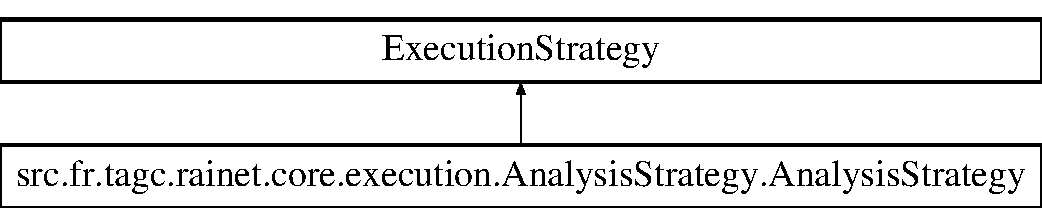
\includegraphics[height=2.000000cm]{classsrc_1_1fr_1_1tagc_1_1rainet_1_1core_1_1execution_1_1AnalysisStrategy_1_1AnalysisStrategy}
\end{center}
\end{figure}
\subsection*{Public Member Functions}
\begin{DoxyCompactItemize}
\item 
\hypertarget{classsrc_1_1fr_1_1tagc_1_1rainet_1_1core_1_1execution_1_1AnalysisStrategy_1_1AnalysisStrategy_ad52de212aa18c8698789ce6550e7bf74}{def {\bfseries \-\_\-\-\_\-init\-\_\-\-\_\-}}\label{classsrc_1_1fr_1_1tagc_1_1rainet_1_1core_1_1execution_1_1AnalysisStrategy_1_1AnalysisStrategy_ad52de212aa18c8698789ce6550e7bf74}

\item 
\hypertarget{classsrc_1_1fr_1_1tagc_1_1rainet_1_1core_1_1execution_1_1AnalysisStrategy_1_1AnalysisStrategy_a4c5d1efe84f1bd827fb964b556f0b096}{def {\bfseries execute}}\label{classsrc_1_1fr_1_1tagc_1_1rainet_1_1core_1_1execution_1_1AnalysisStrategy_1_1AnalysisStrategy_a4c5d1efe84f1bd827fb964b556f0b096}

\item 
\hypertarget{classsrc_1_1fr_1_1tagc_1_1rainet_1_1core_1_1execution_1_1AnalysisStrategy_1_1AnalysisStrategy_afacd1b957334dd17fc1d76d549c5db58}{def {\bfseries analysis}}\label{classsrc_1_1fr_1_1tagc_1_1rainet_1_1core_1_1execution_1_1AnalysisStrategy_1_1AnalysisStrategy_afacd1b957334dd17fc1d76d549c5db58}

\item 
\hypertarget{classsrc_1_1fr_1_1tagc_1_1rainet_1_1core_1_1execution_1_1AnalysisStrategy_1_1AnalysisStrategy_a9caf8769e12327a1977a538b8f524109}{def {\bfseries filter\-\_\-\-R\-N\-A}}\label{classsrc_1_1fr_1_1tagc_1_1rainet_1_1core_1_1execution_1_1AnalysisStrategy_1_1AnalysisStrategy_a9caf8769e12327a1977a538b8f524109}

\item 
\hypertarget{classsrc_1_1fr_1_1tagc_1_1rainet_1_1core_1_1execution_1_1AnalysisStrategy_1_1AnalysisStrategy_a2cb116468db214af7c03d4f5a7c7a561}{def {\bfseries filter\-\_\-protein}}\label{classsrc_1_1fr_1_1tagc_1_1rainet_1_1core_1_1execution_1_1AnalysisStrategy_1_1AnalysisStrategy_a2cb116468db214af7c03d4f5a7c7a561}

\item 
\hypertarget{classsrc_1_1fr_1_1tagc_1_1rainet_1_1core_1_1execution_1_1AnalysisStrategy_1_1AnalysisStrategy_a50e7f51c5879715c53a7c39e3ed7d55b}{def {\bfseries filter\-\_\-\-P\-R\-I}}\label{classsrc_1_1fr_1_1tagc_1_1rainet_1_1core_1_1execution_1_1AnalysisStrategy_1_1AnalysisStrategy_a50e7f51c5879715c53a7c39e3ed7d55b}

\item 
\hypertarget{classsrc_1_1fr_1_1tagc_1_1rainet_1_1core_1_1execution_1_1AnalysisStrategy_1_1AnalysisStrategy_adecc80f4d2f5d4991c0dafa231a87e0a}{def {\bfseries dump\-\_\-filter\-\_\-\-P\-R\-I\-\_\-expression}}\label{classsrc_1_1fr_1_1tagc_1_1rainet_1_1core_1_1execution_1_1AnalysisStrategy_1_1AnalysisStrategy_adecc80f4d2f5d4991c0dafa231a87e0a}

\item 
\hypertarget{classsrc_1_1fr_1_1tagc_1_1rainet_1_1core_1_1execution_1_1AnalysisStrategy_1_1AnalysisStrategy_acfc9442be160e96ebf8a60d93b27a5b7}{def {\bfseries write\-\_\-parameter\-\_\-log}}\label{classsrc_1_1fr_1_1tagc_1_1rainet_1_1core_1_1execution_1_1AnalysisStrategy_1_1AnalysisStrategy_acfc9442be160e96ebf8a60d93b27a5b7}

\item 
\hypertarget{classsrc_1_1fr_1_1tagc_1_1rainet_1_1core_1_1execution_1_1AnalysisStrategy_1_1AnalysisStrategy_ace5475cf3bad8c1a650d6bc620a0246d}{def {\bfseries after\-\_\-filter\-\_\-report}}\label{classsrc_1_1fr_1_1tagc_1_1rainet_1_1core_1_1execution_1_1AnalysisStrategy_1_1AnalysisStrategy_ace5475cf3bad8c1a650d6bc620a0246d}

\item 
\hypertarget{classsrc_1_1fr_1_1tagc_1_1rainet_1_1core_1_1execution_1_1AnalysisStrategy_1_1AnalysisStrategy_a0ce9eb48415167a40b90b52431e1b354}{def {\bfseries interaction\-\_\-report}}\label{classsrc_1_1fr_1_1tagc_1_1rainet_1_1core_1_1execution_1_1AnalysisStrategy_1_1AnalysisStrategy_a0ce9eb48415167a40b90b52431e1b354}

\item 
\hypertarget{classsrc_1_1fr_1_1tagc_1_1rainet_1_1core_1_1execution_1_1AnalysisStrategy_1_1AnalysisStrategy_a969c70813e6fd71c5fdaf957e5f06dfc}{def {\bfseries expression\-\_\-report}}\label{classsrc_1_1fr_1_1tagc_1_1rainet_1_1core_1_1execution_1_1AnalysisStrategy_1_1AnalysisStrategy_a969c70813e6fd71c5fdaf957e5f06dfc}

\item 
\hypertarget{classsrc_1_1fr_1_1tagc_1_1rainet_1_1core_1_1execution_1_1AnalysisStrategy_1_1AnalysisStrategy_aabb116b5befca1f6ed5639073400db69}{def {\bfseries write\-\_\-report}}\label{classsrc_1_1fr_1_1tagc_1_1rainet_1_1core_1_1execution_1_1AnalysisStrategy_1_1AnalysisStrategy_aabb116b5befca1f6ed5639073400db69}

\end{DoxyCompactItemize}
\subsection*{Public Attributes}
\begin{DoxyCompactItemize}
\item 
\hypertarget{classsrc_1_1fr_1_1tagc_1_1rainet_1_1core_1_1execution_1_1AnalysisStrategy_1_1AnalysisStrategy_a8ee9e3e09359b167db4475b7180f9da9}{{\bfseries write\-Report\-File}}\label{classsrc_1_1fr_1_1tagc_1_1rainet_1_1core_1_1execution_1_1AnalysisStrategy_1_1AnalysisStrategy_a8ee9e3e09359b167db4475b7180f9da9}

\item 
\hypertarget{classsrc_1_1fr_1_1tagc_1_1rainet_1_1core_1_1execution_1_1AnalysisStrategy_1_1AnalysisStrategy_a8a12304c4731dde95c55fdc2ceb858f5}{{\bfseries D\-B\-Path}}\label{classsrc_1_1fr_1_1tagc_1_1rainet_1_1core_1_1execution_1_1AnalysisStrategy_1_1AnalysisStrategy_a8a12304c4731dde95c55fdc2ceb858f5}

\item 
\hypertarget{classsrc_1_1fr_1_1tagc_1_1rainet_1_1core_1_1execution_1_1AnalysisStrategy_1_1AnalysisStrategy_a593720d68550ba843e97f2520c30aa19}{{\bfseries species}}\label{classsrc_1_1fr_1_1tagc_1_1rainet_1_1core_1_1execution_1_1AnalysisStrategy_1_1AnalysisStrategy_a593720d68550ba843e97f2520c30aa19}

\item 
\hypertarget{classsrc_1_1fr_1_1tagc_1_1rainet_1_1core_1_1execution_1_1AnalysisStrategy_1_1AnalysisStrategy_a1a458f3522615ca796eb28e2cdbccfa9}{{\bfseries output\-Folder}}\label{classsrc_1_1fr_1_1tagc_1_1rainet_1_1core_1_1execution_1_1AnalysisStrategy_1_1AnalysisStrategy_a1a458f3522615ca796eb28e2cdbccfa9}

\item 
\hypertarget{classsrc_1_1fr_1_1tagc_1_1rainet_1_1core_1_1execution_1_1AnalysisStrategy_1_1AnalysisStrategy_acc531a802815eed37200c15db9c22f9e}{{\bfseries minimum\-Interaction\-Score}}\label{classsrc_1_1fr_1_1tagc_1_1rainet_1_1core_1_1execution_1_1AnalysisStrategy_1_1AnalysisStrategy_acc531a802815eed37200c15db9c22f9e}

\item 
\hypertarget{classsrc_1_1fr_1_1tagc_1_1rainet_1_1core_1_1execution_1_1AnalysisStrategy_1_1AnalysisStrategy_aaf30beb4d95bd29d2cfe3d4bc555fd5a}{{\bfseries R\-N\-A\-Biotypes}}\label{classsrc_1_1fr_1_1tagc_1_1rainet_1_1core_1_1execution_1_1AnalysisStrategy_1_1AnalysisStrategy_aaf30beb4d95bd29d2cfe3d4bc555fd5a}

\item 
\hypertarget{classsrc_1_1fr_1_1tagc_1_1rainet_1_1core_1_1execution_1_1AnalysisStrategy_1_1AnalysisStrategy_a4bdb5ae6218d58958621b33925c8b142}{{\bfseries gencode}}\label{classsrc_1_1fr_1_1tagc_1_1rainet_1_1core_1_1execution_1_1AnalysisStrategy_1_1AnalysisStrategy_a4bdb5ae6218d58958621b33925c8b142}

\item 
\hypertarget{classsrc_1_1fr_1_1tagc_1_1rainet_1_1core_1_1execution_1_1AnalysisStrategy_1_1AnalysisStrategy_aae02c6160d659af00120b45b508f1c14}{{\bfseries expression\-Value\-Cutoff}}\label{classsrc_1_1fr_1_1tagc_1_1rainet_1_1core_1_1execution_1_1AnalysisStrategy_1_1AnalysisStrategy_aae02c6160d659af00120b45b508f1c14}

\item 
\hypertarget{classsrc_1_1fr_1_1tagc_1_1rainet_1_1core_1_1execution_1_1AnalysisStrategy_1_1AnalysisStrategy_aa932e7b6f4e0d75dce4c35467d5429b6}{{\bfseries expression\-Tissue\-Cutoff}}\label{classsrc_1_1fr_1_1tagc_1_1rainet_1_1core_1_1execution_1_1AnalysisStrategy_1_1AnalysisStrategy_aa932e7b6f4e0d75dce4c35467d5429b6}

\item 
\hypertarget{classsrc_1_1fr_1_1tagc_1_1rainet_1_1core_1_1execution_1_1AnalysisStrategy_1_1AnalysisStrategy_a2debf5e9794995a58f4204c106fdd3ee}{\hyperlink{classsrc_1_1fr_1_1tagc_1_1rainet_1_1core_1_1execution_1_1AnalysisStrategy_1_1AnalysisStrategy_a2debf5e9794995a58f4204c106fdd3ee}{low\-Memory}}\label{classsrc_1_1fr_1_1tagc_1_1rainet_1_1core_1_1execution_1_1AnalysisStrategy_1_1AnalysisStrategy_a2debf5e9794995a58f4204c106fdd3ee}

\begin{DoxyCompactList}\small\item\em write last batch if using low memory flag \end{DoxyCompactList}\item 
\hypertarget{classsrc_1_1fr_1_1tagc_1_1rainet_1_1core_1_1execution_1_1AnalysisStrategy_1_1AnalysisStrategy_a3380fdee307e1339386720e45a51f5d1}{{\bfseries arguments}}\label{classsrc_1_1fr_1_1tagc_1_1rainet_1_1core_1_1execution_1_1AnalysisStrategy_1_1AnalysisStrategy_a3380fdee307e1339386720e45a51f5d1}

\item 
\hypertarget{classsrc_1_1fr_1_1tagc_1_1rainet_1_1core_1_1execution_1_1AnalysisStrategy_1_1AnalysisStrategy_a794dd2d4016eed8757da5367b485123d}{{\bfseries output\-Folder\-Report}}\label{classsrc_1_1fr_1_1tagc_1_1rainet_1_1core_1_1execution_1_1AnalysisStrategy_1_1AnalysisStrategy_a794dd2d4016eed8757da5367b485123d}

\item 
\hypertarget{classsrc_1_1fr_1_1tagc_1_1rainet_1_1core_1_1execution_1_1AnalysisStrategy_1_1AnalysisStrategy_abf707cc43891f681e507b5f83ff844c4}{{\bfseries sql\-\_\-session}}\label{classsrc_1_1fr_1_1tagc_1_1rainet_1_1core_1_1execution_1_1AnalysisStrategy_1_1AnalysisStrategy_abf707cc43891f681e507b5f83ff844c4}

\item 
\hypertarget{classsrc_1_1fr_1_1tagc_1_1rainet_1_1core_1_1execution_1_1AnalysisStrategy_1_1AnalysisStrategy_ae91540e0a0023c9294991039ec40230a}{{\bfseries db\-\_\-engine}}\label{classsrc_1_1fr_1_1tagc_1_1rainet_1_1core_1_1execution_1_1AnalysisStrategy_1_1AnalysisStrategy_ae91540e0a0023c9294991039ec40230a}

\item 
\hypertarget{classsrc_1_1fr_1_1tagc_1_1rainet_1_1core_1_1execution_1_1AnalysisStrategy_1_1AnalysisStrategy_a20aa5e4df0dba3402e6d68de24376556}{{\bfseries m\-R\-N\-A\-Dict}}\label{classsrc_1_1fr_1_1tagc_1_1rainet_1_1core_1_1execution_1_1AnalysisStrategy_1_1AnalysisStrategy_a20aa5e4df0dba3402e6d68de24376556}

\item 
\hypertarget{classsrc_1_1fr_1_1tagc_1_1rainet_1_1core_1_1execution_1_1AnalysisStrategy_1_1AnalysisStrategy_a1ac11446e39a71a08d726e80bc9c8712}{{\bfseries expression\-Dict}}\label{classsrc_1_1fr_1_1tagc_1_1rainet_1_1core_1_1execution_1_1AnalysisStrategy_1_1AnalysisStrategy_a1ac11446e39a71a08d726e80bc9c8712}

\item 
\hypertarget{classsrc_1_1fr_1_1tagc_1_1rainet_1_1core_1_1execution_1_1AnalysisStrategy_1_1AnalysisStrategy_adde38952ec8433c31a58864155dcb961}{{\bfseries Prot\-M\-R\-N\-A\-Tissue\-Expressions}}\label{classsrc_1_1fr_1_1tagc_1_1rainet_1_1core_1_1execution_1_1AnalysisStrategy_1_1AnalysisStrategy_adde38952ec8433c31a58864155dcb961}

\end{DoxyCompactItemize}
\subsection*{Static Public Attributes}
\begin{DoxyCompactItemize}
\item 
\hypertarget{classsrc_1_1fr_1_1tagc_1_1rainet_1_1core_1_1execution_1_1AnalysisStrategy_1_1AnalysisStrategy_ae17c250cc20d36bf89f9580e38a28e73}{string {\bfseries R\-N\-A\-\_\-\-A\-L\-L\-\_\-\-K\-W} = \char`\"{}all\-R\-N\-As\char`\"{}}\label{classsrc_1_1fr_1_1tagc_1_1rainet_1_1core_1_1execution_1_1AnalysisStrategy_1_1AnalysisStrategy_ae17c250cc20d36bf89f9580e38a28e73}

\item 
\hypertarget{classsrc_1_1fr_1_1tagc_1_1rainet_1_1core_1_1execution_1_1AnalysisStrategy_1_1AnalysisStrategy_a79d55019a836f55d7334f4aa903dc664}{string {\bfseries P\-R\-O\-T\-\_\-\-A\-L\-L\-\_\-\-K\-W} = \char`\"{}all\-Proteins\char`\"{}}\label{classsrc_1_1fr_1_1tagc_1_1rainet_1_1core_1_1execution_1_1AnalysisStrategy_1_1AnalysisStrategy_a79d55019a836f55d7334f4aa903dc664}

\item 
\hypertarget{classsrc_1_1fr_1_1tagc_1_1rainet_1_1core_1_1execution_1_1AnalysisStrategy_1_1AnalysisStrategy_ad4a1038f35ca4aa43d2d23c2dc276fc0}{string {\bfseries R\-N\-A\-\_\-\-F\-I\-L\-T\-E\-R\-\_\-\-K\-W} = \char`\"{}selected\-R\-N\-As\char`\"{}}\label{classsrc_1_1fr_1_1tagc_1_1rainet_1_1core_1_1execution_1_1AnalysisStrategy_1_1AnalysisStrategy_ad4a1038f35ca4aa43d2d23c2dc276fc0}

\item 
\hypertarget{classsrc_1_1fr_1_1tagc_1_1rainet_1_1core_1_1execution_1_1AnalysisStrategy_1_1AnalysisStrategy_ac131822dabafbde99fd79c4937a68353}{string {\bfseries R\-N\-A\-\_\-\-F\-I\-L\-T\-E\-R\-\_\-\-K\-E\-Y\-\_\-\-K\-W} = \char`\"{}selected\-R\-N\-As\-Key\char`\"{}}\label{classsrc_1_1fr_1_1tagc_1_1rainet_1_1core_1_1execution_1_1AnalysisStrategy_1_1AnalysisStrategy_ac131822dabafbde99fd79c4937a68353}

\item 
\hypertarget{classsrc_1_1fr_1_1tagc_1_1rainet_1_1core_1_1execution_1_1AnalysisStrategy_1_1AnalysisStrategy_ac099830f4f6add2eefe20a2f985a2663}{string {\bfseries P\-R\-O\-T\-\_\-\-F\-I\-L\-T\-E\-R\-\_\-\-K\-W} = \char`\"{}selected\-Proteins\char`\"{}}\label{classsrc_1_1fr_1_1tagc_1_1rainet_1_1core_1_1execution_1_1AnalysisStrategy_1_1AnalysisStrategy_ac099830f4f6add2eefe20a2f985a2663}

\item 
\hypertarget{classsrc_1_1fr_1_1tagc_1_1rainet_1_1core_1_1execution_1_1AnalysisStrategy_1_1AnalysisStrategy_a558ca5d2d066eea48f1edb0d50387c9a}{string {\bfseries P\-R\-O\-T\-\_\-\-F\-I\-L\-T\-E\-R\-\_\-\-K\-E\-Y\-\_\-\-K\-W} = \char`\"{}selected\-Proteins\-Key\char`\"{}}\label{classsrc_1_1fr_1_1tagc_1_1rainet_1_1core_1_1execution_1_1AnalysisStrategy_1_1AnalysisStrategy_a558ca5d2d066eea48f1edb0d50387c9a}

\item 
\hypertarget{classsrc_1_1fr_1_1tagc_1_1rainet_1_1core_1_1execution_1_1AnalysisStrategy_1_1AnalysisStrategy_a03520ac898660e05a2b7e45c97d34ade}{string {\bfseries P\-R\-I\-\_\-\-P\-R\-O\-T\-\_\-\-A\-L\-L\-\_\-\-K\-W} = \char`\"{}all\-Proteins\-In\-Interaction\-Table\char`\"{}}\label{classsrc_1_1fr_1_1tagc_1_1rainet_1_1core_1_1execution_1_1AnalysisStrategy_1_1AnalysisStrategy_a03520ac898660e05a2b7e45c97d34ade}

\item 
\hypertarget{classsrc_1_1fr_1_1tagc_1_1rainet_1_1core_1_1execution_1_1AnalysisStrategy_1_1AnalysisStrategy_a875965a6bda91d8eb6c121078b1f9fbd}{string {\bfseries P\-R\-I\-\_\-\-R\-N\-A\-\_\-\-A\-L\-L\-\_\-\-K\-W} = \char`\"{}all\-R\-N\-A\-In\-Interaction\-Table\char`\"{}}\label{classsrc_1_1fr_1_1tagc_1_1rainet_1_1core_1_1execution_1_1AnalysisStrategy_1_1AnalysisStrategy_a875965a6bda91d8eb6c121078b1f9fbd}

\item 
\hypertarget{classsrc_1_1fr_1_1tagc_1_1rainet_1_1core_1_1execution_1_1AnalysisStrategy_1_1AnalysisStrategy_ad973bcc1dbbdbb9930e14dde4786dab7}{string {\bfseries P\-R\-I\-\_\-\-F\-I\-L\-T\-E\-R\-\_\-\-K\-W} = \char`\"{}selected\-Interactions\char`\"{}}\label{classsrc_1_1fr_1_1tagc_1_1rainet_1_1core_1_1execution_1_1AnalysisStrategy_1_1AnalysisStrategy_ad973bcc1dbbdbb9930e14dde4786dab7}

\item 
\hypertarget{classsrc_1_1fr_1_1tagc_1_1rainet_1_1core_1_1execution_1_1AnalysisStrategy_1_1AnalysisStrategy_a6605b1ff38398aad67c54581ec3d1fe2}{string {\bfseries P\-R\-I\-\_\-\-P\-R\-O\-T\-\_\-\-F\-I\-L\-T\-E\-R\-\_\-\-K\-W} = \char`\"{}filtered\-Interacting\-Proteins\char`\"{}}\label{classsrc_1_1fr_1_1tagc_1_1rainet_1_1core_1_1execution_1_1AnalysisStrategy_1_1AnalysisStrategy_a6605b1ff38398aad67c54581ec3d1fe2}

\item 
\hypertarget{classsrc_1_1fr_1_1tagc_1_1rainet_1_1core_1_1execution_1_1AnalysisStrategy_1_1AnalysisStrategy_a7010ee293392369ad5153bf401c41f4e}{string {\bfseries P\-R\-I\-\_\-\-R\-N\-A\-\_\-\-F\-I\-L\-T\-E\-R\-\_\-\-K\-W} = \char`\"{}filtered\-Interacting\-R\-N\-As\char`\"{}}\label{classsrc_1_1fr_1_1tagc_1_1rainet_1_1core_1_1execution_1_1AnalysisStrategy_1_1AnalysisStrategy_a7010ee293392369ad5153bf401c41f4e}

\item 
\hypertarget{classsrc_1_1fr_1_1tagc_1_1rainet_1_1core_1_1execution_1_1AnalysisStrategy_1_1AnalysisStrategy_a6977a65ee6905c26f387cd1f3a137cec}{string {\bfseries P\-R\-O\-T\-\_\-\-T\-I\-S\-S\-U\-E\-S\-\_\-\-K\-W} = \char`\"{}protein\-Tissues\char`\"{}}\label{classsrc_1_1fr_1_1tagc_1_1rainet_1_1core_1_1execution_1_1AnalysisStrategy_1_1AnalysisStrategy_a6977a65ee6905c26f387cd1f3a137cec}

\item 
\hypertarget{classsrc_1_1fr_1_1tagc_1_1rainet_1_1core_1_1execution_1_1AnalysisStrategy_1_1AnalysisStrategy_aaff43d3017d781f56e05654c0afde756}{string {\bfseries R\-N\-A\-\_\-\-T\-I\-S\-S\-U\-E\-S\-\_\-\-K\-W} = \char`\"{}rna\-Tissues\char`\"{}}\label{classsrc_1_1fr_1_1tagc_1_1rainet_1_1core_1_1execution_1_1AnalysisStrategy_1_1AnalysisStrategy_aaff43d3017d781f56e05654c0afde756}

\item 
\hypertarget{classsrc_1_1fr_1_1tagc_1_1rainet_1_1core_1_1execution_1_1AnalysisStrategy_1_1AnalysisStrategy_a3589add90344e40d39f5f1476b50fceb}{string {\bfseries P\-R\-I\-\_\-\-T\-I\-S\-S\-U\-E\-S\-\_\-\-K\-W} = \char`\"{}interacting\-Tissues\char`\"{}}\label{classsrc_1_1fr_1_1tagc_1_1rainet_1_1core_1_1execution_1_1AnalysisStrategy_1_1AnalysisStrategy_a3589add90344e40d39f5f1476b50fceb}

\item 
\hypertarget{classsrc_1_1fr_1_1tagc_1_1rainet_1_1core_1_1execution_1_1AnalysisStrategy_1_1AnalysisStrategy_acda18a97f22998f1c6cfba1223e9b7b2}{string {\bfseries F\-I\-N\-A\-L\-\_\-\-P\-R\-O\-\_\-\-K\-W} = \char`\"{}final\-Proteins\char`\"{}}\label{classsrc_1_1fr_1_1tagc_1_1rainet_1_1core_1_1execution_1_1AnalysisStrategy_1_1AnalysisStrategy_acda18a97f22998f1c6cfba1223e9b7b2}

\item 
\hypertarget{classsrc_1_1fr_1_1tagc_1_1rainet_1_1core_1_1execution_1_1AnalysisStrategy_1_1AnalysisStrategy_afea3892d2c2b923637411886290cfd9d}{string {\bfseries F\-I\-N\-A\-L\-\_\-\-R\-N\-A\-\_\-\-K\-W} = \char`\"{}final\-R\-N\-As\char`\"{}}\label{classsrc_1_1fr_1_1tagc_1_1rainet_1_1core_1_1execution_1_1AnalysisStrategy_1_1AnalysisStrategy_afea3892d2c2b923637411886290cfd9d}

\item 
\hypertarget{classsrc_1_1fr_1_1tagc_1_1rainet_1_1core_1_1execution_1_1AnalysisStrategy_1_1AnalysisStrategy_af6f22b3a9df7daa85b2487a390021857}{string {\bfseries R\-\_\-\-W\-O\-R\-K\-I\-N\-G\-\_\-\-D\-I\-R} = \char`\"{}/home/diogo/workspace/tagc-\/rainet-\/R\-N\-A/src/fr/tagc/rainet/core/execution/analysis/Rscripts/\char`\"{}}\label{classsrc_1_1fr_1_1tagc_1_1rainet_1_1core_1_1execution_1_1AnalysisStrategy_1_1AnalysisStrategy_af6f22b3a9df7daa85b2487a390021857}

\item 
\hypertarget{classsrc_1_1fr_1_1tagc_1_1rainet_1_1core_1_1execution_1_1AnalysisStrategy_1_1AnalysisStrategy_aee9e4e19e7aaa820a99b553292ec53a9}{string {\bfseries R\-\_\-\-M\-A\-I\-N\-\_\-\-S\-C\-R\-I\-P\-T} = \char`\"{}/home/diogo/workspace/tagc-\/rainet-\/R\-N\-A/src/fr/tagc/rainet/core/execution/analysis/Rscripts/analysis\-\_\-strategy\-\_\-report.\-R\char`\"{}}\label{classsrc_1_1fr_1_1tagc_1_1rainet_1_1core_1_1execution_1_1AnalysisStrategy_1_1AnalysisStrategy_aee9e4e19e7aaa820a99b553292ec53a9}

\item 
\hypertarget{classsrc_1_1fr_1_1tagc_1_1rainet_1_1core_1_1execution_1_1AnalysisStrategy_1_1AnalysisStrategy_a02454a0f78fd3fa370ddc31369f3468e}{string {\bfseries R\-\_\-\-S\-W\-E\-A\-V\-E\-\_\-\-F\-I\-L\-E} = \char`\"{}/home/diogo/workspace/tagc-\/rainet-\/R\-N\-A/src/fr/tagc/rainet/core/execution/analysis/Rscripts/analysis\-\_\-strategy\-\_\-report.\-Rnw\char`\"{}}\label{classsrc_1_1fr_1_1tagc_1_1rainet_1_1core_1_1execution_1_1AnalysisStrategy_1_1AnalysisStrategy_a02454a0f78fd3fa370ddc31369f3468e}

\item 
\hypertarget{classsrc_1_1fr_1_1tagc_1_1rainet_1_1core_1_1execution_1_1AnalysisStrategy_1_1AnalysisStrategy_a2cdd064a0f2e10ddc315085bdff7af78}{string {\bfseries P\-A\-R\-A\-M\-E\-T\-E\-R\-S\-\_\-\-L\-O\-G} = \char`\"{}parameters.\-log\char`\"{}}\label{classsrc_1_1fr_1_1tagc_1_1rainet_1_1core_1_1execution_1_1AnalysisStrategy_1_1AnalysisStrategy_a2cdd064a0f2e10ddc315085bdff7af78}

\item 
\hypertarget{classsrc_1_1fr_1_1tagc_1_1rainet_1_1core_1_1execution_1_1AnalysisStrategy_1_1AnalysisStrategy_abd70bcf568587fbe767deb268ad3049b}{string {\bfseries R\-E\-P\-O\-R\-T\-\_\-\-R\-N\-A\-\_\-\-N\-U\-M\-B\-E\-R\-S} = \char`\"{}rna\-\_\-numbers.\-tsv\char`\"{}}\label{classsrc_1_1fr_1_1tagc_1_1rainet_1_1core_1_1execution_1_1AnalysisStrategy_1_1AnalysisStrategy_abd70bcf568587fbe767deb268ad3049b}

\item 
\hypertarget{classsrc_1_1fr_1_1tagc_1_1rainet_1_1core_1_1execution_1_1AnalysisStrategy_1_1AnalysisStrategy_a59dc2f8719c4b499f987b138b0e512cf}{string {\bfseries R\-E\-P\-O\-R\-T\-\_\-\-R\-N\-A\-\_\-\-L\-I\-S\-T\-\_\-\-A\-F\-T\-E\-R\-\_\-\-R\-N\-A\-\_\-\-F\-I\-L\-T\-E\-R} = \char`\"{}list\-\_\-\-R\-N\-As\-\_\-after\-\_\-\-R\-N\-A\-\_\-filter.\-tsv\char`\"{}}\label{classsrc_1_1fr_1_1tagc_1_1rainet_1_1core_1_1execution_1_1AnalysisStrategy_1_1AnalysisStrategy_a59dc2f8719c4b499f987b138b0e512cf}

\item 
\hypertarget{classsrc_1_1fr_1_1tagc_1_1rainet_1_1core_1_1execution_1_1AnalysisStrategy_1_1AnalysisStrategy_aee7f68ef784ed9d1e4765234d599fe59}{string {\bfseries R\-E\-P\-O\-R\-T\-\_\-\-P\-R\-O\-T\-E\-I\-N\-\_\-\-L\-I\-S\-T\-\_\-\-A\-F\-T\-E\-R\-\_\-\-P\-R\-O\-T\-E\-I\-N\-\_\-\-F\-I\-L\-T\-E\-R} = \char`\"{}list\-\_\-proteins\-\_\-after\-\_\-protein\-\_\-filter.\-tsv\char`\"{}}\label{classsrc_1_1fr_1_1tagc_1_1rainet_1_1core_1_1execution_1_1AnalysisStrategy_1_1AnalysisStrategy_aee7f68ef784ed9d1e4765234d599fe59}

\item 
\hypertarget{classsrc_1_1fr_1_1tagc_1_1rainet_1_1core_1_1execution_1_1AnalysisStrategy_1_1AnalysisStrategy_a8753a6c83671c7edf56b5945529dede4}{string {\bfseries R\-E\-P\-O\-R\-T\-\_\-\-I\-N\-T\-E\-R\-A\-C\-T\-I\-O\-N\-\_\-\-N\-U\-M\-B\-E\-R\-S} = \char`\"{}interaction\-\_\-numbers.\-tsv\char`\"{}}\label{classsrc_1_1fr_1_1tagc_1_1rainet_1_1core_1_1execution_1_1AnalysisStrategy_1_1AnalysisStrategy_a8753a6c83671c7edf56b5945529dede4}

\item 
\hypertarget{classsrc_1_1fr_1_1tagc_1_1rainet_1_1core_1_1execution_1_1AnalysisStrategy_1_1AnalysisStrategy_aa9c97f0191f79331495adbe95b5a3bbf}{string {\bfseries R\-E\-P\-O\-R\-T\-\_\-\-R\-N\-A\-\_\-\-E\-X\-P\-R\-E\-S\-S\-I\-O\-N} = \char`\"{}rna\-\_\-expression.\-tsv\char`\"{}}\label{classsrc_1_1fr_1_1tagc_1_1rainet_1_1core_1_1execution_1_1AnalysisStrategy_1_1AnalysisStrategy_aa9c97f0191f79331495adbe95b5a3bbf}

\item 
\hypertarget{classsrc_1_1fr_1_1tagc_1_1rainet_1_1core_1_1execution_1_1AnalysisStrategy_1_1AnalysisStrategy_ae5e69144a18e711d130e9a985b166eb5}{string {\bfseries R\-E\-P\-O\-R\-T\-\_\-\-R\-N\-A\-\_\-\-E\-X\-P\-R\-E\-S\-S\-I\-O\-N\-\_\-\-D\-A\-T\-A\-\_\-\-P\-R\-E\-S\-E\-N\-C\-E} = \char`\"{}rna\-\_\-expression\-\_\-data\-\_\-presence.\-tsv\char`\"{}}\label{classsrc_1_1fr_1_1tagc_1_1rainet_1_1core_1_1execution_1_1AnalysisStrategy_1_1AnalysisStrategy_ae5e69144a18e711d130e9a985b166eb5}

\item 
\hypertarget{classsrc_1_1fr_1_1tagc_1_1rainet_1_1core_1_1execution_1_1AnalysisStrategy_1_1AnalysisStrategy_af7aefdde072f83459c98f8df759f1d4e}{string {\bfseries R\-E\-P\-O\-R\-T\-\_\-\-T\-I\-S\-S\-U\-E\-S\-\_\-\-W\-H\-E\-R\-E\-\_\-\-E\-X\-P\-R\-E\-S\-S\-E\-D} = \char`\"{}interactions\-\_\-tissues\-\_\-where\-\_\-expressed.\-tsv\char`\"{}}\label{classsrc_1_1fr_1_1tagc_1_1rainet_1_1core_1_1execution_1_1AnalysisStrategy_1_1AnalysisStrategy_af7aefdde072f83459c98f8df759f1d4e}

\item 
\hypertarget{classsrc_1_1fr_1_1tagc_1_1rainet_1_1core_1_1execution_1_1AnalysisStrategy_1_1AnalysisStrategy_a13c7700025c615387b9b51122fc39c67}{string {\bfseries R\-E\-P\-O\-R\-T\-\_\-\-P\-R\-O\-T\-E\-I\-N\-S\-\_\-\-E\-X\-P\-R\-E\-S\-S\-E\-D\-\_\-\-P\-E\-R\-\_\-\-T\-I\-S\-S\-U\-E} = \char`\"{}proteins\-\_\-expressed\-\_\-per\-\_\-tissue.\-tsv\char`\"{}}\label{classsrc_1_1fr_1_1tagc_1_1rainet_1_1core_1_1execution_1_1AnalysisStrategy_1_1AnalysisStrategy_a13c7700025c615387b9b51122fc39c67}

\item 
\hypertarget{classsrc_1_1fr_1_1tagc_1_1rainet_1_1core_1_1execution_1_1AnalysisStrategy_1_1AnalysisStrategy_a2e8330a93ba684a2915ee4d402b579a3}{string {\bfseries R\-E\-P\-O\-R\-T\-\_\-\-R\-N\-A\-S\-\_\-\-E\-X\-P\-R\-E\-S\-S\-E\-D\-\_\-\-P\-E\-R\-\_\-\-T\-I\-S\-S\-U\-E} = \char`\"{}rnas\-\_\-expressed\-\_\-per\-\_\-tissue.\-tsv\char`\"{}}\label{classsrc_1_1fr_1_1tagc_1_1rainet_1_1core_1_1execution_1_1AnalysisStrategy_1_1AnalysisStrategy_a2e8330a93ba684a2915ee4d402b579a3}

\item 
\hypertarget{classsrc_1_1fr_1_1tagc_1_1rainet_1_1core_1_1execution_1_1AnalysisStrategy_1_1AnalysisStrategy_a3d3103dff33b0add702eff9256a936a6}{string {\bfseries R\-E\-P\-O\-R\-T\-\_\-\-I\-N\-T\-E\-R\-A\-C\-T\-I\-O\-N\-\_\-\-S\-C\-O\-R\-E\-S\-\_\-\-B\-I\-O\-T\-Y\-P\-E} = \char`\"{}interaction\-\_\-scores\-\_\-biotype.\-tsv\char`\"{}}\label{classsrc_1_1fr_1_1tagc_1_1rainet_1_1core_1_1execution_1_1AnalysisStrategy_1_1AnalysisStrategy_a3d3103dff33b0add702eff9256a936a6}

\item 
\hypertarget{classsrc_1_1fr_1_1tagc_1_1rainet_1_1core_1_1execution_1_1AnalysisStrategy_1_1AnalysisStrategy_ab364e8bc96e50882f673acf510ad6d9d}{string {\bfseries R\-E\-P\-O\-R\-T\-\_\-\-I\-N\-T\-E\-R\-A\-C\-T\-I\-O\-N\-\_\-\-P\-A\-R\-T\-N\-E\-R\-S\-\_\-\-B\-I\-O\-T\-Y\-P\-E} = \char`\"{}interaction\-\_\-partners\-\_\-biotype.\-tsv\char`\"{}}\label{classsrc_1_1fr_1_1tagc_1_1rainet_1_1core_1_1execution_1_1AnalysisStrategy_1_1AnalysisStrategy_ab364e8bc96e50882f673acf510ad6d9d}

\item 
\hypertarget{classsrc_1_1fr_1_1tagc_1_1rainet_1_1core_1_1execution_1_1AnalysisStrategy_1_1AnalysisStrategy_aac6522a8d987e324837ee96dfc50d34b}{string {\bfseries R\-E\-P\-O\-R\-T\-\_\-\-I\-N\-T\-E\-R\-A\-C\-T\-I\-O\-N\-S\-\_\-\-S\-C\-O\-R\-E\-\_\-\-M\-A\-T\-R\-I\-X} = \char`\"{}interaction\-\_\-score\-\_\-matrix.\-tsv\char`\"{}}\label{classsrc_1_1fr_1_1tagc_1_1rainet_1_1core_1_1execution_1_1AnalysisStrategy_1_1AnalysisStrategy_aac6522a8d987e324837ee96dfc50d34b}

\item 
\hypertarget{classsrc_1_1fr_1_1tagc_1_1rainet_1_1core_1_1execution_1_1AnalysisStrategy_1_1AnalysisStrategy_a94d05e5c8b5236231c62e7248f69db06}{string {\bfseries D\-U\-M\-P\-\_\-\-E\-X\-P\-R\-E\-S\-S\-I\-O\-N\-\_\-\-F\-I\-L\-T\-E\-R} = \char`\"{}interactions\-\_\-expression\-\_\-filter.\-tsv\char`\"{}}\label{classsrc_1_1fr_1_1tagc_1_1rainet_1_1core_1_1execution_1_1AnalysisStrategy_1_1AnalysisStrategy_a94d05e5c8b5236231c62e7248f69db06}

\item 
\hypertarget{classsrc_1_1fr_1_1tagc_1_1rainet_1_1core_1_1execution_1_1AnalysisStrategy_1_1AnalysisStrategy_a3b3f118c83af80dda56406bb1802b85e}{string {\bfseries D\-U\-M\-P\-\_\-\-E\-X\-P\-R\-E\-S\-S\-I\-O\-N} = \char`\"{}interactions\-\_\-expression.\-tsv\char`\"{}}\label{classsrc_1_1fr_1_1tagc_1_1rainet_1_1core_1_1execution_1_1AnalysisStrategy_1_1AnalysisStrategy_a3b3f118c83af80dda56406bb1802b85e}

\item 
\hypertarget{classsrc_1_1fr_1_1tagc_1_1rainet_1_1core_1_1execution_1_1AnalysisStrategy_1_1AnalysisStrategy_a383d323d89a2701c523d4a5aeebdc1eb}{int {\bfseries D\-U\-M\-P\-\_\-\-E\-X\-P\-R\-E\-S\-S\-I\-O\-N\-\_\-\-F\-I\-L\-T\-E\-R\-\_\-\-B\-A\-T\-C\-H\-\_\-\-S\-I\-Z\-E} = 100}\label{classsrc_1_1fr_1_1tagc_1_1rainet_1_1core_1_1execution_1_1AnalysisStrategy_1_1AnalysisStrategy_a383d323d89a2701c523d4a5aeebdc1eb}

\end{DoxyCompactItemize}


The documentation for this class was generated from the following file\-:\begin{DoxyCompactItemize}
\item 
src/fr/tagc/rainet/core/execution/Analysis\-Strategy.\-py\end{DoxyCompactItemize}

\hypertarget{classAnalysisStrategyUnittest_1_1AnalysisStrategyUnittest}{\section{Analysis\-Strategy\-Unittest.\-Analysis\-Strategy\-Unittest Class Reference}
\label{classAnalysisStrategyUnittest_1_1AnalysisStrategyUnittest}\index{Analysis\-Strategy\-Unittest.\-Analysis\-Strategy\-Unittest@{Analysis\-Strategy\-Unittest.\-Analysis\-Strategy\-Unittest}}
}
Inheritance diagram for Analysis\-Strategy\-Unittest.\-Analysis\-Strategy\-Unittest\-:\begin{figure}[H]
\begin{center}
\leavevmode
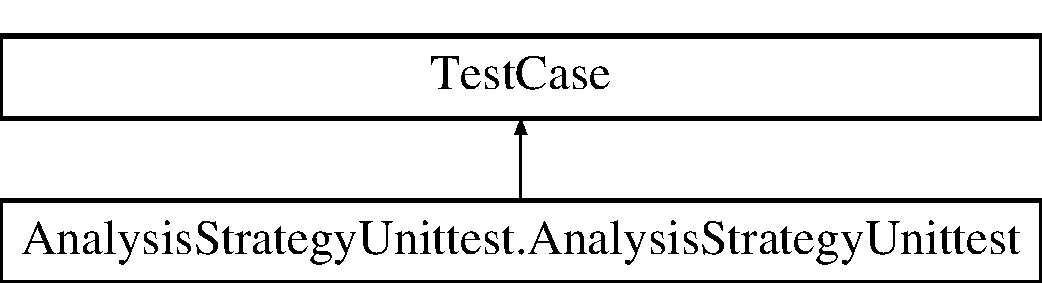
\includegraphics[height=2.000000cm]{classAnalysisStrategyUnittest_1_1AnalysisStrategyUnittest}
\end{center}
\end{figure}
\subsection*{Public Member Functions}
\begin{DoxyCompactItemize}
\item 
\hypertarget{classAnalysisStrategyUnittest_1_1AnalysisStrategyUnittest_a2006669c348f31e397b3efc09f2a0c8b}{def {\bfseries set\-Up}}\label{classAnalysisStrategyUnittest_1_1AnalysisStrategyUnittest_a2006669c348f31e397b3efc09f2a0c8b}

\item 
\hypertarget{classAnalysisStrategyUnittest_1_1AnalysisStrategyUnittest_a4a63e2669aa984b38518587d4127b007}{def {\bfseries test\-\_\-default\-\_\-params}}\label{classAnalysisStrategyUnittest_1_1AnalysisStrategyUnittest_a4a63e2669aa984b38518587d4127b007}

\item 
\hypertarget{classAnalysisStrategyUnittest_1_1AnalysisStrategyUnittest_a3f667212f8ba502ac56ba059d86c3c3d}{def {\bfseries test\-\_\-\-R\-N\-A\-\_\-filter\-\_\-one}}\label{classAnalysisStrategyUnittest_1_1AnalysisStrategyUnittest_a3f667212f8ba502ac56ba059d86c3c3d}

\item 
\hypertarget{classAnalysisStrategyUnittest_1_1AnalysisStrategyUnittest_aecdf1bb6491dba75510e82a6aa903bc5}{def {\bfseries test\-\_\-\-R\-N\-A\-\_\-filter\-\_\-two}}\label{classAnalysisStrategyUnittest_1_1AnalysisStrategyUnittest_aecdf1bb6491dba75510e82a6aa903bc5}

\item 
\hypertarget{classAnalysisStrategyUnittest_1_1AnalysisStrategyUnittest_a6826d8d8c3388a01d0a89d8012b3cee0}{def {\bfseries test\-\_\-\-R\-N\-A\-\_\-filter\-\_\-four}}\label{classAnalysisStrategyUnittest_1_1AnalysisStrategyUnittest_a6826d8d8c3388a01d0a89d8012b3cee0}

\item 
\hypertarget{classAnalysisStrategyUnittest_1_1AnalysisStrategyUnittest_aa01ac03294b445706622e6e8902f041e}{def {\bfseries test\-\_\-\-P\-R\-I\-\_\-filter\-\_\-one}}\label{classAnalysisStrategyUnittest_1_1AnalysisStrategyUnittest_aa01ac03294b445706622e6e8902f041e}

\item 
\hypertarget{classAnalysisStrategyUnittest_1_1AnalysisStrategyUnittest_a5ffd174ddf8861202e376570b9f28f17}{def {\bfseries test\-\_\-\-P\-R\-I\-\_\-filter\-\_\-two}}\label{classAnalysisStrategyUnittest_1_1AnalysisStrategyUnittest_a5ffd174ddf8861202e376570b9f28f17}

\item 
\hypertarget{classAnalysisStrategyUnittest_1_1AnalysisStrategyUnittest_a003cda2a14aa0919636f14e7ac23470d}{def {\bfseries test\-\_\-\-P\-R\-I\-\_\-filter\-\_\-three}}\label{classAnalysisStrategyUnittest_1_1AnalysisStrategyUnittest_a003cda2a14aa0919636f14e7ac23470d}

\end{DoxyCompactItemize}
\subsection*{Public Attributes}
\begin{DoxyCompactItemize}
\item 
\hypertarget{classAnalysisStrategyUnittest_1_1AnalysisStrategyUnittest_a52c9b37660caa2c328555c222f202838}{{\bfseries sql\-\_\-session}}\label{classAnalysisStrategyUnittest_1_1AnalysisStrategyUnittest_a52c9b37660caa2c328555c222f202838}

\item 
\hypertarget{classAnalysisStrategyUnittest_1_1AnalysisStrategyUnittest_ad37860e3657b4953f79859fad10e975d}{{\bfseries expected\-Folder}}\label{classAnalysisStrategyUnittest_1_1AnalysisStrategyUnittest_ad37860e3657b4953f79859fad10e975d}

\item 
\hypertarget{classAnalysisStrategyUnittest_1_1AnalysisStrategyUnittest_ad42f4288977369484a6582c921d26618}{{\bfseries output\-Folder}}\label{classAnalysisStrategyUnittest_1_1AnalysisStrategyUnittest_ad42f4288977369484a6582c921d26618}

\item 
\hypertarget{classAnalysisStrategyUnittest_1_1AnalysisStrategyUnittest_aae1ec15e073e80953c8e1d91957b638a}{{\bfseries strategy}}\label{classAnalysisStrategyUnittest_1_1AnalysisStrategyUnittest_aae1ec15e073e80953c8e1d91957b638a}

\end{DoxyCompactItemize}
\subsection*{Static Public Attributes}
\begin{DoxyCompactItemize}
\item 
\hypertarget{classAnalysisStrategyUnittest_1_1AnalysisStrategyUnittest_a112b9fc513a80c3c26fbdc231dffcacc}{int {\bfseries T\-O\-T\-A\-L\-\_\-\-R\-N\-A\-S} = 125}\label{classAnalysisStrategyUnittest_1_1AnalysisStrategyUnittest_a112b9fc513a80c3c26fbdc231dffcacc}

\item 
\hypertarget{classAnalysisStrategyUnittest_1_1AnalysisStrategyUnittest_a926a3a9a659bea4c2a7bcec302900704}{int {\bfseries T\-O\-T\-A\-L\-\_\-\-P\-R\-O\-T\-S} = 200}\label{classAnalysisStrategyUnittest_1_1AnalysisStrategyUnittest_a926a3a9a659bea4c2a7bcec302900704}

\item 
\hypertarget{classAnalysisStrategyUnittest_1_1AnalysisStrategyUnittest_a256a143b9bc3a7e0524349df0f080fa6}{int {\bfseries T\-O\-T\-A\-L\-\_\-\-P\-R\-I\-S} = 12}\label{classAnalysisStrategyUnittest_1_1AnalysisStrategyUnittest_a256a143b9bc3a7e0524349df0f080fa6}

\item 
\hypertarget{classAnalysisStrategyUnittest_1_1AnalysisStrategyUnittest_ae69f2e97a4dedf9acf06fcddd5c08f6b}{int {\bfseries T\-O\-T\-A\-L\-\_\-\-P\-R\-I\-S\-\_\-\-L\-I\-N\-C\-\_\-\-F\-I\-L\-T} = 2}\label{classAnalysisStrategyUnittest_1_1AnalysisStrategyUnittest_ae69f2e97a4dedf9acf06fcddd5c08f6b}

\end{DoxyCompactItemize}


The documentation for this class was generated from the following file\-:\begin{DoxyCompactItemize}
\item 
test/fr/tagc/rainet/core/Analysis\-Strategy\-Unittest.\-py\end{DoxyCompactItemize}

\hypertarget{classsrc_1_1core_1_1util_1_1tools_1_1Anchor_1_1Anchor}{\section{src.\-core.\-util.\-tools.\-Anchor.\-Anchor Class Reference}
\label{classsrc_1_1core_1_1util_1_1tools_1_1Anchor_1_1Anchor}\index{src.\-core.\-util.\-tools.\-Anchor.\-Anchor@{src.\-core.\-util.\-tools.\-Anchor.\-Anchor}}
}
\subsection*{Public Member Functions}
\begin{DoxyCompactItemize}
\item 
\hypertarget{classsrc_1_1core_1_1util_1_1tools_1_1Anchor_1_1Anchor_aaedd469b791694a3db1c724e820fb9e7}{def {\bfseries \-\_\-\-\_\-init\-\_\-\-\_\-}}\label{classsrc_1_1core_1_1util_1_1tools_1_1Anchor_1_1Anchor_aaedd469b791694a3db1c724e820fb9e7}

\item 
\hypertarget{classsrc_1_1core_1_1util_1_1tools_1_1Anchor_1_1Anchor_ac89d98ad6a01cbe54150f923b316397c}{def {\bfseries anchor\-\_\-analysis}}\label{classsrc_1_1core_1_1util_1_1tools_1_1Anchor_1_1Anchor_ac89d98ad6a01cbe54150f923b316397c}

\end{DoxyCompactItemize}
\subsection*{Static Public Member Functions}
\begin{DoxyCompactItemize}
\item 
\hypertarget{classsrc_1_1core_1_1util_1_1tools_1_1Anchor_1_1Anchor_a82b499111d7c1415b945f12a17071768}{def {\bfseries global\-\_\-anchor\-\_\-analysis}}\label{classsrc_1_1core_1_1util_1_1tools_1_1Anchor_1_1Anchor_a82b499111d7c1415b945f12a17071768}

\item 
\hypertarget{classsrc_1_1core_1_1util_1_1tools_1_1Anchor_1_1Anchor_a8b461ce56a3257954b56a27d7ad2db88}{def {\bfseries anchor\-\_\-info}}\label{classsrc_1_1core_1_1util_1_1tools_1_1Anchor_1_1Anchor_a8b461ce56a3257954b56a27d7ad2db88}

\item 
\hypertarget{classsrc_1_1core_1_1util_1_1tools_1_1Anchor_1_1Anchor_a29328b7148c28ef5d680c91e199175a0}{def {\bfseries anchor\-\_\-string\-\_\-info}}\label{classsrc_1_1core_1_1util_1_1tools_1_1Anchor_1_1Anchor_a29328b7148c28ef5d680c91e199175a0}

\item 
\hypertarget{classsrc_1_1core_1_1util_1_1tools_1_1Anchor_1_1Anchor_a3ba64c6b31eb077129bfba21c08d22ce}{def {\bfseries make\-\_\-anchor\-\_\-file}}\label{classsrc_1_1core_1_1util_1_1tools_1_1Anchor_1_1Anchor_a3ba64c6b31eb077129bfba21c08d22ce}

\end{DoxyCompactItemize}
\subsection*{Public Attributes}
\begin{DoxyCompactItemize}
\item 
\hypertarget{classsrc_1_1core_1_1util_1_1tools_1_1Anchor_1_1Anchor_af008cec38f021e0777788d68f5123b2f}{{\bfseries path\-\_\-output}}\label{classsrc_1_1core_1_1util_1_1tools_1_1Anchor_1_1Anchor_af008cec38f021e0777788d68f5123b2f}

\item 
\hypertarget{classsrc_1_1core_1_1util_1_1tools_1_1Anchor_1_1Anchor_a1ab978aba18228a45c71e1efacc5e40a}{{\bfseries anchor\-\_\-path}}\label{classsrc_1_1core_1_1util_1_1tools_1_1Anchor_1_1Anchor_a1ab978aba18228a45c71e1efacc5e40a}

\end{DoxyCompactItemize}


The documentation for this class was generated from the following file\-:\begin{DoxyCompactItemize}
\item 
rbp-\/motif/src/core/util/tools/Anchor.\-py\end{DoxyCompactItemize}

\hypertarget{classsrc_1_1fr_1_1tagc_1_1rainet_1_1core_1_1data_1_1BioplexCluster_1_1BioplexCluster}{\section{src.\-fr.\-tagc.\-rainet.\-core.\-data.\-Bioplex\-Cluster.\-Bioplex\-Cluster Class Reference}
\label{classsrc_1_1fr_1_1tagc_1_1rainet_1_1core_1_1data_1_1BioplexCluster_1_1BioplexCluster}\index{src.\-fr.\-tagc.\-rainet.\-core.\-data.\-Bioplex\-Cluster.\-Bioplex\-Cluster@{src.\-fr.\-tagc.\-rainet.\-core.\-data.\-Bioplex\-Cluster.\-Bioplex\-Cluster}}
}
Inheritance diagram for src.\-fr.\-tagc.\-rainet.\-core.\-data.\-Bioplex\-Cluster.\-Bioplex\-Cluster\-:\begin{figure}[H]
\begin{center}
\leavevmode
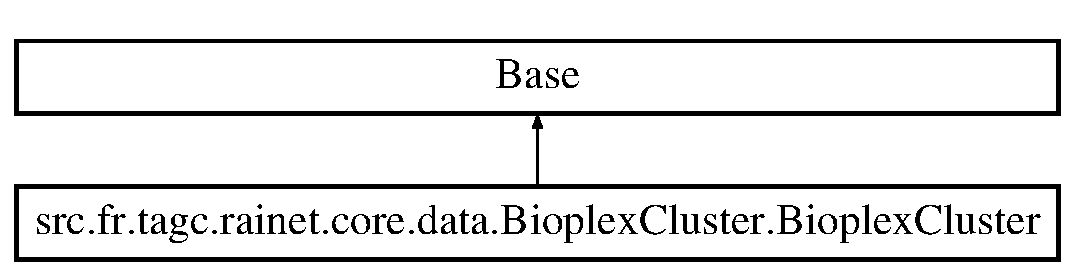
\includegraphics[height=2.000000cm]{classsrc_1_1fr_1_1tagc_1_1rainet_1_1core_1_1data_1_1BioplexCluster_1_1BioplexCluster}
\end{center}
\end{figure}
\subsection*{Public Member Functions}
\begin{DoxyCompactItemize}
\item 
\hypertarget{classsrc_1_1fr_1_1tagc_1_1rainet_1_1core_1_1data_1_1BioplexCluster_1_1BioplexCluster_a8174745122e8e54cedb0a0e5673426ad}{def {\bfseries \-\_\-\-\_\-init\-\_\-\-\_\-}}\label{classsrc_1_1fr_1_1tagc_1_1rainet_1_1core_1_1data_1_1BioplexCluster_1_1BioplexCluster_a8174745122e8e54cedb0a0e5673426ad}

\item 
\hypertarget{classsrc_1_1fr_1_1tagc_1_1rainet_1_1core_1_1data_1_1BioplexCluster_1_1BioplexCluster_aea5b415552809c0d6577ac4e80c0f533}{def \hyperlink{classsrc_1_1fr_1_1tagc_1_1rainet_1_1core_1_1data_1_1BioplexCluster_1_1BioplexCluster_aea5b415552809c0d6577ac4e80c0f533}{add\-\_\-to\-\_\-session}}\label{classsrc_1_1fr_1_1tagc_1_1rainet_1_1core_1_1data_1_1BioplexCluster_1_1BioplexCluster_aea5b415552809c0d6577ac4e80c0f533}

\begin{DoxyCompactList}\small\item\em Add the object to S\-Q\-L\-Alchemy session if it is linked to a protein. \end{DoxyCompactList}\item 
\hypertarget{classsrc_1_1fr_1_1tagc_1_1rainet_1_1core_1_1data_1_1BioplexCluster_1_1BioplexCluster_ac5b31e28e2336efb9a0c86a8c07b8cde}{def \hyperlink{classsrc_1_1fr_1_1tagc_1_1rainet_1_1core_1_1data_1_1BioplexCluster_1_1BioplexCluster_ac5b31e28e2336efb9a0c86a8c07b8cde}{add\-\_\-annotated\-\_\-protein}}\label{classsrc_1_1fr_1_1tagc_1_1rainet_1_1core_1_1data_1_1BioplexCluster_1_1BioplexCluster_ac5b31e28e2336efb9a0c86a8c07b8cde}

\begin{DoxyCompactList}\small\item\em Add an annotated protein to the list. \end{DoxyCompactList}\end{DoxyCompactItemize}
\subsection*{Public Attributes}
\begin{DoxyCompactItemize}
\item 
\hypertarget{classsrc_1_1fr_1_1tagc_1_1rainet_1_1core_1_1data_1_1BioplexCluster_1_1BioplexCluster_a9689dcaa3737024caa83f83a5f542948}{{\bfseries bioplex\-I\-D}}\label{classsrc_1_1fr_1_1tagc_1_1rainet_1_1core_1_1data_1_1BioplexCluster_1_1BioplexCluster_a9689dcaa3737024caa83f83a5f542948}

\end{DoxyCompactItemize}
\subsection*{Static Public Attributes}
\begin{DoxyCompactItemize}
\item 
\hypertarget{classsrc_1_1fr_1_1tagc_1_1rainet_1_1core_1_1data_1_1BioplexCluster_1_1BioplexCluster_a95ffebe7d3accdcd290ea925625c2efd}{tuple {\bfseries bioplex\-I\-D} = Column( String, primary\-\_\-key = True )}\label{classsrc_1_1fr_1_1tagc_1_1rainet_1_1core_1_1data_1_1BioplexCluster_1_1BioplexCluster_a95ffebe7d3accdcd290ea925625c2efd}

\item 
\hypertarget{classsrc_1_1fr_1_1tagc_1_1rainet_1_1core_1_1data_1_1BioplexCluster_1_1BioplexCluster_ad9caecab8849f2f56b097a91499fbac1}{tuple {\bfseries annotated\-Proteins} = relationship('Protein', secondary=Protein\-Bioplex\-Annotation.\-\_\-\-\_\-table\-\_\-\-\_\-, backref=\char`\"{}bioplex\-Annotations\char`\"{})}\label{classsrc_1_1fr_1_1tagc_1_1rainet_1_1core_1_1data_1_1BioplexCluster_1_1BioplexCluster_ad9caecab8849f2f56b097a91499fbac1}

\end{DoxyCompactItemize}


The documentation for this class was generated from the following file\-:\begin{DoxyCompactItemize}
\item 
src/fr/tagc/rainet/core/data/Bioplex\-Cluster.\-py\end{DoxyCompactItemize}

\hypertarget{classsrc_1_1core_1_1execution_1_1ClassificationNewDataset_1_1ClassificationNewDataset}{\section{src.\-core.\-execution.\-Classification\-New\-Dataset.\-Classification\-New\-Dataset Class Reference}
\label{classsrc_1_1core_1_1execution_1_1ClassificationNewDataset_1_1ClassificationNewDataset}\index{src.\-core.\-execution.\-Classification\-New\-Dataset.\-Classification\-New\-Dataset@{src.\-core.\-execution.\-Classification\-New\-Dataset.\-Classification\-New\-Dataset}}
}
\subsection*{Public Member Functions}
\begin{DoxyCompactItemize}
\item 
\hypertarget{classsrc_1_1core_1_1execution_1_1ClassificationNewDataset_1_1ClassificationNewDataset_a267b17ae3c80b399df841739fab8c1b2}{def {\bfseries mrna\-\_\-protein}}\label{classsrc_1_1core_1_1execution_1_1ClassificationNewDataset_1_1ClassificationNewDataset_a267b17ae3c80b399df841739fab8c1b2}

\item 
\hypertarget{classsrc_1_1core_1_1execution_1_1ClassificationNewDataset_1_1ClassificationNewDataset_acfb4f1d0ecae5a6c030329f6d0a1439d}{def {\bfseries rna\-\_\-target}}\label{classsrc_1_1core_1_1execution_1_1ClassificationNewDataset_1_1ClassificationNewDataset_acfb4f1d0ecae5a6c030329f6d0a1439d}

\item 
\hypertarget{classsrc_1_1core_1_1execution_1_1ClassificationNewDataset_1_1ClassificationNewDataset_a4d2c081c35737aba6b7dec2bdba37375}{def {\bfseries domain\-\_\-classification}}\label{classsrc_1_1core_1_1execution_1_1ClassificationNewDataset_1_1ClassificationNewDataset_a4d2c081c35737aba6b7dec2bdba37375}

\end{DoxyCompactItemize}
\subsection*{Public Attributes}
\begin{DoxyCompactItemize}
\item 
\hypertarget{classsrc_1_1core_1_1execution_1_1ClassificationNewDataset_1_1ClassificationNewDataset_afe1113d13d8ec55bd36d7015f1f442d2}{{\bfseries path\-\_\-home}}\label{classsrc_1_1core_1_1execution_1_1ClassificationNewDataset_1_1ClassificationNewDataset_afe1113d13d8ec55bd36d7015f1f442d2}

\item 
\hypertarget{classsrc_1_1core_1_1execution_1_1ClassificationNewDataset_1_1ClassificationNewDataset_a9afc14534af71191e82e9e3845083829}{{\bfseries jproteomics\-\_\-seq}}\label{classsrc_1_1core_1_1execution_1_1ClassificationNewDataset_1_1ClassificationNewDataset_a9afc14534af71191e82e9e3845083829}

\item 
\hypertarget{classsrc_1_1core_1_1execution_1_1ClassificationNewDataset_1_1ClassificationNewDataset_aecbcc4aedfea420a2fdcc1ebfef57ee6}{{\bfseries jproteomics\-\_\-info}}\label{classsrc_1_1core_1_1execution_1_1ClassificationNewDataset_1_1ClassificationNewDataset_aecbcc4aedfea420a2fdcc1ebfef57ee6}

\item 
\hypertarget{classsrc_1_1core_1_1execution_1_1ClassificationNewDataset_1_1ClassificationNewDataset_ac8c8783374a639cf49e3a09b7f00d5fe}{{\bfseries header}}\label{classsrc_1_1core_1_1execution_1_1ClassificationNewDataset_1_1ClassificationNewDataset_ac8c8783374a639cf49e3a09b7f00d5fe}

\item 
\hypertarget{classsrc_1_1core_1_1execution_1_1ClassificationNewDataset_1_1ClassificationNewDataset_a33b3ed7f9503583dafe8621cddfc13d1}{{\bfseries file\-\_\-rna\-\_\-target\-\_\-jeproteomics}}\label{classsrc_1_1core_1_1execution_1_1ClassificationNewDataset_1_1ClassificationNewDataset_a33b3ed7f9503583dafe8621cddfc13d1}

\item 
\hypertarget{classsrc_1_1core_1_1execution_1_1ClassificationNewDataset_1_1ClassificationNewDataset_abd7ec9647152b02fbfec7e109e5cbbe9}{{\bfseries file\-\_\-rbpdb\-\_\-jproteomics}}\label{classsrc_1_1core_1_1execution_1_1ClassificationNewDataset_1_1ClassificationNewDataset_abd7ec9647152b02fbfec7e109e5cbbe9}

\item 
\hypertarget{classsrc_1_1core_1_1execution_1_1ClassificationNewDataset_1_1ClassificationNewDataset_a1d0655d2514762b379d4f9153f7b2ec0}{{\bfseries file\-\_\-seq\-\_\-natrevgenetics}}\label{classsrc_1_1core_1_1execution_1_1ClassificationNewDataset_1_1ClassificationNewDataset_a1d0655d2514762b379d4f9153f7b2ec0}

\item 
\hypertarget{classsrc_1_1core_1_1execution_1_1ClassificationNewDataset_1_1ClassificationNewDataset_a9586967234e64eae84df67aceec492fd}{{\bfseries natrevgenetics\-\_\-info}}\label{classsrc_1_1core_1_1execution_1_1ClassificationNewDataset_1_1ClassificationNewDataset_a9586967234e64eae84df67aceec492fd}

\item 
\hypertarget{classsrc_1_1core_1_1execution_1_1ClassificationNewDataset_1_1ClassificationNewDataset_affdab082e8a812fd47ef1d9f64ca4651}{{\bfseries file\-\_\-all\-\_\-rna\-\_\-target}}\label{classsrc_1_1core_1_1execution_1_1ClassificationNewDataset_1_1ClassificationNewDataset_affdab082e8a812fd47ef1d9f64ca4651}

\item 
\hypertarget{classsrc_1_1core_1_1execution_1_1ClassificationNewDataset_1_1ClassificationNewDataset_a1310b89f677fe77b6e548a7bd3cc0151}{{\bfseries file\-\_\-domain}}\label{classsrc_1_1core_1_1execution_1_1ClassificationNewDataset_1_1ClassificationNewDataset_a1310b89f677fe77b6e548a7bd3cc0151}

\item 
\hypertarget{classsrc_1_1core_1_1execution_1_1ClassificationNewDataset_1_1ClassificationNewDataset_ab4a83fd7763f2f840dfefd869f8190cb}{{\bfseries file\-\_\-jprot\-\_\-information}}\label{classsrc_1_1core_1_1execution_1_1ClassificationNewDataset_1_1ClassificationNewDataset_ab4a83fd7763f2f840dfefd869f8190cb}

\item 
\hypertarget{classsrc_1_1core_1_1execution_1_1ClassificationNewDataset_1_1ClassificationNewDataset_a5c8cd3c8c14e3c3a84dfc2b4ee4c5013}{{\bfseries file\-\_\-pfamid}}\label{classsrc_1_1core_1_1execution_1_1ClassificationNewDataset_1_1ClassificationNewDataset_a5c8cd3c8c14e3c3a84dfc2b4ee4c5013}

\item 
\hypertarget{classsrc_1_1core_1_1execution_1_1ClassificationNewDataset_1_1ClassificationNewDataset_a1f69afc21059fe35a979f146ae9f82c7}{{\bfseries path\-\_\-ouput\-\_\-file\-\_\-jprot}}\label{classsrc_1_1core_1_1execution_1_1ClassificationNewDataset_1_1ClassificationNewDataset_a1f69afc21059fe35a979f146ae9f82c7}

\item 
\hypertarget{classsrc_1_1core_1_1execution_1_1ClassificationNewDataset_1_1ClassificationNewDataset_a0a795952c28c5df36cf4557e023290bf}{{\bfseries input\-\_\-file\-\_\-nrgenetics}}\label{classsrc_1_1core_1_1execution_1_1ClassificationNewDataset_1_1ClassificationNewDataset_a0a795952c28c5df36cf4557e023290bf}

\item 
\hypertarget{classsrc_1_1core_1_1execution_1_1ClassificationNewDataset_1_1ClassificationNewDataset_aff042a43fd25c9e79792888df6b109f3}{{\bfseries path\-\_\-ouput\-\_\-file\-\_\-nrgenetics}}\label{classsrc_1_1core_1_1execution_1_1ClassificationNewDataset_1_1ClassificationNewDataset_aff042a43fd25c9e79792888df6b109f3}

\item 
\hypertarget{classsrc_1_1core_1_1execution_1_1ClassificationNewDataset_1_1ClassificationNewDataset_a776de1a1ed2e4da85a4e438f5a42756d}{{\bfseries file\-\_\-sequences}}\label{classsrc_1_1core_1_1execution_1_1ClassificationNewDataset_1_1ClassificationNewDataset_a776de1a1ed2e4da85a4e438f5a42756d}

\item 
\hypertarget{classsrc_1_1core_1_1execution_1_1ClassificationNewDataset_1_1ClassificationNewDataset_aeed4cf4a8a65d67c4b1fec794248101d}{{\bfseries final\-\_\-file\-\_\-table}}\label{classsrc_1_1core_1_1execution_1_1ClassificationNewDataset_1_1ClassificationNewDataset_aeed4cf4a8a65d67c4b1fec794248101d}

\end{DoxyCompactItemize}


The documentation for this class was generated from the following file\-:\begin{DoxyCompactItemize}
\item 
rbp-\/motif/src/core/execution/Classification\-New\-Dataset.\-py\end{DoxyCompactItemize}

\hypertarget{classsrc_1_1fr_1_1tagc_1_1rainet_1_1core_1_1execution_1_1analysis_1_1EnrichmentAnalysis_1_1Commocb4af204a9dc077e1a18361d5afc6b0c}{\section{src.\-fr.\-tagc.\-rainet.\-core.\-execution.\-analysis.\-Enrichment\-Analysis.\-Common\-Lnc\-R\-N\-A\-Protein\-Disease.\-Common\-Lnc\-R\-N\-A\-Protein\-Disease Class Reference}
\label{classsrc_1_1fr_1_1tagc_1_1rainet_1_1core_1_1execution_1_1analysis_1_1EnrichmentAnalysis_1_1Commocb4af204a9dc077e1a18361d5afc6b0c}\index{src.\-fr.\-tagc.\-rainet.\-core.\-execution.\-analysis.\-Enrichment\-Analysis.\-Common\-Lnc\-R\-N\-A\-Protein\-Disease.\-Common\-Lnc\-R\-N\-A\-Protein\-Disease@{src.\-fr.\-tagc.\-rainet.\-core.\-execution.\-analysis.\-Enrichment\-Analysis.\-Common\-Lnc\-R\-N\-A\-Protein\-Disease.\-Common\-Lnc\-R\-N\-A\-Protein\-Disease}}
}
Inheritance diagram for src.\-fr.\-tagc.\-rainet.\-core.\-execution.\-analysis.\-Enrichment\-Analysis.\-Common\-Lnc\-R\-N\-A\-Protein\-Disease.\-Common\-Lnc\-R\-N\-A\-Protein\-Disease\-:\begin{figure}[H]
\begin{center}
\leavevmode
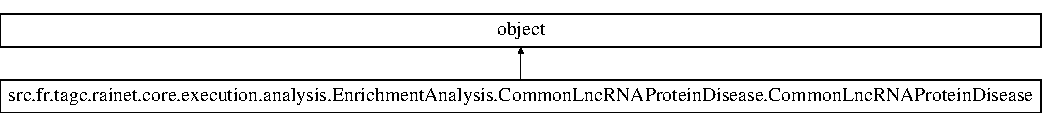
\includegraphics[height=1.521739cm]{classsrc_1_1fr_1_1tagc_1_1rainet_1_1core_1_1execution_1_1analysis_1_1EnrichmentAnalysis_1_1Commocb4af204a9dc077e1a18361d5afc6b0c}
\end{center}
\end{figure}
\subsection*{Public Member Functions}
\begin{DoxyCompactItemize}
\item 
\hypertarget{classsrc_1_1fr_1_1tagc_1_1rainet_1_1core_1_1execution_1_1analysis_1_1EnrichmentAnalysis_1_1Commocb4af204a9dc077e1a18361d5afc6b0c_a446edee017f3fd6640309c373a262fdf}{def {\bfseries \-\_\-\-\_\-init\-\_\-\-\_\-}}\label{classsrc_1_1fr_1_1tagc_1_1rainet_1_1core_1_1execution_1_1analysis_1_1EnrichmentAnalysis_1_1Commocb4af204a9dc077e1a18361d5afc6b0c_a446edee017f3fd6640309c373a262fdf}

\item 
\hypertarget{classsrc_1_1fr_1_1tagc_1_1rainet_1_1core_1_1execution_1_1analysis_1_1EnrichmentAnalysis_1_1Commocb4af204a9dc077e1a18361d5afc6b0c_a78d1249539d3a7bb9809ee53b484f0be}{def {\bfseries read\-\_\-rainet\-\_\-db}}\label{classsrc_1_1fr_1_1tagc_1_1rainet_1_1core_1_1execution_1_1analysis_1_1EnrichmentAnalysis_1_1Commocb4af204a9dc077e1a18361d5afc6b0c_a78d1249539d3a7bb9809ee53b484f0be}

\item 
\hypertarget{classsrc_1_1fr_1_1tagc_1_1rainet_1_1core_1_1execution_1_1analysis_1_1EnrichmentAnalysis_1_1Commocb4af204a9dc077e1a18361d5afc6b0c_a2f8564bff3cc9a7aa06121f5defaf66d}{def {\bfseries read\-\_\-black\-\_\-listed\-\_\-words\-\_\-file}}\label{classsrc_1_1fr_1_1tagc_1_1rainet_1_1core_1_1execution_1_1analysis_1_1EnrichmentAnalysis_1_1Commocb4af204a9dc077e1a18361d5afc6b0c_a2f8564bff3cc9a7aa06121f5defaf66d}

\item 
\hypertarget{classsrc_1_1fr_1_1tagc_1_1rainet_1_1core_1_1execution_1_1analysis_1_1EnrichmentAnalysis_1_1Commocb4af204a9dc077e1a18361d5afc6b0c_a7c5aba5b3fcef9b13bc15cfe2057532d}{def {\bfseries read\-\_\-lncrna\-\_\-disease\-\_\-file}}\label{classsrc_1_1fr_1_1tagc_1_1rainet_1_1core_1_1execution_1_1analysis_1_1EnrichmentAnalysis_1_1Commocb4af204a9dc077e1a18361d5afc6b0c_a7c5aba5b3fcef9b13bc15cfe2057532d}

\item 
\hypertarget{classsrc_1_1fr_1_1tagc_1_1rainet_1_1core_1_1execution_1_1analysis_1_1EnrichmentAnalysis_1_1Commocb4af204a9dc077e1a18361d5afc6b0c_a5195528c7cb2595c205b142794f8e02b}{def {\bfseries read\-\_\-protein\-\_\-disease\-\_\-file}}\label{classsrc_1_1fr_1_1tagc_1_1rainet_1_1core_1_1execution_1_1analysis_1_1EnrichmentAnalysis_1_1Commocb4af204a9dc077e1a18361d5afc6b0c_a5195528c7cb2595c205b142794f8e02b}

\item 
\hypertarget{classsrc_1_1fr_1_1tagc_1_1rainet_1_1core_1_1execution_1_1analysis_1_1EnrichmentAnalysis_1_1Commocb4af204a9dc077e1a18361d5afc6b0c_a594f90c3dfb5cb0167e6df4039501fdc}{def {\bfseries enrichment\-\_\-to\-\_\-protein}}\label{classsrc_1_1fr_1_1tagc_1_1rainet_1_1core_1_1execution_1_1analysis_1_1EnrichmentAnalysis_1_1Commocb4af204a9dc077e1a18361d5afc6b0c_a594f90c3dfb5cb0167e6df4039501fdc}

\item 
\hypertarget{classsrc_1_1fr_1_1tagc_1_1rainet_1_1core_1_1execution_1_1analysis_1_1EnrichmentAnalysis_1_1Commocb4af204a9dc077e1a18361d5afc6b0c_a586bdb7528c77e71141c6a6145b365eb}{def {\bfseries process\-\_\-lncrna\-\_\-protein\-\_\-map}}\label{classsrc_1_1fr_1_1tagc_1_1rainet_1_1core_1_1execution_1_1analysis_1_1EnrichmentAnalysis_1_1Commocb4af204a9dc077e1a18361d5afc6b0c_a586bdb7528c77e71141c6a6145b365eb}

\item 
\hypertarget{classsrc_1_1fr_1_1tagc_1_1rainet_1_1core_1_1execution_1_1analysis_1_1EnrichmentAnalysis_1_1Commocb4af204a9dc077e1a18361d5afc6b0c_ad7837ae8ee15c2a2d90a612bebc6876b}{def {\bfseries run}}\label{classsrc_1_1fr_1_1tagc_1_1rainet_1_1core_1_1execution_1_1analysis_1_1EnrichmentAnalysis_1_1Commocb4af204a9dc077e1a18361d5afc6b0c_ad7837ae8ee15c2a2d90a612bebc6876b}

\end{DoxyCompactItemize}
\subsection*{Public Attributes}
\begin{DoxyCompactItemize}
\item 
\hypertarget{classsrc_1_1fr_1_1tagc_1_1rainet_1_1core_1_1execution_1_1analysis_1_1EnrichmentAnalysis_1_1Commocb4af204a9dc077e1a18361d5afc6b0c_a0d29fec0c47d3092e90a2a439d95ff96}{{\bfseries rainet\-D\-B}}\label{classsrc_1_1fr_1_1tagc_1_1rainet_1_1core_1_1execution_1_1analysis_1_1EnrichmentAnalysis_1_1Commocb4af204a9dc077e1a18361d5afc6b0c_a0d29fec0c47d3092e90a2a439d95ff96}

\item 
\hypertarget{classsrc_1_1fr_1_1tagc_1_1rainet_1_1core_1_1execution_1_1analysis_1_1EnrichmentAnalysis_1_1Commocb4af204a9dc077e1a18361d5afc6b0c_a954c354a903d53ba9c1aca480934bfcc}{{\bfseries lnc\-R\-N\-A\-Disease\-File}}\label{classsrc_1_1fr_1_1tagc_1_1rainet_1_1core_1_1execution_1_1analysis_1_1EnrichmentAnalysis_1_1Commocb4af204a9dc077e1a18361d5afc6b0c_a954c354a903d53ba9c1aca480934bfcc}

\item 
\hypertarget{classsrc_1_1fr_1_1tagc_1_1rainet_1_1core_1_1execution_1_1analysis_1_1EnrichmentAnalysis_1_1Commocb4af204a9dc077e1a18361d5afc6b0c_a8ff8dc47dd7d4beadeddbd94b555e5a0}{{\bfseries protein\-Disease\-File}}\label{classsrc_1_1fr_1_1tagc_1_1rainet_1_1core_1_1execution_1_1analysis_1_1EnrichmentAnalysis_1_1Commocb4af204a9dc077e1a18361d5afc6b0c_a8ff8dc47dd7d4beadeddbd94b555e5a0}

\item 
\hypertarget{classsrc_1_1fr_1_1tagc_1_1rainet_1_1core_1_1execution_1_1analysis_1_1EnrichmentAnalysis_1_1Commocb4af204a9dc077e1a18361d5afc6b0c_a3dbf8774789f68602114648da43c5252}{{\bfseries enrichment\-Data}}\label{classsrc_1_1fr_1_1tagc_1_1rainet_1_1core_1_1execution_1_1analysis_1_1EnrichmentAnalysis_1_1Commocb4af204a9dc077e1a18361d5afc6b0c_a3dbf8774789f68602114648da43c5252}

\item 
\hypertarget{classsrc_1_1fr_1_1tagc_1_1rainet_1_1core_1_1execution_1_1analysis_1_1EnrichmentAnalysis_1_1Commocb4af204a9dc077e1a18361d5afc6b0c_a2590ea7cba8e58e644f1509c5ed2bf33}{{\bfseries output\-Folder}}\label{classsrc_1_1fr_1_1tagc_1_1rainet_1_1core_1_1execution_1_1analysis_1_1EnrichmentAnalysis_1_1Commocb4af204a9dc077e1a18361d5afc6b0c_a2590ea7cba8e58e644f1509c5ed2bf33}

\item 
\hypertarget{classsrc_1_1fr_1_1tagc_1_1rainet_1_1core_1_1execution_1_1analysis_1_1EnrichmentAnalysis_1_1Commocb4af204a9dc077e1a18361d5afc6b0c_a6224b5e2f1eef9a9e3e86fad28cecebe}{{\bfseries min\-Word\-Size}}\label{classsrc_1_1fr_1_1tagc_1_1rainet_1_1core_1_1execution_1_1analysis_1_1EnrichmentAnalysis_1_1Commocb4af204a9dc077e1a18361d5afc6b0c_a6224b5e2f1eef9a9e3e86fad28cecebe}

\item 
\hypertarget{classsrc_1_1fr_1_1tagc_1_1rainet_1_1core_1_1execution_1_1analysis_1_1EnrichmentAnalysis_1_1Commocb4af204a9dc077e1a18361d5afc6b0c_a9f79d820b62dc1c03403d42648145757}{{\bfseries black\-Listed\-Words}}\label{classsrc_1_1fr_1_1tagc_1_1rainet_1_1core_1_1execution_1_1analysis_1_1EnrichmentAnalysis_1_1Commocb4af204a9dc077e1a18361d5afc6b0c_a9f79d820b62dc1c03403d42648145757}

\item 
\hypertarget{classsrc_1_1fr_1_1tagc_1_1rainet_1_1core_1_1execution_1_1analysis_1_1EnrichmentAnalysis_1_1Commocb4af204a9dc077e1a18361d5afc6b0c_a8bc9c83a43093255736cfdc8b8b24387}{{\bfseries complex\-Datasets}}\label{classsrc_1_1fr_1_1tagc_1_1rainet_1_1core_1_1execution_1_1analysis_1_1EnrichmentAnalysis_1_1Commocb4af204a9dc077e1a18361d5afc6b0c_a8bc9c83a43093255736cfdc8b8b24387}

\item 
\hypertarget{classsrc_1_1fr_1_1tagc_1_1rainet_1_1core_1_1execution_1_1analysis_1_1EnrichmentAnalysis_1_1Commocb4af204a9dc077e1a18361d5afc6b0c_a37fa65dd838e27c979b013695afeab0b}{{\bfseries black\-Listed\-Words\-Set}}\label{classsrc_1_1fr_1_1tagc_1_1rainet_1_1core_1_1execution_1_1analysis_1_1EnrichmentAnalysis_1_1Commocb4af204a9dc077e1a18361d5afc6b0c_a37fa65dd838e27c979b013695afeab0b}

\item 
\hypertarget{classsrc_1_1fr_1_1tagc_1_1rainet_1_1core_1_1execution_1_1analysis_1_1EnrichmentAnalysis_1_1Commocb4af204a9dc077e1a18361d5afc6b0c_a46eb04883d57d8dee76c1a2907c4fadd}{{\bfseries sql\-\_\-session}}\label{classsrc_1_1fr_1_1tagc_1_1rainet_1_1core_1_1execution_1_1analysis_1_1EnrichmentAnalysis_1_1Commocb4af204a9dc077e1a18361d5afc6b0c_a46eb04883d57d8dee76c1a2907c4fadd}

\item 
\hypertarget{classsrc_1_1fr_1_1tagc_1_1rainet_1_1core_1_1execution_1_1analysis_1_1EnrichmentAnalysis_1_1Commocb4af204a9dc077e1a18361d5afc6b0c_a5617dce767eacb43dbe7c866299ee7cc}{{\bfseries transcript\-Interaction\-Dict}}\label{classsrc_1_1fr_1_1tagc_1_1rainet_1_1core_1_1execution_1_1analysis_1_1EnrichmentAnalysis_1_1Commocb4af204a9dc077e1a18361d5afc6b0c_a5617dce767eacb43dbe7c866299ee7cc}

\item 
\hypertarget{classsrc_1_1fr_1_1tagc_1_1rainet_1_1core_1_1execution_1_1analysis_1_1EnrichmentAnalysis_1_1Commocb4af204a9dc077e1a18361d5afc6b0c_a01ba9f2c3c2d4d9fcd2c20052142022c}{{\bfseries gene\-Transcript\-Dict}}\label{classsrc_1_1fr_1_1tagc_1_1rainet_1_1core_1_1execution_1_1analysis_1_1EnrichmentAnalysis_1_1Commocb4af204a9dc077e1a18361d5afc6b0c_a01ba9f2c3c2d4d9fcd2c20052142022c}

\item 
\hypertarget{classsrc_1_1fr_1_1tagc_1_1rainet_1_1core_1_1execution_1_1analysis_1_1EnrichmentAnalysis_1_1Commocb4af204a9dc077e1a18361d5afc6b0c_ae9fbd1b3cf1253d61a1274e96e68f4c7}{{\bfseries transcript\-Disease\-Dict}}\label{classsrc_1_1fr_1_1tagc_1_1rainet_1_1core_1_1execution_1_1analysis_1_1EnrichmentAnalysis_1_1Commocb4af204a9dc077e1a18361d5afc6b0c_ae9fbd1b3cf1253d61a1274e96e68f4c7}

\item 
\hypertarget{classsrc_1_1fr_1_1tagc_1_1rainet_1_1core_1_1execution_1_1analysis_1_1EnrichmentAnalysis_1_1Commocb4af204a9dc077e1a18361d5afc6b0c_ae636f05346dd1d71ce14d56898b5422e}{{\bfseries protein\-Disease\-Dict}}\label{classsrc_1_1fr_1_1tagc_1_1rainet_1_1core_1_1execution_1_1analysis_1_1EnrichmentAnalysis_1_1Commocb4af204a9dc077e1a18361d5afc6b0c_ae636f05346dd1d71ce14d56898b5422e}

\item 
\hypertarget{classsrc_1_1fr_1_1tagc_1_1rainet_1_1core_1_1execution_1_1analysis_1_1EnrichmentAnalysis_1_1Commocb4af204a9dc077e1a18361d5afc6b0c_a4d97af453f561c1199da653139fd15bf}{{\bfseries pairs\-To\-Write}}\label{classsrc_1_1fr_1_1tagc_1_1rainet_1_1core_1_1execution_1_1analysis_1_1EnrichmentAnalysis_1_1Commocb4af204a9dc077e1a18361d5afc6b0c_a4d97af453f561c1199da653139fd15bf}

\item 
\hypertarget{classsrc_1_1fr_1_1tagc_1_1rainet_1_1core_1_1execution_1_1analysis_1_1EnrichmentAnalysis_1_1Commocb4af204a9dc077e1a18361d5afc6b0c_ae0ff0088feb1262f324ee2e9e0a326bb}{{\bfseries enrichments\-Dict}}\label{classsrc_1_1fr_1_1tagc_1_1rainet_1_1core_1_1execution_1_1analysis_1_1EnrichmentAnalysis_1_1Commocb4af204a9dc077e1a18361d5afc6b0c_ae0ff0088feb1262f324ee2e9e0a326bb}

\end{DoxyCompactItemize}
\subsection*{Static Public Attributes}
\begin{DoxyCompactItemize}
\item 
\hypertarget{classsrc_1_1fr_1_1tagc_1_1rainet_1_1core_1_1execution_1_1analysis_1_1EnrichmentAnalysis_1_1Commocb4af204a9dc077e1a18361d5afc6b0c_a72f2d2ec6b36f3ff0f37d098395c8924}{string {\bfseries O\-U\-T\-P\-U\-T\-\_\-\-F\-I\-L\-E\-\_\-\-W\-O\-R\-D\-\_\-\-M\-A\-T\-C\-H} = \char`\"{}/lnc\-R\-N\-A\-\_\-protein\-\_\-disease\-\_\-descriptions\-\_\-word\-\_\-match.\-txt\char`\"{}}\label{classsrc_1_1fr_1_1tagc_1_1rainet_1_1core_1_1execution_1_1analysis_1_1EnrichmentAnalysis_1_1Commocb4af204a9dc077e1a18361d5afc6b0c_a72f2d2ec6b36f3ff0f37d098395c8924}

\end{DoxyCompactItemize}


The documentation for this class was generated from the following file\-:\begin{DoxyCompactItemize}
\item 
src/fr/tagc/rainet/core/execution/analysis/\-Enrichment\-Analysis/Common\-Lnc\-R\-N\-A\-Protein\-Disease.\-py\end{DoxyCompactItemize}

\hypertarget{classsrc_1_1fr_1_1tagc_1_1rainet_1_1core_1_1execution_1_1analysis_1_1EnrichmentAnalysis_1_1Commo70ca5c91857cc3a649e8e2158b3a9c9f}{\section{src.\-fr.\-tagc.\-rainet.\-core.\-execution.\-analysis.\-Enrichment\-Analysis.\-Common\-Lnc\-R\-N\-A\-Protein\-Disease2.\-Common\-Lnc\-R\-N\-A\-Protein\-Disease Class Reference}
\label{classsrc_1_1fr_1_1tagc_1_1rainet_1_1core_1_1execution_1_1analysis_1_1EnrichmentAnalysis_1_1Commo70ca5c91857cc3a649e8e2158b3a9c9f}\index{src.\-fr.\-tagc.\-rainet.\-core.\-execution.\-analysis.\-Enrichment\-Analysis.\-Common\-Lnc\-R\-N\-A\-Protein\-Disease2.\-Common\-Lnc\-R\-N\-A\-Protein\-Disease@{src.\-fr.\-tagc.\-rainet.\-core.\-execution.\-analysis.\-Enrichment\-Analysis.\-Common\-Lnc\-R\-N\-A\-Protein\-Disease2.\-Common\-Lnc\-R\-N\-A\-Protein\-Disease}}
}
Inheritance diagram for src.\-fr.\-tagc.\-rainet.\-core.\-execution.\-analysis.\-Enrichment\-Analysis.\-Common\-Lnc\-R\-N\-A\-Protein\-Disease2.\-Common\-Lnc\-R\-N\-A\-Protein\-Disease\-:\begin{figure}[H]
\begin{center}
\leavevmode
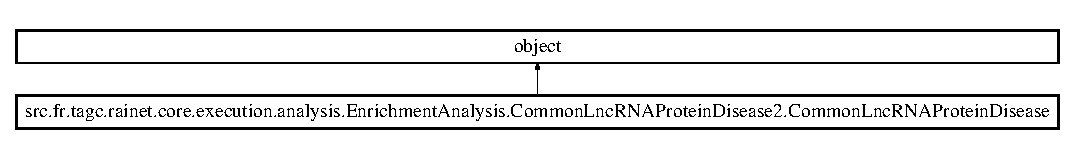
\includegraphics[height=1.507402cm]{classsrc_1_1fr_1_1tagc_1_1rainet_1_1core_1_1execution_1_1analysis_1_1EnrichmentAnalysis_1_1Commo70ca5c91857cc3a649e8e2158b3a9c9f}
\end{center}
\end{figure}
\subsection*{Public Member Functions}
\begin{DoxyCompactItemize}
\item 
\hypertarget{classsrc_1_1fr_1_1tagc_1_1rainet_1_1core_1_1execution_1_1analysis_1_1EnrichmentAnalysis_1_1Commo70ca5c91857cc3a649e8e2158b3a9c9f_abe28bbe72cb6f30cb512ad186376fa19}{def {\bfseries \-\_\-\-\_\-init\-\_\-\-\_\-}}\label{classsrc_1_1fr_1_1tagc_1_1rainet_1_1core_1_1execution_1_1analysis_1_1EnrichmentAnalysis_1_1Commo70ca5c91857cc3a649e8e2158b3a9c9f_abe28bbe72cb6f30cb512ad186376fa19}

\item 
\hypertarget{classsrc_1_1fr_1_1tagc_1_1rainet_1_1core_1_1execution_1_1analysis_1_1EnrichmentAnalysis_1_1Commo70ca5c91857cc3a649e8e2158b3a9c9f_acee5b184166a556e5ddefd618e5286d0}{def {\bfseries read\-\_\-rainet\-\_\-db}}\label{classsrc_1_1fr_1_1tagc_1_1rainet_1_1core_1_1execution_1_1analysis_1_1EnrichmentAnalysis_1_1Commo70ca5c91857cc3a649e8e2158b3a9c9f_acee5b184166a556e5ddefd618e5286d0}

\item 
\hypertarget{classsrc_1_1fr_1_1tagc_1_1rainet_1_1core_1_1execution_1_1analysis_1_1EnrichmentAnalysis_1_1Commo70ca5c91857cc3a649e8e2158b3a9c9f_a63f1c4cc0a3cffcb77b539ea1227be48}{def {\bfseries read\-\_\-black\-\_\-listed\-\_\-words\-\_\-file}}\label{classsrc_1_1fr_1_1tagc_1_1rainet_1_1core_1_1execution_1_1analysis_1_1EnrichmentAnalysis_1_1Commo70ca5c91857cc3a649e8e2158b3a9c9f_a63f1c4cc0a3cffcb77b539ea1227be48}

\item 
\hypertarget{classsrc_1_1fr_1_1tagc_1_1rainet_1_1core_1_1execution_1_1analysis_1_1EnrichmentAnalysis_1_1Commo70ca5c91857cc3a649e8e2158b3a9c9f_a32e502f07a5532a6745ab60bb4abe54e}{def {\bfseries read\-\_\-lncrna\-\_\-disease\-\_\-file}}\label{classsrc_1_1fr_1_1tagc_1_1rainet_1_1core_1_1execution_1_1analysis_1_1EnrichmentAnalysis_1_1Commo70ca5c91857cc3a649e8e2158b3a9c9f_a32e502f07a5532a6745ab60bb4abe54e}

\item 
\hypertarget{classsrc_1_1fr_1_1tagc_1_1rainet_1_1core_1_1execution_1_1analysis_1_1EnrichmentAnalysis_1_1Commo70ca5c91857cc3a649e8e2158b3a9c9f_aca17e56c87f435c38436881e2c0fd225}{def {\bfseries read\-\_\-protein\-\_\-disease\-\_\-file}}\label{classsrc_1_1fr_1_1tagc_1_1rainet_1_1core_1_1execution_1_1analysis_1_1EnrichmentAnalysis_1_1Commo70ca5c91857cc3a649e8e2158b3a9c9f_aca17e56c87f435c38436881e2c0fd225}

\item 
\hypertarget{classsrc_1_1fr_1_1tagc_1_1rainet_1_1core_1_1execution_1_1analysis_1_1EnrichmentAnalysis_1_1Commo70ca5c91857cc3a649e8e2158b3a9c9f_a89902227ca9df6b320aeff8d9d8c9a9d}{def {\bfseries enrichment\-\_\-to\-\_\-protein}}\label{classsrc_1_1fr_1_1tagc_1_1rainet_1_1core_1_1execution_1_1analysis_1_1EnrichmentAnalysis_1_1Commo70ca5c91857cc3a649e8e2158b3a9c9f_a89902227ca9df6b320aeff8d9d8c9a9d}

\item 
\hypertarget{classsrc_1_1fr_1_1tagc_1_1rainet_1_1core_1_1execution_1_1analysis_1_1EnrichmentAnalysis_1_1Commo70ca5c91857cc3a649e8e2158b3a9c9f_aaf9054c963c41f79908df106f245017d}{def {\bfseries process\-\_\-lncrna\-\_\-protein\-\_\-map}}\label{classsrc_1_1fr_1_1tagc_1_1rainet_1_1core_1_1execution_1_1analysis_1_1EnrichmentAnalysis_1_1Commo70ca5c91857cc3a649e8e2158b3a9c9f_aaf9054c963c41f79908df106f245017d}

\item 
\hypertarget{classsrc_1_1fr_1_1tagc_1_1rainet_1_1core_1_1execution_1_1analysis_1_1EnrichmentAnalysis_1_1Commo70ca5c91857cc3a649e8e2158b3a9c9f_abe47d2be2b5e396107934ab26946123d}{def {\bfseries run}}\label{classsrc_1_1fr_1_1tagc_1_1rainet_1_1core_1_1execution_1_1analysis_1_1EnrichmentAnalysis_1_1Commo70ca5c91857cc3a649e8e2158b3a9c9f_abe47d2be2b5e396107934ab26946123d}

\end{DoxyCompactItemize}
\subsection*{Public Attributes}
\begin{DoxyCompactItemize}
\item 
\hypertarget{classsrc_1_1fr_1_1tagc_1_1rainet_1_1core_1_1execution_1_1analysis_1_1EnrichmentAnalysis_1_1Commo70ca5c91857cc3a649e8e2158b3a9c9f_a0f534a070ecaadcf13a96f0de2528179}{{\bfseries rainet\-D\-B}}\label{classsrc_1_1fr_1_1tagc_1_1rainet_1_1core_1_1execution_1_1analysis_1_1EnrichmentAnalysis_1_1Commo70ca5c91857cc3a649e8e2158b3a9c9f_a0f534a070ecaadcf13a96f0de2528179}

\item 
\hypertarget{classsrc_1_1fr_1_1tagc_1_1rainet_1_1core_1_1execution_1_1analysis_1_1EnrichmentAnalysis_1_1Commo70ca5c91857cc3a649e8e2158b3a9c9f_a9158e5bf9dc52b185465037a523154ce}{{\bfseries lnc\-R\-N\-A\-Disease\-File}}\label{classsrc_1_1fr_1_1tagc_1_1rainet_1_1core_1_1execution_1_1analysis_1_1EnrichmentAnalysis_1_1Commo70ca5c91857cc3a649e8e2158b3a9c9f_a9158e5bf9dc52b185465037a523154ce}

\item 
\hypertarget{classsrc_1_1fr_1_1tagc_1_1rainet_1_1core_1_1execution_1_1analysis_1_1EnrichmentAnalysis_1_1Commo70ca5c91857cc3a649e8e2158b3a9c9f_a0814f9f1f82c42e0749933d2ab4ee6d1}{{\bfseries protein\-Disease\-File}}\label{classsrc_1_1fr_1_1tagc_1_1rainet_1_1core_1_1execution_1_1analysis_1_1EnrichmentAnalysis_1_1Commo70ca5c91857cc3a649e8e2158b3a9c9f_a0814f9f1f82c42e0749933d2ab4ee6d1}

\item 
\hypertarget{classsrc_1_1fr_1_1tagc_1_1rainet_1_1core_1_1execution_1_1analysis_1_1EnrichmentAnalysis_1_1Commo70ca5c91857cc3a649e8e2158b3a9c9f_a849604d686fa5ca0cbec656d07d2651c}{{\bfseries enrichment\-Data}}\label{classsrc_1_1fr_1_1tagc_1_1rainet_1_1core_1_1execution_1_1analysis_1_1EnrichmentAnalysis_1_1Commo70ca5c91857cc3a649e8e2158b3a9c9f_a849604d686fa5ca0cbec656d07d2651c}

\item 
\hypertarget{classsrc_1_1fr_1_1tagc_1_1rainet_1_1core_1_1execution_1_1analysis_1_1EnrichmentAnalysis_1_1Commo70ca5c91857cc3a649e8e2158b3a9c9f_a34ab9a48b674eaea8a3abce9c202cd5a}{{\bfseries output\-Folder}}\label{classsrc_1_1fr_1_1tagc_1_1rainet_1_1core_1_1execution_1_1analysis_1_1EnrichmentAnalysis_1_1Commo70ca5c91857cc3a649e8e2158b3a9c9f_a34ab9a48b674eaea8a3abce9c202cd5a}

\item 
\hypertarget{classsrc_1_1fr_1_1tagc_1_1rainet_1_1core_1_1execution_1_1analysis_1_1EnrichmentAnalysis_1_1Commo70ca5c91857cc3a649e8e2158b3a9c9f_a5d9a5007fa1a86ce3558437d3b594bef}{{\bfseries min\-Word\-Size}}\label{classsrc_1_1fr_1_1tagc_1_1rainet_1_1core_1_1execution_1_1analysis_1_1EnrichmentAnalysis_1_1Commo70ca5c91857cc3a649e8e2158b3a9c9f_a5d9a5007fa1a86ce3558437d3b594bef}

\item 
\hypertarget{classsrc_1_1fr_1_1tagc_1_1rainet_1_1core_1_1execution_1_1analysis_1_1EnrichmentAnalysis_1_1Commo70ca5c91857cc3a649e8e2158b3a9c9f_a1792cf6e2f2e980dfcf645449fc22bce}{{\bfseries black\-Listed\-Words}}\label{classsrc_1_1fr_1_1tagc_1_1rainet_1_1core_1_1execution_1_1analysis_1_1EnrichmentAnalysis_1_1Commo70ca5c91857cc3a649e8e2158b3a9c9f_a1792cf6e2f2e980dfcf645449fc22bce}

\item 
\hypertarget{classsrc_1_1fr_1_1tagc_1_1rainet_1_1core_1_1execution_1_1analysis_1_1EnrichmentAnalysis_1_1Commo70ca5c91857cc3a649e8e2158b3a9c9f_aa87ed7a0a317b796f9943172846f39cd}{{\bfseries complex\-Datasets}}\label{classsrc_1_1fr_1_1tagc_1_1rainet_1_1core_1_1execution_1_1analysis_1_1EnrichmentAnalysis_1_1Commo70ca5c91857cc3a649e8e2158b3a9c9f_aa87ed7a0a317b796f9943172846f39cd}

\item 
\hypertarget{classsrc_1_1fr_1_1tagc_1_1rainet_1_1core_1_1execution_1_1analysis_1_1EnrichmentAnalysis_1_1Commo70ca5c91857cc3a649e8e2158b3a9c9f_a757129e39c8907c93dcb5e7245cb713e}{{\bfseries black\-Listed\-Words\-Set}}\label{classsrc_1_1fr_1_1tagc_1_1rainet_1_1core_1_1execution_1_1analysis_1_1EnrichmentAnalysis_1_1Commo70ca5c91857cc3a649e8e2158b3a9c9f_a757129e39c8907c93dcb5e7245cb713e}

\item 
\hypertarget{classsrc_1_1fr_1_1tagc_1_1rainet_1_1core_1_1execution_1_1analysis_1_1EnrichmentAnalysis_1_1Commo70ca5c91857cc3a649e8e2158b3a9c9f_ab1a14e7ade6c74fd751b37080c1cb064}{{\bfseries sql\-\_\-session}}\label{classsrc_1_1fr_1_1tagc_1_1rainet_1_1core_1_1execution_1_1analysis_1_1EnrichmentAnalysis_1_1Commo70ca5c91857cc3a649e8e2158b3a9c9f_ab1a14e7ade6c74fd751b37080c1cb064}

\item 
\hypertarget{classsrc_1_1fr_1_1tagc_1_1rainet_1_1core_1_1execution_1_1analysis_1_1EnrichmentAnalysis_1_1Commo70ca5c91857cc3a649e8e2158b3a9c9f_a077ac2b32d19b9c0198db9ce91d7a970}{{\bfseries transcript\-Interaction\-Dict}}\label{classsrc_1_1fr_1_1tagc_1_1rainet_1_1core_1_1execution_1_1analysis_1_1EnrichmentAnalysis_1_1Commo70ca5c91857cc3a649e8e2158b3a9c9f_a077ac2b32d19b9c0198db9ce91d7a970}

\item 
\hypertarget{classsrc_1_1fr_1_1tagc_1_1rainet_1_1core_1_1execution_1_1analysis_1_1EnrichmentAnalysis_1_1Commo70ca5c91857cc3a649e8e2158b3a9c9f_a53689a00a0164920e25486cb17788c3c}{{\bfseries gene\-Transcript\-Dict}}\label{classsrc_1_1fr_1_1tagc_1_1rainet_1_1core_1_1execution_1_1analysis_1_1EnrichmentAnalysis_1_1Commo70ca5c91857cc3a649e8e2158b3a9c9f_a53689a00a0164920e25486cb17788c3c}

\item 
\hypertarget{classsrc_1_1fr_1_1tagc_1_1rainet_1_1core_1_1execution_1_1analysis_1_1EnrichmentAnalysis_1_1Commo70ca5c91857cc3a649e8e2158b3a9c9f_a977da760cc1dbe9fe0b73f5041b8982c}{{\bfseries transcript\-Disease\-Dict}}\label{classsrc_1_1fr_1_1tagc_1_1rainet_1_1core_1_1execution_1_1analysis_1_1EnrichmentAnalysis_1_1Commo70ca5c91857cc3a649e8e2158b3a9c9f_a977da760cc1dbe9fe0b73f5041b8982c}

\item 
\hypertarget{classsrc_1_1fr_1_1tagc_1_1rainet_1_1core_1_1execution_1_1analysis_1_1EnrichmentAnalysis_1_1Commo70ca5c91857cc3a649e8e2158b3a9c9f_a03b474fc82aee16b0aa31f92b900b2c0}{{\bfseries protein\-Disease\-Dict}}\label{classsrc_1_1fr_1_1tagc_1_1rainet_1_1core_1_1execution_1_1analysis_1_1EnrichmentAnalysis_1_1Commo70ca5c91857cc3a649e8e2158b3a9c9f_a03b474fc82aee16b0aa31f92b900b2c0}

\item 
\hyperlink{classsrc_1_1fr_1_1tagc_1_1rainet_1_1core_1_1execution_1_1analysis_1_1EnrichmentAnalysis_1_1Commo70ca5c91857cc3a649e8e2158b3a9c9f_a26d410f4b6627c31f1f3d1d77a896646}{pairs\-To\-Write}
\begin{DoxyCompactList}\small\item\em 30-\/\-May-\/2017 Add on to write a specific file for paper submission. \end{DoxyCompactList}\item 
\hypertarget{classsrc_1_1fr_1_1tagc_1_1rainet_1_1core_1_1execution_1_1analysis_1_1EnrichmentAnalysis_1_1Commo70ca5c91857cc3a649e8e2158b3a9c9f_a1f42fc8da1cab18b7f5e134870e33bba}{{\bfseries enrichments\-Dict}}\label{classsrc_1_1fr_1_1tagc_1_1rainet_1_1core_1_1execution_1_1analysis_1_1EnrichmentAnalysis_1_1Commo70ca5c91857cc3a649e8e2158b3a9c9f_a1f42fc8da1cab18b7f5e134870e33bba}

\end{DoxyCompactItemize}
\subsection*{Static Public Attributes}
\begin{DoxyCompactItemize}
\item 
\hypertarget{classsrc_1_1fr_1_1tagc_1_1rainet_1_1core_1_1execution_1_1analysis_1_1EnrichmentAnalysis_1_1Commo70ca5c91857cc3a649e8e2158b3a9c9f_a1128749d172d966deb7eef3bc0abc9e3}{string {\bfseries O\-U\-T\-P\-U\-T\-\_\-\-F\-I\-L\-E\-\_\-\-W\-O\-R\-D\-\_\-\-M\-A\-T\-C\-H} = \char`\"{}/lnc\-R\-N\-A\-\_\-protein\-\_\-disease\-\_\-descriptions\-\_\-word\-\_\-match.\-txt\char`\"{}}\label{classsrc_1_1fr_1_1tagc_1_1rainet_1_1core_1_1execution_1_1analysis_1_1EnrichmentAnalysis_1_1Commo70ca5c91857cc3a649e8e2158b3a9c9f_a1128749d172d966deb7eef3bc0abc9e3}

\end{DoxyCompactItemize}


\subsection{Member Data Documentation}
\hypertarget{classsrc_1_1fr_1_1tagc_1_1rainet_1_1core_1_1execution_1_1analysis_1_1EnrichmentAnalysis_1_1Commo70ca5c91857cc3a649e8e2158b3a9c9f_a26d410f4b6627c31f1f3d1d77a896646}{\index{src\-::fr\-::tagc\-::rainet\-::core\-::execution\-::analysis\-::\-Enrichment\-Analysis\-::\-Common\-Lnc\-R\-N\-A\-Protein\-Disease2\-::\-Common\-Lnc\-R\-N\-A\-Protein\-Disease@{src\-::fr\-::tagc\-::rainet\-::core\-::execution\-::analysis\-::\-Enrichment\-Analysis\-::\-Common\-Lnc\-R\-N\-A\-Protein\-Disease2\-::\-Common\-Lnc\-R\-N\-A\-Protein\-Disease}!pairs\-To\-Write@{pairs\-To\-Write}}
\index{pairs\-To\-Write@{pairs\-To\-Write}!src::fr::tagc::rainet::core::execution::analysis::EnrichmentAnalysis::CommonLncRNAProteinDisease2::CommonLncRNAProteinDisease@{src\-::fr\-::tagc\-::rainet\-::core\-::execution\-::analysis\-::\-Enrichment\-Analysis\-::\-Common\-Lnc\-R\-N\-A\-Protein\-Disease2\-::\-Common\-Lnc\-R\-N\-A\-Protein\-Disease}}
\subsubsection[{pairs\-To\-Write}]{\setlength{\rightskip}{0pt plus 5cm}src.\-fr.\-tagc.\-rainet.\-core.\-execution.\-analysis.\-Enrichment\-Analysis.\-Common\-Lnc\-R\-N\-A\-Protein\-Disease2.\-Common\-Lnc\-R\-N\-A\-Protein\-Disease.\-pairs\-To\-Write}}\label{classsrc_1_1fr_1_1tagc_1_1rainet_1_1core_1_1execution_1_1analysis_1_1EnrichmentAnalysis_1_1Commo70ca5c91857cc3a649e8e2158b3a9c9f_a26d410f4b6627c31f1f3d1d77a896646}


30-\/\-May-\/2017 Add on to write a specific file for paper submission. 

On a rush 

The documentation for this class was generated from the following file\-:\begin{DoxyCompactItemize}
\item 
src/fr/tagc/rainet/core/execution/analysis/\-Enrichment\-Analysis/Common\-Lnc\-R\-N\-A\-Protein\-Disease2.\-py\end{DoxyCompactItemize}

\hypertarget{classCommonLncRNAProteinDiseaseUnittest_1_1CommonLncRNAProteinDiseaseUnittest}{\section{Common\-Lnc\-R\-N\-A\-Protein\-Disease\-Unittest.\-Common\-Lnc\-R\-N\-A\-Protein\-Disease\-Unittest Class Reference}
\label{classCommonLncRNAProteinDiseaseUnittest_1_1CommonLncRNAProteinDiseaseUnittest}\index{Common\-Lnc\-R\-N\-A\-Protein\-Disease\-Unittest.\-Common\-Lnc\-R\-N\-A\-Protein\-Disease\-Unittest@{Common\-Lnc\-R\-N\-A\-Protein\-Disease\-Unittest.\-Common\-Lnc\-R\-N\-A\-Protein\-Disease\-Unittest}}
}
Inheritance diagram for Common\-Lnc\-R\-N\-A\-Protein\-Disease\-Unittest.\-Common\-Lnc\-R\-N\-A\-Protein\-Disease\-Unittest\-:\begin{figure}[H]
\begin{center}
\leavevmode
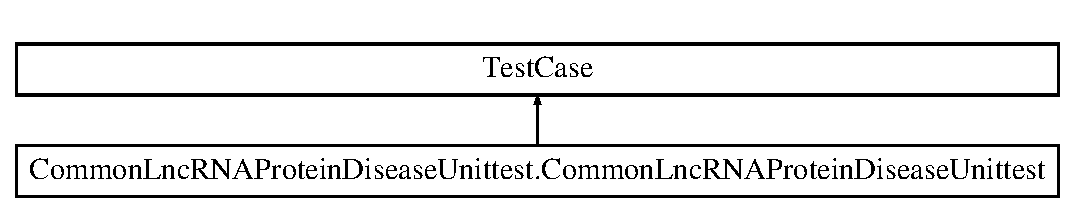
\includegraphics[height=2.000000cm]{classCommonLncRNAProteinDiseaseUnittest_1_1CommonLncRNAProteinDiseaseUnittest}
\end{center}
\end{figure}
\subsection*{Public Member Functions}
\begin{DoxyCompactItemize}
\item 
\hypertarget{classCommonLncRNAProteinDiseaseUnittest_1_1CommonLncRNAProteinDiseaseUnittest_a7bcfbf4031a279644d986e3a82ea6e9e}{def {\bfseries set\-Up}}\label{classCommonLncRNAProteinDiseaseUnittest_1_1CommonLncRNAProteinDiseaseUnittest_a7bcfbf4031a279644d986e3a82ea6e9e}

\item 
\hypertarget{classCommonLncRNAProteinDiseaseUnittest_1_1CommonLncRNAProteinDiseaseUnittest_a5e22d487d2400b87d71144e74e8efaf2}{def {\bfseries test\-\_\-enrichment\-\_\-to\-\_\-protein}}\label{classCommonLncRNAProteinDiseaseUnittest_1_1CommonLncRNAProteinDiseaseUnittest_a5e22d487d2400b87d71144e74e8efaf2}

\item 
\hypertarget{classCommonLncRNAProteinDiseaseUnittest_1_1CommonLncRNAProteinDiseaseUnittest_aeb4eee9484596b175e229e276071676a}{def {\bfseries test\-\_\-process\-\_\-lncrna\-\_\-protein\-\_\-map}}\label{classCommonLncRNAProteinDiseaseUnittest_1_1CommonLncRNAProteinDiseaseUnittest_aeb4eee9484596b175e229e276071676a}

\item 
\hypertarget{classCommonLncRNAProteinDiseaseUnittest_1_1CommonLncRNAProteinDiseaseUnittest_ad0517c1b8b7d3247ec958f6120ab842c}{def {\bfseries test\-\_\-read\-\_\-rainet\-\_\-db}}\label{classCommonLncRNAProteinDiseaseUnittest_1_1CommonLncRNAProteinDiseaseUnittest_ad0517c1b8b7d3247ec958f6120ab842c}

\item 
\hypertarget{classCommonLncRNAProteinDiseaseUnittest_1_1CommonLncRNAProteinDiseaseUnittest_a30b9ad221b3cffb58331f2daefadaaf2}{def {\bfseries test\-\_\-read\-\_\-lncrna\-\_\-disease\-\_\-file}}\label{classCommonLncRNAProteinDiseaseUnittest_1_1CommonLncRNAProteinDiseaseUnittest_a30b9ad221b3cffb58331f2daefadaaf2}

\item 
\hypertarget{classCommonLncRNAProteinDiseaseUnittest_1_1CommonLncRNAProteinDiseaseUnittest_ad49544999ca908706c1870bda5b9e000}{def {\bfseries test\-\_\-read\-\_\-protein\-\_\-disease\-\_\-file}}\label{classCommonLncRNAProteinDiseaseUnittest_1_1CommonLncRNAProteinDiseaseUnittest_ad49544999ca908706c1870bda5b9e000}

\item 
\hypertarget{classCommonLncRNAProteinDiseaseUnittest_1_1CommonLncRNAProteinDiseaseUnittest_a63e61c819750ca54d177a85af7724d09}{def {\bfseries test\-\_\-run}}\label{classCommonLncRNAProteinDiseaseUnittest_1_1CommonLncRNAProteinDiseaseUnittest_a63e61c819750ca54d177a85af7724d09}

\item 
\hypertarget{classCommonLncRNAProteinDiseaseUnittest_1_1CommonLncRNAProteinDiseaseUnittest_a9912b72e000611e962c8991b7d60591e}{def {\bfseries tear\-Down}}\label{classCommonLncRNAProteinDiseaseUnittest_1_1CommonLncRNAProteinDiseaseUnittest_a9912b72e000611e962c8991b7d60591e}

\end{DoxyCompactItemize}
\subsection*{Public Attributes}
\begin{DoxyCompactItemize}
\item 
\hypertarget{classCommonLncRNAProteinDiseaseUnittest_1_1CommonLncRNAProteinDiseaseUnittest_ab311405ca4aa65de104af7c79f33e369}{{\bfseries rainet\-D\-B}}\label{classCommonLncRNAProteinDiseaseUnittest_1_1CommonLncRNAProteinDiseaseUnittest_ab311405ca4aa65de104af7c79f33e369}

\item 
\hypertarget{classCommonLncRNAProteinDiseaseUnittest_1_1CommonLncRNAProteinDiseaseUnittest_a97daf04dfbbd0c551da46f6bc79710a3}{{\bfseries lnc\-R\-N\-A\-Disease\-File}}\label{classCommonLncRNAProteinDiseaseUnittest_1_1CommonLncRNAProteinDiseaseUnittest_a97daf04dfbbd0c551da46f6bc79710a3}

\item 
\hypertarget{classCommonLncRNAProteinDiseaseUnittest_1_1CommonLncRNAProteinDiseaseUnittest_ae0036fd0cab755a28c8e6d6d15eb5b5f}{{\bfseries protein\-Disease\-File}}\label{classCommonLncRNAProteinDiseaseUnittest_1_1CommonLncRNAProteinDiseaseUnittest_ae0036fd0cab755a28c8e6d6d15eb5b5f}

\item 
\hypertarget{classCommonLncRNAProteinDiseaseUnittest_1_1CommonLncRNAProteinDiseaseUnittest_aa512b0ff4def48577540b559d110f021}{{\bfseries enrichment\-Data}}\label{classCommonLncRNAProteinDiseaseUnittest_1_1CommonLncRNAProteinDiseaseUnittest_aa512b0ff4def48577540b559d110f021}

\item 
\hypertarget{classCommonLncRNAProteinDiseaseUnittest_1_1CommonLncRNAProteinDiseaseUnittest_a2b2461cac297e9b5bf8cf158a0f605b3}{{\bfseries output\-Folder}}\label{classCommonLncRNAProteinDiseaseUnittest_1_1CommonLncRNAProteinDiseaseUnittest_a2b2461cac297e9b5bf8cf158a0f605b3}

\item 
\hypertarget{classCommonLncRNAProteinDiseaseUnittest_1_1CommonLncRNAProteinDiseaseUnittest_aa9732ab65411523301c1de9a3cb528c7}{{\bfseries min\-Word\-Size}}\label{classCommonLncRNAProteinDiseaseUnittest_1_1CommonLncRNAProteinDiseaseUnittest_aa9732ab65411523301c1de9a3cb528c7}

\item 
\hypertarget{classCommonLncRNAProteinDiseaseUnittest_1_1CommonLncRNAProteinDiseaseUnittest_a5927af495df0bcea9888de16b7dffabc}{{\bfseries black\-Listed\-Words}}\label{classCommonLncRNAProteinDiseaseUnittest_1_1CommonLncRNAProteinDiseaseUnittest_a5927af495df0bcea9888de16b7dffabc}

\item 
\hypertarget{classCommonLncRNAProteinDiseaseUnittest_1_1CommonLncRNAProteinDiseaseUnittest_a6cdb4beaf2a54a29aba5656d55a41a27}{{\bfseries complex\-Datasets}}\label{classCommonLncRNAProteinDiseaseUnittest_1_1CommonLncRNAProteinDiseaseUnittest_a6cdb4beaf2a54a29aba5656d55a41a27}

\item 
\hypertarget{classCommonLncRNAProteinDiseaseUnittest_1_1CommonLncRNAProteinDiseaseUnittest_a654f59c6ee381e479d556a0b75ca71b0}{{\bfseries expected\-Folder}}\label{classCommonLncRNAProteinDiseaseUnittest_1_1CommonLncRNAProteinDiseaseUnittest_a654f59c6ee381e479d556a0b75ca71b0}

\item 
\hypertarget{classCommonLncRNAProteinDiseaseUnittest_1_1CommonLncRNAProteinDiseaseUnittest_a9bbdca0e6e0ecf24392db99078a4b53b}{{\bfseries run}}\label{classCommonLncRNAProteinDiseaseUnittest_1_1CommonLncRNAProteinDiseaseUnittest_a9bbdca0e6e0ecf24392db99078a4b53b}

\end{DoxyCompactItemize}


The documentation for this class was generated from the following file\-:\begin{DoxyCompactItemize}
\item 
test/fr/tagc/rainet/core/execution/analysis/\-Enrichment\-Analysis/Common\-Lnc\-R\-N\-A\-Protein\-Disease\-Unittest.\-py\end{DoxyCompactItemize}

\hypertarget{classsrc_1_1fr_1_1tagc_1_1rainet_1_1core_1_1execution_1_1analysis_1_1EnrichmentAnalysis_1_1Comple500f6ec22a9a1e615c8c425ff66b262}{\section{src.\-fr.\-tagc.\-rainet.\-core.\-execution.\-analysis.\-Enrichment\-Analysis.\-Complex\-Dataset\-Overlap.\-Complex\-Dataset\-Overlap Class Reference}
\label{classsrc_1_1fr_1_1tagc_1_1rainet_1_1core_1_1execution_1_1analysis_1_1EnrichmentAnalysis_1_1Comple500f6ec22a9a1e615c8c425ff66b262}\index{src.\-fr.\-tagc.\-rainet.\-core.\-execution.\-analysis.\-Enrichment\-Analysis.\-Complex\-Dataset\-Overlap.\-Complex\-Dataset\-Overlap@{src.\-fr.\-tagc.\-rainet.\-core.\-execution.\-analysis.\-Enrichment\-Analysis.\-Complex\-Dataset\-Overlap.\-Complex\-Dataset\-Overlap}}
}
Inheritance diagram for src.\-fr.\-tagc.\-rainet.\-core.\-execution.\-analysis.\-Enrichment\-Analysis.\-Complex\-Dataset\-Overlap.\-Complex\-Dataset\-Overlap\-:\begin{figure}[H]
\begin{center}
\leavevmode
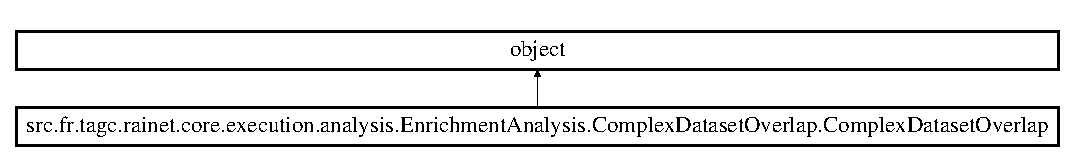
\includegraphics[height=1.728395cm]{classsrc_1_1fr_1_1tagc_1_1rainet_1_1core_1_1execution_1_1analysis_1_1EnrichmentAnalysis_1_1Comple500f6ec22a9a1e615c8c425ff66b262}
\end{center}
\end{figure}
\subsection*{Public Member Functions}
\begin{DoxyCompactItemize}
\item 
\hypertarget{classsrc_1_1fr_1_1tagc_1_1rainet_1_1core_1_1execution_1_1analysis_1_1EnrichmentAnalysis_1_1Comple500f6ec22a9a1e615c8c425ff66b262_a0bf4f8cb18243a81434b77cf039c7478}{def {\bfseries \-\_\-\-\_\-init\-\_\-\-\_\-}}\label{classsrc_1_1fr_1_1tagc_1_1rainet_1_1core_1_1execution_1_1analysis_1_1EnrichmentAnalysis_1_1Comple500f6ec22a9a1e615c8c425ff66b262_a0bf4f8cb18243a81434b77cf039c7478}

\item 
\hypertarget{classsrc_1_1fr_1_1tagc_1_1rainet_1_1core_1_1execution_1_1analysis_1_1EnrichmentAnalysis_1_1Comple500f6ec22a9a1e615c8c425ff66b262_ad199fae3088e9e1bb133f35d1f08a056}{def {\bfseries read\-\_\-rainet\-\_\-db}}\label{classsrc_1_1fr_1_1tagc_1_1rainet_1_1core_1_1execution_1_1analysis_1_1EnrichmentAnalysis_1_1Comple500f6ec22a9a1e615c8c425ff66b262_ad199fae3088e9e1bb133f35d1f08a056}

\item 
\hypertarget{classsrc_1_1fr_1_1tagc_1_1rainet_1_1core_1_1execution_1_1analysis_1_1EnrichmentAnalysis_1_1Comple500f6ec22a9a1e615c8c425ff66b262_ae2fdd47d271331fee66939779fc64e0c}{def {\bfseries intra\-\_\-dataset\-\_\-overlap}}\label{classsrc_1_1fr_1_1tagc_1_1rainet_1_1core_1_1execution_1_1analysis_1_1EnrichmentAnalysis_1_1Comple500f6ec22a9a1e615c8c425ff66b262_ae2fdd47d271331fee66939779fc64e0c}

\item 
\hypertarget{classsrc_1_1fr_1_1tagc_1_1rainet_1_1core_1_1execution_1_1analysis_1_1EnrichmentAnalysis_1_1Comple500f6ec22a9a1e615c8c425ff66b262_ab6353b4c5b1a75d78480193002c90a05}{def {\bfseries inter\-\_\-dataset\-\_\-overlap}}\label{classsrc_1_1fr_1_1tagc_1_1rainet_1_1core_1_1execution_1_1analysis_1_1EnrichmentAnalysis_1_1Comple500f6ec22a9a1e615c8c425ff66b262_ab6353b4c5b1a75d78480193002c90a05}

\end{DoxyCompactItemize}
\subsection*{Static Public Member Functions}
\begin{DoxyCompactItemize}
\item 
\hypertarget{classsrc_1_1fr_1_1tagc_1_1rainet_1_1core_1_1execution_1_1analysis_1_1EnrichmentAnalysis_1_1Comple500f6ec22a9a1e615c8c425ff66b262_a4788c69b13602999512a3c230d7694ad}{def {\bfseries group\-\_\-overlap}}\label{classsrc_1_1fr_1_1tagc_1_1rainet_1_1core_1_1execution_1_1analysis_1_1EnrichmentAnalysis_1_1Comple500f6ec22a9a1e615c8c425ff66b262_a4788c69b13602999512a3c230d7694ad}

\end{DoxyCompactItemize}
\subsection*{Public Attributes}
\begin{DoxyCompactItemize}
\item 
\hypertarget{classsrc_1_1fr_1_1tagc_1_1rainet_1_1core_1_1execution_1_1analysis_1_1EnrichmentAnalysis_1_1Comple500f6ec22a9a1e615c8c425ff66b262_aeec34421381653e1563ef6f4846a77dd}{{\bfseries rainet\-D\-B}}\label{classsrc_1_1fr_1_1tagc_1_1rainet_1_1core_1_1execution_1_1analysis_1_1EnrichmentAnalysis_1_1Comple500f6ec22a9a1e615c8c425ff66b262_aeec34421381653e1563ef6f4846a77dd}

\item 
\hypertarget{classsrc_1_1fr_1_1tagc_1_1rainet_1_1core_1_1execution_1_1analysis_1_1EnrichmentAnalysis_1_1Comple500f6ec22a9a1e615c8c425ff66b262_ae25f400f4184cb99fe709531cf2b6cd0}{{\bfseries output\-Folder}}\label{classsrc_1_1fr_1_1tagc_1_1rainet_1_1core_1_1execution_1_1analysis_1_1EnrichmentAnalysis_1_1Comple500f6ec22a9a1e615c8c425ff66b262_ae25f400f4184cb99fe709531cf2b6cd0}

\item 
\hypertarget{classsrc_1_1fr_1_1tagc_1_1rainet_1_1core_1_1execution_1_1analysis_1_1EnrichmentAnalysis_1_1Comple500f6ec22a9a1e615c8c425ff66b262_a3b52d1d2f44e69683f261b530d8f835e}{{\bfseries use\-Interacting\-Proteins}}\label{classsrc_1_1fr_1_1tagc_1_1rainet_1_1core_1_1execution_1_1analysis_1_1EnrichmentAnalysis_1_1Comple500f6ec22a9a1e615c8c425ff66b262_a3b52d1d2f44e69683f261b530d8f835e}

\item 
\hypertarget{classsrc_1_1fr_1_1tagc_1_1rainet_1_1core_1_1execution_1_1analysis_1_1EnrichmentAnalysis_1_1Comple500f6ec22a9a1e615c8c425ff66b262_a2510349280b69004bd9169ca1d32cc58}{{\bfseries high\-Overlap\-Stat}}\label{classsrc_1_1fr_1_1tagc_1_1rainet_1_1core_1_1execution_1_1analysis_1_1EnrichmentAnalysis_1_1Comple500f6ec22a9a1e615c8c425ff66b262_a2510349280b69004bd9169ca1d32cc58}

\item 
\hypertarget{classsrc_1_1fr_1_1tagc_1_1rainet_1_1core_1_1execution_1_1analysis_1_1EnrichmentAnalysis_1_1Comple500f6ec22a9a1e615c8c425ff66b262_a1377f3266bd5117dc335523896f4f385}{{\bfseries sql\-\_\-session}}\label{classsrc_1_1fr_1_1tagc_1_1rainet_1_1core_1_1execution_1_1analysis_1_1EnrichmentAnalysis_1_1Comple500f6ec22a9a1e615c8c425ff66b262_a1377f3266bd5117dc335523896f4f385}

\item 
\hypertarget{classsrc_1_1fr_1_1tagc_1_1rainet_1_1core_1_1execution_1_1analysis_1_1EnrichmentAnalysis_1_1Comple500f6ec22a9a1e615c8c425ff66b262_abae76ff4d3234fb0457b60c2d9cf9ab7}{{\bfseries list\-Datasets}}\label{classsrc_1_1fr_1_1tagc_1_1rainet_1_1core_1_1execution_1_1analysis_1_1EnrichmentAnalysis_1_1Comple500f6ec22a9a1e615c8c425ff66b262_abae76ff4d3234fb0457b60c2d9cf9ab7}

\item 
\hypertarget{classsrc_1_1fr_1_1tagc_1_1rainet_1_1core_1_1execution_1_1analysis_1_1EnrichmentAnalysis_1_1Comple500f6ec22a9a1e615c8c425ff66b262_a58a91eec8f3f4649f1be61334522250b}{{\bfseries interacting\-Proteins}}\label{classsrc_1_1fr_1_1tagc_1_1rainet_1_1core_1_1execution_1_1analysis_1_1EnrichmentAnalysis_1_1Comple500f6ec22a9a1e615c8c425ff66b262_a58a91eec8f3f4649f1be61334522250b}

\item 
\hypertarget{classsrc_1_1fr_1_1tagc_1_1rainet_1_1core_1_1execution_1_1analysis_1_1EnrichmentAnalysis_1_1Comple500f6ec22a9a1e615c8c425ff66b262_a8edd0a0a54f7905cb72ad2f3f42a9dbb}{{\bfseries dataset\-Dict}}\label{classsrc_1_1fr_1_1tagc_1_1rainet_1_1core_1_1execution_1_1analysis_1_1EnrichmentAnalysis_1_1Comple500f6ec22a9a1e615c8c425ff66b262_a8edd0a0a54f7905cb72ad2f3f42a9dbb}

\item 
\hypertarget{classsrc_1_1fr_1_1tagc_1_1rainet_1_1core_1_1execution_1_1analysis_1_1EnrichmentAnalysis_1_1Comple500f6ec22a9a1e615c8c425ff66b262_a7c41184d935425f4940e19d1cf0ad709}{{\bfseries intra\-Dataset\-Overlap}}\label{classsrc_1_1fr_1_1tagc_1_1rainet_1_1core_1_1execution_1_1analysis_1_1EnrichmentAnalysis_1_1Comple500f6ec22a9a1e615c8c425ff66b262_a7c41184d935425f4940e19d1cf0ad709}

\item 
\hypertarget{classsrc_1_1fr_1_1tagc_1_1rainet_1_1core_1_1execution_1_1analysis_1_1EnrichmentAnalysis_1_1Comple500f6ec22a9a1e615c8c425ff66b262_a86d0310015e03abafeb115476976ac53}{{\bfseries intra\-Dataset\-Overlap\-Results}}\label{classsrc_1_1fr_1_1tagc_1_1rainet_1_1core_1_1execution_1_1analysis_1_1EnrichmentAnalysis_1_1Comple500f6ec22a9a1e615c8c425ff66b262_a86d0310015e03abafeb115476976ac53}

\item 
\hypertarget{classsrc_1_1fr_1_1tagc_1_1rainet_1_1core_1_1execution_1_1analysis_1_1EnrichmentAnalysis_1_1Comple500f6ec22a9a1e615c8c425ff66b262_a01894db51aae17fc24c756cc3551ca6c}{{\bfseries inter\-Dataset\-Overlap}}\label{classsrc_1_1fr_1_1tagc_1_1rainet_1_1core_1_1execution_1_1analysis_1_1EnrichmentAnalysis_1_1Comple500f6ec22a9a1e615c8c425ff66b262_a01894db51aae17fc24c756cc3551ca6c}

\item 
\hypertarget{classsrc_1_1fr_1_1tagc_1_1rainet_1_1core_1_1execution_1_1analysis_1_1EnrichmentAnalysis_1_1Comple500f6ec22a9a1e615c8c425ff66b262_abd5782b7d735eab56d8f6a69b1cb6cc5}{{\bfseries inter\-Dataset\-Overlap\-Results}}\label{classsrc_1_1fr_1_1tagc_1_1rainet_1_1core_1_1execution_1_1analysis_1_1EnrichmentAnalysis_1_1Comple500f6ec22a9a1e615c8c425ff66b262_abd5782b7d735eab56d8f6a69b1cb6cc5}

\end{DoxyCompactItemize}
\subsection*{Static Public Attributes}
\begin{DoxyCompactItemize}
\item 
dictionary {\bfseries A\-N\-N\-O\-T\-A\-T\-I\-O\-N\-\_\-\-T\-A\-B\-L\-E\-S\-\_\-\-D\-I\-C\-T}
\item 
\hypertarget{classsrc_1_1fr_1_1tagc_1_1rainet_1_1core_1_1execution_1_1analysis_1_1EnrichmentAnalysis_1_1Comple500f6ec22a9a1e615c8c425ff66b262_aad332efb5616f17a939fa598621f0007}{string {\bfseries D\-E\-F\-A\-U\-L\-T\-\_\-\-D\-A\-T\-A\-S\-E\-T\-\_\-\-L\-I\-S\-T} = \char`\"{}Bioplex\-Cluster,Wan\-Cluster,Corum\-Cluster,Custom\-Cluster,Network\-Module\char`\"{}}\label{classsrc_1_1fr_1_1tagc_1_1rainet_1_1core_1_1execution_1_1analysis_1_1EnrichmentAnalysis_1_1Comple500f6ec22a9a1e615c8c425ff66b262_aad332efb5616f17a939fa598621f0007}

\item 
\hypertarget{classsrc_1_1fr_1_1tagc_1_1rainet_1_1core_1_1execution_1_1analysis_1_1EnrichmentAnalysis_1_1Comple500f6ec22a9a1e615c8c425ff66b262_a8d0c899ca889203c110ee554dc431ed8}{int {\bfseries D\-E\-F\-A\-U\-L\-T\-\_\-\-H\-I\-G\-H\-\_\-\-O\-V\-E\-R\-L\-A\-P} = 50}\label{classsrc_1_1fr_1_1tagc_1_1rainet_1_1core_1_1execution_1_1analysis_1_1EnrichmentAnalysis_1_1Comple500f6ec22a9a1e615c8c425ff66b262_a8d0c899ca889203c110ee554dc431ed8}

\item 
\hypertarget{classsrc_1_1fr_1_1tagc_1_1rainet_1_1core_1_1execution_1_1analysis_1_1EnrichmentAnalysis_1_1Comple500f6ec22a9a1e615c8c425ff66b262_a0cf4a867dc95e57acb1f8607591a7f5f}{string {\bfseries O\-U\-T\-P\-U\-T\-\_\-\-F\-I\-L\-E\-\_\-\-I\-N\-T\-R\-A\-\_\-\-D\-A\-T\-A\-S\-E\-T} = \char`\"{}intra\-\_\-dataset\-\_\-results.\-tsv\char`\"{}}\label{classsrc_1_1fr_1_1tagc_1_1rainet_1_1core_1_1execution_1_1analysis_1_1EnrichmentAnalysis_1_1Comple500f6ec22a9a1e615c8c425ff66b262_a0cf4a867dc95e57acb1f8607591a7f5f}

\item 
\hypertarget{classsrc_1_1fr_1_1tagc_1_1rainet_1_1core_1_1execution_1_1analysis_1_1EnrichmentAnalysis_1_1Comple500f6ec22a9a1e615c8c425ff66b262_a2f2745004b2b166e84a6c1de67de0b12}{string {\bfseries O\-U\-T\-P\-U\-T\-\_\-\-F\-I\-L\-E\-\_\-\-I\-N\-T\-E\-R\-\_\-\-D\-A\-T\-A\-S\-E\-T} = \char`\"{}inter\-\_\-dataset\-\_\-results.\-tsv\char`\"{}}\label{classsrc_1_1fr_1_1tagc_1_1rainet_1_1core_1_1execution_1_1analysis_1_1EnrichmentAnalysis_1_1Comple500f6ec22a9a1e615c8c425ff66b262_a2f2745004b2b166e84a6c1de67de0b12}

\end{DoxyCompactItemize}


\subsection{Member Data Documentation}
\hypertarget{classsrc_1_1fr_1_1tagc_1_1rainet_1_1core_1_1execution_1_1analysis_1_1EnrichmentAnalysis_1_1Comple500f6ec22a9a1e615c8c425ff66b262_a6339b1bc231875ff22b765265448638a}{\index{src\-::fr\-::tagc\-::rainet\-::core\-::execution\-::analysis\-::\-Enrichment\-Analysis\-::\-Complex\-Dataset\-Overlap\-::\-Complex\-Dataset\-Overlap@{src\-::fr\-::tagc\-::rainet\-::core\-::execution\-::analysis\-::\-Enrichment\-Analysis\-::\-Complex\-Dataset\-Overlap\-::\-Complex\-Dataset\-Overlap}!A\-N\-N\-O\-T\-A\-T\-I\-O\-N\-\_\-\-T\-A\-B\-L\-E\-S\-\_\-\-D\-I\-C\-T@{A\-N\-N\-O\-T\-A\-T\-I\-O\-N\-\_\-\-T\-A\-B\-L\-E\-S\-\_\-\-D\-I\-C\-T}}
\index{A\-N\-N\-O\-T\-A\-T\-I\-O\-N\-\_\-\-T\-A\-B\-L\-E\-S\-\_\-\-D\-I\-C\-T@{A\-N\-N\-O\-T\-A\-T\-I\-O\-N\-\_\-\-T\-A\-B\-L\-E\-S\-\_\-\-D\-I\-C\-T}!src::fr::tagc::rainet::core::execution::analysis::EnrichmentAnalysis::ComplexDatasetOverlap::ComplexDatasetOverlap@{src\-::fr\-::tagc\-::rainet\-::core\-::execution\-::analysis\-::\-Enrichment\-Analysis\-::\-Complex\-Dataset\-Overlap\-::\-Complex\-Dataset\-Overlap}}
\subsubsection[{A\-N\-N\-O\-T\-A\-T\-I\-O\-N\-\_\-\-T\-A\-B\-L\-E\-S\-\_\-\-D\-I\-C\-T}]{\setlength{\rightskip}{0pt plus 5cm}dictionary src.\-fr.\-tagc.\-rainet.\-core.\-execution.\-analysis.\-Enrichment\-Analysis.\-Complex\-Dataset\-Overlap.\-Complex\-Dataset\-Overlap.\-A\-N\-N\-O\-T\-A\-T\-I\-O\-N\-\_\-\-T\-A\-B\-L\-E\-S\-\_\-\-D\-I\-C\-T\hspace{0.3cm}{\ttfamily [static]}}}\label{classsrc_1_1fr_1_1tagc_1_1rainet_1_1core_1_1execution_1_1analysis_1_1EnrichmentAnalysis_1_1Comple500f6ec22a9a1e615c8c425ff66b262_a6339b1bc231875ff22b765265448638a}
{\bfseries Initial value\-:}
\begin{DoxyCode}
1 = \{\textcolor{stringliteral}{"NetworkModule"} : \textcolor{stringliteral}{"ProteinNetworkModule"},
2                               \textcolor{stringliteral}{"ReactomePathway"} : \textcolor{stringliteral}{"ProteinReactomeAnnotation"},
3                               \textcolor{stringliteral}{"KEGGPathway"} : \textcolor{stringliteral}{"ProteinKEGGAnnotation"},
4                               \textcolor{stringliteral}{"BioplexCluster"} : \textcolor{stringliteral}{"ProteinBioplexAnnotation"},
5                               \textcolor{stringliteral}{"WanCluster"} : \textcolor{stringliteral}{"ProteinWanAnnotation"},
6                               \textcolor{stringliteral}{"CorumCluster"} : \textcolor{stringliteral}{"ProteinCorumAnnotation"},
7                               \textcolor{stringliteral}{"CustomCluster"} : \textcolor{stringliteral}{"ProteinCustomAnnotation"}\}
\end{DoxyCode}


The documentation for this class was generated from the following file\-:\begin{DoxyCompactItemize}
\item 
src/fr/tagc/rainet/core/execution/analysis/\-Enrichment\-Analysis/Complex\-Dataset\-Overlap.\-py\end{DoxyCompactItemize}

\hypertarget{classComplexDatasetOverlapUnittest_1_1ComplexDatasetOverlapUnittest}{\section{Complex\-Dataset\-Overlap\-Unittest.\-Complex\-Dataset\-Overlap\-Unittest Class Reference}
\label{classComplexDatasetOverlapUnittest_1_1ComplexDatasetOverlapUnittest}\index{Complex\-Dataset\-Overlap\-Unittest.\-Complex\-Dataset\-Overlap\-Unittest@{Complex\-Dataset\-Overlap\-Unittest.\-Complex\-Dataset\-Overlap\-Unittest}}
}
Inheritance diagram for Complex\-Dataset\-Overlap\-Unittest.\-Complex\-Dataset\-Overlap\-Unittest\-:\begin{figure}[H]
\begin{center}
\leavevmode
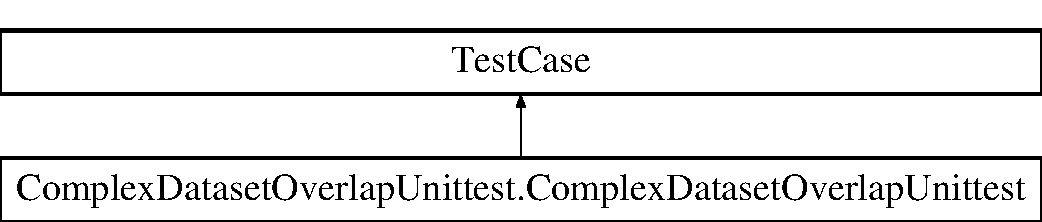
\includegraphics[height=2.000000cm]{classComplexDatasetOverlapUnittest_1_1ComplexDatasetOverlapUnittest}
\end{center}
\end{figure}
\subsection*{Public Member Functions}
\begin{DoxyCompactItemize}
\item 
\hypertarget{classComplexDatasetOverlapUnittest_1_1ComplexDatasetOverlapUnittest_aecdb2bcb8a179da12476106102c6c842}{def {\bfseries set\-Up}}\label{classComplexDatasetOverlapUnittest_1_1ComplexDatasetOverlapUnittest_aecdb2bcb8a179da12476106102c6c842}

\item 
\hypertarget{classComplexDatasetOverlapUnittest_1_1ComplexDatasetOverlapUnittest_a62388fe15f8f221992fce1ecab797f6f}{def {\bfseries test\-\_\-read\-\_\-rainet\-\_\-db}}\label{classComplexDatasetOverlapUnittest_1_1ComplexDatasetOverlapUnittest_a62388fe15f8f221992fce1ecab797f6f}

\item 
\hypertarget{classComplexDatasetOverlapUnittest_1_1ComplexDatasetOverlapUnittest_a48ba121b23e91db7d79b4821eee21a8c}{def {\bfseries test\-\_\-read\-\_\-rainet\-\_\-db\-\_\-two}}\label{classComplexDatasetOverlapUnittest_1_1ComplexDatasetOverlapUnittest_a48ba121b23e91db7d79b4821eee21a8c}

\item 
\hypertarget{classComplexDatasetOverlapUnittest_1_1ComplexDatasetOverlapUnittest_ab45fccb0e633e19d7d61a7d9a3c41e48}{def {\bfseries test\-\_\-group\-\_\-overlap}}\label{classComplexDatasetOverlapUnittest_1_1ComplexDatasetOverlapUnittest_ab45fccb0e633e19d7d61a7d9a3c41e48}

\item 
\hypertarget{classComplexDatasetOverlapUnittest_1_1ComplexDatasetOverlapUnittest_afdf421002101cfb4aefad67cc05d213b}{def {\bfseries test\-\_\-intra\-\_\-dataset\-\_\-overlap}}\label{classComplexDatasetOverlapUnittest_1_1ComplexDatasetOverlapUnittest_afdf421002101cfb4aefad67cc05d213b}

\item 
\hypertarget{classComplexDatasetOverlapUnittest_1_1ComplexDatasetOverlapUnittest_ae11f397b1b5124f14c270d80f892532e}{def {\bfseries test\-\_\-inter\-\_\-dataset\-\_\-overlap}}\label{classComplexDatasetOverlapUnittest_1_1ComplexDatasetOverlapUnittest_ae11f397b1b5124f14c270d80f892532e}

\end{DoxyCompactItemize}
\subsection*{Public Attributes}
\begin{DoxyCompactItemize}
\item 
\hypertarget{classComplexDatasetOverlapUnittest_1_1ComplexDatasetOverlapUnittest_ac97001e0c6b4e2c48b7edb2b696464fe}{{\bfseries rainet\-D\-B}}\label{classComplexDatasetOverlapUnittest_1_1ComplexDatasetOverlapUnittest_ac97001e0c6b4e2c48b7edb2b696464fe}

\item 
\hypertarget{classComplexDatasetOverlapUnittest_1_1ComplexDatasetOverlapUnittest_a9a3810558e594203613a63da0aab5988}{{\bfseries output\-Folder}}\label{classComplexDatasetOverlapUnittest_1_1ComplexDatasetOverlapUnittest_a9a3810558e594203613a63da0aab5988}

\item 
\hypertarget{classComplexDatasetOverlapUnittest_1_1ComplexDatasetOverlapUnittest_aaddfc23d86b63fe554070a78267e5e8c}{{\bfseries use\-Interacting\-Proteins}}\label{classComplexDatasetOverlapUnittest_1_1ComplexDatasetOverlapUnittest_aaddfc23d86b63fe554070a78267e5e8c}

\item 
\hypertarget{classComplexDatasetOverlapUnittest_1_1ComplexDatasetOverlapUnittest_a4db5ea8855111d8af8770f113c8f544c}{{\bfseries list\-Datasets}}\label{classComplexDatasetOverlapUnittest_1_1ComplexDatasetOverlapUnittest_a4db5ea8855111d8af8770f113c8f544c}

\item 
\hypertarget{classComplexDatasetOverlapUnittest_1_1ComplexDatasetOverlapUnittest_a0df45e97cbe1d1fa77bc87150637961b}{{\bfseries high\-Overlap\-Stat}}\label{classComplexDatasetOverlapUnittest_1_1ComplexDatasetOverlapUnittest_a0df45e97cbe1d1fa77bc87150637961b}

\item 
\hypertarget{classComplexDatasetOverlapUnittest_1_1ComplexDatasetOverlapUnittest_aafff157880bf8b16fe1c929f03693c12}{{\bfseries run}}\label{classComplexDatasetOverlapUnittest_1_1ComplexDatasetOverlapUnittest_aafff157880bf8b16fe1c929f03693c12}

\end{DoxyCompactItemize}


The documentation for this class was generated from the following file\-:\begin{DoxyCompactItemize}
\item 
test/fr/tagc/rainet/core/execution/analysis/\-Enrichment\-Analysis/Complex\-Dataset\-Overlap\-Unittest.\-py\end{DoxyCompactItemize}

\hypertarget{classsrc_1_1fr_1_1tagc_1_1rainet_1_1core_1_1data_1_1CorumCluster_1_1CorumCluster}{\section{src.\-fr.\-tagc.\-rainet.\-core.\-data.\-Corum\-Cluster.\-Corum\-Cluster Class Reference}
\label{classsrc_1_1fr_1_1tagc_1_1rainet_1_1core_1_1data_1_1CorumCluster_1_1CorumCluster}\index{src.\-fr.\-tagc.\-rainet.\-core.\-data.\-Corum\-Cluster.\-Corum\-Cluster@{src.\-fr.\-tagc.\-rainet.\-core.\-data.\-Corum\-Cluster.\-Corum\-Cluster}}
}
Inheritance diagram for src.\-fr.\-tagc.\-rainet.\-core.\-data.\-Corum\-Cluster.\-Corum\-Cluster\-:\begin{figure}[H]
\begin{center}
\leavevmode
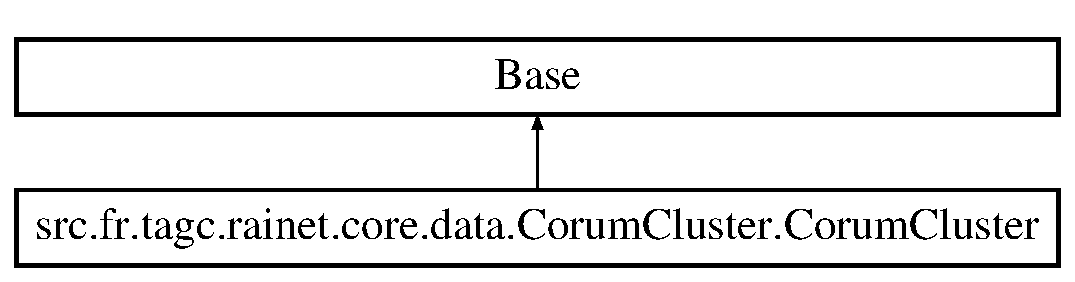
\includegraphics[height=2.000000cm]{classsrc_1_1fr_1_1tagc_1_1rainet_1_1core_1_1data_1_1CorumCluster_1_1CorumCluster}
\end{center}
\end{figure}
\subsection*{Public Member Functions}
\begin{DoxyCompactItemize}
\item 
\hypertarget{classsrc_1_1fr_1_1tagc_1_1rainet_1_1core_1_1data_1_1CorumCluster_1_1CorumCluster_ae945d7c9dbac5803b9cd9a5ba0888837}{def {\bfseries \-\_\-\-\_\-init\-\_\-\-\_\-}}\label{classsrc_1_1fr_1_1tagc_1_1rainet_1_1core_1_1data_1_1CorumCluster_1_1CorumCluster_ae945d7c9dbac5803b9cd9a5ba0888837}

\item 
\hypertarget{classsrc_1_1fr_1_1tagc_1_1rainet_1_1core_1_1data_1_1CorumCluster_1_1CorumCluster_a1e899e59d0ea4f49ed07fdbaf23d0ad7}{def \hyperlink{classsrc_1_1fr_1_1tagc_1_1rainet_1_1core_1_1data_1_1CorumCluster_1_1CorumCluster_a1e899e59d0ea4f49ed07fdbaf23d0ad7}{add\-\_\-to\-\_\-session}}\label{classsrc_1_1fr_1_1tagc_1_1rainet_1_1core_1_1data_1_1CorumCluster_1_1CorumCluster_a1e899e59d0ea4f49ed07fdbaf23d0ad7}

\begin{DoxyCompactList}\small\item\em Add the object to S\-Q\-L\-Alchemy session if it is linked to a protein. \end{DoxyCompactList}\item 
\hypertarget{classsrc_1_1fr_1_1tagc_1_1rainet_1_1core_1_1data_1_1CorumCluster_1_1CorumCluster_a0e8f530271c6ea21a5ef2b9f2b2c5d58}{def \hyperlink{classsrc_1_1fr_1_1tagc_1_1rainet_1_1core_1_1data_1_1CorumCluster_1_1CorumCluster_a0e8f530271c6ea21a5ef2b9f2b2c5d58}{add\-\_\-annotated\-\_\-protein}}\label{classsrc_1_1fr_1_1tagc_1_1rainet_1_1core_1_1data_1_1CorumCluster_1_1CorumCluster_a0e8f530271c6ea21a5ef2b9f2b2c5d58}

\begin{DoxyCompactList}\small\item\em Add an annotated protein to the list. \end{DoxyCompactList}\end{DoxyCompactItemize}
\subsection*{Public Attributes}
\begin{DoxyCompactItemize}
\item 
\hypertarget{classsrc_1_1fr_1_1tagc_1_1rainet_1_1core_1_1data_1_1CorumCluster_1_1CorumCluster_aac7961e0781cb05e9217461132c932e2}{{\bfseries cluster\-I\-D}}\label{classsrc_1_1fr_1_1tagc_1_1rainet_1_1core_1_1data_1_1CorumCluster_1_1CorumCluster_aac7961e0781cb05e9217461132c932e2}

\item 
\hypertarget{classsrc_1_1fr_1_1tagc_1_1rainet_1_1core_1_1data_1_1CorumCluster_1_1CorumCluster_a6d14e11bac6b1fe26765648cf863b049}{{\bfseries cluster\-Name}}\label{classsrc_1_1fr_1_1tagc_1_1rainet_1_1core_1_1data_1_1CorumCluster_1_1CorumCluster_a6d14e11bac6b1fe26765648cf863b049}

\item 
\hypertarget{classsrc_1_1fr_1_1tagc_1_1rainet_1_1core_1_1data_1_1CorumCluster_1_1CorumCluster_a31a4da28f7f583d75e11cd21a22ba407}{{\bfseries cluster\-Method}}\label{classsrc_1_1fr_1_1tagc_1_1rainet_1_1core_1_1data_1_1CorumCluster_1_1CorumCluster_a31a4da28f7f583d75e11cd21a22ba407}

\end{DoxyCompactItemize}
\subsection*{Static Public Attributes}
\begin{DoxyCompactItemize}
\item 
\hypertarget{classsrc_1_1fr_1_1tagc_1_1rainet_1_1core_1_1data_1_1CorumCluster_1_1CorumCluster_a9d78430da10cb503f5f89091222c6059}{tuple {\bfseries cluster\-I\-D} = Column( String, primary\-\_\-key = True )}\label{classsrc_1_1fr_1_1tagc_1_1rainet_1_1core_1_1data_1_1CorumCluster_1_1CorumCluster_a9d78430da10cb503f5f89091222c6059}

\item 
\hypertarget{classsrc_1_1fr_1_1tagc_1_1rainet_1_1core_1_1data_1_1CorumCluster_1_1CorumCluster_aaed5930ff71b9f3c9ccd19d0397d07b4}{tuple {\bfseries cluster\-Name} = Column( String)}\label{classsrc_1_1fr_1_1tagc_1_1rainet_1_1core_1_1data_1_1CorumCluster_1_1CorumCluster_aaed5930ff71b9f3c9ccd19d0397d07b4}

\item 
\hypertarget{classsrc_1_1fr_1_1tagc_1_1rainet_1_1core_1_1data_1_1CorumCluster_1_1CorumCluster_ae60fe6261540bfbf0b84c6d26db3510e}{tuple {\bfseries cluster\-Method} = Column( String)}\label{classsrc_1_1fr_1_1tagc_1_1rainet_1_1core_1_1data_1_1CorumCluster_1_1CorumCluster_ae60fe6261540bfbf0b84c6d26db3510e}

\item 
\hypertarget{classsrc_1_1fr_1_1tagc_1_1rainet_1_1core_1_1data_1_1CorumCluster_1_1CorumCluster_add238654f24b6cdcd703f1f391fcf544}{tuple {\bfseries annotated\-Proteins} = relationship('Protein', secondary=Protein\-Corum\-Annotation.\-\_\-\-\_\-table\-\_\-\-\_\-, backref=\char`\"{}Corum\-Annotations\char`\"{})}\label{classsrc_1_1fr_1_1tagc_1_1rainet_1_1core_1_1data_1_1CorumCluster_1_1CorumCluster_add238654f24b6cdcd703f1f391fcf544}

\end{DoxyCompactItemize}


The documentation for this class was generated from the following file\-:\begin{DoxyCompactItemize}
\item 
src/fr/tagc/rainet/core/data/Corum\-Cluster.\-py\end{DoxyCompactItemize}

\hypertarget{classsrc_1_1fr_1_1tagc_1_1rainet_1_1core_1_1data_1_1CustomCluster_1_1CustomCluster}{\section{src.\-fr.\-tagc.\-rainet.\-core.\-data.\-Custom\-Cluster.\-Custom\-Cluster Class Reference}
\label{classsrc_1_1fr_1_1tagc_1_1rainet_1_1core_1_1data_1_1CustomCluster_1_1CustomCluster}\index{src.\-fr.\-tagc.\-rainet.\-core.\-data.\-Custom\-Cluster.\-Custom\-Cluster@{src.\-fr.\-tagc.\-rainet.\-core.\-data.\-Custom\-Cluster.\-Custom\-Cluster}}
}
Inheritance diagram for src.\-fr.\-tagc.\-rainet.\-core.\-data.\-Custom\-Cluster.\-Custom\-Cluster\-:\begin{figure}[H]
\begin{center}
\leavevmode
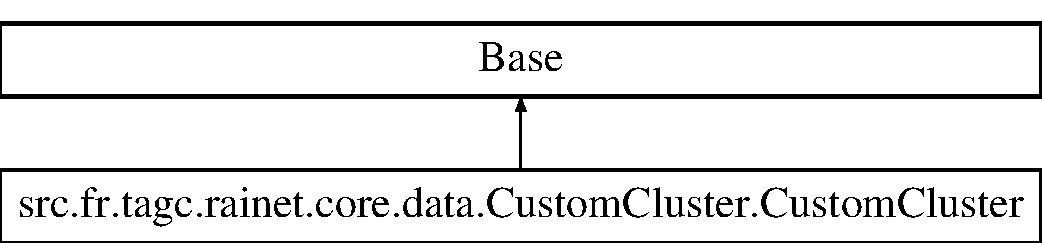
\includegraphics[height=2.000000cm]{classsrc_1_1fr_1_1tagc_1_1rainet_1_1core_1_1data_1_1CustomCluster_1_1CustomCluster}
\end{center}
\end{figure}
\subsection*{Public Member Functions}
\begin{DoxyCompactItemize}
\item 
\hypertarget{classsrc_1_1fr_1_1tagc_1_1rainet_1_1core_1_1data_1_1CustomCluster_1_1CustomCluster_adaa4bd6ef404a16b8deb4074bd214329}{def {\bfseries \-\_\-\-\_\-init\-\_\-\-\_\-}}\label{classsrc_1_1fr_1_1tagc_1_1rainet_1_1core_1_1data_1_1CustomCluster_1_1CustomCluster_adaa4bd6ef404a16b8deb4074bd214329}

\item 
\hypertarget{classsrc_1_1fr_1_1tagc_1_1rainet_1_1core_1_1data_1_1CustomCluster_1_1CustomCluster_a8b984de9fd4ea435c23a3016a6a34e48}{def \hyperlink{classsrc_1_1fr_1_1tagc_1_1rainet_1_1core_1_1data_1_1CustomCluster_1_1CustomCluster_a8b984de9fd4ea435c23a3016a6a34e48}{add\-\_\-to\-\_\-session}}\label{classsrc_1_1fr_1_1tagc_1_1rainet_1_1core_1_1data_1_1CustomCluster_1_1CustomCluster_a8b984de9fd4ea435c23a3016a6a34e48}

\begin{DoxyCompactList}\small\item\em Add the object to S\-Q\-L\-Alchemy session if it is linked to a protein. \end{DoxyCompactList}\item 
\hypertarget{classsrc_1_1fr_1_1tagc_1_1rainet_1_1core_1_1data_1_1CustomCluster_1_1CustomCluster_a81acb2f53b6edb6c78b3641f7f1b9fbf}{def \hyperlink{classsrc_1_1fr_1_1tagc_1_1rainet_1_1core_1_1data_1_1CustomCluster_1_1CustomCluster_a81acb2f53b6edb6c78b3641f7f1b9fbf}{add\-\_\-annotated\-\_\-protein}}\label{classsrc_1_1fr_1_1tagc_1_1rainet_1_1core_1_1data_1_1CustomCluster_1_1CustomCluster_a81acb2f53b6edb6c78b3641f7f1b9fbf}

\begin{DoxyCompactList}\small\item\em Add an annotated protein to the list. \end{DoxyCompactList}\end{DoxyCompactItemize}
\subsection*{Public Attributes}
\begin{DoxyCompactItemize}
\item 
\hypertarget{classsrc_1_1fr_1_1tagc_1_1rainet_1_1core_1_1data_1_1CustomCluster_1_1CustomCluster_a327be486227822b7d1a6ec95bfb98757}{{\bfseries cluster\-I\-D}}\label{classsrc_1_1fr_1_1tagc_1_1rainet_1_1core_1_1data_1_1CustomCluster_1_1CustomCluster_a327be486227822b7d1a6ec95bfb98757}

\end{DoxyCompactItemize}
\subsection*{Static Public Attributes}
\begin{DoxyCompactItemize}
\item 
\hypertarget{classsrc_1_1fr_1_1tagc_1_1rainet_1_1core_1_1data_1_1CustomCluster_1_1CustomCluster_ab59a52793c1e4b8080db2a0d2e094dd0}{tuple {\bfseries cluster\-I\-D} = Column( String, primary\-\_\-key = True )}\label{classsrc_1_1fr_1_1tagc_1_1rainet_1_1core_1_1data_1_1CustomCluster_1_1CustomCluster_ab59a52793c1e4b8080db2a0d2e094dd0}

\item 
\hypertarget{classsrc_1_1fr_1_1tagc_1_1rainet_1_1core_1_1data_1_1CustomCluster_1_1CustomCluster_add6b3e26c61496de9cadfa292346ce86}{tuple {\bfseries annotated\-Proteins} = relationship('Protein', secondary=Protein\-Custom\-Annotation.\-\_\-\-\_\-table\-\_\-\-\_\-, backref=\char`\"{}Custom\-Annotations\char`\"{})}\label{classsrc_1_1fr_1_1tagc_1_1rainet_1_1core_1_1data_1_1CustomCluster_1_1CustomCluster_add6b3e26c61496de9cadfa292346ce86}

\end{DoxyCompactItemize}


The documentation for this class was generated from the following file\-:\begin{DoxyCompactItemize}
\item 
src/fr/tagc/rainet/core/data/Custom\-Cluster.\-py\end{DoxyCompactItemize}

\hypertarget{classsrc_1_1fr_1_1tagc_1_1rainet_1_1core_1_1util_1_1factory_1_1DataFactory_1_1DataFactory}{\section{src.\-fr.\-tagc.\-rainet.\-core.\-util.\-factory.\-Data\-Factory.\-Data\-Factory Class Reference}
\label{classsrc_1_1fr_1_1tagc_1_1rainet_1_1core_1_1util_1_1factory_1_1DataFactory_1_1DataFactory}\index{src.\-fr.\-tagc.\-rainet.\-core.\-util.\-factory.\-Data\-Factory.\-Data\-Factory@{src.\-fr.\-tagc.\-rainet.\-core.\-util.\-factory.\-Data\-Factory.\-Data\-Factory}}
}


This class is a Factory that aims to create objects of various Class from class name and required parameters.  


\subsection*{Public Member Functions}
\begin{DoxyCompactItemize}
\item 
\hypertarget{classsrc_1_1fr_1_1tagc_1_1rainet_1_1core_1_1util_1_1factory_1_1DataFactory_1_1DataFactory_a7f7fc28351f88b2e831eb67cf63cb3a9}{def {\bfseries \-\_\-\-\_\-init\-\_\-\-\_\-}}\label{classsrc_1_1fr_1_1tagc_1_1rainet_1_1core_1_1util_1_1factory_1_1DataFactory_1_1DataFactory_a7f7fc28351f88b2e831eb67cf63cb3a9}

\item 
\hypertarget{classsrc_1_1fr_1_1tagc_1_1rainet_1_1core_1_1util_1_1factory_1_1DataFactory_1_1DataFactory_a1768d12461502c1a45de649c00bb6f61}{def \hyperlink{classsrc_1_1fr_1_1tagc_1_1rainet_1_1core_1_1util_1_1factory_1_1DataFactory_1_1DataFactory_a1768d12461502c1a45de649c00bb6f61}{clean\-\_\-table}}\label{classsrc_1_1fr_1_1tagc_1_1rainet_1_1core_1_1util_1_1factory_1_1DataFactory_1_1DataFactory_a1768d12461502c1a45de649c00bb6f61}

\begin{DoxyCompactList}\small\item\em Remove the content of the given table. \end{DoxyCompactList}\item 
def \hyperlink{classsrc_1_1fr_1_1tagc_1_1rainet_1_1core_1_1util_1_1factory_1_1DataFactory_1_1DataFactory_ab8f8da36aace01b8729585a7e4e5622a}{create\-\_\-object\-\_\-from\-\_\-tsv}
\begin{DoxyCompactList}\small\item\em Create an instance of the given class with the given parameters using the correct constructor Insert the instance to database using the S\-Q\-L session provided at Factory creation. \end{DoxyCompactList}\item 
\hypertarget{classsrc_1_1fr_1_1tagc_1_1rainet_1_1core_1_1util_1_1factory_1_1DataFactory_1_1DataFactory_a166db7f68a223633ef3a3caa38f1e25c}{def {\bfseries create\-\_\-object\-\_\-from\-\_\-fasta}}\label{classsrc_1_1fr_1_1tagc_1_1rainet_1_1core_1_1util_1_1factory_1_1DataFactory_1_1DataFactory_a166db7f68a223633ef3a3caa38f1e25c}

\end{DoxyCompactItemize}
\subsection*{Public Attributes}
\begin{DoxyCompactItemize}
\item 
\hypertarget{classsrc_1_1fr_1_1tagc_1_1rainet_1_1core_1_1util_1_1factory_1_1DataFactory_1_1DataFactory_a8d69a0748871157a2bba26ca797d4302}{{\bfseries class\-Name}}\label{classsrc_1_1fr_1_1tagc_1_1rainet_1_1core_1_1util_1_1factory_1_1DataFactory_1_1DataFactory_a8d69a0748871157a2bba26ca797d4302}

\end{DoxyCompactItemize}


\subsection{Detailed Description}
This class is a Factory that aims to create objects of various Class from class name and required parameters. 

The class manage the insertion to database of the newly created object and ensure its correct connection in the database schema. 

\subsection{Member Function Documentation}
\hypertarget{classsrc_1_1fr_1_1tagc_1_1rainet_1_1core_1_1util_1_1factory_1_1DataFactory_1_1DataFactory_ab8f8da36aace01b8729585a7e4e5622a}{\index{src\-::fr\-::tagc\-::rainet\-::core\-::util\-::factory\-::\-Data\-Factory\-::\-Data\-Factory@{src\-::fr\-::tagc\-::rainet\-::core\-::util\-::factory\-::\-Data\-Factory\-::\-Data\-Factory}!create\-\_\-object\-\_\-from\-\_\-tsv@{create\-\_\-object\-\_\-from\-\_\-tsv}}
\index{create\-\_\-object\-\_\-from\-\_\-tsv@{create\-\_\-object\-\_\-from\-\_\-tsv}!src::fr::tagc::rainet::core::util::factory::DataFactory::DataFactory@{src\-::fr\-::tagc\-::rainet\-::core\-::util\-::factory\-::\-Data\-Factory\-::\-Data\-Factory}}
\subsubsection[{create\-\_\-object\-\_\-from\-\_\-tsv}]{\setlength{\rightskip}{0pt plus 5cm}def src.\-fr.\-tagc.\-rainet.\-core.\-util.\-factory.\-Data\-Factory.\-Data\-Factory.\-create\-\_\-object\-\_\-from\-\_\-tsv (
\begin{DoxyParamCaption}
\item[{}]{self, }
\item[{}]{parameter\-\_\-value\-\_\-list}
\end{DoxyParamCaption}
)}}\label{classsrc_1_1fr_1_1tagc_1_1rainet_1_1core_1_1util_1_1factory_1_1DataFactory_1_1DataFactory_ab8f8da36aace01b8729585a7e4e5622a}


Create an instance of the given class with the given parameters using the correct constructor Insert the instance to database using the S\-Q\-L session provided at Factory creation. 


\begin{DoxyParams}{Parameters}
{\em class\-\_\-name} & \-: string -\/ the name of the Class to instantiate \\
\hline
{\em parameter\-\_\-value\-\_\-list} & \-: list -\/ the list of parameters values to be used to create the object\\
\hline
\end{DoxyParams}
Rainet\-Exception if an error occurred during object creation.

\begin{DoxyReturn}{Returns}
The created instance
\end{DoxyReturn}
Rainet\-Exception if an error occurred while building or inserting the new instance to the database 

The documentation for this class was generated from the following file\-:\begin{DoxyCompactItemize}
\item 
src/fr/tagc/rainet/core/util/factory/Data\-Factory.\-py\end{DoxyCompactItemize}

\hypertarget{classsrc_1_1fr_1_1tagc_1_1rainet_1_1core_1_1util_1_1data_1_1DataManager_1_1DataManager}{\section{src.\-fr.\-tagc.\-rainet.\-core.\-util.\-data.\-Data\-Manager.\-Data\-Manager Class Reference}
\label{classsrc_1_1fr_1_1tagc_1_1rainet_1_1core_1_1util_1_1data_1_1DataManager_1_1DataManager}\index{src.\-fr.\-tagc.\-rainet.\-core.\-util.\-data.\-Data\-Manager.\-Data\-Manager@{src.\-fr.\-tagc.\-rainet.\-core.\-util.\-data.\-Data\-Manager.\-Data\-Manager}}
}
Inheritance diagram for src.\-fr.\-tagc.\-rainet.\-core.\-util.\-data.\-Data\-Manager.\-Data\-Manager\-:\begin{figure}[H]
\begin{center}
\leavevmode
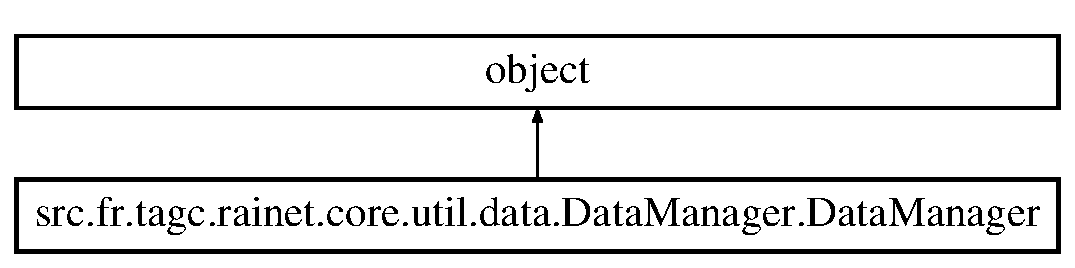
\includegraphics[height=2.000000cm]{classsrc_1_1fr_1_1tagc_1_1rainet_1_1core_1_1util_1_1data_1_1DataManager_1_1DataManager}
\end{center}
\end{figure}
\subsection*{Public Member Functions}
\begin{DoxyCompactItemize}
\item 
\hypertarget{classsrc_1_1fr_1_1tagc_1_1rainet_1_1core_1_1util_1_1data_1_1DataManager_1_1DataManager_a76a423800a2e6d1390fe73bb633e77d1}{def {\bfseries \-\_\-\-\_\-init\-\_\-\-\_\-}}\label{classsrc_1_1fr_1_1tagc_1_1rainet_1_1core_1_1util_1_1data_1_1DataManager_1_1DataManager_a76a423800a2e6d1390fe73bb633e77d1}

\item 
\hypertarget{classsrc_1_1fr_1_1tagc_1_1rainet_1_1core_1_1util_1_1data_1_1DataManager_1_1DataManager_a22822dafc9aae827dc6bcfc9fa6c02be}{def {\bfseries perform\-\_\-query}}\label{classsrc_1_1fr_1_1tagc_1_1rainet_1_1core_1_1util_1_1data_1_1DataManager_1_1DataManager_a22822dafc9aae827dc6bcfc9fa6c02be}

\item 
\hypertarget{classsrc_1_1fr_1_1tagc_1_1rainet_1_1core_1_1util_1_1data_1_1DataManager_1_1DataManager_aa281957d4633afb78c3b5210ad40ddd0}{def {\bfseries query\-\_\-to\-\_\-dict}}\label{classsrc_1_1fr_1_1tagc_1_1rainet_1_1core_1_1util_1_1data_1_1DataManager_1_1DataManager_aa281957d4633afb78c3b5210ad40ddd0}

\item 
\hypertarget{classsrc_1_1fr_1_1tagc_1_1rainet_1_1core_1_1util_1_1data_1_1DataManager_1_1DataManager_a7da97d73d8218fddfb6656d7556ab1d9}{def {\bfseries query\-\_\-to\-\_\-object\-\_\-dict}}\label{classsrc_1_1fr_1_1tagc_1_1rainet_1_1core_1_1util_1_1data_1_1DataManager_1_1DataManager_a7da97d73d8218fddfb6656d7556ab1d9}

\item 
\hypertarget{classsrc_1_1fr_1_1tagc_1_1rainet_1_1core_1_1util_1_1data_1_1DataManager_1_1DataManager_a10c906e202e0de8e88b98c9e12f18420}{def {\bfseries query\-\_\-to\-\_\-set}}\label{classsrc_1_1fr_1_1tagc_1_1rainet_1_1core_1_1util_1_1data_1_1DataManager_1_1DataManager_a10c906e202e0de8e88b98c9e12f18420}

\item 
\hypertarget{classsrc_1_1fr_1_1tagc_1_1rainet_1_1core_1_1util_1_1data_1_1DataManager_1_1DataManager_aa72d3137513a978d49d4bae3f04cd0c3}{def {\bfseries store\-\_\-data}}\label{classsrc_1_1fr_1_1tagc_1_1rainet_1_1core_1_1util_1_1data_1_1DataManager_1_1DataManager_aa72d3137513a978d49d4bae3f04cd0c3}

\item 
\hypertarget{classsrc_1_1fr_1_1tagc_1_1rainet_1_1core_1_1util_1_1data_1_1DataManager_1_1DataManager_aa1f82f1f0245b678dd6dbcba59f26eaa}{def {\bfseries get\-\_\-data}}\label{classsrc_1_1fr_1_1tagc_1_1rainet_1_1core_1_1util_1_1data_1_1DataManager_1_1DataManager_aa1f82f1f0245b678dd6dbcba59f26eaa}

\item 
\hypertarget{classsrc_1_1fr_1_1tagc_1_1rainet_1_1core_1_1util_1_1data_1_1DataManager_1_1DataManager_a5350a35b0602af140ab388e32a3f6f33}{def {\bfseries delete\-\_\-data}}\label{classsrc_1_1fr_1_1tagc_1_1rainet_1_1core_1_1util_1_1data_1_1DataManager_1_1DataManager_a5350a35b0602af140ab388e32a3f6f33}

\end{DoxyCompactItemize}
\subsection*{Static Public Member Functions}
\begin{DoxyCompactItemize}
\item 
\hypertarget{classsrc_1_1fr_1_1tagc_1_1rainet_1_1core_1_1util_1_1data_1_1DataManager_1_1DataManager_a750e63d4224d22065d333274a802bf22}{def {\bfseries get\-\_\-instance}}\label{classsrc_1_1fr_1_1tagc_1_1rainet_1_1core_1_1util_1_1data_1_1DataManager_1_1DataManager_a750e63d4224d22065d333274a802bf22}

\end{DoxyCompactItemize}
\subsection*{Public Attributes}
\begin{DoxyCompactItemize}
\item 
\hypertarget{classsrc_1_1fr_1_1tagc_1_1rainet_1_1core_1_1util_1_1data_1_1DataManager_1_1DataManager_a1869259f0c617d63a58ac8fbad135e55}{{\bfseries data}}\label{classsrc_1_1fr_1_1tagc_1_1rainet_1_1core_1_1util_1_1data_1_1DataManager_1_1DataManager_a1869259f0c617d63a58ac8fbad135e55}

\end{DoxyCompactItemize}


The documentation for this class was generated from the following file\-:\begin{DoxyCompactItemize}
\item 
src/fr/tagc/rainet/core/util/data/Data\-Manager.\-py\end{DoxyCompactItemize}

\hypertarget{classsrc_1_1fr_1_1tagc_1_1rainet_1_1core_1_1data_1_1DBParameter_1_1DBParameter}{\section{src.\-fr.\-tagc.\-rainet.\-core.\-data.\-D\-B\-Parameter.\-D\-B\-Parameter Class Reference}
\label{classsrc_1_1fr_1_1tagc_1_1rainet_1_1core_1_1data_1_1DBParameter_1_1DBParameter}\index{src.\-fr.\-tagc.\-rainet.\-core.\-data.\-D\-B\-Parameter.\-D\-B\-Parameter@{src.\-fr.\-tagc.\-rainet.\-core.\-data.\-D\-B\-Parameter.\-D\-B\-Parameter}}
}
Inheritance diagram for src.\-fr.\-tagc.\-rainet.\-core.\-data.\-D\-B\-Parameter.\-D\-B\-Parameter\-:\begin{figure}[H]
\begin{center}
\leavevmode
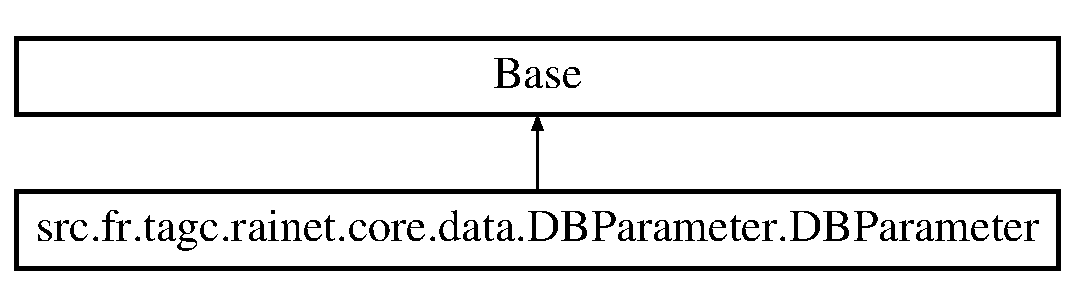
\includegraphics[height=2.000000cm]{classsrc_1_1fr_1_1tagc_1_1rainet_1_1core_1_1data_1_1DBParameter_1_1DBParameter}
\end{center}
\end{figure}
\subsection*{Public Member Functions}
\begin{DoxyCompactItemize}
\item 
\hypertarget{classsrc_1_1fr_1_1tagc_1_1rainet_1_1core_1_1data_1_1DBParameter_1_1DBParameter_ab8103a8f98dde9ad59b079e98e736f2b}{def {\bfseries \-\_\-\-\_\-init\-\_\-\-\_\-}}\label{classsrc_1_1fr_1_1tagc_1_1rainet_1_1core_1_1data_1_1DBParameter_1_1DBParameter_ab8103a8f98dde9ad59b079e98e736f2b}

\end{DoxyCompactItemize}
\subsection*{Public Attributes}
\begin{DoxyCompactItemize}
\item 
\hypertarget{classsrc_1_1fr_1_1tagc_1_1rainet_1_1core_1_1data_1_1DBParameter_1_1DBParameter_ae61b54e9c86bb19e10582ed189111596}{{\bfseries parameter\-Name}}\label{classsrc_1_1fr_1_1tagc_1_1rainet_1_1core_1_1data_1_1DBParameter_1_1DBParameter_ae61b54e9c86bb19e10582ed189111596}

\item 
\hypertarget{classsrc_1_1fr_1_1tagc_1_1rainet_1_1core_1_1data_1_1DBParameter_1_1DBParameter_a329f4dcded2890e7bab8ddb09e4fcec8}{{\bfseries parameter\-Type}}\label{classsrc_1_1fr_1_1tagc_1_1rainet_1_1core_1_1data_1_1DBParameter_1_1DBParameter_a329f4dcded2890e7bab8ddb09e4fcec8}

\item 
\hypertarget{classsrc_1_1fr_1_1tagc_1_1rainet_1_1core_1_1data_1_1DBParameter_1_1DBParameter_a7fcbbd77050aedcabcc665855c477015}{{\bfseries parameter\-Value}}\label{classsrc_1_1fr_1_1tagc_1_1rainet_1_1core_1_1data_1_1DBParameter_1_1DBParameter_a7fcbbd77050aedcabcc665855c477015}

\end{DoxyCompactItemize}
\subsection*{Static Public Attributes}
\begin{DoxyCompactItemize}
\item 
\hypertarget{classsrc_1_1fr_1_1tagc_1_1rainet_1_1core_1_1data_1_1DBParameter_1_1DBParameter_a86bcecbfa4d17d8ea0e7813d37099bfb}{tuple {\bfseries parameter\-Name} = Column( String, primary\-\_\-key = True )}\label{classsrc_1_1fr_1_1tagc_1_1rainet_1_1core_1_1data_1_1DBParameter_1_1DBParameter_a86bcecbfa4d17d8ea0e7813d37099bfb}

\item 
\hypertarget{classsrc_1_1fr_1_1tagc_1_1rainet_1_1core_1_1data_1_1DBParameter_1_1DBParameter_a11ca0d30425ea6e54214a55a7858306a}{tuple {\bfseries parameter\-Type} = Column( String )}\label{classsrc_1_1fr_1_1tagc_1_1rainet_1_1core_1_1data_1_1DBParameter_1_1DBParameter_a11ca0d30425ea6e54214a55a7858306a}

\item 
\hypertarget{classsrc_1_1fr_1_1tagc_1_1rainet_1_1core_1_1data_1_1DBParameter_1_1DBParameter_a9aa1907729ed16909500d246909e0649}{tuple {\bfseries parameter\-Value} = Column( String )}\label{classsrc_1_1fr_1_1tagc_1_1rainet_1_1core_1_1data_1_1DBParameter_1_1DBParameter_a9aa1907729ed16909500d246909e0649}

\end{DoxyCompactItemize}


The documentation for this class was generated from the following file\-:\begin{DoxyCompactItemize}
\item 
src/fr/tagc/rainet/core/data/D\-B\-Parameter.\-py\end{DoxyCompactItemize}

\hypertarget{classsrc_1_1fr_1_1tagc_1_1rainet_1_1core_1_1execution_1_1analysis_1_1EnrichmentAnalysis_1_1DiGeNfa669edf4ec9ad533f4e4738eca5d84d}{\section{src.\-fr.\-tagc.\-rainet.\-core.\-execution.\-analysis.\-Enrichment\-Analysis.\-Di\-Ge\-N\-E\-T\-Protein\-Disease.\-Di\-Ge\-N\-E\-T\-Protein\-Disease Class Reference}
\label{classsrc_1_1fr_1_1tagc_1_1rainet_1_1core_1_1execution_1_1analysis_1_1EnrichmentAnalysis_1_1DiGeNfa669edf4ec9ad533f4e4738eca5d84d}\index{src.\-fr.\-tagc.\-rainet.\-core.\-execution.\-analysis.\-Enrichment\-Analysis.\-Di\-Ge\-N\-E\-T\-Protein\-Disease.\-Di\-Ge\-N\-E\-T\-Protein\-Disease@{src.\-fr.\-tagc.\-rainet.\-core.\-execution.\-analysis.\-Enrichment\-Analysis.\-Di\-Ge\-N\-E\-T\-Protein\-Disease.\-Di\-Ge\-N\-E\-T\-Protein\-Disease}}
}
Inheritance diagram for src.\-fr.\-tagc.\-rainet.\-core.\-execution.\-analysis.\-Enrichment\-Analysis.\-Di\-Ge\-N\-E\-T\-Protein\-Disease.\-Di\-Ge\-N\-E\-T\-Protein\-Disease\-:\begin{figure}[H]
\begin{center}
\leavevmode
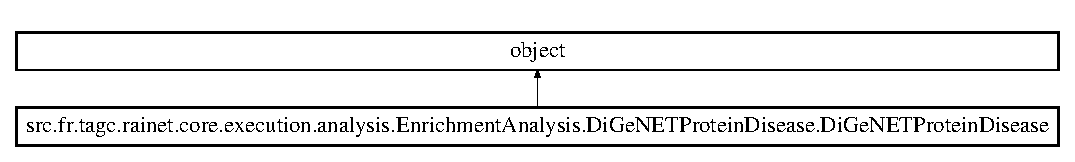
\includegraphics[height=1.723077cm]{classsrc_1_1fr_1_1tagc_1_1rainet_1_1core_1_1execution_1_1analysis_1_1EnrichmentAnalysis_1_1DiGeNfa669edf4ec9ad533f4e4738eca5d84d}
\end{center}
\end{figure}
\subsection*{Public Member Functions}
\begin{DoxyCompactItemize}
\item 
\hypertarget{classsrc_1_1fr_1_1tagc_1_1rainet_1_1core_1_1execution_1_1analysis_1_1EnrichmentAnalysis_1_1DiGeNfa669edf4ec9ad533f4e4738eca5d84d_a28b4a6c8b7fed53e80ec318380d44839}{def {\bfseries \-\_\-\-\_\-init\-\_\-\-\_\-}}\label{classsrc_1_1fr_1_1tagc_1_1rainet_1_1core_1_1execution_1_1analysis_1_1EnrichmentAnalysis_1_1DiGeNfa669edf4ec9ad533f4e4738eca5d84d_a28b4a6c8b7fed53e80ec318380d44839}

\item 
\hypertarget{classsrc_1_1fr_1_1tagc_1_1rainet_1_1core_1_1execution_1_1analysis_1_1EnrichmentAnalysis_1_1DiGeNfa669edf4ec9ad533f4e4738eca5d84d_a8976f94dfcca259ba66a55fe1685ac46}{def {\bfseries read\-\_\-digenet\-\_\-id\-\_\-mapping\-\_\-file}}\label{classsrc_1_1fr_1_1tagc_1_1rainet_1_1core_1_1execution_1_1analysis_1_1EnrichmentAnalysis_1_1DiGeNfa669edf4ec9ad533f4e4738eca5d84d_a8976f94dfcca259ba66a55fe1685ac46}

\item 
\hypertarget{classsrc_1_1fr_1_1tagc_1_1rainet_1_1core_1_1execution_1_1analysis_1_1EnrichmentAnalysis_1_1DiGeNfa669edf4ec9ad533f4e4738eca5d84d_a08be27a77bfebf3ae2b5e6a61f13bae3}{def {\bfseries read\-\_\-digenet\-\_\-file}}\label{classsrc_1_1fr_1_1tagc_1_1rainet_1_1core_1_1execution_1_1analysis_1_1EnrichmentAnalysis_1_1DiGeNfa669edf4ec9ad533f4e4738eca5d84d_a08be27a77bfebf3ae2b5e6a61f13bae3}

\end{DoxyCompactItemize}
\subsection*{Public Attributes}
\begin{DoxyCompactItemize}
\item 
\hypertarget{classsrc_1_1fr_1_1tagc_1_1rainet_1_1core_1_1execution_1_1analysis_1_1EnrichmentAnalysis_1_1DiGeNfa669edf4ec9ad533f4e4738eca5d84d_a154b5d8035088db13b0a8b51862496e9}{{\bfseries digenet\-I\-D\-Mapping\-File}}\label{classsrc_1_1fr_1_1tagc_1_1rainet_1_1core_1_1execution_1_1analysis_1_1EnrichmentAnalysis_1_1DiGeNfa669edf4ec9ad533f4e4738eca5d84d_a154b5d8035088db13b0a8b51862496e9}

\item 
\hypertarget{classsrc_1_1fr_1_1tagc_1_1rainet_1_1core_1_1execution_1_1analysis_1_1EnrichmentAnalysis_1_1DiGeNfa669edf4ec9ad533f4e4738eca5d84d_ac543a338fc51c78ddc9eb9f323ada8fa}{{\bfseries digenet\-File}}\label{classsrc_1_1fr_1_1tagc_1_1rainet_1_1core_1_1execution_1_1analysis_1_1EnrichmentAnalysis_1_1DiGeNfa669edf4ec9ad533f4e4738eca5d84d_ac543a338fc51c78ddc9eb9f323ada8fa}

\item 
\hypertarget{classsrc_1_1fr_1_1tagc_1_1rainet_1_1core_1_1execution_1_1analysis_1_1EnrichmentAnalysis_1_1DiGeNfa669edf4ec9ad533f4e4738eca5d84d_aebac14bf983c5ff6138e8ab356b0079a}{{\bfseries output\-Folder}}\label{classsrc_1_1fr_1_1tagc_1_1rainet_1_1core_1_1execution_1_1analysis_1_1EnrichmentAnalysis_1_1DiGeNfa669edf4ec9ad533f4e4738eca5d84d_aebac14bf983c5ff6138e8ab356b0079a}

\item 
\hypertarget{classsrc_1_1fr_1_1tagc_1_1rainet_1_1core_1_1execution_1_1analysis_1_1EnrichmentAnalysis_1_1DiGeNfa669edf4ec9ad533f4e4738eca5d84d_a427a6ca2e749da4e654b73e2f94d7b95}{{\bfseries min\-Digenet\-Score}}\label{classsrc_1_1fr_1_1tagc_1_1rainet_1_1core_1_1execution_1_1analysis_1_1EnrichmentAnalysis_1_1DiGeNfa669edf4ec9ad533f4e4738eca5d84d_a427a6ca2e749da4e654b73e2f94d7b95}

\item 
\hypertarget{classsrc_1_1fr_1_1tagc_1_1rainet_1_1core_1_1execution_1_1analysis_1_1EnrichmentAnalysis_1_1DiGeNfa669edf4ec9ad533f4e4738eca5d84d_a1501aaa44b3e74464cd7bf66f1a0777e}{{\bfseries digenet\-File\-Curated}}\label{classsrc_1_1fr_1_1tagc_1_1rainet_1_1core_1_1execution_1_1analysis_1_1EnrichmentAnalysis_1_1DiGeNfa669edf4ec9ad533f4e4738eca5d84d_a1501aaa44b3e74464cd7bf66f1a0777e}

\item 
\hypertarget{classsrc_1_1fr_1_1tagc_1_1rainet_1_1core_1_1execution_1_1analysis_1_1EnrichmentAnalysis_1_1DiGeNfa669edf4ec9ad533f4e4738eca5d84d_af37512a51a3acd315b7cc175b534a955}{{\bfseries out\-File}}\label{classsrc_1_1fr_1_1tagc_1_1rainet_1_1core_1_1execution_1_1analysis_1_1EnrichmentAnalysis_1_1DiGeNfa669edf4ec9ad533f4e4738eca5d84d_af37512a51a3acd315b7cc175b534a955}

\item 
\hypertarget{classsrc_1_1fr_1_1tagc_1_1rainet_1_1core_1_1execution_1_1analysis_1_1EnrichmentAnalysis_1_1DiGeNfa669edf4ec9ad533f4e4738eca5d84d_a6e7f0e694b0bbad7405d0ba5ccc02633}{{\bfseries entrez\-Uniprot\-Dict}}\label{classsrc_1_1fr_1_1tagc_1_1rainet_1_1core_1_1execution_1_1analysis_1_1EnrichmentAnalysis_1_1DiGeNfa669edf4ec9ad533f4e4738eca5d84d_a6e7f0e694b0bbad7405d0ba5ccc02633}

\end{DoxyCompactItemize}
\subsection*{Static Public Attributes}
\begin{DoxyCompactItemize}
\item 
\hypertarget{classsrc_1_1fr_1_1tagc_1_1rainet_1_1core_1_1execution_1_1analysis_1_1EnrichmentAnalysis_1_1DiGeNfa669edf4ec9ad533f4e4738eca5d84d_a3f8736ca9ac81864cbeaf54ee3100cf2}{string {\bfseries O\-U\-T\-P\-U\-T\-\_\-\-F\-I\-L\-E} = \char`\"{}/Di\-Ge\-N\-E\-T\-\_\-protein\-\_\-disease\-\_\-description\char`\"{}}\label{classsrc_1_1fr_1_1tagc_1_1rainet_1_1core_1_1execution_1_1analysis_1_1EnrichmentAnalysis_1_1DiGeNfa669edf4ec9ad533f4e4738eca5d84d_a3f8736ca9ac81864cbeaf54ee3100cf2}

\end{DoxyCompactItemize}


The documentation for this class was generated from the following file\-:\begin{DoxyCompactItemize}
\item 
src/fr/tagc/rainet/core/execution/analysis/\-Enrichment\-Analysis/Di\-Ge\-N\-E\-T\-Protein\-Disease.\-py\end{DoxyCompactItemize}

\hypertarget{classsrc_1_1core_1_1execution_1_1DisorderAnalysis_1_1DisorderAnalysis}{\section{src.\-core.\-execution.\-Disorder\-Analysis.\-Disorder\-Analysis Class Reference}
\label{classsrc_1_1core_1_1execution_1_1DisorderAnalysis_1_1DisorderAnalysis}\index{src.\-core.\-execution.\-Disorder\-Analysis.\-Disorder\-Analysis@{src.\-core.\-execution.\-Disorder\-Analysis.\-Disorder\-Analysis}}
}
\subsection*{Public Member Functions}
\begin{DoxyCompactItemize}
\item 
\hypertarget{classsrc_1_1core_1_1execution_1_1DisorderAnalysis_1_1DisorderAnalysis_a06547524f0853053afa867b43439b19a}{def {\bfseries change\-\_\-header}}\label{classsrc_1_1core_1_1execution_1_1DisorderAnalysis_1_1DisorderAnalysis_a06547524f0853053afa867b43439b19a}

\item 
\hypertarget{classsrc_1_1core_1_1execution_1_1DisorderAnalysis_1_1DisorderAnalysis_a922e091f1580ba686d0aa1f6ac62b34a}{def {\bfseries split\-\_\-dataset}}\label{classsrc_1_1core_1_1execution_1_1DisorderAnalysis_1_1DisorderAnalysis_a922e091f1580ba686d0aa1f6ac62b34a}

\item 
\hypertarget{classsrc_1_1core_1_1execution_1_1DisorderAnalysis_1_1DisorderAnalysis_a00e355ab6e99f45c43a07f91f9ad9360}{def {\bfseries anchor\-\_\-analysis}}\label{classsrc_1_1core_1_1execution_1_1DisorderAnalysis_1_1DisorderAnalysis_a00e355ab6e99f45c43a07f91f9ad9360}

\item 
\hypertarget{classsrc_1_1core_1_1execution_1_1DisorderAnalysis_1_1DisorderAnalysis_a1dfae98d95f41901c95faf52b797841e}{def {\bfseries iupred\-\_\-analysis}}\label{classsrc_1_1core_1_1execution_1_1DisorderAnalysis_1_1DisorderAnalysis_a1dfae98d95f41901c95faf52b797841e}

\item 
\hypertarget{classsrc_1_1core_1_1execution_1_1DisorderAnalysis_1_1DisorderAnalysis_a0456ea6250a3b9cb126dc04a385791df}{def {\bfseries analysis\-\_\-tools\-\_\-output}}\label{classsrc_1_1core_1_1execution_1_1DisorderAnalysis_1_1DisorderAnalysis_a0456ea6250a3b9cb126dc04a385791df}

\item 
\hypertarget{classsrc_1_1core_1_1execution_1_1DisorderAnalysis_1_1DisorderAnalysis_ad25eece82b9d869205cc4ca39f4fb930}{def {\bfseries disordpbind\-\_\-analysis}}\label{classsrc_1_1core_1_1execution_1_1DisorderAnalysis_1_1DisorderAnalysis_ad25eece82b9d869205cc4ca39f4fb930}

\item 
\hypertarget{classsrc_1_1core_1_1execution_1_1DisorderAnalysis_1_1DisorderAnalysis_a72fe1648d243781dd8ad73b204521fdc}{def {\bfseries particular\-\_\-analysis}}\label{classsrc_1_1core_1_1execution_1_1DisorderAnalysis_1_1DisorderAnalysis_a72fe1648d243781dd8ad73b204521fdc}

\end{DoxyCompactItemize}
\subsection*{Static Public Member Functions}
\begin{DoxyCompactItemize}
\item 
\hypertarget{classsrc_1_1core_1_1execution_1_1DisorderAnalysis_1_1DisorderAnalysis_a9f64ed2569e811d4c8db1549d8f0be9c}{def {\bfseries whole\-\_\-procedure}}\label{classsrc_1_1core_1_1execution_1_1DisorderAnalysis_1_1DisorderAnalysis_a9f64ed2569e811d4c8db1549d8f0be9c}

\end{DoxyCompactItemize}
\subsection*{Public Attributes}
\begin{DoxyCompactItemize}
\item 
\hypertarget{classsrc_1_1core_1_1execution_1_1DisorderAnalysis_1_1DisorderAnalysis_a1875381235a69a24436fa409f349a428}{{\bfseries path\-\_\-home}}\label{classsrc_1_1core_1_1execution_1_1DisorderAnalysis_1_1DisorderAnalysis_a1875381235a69a24436fa409f349a428}

\item 
\hypertarget{classsrc_1_1core_1_1execution_1_1DisorderAnalysis_1_1DisorderAnalysis_ac6b22ca9b11d0818132aba5e2cdf1147}{{\bfseries path\-\_\-input}}\label{classsrc_1_1core_1_1execution_1_1DisorderAnalysis_1_1DisorderAnalysis_ac6b22ca9b11d0818132aba5e2cdf1147}

\item 
\hypertarget{classsrc_1_1core_1_1execution_1_1DisorderAnalysis_1_1DisorderAnalysis_a392acd006ee59b96681c0836f6fb39eb}{{\bfseries namefile}}\label{classsrc_1_1core_1_1execution_1_1DisorderAnalysis_1_1DisorderAnalysis_a392acd006ee59b96681c0836f6fb39eb}

\item 
\hypertarget{classsrc_1_1core_1_1execution_1_1DisorderAnalysis_1_1DisorderAnalysis_a570df249633f3f0f1baca7cbc5058357}{{\bfseries path\-\_\-file\-\_\-input}}\label{classsrc_1_1core_1_1execution_1_1DisorderAnalysis_1_1DisorderAnalysis_a570df249633f3f0f1baca7cbc5058357}

\item 
\hypertarget{classsrc_1_1core_1_1execution_1_1DisorderAnalysis_1_1DisorderAnalysis_a4e1d12d39685d5296c774db62f811761}{{\bfseries path\-\_\-output}}\label{classsrc_1_1core_1_1execution_1_1DisorderAnalysis_1_1DisorderAnalysis_a4e1d12d39685d5296c774db62f811761}

\item 
\hypertarget{classsrc_1_1core_1_1execution_1_1DisorderAnalysis_1_1DisorderAnalysis_a41fd4e77d090eb427a63e6a4c863db02}{{\bfseries path\-\_\-file\-\_\-output}}\label{classsrc_1_1core_1_1execution_1_1DisorderAnalysis_1_1DisorderAnalysis_a41fd4e77d090eb427a63e6a4c863db02}

\item 
\hypertarget{classsrc_1_1core_1_1execution_1_1DisorderAnalysis_1_1DisorderAnalysis_a1836f4cd5491c3abdb077345ccc973dd}{{\bfseries source}}\label{classsrc_1_1core_1_1execution_1_1DisorderAnalysis_1_1DisorderAnalysis_a1836f4cd5491c3abdb077345ccc973dd}

\item 
\hypertarget{classsrc_1_1core_1_1execution_1_1DisorderAnalysis_1_1DisorderAnalysis_a799c202ea729368e7b1d28a608175f58}{{\bfseries type\-\_\-id}}\label{classsrc_1_1core_1_1execution_1_1DisorderAnalysis_1_1DisorderAnalysis_a799c202ea729368e7b1d28a608175f58}

\item 
\hypertarget{classsrc_1_1core_1_1execution_1_1DisorderAnalysis_1_1DisorderAnalysis_a535fd0ec64f536948175bea57e9066f5}{{\bfseries split\-\_\-path\-\_\-input}}\label{classsrc_1_1core_1_1execution_1_1DisorderAnalysis_1_1DisorderAnalysis_a535fd0ec64f536948175bea57e9066f5}

\item 
\hypertarget{classsrc_1_1core_1_1execution_1_1DisorderAnalysis_1_1DisorderAnalysis_a76b793198eeebe09d71e01a95c4ddbe6}{{\bfseries split\-\_\-file\-\_\-fasta}}\label{classsrc_1_1core_1_1execution_1_1DisorderAnalysis_1_1DisorderAnalysis_a76b793198eeebe09d71e01a95c4ddbe6}

\item 
\hypertarget{classsrc_1_1core_1_1execution_1_1DisorderAnalysis_1_1DisorderAnalysis_a7b8c229045873da55ed456e5f6e18ae5}{{\bfseries split\-\_\-path\-\_\-output}}\label{classsrc_1_1core_1_1execution_1_1DisorderAnalysis_1_1DisorderAnalysis_a7b8c229045873da55ed456e5f6e18ae5}

\item 
\hypertarget{classsrc_1_1core_1_1execution_1_1DisorderAnalysis_1_1DisorderAnalysis_afaacc164ca96f105e63938ab4ec16f56}{{\bfseries split\-\_\-start\-\_\-index}}\label{classsrc_1_1core_1_1execution_1_1DisorderAnalysis_1_1DisorderAnalysis_afaacc164ca96f105e63938ab4ec16f56}

\item 
\hypertarget{classsrc_1_1core_1_1execution_1_1DisorderAnalysis_1_1DisorderAnalysis_a0219eb110219fc7fec657a0d78e65175}{{\bfseries split\-\_\-end\-\_\-index}}\label{classsrc_1_1core_1_1execution_1_1DisorderAnalysis_1_1DisorderAnalysis_a0219eb110219fc7fec657a0d78e65175}

\item 
\hypertarget{classsrc_1_1core_1_1execution_1_1DisorderAnalysis_1_1DisorderAnalysis_a55f57eaf41274a78f1434f4762850f99}{{\bfseries tool\-\_\-path\-\_\-input}}\label{classsrc_1_1core_1_1execution_1_1DisorderAnalysis_1_1DisorderAnalysis_a55f57eaf41274a78f1434f4762850f99}

\item 
\hypertarget{classsrc_1_1core_1_1execution_1_1DisorderAnalysis_1_1DisorderAnalysis_afbe46d71e2276b054416ee296612731c}{{\bfseries anchor\-\_\-path\-\_\-output}}\label{classsrc_1_1core_1_1execution_1_1DisorderAnalysis_1_1DisorderAnalysis_afbe46d71e2276b054416ee296612731c}

\item 
\hypertarget{classsrc_1_1core_1_1execution_1_1DisorderAnalysis_1_1DisorderAnalysis_a7a01a4f2251bee5ea7bf5d119fa4de9d}{{\bfseries motif\-\_\-list\-\_\-path}}\label{classsrc_1_1core_1_1execution_1_1DisorderAnalysis_1_1DisorderAnalysis_a7a01a4f2251bee5ea7bf5d119fa4de9d}

\item 
\hypertarget{classsrc_1_1core_1_1execution_1_1DisorderAnalysis_1_1DisorderAnalysis_ad6211473f5599150bfdd6f1c604d7831}{{\bfseries iupred\-\_\-path\-\_\-output}}\label{classsrc_1_1core_1_1execution_1_1DisorderAnalysis_1_1DisorderAnalysis_ad6211473f5599150bfdd6f1c604d7831}

\item 
\hypertarget{classsrc_1_1core_1_1execution_1_1DisorderAnalysis_1_1DisorderAnalysis_a6870771b6eff47bc205c0d168349f57a}{{\bfseries input\-\_\-path\-\_\-iupred}}\label{classsrc_1_1core_1_1execution_1_1DisorderAnalysis_1_1DisorderAnalysis_a6870771b6eff47bc205c0d168349f57a}

\item 
\hypertarget{classsrc_1_1core_1_1execution_1_1DisorderAnalysis_1_1DisorderAnalysis_a96d8bf087f2fcbf9911d747c8ee52747}{{\bfseries output\-\_\-path\-\_\-analysis}}\label{classsrc_1_1core_1_1execution_1_1DisorderAnalysis_1_1DisorderAnalysis_a96d8bf087f2fcbf9911d747c8ee52747}

\item 
\hypertarget{classsrc_1_1core_1_1execution_1_1DisorderAnalysis_1_1DisorderAnalysis_a8b7d8b5e5f370b73f4d29db49fe97312}{{\bfseries threshold\-\_\-1}}\label{classsrc_1_1core_1_1execution_1_1DisorderAnalysis_1_1DisorderAnalysis_a8b7d8b5e5f370b73f4d29db49fe97312}

\item 
\hypertarget{classsrc_1_1core_1_1execution_1_1DisorderAnalysis_1_1DisorderAnalysis_a2c75eb7d9a59d1c5ae82b9500bf194af}{{\bfseries threshold\-\_\-2}}\label{classsrc_1_1core_1_1execution_1_1DisorderAnalysis_1_1DisorderAnalysis_a2c75eb7d9a59d1c5ae82b9500bf194af}

\item 
\hypertarget{classsrc_1_1core_1_1execution_1_1DisorderAnalysis_1_1DisorderAnalysis_a7ea3b7a9cdf780aa0e994b5595db2b3c}{{\bfseries number\-\_\-aa\-\_\-iupred}}\label{classsrc_1_1core_1_1execution_1_1DisorderAnalysis_1_1DisorderAnalysis_a7ea3b7a9cdf780aa0e994b5595db2b3c}

\item 
\hypertarget{classsrc_1_1core_1_1execution_1_1DisorderAnalysis_1_1DisorderAnalysis_a43bcb2025c02c8fd3e8819e0afea7274}{{\bfseries dataset\-\_\-type}}\label{classsrc_1_1core_1_1execution_1_1DisorderAnalysis_1_1DisorderAnalysis_a43bcb2025c02c8fd3e8819e0afea7274}

\item 
\hypertarget{classsrc_1_1core_1_1execution_1_1DisorderAnalysis_1_1DisorderAnalysis_a0ca4d8968869cef41a6f6ba6367870be}{{\bfseries input\-\_\-path\-\_\-anchor}}\label{classsrc_1_1core_1_1execution_1_1DisorderAnalysis_1_1DisorderAnalysis_a0ca4d8968869cef41a6f6ba6367870be}

\item 
\hypertarget{classsrc_1_1core_1_1execution_1_1DisorderAnalysis_1_1DisorderAnalysis_adac6fc979d1d27aca886e145cc9e44ee}{{\bfseries num\-\_\-aa\-\_\-anchor}}\label{classsrc_1_1core_1_1execution_1_1DisorderAnalysis_1_1DisorderAnalysis_adac6fc979d1d27aca886e145cc9e44ee}

\item 
\hypertarget{classsrc_1_1core_1_1execution_1_1DisorderAnalysis_1_1DisorderAnalysis_a2d78f2cb01940131fa70ce9edb020562}{{\bfseries input\-\_\-file}}\label{classsrc_1_1core_1_1execution_1_1DisorderAnalysis_1_1DisorderAnalysis_a2d78f2cb01940131fa70ce9edb020562}

\item 
\hypertarget{classsrc_1_1core_1_1execution_1_1DisorderAnalysis_1_1DisorderAnalysis_a8b452db0533c26c0c8da31f84da99518}{{\bfseries ouput\-\_\-path}}\label{classsrc_1_1core_1_1execution_1_1DisorderAnalysis_1_1DisorderAnalysis_a8b452db0533c26c0c8da31f84da99518}

\item 
\hypertarget{classsrc_1_1core_1_1execution_1_1DisorderAnalysis_1_1DisorderAnalysis_a20107bc715e646494b2409509af5efcf}{{\bfseries binding\-\_\-partner}}\label{classsrc_1_1core_1_1execution_1_1DisorderAnalysis_1_1DisorderAnalysis_a20107bc715e646494b2409509af5efcf}

\item 
\hypertarget{classsrc_1_1core_1_1execution_1_1DisorderAnalysis_1_1DisorderAnalysis_a21b2478fd2810a88e3c062d2513c2eb1}{{\bfseries num\-\_\-aa\-\_\-diso}}\label{classsrc_1_1core_1_1execution_1_1DisorderAnalysis_1_1DisorderAnalysis_a21b2478fd2810a88e3c062d2513c2eb1}

\item 
\hypertarget{classsrc_1_1core_1_1execution_1_1DisorderAnalysis_1_1DisorderAnalysis_af46c04812df3aab1f522489dfc51be04}{{\bfseries path\-\_\-input\-\_\-anchor\-\_\-file}}\label{classsrc_1_1core_1_1execution_1_1DisorderAnalysis_1_1DisorderAnalysis_af46c04812df3aab1f522489dfc51be04}

\item 
\hypertarget{classsrc_1_1core_1_1execution_1_1DisorderAnalysis_1_1DisorderAnalysis_ab883fe44f5882988198ab31e18b51b73}{{\bfseries path\-\_\-input\-\_\-iupred\-\_\-file}}\label{classsrc_1_1core_1_1execution_1_1DisorderAnalysis_1_1DisorderAnalysis_ab883fe44f5882988198ab31e18b51b73}

\item 
\hypertarget{classsrc_1_1core_1_1execution_1_1DisorderAnalysis_1_1DisorderAnalysis_afc33f47b7804dafa87593936c5bbb4aa}{{\bfseries path\-\_\-input\-\_\-disordp\-\_\-file}}\label{classsrc_1_1core_1_1execution_1_1DisorderAnalysis_1_1DisorderAnalysis_afc33f47b7804dafa87593936c5bbb4aa}

\item 
\hypertarget{classsrc_1_1core_1_1execution_1_1DisorderAnalysis_1_1DisorderAnalysis_abf94fe6afbceb17557826c3c11038817}{{\bfseries path\-\_\-input\-\_\-reg\-\_\-anchor}}\label{classsrc_1_1core_1_1execution_1_1DisorderAnalysis_1_1DisorderAnalysis_abf94fe6afbceb17557826c3c11038817}

\item 
\hypertarget{classsrc_1_1core_1_1execution_1_1DisorderAnalysis_1_1DisorderAnalysis_aebe8285284f1af93c8db075c4fac2d37}{{\bfseries path\-\_\-input\-\_\-reg\-\_\-iupred\-\_\-1}}\label{classsrc_1_1core_1_1execution_1_1DisorderAnalysis_1_1DisorderAnalysis_aebe8285284f1af93c8db075c4fac2d37}

\item 
\hypertarget{classsrc_1_1core_1_1execution_1_1DisorderAnalysis_1_1DisorderAnalysis_afa36b01b0efaf9be17f3c589b1adba81}{{\bfseries path\-\_\-input\-\_\-reg\-\_\-iupred\-\_\-2}}\label{classsrc_1_1core_1_1execution_1_1DisorderAnalysis_1_1DisorderAnalysis_afa36b01b0efaf9be17f3c589b1adba81}

\item 
\hypertarget{classsrc_1_1core_1_1execution_1_1DisorderAnalysis_1_1DisorderAnalysis_adb85cff23832d18eede844356bff3c88}{{\bfseries path\-\_\-input\-\_\-reg\-\_\-diso}}\label{classsrc_1_1core_1_1execution_1_1DisorderAnalysis_1_1DisorderAnalysis_adb85cff23832d18eede844356bff3c88}

\item 
\hypertarget{classsrc_1_1core_1_1execution_1_1DisorderAnalysis_1_1DisorderAnalysis_a6cc2aaacf00995e1c40cd950ba3dd988}{{\bfseries input\-\_\-files}}\label{classsrc_1_1core_1_1execution_1_1DisorderAnalysis_1_1DisorderAnalysis_a6cc2aaacf00995e1c40cd950ba3dd988}

\item 
\hypertarget{classsrc_1_1core_1_1execution_1_1DisorderAnalysis_1_1DisorderAnalysis_ab929d23afd4399deca3fbc40f27fc747}{{\bfseries list\-\_\-namefiles}}\label{classsrc_1_1core_1_1execution_1_1DisorderAnalysis_1_1DisorderAnalysis_ab929d23afd4399deca3fbc40f27fc747}

\item 
\hypertarget{classsrc_1_1core_1_1execution_1_1DisorderAnalysis_1_1DisorderAnalysis_a885957bccc650066ea7d33702ec860a4}{{\bfseries path\-\_\-output\-\_\-dir}}\label{classsrc_1_1core_1_1execution_1_1DisorderAnalysis_1_1DisorderAnalysis_a885957bccc650066ea7d33702ec860a4}

\item 
\hypertarget{classsrc_1_1core_1_1execution_1_1DisorderAnalysis_1_1DisorderAnalysis_af863d36c52828d6a11e5f0bb4168a6a8}{{\bfseries path\-\_\-output\-\_\-dir\-\_\-diso}}\label{classsrc_1_1core_1_1execution_1_1DisorderAnalysis_1_1DisorderAnalysis_af863d36c52828d6a11e5f0bb4168a6a8}

\item 
\hypertarget{classsrc_1_1core_1_1execution_1_1DisorderAnalysis_1_1DisorderAnalysis_a626e998d703fa66ea38897a98e06ca32}{{\bfseries protein\-\_\-column\-\_\-class}}\label{classsrc_1_1core_1_1execution_1_1DisorderAnalysis_1_1DisorderAnalysis_a626e998d703fa66ea38897a98e06ca32}

\end{DoxyCompactItemize}


The documentation for this class was generated from the following file\-:\begin{DoxyCompactItemize}
\item 
rbp-\/motif/src/core/execution/Disorder\-Analysis.\-py\end{DoxyCompactItemize}

\hypertarget{classsrc_1_1core_1_1util_1_1tools_1_1DisoRDPbind_1_1DisoRDPbind}{\section{src.\-core.\-util.\-tools.\-Diso\-R\-D\-Pbind.\-Diso\-R\-D\-Pbind Class Reference}
\label{classsrc_1_1core_1_1util_1_1tools_1_1DisoRDPbind_1_1DisoRDPbind}\index{src.\-core.\-util.\-tools.\-Diso\-R\-D\-Pbind.\-Diso\-R\-D\-Pbind@{src.\-core.\-util.\-tools.\-Diso\-R\-D\-Pbind.\-Diso\-R\-D\-Pbind}}
}
\subsection*{Static Public Member Functions}
\begin{DoxyCompactItemize}
\item 
\hypertarget{classsrc_1_1core_1_1util_1_1tools_1_1DisoRDPbind_1_1DisoRDPbind_a67d038b2f2d9d597cacc5e65c1d6f4e6}{def {\bfseries output\-\_\-reading}}\label{classsrc_1_1core_1_1util_1_1tools_1_1DisoRDPbind_1_1DisoRDPbind_a67d038b2f2d9d597cacc5e65c1d6f4e6}

\item 
\hypertarget{classsrc_1_1core_1_1util_1_1tools_1_1DisoRDPbind_1_1DisoRDPbind_ab3e4c7a45927bf1ad55081ed39853649}{def {\bfseries fraction\-\_\-calculation}}\label{classsrc_1_1core_1_1util_1_1tools_1_1DisoRDPbind_1_1DisoRDPbind_ab3e4c7a45927bf1ad55081ed39853649}

\item 
\hypertarget{classsrc_1_1core_1_1util_1_1tools_1_1DisoRDPbind_1_1DisoRDPbind_ad4a93b27f41380e426a360536393ffa9}{def {\bfseries disordp\-\_\-string\-\_\-info}}\label{classsrc_1_1core_1_1util_1_1tools_1_1DisoRDPbind_1_1DisoRDPbind_ad4a93b27f41380e426a360536393ffa9}

\item 
\hypertarget{classsrc_1_1core_1_1util_1_1tools_1_1DisoRDPbind_1_1DisoRDPbind_aff8e137007a6f1d68452870fa135eb31}{def {\bfseries make\-\_\-disordp\-\_\-file}}\label{classsrc_1_1core_1_1util_1_1tools_1_1DisoRDPbind_1_1DisoRDPbind_aff8e137007a6f1d68452870fa135eb31}

\end{DoxyCompactItemize}


The documentation for this class was generated from the following file\-:\begin{DoxyCompactItemize}
\item 
rbp-\/motif/src/core/util/tools/Diso\-R\-D\-Pbind.\-py\end{DoxyCompactItemize}

\hypertarget{classsrc_1_1core_1_1execution_1_1DownloadEnsemblSeq_1_1DownloadEnsemblSeq}{\section{src.\-core.\-execution.\-Download\-Ensembl\-Seq.\-Download\-Ensembl\-Seq Class Reference}
\label{classsrc_1_1core_1_1execution_1_1DownloadEnsemblSeq_1_1DownloadEnsemblSeq}\index{src.\-core.\-execution.\-Download\-Ensembl\-Seq.\-Download\-Ensembl\-Seq@{src.\-core.\-execution.\-Download\-Ensembl\-Seq.\-Download\-Ensembl\-Seq}}
}
\subsection*{Public Member Functions}
\begin{DoxyCompactItemize}
\item 
\hypertarget{classsrc_1_1core_1_1execution_1_1DownloadEnsemblSeq_1_1DownloadEnsemblSeq_a1874fd8859a6fc500d8511d27509124c}{def {\bfseries download\-\_\-product\-\_\-gene\-\_\-seq}}\label{classsrc_1_1core_1_1execution_1_1DownloadEnsemblSeq_1_1DownloadEnsemblSeq_a1874fd8859a6fc500d8511d27509124c}

\item 
\hypertarget{classsrc_1_1core_1_1execution_1_1DownloadEnsemblSeq_1_1DownloadEnsemblSeq_af36a9c6e46959bdaf0a98ab2c021825c}{def {\bfseries make\-\_\-dictionary}}\label{classsrc_1_1core_1_1execution_1_1DownloadEnsemblSeq_1_1DownloadEnsemblSeq_af36a9c6e46959bdaf0a98ab2c021825c}

\item 
\hypertarget{classsrc_1_1core_1_1execution_1_1DownloadEnsemblSeq_1_1DownloadEnsemblSeq_a20dc7983a7ea0e7c2cd49f6600ce9a09}{def {\bfseries get\-\_\-longest\-\_\-seq}}\label{classsrc_1_1core_1_1execution_1_1DownloadEnsemblSeq_1_1DownloadEnsemblSeq_a20dc7983a7ea0e7c2cd49f6600ce9a09}

\item 
\hypertarget{classsrc_1_1core_1_1execution_1_1DownloadEnsemblSeq_1_1DownloadEnsemblSeq_ad574c6879c68d335e8157f19300967ff}{def {\bfseries isoform\-\_\-sequences}}\label{classsrc_1_1core_1_1execution_1_1DownloadEnsemblSeq_1_1DownloadEnsemblSeq_ad574c6879c68d335e8157f19300967ff}

\item 
\hypertarget{classsrc_1_1core_1_1execution_1_1DownloadEnsemblSeq_1_1DownloadEnsemblSeq_ad430eda7b94bc924025db0727f46f460}{def {\bfseries merger\-\_\-sequences}}\label{classsrc_1_1core_1_1execution_1_1DownloadEnsemblSeq_1_1DownloadEnsemblSeq_ad430eda7b94bc924025db0727f46f460}

\end{DoxyCompactItemize}
\subsection*{Static Public Member Functions}
\begin{DoxyCompactItemize}
\item 
\hypertarget{classsrc_1_1core_1_1execution_1_1DownloadEnsemblSeq_1_1DownloadEnsemblSeq_aa94be4155b154d0ce7792e5ab9c25cc4}{def {\bfseries whole\-\_\-procedure}}\label{classsrc_1_1core_1_1execution_1_1DownloadEnsemblSeq_1_1DownloadEnsemblSeq_aa94be4155b154d0ce7792e5ab9c25cc4}

\end{DoxyCompactItemize}
\subsection*{Public Attributes}
\begin{DoxyCompactItemize}
\item 
\hypertarget{classsrc_1_1core_1_1execution_1_1DownloadEnsemblSeq_1_1DownloadEnsemblSeq_a8996f81e6c68fda0fa4c82df4fea9a58}{{\bfseries path\-\_\-home}}\label{classsrc_1_1core_1_1execution_1_1DownloadEnsemblSeq_1_1DownloadEnsemblSeq_a8996f81e6c68fda0fa4c82df4fea9a58}

\item 
\hypertarget{classsrc_1_1core_1_1execution_1_1DownloadEnsemblSeq_1_1DownloadEnsemblSeq_a1d0b8037d96f55c070316571605d1d46}{{\bfseries gene\-\_\-list\-\_\-input}}\label{classsrc_1_1core_1_1execution_1_1DownloadEnsemblSeq_1_1DownloadEnsemblSeq_a1d0b8037d96f55c070316571605d1d46}

\item 
\hypertarget{classsrc_1_1core_1_1execution_1_1DownloadEnsemblSeq_1_1DownloadEnsemblSeq_af1d33cbd195ecb3dbbc99c44132a9185}{{\bfseries ensembl\-\_\-seq\-\_\-output}}\label{classsrc_1_1core_1_1execution_1_1DownloadEnsemblSeq_1_1DownloadEnsemblSeq_af1d33cbd195ecb3dbbc99c44132a9185}

\item 
\hypertarget{classsrc_1_1core_1_1execution_1_1DownloadEnsemblSeq_1_1DownloadEnsemblSeq_abdf2f1b2ebd2c308b5b593309fca63b4}{{\bfseries type\-\_\-query}}\label{classsrc_1_1core_1_1execution_1_1DownloadEnsemblSeq_1_1DownloadEnsemblSeq_abdf2f1b2ebd2c308b5b593309fca63b4}

\item 
\hypertarget{classsrc_1_1core_1_1execution_1_1DownloadEnsemblSeq_1_1DownloadEnsemblSeq_a32a5b8fa1adcbe2286c129a1996880ed}{{\bfseries path\-\_\-input\-\_\-file}}\label{classsrc_1_1core_1_1execution_1_1DownloadEnsemblSeq_1_1DownloadEnsemblSeq_a32a5b8fa1adcbe2286c129a1996880ed}

\item 
\hypertarget{classsrc_1_1core_1_1execution_1_1DownloadEnsemblSeq_1_1DownloadEnsemblSeq_a2f7dc1f0943c8886f84802486bc533ac}{{\bfseries dictionary\-\_\-output\-\_\-path}}\label{classsrc_1_1core_1_1execution_1_1DownloadEnsemblSeq_1_1DownloadEnsemblSeq_a2f7dc1f0943c8886f84802486bc533ac}

\item 
\hypertarget{classsrc_1_1core_1_1execution_1_1DownloadEnsemblSeq_1_1DownloadEnsemblSeq_afd55de61b92d6b5d0972dff06e6e047c}{{\bfseries output\-\_\-file\-\_\-path}}\label{classsrc_1_1core_1_1execution_1_1DownloadEnsemblSeq_1_1DownloadEnsemblSeq_afd55de61b92d6b5d0972dff06e6e047c}

\item 
\hypertarget{classsrc_1_1core_1_1execution_1_1DownloadEnsemblSeq_1_1DownloadEnsemblSeq_a7cdb6bc2e3bebd2cedd535f38efa8669}{{\bfseries dict\-\_\-file}}\label{classsrc_1_1core_1_1execution_1_1DownloadEnsemblSeq_1_1DownloadEnsemblSeq_a7cdb6bc2e3bebd2cedd535f38efa8669}

\item 
\hypertarget{classsrc_1_1core_1_1execution_1_1DownloadEnsemblSeq_1_1DownloadEnsemblSeq_a682d8236bd66f8bc89815a5170de0497}{{\bfseries file\-\_\-sequences}}\label{classsrc_1_1core_1_1execution_1_1DownloadEnsemblSeq_1_1DownloadEnsemblSeq_a682d8236bd66f8bc89815a5170de0497}

\item 
\hypertarget{classsrc_1_1core_1_1execution_1_1DownloadEnsemblSeq_1_1DownloadEnsemblSeq_a9203c439873e2c82d8ffccbe5eae8d0a}{{\bfseries output\-\_\-path}}\label{classsrc_1_1core_1_1execution_1_1DownloadEnsemblSeq_1_1DownloadEnsemblSeq_a9203c439873e2c82d8ffccbe5eae8d0a}

\item 
\hypertarget{classsrc_1_1core_1_1execution_1_1DownloadEnsemblSeq_1_1DownloadEnsemblSeq_ade5d5bbac2695ba3beb47bb6359bf4e0}{{\bfseries dictionary\-\_\-file}}\label{classsrc_1_1core_1_1execution_1_1DownloadEnsemblSeq_1_1DownloadEnsemblSeq_ade5d5bbac2695ba3beb47bb6359bf4e0}

\item 
\hypertarget{classsrc_1_1core_1_1execution_1_1DownloadEnsemblSeq_1_1DownloadEnsemblSeq_ae6a10fedc3dc3ca00014f905d0805d1f}{{\bfseries longest\-\_\-file}}\label{classsrc_1_1core_1_1execution_1_1DownloadEnsemblSeq_1_1DownloadEnsemblSeq_ae6a10fedc3dc3ca00014f905d0805d1f}

\item 
\hypertarget{classsrc_1_1core_1_1execution_1_1DownloadEnsemblSeq_1_1DownloadEnsemblSeq_a8a4e23f509656078e9336ecb9ba98a02}{{\bfseries isoform\-\_\-file}}\label{classsrc_1_1core_1_1execution_1_1DownloadEnsemblSeq_1_1DownloadEnsemblSeq_a8a4e23f509656078e9336ecb9ba98a02}

\item 
\hypertarget{classsrc_1_1core_1_1execution_1_1DownloadEnsemblSeq_1_1DownloadEnsemblSeq_a4dfacb831577c8fc1c525f8cea5f7234}{{\bfseries file\-\_\-seq}}\label{classsrc_1_1core_1_1execution_1_1DownloadEnsemblSeq_1_1DownloadEnsemblSeq_a4dfacb831577c8fc1c525f8cea5f7234}

\item 
\hypertarget{classsrc_1_1core_1_1execution_1_1DownloadEnsemblSeq_1_1DownloadEnsemblSeq_adfb0a771b0a60e85b3c0afcfcfcefcdc}{{\bfseries seq\-\_\-obj}}\label{classsrc_1_1core_1_1execution_1_1DownloadEnsemblSeq_1_1DownloadEnsemblSeq_adfb0a771b0a60e85b3c0afcfcfcefcdc}

\item 
\hypertarget{classsrc_1_1core_1_1execution_1_1DownloadEnsemblSeq_1_1DownloadEnsemblSeq_a0c9c81ff7b07fb37a6e024e665f7fe3f}{{\bfseries path\-\_\-file\-\_\-isoform}}\label{classsrc_1_1core_1_1execution_1_1DownloadEnsemblSeq_1_1DownloadEnsemblSeq_a0c9c81ff7b07fb37a6e024e665f7fe3f}

\item 
\hypertarget{classsrc_1_1core_1_1execution_1_1DownloadEnsemblSeq_1_1DownloadEnsemblSeq_a3a1c18bae588ca40ec3ce39bc8ba0660}{{\bfseries path\-\_\-random\-\_\-file}}\label{classsrc_1_1core_1_1execution_1_1DownloadEnsemblSeq_1_1DownloadEnsemblSeq_a3a1c18bae588ca40ec3ce39bc8ba0660}

\item 
\hypertarget{classsrc_1_1core_1_1execution_1_1DownloadEnsemblSeq_1_1DownloadEnsemblSeq_a468e458dbf8768adc312aa1df1c1772a}{{\bfseries headers}}\label{classsrc_1_1core_1_1execution_1_1DownloadEnsemblSeq_1_1DownloadEnsemblSeq_a468e458dbf8768adc312aa1df1c1772a}

\item 
\hypertarget{classsrc_1_1core_1_1execution_1_1DownloadEnsemblSeq_1_1DownloadEnsemblSeq_aea2b1e940fc578b076ca6eb389ce9c12}{{\bfseries file\-\_\-random\-\_\-seq}}\label{classsrc_1_1core_1_1execution_1_1DownloadEnsemblSeq_1_1DownloadEnsemblSeq_aea2b1e940fc578b076ca6eb389ce9c12}

\item 
\hypertarget{classsrc_1_1core_1_1execution_1_1DownloadEnsemblSeq_1_1DownloadEnsemblSeq_ae955d787d481828055f75234dda24e97}{{\bfseries path\-\_\-file\-\_\-longest}}\label{classsrc_1_1core_1_1execution_1_1DownloadEnsemblSeq_1_1DownloadEnsemblSeq_ae955d787d481828055f75234dda24e97}

\item 
\hypertarget{classsrc_1_1core_1_1execution_1_1DownloadEnsemblSeq_1_1DownloadEnsemblSeq_a1f7b64e66476a4883472ddebf0c5ebe3}{{\bfseries path\-\_\-file\-\_\-random}}\label{classsrc_1_1core_1_1execution_1_1DownloadEnsemblSeq_1_1DownloadEnsemblSeq_a1f7b64e66476a4883472ddebf0c5ebe3}

\item 
\hypertarget{classsrc_1_1core_1_1execution_1_1DownloadEnsemblSeq_1_1DownloadEnsemblSeq_a5f136d0810af57ff6f0f052226faa427}{{\bfseries path\-\_\-final\-\_\-file}}\label{classsrc_1_1core_1_1execution_1_1DownloadEnsemblSeq_1_1DownloadEnsemblSeq_a5f136d0810af57ff6f0f052226faa427}

\end{DoxyCompactItemize}


The documentation for this class was generated from the following file\-:\begin{DoxyCompactItemize}
\item 
rbp-\/motif/src/core/execution/Download\-Ensembl\-Seq.\-py\end{DoxyCompactItemize}

\hypertarget{classECLIPPredictionValidation_1_1ECLIPPredictionValidation}{\section{E\-C\-L\-I\-P\-Prediction\-Validation.\-E\-C\-L\-I\-P\-Prediction\-Validation Class Reference}
\label{classECLIPPredictionValidation_1_1ECLIPPredictionValidation}\index{E\-C\-L\-I\-P\-Prediction\-Validation.\-E\-C\-L\-I\-P\-Prediction\-Validation@{E\-C\-L\-I\-P\-Prediction\-Validation.\-E\-C\-L\-I\-P\-Prediction\-Validation}}
}
Inheritance diagram for E\-C\-L\-I\-P\-Prediction\-Validation.\-E\-C\-L\-I\-P\-Prediction\-Validation\-:\begin{figure}[H]
\begin{center}
\leavevmode
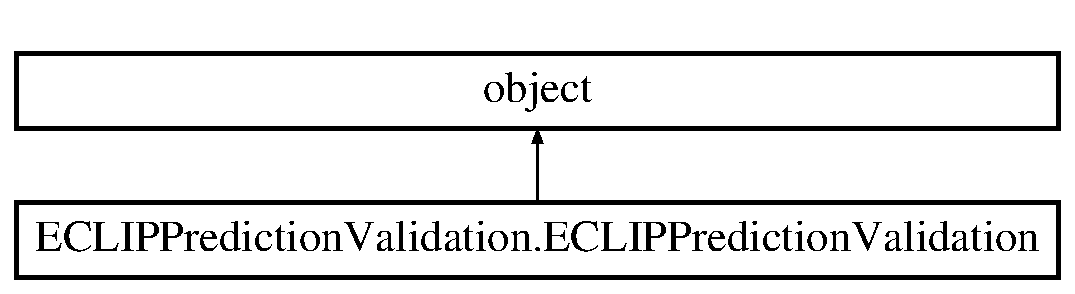
\includegraphics[height=2.000000cm]{classECLIPPredictionValidation_1_1ECLIPPredictionValidation}
\end{center}
\end{figure}
\subsection*{Public Member Functions}
\begin{DoxyCompactItemize}
\item 
\hypertarget{classECLIPPredictionValidation_1_1ECLIPPredictionValidation_aa57c31f655660ae5f4fc129d1e9aef06}{def {\bfseries \-\_\-\-\_\-init\-\_\-\-\_\-}}\label{classECLIPPredictionValidation_1_1ECLIPPredictionValidation_aa57c31f655660ae5f4fc129d1e9aef06}

\item 
\hypertarget{classECLIPPredictionValidation_1_1ECLIPPredictionValidation_a1533429475fb477e4f91b0b8bc8ed832}{def {\bfseries read\-\_\-eclip\-\_\-file}}\label{classECLIPPredictionValidation_1_1ECLIPPredictionValidation_a1533429475fb477e4f91b0b8bc8ed832}

\item 
\hypertarget{classECLIPPredictionValidation_1_1ECLIPPredictionValidation_af30c5de1c6e5381ff9bd6c5a4e5de979}{def {\bfseries read\-\_\-catrapid\-\_\-file}}\label{classECLIPPredictionValidation_1_1ECLIPPredictionValidation_af30c5de1c6e5381ff9bd6c5a4e5de979}

\end{DoxyCompactItemize}
\subsection*{Public Attributes}
\begin{DoxyCompactItemize}
\item 
\hypertarget{classECLIPPredictionValidation_1_1ECLIPPredictionValidation_a7d09ab57e6ffeb21545afb5a3972b43f}{{\bfseries catrapid\-File}}\label{classECLIPPredictionValidation_1_1ECLIPPredictionValidation_a7d09ab57e6ffeb21545afb5a3972b43f}

\item 
\hypertarget{classECLIPPredictionValidation_1_1ECLIPPredictionValidation_a4e79e09a3a3bef3e32f0492a054c6372}{{\bfseries e\-Clip\-File}}\label{classECLIPPredictionValidation_1_1ECLIPPredictionValidation_a4e79e09a3a3bef3e32f0492a054c6372}

\item 
\hypertarget{classECLIPPredictionValidation_1_1ECLIPPredictionValidation_a07208ba0be44716018524339ffa4a2ae}{{\bfseries output\-Folder}}\label{classECLIPPredictionValidation_1_1ECLIPPredictionValidation_a07208ba0be44716018524339ffa4a2ae}

\item 
\hypertarget{classECLIPPredictionValidation_1_1ECLIPPredictionValidation_a1f479aaee98516859304e14d5b66cc97}{{\bfseries eclip\-Pairs}}\label{classECLIPPredictionValidation_1_1ECLIPPredictionValidation_a1f479aaee98516859304e14d5b66cc97}

\end{DoxyCompactItemize}


The documentation for this class was generated from the following file\-:\begin{DoxyCompactItemize}
\item 
src/fr/tagc/rainet/core/execution/processing/known\-Scaffold\-Examples/e\-C\-L\-I\-P/E\-C\-L\-I\-P\-Prediction\-Validation.\-py\end{DoxyCompactItemize}

\hypertarget{classsrc_1_1fr_1_1tagc_1_1rainet_1_1core_1_1execution_1_1analysis_1_1EnrichmentAnalysis_1_1Enric6c627eb5bd04b7c51c1ec93bc189786a}{\section{src.\-fr.\-tagc.\-rainet.\-core.\-execution.\-analysis.\-Enrichment\-Analysis.\-Enrichment2\-Protein.\-Enrichment2\-Protein Class Reference}
\label{classsrc_1_1fr_1_1tagc_1_1rainet_1_1core_1_1execution_1_1analysis_1_1EnrichmentAnalysis_1_1Enric6c627eb5bd04b7c51c1ec93bc189786a}\index{src.\-fr.\-tagc.\-rainet.\-core.\-execution.\-analysis.\-Enrichment\-Analysis.\-Enrichment2\-Protein.\-Enrichment2\-Protein@{src.\-fr.\-tagc.\-rainet.\-core.\-execution.\-analysis.\-Enrichment\-Analysis.\-Enrichment2\-Protein.\-Enrichment2\-Protein}}
}
Inheritance diagram for src.\-fr.\-tagc.\-rainet.\-core.\-execution.\-analysis.\-Enrichment\-Analysis.\-Enrichment2\-Protein.\-Enrichment2\-Protein\-:\begin{figure}[H]
\begin{center}
\leavevmode
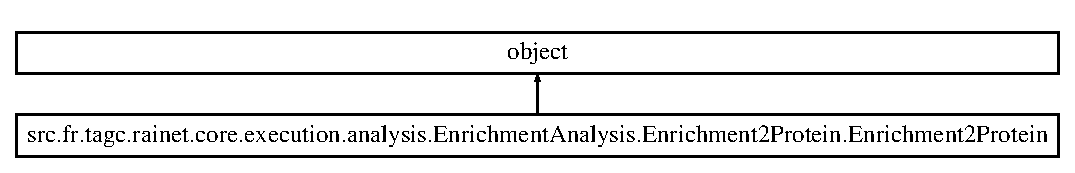
\includegraphics[height=1.879195cm]{classsrc_1_1fr_1_1tagc_1_1rainet_1_1core_1_1execution_1_1analysis_1_1EnrichmentAnalysis_1_1Enric6c627eb5bd04b7c51c1ec93bc189786a}
\end{center}
\end{figure}
\subsection*{Public Member Functions}
\begin{DoxyCompactItemize}
\item 
\hypertarget{classsrc_1_1fr_1_1tagc_1_1rainet_1_1core_1_1execution_1_1analysis_1_1EnrichmentAnalysis_1_1Enric6c627eb5bd04b7c51c1ec93bc189786a_a1be0a364076142bad1ac99ea0f670309}{def {\bfseries \-\_\-\-\_\-init\-\_\-\-\_\-}}\label{classsrc_1_1fr_1_1tagc_1_1rainet_1_1core_1_1execution_1_1analysis_1_1EnrichmentAnalysis_1_1Enric6c627eb5bd04b7c51c1ec93bc189786a_a1be0a364076142bad1ac99ea0f670309}

\item 
\hypertarget{classsrc_1_1fr_1_1tagc_1_1rainet_1_1core_1_1execution_1_1analysis_1_1EnrichmentAnalysis_1_1Enric6c627eb5bd04b7c51c1ec93bc189786a_a4667bab183dd472928105b6b144ef0e0}{def {\bfseries read\-\_\-rainet\-\_\-db}}\label{classsrc_1_1fr_1_1tagc_1_1rainet_1_1core_1_1execution_1_1analysis_1_1EnrichmentAnalysis_1_1Enric6c627eb5bd04b7c51c1ec93bc189786a_a4667bab183dd472928105b6b144ef0e0}

\item 
\hypertarget{classsrc_1_1fr_1_1tagc_1_1rainet_1_1core_1_1execution_1_1analysis_1_1EnrichmentAnalysis_1_1Enric6c627eb5bd04b7c51c1ec93bc189786a_a7fd174cbbd04e5b27f9f74c227e0237a}{def {\bfseries read\-\_\-enrichment\-\_\-data}}\label{classsrc_1_1fr_1_1tagc_1_1rainet_1_1core_1_1execution_1_1analysis_1_1EnrichmentAnalysis_1_1Enric6c627eb5bd04b7c51c1ec93bc189786a_a7fd174cbbd04e5b27f9f74c227e0237a}

\item 
\hypertarget{classsrc_1_1fr_1_1tagc_1_1rainet_1_1core_1_1execution_1_1analysis_1_1EnrichmentAnalysis_1_1Enric6c627eb5bd04b7c51c1ec93bc189786a_a7e8877f1898f509a65087ed33cc3f7dc}{def {\bfseries run}}\label{classsrc_1_1fr_1_1tagc_1_1rainet_1_1core_1_1execution_1_1analysis_1_1EnrichmentAnalysis_1_1Enric6c627eb5bd04b7c51c1ec93bc189786a_a7e8877f1898f509a65087ed33cc3f7dc}

\end{DoxyCompactItemize}
\subsection*{Public Attributes}
\begin{DoxyCompactItemize}
\item 
\hypertarget{classsrc_1_1fr_1_1tagc_1_1rainet_1_1core_1_1execution_1_1analysis_1_1EnrichmentAnalysis_1_1Enric6c627eb5bd04b7c51c1ec93bc189786a_a5927a012153128db7efd7e47e86e8d7f}{{\bfseries rainet\-D\-B}}\label{classsrc_1_1fr_1_1tagc_1_1rainet_1_1core_1_1execution_1_1analysis_1_1EnrichmentAnalysis_1_1Enric6c627eb5bd04b7c51c1ec93bc189786a_a5927a012153128db7efd7e47e86e8d7f}

\item 
\hypertarget{classsrc_1_1fr_1_1tagc_1_1rainet_1_1core_1_1execution_1_1analysis_1_1EnrichmentAnalysis_1_1Enric6c627eb5bd04b7c51c1ec93bc189786a_ad07512adb924a6535a3452f1786ee2e5}{{\bfseries enrichment\-Data}}\label{classsrc_1_1fr_1_1tagc_1_1rainet_1_1core_1_1execution_1_1analysis_1_1EnrichmentAnalysis_1_1Enric6c627eb5bd04b7c51c1ec93bc189786a_ad07512adb924a6535a3452f1786ee2e5}

\item 
\hypertarget{classsrc_1_1fr_1_1tagc_1_1rainet_1_1core_1_1execution_1_1analysis_1_1EnrichmentAnalysis_1_1Enric6c627eb5bd04b7c51c1ec93bc189786a_aaacf886634ba9185f5a9526809236e02}{{\bfseries output\-Folder}}\label{classsrc_1_1fr_1_1tagc_1_1rainet_1_1core_1_1execution_1_1analysis_1_1EnrichmentAnalysis_1_1Enric6c627eb5bd04b7c51c1ec93bc189786a_aaacf886634ba9185f5a9526809236e02}

\item 
\hypertarget{classsrc_1_1fr_1_1tagc_1_1rainet_1_1core_1_1execution_1_1analysis_1_1EnrichmentAnalysis_1_1Enric6c627eb5bd04b7c51c1ec93bc189786a_a486b0e7d0fbd5a2db2b4d476c6d1d066}{{\bfseries complex\-Datasets}}\label{classsrc_1_1fr_1_1tagc_1_1rainet_1_1core_1_1execution_1_1analysis_1_1EnrichmentAnalysis_1_1Enric6c627eb5bd04b7c51c1ec93bc189786a_a486b0e7d0fbd5a2db2b4d476c6d1d066}

\item 
\hypertarget{classsrc_1_1fr_1_1tagc_1_1rainet_1_1core_1_1execution_1_1analysis_1_1EnrichmentAnalysis_1_1Enric6c627eb5bd04b7c51c1ec93bc189786a_abe38a56b32aa9e27a133c3f0bbdebf32}{{\bfseries sql\-\_\-session}}\label{classsrc_1_1fr_1_1tagc_1_1rainet_1_1core_1_1execution_1_1analysis_1_1EnrichmentAnalysis_1_1Enric6c627eb5bd04b7c51c1ec93bc189786a_abe38a56b32aa9e27a133c3f0bbdebf32}

\item 
\hypertarget{classsrc_1_1fr_1_1tagc_1_1rainet_1_1core_1_1execution_1_1analysis_1_1EnrichmentAnalysis_1_1Enric6c627eb5bd04b7c51c1ec93bc189786a_a53ef77918526e86a8ea4d77b111b8724}{{\bfseries complex\-Data}}\label{classsrc_1_1fr_1_1tagc_1_1rainet_1_1core_1_1execution_1_1analysis_1_1EnrichmentAnalysis_1_1Enric6c627eb5bd04b7c51c1ec93bc189786a_a53ef77918526e86a8ea4d77b111b8724}

\end{DoxyCompactItemize}
\subsection*{Static Public Attributes}
\begin{DoxyCompactItemize}
\item 
\hypertarget{classsrc_1_1fr_1_1tagc_1_1rainet_1_1core_1_1execution_1_1analysis_1_1EnrichmentAnalysis_1_1Enric6c627eb5bd04b7c51c1ec93bc189786a_a5beeb137b8d3dd53c1c15130e4f446db}{string {\bfseries O\-U\-T\-P\-U\-T\-\_\-\-F\-I\-L\-E\-\_\-1} = \char`\"{}/enrichment\-\_\-results\-\_\-with\-\_\-protein\-\_\-ids.\-txt\char`\"{}}\label{classsrc_1_1fr_1_1tagc_1_1rainet_1_1core_1_1execution_1_1analysis_1_1EnrichmentAnalysis_1_1Enric6c627eb5bd04b7c51c1ec93bc189786a_a5beeb137b8d3dd53c1c15130e4f446db}

\item 
\hypertarget{classsrc_1_1fr_1_1tagc_1_1rainet_1_1core_1_1execution_1_1analysis_1_1EnrichmentAnalysis_1_1Enric6c627eb5bd04b7c51c1ec93bc189786a_a758cd20688656a2777b887bef997b8db}{string {\bfseries O\-U\-T\-P\-U\-T\-\_\-\-F\-I\-L\-E\-\_\-2} = \char`\"{}/transcript\-\_\-ids\-\_\-associated\-\_\-protein\-\_\-ids.\-txt\char`\"{}}\label{classsrc_1_1fr_1_1tagc_1_1rainet_1_1core_1_1execution_1_1analysis_1_1EnrichmentAnalysis_1_1Enric6c627eb5bd04b7c51c1ec93bc189786a_a758cd20688656a2777b887bef997b8db}

\item 
dictionary {\bfseries A\-N\-N\-O\-T\-A\-T\-I\-O\-N\-\_\-\-T\-A\-B\-L\-E\-S\-\_\-\-D\-I\-C\-T}
\end{DoxyCompactItemize}


\subsection{Member Data Documentation}
\hypertarget{classsrc_1_1fr_1_1tagc_1_1rainet_1_1core_1_1execution_1_1analysis_1_1EnrichmentAnalysis_1_1Enric6c627eb5bd04b7c51c1ec93bc189786a_a9e4991e3f642f90ca9faf554e59c8301}{\index{src\-::fr\-::tagc\-::rainet\-::core\-::execution\-::analysis\-::\-Enrichment\-Analysis\-::\-Enrichment2\-Protein\-::\-Enrichment2\-Protein@{src\-::fr\-::tagc\-::rainet\-::core\-::execution\-::analysis\-::\-Enrichment\-Analysis\-::\-Enrichment2\-Protein\-::\-Enrichment2\-Protein}!A\-N\-N\-O\-T\-A\-T\-I\-O\-N\-\_\-\-T\-A\-B\-L\-E\-S\-\_\-\-D\-I\-C\-T@{A\-N\-N\-O\-T\-A\-T\-I\-O\-N\-\_\-\-T\-A\-B\-L\-E\-S\-\_\-\-D\-I\-C\-T}}
\index{A\-N\-N\-O\-T\-A\-T\-I\-O\-N\-\_\-\-T\-A\-B\-L\-E\-S\-\_\-\-D\-I\-C\-T@{A\-N\-N\-O\-T\-A\-T\-I\-O\-N\-\_\-\-T\-A\-B\-L\-E\-S\-\_\-\-D\-I\-C\-T}!src::fr::tagc::rainet::core::execution::analysis::EnrichmentAnalysis::Enrichment2Protein::Enrichment2Protein@{src\-::fr\-::tagc\-::rainet\-::core\-::execution\-::analysis\-::\-Enrichment\-Analysis\-::\-Enrichment2\-Protein\-::\-Enrichment2\-Protein}}
\subsubsection[{A\-N\-N\-O\-T\-A\-T\-I\-O\-N\-\_\-\-T\-A\-B\-L\-E\-S\-\_\-\-D\-I\-C\-T}]{\setlength{\rightskip}{0pt plus 5cm}dictionary src.\-fr.\-tagc.\-rainet.\-core.\-execution.\-analysis.\-Enrichment\-Analysis.\-Enrichment2\-Protein.\-Enrichment2\-Protein.\-A\-N\-N\-O\-T\-A\-T\-I\-O\-N\-\_\-\-T\-A\-B\-L\-E\-S\-\_\-\-D\-I\-C\-T\hspace{0.3cm}{\ttfamily [static]}}}\label{classsrc_1_1fr_1_1tagc_1_1rainet_1_1core_1_1execution_1_1analysis_1_1EnrichmentAnalysis_1_1Enric6c627eb5bd04b7c51c1ec93bc189786a_a9e4991e3f642f90ca9faf554e59c8301}
{\bfseries Initial value\-:}
\begin{DoxyCode}
1 = \{\textcolor{stringliteral}{"NetworkModule"} : \textcolor{stringliteral}{"ProteinNetworkModule"},
2                               \textcolor{stringliteral}{"ReactomePathway"} : \textcolor{stringliteral}{"ProteinReactomeAnnotation"},
3                               \textcolor{stringliteral}{"KEGGPathway"} : \textcolor{stringliteral}{"ProteinKEGGAnnotation"},
4                               \textcolor{stringliteral}{"BioplexCluster"} : \textcolor{stringliteral}{"ProteinBioplexAnnotation"},
5                               \textcolor{stringliteral}{"WanCluster"} : \textcolor{stringliteral}{"ProteinWanAnnotation"},
6                               \textcolor{stringliteral}{"CorumCluster"} : \textcolor{stringliteral}{"ProteinCorumAnnotation"},
7                               \textcolor{stringliteral}{"CustomCluster"} : \textcolor{stringliteral}{"ProteinCustomAnnotation"}\}
\end{DoxyCode}


The documentation for this class was generated from the following file\-:\begin{DoxyCompactItemize}
\item 
src/fr/tagc/rainet/core/execution/analysis/\-Enrichment\-Analysis/Enrichment2\-Protein.\-py\end{DoxyCompactItemize}

\hypertarget{classsrc_1_1fr_1_1tagc_1_1rainet_1_1core_1_1execution_1_1EnrichmentAnalysisStategy_1_1EnrichmentAnalysisStrategy}{\section{src.\-fr.\-tagc.\-rainet.\-core.\-execution.\-Enrichment\-Analysis\-Stategy.\-Enrichment\-Analysis\-Strategy Class Reference}
\label{classsrc_1_1fr_1_1tagc_1_1rainet_1_1core_1_1execution_1_1EnrichmentAnalysisStategy_1_1EnrichmentAnalysisStrategy}\index{src.\-fr.\-tagc.\-rainet.\-core.\-execution.\-Enrichment\-Analysis\-Stategy.\-Enrichment\-Analysis\-Strategy@{src.\-fr.\-tagc.\-rainet.\-core.\-execution.\-Enrichment\-Analysis\-Stategy.\-Enrichment\-Analysis\-Strategy}}
}
Inheritance diagram for src.\-fr.\-tagc.\-rainet.\-core.\-execution.\-Enrichment\-Analysis\-Stategy.\-Enrichment\-Analysis\-Strategy\-:\begin{figure}[H]
\begin{center}
\leavevmode
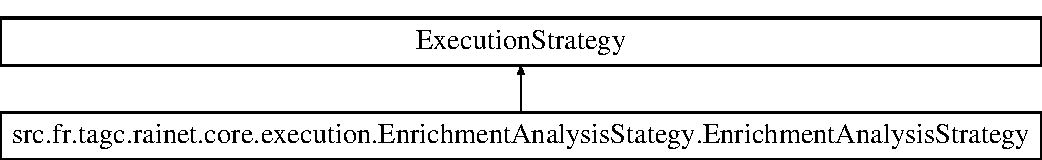
\includegraphics[height=2.000000cm]{classsrc_1_1fr_1_1tagc_1_1rainet_1_1core_1_1execution_1_1EnrichmentAnalysisStategy_1_1EnrichmentAnalysisStrategy}
\end{center}
\end{figure}
\subsection*{Public Member Functions}
\begin{DoxyCompactItemize}
\item 
\hypertarget{classsrc_1_1fr_1_1tagc_1_1rainet_1_1core_1_1execution_1_1EnrichmentAnalysisStategy_1_1EnrichmentAnalysisStrategy_a141a2100ae61206bf6358dc3566ff34f}{def {\bfseries \-\_\-\-\_\-init\-\_\-\-\_\-}}\label{classsrc_1_1fr_1_1tagc_1_1rainet_1_1core_1_1execution_1_1EnrichmentAnalysisStategy_1_1EnrichmentAnalysisStrategy_a141a2100ae61206bf6358dc3566ff34f}

\item 
\hypertarget{classsrc_1_1fr_1_1tagc_1_1rainet_1_1core_1_1execution_1_1EnrichmentAnalysisStategy_1_1EnrichmentAnalysisStrategy_af8bec79c8bc3155f7918970f3143dfb1}{def {\bfseries execute}}\label{classsrc_1_1fr_1_1tagc_1_1rainet_1_1core_1_1execution_1_1EnrichmentAnalysisStategy_1_1EnrichmentAnalysisStrategy_af8bec79c8bc3155f7918970f3143dfb1}

\item 
\hypertarget{classsrc_1_1fr_1_1tagc_1_1rainet_1_1core_1_1execution_1_1EnrichmentAnalysisStategy_1_1EnrichmentAnalysisStrategy_a95f160205be6fc8fb9b3c56546a7c553}{def {\bfseries analysis}}\label{classsrc_1_1fr_1_1tagc_1_1rainet_1_1core_1_1execution_1_1EnrichmentAnalysisStategy_1_1EnrichmentAnalysisStrategy_a95f160205be6fc8fb9b3c56546a7c553}

\item 
\hypertarget{classsrc_1_1fr_1_1tagc_1_1rainet_1_1core_1_1execution_1_1EnrichmentAnalysisStategy_1_1EnrichmentAnalysisStrategy_aeda6819294e8776d4f311227aac3fb8e}{def {\bfseries write\-\_\-parameter\-\_\-log}}\label{classsrc_1_1fr_1_1tagc_1_1rainet_1_1core_1_1execution_1_1EnrichmentAnalysisStategy_1_1EnrichmentAnalysisStrategy_aeda6819294e8776d4f311227aac3fb8e}

\item 
\hypertarget{classsrc_1_1fr_1_1tagc_1_1rainet_1_1core_1_1execution_1_1EnrichmentAnalysisStategy_1_1EnrichmentAnalysisStrategy_ae2109dba8184f45f855227be6ec9a27f}{def {\bfseries get\-\_\-interaction\-\_\-data}}\label{classsrc_1_1fr_1_1tagc_1_1rainet_1_1core_1_1execution_1_1EnrichmentAnalysisStategy_1_1EnrichmentAnalysisStrategy_ae2109dba8184f45f855227be6ec9a27f}

\item 
\hypertarget{classsrc_1_1fr_1_1tagc_1_1rainet_1_1core_1_1execution_1_1EnrichmentAnalysisStategy_1_1EnrichmentAnalysisStrategy_ac350f345dfccfb14c71d4baf55c35065}{def {\bfseries annotation\-\_\-report}}\label{classsrc_1_1fr_1_1tagc_1_1rainet_1_1core_1_1execution_1_1EnrichmentAnalysisStategy_1_1EnrichmentAnalysisStrategy_ac350f345dfccfb14c71d4baf55c35065}

\item 
\hypertarget{classsrc_1_1fr_1_1tagc_1_1rainet_1_1core_1_1execution_1_1EnrichmentAnalysisStategy_1_1EnrichmentAnalysisStrategy_acb5e88fb889813498dcba227ed091d85}{def {\bfseries enrichement\-\_\-analysis}}\label{classsrc_1_1fr_1_1tagc_1_1rainet_1_1core_1_1execution_1_1EnrichmentAnalysisStategy_1_1EnrichmentAnalysisStrategy_acb5e88fb889813498dcba227ed091d85}

\item 
\hypertarget{classsrc_1_1fr_1_1tagc_1_1rainet_1_1core_1_1execution_1_1EnrichmentAnalysisStategy_1_1EnrichmentAnalysisStrategy_aef8d8df30a33b38e2bc5dbab6aefc56a}{def {\bfseries run\-\_\-rna\-\_\-vs\-\_\-annotations}}\label{classsrc_1_1fr_1_1tagc_1_1rainet_1_1core_1_1execution_1_1EnrichmentAnalysisStategy_1_1EnrichmentAnalysisStrategy_aef8d8df30a33b38e2bc5dbab6aefc56a}

\item 
\hypertarget{classsrc_1_1fr_1_1tagc_1_1rainet_1_1core_1_1execution_1_1EnrichmentAnalysisStategy_1_1EnrichmentAnalysisStrategy_a1294116655fbabfa2d6c639621e37237}{def {\bfseries correct\-\_\-pvalues}}\label{classsrc_1_1fr_1_1tagc_1_1rainet_1_1core_1_1execution_1_1EnrichmentAnalysisStategy_1_1EnrichmentAnalysisStrategy_a1294116655fbabfa2d6c639621e37237}

\item 
\hypertarget{classsrc_1_1fr_1_1tagc_1_1rainet_1_1core_1_1execution_1_1EnrichmentAnalysisStategy_1_1EnrichmentAnalysisStrategy_a99b8a81f1d96208828eb4647d8cdd5c5}{def {\bfseries multiple\-\_\-test\-\_\-correction}}\label{classsrc_1_1fr_1_1tagc_1_1rainet_1_1core_1_1execution_1_1EnrichmentAnalysisStategy_1_1EnrichmentAnalysisStrategy_a99b8a81f1d96208828eb4647d8cdd5c5}

\item 
\hypertarget{classsrc_1_1fr_1_1tagc_1_1rainet_1_1core_1_1execution_1_1EnrichmentAnalysisStategy_1_1EnrichmentAnalysisStrategy_a0b288558090574cf741574f48a5b2c3f}{def {\bfseries hypergeometric\-\_\-test}}\label{classsrc_1_1fr_1_1tagc_1_1rainet_1_1core_1_1execution_1_1EnrichmentAnalysisStategy_1_1EnrichmentAnalysisStrategy_a0b288558090574cf741574f48a5b2c3f}

\item 
\hypertarget{classsrc_1_1fr_1_1tagc_1_1rainet_1_1core_1_1execution_1_1EnrichmentAnalysisStategy_1_1EnrichmentAnalysisStrategy_a7d2e88b37cb0a310c2acdacb0dd8249e}{def {\bfseries count\-\_\-sign\-\_\-tests}}\label{classsrc_1_1fr_1_1tagc_1_1rainet_1_1core_1_1execution_1_1EnrichmentAnalysisStategy_1_1EnrichmentAnalysisStrategy_a7d2e88b37cb0a310c2acdacb0dd8249e}

\item 
\hypertarget{classsrc_1_1fr_1_1tagc_1_1rainet_1_1core_1_1execution_1_1EnrichmentAnalysisStategy_1_1EnrichmentAnalysisStrategy_a9527f3d43655ca772c765acbaac251ae}{def {\bfseries empirical\-\_\-pvalue}}\label{classsrc_1_1fr_1_1tagc_1_1rainet_1_1core_1_1execution_1_1EnrichmentAnalysisStategy_1_1EnrichmentAnalysisStrategy_a9527f3d43655ca772c765acbaac251ae}

\item 
\hypertarget{classsrc_1_1fr_1_1tagc_1_1rainet_1_1core_1_1execution_1_1EnrichmentAnalysisStategy_1_1EnrichmentAnalysisStrategy_a7a4367f81925d12fa5021420d5905ec9}{def {\bfseries randomize\-\_\-annotation}}\label{classsrc_1_1fr_1_1tagc_1_1rainet_1_1core_1_1execution_1_1EnrichmentAnalysisStategy_1_1EnrichmentAnalysisStrategy_a7a4367f81925d12fa5021420d5905ec9}

\item 
\hypertarget{classsrc_1_1fr_1_1tagc_1_1rainet_1_1core_1_1execution_1_1EnrichmentAnalysisStategy_1_1EnrichmentAnalysisStrategy_a919b4903a28aa65a91ddb35c875e3ca2}{def {\bfseries randomize\-\_\-proteins}}\label{classsrc_1_1fr_1_1tagc_1_1rainet_1_1core_1_1execution_1_1EnrichmentAnalysisStategy_1_1EnrichmentAnalysisStrategy_a919b4903a28aa65a91ddb35c875e3ca2}

\item 
\hypertarget{classsrc_1_1fr_1_1tagc_1_1rainet_1_1core_1_1execution_1_1EnrichmentAnalysisStategy_1_1EnrichmentAnalysisStrategy_af4ab21864a34fd27895aa6c250d616e9}{def {\bfseries retrieve\-\_\-expression}}\label{classsrc_1_1fr_1_1tagc_1_1rainet_1_1core_1_1execution_1_1EnrichmentAnalysisStategy_1_1EnrichmentAnalysisStrategy_af4ab21864a34fd27895aa6c250d616e9}

\item 
\hypertarget{classsrc_1_1fr_1_1tagc_1_1rainet_1_1core_1_1execution_1_1EnrichmentAnalysisStategy_1_1EnrichmentAnalysisStrategy_a72e864cd5c0da8142fb4c469b478f1d0}{def {\bfseries write\-\_\-report}}\label{classsrc_1_1fr_1_1tagc_1_1rainet_1_1core_1_1execution_1_1EnrichmentAnalysisStategy_1_1EnrichmentAnalysisStrategy_a72e864cd5c0da8142fb4c469b478f1d0}

\end{DoxyCompactItemize}
\subsection*{Public Attributes}
\begin{DoxyCompactItemize}
\item 
\hypertarget{classsrc_1_1fr_1_1tagc_1_1rainet_1_1core_1_1execution_1_1EnrichmentAnalysisStategy_1_1EnrichmentAnalysisStrategy_a185fc6092eeb3b7503a319b919654b55}{{\bfseries write\-Report\-File}}\label{classsrc_1_1fr_1_1tagc_1_1rainet_1_1core_1_1execution_1_1EnrichmentAnalysisStategy_1_1EnrichmentAnalysisStrategy_a185fc6092eeb3b7503a319b919654b55}

\item 
\hypertarget{classsrc_1_1fr_1_1tagc_1_1rainet_1_1core_1_1execution_1_1EnrichmentAnalysisStategy_1_1EnrichmentAnalysisStrategy_a2811a6ecff6a95498865635d328c957e}{{\bfseries test\-Container}}\label{classsrc_1_1fr_1_1tagc_1_1rainet_1_1core_1_1execution_1_1EnrichmentAnalysisStategy_1_1EnrichmentAnalysisStrategy_a2811a6ecff6a95498865635d328c957e}

\item 
\hypertarget{classsrc_1_1fr_1_1tagc_1_1rainet_1_1core_1_1execution_1_1EnrichmentAnalysisStategy_1_1EnrichmentAnalysisStrategy_a3262d4c1a4459fc23bd34f13698a1894}{{\bfseries count\-Total\-Tests}}\label{classsrc_1_1fr_1_1tagc_1_1rainet_1_1core_1_1execution_1_1EnrichmentAnalysisStategy_1_1EnrichmentAnalysisStrategy_a3262d4c1a4459fc23bd34f13698a1894}

\item 
\hypertarget{classsrc_1_1fr_1_1tagc_1_1rainet_1_1core_1_1execution_1_1EnrichmentAnalysisStategy_1_1EnrichmentAnalysisStrategy_aa8bd40e0a1538c8778cc509216a56d94}{{\bfseries D\-B\-Path}}\label{classsrc_1_1fr_1_1tagc_1_1rainet_1_1core_1_1execution_1_1EnrichmentAnalysisStategy_1_1EnrichmentAnalysisStrategy_aa8bd40e0a1538c8778cc509216a56d94}

\item 
\hypertarget{classsrc_1_1fr_1_1tagc_1_1rainet_1_1core_1_1execution_1_1EnrichmentAnalysisStategy_1_1EnrichmentAnalysisStrategy_a3637ea939c66beaa3bf39c1473b2c01e}{{\bfseries species}}\label{classsrc_1_1fr_1_1tagc_1_1rainet_1_1core_1_1execution_1_1EnrichmentAnalysisStategy_1_1EnrichmentAnalysisStrategy_a3637ea939c66beaa3bf39c1473b2c01e}

\item 
\hypertarget{classsrc_1_1fr_1_1tagc_1_1rainet_1_1core_1_1execution_1_1EnrichmentAnalysisStategy_1_1EnrichmentAnalysisStrategy_a38ad1c83d7f08a13b658434bd5f40fe7}{{\bfseries output\-Folder}}\label{classsrc_1_1fr_1_1tagc_1_1rainet_1_1core_1_1execution_1_1EnrichmentAnalysisStategy_1_1EnrichmentAnalysisStrategy_a38ad1c83d7f08a13b658434bd5f40fe7}

\item 
\hypertarget{classsrc_1_1fr_1_1tagc_1_1rainet_1_1core_1_1execution_1_1EnrichmentAnalysisStategy_1_1EnrichmentAnalysisStrategy_af1c45e8b71159e45a49255271027a007}{{\bfseries annotation\-Table}}\label{classsrc_1_1fr_1_1tagc_1_1rainet_1_1core_1_1execution_1_1EnrichmentAnalysisStategy_1_1EnrichmentAnalysisStrategy_af1c45e8b71159e45a49255271027a007}

\item 
\hypertarget{classsrc_1_1fr_1_1tagc_1_1rainet_1_1core_1_1execution_1_1EnrichmentAnalysisStategy_1_1EnrichmentAnalysisStrategy_a3090c943e6ef603d43cb643892211d98}{{\bfseries minimum\-Protein\-Annotation}}\label{classsrc_1_1fr_1_1tagc_1_1rainet_1_1core_1_1execution_1_1EnrichmentAnalysisStategy_1_1EnrichmentAnalysisStrategy_a3090c943e6ef603d43cb643892211d98}

\item 
\hypertarget{classsrc_1_1fr_1_1tagc_1_1rainet_1_1core_1_1execution_1_1EnrichmentAnalysisStategy_1_1EnrichmentAnalysisStrategy_ae854959533174390cc74f3aab1e99066}{{\bfseries minimum\-Protein\-Interaction}}\label{classsrc_1_1fr_1_1tagc_1_1rainet_1_1core_1_1execution_1_1EnrichmentAnalysisStategy_1_1EnrichmentAnalysisStrategy_ae854959533174390cc74f3aab1e99066}

\item 
\hypertarget{classsrc_1_1fr_1_1tagc_1_1rainet_1_1core_1_1execution_1_1EnrichmentAnalysisStategy_1_1EnrichmentAnalysisStrategy_a4717c09374108b7342ebc0ad90be181a}{{\bfseries number\-Randomizations}}\label{classsrc_1_1fr_1_1tagc_1_1rainet_1_1core_1_1execution_1_1EnrichmentAnalysisStategy_1_1EnrichmentAnalysisStrategy_a4717c09374108b7342ebc0ad90be181a}

\item 
\hypertarget{classsrc_1_1fr_1_1tagc_1_1rainet_1_1core_1_1execution_1_1EnrichmentAnalysisStategy_1_1EnrichmentAnalysisStrategy_a57704811d01042f85d04565ad5df30bd}{{\bfseries expression\-Warning}}\label{classsrc_1_1fr_1_1tagc_1_1rainet_1_1core_1_1execution_1_1EnrichmentAnalysisStategy_1_1EnrichmentAnalysisStrategy_a57704811d01042f85d04565ad5df30bd}

\item 
\hypertarget{classsrc_1_1fr_1_1tagc_1_1rainet_1_1core_1_1execution_1_1EnrichmentAnalysisStategy_1_1EnrichmentAnalysisStrategy_aae974c41ca4ab6ca0ae17d48c0555645}{{\bfseries minimum\-Expression}}\label{classsrc_1_1fr_1_1tagc_1_1rainet_1_1core_1_1execution_1_1EnrichmentAnalysisStategy_1_1EnrichmentAnalysisStrategy_aae974c41ca4ab6ca0ae17d48c0555645}

\item 
\hypertarget{classsrc_1_1fr_1_1tagc_1_1rainet_1_1core_1_1execution_1_1EnrichmentAnalysisStategy_1_1EnrichmentAnalysisStrategy_ac2bc3f0d61e85f614d6112d37be0886b}{{\bfseries lower\-Tail}}\label{classsrc_1_1fr_1_1tagc_1_1rainet_1_1core_1_1execution_1_1EnrichmentAnalysisStategy_1_1EnrichmentAnalysisStrategy_ac2bc3f0d61e85f614d6112d37be0886b}

\item 
\hypertarget{classsrc_1_1fr_1_1tagc_1_1rainet_1_1core_1_1execution_1_1EnrichmentAnalysisStategy_1_1EnrichmentAnalysisStrategy_a6e76fe947d886c29d480acbcd94fb7c4}{{\bfseries arguments}}\label{classsrc_1_1fr_1_1tagc_1_1rainet_1_1core_1_1execution_1_1EnrichmentAnalysisStategy_1_1EnrichmentAnalysisStrategy_a6e76fe947d886c29d480acbcd94fb7c4}

\item 
\hypertarget{classsrc_1_1fr_1_1tagc_1_1rainet_1_1core_1_1execution_1_1EnrichmentAnalysisStategy_1_1EnrichmentAnalysisStrategy_a99f34710a657fb9c1ab4b2578ab9570e}{{\bfseries sql\-\_\-session}}\label{classsrc_1_1fr_1_1tagc_1_1rainet_1_1core_1_1execution_1_1EnrichmentAnalysisStategy_1_1EnrichmentAnalysisStrategy_a99f34710a657fb9c1ab4b2578ab9570e}

\item 
\hypertarget{classsrc_1_1fr_1_1tagc_1_1rainet_1_1core_1_1execution_1_1EnrichmentAnalysisStategy_1_1EnrichmentAnalysisStrategy_afcce34a604687069876e8c0f5321bf4e}{{\bfseries db\-\_\-engine}}\label{classsrc_1_1fr_1_1tagc_1_1rainet_1_1core_1_1execution_1_1EnrichmentAnalysisStategy_1_1EnrichmentAnalysisStrategy_afcce34a604687069876e8c0f5321bf4e}

\item 
\hypertarget{classsrc_1_1fr_1_1tagc_1_1rainet_1_1core_1_1execution_1_1EnrichmentAnalysisStategy_1_1EnrichmentAnalysisStrategy_a2264cd92d04571939763ab8906baf280}{{\bfseries prot\-Annot\-Dict}}\label{classsrc_1_1fr_1_1tagc_1_1rainet_1_1core_1_1execution_1_1EnrichmentAnalysisStategy_1_1EnrichmentAnalysisStrategy_a2264cd92d04571939763ab8906baf280}

\item 
\hypertarget{classsrc_1_1fr_1_1tagc_1_1rainet_1_1core_1_1execution_1_1EnrichmentAnalysisStategy_1_1EnrichmentAnalysisStrategy_a5daeaa5fa182db146e650c50d977b5df}{{\bfseries annot\-With\-Interaction\-Dict}}\label{classsrc_1_1fr_1_1tagc_1_1rainet_1_1core_1_1execution_1_1EnrichmentAnalysisStategy_1_1EnrichmentAnalysisStrategy_a5daeaa5fa182db146e650c50d977b5df}

\item 
\hypertarget{classsrc_1_1fr_1_1tagc_1_1rainet_1_1core_1_1execution_1_1EnrichmentAnalysisStategy_1_1EnrichmentAnalysisStrategy_a68a436215153287ef08c15bd96e7e23a}{{\bfseries all\-Proteins\-With\-Interaction\-Data\-Len}}\label{classsrc_1_1fr_1_1tagc_1_1rainet_1_1core_1_1execution_1_1EnrichmentAnalysisStategy_1_1EnrichmentAnalysisStrategy_a68a436215153287ef08c15bd96e7e23a}

\item 
\hypertarget{classsrc_1_1fr_1_1tagc_1_1rainet_1_1core_1_1execution_1_1EnrichmentAnalysisStategy_1_1EnrichmentAnalysisStrategy_ae212d786f7861e6e4899db3842062506}{{\bfseries protein\-With\-Annotation\-With\-Interaction}}\label{classsrc_1_1fr_1_1tagc_1_1rainet_1_1core_1_1execution_1_1EnrichmentAnalysisStategy_1_1EnrichmentAnalysisStrategy_ae212d786f7861e6e4899db3842062506}

\item 
\hypertarget{classsrc_1_1fr_1_1tagc_1_1rainet_1_1core_1_1execution_1_1EnrichmentAnalysisStategy_1_1EnrichmentAnalysisStrategy_aea8662e49cdd077a3a370379c5aa2650}{{\bfseries rna\-Interactions\-Length}}\label{classsrc_1_1fr_1_1tagc_1_1rainet_1_1core_1_1execution_1_1EnrichmentAnalysisStategy_1_1EnrichmentAnalysisStrategy_aea8662e49cdd077a3a370379c5aa2650}

\item 
\hypertarget{classsrc_1_1fr_1_1tagc_1_1rainet_1_1core_1_1execution_1_1EnrichmentAnalysisStategy_1_1EnrichmentAnalysisStrategy_a79b2280730f0976826c677a5efd1ee7c}{{\bfseries background\-Proteins}}\label{classsrc_1_1fr_1_1tagc_1_1rainet_1_1core_1_1execution_1_1EnrichmentAnalysisStategy_1_1EnrichmentAnalysisStrategy_a79b2280730f0976826c677a5efd1ee7c}

\item 
\hypertarget{classsrc_1_1fr_1_1tagc_1_1rainet_1_1core_1_1execution_1_1EnrichmentAnalysisStategy_1_1EnrichmentAnalysisStrategy_a167b879fbabe78eb3c11c3c67fdfcdaf}{{\bfseries prot\-Annot\-Dict\-Len}}\label{classsrc_1_1fr_1_1tagc_1_1rainet_1_1core_1_1execution_1_1EnrichmentAnalysisStategy_1_1EnrichmentAnalysisStrategy_a167b879fbabe78eb3c11c3c67fdfcdaf}

\item 
\hypertarget{classsrc_1_1fr_1_1tagc_1_1rainet_1_1core_1_1execution_1_1EnrichmentAnalysisStategy_1_1EnrichmentAnalysisStrategy_a3e95df3ed810011df6acb2fd43cef7ef}{{\bfseries expression\-Dict}}\label{classsrc_1_1fr_1_1tagc_1_1rainet_1_1core_1_1execution_1_1EnrichmentAnalysisStategy_1_1EnrichmentAnalysisStrategy_a3e95df3ed810011df6acb2fd43cef7ef}

\item 
\hypertarget{classsrc_1_1fr_1_1tagc_1_1rainet_1_1core_1_1execution_1_1EnrichmentAnalysisStategy_1_1EnrichmentAnalysisStrategy_ab8868b0694a89600e413cbc584e9bd76}{{\bfseries prot\-Tissue\-Expressions}}\label{classsrc_1_1fr_1_1tagc_1_1rainet_1_1core_1_1execution_1_1EnrichmentAnalysisStategy_1_1EnrichmentAnalysisStrategy_ab8868b0694a89600e413cbc584e9bd76}

\end{DoxyCompactItemize}
\subsection*{Static Public Attributes}
\begin{DoxyCompactItemize}
\item 
dictionary {\bfseries A\-N\-N\-O\-T\-A\-T\-I\-O\-N\-\_\-\-T\-A\-B\-L\-E\-S\-\_\-\-D\-I\-C\-T}
\item 
\hypertarget{classsrc_1_1fr_1_1tagc_1_1rainet_1_1core_1_1execution_1_1EnrichmentAnalysisStategy_1_1EnrichmentAnalysisStrategy_a436ed36f1cfc7eac8342f9b6c73337a0}{float {\bfseries S\-I\-G\-N\-\_\-\-V\-A\-L\-U\-E\-\_\-\-T\-E\-S\-T} = 0.\-05}\label{classsrc_1_1fr_1_1tagc_1_1rainet_1_1core_1_1execution_1_1EnrichmentAnalysisStategy_1_1EnrichmentAnalysisStrategy_a436ed36f1cfc7eac8342f9b6c73337a0}

\item 
\hypertarget{classsrc_1_1fr_1_1tagc_1_1rainet_1_1core_1_1execution_1_1EnrichmentAnalysisStategy_1_1EnrichmentAnalysisStrategy_a22029107b069e432ff74e80e03024f0d}{float {\bfseries S\-I\-G\-N\-\_\-\-V\-A\-L\-U\-E\-\_\-\-A\-G\-A\-I\-N\-S\-T\-\_\-\-R\-A\-N\-D\-O\-M\-\_\-\-C\-O\-N\-T\-R\-O\-L} = 0.\-01}\label{classsrc_1_1fr_1_1tagc_1_1rainet_1_1core_1_1execution_1_1EnrichmentAnalysisStategy_1_1EnrichmentAnalysisStrategy_a22029107b069e432ff74e80e03024f0d}

\item 
\hypertarget{classsrc_1_1fr_1_1tagc_1_1rainet_1_1core_1_1execution_1_1EnrichmentAnalysisStategy_1_1EnrichmentAnalysisStrategy_ae440d8931a8d9e5acade380e84f46293}{int {\bfseries S\-I\-G\-N\-\_\-\-C\-O\-L\-U\-M\-N} = 8}\label{classsrc_1_1fr_1_1tagc_1_1rainet_1_1core_1_1execution_1_1EnrichmentAnalysisStategy_1_1EnrichmentAnalysisStrategy_ae440d8931a8d9e5acade380e84f46293}

\item 
\hypertarget{classsrc_1_1fr_1_1tagc_1_1rainet_1_1core_1_1execution_1_1EnrichmentAnalysisStategy_1_1EnrichmentAnalysisStrategy_aeac1c493397196f53729e9e6a9cfc4a5}{int {\bfseries W\-A\-R\-N\-I\-N\-G\-\_\-\-C\-O\-L\-U\-M\-N} = 5}\label{classsrc_1_1fr_1_1tagc_1_1rainet_1_1core_1_1execution_1_1EnrichmentAnalysisStategy_1_1EnrichmentAnalysisStrategy_aeac1c493397196f53729e9e6a9cfc4a5}

\item 
\hypertarget{classsrc_1_1fr_1_1tagc_1_1rainet_1_1core_1_1execution_1_1EnrichmentAnalysisStategy_1_1EnrichmentAnalysisStrategy_acc35f4adca1f43498cbe308fd9b9e062}{string {\bfseries P\-R\-I\-\_\-\-P\-R\-O\-T\-\_\-\-K\-W} = \char`\"{}interacting\-Proteins\char`\"{}}\label{classsrc_1_1fr_1_1tagc_1_1rainet_1_1core_1_1execution_1_1EnrichmentAnalysisStategy_1_1EnrichmentAnalysisStrategy_acc35f4adca1f43498cbe308fd9b9e062}

\item 
\hypertarget{classsrc_1_1fr_1_1tagc_1_1rainet_1_1core_1_1execution_1_1EnrichmentAnalysisStategy_1_1EnrichmentAnalysisStrategy_a13fe2bebb5d98036016edde4f711e22e}{string {\bfseries P\-R\-I\-\_\-\-R\-N\-A\-\_\-\-K\-W} = \char`\"{}interacting\-R\-N\-As\char`\"{}}\label{classsrc_1_1fr_1_1tagc_1_1rainet_1_1core_1_1execution_1_1EnrichmentAnalysisStategy_1_1EnrichmentAnalysisStrategy_a13fe2bebb5d98036016edde4f711e22e}

\item 
\hypertarget{classsrc_1_1fr_1_1tagc_1_1rainet_1_1core_1_1execution_1_1EnrichmentAnalysisStategy_1_1EnrichmentAnalysisStrategy_a36ef59b8af42b83a62abe932c569b21d}{string {\bfseries P\-R\-I\-\_\-\-P\-R\-O\-T\-\_\-\-A\-T\-\_\-\-L\-E\-A\-S\-T\-\_\-\-O\-N\-E\-\_\-\-K\-W} = \char`\"{}interacting\-Proteins\-At\-Least\-One\char`\"{}}\label{classsrc_1_1fr_1_1tagc_1_1rainet_1_1core_1_1execution_1_1EnrichmentAnalysisStategy_1_1EnrichmentAnalysisStrategy_a36ef59b8af42b83a62abe932c569b21d}

\item 
\hypertarget{classsrc_1_1fr_1_1tagc_1_1rainet_1_1core_1_1execution_1_1EnrichmentAnalysisStategy_1_1EnrichmentAnalysisStrategy_a6b76e4c63d0e9ad047aff50780847f4f}{string {\bfseries P\-R\-I\-\_\-\-R\-N\-A\-\_\-\-A\-T\-\_\-\-L\-E\-A\-S\-T\-\_\-\-O\-N\-E\-\_\-\-K\-W} = \char`\"{}interacting\-R\-N\-As\-At\-Least\-One\char`\"{}}\label{classsrc_1_1fr_1_1tagc_1_1rainet_1_1core_1_1execution_1_1EnrichmentAnalysisStategy_1_1EnrichmentAnalysisStrategy_a6b76e4c63d0e9ad047aff50780847f4f}

\item 
\hypertarget{classsrc_1_1fr_1_1tagc_1_1rainet_1_1core_1_1execution_1_1EnrichmentAnalysisStategy_1_1EnrichmentAnalysisStrategy_a3f253096c154d3851cc49b5b9470ca98}{string {\bfseries P\-R\-I\-\_\-\-K\-W} = \char`\"{}interactions\char`\"{}}\label{classsrc_1_1fr_1_1tagc_1_1rainet_1_1core_1_1execution_1_1EnrichmentAnalysisStategy_1_1EnrichmentAnalysisStrategy_a3f253096c154d3851cc49b5b9470ca98}

\item 
\hypertarget{classsrc_1_1fr_1_1tagc_1_1rainet_1_1core_1_1execution_1_1EnrichmentAnalysisStategy_1_1EnrichmentAnalysisStrategy_a17e9e98de1cdcc6f08df2c49929ecb59}{string {\bfseries P\-A\-R\-A\-M\-E\-T\-E\-R\-S\-\_\-\-L\-O\-G} = \char`\"{}parameters.\-log\char`\"{}}\label{classsrc_1_1fr_1_1tagc_1_1rainet_1_1core_1_1execution_1_1EnrichmentAnalysisStategy_1_1EnrichmentAnalysisStrategy_a17e9e98de1cdcc6f08df2c49929ecb59}

\item 
\hypertarget{classsrc_1_1fr_1_1tagc_1_1rainet_1_1core_1_1execution_1_1EnrichmentAnalysisStategy_1_1EnrichmentAnalysisStrategy_a3817f8e9039837469b70311519c6b2e4}{string {\bfseries R\-E\-P\-O\-R\-T\-\_\-\-P\-R\-O\-T\-\_\-\-P\-E\-R\-\_\-\-A\-N\-N\-O\-T\-A\-T\-I\-O\-N} = \char`\"{}prot\-\_\-per\-\_\-annotation.\-tsv\char`\"{}}\label{classsrc_1_1fr_1_1tagc_1_1rainet_1_1core_1_1execution_1_1EnrichmentAnalysisStategy_1_1EnrichmentAnalysisStrategy_a3817f8e9039837469b70311519c6b2e4}

\item 
\hypertarget{classsrc_1_1fr_1_1tagc_1_1rainet_1_1core_1_1execution_1_1EnrichmentAnalysisStategy_1_1EnrichmentAnalysisStrategy_ac33eae846d403f19501660ec939efbe0}{string {\bfseries R\-E\-P\-O\-R\-T\-\_\-\-A\-N\-N\-O\-T\-A\-T\-I\-O\-N\-\_\-\-P\-E\-R\-\_\-\-P\-R\-O\-T} = \char`\"{}annotation\-\_\-per\-\_\-prot.\-tsv\char`\"{}}\label{classsrc_1_1fr_1_1tagc_1_1rainet_1_1core_1_1execution_1_1EnrichmentAnalysisStategy_1_1EnrichmentAnalysisStrategy_ac33eae846d403f19501660ec939efbe0}

\item 
\hypertarget{classsrc_1_1fr_1_1tagc_1_1rainet_1_1core_1_1execution_1_1EnrichmentAnalysisStategy_1_1EnrichmentAnalysisStrategy_a52c87bef69dc649c08fbf1c77bd27098}{string {\bfseries R\-E\-P\-O\-R\-T\-\_\-\-E\-N\-R\-I\-C\-H\-M\-E\-N\-T} = \char`\"{}enrichment\-\_\-results.\-tsv\char`\"{}}\label{classsrc_1_1fr_1_1tagc_1_1rainet_1_1core_1_1execution_1_1EnrichmentAnalysisStategy_1_1EnrichmentAnalysisStrategy_a52c87bef69dc649c08fbf1c77bd27098}

\item 
\hypertarget{classsrc_1_1fr_1_1tagc_1_1rainet_1_1core_1_1execution_1_1EnrichmentAnalysisStategy_1_1EnrichmentAnalysisStrategy_a4a5a674d2ab818b63c8b107debd914d7}{string {\bfseries R\-E\-P\-O\-R\-T\-\_\-\-E\-N\-R\-I\-C\-H\-M\-E\-N\-T\-\_\-\-P\-E\-R\-\_\-\-R\-N\-A} = \char`\"{}enrichment\-\_\-per\-\_\-rna.\-tsv\char`\"{}}\label{classsrc_1_1fr_1_1tagc_1_1rainet_1_1core_1_1execution_1_1EnrichmentAnalysisStategy_1_1EnrichmentAnalysisStrategy_a4a5a674d2ab818b63c8b107debd914d7}

\end{DoxyCompactItemize}


\subsection{Member Data Documentation}
\hypertarget{classsrc_1_1fr_1_1tagc_1_1rainet_1_1core_1_1execution_1_1EnrichmentAnalysisStategy_1_1EnrichmentAnalysisStrategy_ad3e2ab37bb2a64a33dd5533a01203e66}{\index{src\-::fr\-::tagc\-::rainet\-::core\-::execution\-::\-Enrichment\-Analysis\-Stategy\-::\-Enrichment\-Analysis\-Strategy@{src\-::fr\-::tagc\-::rainet\-::core\-::execution\-::\-Enrichment\-Analysis\-Stategy\-::\-Enrichment\-Analysis\-Strategy}!A\-N\-N\-O\-T\-A\-T\-I\-O\-N\-\_\-\-T\-A\-B\-L\-E\-S\-\_\-\-D\-I\-C\-T@{A\-N\-N\-O\-T\-A\-T\-I\-O\-N\-\_\-\-T\-A\-B\-L\-E\-S\-\_\-\-D\-I\-C\-T}}
\index{A\-N\-N\-O\-T\-A\-T\-I\-O\-N\-\_\-\-T\-A\-B\-L\-E\-S\-\_\-\-D\-I\-C\-T@{A\-N\-N\-O\-T\-A\-T\-I\-O\-N\-\_\-\-T\-A\-B\-L\-E\-S\-\_\-\-D\-I\-C\-T}!src::fr::tagc::rainet::core::execution::EnrichmentAnalysisStategy::EnrichmentAnalysisStrategy@{src\-::fr\-::tagc\-::rainet\-::core\-::execution\-::\-Enrichment\-Analysis\-Stategy\-::\-Enrichment\-Analysis\-Strategy}}
\subsubsection[{A\-N\-N\-O\-T\-A\-T\-I\-O\-N\-\_\-\-T\-A\-B\-L\-E\-S\-\_\-\-D\-I\-C\-T}]{\setlength{\rightskip}{0pt plus 5cm}dictionary src.\-fr.\-tagc.\-rainet.\-core.\-execution.\-Enrichment\-Analysis\-Stategy.\-Enrichment\-Analysis\-Strategy.\-A\-N\-N\-O\-T\-A\-T\-I\-O\-N\-\_\-\-T\-A\-B\-L\-E\-S\-\_\-\-D\-I\-C\-T\hspace{0.3cm}{\ttfamily [static]}}}\label{classsrc_1_1fr_1_1tagc_1_1rainet_1_1core_1_1execution_1_1EnrichmentAnalysisStategy_1_1EnrichmentAnalysisStrategy_ad3e2ab37bb2a64a33dd5533a01203e66}
{\bfseries Initial value\-:}
\begin{DoxyCode}
1 = \{\textcolor{stringliteral}{"NetworkModule"} : \textcolor{stringliteral}{"ProteinNetworkModule"},
2                               \textcolor{stringliteral}{"ReactomePathway"} : \textcolor{stringliteral}{"ProteinReactomeAnnotation"},
3                               \textcolor{stringliteral}{"KEGGPathway"} : \textcolor{stringliteral}{"ProteinKEGGAnnotation"},
4                               \textcolor{stringliteral}{"BioplexCluster"} : \textcolor{stringliteral}{"ProteinBioplexAnnotation"},
5                               \textcolor{stringliteral}{"WanCluster"} : \textcolor{stringliteral}{"ProteinWanAnnotation"},
6                               \textcolor{stringliteral}{"CorumCluster"} : \textcolor{stringliteral}{"ProteinCorumAnnotation"},
7                               \textcolor{stringliteral}{"CustomCluster"} : \textcolor{stringliteral}{"ProteinCustomAnnotation"}\}
\end{DoxyCode}


The documentation for this class was generated from the following file\-:\begin{DoxyCompactItemize}
\item 
src/fr/tagc/rainet/core/execution/Enrichment\-Analysis\-Stategy.\-py\end{DoxyCompactItemize}

\hypertarget{classEnrichmentAnalysisUnittest_1_1EnrichmentAnalysisStrategyUnittest}{\section{Enrichment\-Analysis\-Unittest.\-Enrichment\-Analysis\-Strategy\-Unittest Class Reference}
\label{classEnrichmentAnalysisUnittest_1_1EnrichmentAnalysisStrategyUnittest}\index{Enrichment\-Analysis\-Unittest.\-Enrichment\-Analysis\-Strategy\-Unittest@{Enrichment\-Analysis\-Unittest.\-Enrichment\-Analysis\-Strategy\-Unittest}}
}
Inheritance diagram for Enrichment\-Analysis\-Unittest.\-Enrichment\-Analysis\-Strategy\-Unittest\-:\begin{figure}[H]
\begin{center}
\leavevmode
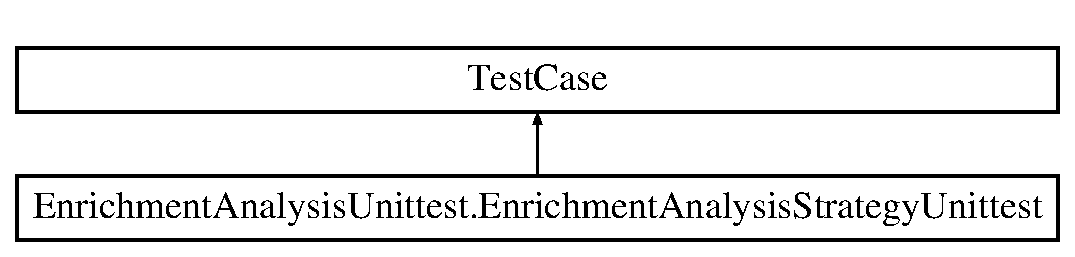
\includegraphics[height=2.000000cm]{classEnrichmentAnalysisUnittest_1_1EnrichmentAnalysisStrategyUnittest}
\end{center}
\end{figure}
\subsection*{Public Member Functions}
\begin{DoxyCompactItemize}
\item 
\hypertarget{classEnrichmentAnalysisUnittest_1_1EnrichmentAnalysisStrategyUnittest_ad28952734ad9ba9bb3297a59ff768483}{def {\bfseries set\-Up}}\label{classEnrichmentAnalysisUnittest_1_1EnrichmentAnalysisStrategyUnittest_ad28952734ad9ba9bb3297a59ff768483}

\item 
\hypertarget{classEnrichmentAnalysisUnittest_1_1EnrichmentAnalysisStrategyUnittest_acc7ca5f6a32b1a52a1e115c299a92aae}{def {\bfseries test\-\_\-default\-\_\-params}}\label{classEnrichmentAnalysisUnittest_1_1EnrichmentAnalysisStrategyUnittest_acc7ca5f6a32b1a52a1e115c299a92aae}

\item 
\hypertarget{classEnrichmentAnalysisUnittest_1_1EnrichmentAnalysisStrategyUnittest_ab1a970addff22293218c5a0e2c1b4760}{def {\bfseries test\-\_\-multiple\-\_\-correction}}\label{classEnrichmentAnalysisUnittest_1_1EnrichmentAnalysisStrategyUnittest_ab1a970addff22293218c5a0e2c1b4760}

\item 
\hypertarget{classEnrichmentAnalysisUnittest_1_1EnrichmentAnalysisStrategyUnittest_a478023f4e18773d7bfa4d23030767929}{def {\bfseries test\-\_\-count\-\_\-sign\-\_\-tests}}\label{classEnrichmentAnalysisUnittest_1_1EnrichmentAnalysisStrategyUnittest_a478023f4e18773d7bfa4d23030767929}

\item 
\hypertarget{classEnrichmentAnalysisUnittest_1_1EnrichmentAnalysisStrategyUnittest_a86faa88b85eaf81c504e06f4317f8437}{def {\bfseries test\-\_\-randomize\-\_\-proteins}}\label{classEnrichmentAnalysisUnittest_1_1EnrichmentAnalysisStrategyUnittest_a86faa88b85eaf81c504e06f4317f8437}

\item 
\hypertarget{classEnrichmentAnalysisUnittest_1_1EnrichmentAnalysisStrategyUnittest_a7b60b0a38e8b25abb0ca2d04ea48b866}{def {\bfseries test\-\_\-run\-\_\-rna\-\_\-vs\-\_\-annotations}}\label{classEnrichmentAnalysisUnittest_1_1EnrichmentAnalysisStrategyUnittest_a7b60b0a38e8b25abb0ca2d04ea48b866}

\item 
\hypertarget{classEnrichmentAnalysisUnittest_1_1EnrichmentAnalysisStrategyUnittest_a473e91253bb32ca541b7f42d60a8dd48}{def {\bfseries test\-\_\-empirical\-\_\-pvalue}}\label{classEnrichmentAnalysisUnittest_1_1EnrichmentAnalysisStrategyUnittest_a473e91253bb32ca541b7f42d60a8dd48}

\item 
\hypertarget{classEnrichmentAnalysisUnittest_1_1EnrichmentAnalysisStrategyUnittest_ac355a0cb44be5ffb032246761efc4696}{def {\bfseries test\-\_\-hypergeometric\-\_\-test}}\label{classEnrichmentAnalysisUnittest_1_1EnrichmentAnalysisStrategyUnittest_ac355a0cb44be5ffb032246761efc4696}

\item 
\hypertarget{classEnrichmentAnalysisUnittest_1_1EnrichmentAnalysisStrategyUnittest_a6b95558918c396e1b5f7f482f30c9e38}{def {\bfseries test\-\_\-get\-\_\-interaction\-\_\-data}}\label{classEnrichmentAnalysisUnittest_1_1EnrichmentAnalysisStrategyUnittest_a6b95558918c396e1b5f7f482f30c9e38}

\item 
\hypertarget{classEnrichmentAnalysisUnittest_1_1EnrichmentAnalysisStrategyUnittest_a1d73ad9f7d0998892a528587f2cad2f1}{def {\bfseries test\-\_\-annotation\-\_\-report}}\label{classEnrichmentAnalysisUnittest_1_1EnrichmentAnalysisStrategyUnittest_a1d73ad9f7d0998892a528587f2cad2f1}

\item 
\hypertarget{classEnrichmentAnalysisUnittest_1_1EnrichmentAnalysisStrategyUnittest_ababc958cbd5b61c8932ee238c6617f54}{def {\bfseries test\-\_\-results}}\label{classEnrichmentAnalysisUnittest_1_1EnrichmentAnalysisStrategyUnittest_ababc958cbd5b61c8932ee238c6617f54}

\item 
\hypertarget{classEnrichmentAnalysisUnittest_1_1EnrichmentAnalysisStrategyUnittest_a74678e1ea2ce36e69e3f33047bdc0613}{def {\bfseries test\-\_\-retrieve\-\_\-expression}}\label{classEnrichmentAnalysisUnittest_1_1EnrichmentAnalysisStrategyUnittest_a74678e1ea2ce36e69e3f33047bdc0613}

\item 
\hypertarget{classEnrichmentAnalysisUnittest_1_1EnrichmentAnalysisStrategyUnittest_a47a436f1293aed84f8f689665745d2b9}{def {\bfseries test\-\_\-expression\-\_\-warning}}\label{classEnrichmentAnalysisUnittest_1_1EnrichmentAnalysisStrategyUnittest_a47a436f1293aed84f8f689665745d2b9}

\item 
\hypertarget{classEnrichmentAnalysisUnittest_1_1EnrichmentAnalysisStrategyUnittest_a191a8ce0c525667957e8c9ba98e8d874}{def {\bfseries tear\-Down}}\label{classEnrichmentAnalysisUnittest_1_1EnrichmentAnalysisStrategyUnittest_a191a8ce0c525667957e8c9ba98e8d874}

\end{DoxyCompactItemize}
\subsection*{Public Attributes}
\begin{DoxyCompactItemize}
\item 
\hypertarget{classEnrichmentAnalysisUnittest_1_1EnrichmentAnalysisStrategyUnittest_a4645eebe2adb7fc3e5627d39f189fd53}{{\bfseries sql\-\_\-session}}\label{classEnrichmentAnalysisUnittest_1_1EnrichmentAnalysisStrategyUnittest_a4645eebe2adb7fc3e5627d39f189fd53}

\item 
\hypertarget{classEnrichmentAnalysisUnittest_1_1EnrichmentAnalysisStrategyUnittest_a28a5765ad3523027fa0a5999e3038d45}{{\bfseries expected\-Folder}}\label{classEnrichmentAnalysisUnittest_1_1EnrichmentAnalysisStrategyUnittest_a28a5765ad3523027fa0a5999e3038d45}

\item 
\hypertarget{classEnrichmentAnalysisUnittest_1_1EnrichmentAnalysisStrategyUnittest_ad181adcbad84b7fcefda7d8a52cd02a5}{{\bfseries output\-Folder}}\label{classEnrichmentAnalysisUnittest_1_1EnrichmentAnalysisStrategyUnittest_ad181adcbad84b7fcefda7d8a52cd02a5}

\item 
\hypertarget{classEnrichmentAnalysisUnittest_1_1EnrichmentAnalysisStrategyUnittest_ac69241ee8617cb4bc51818dee988d0c5}{{\bfseries run}}\label{classEnrichmentAnalysisUnittest_1_1EnrichmentAnalysisStrategyUnittest_ac69241ee8617cb4bc51818dee988d0c5}

\end{DoxyCompactItemize}
\subsection*{Static Public Attributes}
\begin{DoxyCompactItemize}
\item 
\hypertarget{classEnrichmentAnalysisUnittest_1_1EnrichmentAnalysisStrategyUnittest_aca3d4e3b0cdb3c2485cd79525310a035}{tuple {\bfseries expected\-Number\-Tests} = len( self.\-run.\-annot\-With\-Interaction\-Dict)}\label{classEnrichmentAnalysisUnittest_1_1EnrichmentAnalysisStrategyUnittest_aca3d4e3b0cdb3c2485cd79525310a035}

\item 
\hypertarget{classEnrichmentAnalysisUnittest_1_1EnrichmentAnalysisStrategyUnittest_ad54ac92c0684f061c282f65f0d32e392}{int {\bfseries count\-Lines} = 0}\label{classEnrichmentAnalysisUnittest_1_1EnrichmentAnalysisStrategyUnittest_ad54ac92c0684f061c282f65f0d32e392}

\item 
\hypertarget{classEnrichmentAnalysisUnittest_1_1EnrichmentAnalysisStrategyUnittest_a9449476f7b177676715447447f43c148}{int {\bfseries count\-Test\-Per\-R\-N\-A} = 0}\label{classEnrichmentAnalysisUnittest_1_1EnrichmentAnalysisStrategyUnittest_a9449476f7b177676715447447f43c148}

\end{DoxyCompactItemize}


The documentation for this class was generated from the following file\-:\begin{DoxyCompactItemize}
\item 
test/fr/tagc/rainet/core/execution/Enrichment\-Analysis\-Unittest.\-py\end{DoxyCompactItemize}

\hypertarget{classsrc_1_1core_1_1util_1_1databases_1_1Ensembl_1_1Ensembl}{\section{src.\-core.\-util.\-databases.\-Ensembl.\-Ensembl Class Reference}
\label{classsrc_1_1core_1_1util_1_1databases_1_1Ensembl_1_1Ensembl}\index{src.\-core.\-util.\-databases.\-Ensembl.\-Ensembl@{src.\-core.\-util.\-databases.\-Ensembl.\-Ensembl}}
}
\subsection*{Public Member Functions}
\begin{DoxyCompactItemize}
\item 
\hypertarget{classsrc_1_1core_1_1util_1_1databases_1_1Ensembl_1_1Ensembl_a1dc3d0a5667f131cd77be8bac22d4602}{def {\bfseries \-\_\-\-\_\-init\-\_\-\-\_\-}}\label{classsrc_1_1core_1_1util_1_1databases_1_1Ensembl_1_1Ensembl_a1dc3d0a5667f131cd77be8bac22d4602}

\item 
\hypertarget{classsrc_1_1core_1_1util_1_1databases_1_1Ensembl_1_1Ensembl_a81456966dbd60a73c87ffb64383571d0}{def {\bfseries connection}}\label{classsrc_1_1core_1_1util_1_1databases_1_1Ensembl_1_1Ensembl_a81456966dbd60a73c87ffb64383571d0}

\end{DoxyCompactItemize}
\subsection*{Static Public Member Functions}
\begin{DoxyCompactItemize}
\item 
\hypertarget{classsrc_1_1core_1_1util_1_1databases_1_1Ensembl_1_1Ensembl_a96b5cbb2a743faa1b7df8b14b1ce90f0}{def {\bfseries get\-\_\-sequence}}\label{classsrc_1_1core_1_1util_1_1databases_1_1Ensembl_1_1Ensembl_a96b5cbb2a743faa1b7df8b14b1ce90f0}

\item 
\hypertarget{classsrc_1_1core_1_1util_1_1databases_1_1Ensembl_1_1Ensembl_a3c15bb86cc8e1ad0f27800bc1d43c5d1}{def {\bfseries get\-\_\-header}}\label{classsrc_1_1core_1_1util_1_1databases_1_1Ensembl_1_1Ensembl_a3c15bb86cc8e1ad0f27800bc1d43c5d1}

\item 
\hypertarget{classsrc_1_1core_1_1util_1_1databases_1_1Ensembl_1_1Ensembl_a81538bec6fad9516f2739ef69568c627}{def {\bfseries list\-\_\-get\-\_\-seq}}\label{classsrc_1_1core_1_1util_1_1databases_1_1Ensembl_1_1Ensembl_a81538bec6fad9516f2739ef69568c627}

\end{DoxyCompactItemize}
\subsection*{Public Attributes}
\begin{DoxyCompactItemize}
\item 
\hypertarget{classsrc_1_1core_1_1util_1_1databases_1_1Ensembl_1_1Ensembl_a151c76933d0a67aed4cbf40de94c792e}{{\bfseries server}}\label{classsrc_1_1core_1_1util_1_1databases_1_1Ensembl_1_1Ensembl_a151c76933d0a67aed4cbf40de94c792e}

\item 
\hypertarget{classsrc_1_1core_1_1util_1_1databases_1_1Ensembl_1_1Ensembl_af4bc1c81978e0d06512fdec5330f46a2}{{\bfseries end}}\label{classsrc_1_1core_1_1util_1_1databases_1_1Ensembl_1_1Ensembl_af4bc1c81978e0d06512fdec5330f46a2}

\item 
\hypertarget{classsrc_1_1core_1_1util_1_1databases_1_1Ensembl_1_1Ensembl_ab7d59100515d2843950b7208db4a90ab}{{\bfseries dict\-\_\-query}}\label{classsrc_1_1core_1_1util_1_1databases_1_1Ensembl_1_1Ensembl_ab7d59100515d2843950b7208db4a90ab}

\item 
\hypertarget{classsrc_1_1core_1_1util_1_1databases_1_1Ensembl_1_1Ensembl_abe0848d95dc5ebd1b32cf499c5ac4bff}{{\bfseries section}}\label{classsrc_1_1core_1_1util_1_1databases_1_1Ensembl_1_1Ensembl_abe0848d95dc5ebd1b32cf499c5ac4bff}

\end{DoxyCompactItemize}


The documentation for this class was generated from the following file\-:\begin{DoxyCompactItemize}
\item 
rbp-\/motif/src/core/util/databases/Ensembl.\-py\end{DoxyCompactItemize}

\hypertarget{classsrc_1_1fr_1_1tagc_1_1rainet_1_1core_1_1execution_1_1ExecutionStrategy_1_1ExecutionStrategy}{\section{src.\-fr.\-tagc.\-rainet.\-core.\-execution.\-Execution\-Strategy.\-Execution\-Strategy Class Reference}
\label{classsrc_1_1fr_1_1tagc_1_1rainet_1_1core_1_1execution_1_1ExecutionStrategy_1_1ExecutionStrategy}\index{src.\-fr.\-tagc.\-rainet.\-core.\-execution.\-Execution\-Strategy.\-Execution\-Strategy@{src.\-fr.\-tagc.\-rainet.\-core.\-execution.\-Execution\-Strategy.\-Execution\-Strategy}}
}
Inheritance diagram for src.\-fr.\-tagc.\-rainet.\-core.\-execution.\-Execution\-Strategy.\-Execution\-Strategy\-:\begin{figure}[H]
\begin{center}
\leavevmode
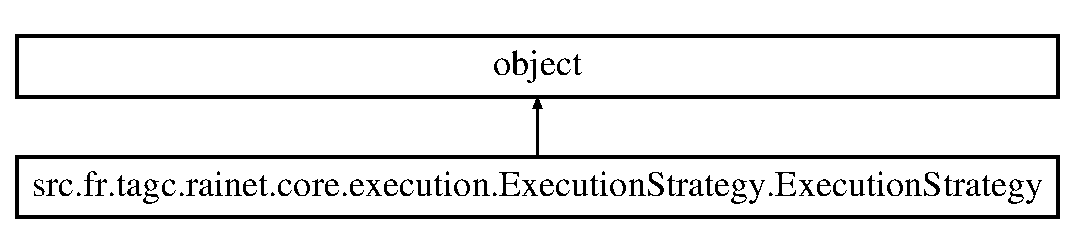
\includegraphics[height=2.000000cm]{classsrc_1_1fr_1_1tagc_1_1rainet_1_1core_1_1execution_1_1ExecutionStrategy_1_1ExecutionStrategy}
\end{center}
\end{figure}
\subsection*{Public Member Functions}
\begin{DoxyCompactItemize}
\item 
\hypertarget{classsrc_1_1fr_1_1tagc_1_1rainet_1_1core_1_1execution_1_1ExecutionStrategy_1_1ExecutionStrategy_afaf8d52a0852fc7f8aa501f376f4e5dd}{def {\bfseries execute}}\label{classsrc_1_1fr_1_1tagc_1_1rainet_1_1core_1_1execution_1_1ExecutionStrategy_1_1ExecutionStrategy_afaf8d52a0852fc7f8aa501f376f4e5dd}

\end{DoxyCompactItemize}


The documentation for this class was generated from the following file\-:\begin{DoxyCompactItemize}
\item 
src/fr/tagc/rainet/core/execution/Execution\-Strategy.\-py\end{DoxyCompactItemize}

\hypertarget{classExploreInteractingRNAs_1_1ExploreInteractingRNAs}{\section{Explore\-Interacting\-R\-N\-As.\-Explore\-Interacting\-R\-N\-As Class Reference}
\label{classExploreInteractingRNAs_1_1ExploreInteractingRNAs}\index{Explore\-Interacting\-R\-N\-As.\-Explore\-Interacting\-R\-N\-As@{Explore\-Interacting\-R\-N\-As.\-Explore\-Interacting\-R\-N\-As}}
}
Inheritance diagram for Explore\-Interacting\-R\-N\-As.\-Explore\-Interacting\-R\-N\-As\-:\begin{figure}[H]
\begin{center}
\leavevmode
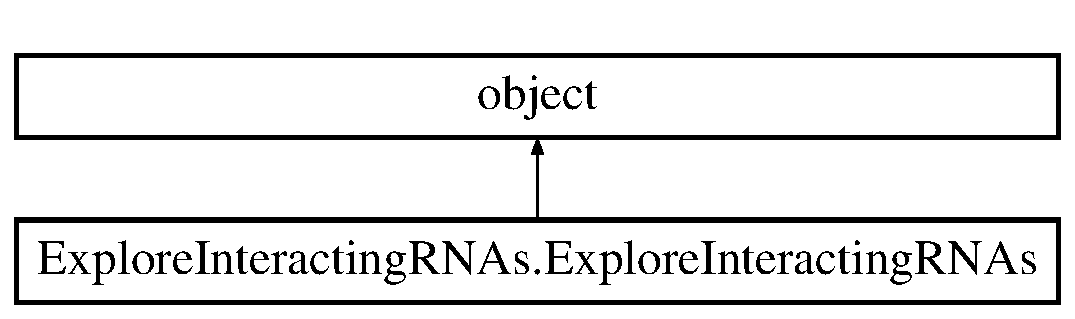
\includegraphics[height=2.000000cm]{classExploreInteractingRNAs_1_1ExploreInteractingRNAs}
\end{center}
\end{figure}
\subsection*{Public Member Functions}
\begin{DoxyCompactItemize}
\item 
\hypertarget{classExploreInteractingRNAs_1_1ExploreInteractingRNAs_a289c542fab38cbad34fc8c32dae42d8f}{def {\bfseries \-\_\-\-\_\-init\-\_\-\-\_\-}}\label{classExploreInteractingRNAs_1_1ExploreInteractingRNAs_a289c542fab38cbad34fc8c32dae42d8f}

\item 
\hypertarget{classExploreInteractingRNAs_1_1ExploreInteractingRNAs_a55c3ed4fa3a3bbb4c84c9c86e8820ec6}{def {\bfseries read\-\_\-transcript\-\_\-list}}\label{classExploreInteractingRNAs_1_1ExploreInteractingRNAs_a55c3ed4fa3a3bbb4c84c9c86e8820ec6}

\item 
\hypertarget{classExploreInteractingRNAs_1_1ExploreInteractingRNAs_a5d43c036316bfb393b5a7d828239ef50}{def {\bfseries query\-\_\-database}}\label{classExploreInteractingRNAs_1_1ExploreInteractingRNAs_a5d43c036316bfb393b5a7d828239ef50}

\end{DoxyCompactItemize}
\subsection*{Public Attributes}
\begin{DoxyCompactItemize}
\item 
\hypertarget{classExploreInteractingRNAs_1_1ExploreInteractingRNAs_a9766a57b46e4c757fea56d982dcf4c1d}{{\bfseries rainet\-D\-B}}\label{classExploreInteractingRNAs_1_1ExploreInteractingRNAs_a9766a57b46e4c757fea56d982dcf4c1d}

\item 
\hypertarget{classExploreInteractingRNAs_1_1ExploreInteractingRNAs_a44e475ab1d8de56637448d5e97ce2001}{{\bfseries transcript\-List}}\label{classExploreInteractingRNAs_1_1ExploreInteractingRNAs_a44e475ab1d8de56637448d5e97ce2001}

\item 
\hypertarget{classExploreInteractingRNAs_1_1ExploreInteractingRNAs_a6c783199f4b5ad292531b5cc906444d6}{{\bfseries interacting\-Transcript\-List}}\label{classExploreInteractingRNAs_1_1ExploreInteractingRNAs_a6c783199f4b5ad292531b5cc906444d6}

\item 
\hypertarget{classExploreInteractingRNAs_1_1ExploreInteractingRNAs_afb54fb60daa74e958ada65c925a5c416}{{\bfseries output\-Folder}}\label{classExploreInteractingRNAs_1_1ExploreInteractingRNAs_afb54fb60daa74e958ada65c925a5c416}

\item 
\hypertarget{classExploreInteractingRNAs_1_1ExploreInteractingRNAs_a7c2ff7ec8203c24467db6b0ad66578ed}{{\bfseries sql\-\_\-session}}\label{classExploreInteractingRNAs_1_1ExploreInteractingRNAs_a7c2ff7ec8203c24467db6b0ad66578ed}

\end{DoxyCompactItemize}
\subsection*{Static Public Attributes}
\begin{DoxyCompactItemize}
\item 
\hypertarget{classExploreInteractingRNAs_1_1ExploreInteractingRNAs_a06a679952025f5a49ae1cbed1f407471}{string {\bfseries R\-N\-A\-\_\-\-A\-L\-L\-\_\-\-K\-W} = \char`\"{}all\-R\-N\-As\char`\"{}}\label{classExploreInteractingRNAs_1_1ExploreInteractingRNAs_a06a679952025f5a49ae1cbed1f407471}

\end{DoxyCompactItemize}


The documentation for this class was generated from the following file\-:\begin{DoxyCompactItemize}
\item 
src/fr/tagc/rainet/core/execution/processing/known\-Scaffold\-Examples/Explore\-Interacting\-R\-N\-As.\-py\end{DoxyCompactItemize}

\hypertarget{classsrc_1_1fr_1_1tagc_1_1rainet_1_1core_1_1util_1_1parser_1_1FastaParser_1_1FastaParser}{\section{src.\-fr.\-tagc.\-rainet.\-core.\-util.\-parser.\-Fasta\-Parser.\-Fasta\-Parser Class Reference}
\label{classsrc_1_1fr_1_1tagc_1_1rainet_1_1core_1_1util_1_1parser_1_1FastaParser_1_1FastaParser}\index{src.\-fr.\-tagc.\-rainet.\-core.\-util.\-parser.\-Fasta\-Parser.\-Fasta\-Parser@{src.\-fr.\-tagc.\-rainet.\-core.\-util.\-parser.\-Fasta\-Parser.\-Fasta\-Parser}}
}


This class is a parser of tab separated text file.  


Inheritance diagram for src.\-fr.\-tagc.\-rainet.\-core.\-util.\-parser.\-Fasta\-Parser.\-Fasta\-Parser\-:\begin{figure}[H]
\begin{center}
\leavevmode
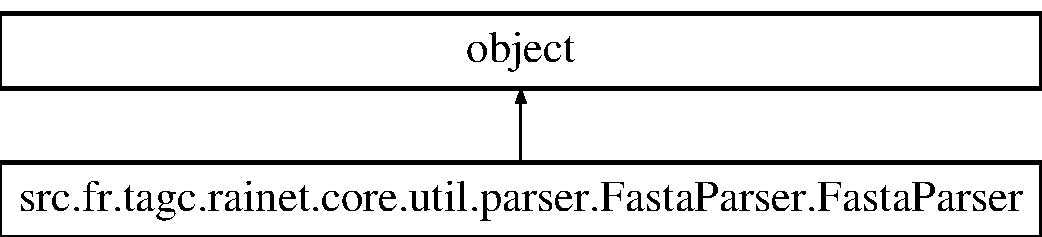
\includegraphics[height=2.000000cm]{classsrc_1_1fr_1_1tagc_1_1rainet_1_1core_1_1util_1_1parser_1_1FastaParser_1_1FastaParser}
\end{center}
\end{figure}
\subsection*{Static Public Member Functions}
\begin{DoxyCompactItemize}
\item 
def \hyperlink{classsrc_1_1fr_1_1tagc_1_1rainet_1_1core_1_1util_1_1parser_1_1FastaParser_1_1FastaParser_aa8e952bd3fba70c0f1e6936f72a30bc2}{parse\-\_\-file}
\begin{DoxyCompactList}\small\item\em This method parses the provided T\-S\-V file, looking for headers if required and creating one Object of the requested Class per line. \end{DoxyCompactList}\end{DoxyCompactItemize}


\subsection{Detailed Description}
This class is a parser of tab separated text file. 

The class contains methods allowing to parse any T\-S\-V file by creating a specific type of Object for each line found The parser have to received as input\-:
\begin{DoxyItemize}
\item The path to the file to parse
\item The information on the presence or not of column headers in the file
\item The ordered list of column headers (if headers are not present or if user want to overwrite file header values)
\item The name of the Class corresponding to Object to be created for each file line
\item The ordered list of header names to use to call the Class constructor
\item The ordered list of optional values to use to call the Class constructor
\item The comment symbol
\item The information indicating if the related db table must be cleaned before insertion or not 
\end{DoxyItemize}

\subsection{Member Function Documentation}
\hypertarget{classsrc_1_1fr_1_1tagc_1_1rainet_1_1core_1_1util_1_1parser_1_1FastaParser_1_1FastaParser_aa8e952bd3fba70c0f1e6936f72a30bc2}{\index{src\-::fr\-::tagc\-::rainet\-::core\-::util\-::parser\-::\-Fasta\-Parser\-::\-Fasta\-Parser@{src\-::fr\-::tagc\-::rainet\-::core\-::util\-::parser\-::\-Fasta\-Parser\-::\-Fasta\-Parser}!parse\-\_\-file@{parse\-\_\-file}}
\index{parse\-\_\-file@{parse\-\_\-file}!src::fr::tagc::rainet::core::util::parser::FastaParser::FastaParser@{src\-::fr\-::tagc\-::rainet\-::core\-::util\-::parser\-::\-Fasta\-Parser\-::\-Fasta\-Parser}}
\subsubsection[{parse\-\_\-file}]{\setlength{\rightskip}{0pt plus 5cm}def src.\-fr.\-tagc.\-rainet.\-core.\-util.\-parser.\-Fasta\-Parser.\-Fasta\-Parser.\-parse\-\_\-file (
\begin{DoxyParamCaption}
\item[{}]{file\-\_\-path, }
\item[{}]{class\-\_\-name, }
\item[{}]{regular\-\_\-expression, }
\item[{}]{group\-\_\-list, }
\item[{}]{parameter\-\_\-name\-\_\-list, }
\item[{}]{parameter\-\_\-value\-\_\-list, }
\item[{}]{comment\-\_\-symbol, }
\item[{}]{clean\-\_\-table = {\ttfamily True}}
\end{DoxyParamCaption}
)\hspace{0.3cm}{\ttfamily [static]}}}\label{classsrc_1_1fr_1_1tagc_1_1rainet_1_1core_1_1util_1_1parser_1_1FastaParser_1_1FastaParser_aa8e952bd3fba70c0f1e6936f72a30bc2}


This method parses the provided T\-S\-V file, looking for headers if required and creating one Object of the requested Class per line. 


\begin{DoxyParams}{Parameters}
{\em file\-\_\-path} & \-: string -\/ The path to the T\-S\-V file to parse \\
\hline
{\em regular\-\_\-expression} & \-: string -\/ The regular expression that must match the sequence definition line \\
\hline
{\em class\-\_\-name} & \-: string -\/ name of the class to instantiate \\
\hline
{\em parameter\-\_\-name\-\_\-list} & \-: list$<$string$>$ -\/ Ordered list of parameters used to instantiate the Class \\
\hline
{\em parameter\-\_\-value\-\_\-list} & \-: list$<$string$>$ -\/ Ordered list of optional parameter values used to instantiate the Class \\
\hline
{\em comment\-\_\-symbol} & \-: string -\/ symbol used to comment lines in the file to parse \\
\hline
{\em clean\-\_\-table} & \-: boolean -\/ The information indicating if the related db table must be cleaned before insertion or not\\
\hline
\end{DoxyParams}
\begin{DoxyReturn}{Returns}
None 
\end{DoxyReturn}


The documentation for this class was generated from the following file\-:\begin{DoxyCompactItemize}
\item 
src/fr/tagc/rainet/core/util/parser/Fasta\-Parser.\-py\end{DoxyCompactItemize}

\hypertarget{classsrc_1_1core_1_1util_1_1exception_1_1FileFormatException_1_1FileFormatException}{\section{src.\-core.\-util.\-exception.\-File\-Format\-Exception.\-File\-Format\-Exception Class Reference}
\label{classsrc_1_1core_1_1util_1_1exception_1_1FileFormatException_1_1FileFormatException}\index{src.\-core.\-util.\-exception.\-File\-Format\-Exception.\-File\-Format\-Exception@{src.\-core.\-util.\-exception.\-File\-Format\-Exception.\-File\-Format\-Exception}}
}


Exception raised in case of file format given in a method is not appropriated.  


\subsection*{Public Member Functions}
\begin{DoxyCompactItemize}
\item 
\hypertarget{classsrc_1_1core_1_1util_1_1exception_1_1FileFormatException_1_1FileFormatException_a5cbad1b7a1ccf70256a3d18949ed2193}{def {\bfseries \-\_\-\-\_\-init\-\_\-\-\_\-}}\label{classsrc_1_1core_1_1util_1_1exception_1_1FileFormatException_1_1FileFormatException_a5cbad1b7a1ccf70256a3d18949ed2193}

\item 
\hypertarget{classsrc_1_1core_1_1util_1_1exception_1_1FileFormatException_1_1FileFormatException_a6601baad957387006ac24b21d02e8730}{def {\bfseries print\-\_\-error}}\label{classsrc_1_1core_1_1util_1_1exception_1_1FileFormatException_1_1FileFormatException_a6601baad957387006ac24b21d02e8730}

\end{DoxyCompactItemize}
\subsection*{Public Attributes}
\begin{DoxyCompactItemize}
\item 
\hypertarget{classsrc_1_1core_1_1util_1_1exception_1_1FileFormatException_1_1FileFormatException_a947a4fc6c58e82e619ab3a9c7e85a2e4}{{\bfseries message}}\label{classsrc_1_1core_1_1util_1_1exception_1_1FileFormatException_1_1FileFormatException_a947a4fc6c58e82e619ab3a9c7e85a2e4}

\end{DoxyCompactItemize}


\subsection{Detailed Description}
Exception raised in case of file format given in a method is not appropriated. 

The documentation for this class was generated from the following file\-:\begin{DoxyCompactItemize}
\item 
rbp-\/motif/src/core/util/exception/File\-Format\-Exception.\-py\end{DoxyCompactItemize}

\hypertarget{classsrc_1_1fr_1_1tagc_1_1rainet_1_1core_1_1util_1_1exception_1_1FileFormatException_1_1FileFormatException}{\section{src.\-fr.\-tagc.\-rainet.\-core.\-util.\-exception.\-File\-Format\-Exception.\-File\-Format\-Exception Class Reference}
\label{classsrc_1_1fr_1_1tagc_1_1rainet_1_1core_1_1util_1_1exception_1_1FileFormatException_1_1FileFormatException}\index{src.\-fr.\-tagc.\-rainet.\-core.\-util.\-exception.\-File\-Format\-Exception.\-File\-Format\-Exception@{src.\-fr.\-tagc.\-rainet.\-core.\-util.\-exception.\-File\-Format\-Exception.\-File\-Format\-Exception}}
}


Exception raised in case of file format given in a method is not appropriated.  


Inheritance diagram for src.\-fr.\-tagc.\-rainet.\-core.\-util.\-exception.\-File\-Format\-Exception.\-File\-Format\-Exception\-:\begin{figure}[H]
\begin{center}
\leavevmode
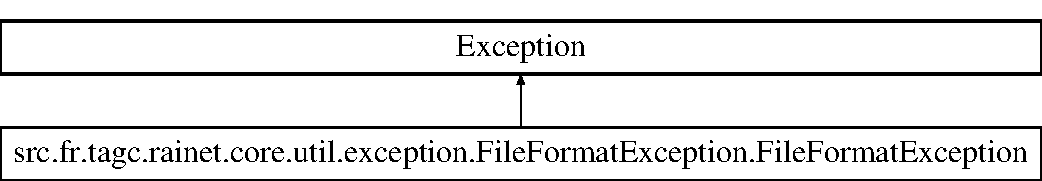
\includegraphics[height=2.000000cm]{classsrc_1_1fr_1_1tagc_1_1rainet_1_1core_1_1util_1_1exception_1_1FileFormatException_1_1FileFormatException}
\end{center}
\end{figure}
\subsection*{Public Member Functions}
\begin{DoxyCompactItemize}
\item 
\hypertarget{classsrc_1_1fr_1_1tagc_1_1rainet_1_1core_1_1util_1_1exception_1_1FileFormatException_1_1FileFormatException_abb3c1d106d1f5434869e7aad4a18aff0}{def {\bfseries \-\_\-\-\_\-init\-\_\-\-\_\-}}\label{classsrc_1_1fr_1_1tagc_1_1rainet_1_1core_1_1util_1_1exception_1_1FileFormatException_1_1FileFormatException_abb3c1d106d1f5434869e7aad4a18aff0}

\item 
\hypertarget{classsrc_1_1fr_1_1tagc_1_1rainet_1_1core_1_1util_1_1exception_1_1FileFormatException_1_1FileFormatException_a32abe45d4867ca201346d1dd3a4e69ba}{def {\bfseries print\-\_\-error}}\label{classsrc_1_1fr_1_1tagc_1_1rainet_1_1core_1_1util_1_1exception_1_1FileFormatException_1_1FileFormatException_a32abe45d4867ca201346d1dd3a4e69ba}

\end{DoxyCompactItemize}
\subsection*{Public Attributes}
\begin{DoxyCompactItemize}
\item 
\hypertarget{classsrc_1_1fr_1_1tagc_1_1rainet_1_1core_1_1util_1_1exception_1_1FileFormatException_1_1FileFormatException_aa199dfd8c7e58f6832074ee235628f21}{{\bfseries message}}\label{classsrc_1_1fr_1_1tagc_1_1rainet_1_1core_1_1util_1_1exception_1_1FileFormatException_1_1FileFormatException_aa199dfd8c7e58f6832074ee235628f21}

\end{DoxyCompactItemize}


\subsection{Detailed Description}
Exception raised in case of file format given in a method is not appropriated. 

The documentation for this class was generated from the following file\-:\begin{DoxyCompactItemize}
\item 
src/fr/tagc/rainet/core/util/exception/File\-Format\-Exception.\-py\end{DoxyCompactItemize}

\hypertarget{classsrc_1_1core_1_1util_1_1parsing_1_1FileParser_1_1FileParser}{\section{src.\-core.\-util.\-parsing.\-File\-Parser.\-File\-Parser Class Reference}
\label{classsrc_1_1core_1_1util_1_1parsing_1_1FileParser_1_1FileParser}\index{src.\-core.\-util.\-parsing.\-File\-Parser.\-File\-Parser@{src.\-core.\-util.\-parsing.\-File\-Parser.\-File\-Parser}}
}
\subsection*{Static Public Member Functions}
\begin{DoxyCompactItemize}
\item 
\hypertarget{classsrc_1_1core_1_1util_1_1parsing_1_1FileParser_1_1FileParser_a083431cc05609eaeb06884c263e52438}{def {\bfseries read\-\_\-file}}\label{classsrc_1_1core_1_1util_1_1parsing_1_1FileParser_1_1FileParser_a083431cc05609eaeb06884c263e52438}

\item 
\hypertarget{classsrc_1_1core_1_1util_1_1parsing_1_1FileParser_1_1FileParser_ab260d5d8898863708d94c8c8cfad23f7}{def {\bfseries make\-\_\-table}}\label{classsrc_1_1core_1_1util_1_1parsing_1_1FileParser_1_1FileParser_ab260d5d8898863708d94c8c8cfad23f7}

\item 
\hypertarget{classsrc_1_1core_1_1util_1_1parsing_1_1FileParser_1_1FileParser_aee319cc277e01692cc6095180021ab1b}{def {\bfseries merge\-\_\-file}}\label{classsrc_1_1core_1_1util_1_1parsing_1_1FileParser_1_1FileParser_aee319cc277e01692cc6095180021ab1b}

\end{DoxyCompactItemize}


The documentation for this class was generated from the following file\-:\begin{DoxyCompactItemize}
\item 
rbp-\/motif/src/core/util/parsing/File\-Parser.\-py\end{DoxyCompactItemize}

\hypertarget{classsrc_1_1core_1_1util_1_1file_1_1FileUtils_1_1FileUtils}{\section{src.\-core.\-util.\-file.\-File\-Utils.\-File\-Utils Class Reference}
\label{classsrc_1_1core_1_1util_1_1file_1_1FileUtils_1_1FileUtils}\index{src.\-core.\-util.\-file.\-File\-Utils.\-File\-Utils@{src.\-core.\-util.\-file.\-File\-Utils.\-File\-Utils}}
}


This class contains static methods that are used to manipulate files like open  and close, but some others like find extension.  


Inheritance diagram for src.\-core.\-util.\-file.\-File\-Utils.\-File\-Utils\-:\begin{figure}[H]
\begin{center}
\leavevmode
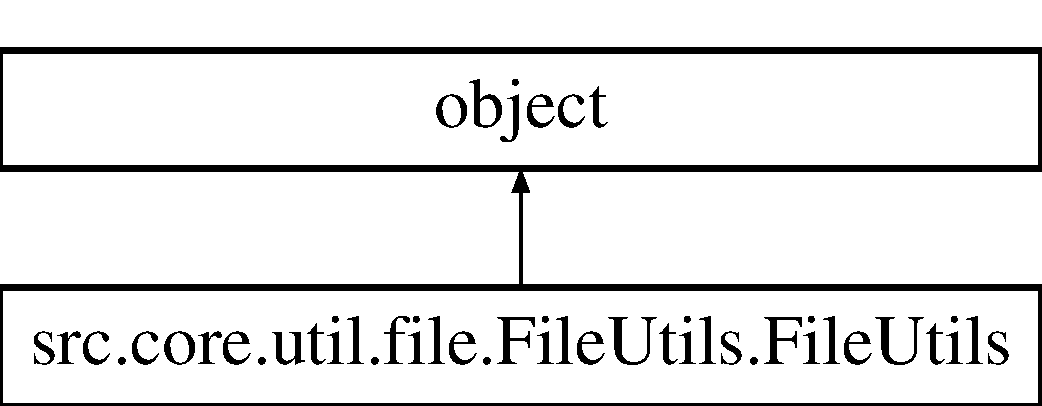
\includegraphics[height=2.000000cm]{classsrc_1_1core_1_1util_1_1file_1_1FileUtils_1_1FileUtils}
\end{center}
\end{figure}
\subsection*{Static Public Member Functions}
\begin{DoxyCompactItemize}
\item 
\hypertarget{classsrc_1_1core_1_1util_1_1file_1_1FileUtils_1_1FileUtils_a54f1194f71a93143ed90d81a641058a0}{def {\bfseries open\-\_\-text\-\_\-r}}\label{classsrc_1_1core_1_1util_1_1file_1_1FileUtils_1_1FileUtils_a54f1194f71a93143ed90d81a641058a0}

\item 
\hypertarget{classsrc_1_1core_1_1util_1_1file_1_1FileUtils_1_1FileUtils_a79fb7777b4380b9e5fb2c91faac3541f}{def {\bfseries open\-\_\-text\-\_\-w}}\label{classsrc_1_1core_1_1util_1_1file_1_1FileUtils_1_1FileUtils_a79fb7777b4380b9e5fb2c91faac3541f}

\item 
\hypertarget{classsrc_1_1core_1_1util_1_1file_1_1FileUtils_1_1FileUtils_ab64fa0912d4073305a9cb9f0008c8eeb}{def {\bfseries open\-\_\-text\-\_\-a}}\label{classsrc_1_1core_1_1util_1_1file_1_1FileUtils_1_1FileUtils_ab64fa0912d4073305a9cb9f0008c8eeb}

\item 
\hypertarget{classsrc_1_1core_1_1util_1_1file_1_1FileUtils_1_1FileUtils_ab4909a2862c63965df1151a82537bc59}{def {\bfseries check\-\_\-extension}}\label{classsrc_1_1core_1_1util_1_1file_1_1FileUtils_1_1FileUtils_ab4909a2862c63965df1151a82537bc59}

\end{DoxyCompactItemize}


\subsection{Detailed Description}
This class contains static methods that are used to manipulate files like open  and close, but some others like find extension. 

  

The documentation for this class was generated from the following file\-:\begin{DoxyCompactItemize}
\item 
rbp-\/motif/src/core/util/file/File\-Utils.\-py\end{DoxyCompactItemize}

\hypertarget{classsrc_1_1fr_1_1tagc_1_1rainet_1_1core_1_1util_1_1file_1_1FileUtils_1_1FileUtils}{\section{src.\-fr.\-tagc.\-rainet.\-core.\-util.\-file.\-File\-Utils.\-File\-Utils Class Reference}
\label{classsrc_1_1fr_1_1tagc_1_1rainet_1_1core_1_1util_1_1file_1_1FileUtils_1_1FileUtils}\index{src.\-fr.\-tagc.\-rainet.\-core.\-util.\-file.\-File\-Utils.\-File\-Utils@{src.\-fr.\-tagc.\-rainet.\-core.\-util.\-file.\-File\-Utils.\-File\-Utils}}
}


This class contains static methods that are used to manipulate files like open  and close, but some others like find extension.  


Inheritance diagram for src.\-fr.\-tagc.\-rainet.\-core.\-util.\-file.\-File\-Utils.\-File\-Utils\-:\begin{figure}[H]
\begin{center}
\leavevmode
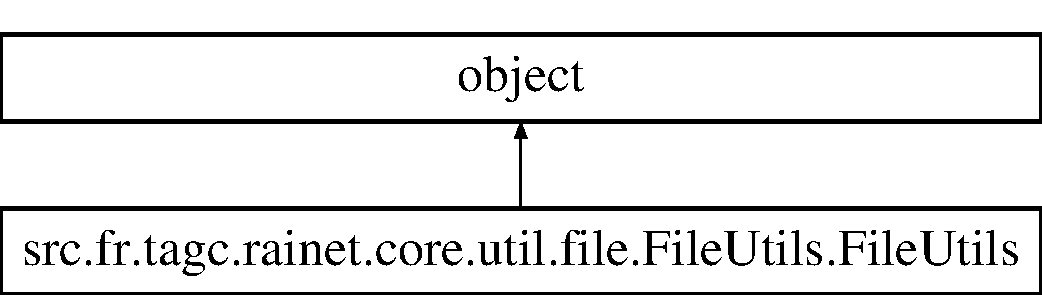
\includegraphics[height=2.000000cm]{classsrc_1_1fr_1_1tagc_1_1rainet_1_1core_1_1util_1_1file_1_1FileUtils_1_1FileUtils}
\end{center}
\end{figure}
\subsection*{Static Public Member Functions}
\begin{DoxyCompactItemize}
\item 
def \hyperlink{classsrc_1_1fr_1_1tagc_1_1rainet_1_1core_1_1util_1_1file_1_1FileUtils_1_1FileUtils_acfc8804244b1c549456d8c000b23163d}{initialise\-\_\-output\-\_\-folders}
\begin{DoxyCompactList}\small\item\em \subsubsection*{initialise\-\_\-output\-\_\-folder }\end{DoxyCompactList}\item 
\hypertarget{classsrc_1_1fr_1_1tagc_1_1rainet_1_1core_1_1util_1_1file_1_1FileUtils_1_1FileUtils_acd192c7ce19c8e57ed735f73f5fbbc07}{def {\bfseries open\-\_\-text\-\_\-r}}\label{classsrc_1_1fr_1_1tagc_1_1rainet_1_1core_1_1util_1_1file_1_1FileUtils_1_1FileUtils_acd192c7ce19c8e57ed735f73f5fbbc07}

\item 
\hypertarget{classsrc_1_1fr_1_1tagc_1_1rainet_1_1core_1_1util_1_1file_1_1FileUtils_1_1FileUtils_acf2cc959f240addda567709e355594e2}{def {\bfseries open\-\_\-text\-\_\-w}}\label{classsrc_1_1fr_1_1tagc_1_1rainet_1_1core_1_1util_1_1file_1_1FileUtils_1_1FileUtils_acf2cc959f240addda567709e355594e2}

\item 
\hypertarget{classsrc_1_1fr_1_1tagc_1_1rainet_1_1core_1_1util_1_1file_1_1FileUtils_1_1FileUtils_a9b4c9a8d1b47ae2b143a62b81e97fa2b}{def {\bfseries check\-\_\-extension}}\label{classsrc_1_1fr_1_1tagc_1_1rainet_1_1core_1_1util_1_1file_1_1FileUtils_1_1FileUtils_a9b4c9a8d1b47ae2b143a62b81e97fa2b}

\item 
def \hyperlink{classsrc_1_1fr_1_1tagc_1_1rainet_1_1core_1_1util_1_1file_1_1FileUtils_1_1FileUtils_a91725c6617f746588f494634873d65da}{remove\-\_\-extension}
\begin{DoxyCompactList}\small\item\em Remove the file extension from the file name if it exists. \end{DoxyCompactList}\end{DoxyCompactItemize}


\subsection{Detailed Description}
This class contains static methods that are used to manipulate files like open  and close, but some others like find extension. 

  

\subsection{Member Function Documentation}
\hypertarget{classsrc_1_1fr_1_1tagc_1_1rainet_1_1core_1_1util_1_1file_1_1FileUtils_1_1FileUtils_acfc8804244b1c549456d8c000b23163d}{\index{src\-::fr\-::tagc\-::rainet\-::core\-::util\-::file\-::\-File\-Utils\-::\-File\-Utils@{src\-::fr\-::tagc\-::rainet\-::core\-::util\-::file\-::\-File\-Utils\-::\-File\-Utils}!initialise\-\_\-output\-\_\-folders@{initialise\-\_\-output\-\_\-folders}}
\index{initialise\-\_\-output\-\_\-folders@{initialise\-\_\-output\-\_\-folders}!src::fr::tagc::rainet::core::util::file::FileUtils::FileUtils@{src\-::fr\-::tagc\-::rainet\-::core\-::util\-::file\-::\-File\-Utils\-::\-File\-Utils}}
\subsubsection[{initialise\-\_\-output\-\_\-folders}]{\setlength{\rightskip}{0pt plus 5cm}def src.\-fr.\-tagc.\-rainet.\-core.\-util.\-file.\-File\-Utils.\-File\-Utils.\-initialise\-\_\-output\-\_\-folders (
\begin{DoxyParamCaption}
\item[{}]{base\-\_\-folder}
\end{DoxyParamCaption}
)\hspace{0.3cm}{\ttfamily [static]}}}\label{classsrc_1_1fr_1_1tagc_1_1rainet_1_1core_1_1util_1_1file_1_1FileUtils_1_1FileUtils_acfc8804244b1c549456d8c000b23163d}


\subsubsection*{initialise\-\_\-output\-\_\-folder }

Initialise all Analysis output folders

Return nothing \hypertarget{classsrc_1_1fr_1_1tagc_1_1rainet_1_1core_1_1util_1_1file_1_1FileUtils_1_1FileUtils_a91725c6617f746588f494634873d65da}{\index{src\-::fr\-::tagc\-::rainet\-::core\-::util\-::file\-::\-File\-Utils\-::\-File\-Utils@{src\-::fr\-::tagc\-::rainet\-::core\-::util\-::file\-::\-File\-Utils\-::\-File\-Utils}!remove\-\_\-extension@{remove\-\_\-extension}}
\index{remove\-\_\-extension@{remove\-\_\-extension}!src::fr::tagc::rainet::core::util::file::FileUtils::FileUtils@{src\-::fr\-::tagc\-::rainet\-::core\-::util\-::file\-::\-File\-Utils\-::\-File\-Utils}}
\subsubsection[{remove\-\_\-extension}]{\setlength{\rightskip}{0pt plus 5cm}def src.\-fr.\-tagc.\-rainet.\-core.\-util.\-file.\-File\-Utils.\-File\-Utils.\-remove\-\_\-extension (
\begin{DoxyParamCaption}
\item[{}]{file\-\_\-name}
\end{DoxyParamCaption}
)\hspace{0.3cm}{\ttfamily [static]}}}\label{classsrc_1_1fr_1_1tagc_1_1rainet_1_1core_1_1util_1_1file_1_1FileUtils_1_1FileUtils_a91725c6617f746588f494634873d65da}


Remove the file extension from the file name if it exists. 


\begin{DoxyParams}{Parameters}
{\em file\-\_\-name} & \-: string -\/ the file name or file path\\
\hline
\end{DoxyParams}
\begin{DoxyReturn}{Returns}
the file\-\_\-name without the file extension 
\end{DoxyReturn}


The documentation for this class was generated from the following file\-:\begin{DoxyCompactItemize}
\item 
src/fr/tagc/rainet/core/util/file/File\-Utils.\-py\end{DoxyCompactItemize}

\hypertarget{classsrc_1_1core_1_1util_1_1file_1_1FileWriter_1_1FileWriter}{\section{src.\-core.\-util.\-file.\-File\-Writer.\-File\-Writer Class Reference}
\label{classsrc_1_1core_1_1util_1_1file_1_1FileWriter_1_1FileWriter}\index{src.\-core.\-util.\-file.\-File\-Writer.\-File\-Writer@{src.\-core.\-util.\-file.\-File\-Writer.\-File\-Writer}}
}
\subsection*{Static Public Member Functions}
\begin{DoxyCompactItemize}
\item 
\hypertarget{classsrc_1_1core_1_1util_1_1file_1_1FileWriter_1_1FileWriter_a9c4671980fd495b37bc1efdb9af1876c}{def {\bfseries write\-\_\-table}}\label{classsrc_1_1core_1_1util_1_1file_1_1FileWriter_1_1FileWriter_a9c4671980fd495b37bc1efdb9af1876c}

\end{DoxyCompactItemize}


The documentation for this class was generated from the following file\-:\begin{DoxyCompactItemize}
\item 
rbp-\/motif/src/core/util/file/File\-Writer.\-py\end{DoxyCompactItemize}

\hypertarget{classsrc_1_1fr_1_1tagc_1_1rainet_1_1core_1_1execution_1_1analysis_1_1EnrichmentAnalysis_1_1Filte941a9d7a59dd1ff35f69bc40c53c882a}{\section{src.\-fr.\-tagc.\-rainet.\-core.\-execution.\-analysis.\-Enrichment\-Analysis.\-Filter\-Enrichment\-Results.\-Filter\-Enrichment\-Results Class Reference}
\label{classsrc_1_1fr_1_1tagc_1_1rainet_1_1core_1_1execution_1_1analysis_1_1EnrichmentAnalysis_1_1Filte941a9d7a59dd1ff35f69bc40c53c882a}\index{src.\-fr.\-tagc.\-rainet.\-core.\-execution.\-analysis.\-Enrichment\-Analysis.\-Filter\-Enrichment\-Results.\-Filter\-Enrichment\-Results@{src.\-fr.\-tagc.\-rainet.\-core.\-execution.\-analysis.\-Enrichment\-Analysis.\-Filter\-Enrichment\-Results.\-Filter\-Enrichment\-Results}}
}
Inheritance diagram for src.\-fr.\-tagc.\-rainet.\-core.\-execution.\-analysis.\-Enrichment\-Analysis.\-Filter\-Enrichment\-Results.\-Filter\-Enrichment\-Results\-:\begin{figure}[H]
\begin{center}
\leavevmode
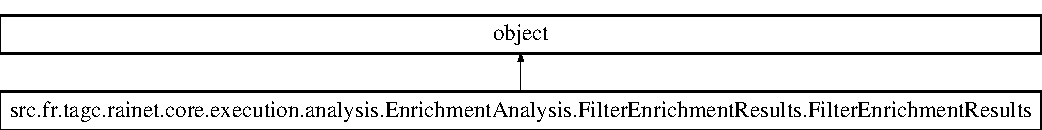
\includegraphics[height=1.750000cm]{classsrc_1_1fr_1_1tagc_1_1rainet_1_1core_1_1execution_1_1analysis_1_1EnrichmentAnalysis_1_1Filte941a9d7a59dd1ff35f69bc40c53c882a}
\end{center}
\end{figure}
\subsection*{Public Member Functions}
\begin{DoxyCompactItemize}
\item 
\hypertarget{classsrc_1_1fr_1_1tagc_1_1rainet_1_1core_1_1execution_1_1analysis_1_1EnrichmentAnalysis_1_1Filte941a9d7a59dd1ff35f69bc40c53c882a_a4afa1360cb3bd98ab2e885de0c7786a1}{def {\bfseries \-\_\-\-\_\-init\-\_\-\-\_\-}}\label{classsrc_1_1fr_1_1tagc_1_1rainet_1_1core_1_1execution_1_1analysis_1_1EnrichmentAnalysis_1_1Filte941a9d7a59dd1ff35f69bc40c53c882a_a4afa1360cb3bd98ab2e885de0c7786a1}

\item 
\hypertarget{classsrc_1_1fr_1_1tagc_1_1rainet_1_1core_1_1execution_1_1analysis_1_1EnrichmentAnalysis_1_1Filte941a9d7a59dd1ff35f69bc40c53c882a_a2bffb6ad30a5d835ea55ab449b35ff94}{def {\bfseries read\-\_\-enrichment\-\_\-per\-\_\-rna\-\_\-file}}\label{classsrc_1_1fr_1_1tagc_1_1rainet_1_1core_1_1execution_1_1analysis_1_1EnrichmentAnalysis_1_1Filte941a9d7a59dd1ff35f69bc40c53c882a_a2bffb6ad30a5d835ea55ab449b35ff94}

\item 
\hypertarget{classsrc_1_1fr_1_1tagc_1_1rainet_1_1core_1_1execution_1_1analysis_1_1EnrichmentAnalysis_1_1Filte941a9d7a59dd1ff35f69bc40c53c882a_a02c715c2dd136671cc36b879659c60ed}{def {\bfseries read\-\_\-enrichment\-\_\-results\-\_\-file}}\label{classsrc_1_1fr_1_1tagc_1_1rainet_1_1core_1_1execution_1_1analysis_1_1EnrichmentAnalysis_1_1Filte941a9d7a59dd1ff35f69bc40c53c882a_a02c715c2dd136671cc36b879659c60ed}

\item 
\hypertarget{classsrc_1_1fr_1_1tagc_1_1rainet_1_1core_1_1execution_1_1analysis_1_1EnrichmentAnalysis_1_1Filte941a9d7a59dd1ff35f69bc40c53c882a_a653b4b60426bc940f57a976d8ceb5b8d}{def {\bfseries rank\-\_\-by\-\_\-specificity}}\label{classsrc_1_1fr_1_1tagc_1_1rainet_1_1core_1_1execution_1_1analysis_1_1EnrichmentAnalysis_1_1Filte941a9d7a59dd1ff35f69bc40c53c882a_a653b4b60426bc940f57a976d8ceb5b8d}

\item 
\hypertarget{classsrc_1_1fr_1_1tagc_1_1rainet_1_1core_1_1execution_1_1analysis_1_1EnrichmentAnalysis_1_1Filte941a9d7a59dd1ff35f69bc40c53c882a_aa924cd05669e09aebe7485c9a84cadbf}{def {\bfseries read\-\_\-annotation\-\_\-file}}\label{classsrc_1_1fr_1_1tagc_1_1rainet_1_1core_1_1execution_1_1analysis_1_1EnrichmentAnalysis_1_1Filte941a9d7a59dd1ff35f69bc40c53c882a_aa924cd05669e09aebe7485c9a84cadbf}

\item 
\hypertarget{classsrc_1_1fr_1_1tagc_1_1rainet_1_1core_1_1execution_1_1analysis_1_1EnrichmentAnalysis_1_1Filte941a9d7a59dd1ff35f69bc40c53c882a_ad4db3ac5a22fbfa9a9ea2381cdc074c4}{def {\bfseries filter\-\_\-by\-\_\-specificity}}\label{classsrc_1_1fr_1_1tagc_1_1rainet_1_1core_1_1execution_1_1analysis_1_1EnrichmentAnalysis_1_1Filte941a9d7a59dd1ff35f69bc40c53c882a_ad4db3ac5a22fbfa9a9ea2381cdc074c4}

\item 
\hypertarget{classsrc_1_1fr_1_1tagc_1_1rainet_1_1core_1_1execution_1_1analysis_1_1EnrichmentAnalysis_1_1Filte941a9d7a59dd1ff35f69bc40c53c882a_a03e2e7d72268b5064c39970c93654b8d}{def {\bfseries filter\-\_\-by\-\_\-observed\-\_\-interactions}}\label{classsrc_1_1fr_1_1tagc_1_1rainet_1_1core_1_1execution_1_1analysis_1_1EnrichmentAnalysis_1_1Filte941a9d7a59dd1ff35f69bc40c53c882a_a03e2e7d72268b5064c39970c93654b8d}

\item 
\hypertarget{classsrc_1_1fr_1_1tagc_1_1rainet_1_1core_1_1execution_1_1analysis_1_1EnrichmentAnalysis_1_1Filte941a9d7a59dd1ff35f69bc40c53c882a_a7d61510b32060ae493ccf601d5620cef}{def {\bfseries write\-\_\-enrichment\-\_\-results}}\label{classsrc_1_1fr_1_1tagc_1_1rainet_1_1core_1_1execution_1_1analysis_1_1EnrichmentAnalysis_1_1Filte941a9d7a59dd1ff35f69bc40c53c882a_a7d61510b32060ae493ccf601d5620cef}

\item 
\hypertarget{classsrc_1_1fr_1_1tagc_1_1rainet_1_1core_1_1execution_1_1analysis_1_1EnrichmentAnalysis_1_1Filte941a9d7a59dd1ff35f69bc40c53c882a_a7718ac1337944dbd999a1440436dc723}{def {\bfseries run}}\label{classsrc_1_1fr_1_1tagc_1_1rainet_1_1core_1_1execution_1_1analysis_1_1EnrichmentAnalysis_1_1Filte941a9d7a59dd1ff35f69bc40c53c882a_a7718ac1337944dbd999a1440436dc723}

\end{DoxyCompactItemize}
\subsection*{Public Attributes}
\begin{DoxyCompactItemize}
\item 
\hypertarget{classsrc_1_1fr_1_1tagc_1_1rainet_1_1core_1_1execution_1_1analysis_1_1EnrichmentAnalysis_1_1Filte941a9d7a59dd1ff35f69bc40c53c882a_a235ea41d7abafaa038e65722c3d6b731}{{\bfseries enrichment\-Per\-R\-N\-A\-File}}\label{classsrc_1_1fr_1_1tagc_1_1rainet_1_1core_1_1execution_1_1analysis_1_1EnrichmentAnalysis_1_1Filte941a9d7a59dd1ff35f69bc40c53c882a_a235ea41d7abafaa038e65722c3d6b731}

\item 
\hypertarget{classsrc_1_1fr_1_1tagc_1_1rainet_1_1core_1_1execution_1_1analysis_1_1EnrichmentAnalysis_1_1Filte941a9d7a59dd1ff35f69bc40c53c882a_a340cc2ba73e468fbe748f3eccf49ee31}{{\bfseries enrichment\-Results\-File}}\label{classsrc_1_1fr_1_1tagc_1_1rainet_1_1core_1_1execution_1_1analysis_1_1EnrichmentAnalysis_1_1Filte941a9d7a59dd1ff35f69bc40c53c882a_a340cc2ba73e468fbe748f3eccf49ee31}

\item 
\hypertarget{classsrc_1_1fr_1_1tagc_1_1rainet_1_1core_1_1execution_1_1analysis_1_1EnrichmentAnalysis_1_1Filte941a9d7a59dd1ff35f69bc40c53c882a_a0210b48d38efa7053bcb3996306fafe8}{{\bfseries output\-Folder}}\label{classsrc_1_1fr_1_1tagc_1_1rainet_1_1core_1_1execution_1_1analysis_1_1EnrichmentAnalysis_1_1Filte941a9d7a59dd1ff35f69bc40c53c882a_a0210b48d38efa7053bcb3996306fafe8}

\item 
\hypertarget{classsrc_1_1fr_1_1tagc_1_1rainet_1_1core_1_1execution_1_1analysis_1_1EnrichmentAnalysis_1_1Filte941a9d7a59dd1ff35f69bc40c53c882a_a953e72846ad4e0e3b132af55fc258562}{{\bfseries matrix\-Value\-Column}}\label{classsrc_1_1fr_1_1tagc_1_1rainet_1_1core_1_1execution_1_1analysis_1_1EnrichmentAnalysis_1_1Filte941a9d7a59dd1ff35f69bc40c53c882a_a953e72846ad4e0e3b132af55fc258562}

\item 
\hypertarget{classsrc_1_1fr_1_1tagc_1_1rainet_1_1core_1_1execution_1_1analysis_1_1EnrichmentAnalysis_1_1Filte941a9d7a59dd1ff35f69bc40c53c882a_a414e2429925724029ad9dba1886d9311}{{\bfseries filter\-Warning\-Column}}\label{classsrc_1_1fr_1_1tagc_1_1rainet_1_1core_1_1execution_1_1analysis_1_1EnrichmentAnalysis_1_1Filte941a9d7a59dd1ff35f69bc40c53c882a_a414e2429925724029ad9dba1886d9311}

\item 
\hypertarget{classsrc_1_1fr_1_1tagc_1_1rainet_1_1core_1_1execution_1_1analysis_1_1EnrichmentAnalysis_1_1Filte941a9d7a59dd1ff35f69bc40c53c882a_a5d6307bbfed2c54db244580de094643b}{{\bfseries filter\-Warning\-Value}}\label{classsrc_1_1fr_1_1tagc_1_1rainet_1_1core_1_1execution_1_1analysis_1_1EnrichmentAnalysis_1_1Filte941a9d7a59dd1ff35f69bc40c53c882a_a5d6307bbfed2c54db244580de094643b}

\item 
\hypertarget{classsrc_1_1fr_1_1tagc_1_1rainet_1_1core_1_1execution_1_1analysis_1_1EnrichmentAnalysis_1_1Filte941a9d7a59dd1ff35f69bc40c53c882a_a75618b5620cb19e4bf2060dcfa6bf956}{{\bfseries minimum\-Ratio}}\label{classsrc_1_1fr_1_1tagc_1_1rainet_1_1core_1_1execution_1_1analysis_1_1EnrichmentAnalysis_1_1Filte941a9d7a59dd1ff35f69bc40c53c882a_a75618b5620cb19e4bf2060dcfa6bf956}

\item 
\hypertarget{classsrc_1_1fr_1_1tagc_1_1rainet_1_1core_1_1execution_1_1analysis_1_1EnrichmentAnalysis_1_1Filte941a9d7a59dd1ff35f69bc40c53c882a_ae126f92317eaa47774da1b3a79eb8483}{{\bfseries row\-Annotation\-File}}\label{classsrc_1_1fr_1_1tagc_1_1rainet_1_1core_1_1execution_1_1analysis_1_1EnrichmentAnalysis_1_1Filte941a9d7a59dd1ff35f69bc40c53c882a_ae126f92317eaa47774da1b3a79eb8483}

\item 
\hypertarget{classsrc_1_1fr_1_1tagc_1_1rainet_1_1core_1_1execution_1_1analysis_1_1EnrichmentAnalysis_1_1Filte941a9d7a59dd1ff35f69bc40c53c882a_adb86654441d3b70937ea98df759260df}{{\bfseries col\-Annotation\-File}}\label{classsrc_1_1fr_1_1tagc_1_1rainet_1_1core_1_1execution_1_1analysis_1_1EnrichmentAnalysis_1_1Filte941a9d7a59dd1ff35f69bc40c53c882a_adb86654441d3b70937ea98df759260df}

\item 
\hypertarget{classsrc_1_1fr_1_1tagc_1_1rainet_1_1core_1_1execution_1_1analysis_1_1EnrichmentAnalysis_1_1Filte941a9d7a59dd1ff35f69bc40c53c882a_afcfd6d9c36fe89192c680160d3b68026}{{\bfseries mask\-Multiple}}\label{classsrc_1_1fr_1_1tagc_1_1rainet_1_1core_1_1execution_1_1analysis_1_1EnrichmentAnalysis_1_1Filte941a9d7a59dd1ff35f69bc40c53c882a_afcfd6d9c36fe89192c680160d3b68026}

\item 
\hypertarget{classsrc_1_1fr_1_1tagc_1_1rainet_1_1core_1_1execution_1_1analysis_1_1EnrichmentAnalysis_1_1Filte941a9d7a59dd1ff35f69bc40c53c882a_af9a6c0f60688c52d844ea418db09e03d}{{\bfseries no\-Annotation\-Tag}}\label{classsrc_1_1fr_1_1tagc_1_1rainet_1_1core_1_1execution_1_1analysis_1_1EnrichmentAnalysis_1_1Filte941a9d7a59dd1ff35f69bc40c53c882a_af9a6c0f60688c52d844ea418db09e03d}

\item 
\hypertarget{classsrc_1_1fr_1_1tagc_1_1rainet_1_1core_1_1execution_1_1analysis_1_1EnrichmentAnalysis_1_1Filte941a9d7a59dd1ff35f69bc40c53c882a_a353fa15be293ca1e1cd772e2c723af3f}{{\bfseries no\-Annotation\-Filter}}\label{classsrc_1_1fr_1_1tagc_1_1rainet_1_1core_1_1execution_1_1analysis_1_1EnrichmentAnalysis_1_1Filte941a9d7a59dd1ff35f69bc40c53c882a_a353fa15be293ca1e1cd772e2c723af3f}

\item 
\hypertarget{classsrc_1_1fr_1_1tagc_1_1rainet_1_1core_1_1execution_1_1analysis_1_1EnrichmentAnalysis_1_1Filte941a9d7a59dd1ff35f69bc40c53c882a_a44400b9e5e97b22842e11295a4b78417}{{\bfseries annot\-Specificity\-Filter}}\label{classsrc_1_1fr_1_1tagc_1_1rainet_1_1core_1_1execution_1_1analysis_1_1EnrichmentAnalysis_1_1Filte941a9d7a59dd1ff35f69bc40c53c882a_a44400b9e5e97b22842e11295a4b78417}

\item 
\hypertarget{classsrc_1_1fr_1_1tagc_1_1rainet_1_1core_1_1execution_1_1analysis_1_1EnrichmentAnalysis_1_1Filte941a9d7a59dd1ff35f69bc40c53c882a_ab0e739f203f7bdb16779d79cc7e3610d}{{\bfseries transcript\-Specificity\-Filter}}\label{classsrc_1_1fr_1_1tagc_1_1rainet_1_1core_1_1execution_1_1analysis_1_1EnrichmentAnalysis_1_1Filte941a9d7a59dd1ff35f69bc40c53c882a_ab0e739f203f7bdb16779d79cc7e3610d}

\item 
\hypertarget{classsrc_1_1fr_1_1tagc_1_1rainet_1_1core_1_1execution_1_1analysis_1_1EnrichmentAnalysis_1_1Filte941a9d7a59dd1ff35f69bc40c53c882a_ac8348f954e4c4090a35886f124600271}{{\bfseries minimum\-Protein\-Interaction}}\label{classsrc_1_1fr_1_1tagc_1_1rainet_1_1core_1_1execution_1_1analysis_1_1EnrichmentAnalysis_1_1Filte941a9d7a59dd1ff35f69bc40c53c882a_ac8348f954e4c4090a35886f124600271}

\item 
\hypertarget{classsrc_1_1fr_1_1tagc_1_1rainet_1_1core_1_1execution_1_1analysis_1_1EnrichmentAnalysis_1_1Filte941a9d7a59dd1ff35f69bc40c53c882a_ac253861be2ab3fdae2437728c4a64a5f}{{\bfseries top\-Enrichments\-Per\-Complex}}\label{classsrc_1_1fr_1_1tagc_1_1rainet_1_1core_1_1execution_1_1analysis_1_1EnrichmentAnalysis_1_1Filte941a9d7a59dd1ff35f69bc40c53c882a_ac253861be2ab3fdae2437728c4a64a5f}

\item 
\hypertarget{classsrc_1_1fr_1_1tagc_1_1rainet_1_1core_1_1execution_1_1analysis_1_1EnrichmentAnalysis_1_1Filte941a9d7a59dd1ff35f69bc40c53c882a_a8bfa70e25c1a0c4bb1bb056a100365d1}{{\bfseries col\-Annotation}}\label{classsrc_1_1fr_1_1tagc_1_1rainet_1_1core_1_1execution_1_1analysis_1_1EnrichmentAnalysis_1_1Filte941a9d7a59dd1ff35f69bc40c53c882a_a8bfa70e25c1a0c4bb1bb056a100365d1}

\item 
\hypertarget{classsrc_1_1fr_1_1tagc_1_1rainet_1_1core_1_1execution_1_1analysis_1_1EnrichmentAnalysis_1_1Filte941a9d7a59dd1ff35f69bc40c53c882a_afdddc7242ff16155610b4fcc5b1ca237}{{\bfseries row\-Annotation}}\label{classsrc_1_1fr_1_1tagc_1_1rainet_1_1core_1_1execution_1_1analysis_1_1EnrichmentAnalysis_1_1Filte941a9d7a59dd1ff35f69bc40c53c882a_afdddc7242ff16155610b4fcc5b1ca237}

\end{DoxyCompactItemize}
\subsection*{Static Public Attributes}
\begin{DoxyCompactItemize}
\item 
\hypertarget{classsrc_1_1fr_1_1tagc_1_1rainet_1_1core_1_1execution_1_1analysis_1_1EnrichmentAnalysis_1_1Filte941a9d7a59dd1ff35f69bc40c53c882a_a85d427ea9193fa811deaa6b43bf6d92f}{string {\bfseries R\-E\-P\-O\-R\-T\-\_\-\-L\-I\-S\-T\-\_\-\-R\-N\-A\-\_\-\-S\-I\-G\-N\-\_\-\-E\-N\-R\-I\-C\-H} = \char`\"{}/list\-\_\-\-R\-N\-A\-\_\-above\-\_\-random.\-txt\char`\"{}}\label{classsrc_1_1fr_1_1tagc_1_1rainet_1_1core_1_1execution_1_1analysis_1_1EnrichmentAnalysis_1_1Filte941a9d7a59dd1ff35f69bc40c53c882a_a85d427ea9193fa811deaa6b43bf6d92f}

\item 
\hypertarget{classsrc_1_1fr_1_1tagc_1_1rainet_1_1core_1_1execution_1_1analysis_1_1EnrichmentAnalysis_1_1Filte941a9d7a59dd1ff35f69bc40c53c882a_ac00977dfa539cf86444380ca448d7471}{string {\bfseries R\-E\-P\-O\-R\-T\-\_\-\-F\-I\-L\-T\-E\-R\-E\-D\-\_\-\-R\-N\-A\-\_\-\-A\-N\-N\-O\-T\-\_\-\-R\-E\-S\-U\-L\-T\-S} = \char`\"{}/enrichment\-\_\-results\-\_\-filtered.\-tsv\char`\"{}}\label{classsrc_1_1fr_1_1tagc_1_1rainet_1_1core_1_1execution_1_1analysis_1_1EnrichmentAnalysis_1_1Filte941a9d7a59dd1ff35f69bc40c53c882a_ac00977dfa539cf86444380ca448d7471}

\item 
\hypertarget{classsrc_1_1fr_1_1tagc_1_1rainet_1_1core_1_1execution_1_1analysis_1_1EnrichmentAnalysis_1_1Filte941a9d7a59dd1ff35f69bc40c53c882a_aabd346a2e2671e7eafed0d79f52cc0ce}{string {\bfseries R\-E\-P\-O\-R\-T\-\_\-\-R\-N\-A\-\_\-\-A\-N\-N\-O\-T\-\_\-\-R\-E\-S\-U\-L\-T\-S\-\_\-\-M\-A\-T\-R\-I\-X} = \char`\"{}/enrichment\-\_\-results\-\_\-filtered\-\_\-matrix.\-tsv\char`\"{}}\label{classsrc_1_1fr_1_1tagc_1_1rainet_1_1core_1_1execution_1_1analysis_1_1EnrichmentAnalysis_1_1Filte941a9d7a59dd1ff35f69bc40c53c882a_aabd346a2e2671e7eafed0d79f52cc0ce}

\item 
\hypertarget{classsrc_1_1fr_1_1tagc_1_1rainet_1_1core_1_1execution_1_1analysis_1_1EnrichmentAnalysis_1_1Filte941a9d7a59dd1ff35f69bc40c53c882a_a0a6da21b4aabbce7e4d3a4eda6e04e5f}{string {\bfseries R\-E\-P\-O\-R\-T\-\_\-\-M\-A\-T\-R\-I\-X\-\_\-\-R\-O\-W\-\_\-\-A\-N\-N\-O\-T\-A\-T\-I\-O\-N} = \char`\"{}/matrix\-\_\-row\-\_\-annotation.\-tsv\char`\"{}}\label{classsrc_1_1fr_1_1tagc_1_1rainet_1_1core_1_1execution_1_1analysis_1_1EnrichmentAnalysis_1_1Filte941a9d7a59dd1ff35f69bc40c53c882a_a0a6da21b4aabbce7e4d3a4eda6e04e5f}

\item 
\hypertarget{classsrc_1_1fr_1_1tagc_1_1rainet_1_1core_1_1execution_1_1analysis_1_1EnrichmentAnalysis_1_1Filte941a9d7a59dd1ff35f69bc40c53c882a_a33bdab8fc596578d893e3e04e844eb25}{string {\bfseries R\-E\-P\-O\-R\-T\-\_\-\-M\-A\-T\-R\-I\-X\-\_\-\-C\-O\-L\-\_\-\-A\-N\-N\-O\-T\-A\-T\-I\-O\-N} = \char`\"{}/matrix\-\_\-col\-\_\-annotation.\-tsv\char`\"{}}\label{classsrc_1_1fr_1_1tagc_1_1rainet_1_1core_1_1execution_1_1analysis_1_1EnrichmentAnalysis_1_1Filte941a9d7a59dd1ff35f69bc40c53c882a_a33bdab8fc596578d893e3e04e844eb25}

\item 
\hypertarget{classsrc_1_1fr_1_1tagc_1_1rainet_1_1core_1_1execution_1_1analysis_1_1EnrichmentAnalysis_1_1Filte941a9d7a59dd1ff35f69bc40c53c882a_abee155ad2869b6bbfa0d8f561da94bd0}{string {\bfseries R\-E\-P\-O\-R\-T\-\_\-\-S\-P\-E\-C\-I\-F\-I\-C\-I\-T\-Y\-\_\-\-R\-A\-N\-K} = \char`\"{}/enrichment\-\_\-specificity\-\_\-rank.\-tsv\char`\"{}}\label{classsrc_1_1fr_1_1tagc_1_1rainet_1_1core_1_1execution_1_1analysis_1_1EnrichmentAnalysis_1_1Filte941a9d7a59dd1ff35f69bc40c53c882a_abee155ad2869b6bbfa0d8f561da94bd0}

\item 
\hypertarget{classsrc_1_1fr_1_1tagc_1_1rainet_1_1core_1_1execution_1_1analysis_1_1EnrichmentAnalysis_1_1Filte941a9d7a59dd1ff35f69bc40c53c882a_a05b3f2de93a2beef1cf8e64e0bc717da}{string {\bfseries R\-E\-P\-O\-R\-T\-\_\-\-E\-N\-R\-I\-C\-H\-M\-E\-N\-T\-\_\-\-S\-U\-M\-M\-A\-R\-Y} = \char`\"{}/enrichment\-\_\-summary.\-tsv\char`\"{}}\label{classsrc_1_1fr_1_1tagc_1_1rainet_1_1core_1_1execution_1_1analysis_1_1EnrichmentAnalysis_1_1Filte941a9d7a59dd1ff35f69bc40c53c882a_a05b3f2de93a2beef1cf8e64e0bc717da}

\item 
\hypertarget{classsrc_1_1fr_1_1tagc_1_1rainet_1_1core_1_1execution_1_1analysis_1_1EnrichmentAnalysis_1_1Filte941a9d7a59dd1ff35f69bc40c53c882a_ac264bcee6058c0212f988d296decfced}{string {\bfseries S\-E\-V\-E\-R\-A\-L\-\_\-\-A\-N\-N\-O\-T\-A\-T\-I\-O\-N\-\_\-\-T\-A\-G} = \char`\"{}Overlapping\-\_\-annotations\char`\"{}}\label{classsrc_1_1fr_1_1tagc_1_1rainet_1_1core_1_1execution_1_1analysis_1_1EnrichmentAnalysis_1_1Filte941a9d7a59dd1ff35f69bc40c53c882a_ac264bcee6058c0212f988d296decfced}

\item 
\hypertarget{classsrc_1_1fr_1_1tagc_1_1rainet_1_1core_1_1execution_1_1analysis_1_1EnrichmentAnalysis_1_1Filte941a9d7a59dd1ff35f69bc40c53c882a_a91e888067eb26903db6931bf32795c89}{list {\bfseries C\-O\-L\-O\-R\-S\-\_\-\-S\-E\-T3} = \mbox{[}\char`\"{}\#e41a1c\char`\"{},\char`\"{}\#377eb8\char`\"{},\char`\"{}\#4daf4a\char`\"{},\char`\"{}\#984ea3\char`\"{},\char`\"{}\#ff7f00\char`\"{},\char`\"{}\#ffff33\char`\"{},\char`\"{}\#a65628\char`\"{},\char`\"{}\#f781bf\char`\"{},\char`\"{}\#999999\char`\"{}\mbox{]}}\label{classsrc_1_1fr_1_1tagc_1_1rainet_1_1core_1_1execution_1_1analysis_1_1EnrichmentAnalysis_1_1Filte941a9d7a59dd1ff35f69bc40c53c882a_a91e888067eb26903db6931bf32795c89}

\item 
\hypertarget{classsrc_1_1fr_1_1tagc_1_1rainet_1_1core_1_1execution_1_1analysis_1_1EnrichmentAnalysis_1_1Filte941a9d7a59dd1ff35f69bc40c53c882a_ae8c62f1e74bc1f404cd69dae567ef8b1}{list {\bfseries C\-O\-L\-O\-R\-S\-\_\-\-S\-E\-T2} = \mbox{[}\char`\"{}\#66\-C2\-A5\char`\"{}, \char`\"{}\#\-F\-C8\-D62\char`\"{}, \char`\"{}\#8\-D\-A0\-C\-B\char`\"{}, \char`\"{}\#\-E78\-A\-C3\char`\"{}, \char`\"{}\#\-A6\-D854\char`\"{}, \char`\"{}\#\-F\-F\-D92\-F\char`\"{}, \char`\"{}\#\-E5\-C494\char`\"{}, \char`\"{}\#\-B3\-B3\-B3\char`\"{}\mbox{]}}\label{classsrc_1_1fr_1_1tagc_1_1rainet_1_1core_1_1execution_1_1analysis_1_1EnrichmentAnalysis_1_1Filte941a9d7a59dd1ff35f69bc40c53c882a_ae8c62f1e74bc1f404cd69dae567ef8b1}

\end{DoxyCompactItemize}


The documentation for this class was generated from the following file\-:\begin{DoxyCompactItemize}
\item 
src/fr/tagc/rainet/core/execution/analysis/\-Enrichment\-Analysis/Filter\-Enrichment\-Results.\-py\end{DoxyCompactItemize}

\hypertarget{classFilterEnrichmentResultsUnittest_1_1FilterEnrichmentResultsUnittest}{\section{Filter\-Enrichment\-Results\-Unittest.\-Filter\-Enrichment\-Results\-Unittest Class Reference}
\label{classFilterEnrichmentResultsUnittest_1_1FilterEnrichmentResultsUnittest}\index{Filter\-Enrichment\-Results\-Unittest.\-Filter\-Enrichment\-Results\-Unittest@{Filter\-Enrichment\-Results\-Unittest.\-Filter\-Enrichment\-Results\-Unittest}}
}
Inheritance diagram for Filter\-Enrichment\-Results\-Unittest.\-Filter\-Enrichment\-Results\-Unittest\-:\begin{figure}[H]
\begin{center}
\leavevmode
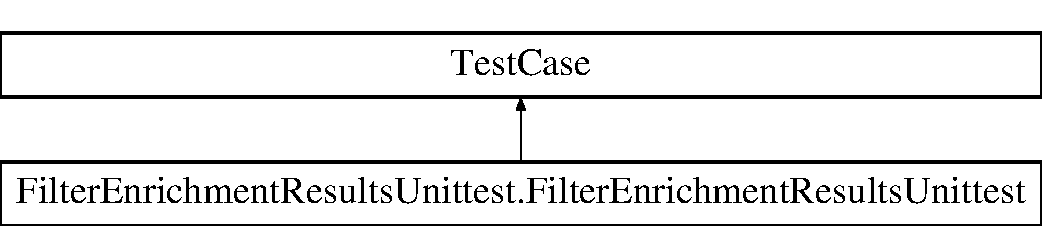
\includegraphics[height=2.000000cm]{classFilterEnrichmentResultsUnittest_1_1FilterEnrichmentResultsUnittest}
\end{center}
\end{figure}
\subsection*{Public Member Functions}
\begin{DoxyCompactItemize}
\item 
\hypertarget{classFilterEnrichmentResultsUnittest_1_1FilterEnrichmentResultsUnittest_aba5123c867674094b36aec8468f3820a}{def {\bfseries set\-Up}}\label{classFilterEnrichmentResultsUnittest_1_1FilterEnrichmentResultsUnittest_aba5123c867674094b36aec8468f3820a}

\item 
\hypertarget{classFilterEnrichmentResultsUnittest_1_1FilterEnrichmentResultsUnittest_a2721b7385680cf4ffddccd7e4fa3969f}{def {\bfseries test\-\_\-read\-\_\-enrichment\-\_\-per\-\_\-rna\-\_\-file}}\label{classFilterEnrichmentResultsUnittest_1_1FilterEnrichmentResultsUnittest_a2721b7385680cf4ffddccd7e4fa3969f}

\item 
\hypertarget{classFilterEnrichmentResultsUnittest_1_1FilterEnrichmentResultsUnittest_a0f4bad70df775ab45f38b968ea1e5343}{def {\bfseries test\-\_\-read\-\_\-enrichment\-\_\-per\-\_\-rna\-\_\-file\-\_\-two}}\label{classFilterEnrichmentResultsUnittest_1_1FilterEnrichmentResultsUnittest_a0f4bad70df775ab45f38b968ea1e5343}

\item 
\hypertarget{classFilterEnrichmentResultsUnittest_1_1FilterEnrichmentResultsUnittest_ac5f2c8e0eebd8f8faec80505dc071378}{def {\bfseries test\-\_\-read\-\_\-enrichment\-\_\-results\-\_\-file}}\label{classFilterEnrichmentResultsUnittest_1_1FilterEnrichmentResultsUnittest_ac5f2c8e0eebd8f8faec80505dc071378}

\item 
\hypertarget{classFilterEnrichmentResultsUnittest_1_1FilterEnrichmentResultsUnittest_ad7dafe90e1b07a84f61bb2c7154c40ec}{def {\bfseries test\-\_\-read\-\_\-enrichment\-\_\-results\-\_\-file\-\_\-two}}\label{classFilterEnrichmentResultsUnittest_1_1FilterEnrichmentResultsUnittest_ad7dafe90e1b07a84f61bb2c7154c40ec}

\item 
\hypertarget{classFilterEnrichmentResultsUnittest_1_1FilterEnrichmentResultsUnittest_a8dc6167564d3aa4f104841c63c462f21}{def {\bfseries test\-\_\-filter\-\_\-by\-\_\-observed\-\_\-interactions}}\label{classFilterEnrichmentResultsUnittest_1_1FilterEnrichmentResultsUnittest_a8dc6167564d3aa4f104841c63c462f21}

\item 
\hypertarget{classFilterEnrichmentResultsUnittest_1_1FilterEnrichmentResultsUnittest_a95744a4c4e94f8b389b847c3d2b0e8bc}{def {\bfseries test\-\_\-run}}\label{classFilterEnrichmentResultsUnittest_1_1FilterEnrichmentResultsUnittest_a95744a4c4e94f8b389b847c3d2b0e8bc}

\item 
\hypertarget{classFilterEnrichmentResultsUnittest_1_1FilterEnrichmentResultsUnittest_aef59299afc8ca4b6714b3a522cc94297}{def {\bfseries test\-\_\-write\-\_\-enrichment\-\_\-results}}\label{classFilterEnrichmentResultsUnittest_1_1FilterEnrichmentResultsUnittest_aef59299afc8ca4b6714b3a522cc94297}

\end{DoxyCompactItemize}
\subsection*{Public Attributes}
\begin{DoxyCompactItemize}
\item 
\hypertarget{classFilterEnrichmentResultsUnittest_1_1FilterEnrichmentResultsUnittest_a12f7cae6473ed09e28c0c15600b89781}{{\bfseries enrichment\-Per\-R\-N\-A\-File}}\label{classFilterEnrichmentResultsUnittest_1_1FilterEnrichmentResultsUnittest_a12f7cae6473ed09e28c0c15600b89781}

\item 
\hypertarget{classFilterEnrichmentResultsUnittest_1_1FilterEnrichmentResultsUnittest_a1ad51636fd7117d63f3fd3ea9dd0d41d}{{\bfseries enrichment\-Results\-File}}\label{classFilterEnrichmentResultsUnittest_1_1FilterEnrichmentResultsUnittest_a1ad51636fd7117d63f3fd3ea9dd0d41d}

\item 
\hypertarget{classFilterEnrichmentResultsUnittest_1_1FilterEnrichmentResultsUnittest_af6d7ea9530c0452d780761ef74cf7447}{{\bfseries output\-Folder}}\label{classFilterEnrichmentResultsUnittest_1_1FilterEnrichmentResultsUnittest_af6d7ea9530c0452d780761ef74cf7447}

\item 
\hypertarget{classFilterEnrichmentResultsUnittest_1_1FilterEnrichmentResultsUnittest_ac4927ca84a8940fea91b2ea556c2ed00}{{\bfseries matrix\-Value\-Column}}\label{classFilterEnrichmentResultsUnittest_1_1FilterEnrichmentResultsUnittest_ac4927ca84a8940fea91b2ea556c2ed00}

\item 
\hypertarget{classFilterEnrichmentResultsUnittest_1_1FilterEnrichmentResultsUnittest_ad99bf3f69d417e611eb6e049bc7db780}{{\bfseries filter\-Warning\-Column}}\label{classFilterEnrichmentResultsUnittest_1_1FilterEnrichmentResultsUnittest_ad99bf3f69d417e611eb6e049bc7db780}

\item 
\hypertarget{classFilterEnrichmentResultsUnittest_1_1FilterEnrichmentResultsUnittest_ab389426c683d6177b4ed8c44576628c1}{{\bfseries filter\-Warning\-Value}}\label{classFilterEnrichmentResultsUnittest_1_1FilterEnrichmentResultsUnittest_ab389426c683d6177b4ed8c44576628c1}

\item 
\hypertarget{classFilterEnrichmentResultsUnittest_1_1FilterEnrichmentResultsUnittest_acffdf280f31c676b63b3938048ce1d66}{{\bfseries minimum\-Ratio}}\label{classFilterEnrichmentResultsUnittest_1_1FilterEnrichmentResultsUnittest_acffdf280f31c676b63b3938048ce1d66}

\item 
\hypertarget{classFilterEnrichmentResultsUnittest_1_1FilterEnrichmentResultsUnittest_ac222b4df068c4ae15246dd2cd87460c2}{{\bfseries row\-Annotation\-File}}\label{classFilterEnrichmentResultsUnittest_1_1FilterEnrichmentResultsUnittest_ac222b4df068c4ae15246dd2cd87460c2}

\item 
\hypertarget{classFilterEnrichmentResultsUnittest_1_1FilterEnrichmentResultsUnittest_a4ec0d18efd9538215eda1b93c3498ed8}{{\bfseries col\-Annotation\-File}}\label{classFilterEnrichmentResultsUnittest_1_1FilterEnrichmentResultsUnittest_a4ec0d18efd9538215eda1b93c3498ed8}

\item 
\hypertarget{classFilterEnrichmentResultsUnittest_1_1FilterEnrichmentResultsUnittest_a0a990191827fabf5802dc5bc01d66288}{{\bfseries mask\-Multiple}}\label{classFilterEnrichmentResultsUnittest_1_1FilterEnrichmentResultsUnittest_a0a990191827fabf5802dc5bc01d66288}

\item 
\hypertarget{classFilterEnrichmentResultsUnittest_1_1FilterEnrichmentResultsUnittest_a78948329c3a73dbe783f0edb76b2c9b7}{{\bfseries no\-Annotation\-Tag}}\label{classFilterEnrichmentResultsUnittest_1_1FilterEnrichmentResultsUnittest_a78948329c3a73dbe783f0edb76b2c9b7}

\item 
\hypertarget{classFilterEnrichmentResultsUnittest_1_1FilterEnrichmentResultsUnittest_a22617dc220bf168a7bbff777930b8ffe}{{\bfseries no\-Annotation\-Filter}}\label{classFilterEnrichmentResultsUnittest_1_1FilterEnrichmentResultsUnittest_a22617dc220bf168a7bbff777930b8ffe}

\item 
\hypertarget{classFilterEnrichmentResultsUnittest_1_1FilterEnrichmentResultsUnittest_ac6470268cd7ed4efa8da2b80283548ed}{{\bfseries annot\-Specificity\-Filter}}\label{classFilterEnrichmentResultsUnittest_1_1FilterEnrichmentResultsUnittest_ac6470268cd7ed4efa8da2b80283548ed}

\item 
\hypertarget{classFilterEnrichmentResultsUnittest_1_1FilterEnrichmentResultsUnittest_a77ea366827f7995db9fd24476b5f5270}{{\bfseries transcript\-Specificity\-Filter}}\label{classFilterEnrichmentResultsUnittest_1_1FilterEnrichmentResultsUnittest_a77ea366827f7995db9fd24476b5f5270}

\item 
\hypertarget{classFilterEnrichmentResultsUnittest_1_1FilterEnrichmentResultsUnittest_ac544ced5864a9065a94812bb84a8a9ca}{{\bfseries minimum\-Protein\-Interaction}}\label{classFilterEnrichmentResultsUnittest_1_1FilterEnrichmentResultsUnittest_ac544ced5864a9065a94812bb84a8a9ca}

\item 
\hypertarget{classFilterEnrichmentResultsUnittest_1_1FilterEnrichmentResultsUnittest_aa386a9a238429c34437d897fcb664778}{{\bfseries top\-Enrichments\-Per\-Complex}}\label{classFilterEnrichmentResultsUnittest_1_1FilterEnrichmentResultsUnittest_aa386a9a238429c34437d897fcb664778}

\item 
\hypertarget{classFilterEnrichmentResultsUnittest_1_1FilterEnrichmentResultsUnittest_ab03839f2c2769127d18c1325b3472756}{{\bfseries run}}\label{classFilterEnrichmentResultsUnittest_1_1FilterEnrichmentResultsUnittest_ab03839f2c2769127d18c1325b3472756}

\item 
\hypertarget{classFilterEnrichmentResultsUnittest_1_1FilterEnrichmentResultsUnittest_aa721ee8d4420c54f8c8b2bdeb58addf3}{\hyperlink{classFilterEnrichmentResultsUnittest_1_1FilterEnrichmentResultsUnittest_aa721ee8d4420c54f8c8b2bdeb58addf3}{expected\-Folder}}\label{classFilterEnrichmentResultsUnittest_1_1FilterEnrichmentResultsUnittest_aa721ee8d4420c54f8c8b2bdeb58addf3}

\begin{DoxyCompactList}\small\item\em A\-D\-D S\-P\-E\-C\-I\-F\-I\-C\-I\-T\-Y A\-N\-D T\-O\-P S\-C\-A\-F\-F\-O\-L\-D F\-I\-L\-T\-E\-R\-S A\-N\-D S\-E\-E I\-F O\-U\-T\-P\-U\-T C\-H\-A\-N\-G\-E\-S Note\-: the filters themselves are not being tested here, just that output file formats look correct. \end{DoxyCompactList}\end{DoxyCompactItemize}


The documentation for this class was generated from the following file\-:\begin{DoxyCompactItemize}
\item 
test/fr/tagc/rainet/core/execution/analysis/\-Enrichment\-Analysis/Filter\-Enrichment\-Results\-Unittest.\-py\end{DoxyCompactItemize}

\hypertarget{classsrc_1_1fr_1_1tagc_1_1rainet_1_1core_1_1data_1_1Gene_1_1Gene}{\section{src.\-fr.\-tagc.\-rainet.\-core.\-data.\-Gene.\-Gene Class Reference}
\label{classsrc_1_1fr_1_1tagc_1_1rainet_1_1core_1_1data_1_1Gene_1_1Gene}\index{src.\-fr.\-tagc.\-rainet.\-core.\-data.\-Gene.\-Gene@{src.\-fr.\-tagc.\-rainet.\-core.\-data.\-Gene.\-Gene}}
}
Inheritance diagram for src.\-fr.\-tagc.\-rainet.\-core.\-data.\-Gene.\-Gene\-:\begin{figure}[H]
\begin{center}
\leavevmode
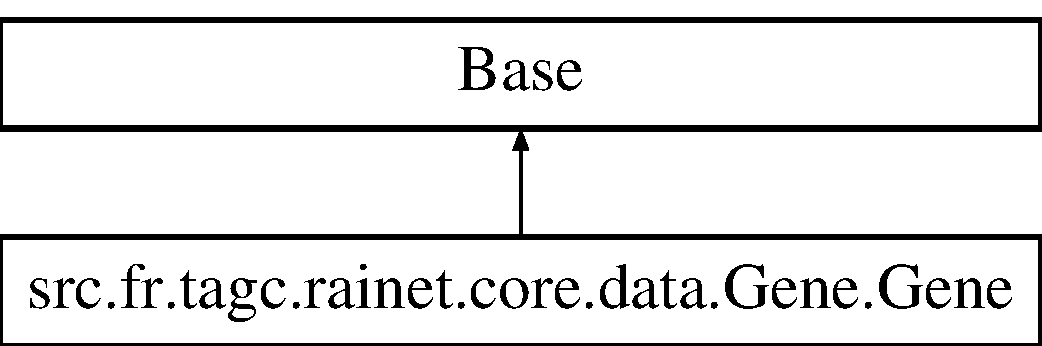
\includegraphics[height=2.000000cm]{classsrc_1_1fr_1_1tagc_1_1rainet_1_1core_1_1data_1_1Gene_1_1Gene}
\end{center}
\end{figure}
\subsection*{Public Member Functions}
\begin{DoxyCompactItemize}
\item 
\hypertarget{classsrc_1_1fr_1_1tagc_1_1rainet_1_1core_1_1data_1_1Gene_1_1Gene_a2d57c0ba3f6f474d04bc3114b5382242}{def {\bfseries \-\_\-\-\_\-init\-\_\-\-\_\-}}\label{classsrc_1_1fr_1_1tagc_1_1rainet_1_1core_1_1data_1_1Gene_1_1Gene_a2d57c0ba3f6f474d04bc3114b5382242}

\item 
\hypertarget{classsrc_1_1fr_1_1tagc_1_1rainet_1_1core_1_1data_1_1Gene_1_1Gene_a6c674ac24c37a47b4e9877bbdb631422}{def {\bfseries add\-\_\-rna}}\label{classsrc_1_1fr_1_1tagc_1_1rainet_1_1core_1_1data_1_1Gene_1_1Gene_a6c674ac24c37a47b4e9877bbdb631422}

\end{DoxyCompactItemize}
\subsection*{Public Attributes}
\begin{DoxyCompactItemize}
\item 
\hypertarget{classsrc_1_1fr_1_1tagc_1_1rainet_1_1core_1_1data_1_1Gene_1_1Gene_aa41848fc9f2bb8d4d7a8acad9cc7b83e}{{\bfseries gene\-I\-D}}\label{classsrc_1_1fr_1_1tagc_1_1rainet_1_1core_1_1data_1_1Gene_1_1Gene_aa41848fc9f2bb8d4d7a8acad9cc7b83e}

\end{DoxyCompactItemize}
\subsection*{Static Public Attributes}
\begin{DoxyCompactItemize}
\item 
\hypertarget{classsrc_1_1fr_1_1tagc_1_1rainet_1_1core_1_1data_1_1Gene_1_1Gene_a11a3ce9ade4324a4daa5258a8c667657}{tuple {\bfseries gene\-I\-D} = Column( String, primary\-\_\-key = True )}\label{classsrc_1_1fr_1_1tagc_1_1rainet_1_1core_1_1data_1_1Gene_1_1Gene_a11a3ce9ade4324a4daa5258a8c667657}

\item 
\hypertarget{classsrc_1_1fr_1_1tagc_1_1rainet_1_1core_1_1data_1_1Gene_1_1Gene_aa55affe2b6fefc7fd5f80eb221b23447}{tuple {\bfseries transcript\-List} = relationship( 'R\-N\-A' , backref=\char`\"{}Gene\char`\"{})}\label{classsrc_1_1fr_1_1tagc_1_1rainet_1_1core_1_1data_1_1Gene_1_1Gene_aa55affe2b6fefc7fd5f80eb221b23447}

\end{DoxyCompactItemize}


The documentation for this class was generated from the following file\-:\begin{DoxyCompactItemize}
\item 
src/fr/tagc/rainet/core/data/Gene.\-py\end{DoxyCompactItemize}

\hypertarget{classsrc_1_1fr_1_1tagc_1_1rainet_1_1core_1_1data_1_1GeneOntology_1_1GeneOntology}{\section{src.\-fr.\-tagc.\-rainet.\-core.\-data.\-Gene\-Ontology.\-Gene\-Ontology Class Reference}
\label{classsrc_1_1fr_1_1tagc_1_1rainet_1_1core_1_1data_1_1GeneOntology_1_1GeneOntology}\index{src.\-fr.\-tagc.\-rainet.\-core.\-data.\-Gene\-Ontology.\-Gene\-Ontology@{src.\-fr.\-tagc.\-rainet.\-core.\-data.\-Gene\-Ontology.\-Gene\-Ontology}}
}


This class describe a gene ontology term.  


Inheritance diagram for src.\-fr.\-tagc.\-rainet.\-core.\-data.\-Gene\-Ontology.\-Gene\-Ontology\-:\begin{figure}[H]
\begin{center}
\leavevmode
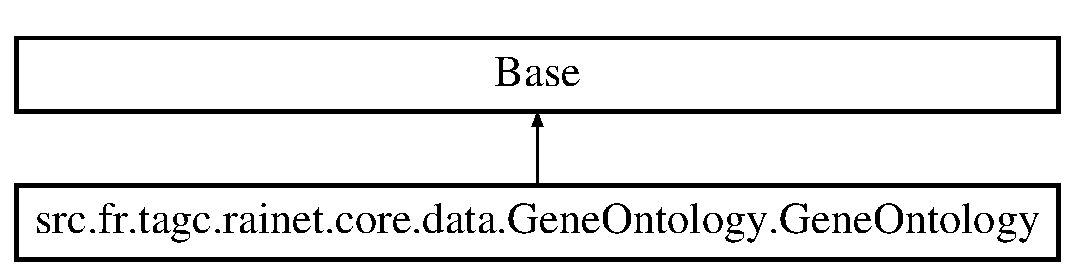
\includegraphics[height=2.000000cm]{classsrc_1_1fr_1_1tagc_1_1rainet_1_1core_1_1data_1_1GeneOntology_1_1GeneOntology}
\end{center}
\end{figure}
\subsection*{Public Member Functions}
\begin{DoxyCompactItemize}
\item 
\hypertarget{classsrc_1_1fr_1_1tagc_1_1rainet_1_1core_1_1data_1_1GeneOntology_1_1GeneOntology_a0e9ab0aaa2d8fbb037f968fee05a619d}{def {\bfseries \-\_\-\-\_\-init\-\_\-\-\_\-}}\label{classsrc_1_1fr_1_1tagc_1_1rainet_1_1core_1_1data_1_1GeneOntology_1_1GeneOntology_a0e9ab0aaa2d8fbb037f968fee05a619d}

\item 
\hypertarget{classsrc_1_1fr_1_1tagc_1_1rainet_1_1core_1_1data_1_1GeneOntology_1_1GeneOntology_ac1d929697335fd2bfe10b406e6952bfe}{def \hyperlink{classsrc_1_1fr_1_1tagc_1_1rainet_1_1core_1_1data_1_1GeneOntology_1_1GeneOntology_ac1d929697335fd2bfe10b406e6952bfe}{add\-\_\-annotated\-\_\-protein}}\label{classsrc_1_1fr_1_1tagc_1_1rainet_1_1core_1_1data_1_1GeneOntology_1_1GeneOntology_ac1d929697335fd2bfe10b406e6952bfe}

\begin{DoxyCompactList}\small\item\em Add an annotated protein to the list. \end{DoxyCompactList}\end{DoxyCompactItemize}
\subsection*{Public Attributes}
\begin{DoxyCompactItemize}
\item 
\hypertarget{classsrc_1_1fr_1_1tagc_1_1rainet_1_1core_1_1data_1_1GeneOntology_1_1GeneOntology_a76e20a64bab3d9dd26e233225386dd56}{{\bfseries go\-I\-D}}\label{classsrc_1_1fr_1_1tagc_1_1rainet_1_1core_1_1data_1_1GeneOntology_1_1GeneOntology_a76e20a64bab3d9dd26e233225386dd56}

\item 
\hypertarget{classsrc_1_1fr_1_1tagc_1_1rainet_1_1core_1_1data_1_1GeneOntology_1_1GeneOntology_a4deef56f246373285d8e50bf16cf22b3}{{\bfseries go\-Term}}\label{classsrc_1_1fr_1_1tagc_1_1rainet_1_1core_1_1data_1_1GeneOntology_1_1GeneOntology_a4deef56f246373285d8e50bf16cf22b3}

\item 
\hypertarget{classsrc_1_1fr_1_1tagc_1_1rainet_1_1core_1_1data_1_1GeneOntology_1_1GeneOntology_a06a9a5c549eb766c7fc9c7f0ac4a61e4}{{\bfseries go\-Aspect}}\label{classsrc_1_1fr_1_1tagc_1_1rainet_1_1core_1_1data_1_1GeneOntology_1_1GeneOntology_a06a9a5c549eb766c7fc9c7f0ac4a61e4}

\end{DoxyCompactItemize}
\subsection*{Static Public Attributes}
\begin{DoxyCompactItemize}
\item 
\hypertarget{classsrc_1_1fr_1_1tagc_1_1rainet_1_1core_1_1data_1_1GeneOntology_1_1GeneOntology_a55e56b33490195397547c192cea5f7ed}{tuple {\bfseries go\-I\-D} = Column( String, primary\-\_\-key = True )}\label{classsrc_1_1fr_1_1tagc_1_1rainet_1_1core_1_1data_1_1GeneOntology_1_1GeneOntology_a55e56b33490195397547c192cea5f7ed}

\item 
\hypertarget{classsrc_1_1fr_1_1tagc_1_1rainet_1_1core_1_1data_1_1GeneOntology_1_1GeneOntology_a48f0ec4d3d50a09f615ea80db3924582}{tuple {\bfseries go\-Term} = Column( String )}\label{classsrc_1_1fr_1_1tagc_1_1rainet_1_1core_1_1data_1_1GeneOntology_1_1GeneOntology_a48f0ec4d3d50a09f615ea80db3924582}

\item 
\hypertarget{classsrc_1_1fr_1_1tagc_1_1rainet_1_1core_1_1data_1_1GeneOntology_1_1GeneOntology_a4476e0800ca3ab0b2a74355041ab79ca}{tuple {\bfseries go\-Aspect} = Column( String)}\label{classsrc_1_1fr_1_1tagc_1_1rainet_1_1core_1_1data_1_1GeneOntology_1_1GeneOntology_a4476e0800ca3ab0b2a74355041ab79ca}

\item 
\hypertarget{classsrc_1_1fr_1_1tagc_1_1rainet_1_1core_1_1data_1_1GeneOntology_1_1GeneOntology_a97b454c923caabc177005978897bafb6}{tuple {\bfseries annotated\-Proteins} = relationship('Protein', secondary=Protein\-G\-O\-Annotation.\-\_\-\-\_\-table\-\_\-\-\_\-, backref=\char`\"{}go\-Annotations\char`\"{})}\label{classsrc_1_1fr_1_1tagc_1_1rainet_1_1core_1_1data_1_1GeneOntology_1_1GeneOntology_a97b454c923caabc177005978897bafb6}

\end{DoxyCompactItemize}


\subsection{Detailed Description}
This class describe a gene ontology term. 

The documentation for this class was generated from the following file\-:\begin{DoxyCompactItemize}
\item 
src/fr/tagc/rainet/core/data/Gene\-Ontology.\-py\end{DoxyCompactItemize}

\hypertarget{classsrc_1_1fr_1_1tagc_1_1rainet_1_1core_1_1data_1_1GeneSymbol_1_1GeneSymbol}{\section{src.\-fr.\-tagc.\-rainet.\-core.\-data.\-Gene\-Symbol.\-Gene\-Symbol Class Reference}
\label{classsrc_1_1fr_1_1tagc_1_1rainet_1_1core_1_1data_1_1GeneSymbol_1_1GeneSymbol}\index{src.\-fr.\-tagc.\-rainet.\-core.\-data.\-Gene\-Symbol.\-Gene\-Symbol@{src.\-fr.\-tagc.\-rainet.\-core.\-data.\-Gene\-Symbol.\-Gene\-Symbol}}
}


This class describe a gene symbol associated to a protein this class has a many-\/to-\/one relationship with the class Protein.  


Inheritance diagram for src.\-fr.\-tagc.\-rainet.\-core.\-data.\-Gene\-Symbol.\-Gene\-Symbol\-:\begin{figure}[H]
\begin{center}
\leavevmode
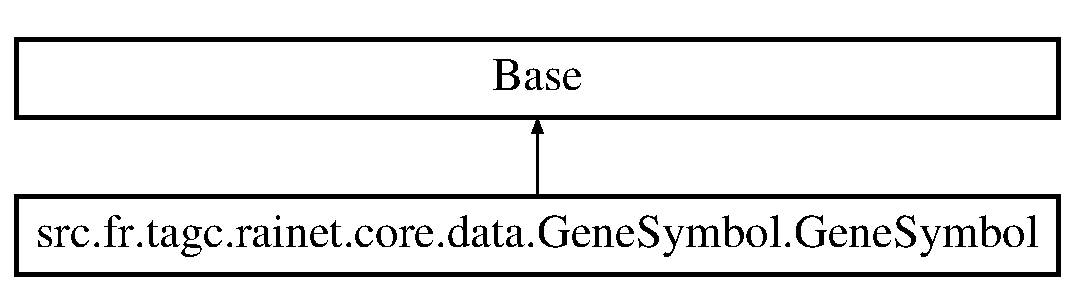
\includegraphics[height=2.000000cm]{classsrc_1_1fr_1_1tagc_1_1rainet_1_1core_1_1data_1_1GeneSymbol_1_1GeneSymbol}
\end{center}
\end{figure}
\subsection*{Public Member Functions}
\begin{DoxyCompactItemize}
\item 
\hypertarget{classsrc_1_1fr_1_1tagc_1_1rainet_1_1core_1_1data_1_1GeneSymbol_1_1GeneSymbol_a65846cbf33fbd102348042e83077ad85}{def \hyperlink{classsrc_1_1fr_1_1tagc_1_1rainet_1_1core_1_1data_1_1GeneSymbol_1_1GeneSymbol_a65846cbf33fbd102348042e83077ad85}{add\-\_\-synonym}}\label{classsrc_1_1fr_1_1tagc_1_1rainet_1_1core_1_1data_1_1GeneSymbol_1_1GeneSymbol_a65846cbf33fbd102348042e83077ad85}

\begin{DoxyCompactList}\small\item\em Add a Synonym\-Gene\-Symbol to the list. \end{DoxyCompactList}\end{DoxyCompactItemize}
\subsection*{Static Public Attributes}
\begin{DoxyCompactItemize}
\item 
\hypertarget{classsrc_1_1fr_1_1tagc_1_1rainet_1_1core_1_1data_1_1GeneSymbol_1_1GeneSymbol_ad9748883488bebb33beb35ab9471f795}{tuple {\bfseries protein\-\_\-id} = Column( String, Foreign\-Key('Protein.\-uniprot\-A\-C'))}\label{classsrc_1_1fr_1_1tagc_1_1rainet_1_1core_1_1data_1_1GeneSymbol_1_1GeneSymbol_ad9748883488bebb33beb35ab9471f795}

\item 
\hypertarget{classsrc_1_1fr_1_1tagc_1_1rainet_1_1core_1_1data_1_1GeneSymbol_1_1GeneSymbol_aa77854e15fce296866c9b787b1c8c0bd}{tuple {\bfseries uniprot\-Gene\-Symbol} = Column( String)}\label{classsrc_1_1fr_1_1tagc_1_1rainet_1_1core_1_1data_1_1GeneSymbol_1_1GeneSymbol_aa77854e15fce296866c9b787b1c8c0bd}

\item 
\hypertarget{classsrc_1_1fr_1_1tagc_1_1rainet_1_1core_1_1data_1_1GeneSymbol_1_1GeneSymbol_a7d824769d94ed91633de9c4631f93fe0}{tuple {\bfseries uniprot\-Synonym\-Gene\-Symbols} = relationship( 'Synonym\-Gene\-Symbol', backref = 'gene\-Symbol' )}\label{classsrc_1_1fr_1_1tagc_1_1rainet_1_1core_1_1data_1_1GeneSymbol_1_1GeneSymbol_a7d824769d94ed91633de9c4631f93fe0}

\end{DoxyCompactItemize}


\subsection{Detailed Description}
This class describe a gene symbol associated to a protein this class has a many-\/to-\/one relationship with the class Protein. 

The documentation for this class was generated from the following file\-:\begin{DoxyCompactItemize}
\item 
src/fr/tagc/rainet/core/data/Gene\-Symbol.\-py\end{DoxyCompactItemize}

\hypertarget{classsrc_1_1core_1_1util_1_1tools_1_1GlobalOverlapRegionAnalysis_1_1GlobalOverlapRegionAnalysis}{\section{src.\-core.\-util.\-tools.\-Global\-Overlap\-Region\-Analysis.\-Global\-Overlap\-Region\-Analysis Class Reference}
\label{classsrc_1_1core_1_1util_1_1tools_1_1GlobalOverlapRegionAnalysis_1_1GlobalOverlapRegionAnalysis}\index{src.\-core.\-util.\-tools.\-Global\-Overlap\-Region\-Analysis.\-Global\-Overlap\-Region\-Analysis@{src.\-core.\-util.\-tools.\-Global\-Overlap\-Region\-Analysis.\-Global\-Overlap\-Region\-Analysis}}
}
\subsection*{Static Public Member Functions}
\begin{DoxyCompactItemize}
\item 
\hypertarget{classsrc_1_1core_1_1util_1_1tools_1_1GlobalOverlapRegionAnalysis_1_1GlobalOverlapRegionAnalysis_a72142d765cf144f7022e01a521d0511c}{def {\bfseries overlap\-\_\-file\-\_\-write}}\label{classsrc_1_1core_1_1util_1_1tools_1_1GlobalOverlapRegionAnalysis_1_1GlobalOverlapRegionAnalysis_a72142d765cf144f7022e01a521d0511c}

\item 
\hypertarget{classsrc_1_1core_1_1util_1_1tools_1_1GlobalOverlapRegionAnalysis_1_1GlobalOverlapRegionAnalysis_a5f4f19906a0a821a9f0b0e172f123ffe}{def {\bfseries iupred\-\_\-overlap\-\_\-analysis}}\label{classsrc_1_1core_1_1util_1_1tools_1_1GlobalOverlapRegionAnalysis_1_1GlobalOverlapRegionAnalysis_a5f4f19906a0a821a9f0b0e172f123ffe}

\item 
\hypertarget{classsrc_1_1core_1_1util_1_1tools_1_1GlobalOverlapRegionAnalysis_1_1GlobalOverlapRegionAnalysis_a75f513dd37e03dccb4aa28224116b084}{def {\bfseries anchor\-\_\-overlap\-\_\-analysis}}\label{classsrc_1_1core_1_1util_1_1tools_1_1GlobalOverlapRegionAnalysis_1_1GlobalOverlapRegionAnalysis_a75f513dd37e03dccb4aa28224116b084}

\item 
\hypertarget{classsrc_1_1core_1_1util_1_1tools_1_1GlobalOverlapRegionAnalysis_1_1GlobalOverlapRegionAnalysis_a38768040889ebade6a04eb62dfa6ad86}{def {\bfseries disordp\-\_\-overlap\-\_\-analysis}}\label{classsrc_1_1core_1_1util_1_1tools_1_1GlobalOverlapRegionAnalysis_1_1GlobalOverlapRegionAnalysis_a38768040889ebade6a04eb62dfa6ad86}

\end{DoxyCompactItemize}


The documentation for this class was generated from the following file\-:\begin{DoxyCompactItemize}
\item 
rbp-\/motif/src/core/util/tools/Global\-Overlap\-Region\-Analysis.\-py\end{DoxyCompactItemize}

\hypertarget{classGroupOddsRatio_1_1GroupOddsRatio}{\section{Group\-Odds\-Ratio.\-Group\-Odds\-Ratio Class Reference}
\label{classGroupOddsRatio_1_1GroupOddsRatio}\index{Group\-Odds\-Ratio.\-Group\-Odds\-Ratio@{Group\-Odds\-Ratio.\-Group\-Odds\-Ratio}}
}
Inheritance diagram for Group\-Odds\-Ratio.\-Group\-Odds\-Ratio\-:\begin{figure}[H]
\begin{center}
\leavevmode
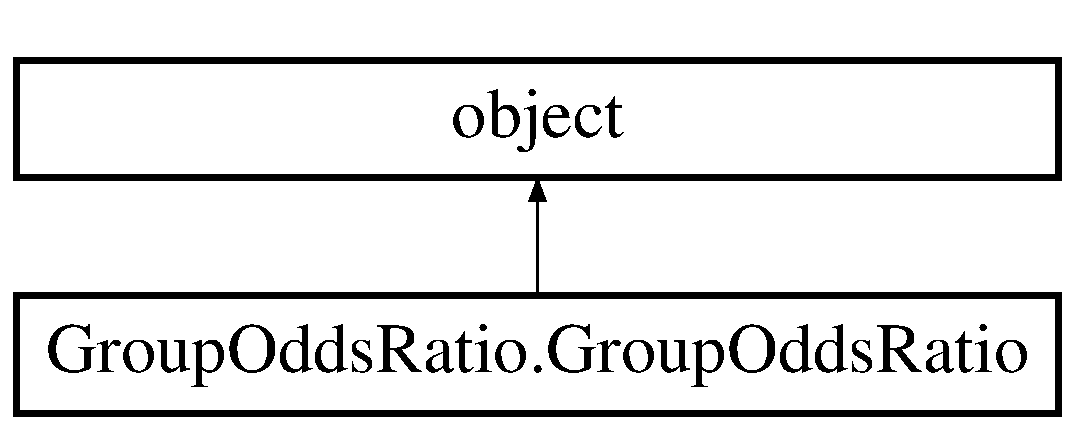
\includegraphics[height=2.000000cm]{classGroupOddsRatio_1_1GroupOddsRatio}
\end{center}
\end{figure}
\subsection*{Public Member Functions}
\begin{DoxyCompactItemize}
\item 
\hypertarget{classGroupOddsRatio_1_1GroupOddsRatio_aec69e18faa9a51522959f3dd9d5e538a}{def {\bfseries \-\_\-\-\_\-init\-\_\-\-\_\-}}\label{classGroupOddsRatio_1_1GroupOddsRatio_aec69e18faa9a51522959f3dd9d5e538a}

\item 
\hypertarget{classGroupOddsRatio_1_1GroupOddsRatio_ae1c6859406f05f270493ddc544b2bd53}{def {\bfseries read\-\_\-annotation\-\_\-file}}\label{classGroupOddsRatio_1_1GroupOddsRatio_ae1c6859406f05f270493ddc544b2bd53}

\item 
\hypertarget{classGroupOddsRatio_1_1GroupOddsRatio_af8a83aca2f1e4cff694e7eff001f4aee}{def {\bfseries read\-\_\-external\-\_\-files}}\label{classGroupOddsRatio_1_1GroupOddsRatio_af8a83aca2f1e4cff694e7eff001f4aee}

\item 
\hypertarget{classGroupOddsRatio_1_1GroupOddsRatio_a28c9307316b82a27b0899909e95ef0b0}{def {\bfseries read\-\_\-background\-\_\-list}}\label{classGroupOddsRatio_1_1GroupOddsRatio_a28c9307316b82a27b0899909e95ef0b0}

\item 
\hypertarget{classGroupOddsRatio_1_1GroupOddsRatio_aa060f2c1b8b606d7dc814251b254060a}{def {\bfseries calculate\-\_\-odds\-\_\-ratio}}\label{classGroupOddsRatio_1_1GroupOddsRatio_aa060f2c1b8b606d7dc814251b254060a}

\item 
\hypertarget{classGroupOddsRatio_1_1GroupOddsRatio_ad9d7e1b0c5e90275c88a074c7cb40b95}{def {\bfseries run}}\label{classGroupOddsRatio_1_1GroupOddsRatio_ad9d7e1b0c5e90275c88a074c7cb40b95}

\end{DoxyCompactItemize}
\subsection*{Static Public Member Functions}
\begin{DoxyCompactItemize}
\item 
\hypertarget{classGroupOddsRatio_1_1GroupOddsRatio_abcf2a4fb2fb97c0e67ab09ac2d173186}{def {\bfseries fisher\-\_\-exact\-\_\-test}}\label{classGroupOddsRatio_1_1GroupOddsRatio_abcf2a4fb2fb97c0e67ab09ac2d173186}

\end{DoxyCompactItemize}
\subsection*{Public Attributes}
\begin{DoxyCompactItemize}
\item 
\hypertarget{classGroupOddsRatio_1_1GroupOddsRatio_a95d8128e7fadbfeecf5574a1948d5007}{{\bfseries annotation\-File}}\label{classGroupOddsRatio_1_1GroupOddsRatio_a95d8128e7fadbfeecf5574a1948d5007}

\item 
\hypertarget{classGroupOddsRatio_1_1GroupOddsRatio_aed00835777234db9526bfce190ec0323}{{\bfseries external\-Files}}\label{classGroupOddsRatio_1_1GroupOddsRatio_aed00835777234db9526bfce190ec0323}

\item 
\hypertarget{classGroupOddsRatio_1_1GroupOddsRatio_ac6719d1ab33663a7d851e96a63d1f64a}{{\bfseries background\-List}}\label{classGroupOddsRatio_1_1GroupOddsRatio_ac6719d1ab33663a7d851e96a63d1f64a}

\item 
\hypertarget{classGroupOddsRatio_1_1GroupOddsRatio_aea816fc10148c6500f8601de55df50a7}{{\bfseries output\-File}}\label{classGroupOddsRatio_1_1GroupOddsRatio_aea816fc10148c6500f8601de55df50a7}

\item 
\hypertarget{classGroupOddsRatio_1_1GroupOddsRatio_a5c764fdbd9e3c52834882220c8064a0d}{{\bfseries item\-Annotation}}\label{classGroupOddsRatio_1_1GroupOddsRatio_a5c764fdbd9e3c52834882220c8064a0d}

\item 
\hypertarget{classGroupOddsRatio_1_1GroupOddsRatio_abdf82605ade4b85a1662640a95d42ff6}{{\bfseries group\-Items}}\label{classGroupOddsRatio_1_1GroupOddsRatio_abdf82605ade4b85a1662640a95d42ff6}

\item 
\hypertarget{classGroupOddsRatio_1_1GroupOddsRatio_a1d9561c3bc16df236b1ad08cfb0839bc}{{\bfseries external\-Lists}}\label{classGroupOddsRatio_1_1GroupOddsRatio_a1d9561c3bc16df236b1ad08cfb0839bc}

\item 
\hyperlink{classGroupOddsRatio_1_1GroupOddsRatio_a4655bff46e55b7dd0d726415726b4dd8}{background\-Items}
\begin{DoxyCompactList}\small\item\em annotation items \end{DoxyCompactList}\item 
\hypertarget{classGroupOddsRatio_1_1GroupOddsRatio_a7b8a8806bcbc063b7962eb8613241d0f}{{\bfseries filtered\-External\-Lists}}\label{classGroupOddsRatio_1_1GroupOddsRatio_a7b8a8806bcbc063b7962eb8613241d0f}

\item 
\hypertarget{classGroupOddsRatio_1_1GroupOddsRatio_ac3fb5ddcbcd90c2c370b27e078f83459}{{\bfseries filtered\-Annotation\-Items}}\label{classGroupOddsRatio_1_1GroupOddsRatio_ac3fb5ddcbcd90c2c370b27e078f83459}

\item 
\hypertarget{classGroupOddsRatio_1_1GroupOddsRatio_a6ac34a0d256191a5c7af5a776bff359b}{{\bfseries data\-Store}}\label{classGroupOddsRatio_1_1GroupOddsRatio_a6ac34a0d256191a5c7af5a776bff359b}

\end{DoxyCompactItemize}
\subsection*{Static Public Attributes}
\begin{DoxyCompactItemize}
\item 
\hypertarget{classGroupOddsRatio_1_1GroupOddsRatio_adcb99c1a1280e2b72f4708ee029bd335}{int {\bfseries A\-N\-N\-O\-T\-A\-T\-I\-O\-N\-\_\-\-F\-I\-L\-E\-\_\-\-I\-D\-\_\-\-C\-O\-L\-U\-M\-N} = 0}\label{classGroupOddsRatio_1_1GroupOddsRatio_adcb99c1a1280e2b72f4708ee029bd335}

\item 
\hypertarget{classGroupOddsRatio_1_1GroupOddsRatio_a7b01b7fd263130f7f43297fc7d4f8615}{int {\bfseries A\-N\-N\-O\-T\-A\-T\-I\-O\-N\-\_\-\-F\-I\-L\-E\-\_\-\-A\-N\-N\-O\-T\-A\-T\-I\-O\-N\-\_\-\-C\-O\-L\-U\-M\-N} = 1}\label{classGroupOddsRatio_1_1GroupOddsRatio_a7b01b7fd263130f7f43297fc7d4f8615}

\end{DoxyCompactItemize}


\subsection{Member Data Documentation}
\hypertarget{classGroupOddsRatio_1_1GroupOddsRatio_a4655bff46e55b7dd0d726415726b4dd8}{\index{Group\-Odds\-Ratio\-::\-Group\-Odds\-Ratio@{Group\-Odds\-Ratio\-::\-Group\-Odds\-Ratio}!background\-Items@{background\-Items}}
\index{background\-Items@{background\-Items}!GroupOddsRatio::GroupOddsRatio@{Group\-Odds\-Ratio\-::\-Group\-Odds\-Ratio}}
\subsubsection[{background\-Items}]{\setlength{\rightskip}{0pt plus 5cm}Group\-Odds\-Ratio.\-Group\-Odds\-Ratio.\-background\-Items}}\label{classGroupOddsRatio_1_1GroupOddsRatio_a4655bff46e55b7dd0d726415726b4dd8}


annotation items 

External item lists 

The documentation for this class was generated from the following file\-:\begin{DoxyCompactItemize}
\item 
src/fr/tagc/rainet/core/execution/analysis/\-R\-B\-P\-Domain/Group\-Odds\-Ratio.\-py\end{DoxyCompactItemize}

\hypertarget{classsrc_1_1core_1_1util_1_1format_1_1HeaderParser_1_1HeaderParser}{\section{src.\-core.\-util.\-format.\-Header\-Parser.\-Header\-Parser Class Reference}
\label{classsrc_1_1core_1_1util_1_1format_1_1HeaderParser_1_1HeaderParser}\index{src.\-core.\-util.\-format.\-Header\-Parser.\-Header\-Parser@{src.\-core.\-util.\-format.\-Header\-Parser.\-Header\-Parser}}
}
\subsection*{Static Public Member Functions}
\begin{DoxyCompactItemize}
\item 
\hypertarget{classsrc_1_1core_1_1util_1_1format_1_1HeaderParser_1_1HeaderParser_a6c41c1ac672a1ae535fdd00ec450bdc7}{def {\bfseries change\-\_\-header}}\label{classsrc_1_1core_1_1util_1_1format_1_1HeaderParser_1_1HeaderParser_a6c41c1ac672a1ae535fdd00ec450bdc7}

\end{DoxyCompactItemize}


The documentation for this class was generated from the following file\-:\begin{DoxyCompactItemize}
\item 
rbp-\/motif/src/core/util/format/Header\-Parser.\-py\end{DoxyCompactItemize}

\hypertarget{classsrc_1_1core_1_1util_1_1dataset_1_1InfoDataset_1_1InfoDataset}{\section{src.\-core.\-util.\-dataset.\-Info\-Dataset.\-Info\-Dataset Class Reference}
\label{classsrc_1_1core_1_1util_1_1dataset_1_1InfoDataset_1_1InfoDataset}\index{src.\-core.\-util.\-dataset.\-Info\-Dataset.\-Info\-Dataset@{src.\-core.\-util.\-dataset.\-Info\-Dataset.\-Info\-Dataset}}
}
\subsection*{Static Public Member Functions}
\begin{DoxyCompactItemize}
\item 
\hypertarget{classsrc_1_1core_1_1util_1_1dataset_1_1InfoDataset_1_1InfoDataset_a7fb531ab9e97f87deb649e5066f73680}{def {\bfseries get\-\_\-dataset\-\_\-feature}}\label{classsrc_1_1core_1_1util_1_1dataset_1_1InfoDataset_1_1InfoDataset_a7fb531ab9e97f87deb649e5066f73680}

\item 
\hypertarget{classsrc_1_1core_1_1util_1_1dataset_1_1InfoDataset_1_1InfoDataset_aa17b02ebb653e27a737746f36e201329}{def {\bfseries check\-\_\-length}}\label{classsrc_1_1core_1_1util_1_1dataset_1_1InfoDataset_1_1InfoDataset_aa17b02ebb653e27a737746f36e201329}

\item 
\hypertarget{classsrc_1_1core_1_1util_1_1dataset_1_1InfoDataset_1_1InfoDataset_aed2df9b2fba173f23b7cbd1187c9c42f}{def {\bfseries comparison\-\_\-dataset}}\label{classsrc_1_1core_1_1util_1_1dataset_1_1InfoDataset_1_1InfoDataset_aed2df9b2fba173f23b7cbd1187c9c42f}

\item 
\hypertarget{classsrc_1_1core_1_1util_1_1dataset_1_1InfoDataset_1_1InfoDataset_a839ef0f3ae011b5875439d0193ce063c}{def {\bfseries global\-\_\-analysis\-\_\-dataset}}\label{classsrc_1_1core_1_1util_1_1dataset_1_1InfoDataset_1_1InfoDataset_a839ef0f3ae011b5875439d0193ce063c}

\end{DoxyCompactItemize}


The documentation for this class was generated from the following file\-:\begin{DoxyCompactItemize}
\item 
rbp-\/motif/src/core/util/dataset/Info\-Dataset.\-py\end{DoxyCompactItemize}

\hypertarget{classsrc_1_1core_1_1util_1_1format_1_1InfoFasta_1_1InfoFasta}{\section{src.\-core.\-util.\-format.\-Info\-Fasta.\-Info\-Fasta Class Reference}
\label{classsrc_1_1core_1_1util_1_1format_1_1InfoFasta_1_1InfoFasta}\index{src.\-core.\-util.\-format.\-Info\-Fasta.\-Info\-Fasta@{src.\-core.\-util.\-format.\-Info\-Fasta.\-Info\-Fasta}}
}
\subsection*{Static Public Member Functions}
\begin{DoxyCompactItemize}
\item 
\hypertarget{classsrc_1_1core_1_1util_1_1format_1_1InfoFasta_1_1InfoFasta_a8fa1175c763a5a321dd73e2908fd71f1}{def {\bfseries get\-\_\-header}}\label{classsrc_1_1core_1_1util_1_1format_1_1InfoFasta_1_1InfoFasta_a8fa1175c763a5a321dd73e2908fd71f1}

\item 
\hypertarget{classsrc_1_1core_1_1util_1_1format_1_1InfoFasta_1_1InfoFasta_a87b84fb11b0a5ab4f6ca46da6de2c7e7}{def {\bfseries get\-\_\-seq}}\label{classsrc_1_1core_1_1util_1_1format_1_1InfoFasta_1_1InfoFasta_a87b84fb11b0a5ab4f6ca46da6de2c7e7}

\item 
\hypertarget{classsrc_1_1core_1_1util_1_1format_1_1InfoFasta_1_1InfoFasta_a905fc69686c91a48b7f368379698614f}{def {\bfseries get\-\_\-length}}\label{classsrc_1_1core_1_1util_1_1format_1_1InfoFasta_1_1InfoFasta_a905fc69686c91a48b7f368379698614f}

\item 
\hypertarget{classsrc_1_1core_1_1util_1_1format_1_1InfoFasta_1_1InfoFasta_a15d33594e95c385efaffcdc0ec3f694d}{def {\bfseries make\-\_\-dictionary}}\label{classsrc_1_1core_1_1util_1_1format_1_1InfoFasta_1_1InfoFasta_a15d33594e95c385efaffcdc0ec3f694d}

\end{DoxyCompactItemize}


The documentation for this class was generated from the following file\-:\begin{DoxyCompactItemize}
\item 
rbp-\/motif/src/core/util/format/Info\-Fasta.\-py\end{DoxyCompactItemize}

\hypertarget{classsrc_1_1fr_1_1tagc_1_1rainet_1_1core_1_1execution_1_1InsertionStrategy_1_1InsertionStrategy}{\section{src.\-fr.\-tagc.\-rainet.\-core.\-execution.\-Insertion\-Strategy.\-Insertion\-Strategy Class Reference}
\label{classsrc_1_1fr_1_1tagc_1_1rainet_1_1core_1_1execution_1_1InsertionStrategy_1_1InsertionStrategy}\index{src.\-fr.\-tagc.\-rainet.\-core.\-execution.\-Insertion\-Strategy.\-Insertion\-Strategy@{src.\-fr.\-tagc.\-rainet.\-core.\-execution.\-Insertion\-Strategy.\-Insertion\-Strategy}}
}
Inheritance diagram for src.\-fr.\-tagc.\-rainet.\-core.\-execution.\-Insertion\-Strategy.\-Insertion\-Strategy\-:\begin{figure}[H]
\begin{center}
\leavevmode
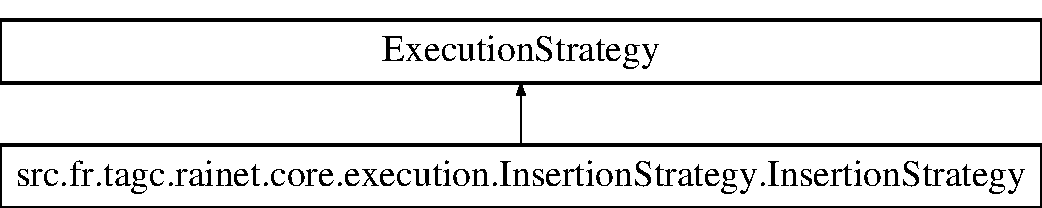
\includegraphics[height=2.000000cm]{classsrc_1_1fr_1_1tagc_1_1rainet_1_1core_1_1execution_1_1InsertionStrategy_1_1InsertionStrategy}
\end{center}
\end{figure}
\subsection*{Public Member Functions}
\begin{DoxyCompactItemize}
\item 
\hypertarget{classsrc_1_1fr_1_1tagc_1_1rainet_1_1core_1_1execution_1_1InsertionStrategy_1_1InsertionStrategy_adaf3ffb94c2b2db37217354bfecb35e3}{def {\bfseries execute}}\label{classsrc_1_1fr_1_1tagc_1_1rainet_1_1core_1_1execution_1_1InsertionStrategy_1_1InsertionStrategy_adaf3ffb94c2b2db37217354bfecb35e3}

\item 
\hypertarget{classsrc_1_1fr_1_1tagc_1_1rainet_1_1core_1_1execution_1_1InsertionStrategy_1_1InsertionStrategy_acf44d09a50112513c1df74f1ea61b645}{def {\bfseries insert\-\_\-data}}\label{classsrc_1_1fr_1_1tagc_1_1rainet_1_1core_1_1execution_1_1InsertionStrategy_1_1InsertionStrategy_acf44d09a50112513c1df74f1ea61b645}

\item 
\hypertarget{classsrc_1_1fr_1_1tagc_1_1rainet_1_1core_1_1execution_1_1InsertionStrategy_1_1InsertionStrategy_a7e793c610ef06be5216b197b3db3b9cf}{def {\bfseries launch\-\_\-insertion\-\_\-\-T\-S\-V}}\label{classsrc_1_1fr_1_1tagc_1_1rainet_1_1core_1_1execution_1_1InsertionStrategy_1_1InsertionStrategy_a7e793c610ef06be5216b197b3db3b9cf}

\item 
\hypertarget{classsrc_1_1fr_1_1tagc_1_1rainet_1_1core_1_1execution_1_1InsertionStrategy_1_1InsertionStrategy_a8628df5ce8d7b9e46786d3faeb90e10d}{def {\bfseries launch\-\_\-insertion\-\_\-\-Network\-Module}}\label{classsrc_1_1fr_1_1tagc_1_1rainet_1_1core_1_1execution_1_1InsertionStrategy_1_1InsertionStrategy_a8628df5ce8d7b9e46786d3faeb90e10d}

\item 
\hypertarget{classsrc_1_1fr_1_1tagc_1_1rainet_1_1core_1_1execution_1_1InsertionStrategy_1_1InsertionStrategy_ab5957555e92b2a13466f3008655defc2}{def {\bfseries launch\-\_\-insertion\-\_\-\-Network\-Module\-Annotation}}\label{classsrc_1_1fr_1_1tagc_1_1rainet_1_1core_1_1execution_1_1InsertionStrategy_1_1InsertionStrategy_ab5957555e92b2a13466f3008655defc2}

\item 
\hypertarget{classsrc_1_1fr_1_1tagc_1_1rainet_1_1core_1_1execution_1_1InsertionStrategy_1_1InsertionStrategy_aec8867b068351bccbc9d03e819b59ccf}{def {\bfseries launch\-\_\-insertion\-\_\-\-Obo}}\label{classsrc_1_1fr_1_1tagc_1_1rainet_1_1core_1_1execution_1_1InsertionStrategy_1_1InsertionStrategy_aec8867b068351bccbc9d03e819b59ccf}

\item 
\hypertarget{classsrc_1_1fr_1_1tagc_1_1rainet_1_1core_1_1execution_1_1InsertionStrategy_1_1InsertionStrategy_a43f45e6ef3409076e0fd2264ef72b1d9}{def {\bfseries launch\-\_\-insertion\-\_\-\-Fasta}}\label{classsrc_1_1fr_1_1tagc_1_1rainet_1_1core_1_1execution_1_1InsertionStrategy_1_1InsertionStrategy_a43f45e6ef3409076e0fd2264ef72b1d9}

\item 
\hypertarget{classsrc_1_1fr_1_1tagc_1_1rainet_1_1core_1_1execution_1_1InsertionStrategy_1_1InsertionStrategy_aab6a63e5f9e354608d6b6770f40a51d2}{def {\bfseries check\-\_\-database\-\_\-tables}}\label{classsrc_1_1fr_1_1tagc_1_1rainet_1_1core_1_1execution_1_1InsertionStrategy_1_1InsertionStrategy_aab6a63e5f9e354608d6b6770f40a51d2}

\end{DoxyCompactItemize}
\subsection*{Public Attributes}
\begin{DoxyCompactItemize}
\item 
\hypertarget{classsrc_1_1fr_1_1tagc_1_1rainet_1_1core_1_1execution_1_1InsertionStrategy_1_1InsertionStrategy_ae5da54a1355b5e93dd5a02b63b83a3bd}{{\bfseries D\-B\-Path}}\label{classsrc_1_1fr_1_1tagc_1_1rainet_1_1core_1_1execution_1_1InsertionStrategy_1_1InsertionStrategy_ae5da54a1355b5e93dd5a02b63b83a3bd}

\item 
\hypertarget{classsrc_1_1fr_1_1tagc_1_1rainet_1_1core_1_1execution_1_1InsertionStrategy_1_1InsertionStrategy_a3187f3fe8396253a147a511102489ac5}{{\bfseries force\-Override}}\label{classsrc_1_1fr_1_1tagc_1_1rainet_1_1core_1_1execution_1_1InsertionStrategy_1_1InsertionStrategy_a3187f3fe8396253a147a511102489ac5}

\end{DoxyCompactItemize}


The documentation for this class was generated from the following file\-:\begin{DoxyCompactItemize}
\item 
src/fr/tagc/rainet/core/execution/Insertion\-Strategy.\-py\end{DoxyCompactItemize}

\hypertarget{classInsertionUnittest_1_1InsertionUnittest}{\section{Insertion\-Unittest.\-Insertion\-Unittest Class Reference}
\label{classInsertionUnittest_1_1InsertionUnittest}\index{Insertion\-Unittest.\-Insertion\-Unittest@{Insertion\-Unittest.\-Insertion\-Unittest}}
}
Inheritance diagram for Insertion\-Unittest.\-Insertion\-Unittest\-:\begin{figure}[H]
\begin{center}
\leavevmode
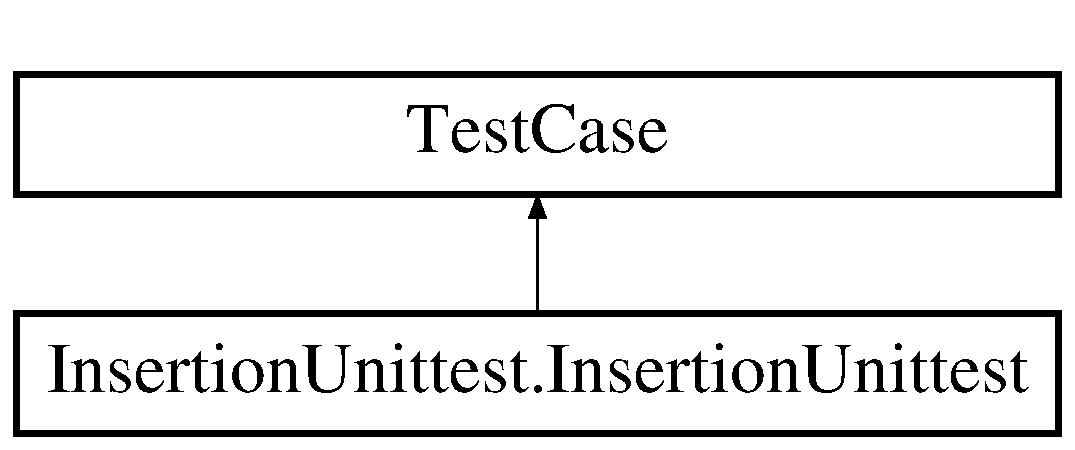
\includegraphics[height=2.000000cm]{classInsertionUnittest_1_1InsertionUnittest}
\end{center}
\end{figure}
\subsection*{Public Member Functions}
\begin{DoxyCompactItemize}
\item 
\hypertarget{classInsertionUnittest_1_1InsertionUnittest_a0e924dce2a16e67553892ba3b9c38f20}{def {\bfseries set\-Up}}\label{classInsertionUnittest_1_1InsertionUnittest_a0e924dce2a16e67553892ba3b9c38f20}

\item 
\hypertarget{classInsertionUnittest_1_1InsertionUnittest_ac59fb29a65050c957445771b0e09d119}{def {\bfseries test\-Tables}}\label{classInsertionUnittest_1_1InsertionUnittest_ac59fb29a65050c957445771b0e09d119}

\item 
\hypertarget{classInsertionUnittest_1_1InsertionUnittest_a0d0c53a8b26a73e96295c0aae0da3bf7}{def {\bfseries test\-R\-N\-A}}\label{classInsertionUnittest_1_1InsertionUnittest_a0d0c53a8b26a73e96295c0aae0da3bf7}

\item 
\hypertarget{classInsertionUnittest_1_1InsertionUnittest_a6dc5f5841035d1123d84971ec64f0082}{def {\bfseries test\-R\-N\-A\-X\-Refs}}\label{classInsertionUnittest_1_1InsertionUnittest_a6dc5f5841035d1123d84971ec64f0082}

\item 
\hypertarget{classInsertionUnittest_1_1InsertionUnittest_ac388b39222c76b282b4861068f8ccb5b}{def {\bfseries test\-P\-R\-I\-Cat\-R\-A\-P\-I\-D}}\label{classInsertionUnittest_1_1InsertionUnittest_ac388b39222c76b282b4861068f8ccb5b}

\item 
\hypertarget{classInsertionUnittest_1_1InsertionUnittest_a0627c10235aa1952160a68ef59e71fe4}{def {\bfseries test\-Interacting\-Cat\-R\-A\-P\-I\-D}}\label{classInsertionUnittest_1_1InsertionUnittest_a0627c10235aa1952160a68ef59e71fe4}

\item 
\hypertarget{classInsertionUnittest_1_1InsertionUnittest_a4591b7b11d32082884753a91df28e7e9}{def {\bfseries test\-R\-N\-A\-Tissue\-Expression}}\label{classInsertionUnittest_1_1InsertionUnittest_a4591b7b11d32082884753a91df28e7e9}

\item 
\hypertarget{classInsertionUnittest_1_1InsertionUnittest_ac9ff2af4f41e62e010c746aca15253db}{def {\bfseries tear\-Down}}\label{classInsertionUnittest_1_1InsertionUnittest_ac9ff2af4f41e62e010c746aca15253db}

\end{DoxyCompactItemize}
\subsection*{Public Attributes}
\begin{DoxyCompactItemize}
\item 
\hypertarget{classInsertionUnittest_1_1InsertionUnittest_af17b4ac18e71a7333ab24dec3ff31fe9}{{\bfseries D\-B\-Path}}\label{classInsertionUnittest_1_1InsertionUnittest_af17b4ac18e71a7333ab24dec3ff31fe9}

\item 
\hypertarget{classInsertionUnittest_1_1InsertionUnittest_ac2018da9708216f10f7c002425b47bc3}{{\bfseries sql\-\_\-session}}\label{classInsertionUnittest_1_1InsertionUnittest_ac2018da9708216f10f7c002425b47bc3}

\item 
\hypertarget{classInsertionUnittest_1_1InsertionUnittest_a25a2a9b1cb4c24737ba123dd01f22744}{{\bfseries db\-\_\-engine}}\label{classInsertionUnittest_1_1InsertionUnittest_a25a2a9b1cb4c24737ba123dd01f22744}

\end{DoxyCompactItemize}


The documentation for this class was generated from the following file\-:\begin{DoxyCompactItemize}
\item 
test/fr/tagc/rainet/core/Insertion\-Unittest.\-py\end{DoxyCompactItemize}

\hypertarget{classsrc_1_1fr_1_1tagc_1_1rainet_1_1core_1_1data_1_1InteractingProtein_1_1InteractingProtein}{\section{src.\-fr.\-tagc.\-rainet.\-core.\-data.\-Interacting\-Protein.\-Interacting\-Protein Class Reference}
\label{classsrc_1_1fr_1_1tagc_1_1rainet_1_1core_1_1data_1_1InteractingProtein_1_1InteractingProtein}\index{src.\-fr.\-tagc.\-rainet.\-core.\-data.\-Interacting\-Protein.\-Interacting\-Protein@{src.\-fr.\-tagc.\-rainet.\-core.\-data.\-Interacting\-Protein.\-Interacting\-Protein}}
}
Inheritance diagram for src.\-fr.\-tagc.\-rainet.\-core.\-data.\-Interacting\-Protein.\-Interacting\-Protein\-:\begin{figure}[H]
\begin{center}
\leavevmode
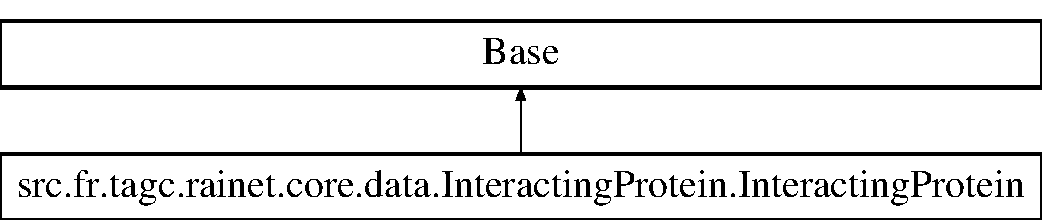
\includegraphics[height=2.000000cm]{classsrc_1_1fr_1_1tagc_1_1rainet_1_1core_1_1data_1_1InteractingProtein_1_1InteractingProtein}
\end{center}
\end{figure}
\subsection*{Public Member Functions}
\begin{DoxyCompactItemize}
\item 
\hypertarget{classsrc_1_1fr_1_1tagc_1_1rainet_1_1core_1_1data_1_1InteractingProtein_1_1InteractingProtein_a8b8919e52da2bdae7352d25902286d30}{def {\bfseries \-\_\-\-\_\-init\-\_\-\-\_\-}}\label{classsrc_1_1fr_1_1tagc_1_1rainet_1_1core_1_1data_1_1InteractingProtein_1_1InteractingProtein_a8b8919e52da2bdae7352d25902286d30}

\item 
\hypertarget{classsrc_1_1fr_1_1tagc_1_1rainet_1_1core_1_1data_1_1InteractingProtein_1_1InteractingProtein_a8e522e5e5371f020db5afc846da20071}{def \hyperlink{classsrc_1_1fr_1_1tagc_1_1rainet_1_1core_1_1data_1_1InteractingProtein_1_1InteractingProtein_a8e522e5e5371f020db5afc846da20071}{add\-\_\-to\-\_\-session}}\label{classsrc_1_1fr_1_1tagc_1_1rainet_1_1core_1_1data_1_1InteractingProtein_1_1InteractingProtein_a8e522e5e5371f020db5afc846da20071}

\begin{DoxyCompactList}\small\item\em Add the object to S\-Q\-L\-Alchemy session if it is linked to a protein. \end{DoxyCompactList}\end{DoxyCompactItemize}
\subsection*{Public Attributes}
\begin{DoxyCompactItemize}
\item 
\hypertarget{classsrc_1_1fr_1_1tagc_1_1rainet_1_1core_1_1data_1_1InteractingProtein_1_1InteractingProtein_af6e40087a910a5e1daf8b55c2e07b987}{{\bfseries uniprot\-A\-C}}\label{classsrc_1_1fr_1_1tagc_1_1rainet_1_1core_1_1data_1_1InteractingProtein_1_1InteractingProtein_af6e40087a910a5e1daf8b55c2e07b987}

\end{DoxyCompactItemize}
\subsection*{Static Public Attributes}
\begin{DoxyCompactItemize}
\item 
\hypertarget{classsrc_1_1fr_1_1tagc_1_1rainet_1_1core_1_1data_1_1InteractingProtein_1_1InteractingProtein_a63ff91371a3e6c44631bfb46f42e84c7}{tuple {\bfseries uniprot\-A\-C} = Column( String, Foreign\-Key('Protein.\-uniprot\-A\-C'), primary\-\_\-key=True)}\label{classsrc_1_1fr_1_1tagc_1_1rainet_1_1core_1_1data_1_1InteractingProtein_1_1InteractingProtein_a63ff91371a3e6c44631bfb46f42e84c7}

\end{DoxyCompactItemize}


The documentation for this class was generated from the following file\-:\begin{DoxyCompactItemize}
\item 
src/fr/tagc/rainet/core/data/Interacting\-Protein.\-py\end{DoxyCompactItemize}

\hypertarget{classsrc_1_1fr_1_1tagc_1_1rainet_1_1core_1_1data_1_1InteractingRNA_1_1InteractingRNA}{\section{src.\-fr.\-tagc.\-rainet.\-core.\-data.\-Interacting\-R\-N\-A.\-Interacting\-R\-N\-A Class Reference}
\label{classsrc_1_1fr_1_1tagc_1_1rainet_1_1core_1_1data_1_1InteractingRNA_1_1InteractingRNA}\index{src.\-fr.\-tagc.\-rainet.\-core.\-data.\-Interacting\-R\-N\-A.\-Interacting\-R\-N\-A@{src.\-fr.\-tagc.\-rainet.\-core.\-data.\-Interacting\-R\-N\-A.\-Interacting\-R\-N\-A}}
}
Inheritance diagram for src.\-fr.\-tagc.\-rainet.\-core.\-data.\-Interacting\-R\-N\-A.\-Interacting\-R\-N\-A\-:\begin{figure}[H]
\begin{center}
\leavevmode
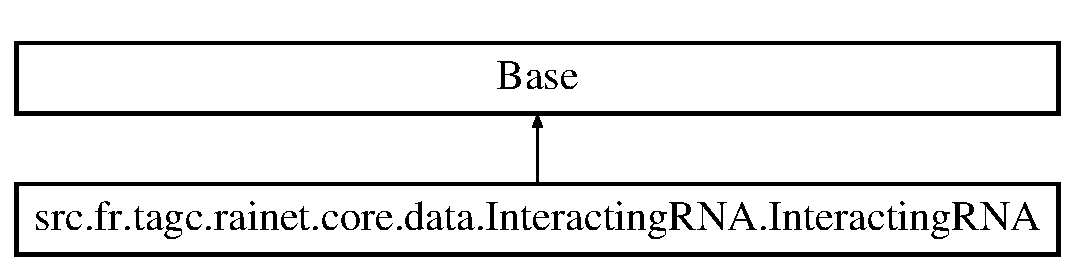
\includegraphics[height=2.000000cm]{classsrc_1_1fr_1_1tagc_1_1rainet_1_1core_1_1data_1_1InteractingRNA_1_1InteractingRNA}
\end{center}
\end{figure}
\subsection*{Public Member Functions}
\begin{DoxyCompactItemize}
\item 
\hypertarget{classsrc_1_1fr_1_1tagc_1_1rainet_1_1core_1_1data_1_1InteractingRNA_1_1InteractingRNA_a086d9a23e2d560554a345a53bae0b18f}{def {\bfseries \-\_\-\-\_\-init\-\_\-\-\_\-}}\label{classsrc_1_1fr_1_1tagc_1_1rainet_1_1core_1_1data_1_1InteractingRNA_1_1InteractingRNA_a086d9a23e2d560554a345a53bae0b18f}

\item 
\hypertarget{classsrc_1_1fr_1_1tagc_1_1rainet_1_1core_1_1data_1_1InteractingRNA_1_1InteractingRNA_a9d14d77bb37ed9fd7f72746eedc57528}{def \hyperlink{classsrc_1_1fr_1_1tagc_1_1rainet_1_1core_1_1data_1_1InteractingRNA_1_1InteractingRNA_a9d14d77bb37ed9fd7f72746eedc57528}{add\-\_\-to\-\_\-session}}\label{classsrc_1_1fr_1_1tagc_1_1rainet_1_1core_1_1data_1_1InteractingRNA_1_1InteractingRNA_a9d14d77bb37ed9fd7f72746eedc57528}

\begin{DoxyCompactList}\small\item\em Add the object to S\-Q\-L\-Alchemy session if it is linked to a protein. \end{DoxyCompactList}\end{DoxyCompactItemize}
\subsection*{Public Attributes}
\begin{DoxyCompactItemize}
\item 
\hypertarget{classsrc_1_1fr_1_1tagc_1_1rainet_1_1core_1_1data_1_1InteractingRNA_1_1InteractingRNA_ae1d8c65a8e43e46648ce6f3a1c977752}{{\bfseries transcript\-I\-D}}\label{classsrc_1_1fr_1_1tagc_1_1rainet_1_1core_1_1data_1_1InteractingRNA_1_1InteractingRNA_ae1d8c65a8e43e46648ce6f3a1c977752}

\end{DoxyCompactItemize}
\subsection*{Static Public Attributes}
\begin{DoxyCompactItemize}
\item 
\hypertarget{classsrc_1_1fr_1_1tagc_1_1rainet_1_1core_1_1data_1_1InteractingRNA_1_1InteractingRNA_af6eb5c1cb3bc037cf4a68e4d4e33fe06}{tuple {\bfseries transcript\-I\-D} = Column( String, Foreign\-Key('R\-N\-A.\-transcript\-I\-D'), primary\-\_\-key=True)}\label{classsrc_1_1fr_1_1tagc_1_1rainet_1_1core_1_1data_1_1InteractingRNA_1_1InteractingRNA_af6eb5c1cb3bc037cf4a68e4d4e33fe06}

\end{DoxyCompactItemize}


The documentation for this class was generated from the following file\-:\begin{DoxyCompactItemize}
\item 
src/fr/tagc/rainet/core/data/Interacting\-R\-N\-A.\-py\end{DoxyCompactItemize}

\hypertarget{classsrc_1_1fr_1_1tagc_1_1rainet_1_1core_1_1execution_1_1InteractiveQueryStrategy_1_1InteractiveQueryStrategy}{\section{src.\-fr.\-tagc.\-rainet.\-core.\-execution.\-Interactive\-Query\-Strategy.\-Interactive\-Query\-Strategy Class Reference}
\label{classsrc_1_1fr_1_1tagc_1_1rainet_1_1core_1_1execution_1_1InteractiveQueryStrategy_1_1InteractiveQueryStrategy}\index{src.\-fr.\-tagc.\-rainet.\-core.\-execution.\-Interactive\-Query\-Strategy.\-Interactive\-Query\-Strategy@{src.\-fr.\-tagc.\-rainet.\-core.\-execution.\-Interactive\-Query\-Strategy.\-Interactive\-Query\-Strategy}}
}
Inheritance diagram for src.\-fr.\-tagc.\-rainet.\-core.\-execution.\-Interactive\-Query\-Strategy.\-Interactive\-Query\-Strategy\-:\begin{figure}[H]
\begin{center}
\leavevmode
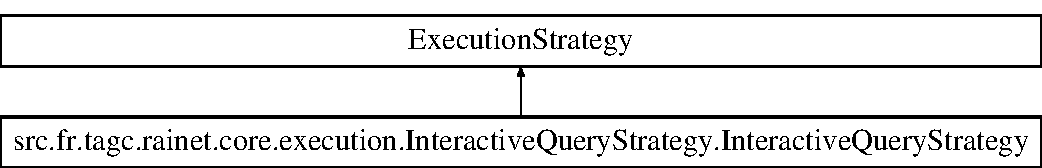
\includegraphics[height=2.000000cm]{classsrc_1_1fr_1_1tagc_1_1rainet_1_1core_1_1execution_1_1InteractiveQueryStrategy_1_1InteractiveQueryStrategy}
\end{center}
\end{figure}
\subsection*{Public Member Functions}
\begin{DoxyCompactItemize}
\item 
\hypertarget{classsrc_1_1fr_1_1tagc_1_1rainet_1_1core_1_1execution_1_1InteractiveQueryStrategy_1_1InteractiveQueryStrategy_a73f1b99c14678d69dd25f928847713f8}{def {\bfseries execute}}\label{classsrc_1_1fr_1_1tagc_1_1rainet_1_1core_1_1execution_1_1InteractiveQueryStrategy_1_1InteractiveQueryStrategy_a73f1b99c14678d69dd25f928847713f8}

\item 
\hypertarget{classsrc_1_1fr_1_1tagc_1_1rainet_1_1core_1_1execution_1_1InteractiveQueryStrategy_1_1InteractiveQueryStrategy_ab2280873902881360927f2a66d81e8ce}{def {\bfseries read\-\_\-query}}\label{classsrc_1_1fr_1_1tagc_1_1rainet_1_1core_1_1execution_1_1InteractiveQueryStrategy_1_1InteractiveQueryStrategy_ab2280873902881360927f2a66d81e8ce}

\item 
\hypertarget{classsrc_1_1fr_1_1tagc_1_1rainet_1_1core_1_1execution_1_1InteractiveQueryStrategy_1_1InteractiveQueryStrategy_af4c5794a2795aa7dc70f87d51e303404}{def {\bfseries perform\-\_\-query}}\label{classsrc_1_1fr_1_1tagc_1_1rainet_1_1core_1_1execution_1_1InteractiveQueryStrategy_1_1InteractiveQueryStrategy_af4c5794a2795aa7dc70f87d51e303404}

\item 
\hypertarget{classsrc_1_1fr_1_1tagc_1_1rainet_1_1core_1_1execution_1_1InteractiveQueryStrategy_1_1InteractiveQueryStrategy_aaf4fa0321ef28d630612f5008466fa1e}{def {\bfseries export\-\_\-query\-\_\-result}}\label{classsrc_1_1fr_1_1tagc_1_1rainet_1_1core_1_1execution_1_1InteractiveQueryStrategy_1_1InteractiveQueryStrategy_aaf4fa0321ef28d630612f5008466fa1e}

\end{DoxyCompactItemize}
\subsection*{Public Attributes}
\begin{DoxyCompactItemize}
\item 
\hypertarget{classsrc_1_1fr_1_1tagc_1_1rainet_1_1core_1_1execution_1_1InteractiveQueryStrategy_1_1InteractiveQueryStrategy_a7e0668a24218ccbb4812c629aa382516}{{\bfseries D\-B\-Path}}\label{classsrc_1_1fr_1_1tagc_1_1rainet_1_1core_1_1execution_1_1InteractiveQueryStrategy_1_1InteractiveQueryStrategy_a7e0668a24218ccbb4812c629aa382516}

\end{DoxyCompactItemize}


The documentation for this class was generated from the following file\-:\begin{DoxyCompactItemize}
\item 
src/fr/tagc/rainet/core/execution/Interactive\-Query\-Strategy.\-py\end{DoxyCompactItemize}

\hypertarget{classsrc_1_1core_1_1util_1_1tools_1_1Iupred_1_1Iupred}{\section{src.\-core.\-util.\-tools.\-Iupred.\-Iupred Class Reference}
\label{classsrc_1_1core_1_1util_1_1tools_1_1Iupred_1_1Iupred}\index{src.\-core.\-util.\-tools.\-Iupred.\-Iupred@{src.\-core.\-util.\-tools.\-Iupred.\-Iupred}}
}
\subsection*{Public Member Functions}
\begin{DoxyCompactItemize}
\item 
\hypertarget{classsrc_1_1core_1_1util_1_1tools_1_1Iupred_1_1Iupred_aa97a1c7fdb4d71aabf21b991b2bb776a}{def {\bfseries \-\_\-\-\_\-init\-\_\-\-\_\-}}\label{classsrc_1_1core_1_1util_1_1tools_1_1Iupred_1_1Iupred_aa97a1c7fdb4d71aabf21b991b2bb776a}

\item 
\hypertarget{classsrc_1_1core_1_1util_1_1tools_1_1Iupred_1_1Iupred_a926970f11daa2e22bac028681d406aa7}{def {\bfseries iupred\-\_\-analysis}}\label{classsrc_1_1core_1_1util_1_1tools_1_1Iupred_1_1Iupred_a926970f11daa2e22bac028681d406aa7}

\end{DoxyCompactItemize}
\subsection*{Static Public Member Functions}
\begin{DoxyCompactItemize}
\item 
\hypertarget{classsrc_1_1core_1_1util_1_1tools_1_1Iupred_1_1Iupred_ab44cc4f1500c7a512036ff757aa33c41}{def {\bfseries global\-\_\-iupred\-\_\-analysis}}\label{classsrc_1_1core_1_1util_1_1tools_1_1Iupred_1_1Iupred_ab44cc4f1500c7a512036ff757aa33c41}

\item 
\hypertarget{classsrc_1_1core_1_1util_1_1tools_1_1Iupred_1_1Iupred_a5648fd4ecb62f1c0be233d2db41fac6d}{def {\bfseries iupred\-\_\-info}}\label{classsrc_1_1core_1_1util_1_1tools_1_1Iupred_1_1Iupred_a5648fd4ecb62f1c0be233d2db41fac6d}

\item 
\hypertarget{classsrc_1_1core_1_1util_1_1tools_1_1Iupred_1_1Iupred_a3b51420992f771cdc8a42d4c75fd61af}{def {\bfseries iupred\-\_\-string\-\_\-info}}\label{classsrc_1_1core_1_1util_1_1tools_1_1Iupred_1_1Iupred_a3b51420992f771cdc8a42d4c75fd61af}

\item 
\hypertarget{classsrc_1_1core_1_1util_1_1tools_1_1Iupred_1_1Iupred_ae375b5b15f3ad45d5de0c91de614a5c8}{def {\bfseries make\-\_\-iupred\-\_\-file}}\label{classsrc_1_1core_1_1util_1_1tools_1_1Iupred_1_1Iupred_ae375b5b15f3ad45d5de0c91de614a5c8}

\end{DoxyCompactItemize}
\subsection*{Public Attributes}
\begin{DoxyCompactItemize}
\item 
\hypertarget{classsrc_1_1core_1_1util_1_1tools_1_1Iupred_1_1Iupred_a2b4d26412ad9a84336800751ce49adb0}{{\bfseries path\-\_\-output}}\label{classsrc_1_1core_1_1util_1_1tools_1_1Iupred_1_1Iupred_a2b4d26412ad9a84336800751ce49adb0}

\item 
\hypertarget{classsrc_1_1core_1_1util_1_1tools_1_1Iupred_1_1Iupred_adf0b98b5d9c54aa5cf1ea28d471c1147}{{\bfseries iupred\-\_\-path}}\label{classsrc_1_1core_1_1util_1_1tools_1_1Iupred_1_1Iupred_adf0b98b5d9c54aa5cf1ea28d471c1147}

\item 
\hypertarget{classsrc_1_1core_1_1util_1_1tools_1_1Iupred_1_1Iupred_a6ebe0afbd3972992a7dedc5975c809c5}{{\bfseries fastafile}}\label{classsrc_1_1core_1_1util_1_1tools_1_1Iupred_1_1Iupred_a6ebe0afbd3972992a7dedc5975c809c5}

\item 
\hypertarget{classsrc_1_1core_1_1util_1_1tools_1_1Iupred_1_1Iupred_ae64604e778dd1e3ba3ef140360da5cdb}{{\bfseries prot}}\label{classsrc_1_1core_1_1util_1_1tools_1_1Iupred_1_1Iupred_ae64604e778dd1e3ba3ef140360da5cdb}

\end{DoxyCompactItemize}


The documentation for this class was generated from the following file\-:\begin{DoxyCompactItemize}
\item 
rbp-\/motif/src/core/util/tools/Iupred.\-py\end{DoxyCompactItemize}

\hypertarget{classsrc_1_1fr_1_1tagc_1_1rainet_1_1core_1_1util_1_1subprocess_1_1JobPoolerFolder_1_1JobPoolerFolder}{\section{src.\-fr.\-tagc.\-rainet.\-core.\-util.\-subprocess.\-Job\-Pooler\-Folder.\-Job\-Pooler\-Folder Class Reference}
\label{classsrc_1_1fr_1_1tagc_1_1rainet_1_1core_1_1util_1_1subprocess_1_1JobPoolerFolder_1_1JobPoolerFolder}\index{src.\-fr.\-tagc.\-rainet.\-core.\-util.\-subprocess.\-Job\-Pooler\-Folder.\-Job\-Pooler\-Folder@{src.\-fr.\-tagc.\-rainet.\-core.\-util.\-subprocess.\-Job\-Pooler\-Folder.\-Job\-Pooler\-Folder}}
}
Inheritance diagram for src.\-fr.\-tagc.\-rainet.\-core.\-util.\-subprocess.\-Job\-Pooler\-Folder.\-Job\-Pooler\-Folder\-:\begin{figure}[H]
\begin{center}
\leavevmode
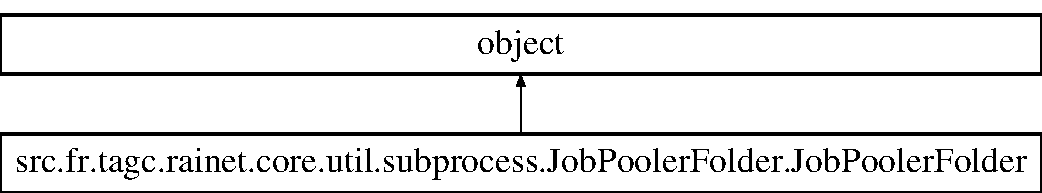
\includegraphics[height=2.000000cm]{classsrc_1_1fr_1_1tagc_1_1rainet_1_1core_1_1util_1_1subprocess_1_1JobPoolerFolder_1_1JobPoolerFolder}
\end{center}
\end{figure}
\subsection*{Public Member Functions}
\begin{DoxyCompactItemize}
\item 
\hypertarget{classsrc_1_1fr_1_1tagc_1_1rainet_1_1core_1_1util_1_1subprocess_1_1JobPoolerFolder_1_1JobPoolerFolder_a94d3a43af26d648489605ab7a05e9602}{def {\bfseries \-\_\-\-\_\-init\-\_\-\-\_\-}}\label{classsrc_1_1fr_1_1tagc_1_1rainet_1_1core_1_1util_1_1subprocess_1_1JobPoolerFolder_1_1JobPoolerFolder_a94d3a43af26d648489605ab7a05e9602}

\item 
\hypertarget{classsrc_1_1fr_1_1tagc_1_1rainet_1_1core_1_1util_1_1subprocess_1_1JobPoolerFolder_1_1JobPoolerFolder_ad31bdc5a80a8e6fb33c3e9c33c9b0564}{def {\bfseries parallel}}\label{classsrc_1_1fr_1_1tagc_1_1rainet_1_1core_1_1util_1_1subprocess_1_1JobPoolerFolder_1_1JobPoolerFolder_ad31bdc5a80a8e6fb33c3e9c33c9b0564}

\end{DoxyCompactItemize}
\subsection*{Public Attributes}
\begin{DoxyCompactItemize}
\item 
\hypertarget{classsrc_1_1fr_1_1tagc_1_1rainet_1_1core_1_1util_1_1subprocess_1_1JobPoolerFolder_1_1JobPoolerFolder_a09a5abc8e78560dda7f866e0ab3025b1}{{\bfseries input\-Folder}}\label{classsrc_1_1fr_1_1tagc_1_1rainet_1_1core_1_1util_1_1subprocess_1_1JobPoolerFolder_1_1JobPoolerFolder_a09a5abc8e78560dda7f866e0ab3025b1}

\item 
\hypertarget{classsrc_1_1fr_1_1tagc_1_1rainet_1_1core_1_1util_1_1subprocess_1_1JobPoolerFolder_1_1JobPoolerFolder_a1effb681768d567a895cbfd76f79bd23}{{\bfseries command\-String}}\label{classsrc_1_1fr_1_1tagc_1_1rainet_1_1core_1_1util_1_1subprocess_1_1JobPoolerFolder_1_1JobPoolerFolder_a1effb681768d567a895cbfd76f79bd23}

\item 
\hypertarget{classsrc_1_1fr_1_1tagc_1_1rainet_1_1core_1_1util_1_1subprocess_1_1JobPoolerFolder_1_1JobPoolerFolder_a842b71dce3d982f8d87a89381025559f}{{\bfseries num\-Threads}}\label{classsrc_1_1fr_1_1tagc_1_1rainet_1_1core_1_1util_1_1subprocess_1_1JobPoolerFolder_1_1JobPoolerFolder_a842b71dce3d982f8d87a89381025559f}

\item 
\hypertarget{classsrc_1_1fr_1_1tagc_1_1rainet_1_1core_1_1util_1_1subprocess_1_1JobPoolerFolder_1_1JobPoolerFolder_a778e7aa392237232731f9f14244b5d5c}{{\bfseries sleep\-Time}}\label{classsrc_1_1fr_1_1tagc_1_1rainet_1_1core_1_1util_1_1subprocess_1_1JobPoolerFolder_1_1JobPoolerFolder_a778e7aa392237232731f9f14244b5d5c}

\end{DoxyCompactItemize}


The documentation for this class was generated from the following file\-:\begin{DoxyCompactItemize}
\item 
src/fr/tagc/rainet/core/util/subprocess/Job\-Pooler\-Folder.\-py\end{DoxyCompactItemize}

\hypertarget{classsrc_1_1fr_1_1tagc_1_1rainet_1_1core_1_1data_1_1KEGGPathway_1_1KEGGPathway}{\section{src.\-fr.\-tagc.\-rainet.\-core.\-data.\-K\-E\-G\-G\-Pathway.\-K\-E\-G\-G\-Pathway Class Reference}
\label{classsrc_1_1fr_1_1tagc_1_1rainet_1_1core_1_1data_1_1KEGGPathway_1_1KEGGPathway}\index{src.\-fr.\-tagc.\-rainet.\-core.\-data.\-K\-E\-G\-G\-Pathway.\-K\-E\-G\-G\-Pathway@{src.\-fr.\-tagc.\-rainet.\-core.\-data.\-K\-E\-G\-G\-Pathway.\-K\-E\-G\-G\-Pathway}}
}
Inheritance diagram for src.\-fr.\-tagc.\-rainet.\-core.\-data.\-K\-E\-G\-G\-Pathway.\-K\-E\-G\-G\-Pathway\-:\begin{figure}[H]
\begin{center}
\leavevmode
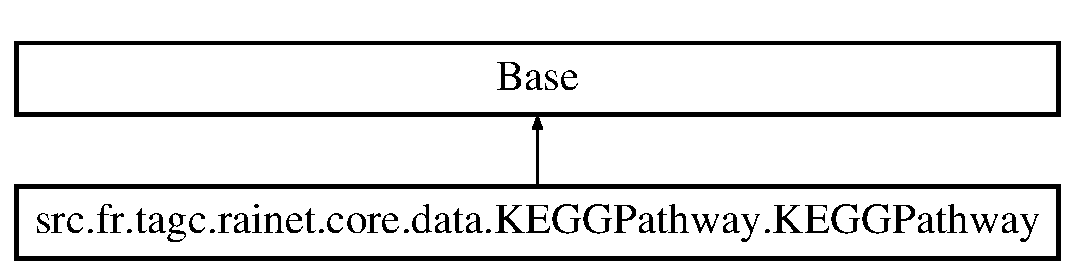
\includegraphics[height=2.000000cm]{classsrc_1_1fr_1_1tagc_1_1rainet_1_1core_1_1data_1_1KEGGPathway_1_1KEGGPathway}
\end{center}
\end{figure}
\subsection*{Public Member Functions}
\begin{DoxyCompactItemize}
\item 
\hypertarget{classsrc_1_1fr_1_1tagc_1_1rainet_1_1core_1_1data_1_1KEGGPathway_1_1KEGGPathway_aebfe3b1e5b19192e4c587beee14c50f1}{def {\bfseries \-\_\-\-\_\-init\-\_\-\-\_\-}}\label{classsrc_1_1fr_1_1tagc_1_1rainet_1_1core_1_1data_1_1KEGGPathway_1_1KEGGPathway_aebfe3b1e5b19192e4c587beee14c50f1}

\item 
\hypertarget{classsrc_1_1fr_1_1tagc_1_1rainet_1_1core_1_1data_1_1KEGGPathway_1_1KEGGPathway_a569d7ef8d58fd928a53ba69b3360d332}{def \hyperlink{classsrc_1_1fr_1_1tagc_1_1rainet_1_1core_1_1data_1_1KEGGPathway_1_1KEGGPathway_a569d7ef8d58fd928a53ba69b3360d332}{add\-\_\-to\-\_\-session}}\label{classsrc_1_1fr_1_1tagc_1_1rainet_1_1core_1_1data_1_1KEGGPathway_1_1KEGGPathway_a569d7ef8d58fd928a53ba69b3360d332}

\begin{DoxyCompactList}\small\item\em Add the object to S\-Q\-L\-Alchemy session if it is linked to a protein. \end{DoxyCompactList}\item 
\hypertarget{classsrc_1_1fr_1_1tagc_1_1rainet_1_1core_1_1data_1_1KEGGPathway_1_1KEGGPathway_ab9820b7b31e392e1c4e7937dd0c1e9d1}{def \hyperlink{classsrc_1_1fr_1_1tagc_1_1rainet_1_1core_1_1data_1_1KEGGPathway_1_1KEGGPathway_ab9820b7b31e392e1c4e7937dd0c1e9d1}{add\-\_\-annotated\-\_\-protein}}\label{classsrc_1_1fr_1_1tagc_1_1rainet_1_1core_1_1data_1_1KEGGPathway_1_1KEGGPathway_ab9820b7b31e392e1c4e7937dd0c1e9d1}

\begin{DoxyCompactList}\small\item\em Add an annotated protein to the list. \end{DoxyCompactList}\end{DoxyCompactItemize}
\subsection*{Public Attributes}
\begin{DoxyCompactItemize}
\item 
\hypertarget{classsrc_1_1fr_1_1tagc_1_1rainet_1_1core_1_1data_1_1KEGGPathway_1_1KEGGPathway_af91ad118d445204630ce0a5375ea80fc}{{\bfseries kegg\-I\-D}}\label{classsrc_1_1fr_1_1tagc_1_1rainet_1_1core_1_1data_1_1KEGGPathway_1_1KEGGPathway_af91ad118d445204630ce0a5375ea80fc}

\item 
\hypertarget{classsrc_1_1fr_1_1tagc_1_1rainet_1_1core_1_1data_1_1KEGGPathway_1_1KEGGPathway_a0eab1a22463bd1429b70856918d9be87}{{\bfseries kegg\-Name}}\label{classsrc_1_1fr_1_1tagc_1_1rainet_1_1core_1_1data_1_1KEGGPathway_1_1KEGGPathway_a0eab1a22463bd1429b70856918d9be87}

\end{DoxyCompactItemize}
\subsection*{Static Public Attributes}
\begin{DoxyCompactItemize}
\item 
\hypertarget{classsrc_1_1fr_1_1tagc_1_1rainet_1_1core_1_1data_1_1KEGGPathway_1_1KEGGPathway_a87bfa8948cee850036a02dc04a97f3e3}{tuple {\bfseries kegg\-I\-D} = Column( String, primary\-\_\-key = True )}\label{classsrc_1_1fr_1_1tagc_1_1rainet_1_1core_1_1data_1_1KEGGPathway_1_1KEGGPathway_a87bfa8948cee850036a02dc04a97f3e3}

\item 
\hypertarget{classsrc_1_1fr_1_1tagc_1_1rainet_1_1core_1_1data_1_1KEGGPathway_1_1KEGGPathway_a376c34777443e3b323cbffacbf0b3c97}{tuple {\bfseries kegg\-Name} = Column( String )}\label{classsrc_1_1fr_1_1tagc_1_1rainet_1_1core_1_1data_1_1KEGGPathway_1_1KEGGPathway_a376c34777443e3b323cbffacbf0b3c97}

\item 
\hypertarget{classsrc_1_1fr_1_1tagc_1_1rainet_1_1core_1_1data_1_1KEGGPathway_1_1KEGGPathway_aa7e0d488e23045e0c308414e819c0648}{tuple {\bfseries annotated\-Proteins} = relationship('Protein', secondary=Protein\-K\-E\-G\-G\-Annotation.\-\_\-\-\_\-table\-\_\-\-\_\-, backref=\char`\"{}kegg\-Annotations\char`\"{})}\label{classsrc_1_1fr_1_1tagc_1_1rainet_1_1core_1_1data_1_1KEGGPathway_1_1KEGGPathway_aa7e0d488e23045e0c308414e819c0648}

\end{DoxyCompactItemize}


The documentation for this class was generated from the following file\-:\begin{DoxyCompactItemize}
\item 
src/fr/tagc/rainet/core/data/K\-E\-G\-G\-Pathway.\-py\end{DoxyCompactItemize}

\hypertarget{classKnownScaffoldValidation_1_1KnownScaffoldValidation}{\section{Known\-Scaffold\-Validation.\-Known\-Scaffold\-Validation Class Reference}
\label{classKnownScaffoldValidation_1_1KnownScaffoldValidation}\index{Known\-Scaffold\-Validation.\-Known\-Scaffold\-Validation@{Known\-Scaffold\-Validation.\-Known\-Scaffold\-Validation}}
}
Inheritance diagram for Known\-Scaffold\-Validation.\-Known\-Scaffold\-Validation\-:\begin{figure}[H]
\begin{center}
\leavevmode
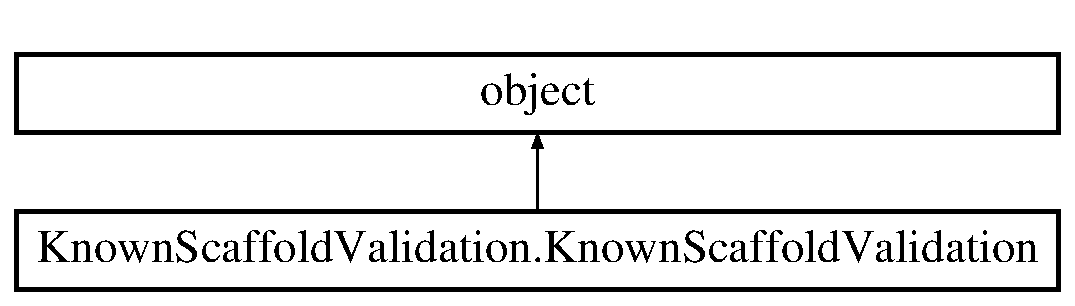
\includegraphics[height=2.000000cm]{classKnownScaffoldValidation_1_1KnownScaffoldValidation}
\end{center}
\end{figure}
\subsection*{Public Member Functions}
\begin{DoxyCompactItemize}
\item 
\hypertarget{classKnownScaffoldValidation_1_1KnownScaffoldValidation_a8208ea6ca4bf58be3de6b52e6fc2e534}{def {\bfseries \-\_\-\-\_\-init\-\_\-\-\_\-}}\label{classKnownScaffoldValidation_1_1KnownScaffoldValidation_a8208ea6ca4bf58be3de6b52e6fc2e534}

\item 
\hypertarget{classKnownScaffoldValidation_1_1KnownScaffoldValidation_a40a1f0303c948edf857b6e027c670dbe}{def {\bfseries read\-\_\-cat\-R\-A\-P\-I\-D\-\_\-file}}\label{classKnownScaffoldValidation_1_1KnownScaffoldValidation_a40a1f0303c948edf857b6e027c670dbe}

\item 
\hypertarget{classKnownScaffoldValidation_1_1KnownScaffoldValidation_a8902b56c40173ea2b8e44ec2a84c43f6}{def {\bfseries read\-\_\-\-N\-P\-Inter\-\_\-file}}\label{classKnownScaffoldValidation_1_1KnownScaffoldValidation_a8902b56c40173ea2b8e44ec2a84c43f6}

\item 
\hypertarget{classKnownScaffoldValidation_1_1KnownScaffoldValidation_aeea1918f29bee932d8aeab7f44e7a0b2}{def {\bfseries read\-\_\-manual\-\_\-list\-\_\-file}}\label{classKnownScaffoldValidation_1_1KnownScaffoldValidation_aeea1918f29bee932d8aeab7f44e7a0b2}

\item 
\hypertarget{classKnownScaffoldValidation_1_1KnownScaffoldValidation_ac472671daa0b785da6d6bfffdfc6571c}{def {\bfseries convert\-To\-Propensity}}\label{classKnownScaffoldValidation_1_1KnownScaffoldValidation_ac472671daa0b785da6d6bfffdfc6571c}

\end{DoxyCompactItemize}
\subsection*{Public Attributes}
\begin{DoxyCompactItemize}
\item 
\hypertarget{classKnownScaffoldValidation_1_1KnownScaffoldValidation_a081a627a2ed1df3939201e1d9aa5e0ae}{{\bfseries cat\-R\-A\-P\-I\-D\-File}}\label{classKnownScaffoldValidation_1_1KnownScaffoldValidation_a081a627a2ed1df3939201e1d9aa5e0ae}

\item 
\hypertarget{classKnownScaffoldValidation_1_1KnownScaffoldValidation_a03aa365fd9bb0714743db9533ce06cea}{{\bfseries validated\-File}}\label{classKnownScaffoldValidation_1_1KnownScaffoldValidation_a03aa365fd9bb0714743db9533ce06cea}

\item 
\hypertarget{classKnownScaffoldValidation_1_1KnownScaffoldValidation_a7f1629b328fdecfcd922175870401356}{{\bfseries wanted\-R\-N\-A\-File}}\label{classKnownScaffoldValidation_1_1KnownScaffoldValidation_a7f1629b328fdecfcd922175870401356}

\item 
\hypertarget{classKnownScaffoldValidation_1_1KnownScaffoldValidation_a9ff46a0491b20e9180a39e167c9d8f1c}{{\bfseries rainet\-D\-B}}\label{classKnownScaffoldValidation_1_1KnownScaffoldValidation_a9ff46a0491b20e9180a39e167c9d8f1c}

\item 
\hypertarget{classKnownScaffoldValidation_1_1KnownScaffoldValidation_ae3da82bc80918db72ce775de92f1bfe3}{{\bfseries output\-Folder}}\label{classKnownScaffoldValidation_1_1KnownScaffoldValidation_ae3da82bc80918db72ce775de92f1bfe3}

\item 
\hypertarget{classKnownScaffoldValidation_1_1KnownScaffoldValidation_a24c9f280adb1128418845a9b5cccc82e}{{\bfseries discriminative\-Power\-Cutoff}}\label{classKnownScaffoldValidation_1_1KnownScaffoldValidation_a24c9f280adb1128418845a9b5cccc82e}

\item 
\hypertarget{classKnownScaffoldValidation_1_1KnownScaffoldValidation_ad2d3aade2f7736899ddf6525c2d19a78}{{\bfseries zscore\-Cutoff}}\label{classKnownScaffoldValidation_1_1KnownScaffoldValidation_ad2d3aade2f7736899ddf6525c2d19a78}

\item 
\hypertarget{classKnownScaffoldValidation_1_1KnownScaffoldValidation_a17dfcda314e09ef666a5b53d03174f74}{{\bfseries top\-Proportion}}\label{classKnownScaffoldValidation_1_1KnownScaffoldValidation_a17dfcda314e09ef666a5b53d03174f74}

\item 
\hypertarget{classKnownScaffoldValidation_1_1KnownScaffoldValidation_a43400fdd8e6f6e003d524058a6ea8818}{{\bfseries npinter}}\label{classKnownScaffoldValidation_1_1KnownScaffoldValidation_a43400fdd8e6f6e003d524058a6ea8818}

\item 
\hypertarget{classKnownScaffoldValidation_1_1KnownScaffoldValidation_aefeef575f7e5fb0cb1c4b52124dd80af}{{\bfseries column\-For\-Plot}}\label{classKnownScaffoldValidation_1_1KnownScaffoldValidation_aefeef575f7e5fb0cb1c4b52124dd80af}

\item 
\hypertarget{classKnownScaffoldValidation_1_1KnownScaffoldValidation_aa663e5bccd18fe05f1e17564b2bbdf97}{{\bfseries search\-Space\-File}}\label{classKnownScaffoldValidation_1_1KnownScaffoldValidation_aa663e5bccd18fe05f1e17564b2bbdf97}

\item 
\hypertarget{classKnownScaffoldValidation_1_1KnownScaffoldValidation_ad38e2db3be76a32cdf926dff2b7b13c0}{{\bfseries zscore\-To\-Propensity}}\label{classKnownScaffoldValidation_1_1KnownScaffoldValidation_ad38e2db3be76a32cdf926dff2b7b13c0}

\item 
\hypertarget{classKnownScaffoldValidation_1_1KnownScaffoldValidation_ae1c59e48f79e46da6964ee181afc1473}{{\bfseries sql\-\_\-session}}\label{classKnownScaffoldValidation_1_1KnownScaffoldValidation_ae1c59e48f79e46da6964ee181afc1473}

\item 
\hypertarget{classKnownScaffoldValidation_1_1KnownScaffoldValidation_abedcfd494e77ee282d9373c9d088a042}{{\bfseries xref\-Dict}}\label{classKnownScaffoldValidation_1_1KnownScaffoldValidation_abedcfd494e77ee282d9373c9d088a042}

\end{DoxyCompactItemize}
\subsection*{Static Public Attributes}
\begin{DoxyCompactItemize}
\item 
\hypertarget{classKnownScaffoldValidation_1_1KnownScaffoldValidation_a4e4f98145aad840ab25a33b57f0cc1c3}{string {\bfseries S\-P\-E\-C\-I\-E\-S} = \char`\"{}Homo sapiens\char`\"{}}\label{classKnownScaffoldValidation_1_1KnownScaffoldValidation_a4e4f98145aad840ab25a33b57f0cc1c3}

\item 
\hypertarget{classKnownScaffoldValidation_1_1KnownScaffoldValidation_af0d8df4a1664ced28f9474a4645c50d6}{string {\bfseries M\-O\-L\-E\-C\-U\-L\-E\-B\-T\-Y\-P\-E} = \char`\"{}protein\char`\"{}}\label{classKnownScaffoldValidation_1_1KnownScaffoldValidation_af0d8df4a1664ced28f9474a4645c50d6}

\item 
\hypertarget{classKnownScaffoldValidation_1_1KnownScaffoldValidation_a53ea27a72aabd88609a9a57a5151373a}{string {\bfseries H\-Y\-P\-E\-R\-G\-E\-O\-M\-E\-T\-R\-I\-C\-\_\-\-T\-E\-S\-T\-\_\-\-S\-C\-R\-I\-P\-T} = \char`\"{}/home/diogo/workspace/tagc-\/rainet-\/R\-N\-A/src/fr/tagc/rainet/core/execution/processing/known\-Scaffold\-Examples/hypergeometric\-\_\-test.\-R\char`\"{}}\label{classKnownScaffoldValidation_1_1KnownScaffoldValidation_a53ea27a72aabd88609a9a57a5151373a}

\item 
\hypertarget{classKnownScaffoldValidation_1_1KnownScaffoldValidation_adbad4b16746163e28049d918f472a868}{string {\bfseries D\-I\-S\-T\-R\-I\-B\-U\-T\-I\-O\-N\-\_\-\-S\-C\-R\-I\-P\-T} = \char`\"{}/home/diogo/workspace/tagc-\/rainet-\/R\-N\-A/src/fr/tagc/rainet/core/execution/processing/known\-Scaffold\-Examples/plot\-\_\-distribution.\-R\char`\"{}}\label{classKnownScaffoldValidation_1_1KnownScaffoldValidation_adbad4b16746163e28049d918f472a868}

\item 
\hypertarget{classKnownScaffoldValidation_1_1KnownScaffoldValidation_a274e95bc24fff30e74160f4a74fefd75}{float {\bfseries C\-A\-T\-R\-A\-P\-I\-D\-\_\-\-Z\-S\-\_\-\-M\-E\-A\-N} = 23.\-25}\label{classKnownScaffoldValidation_1_1KnownScaffoldValidation_a274e95bc24fff30e74160f4a74fefd75}

\item 
\hypertarget{classKnownScaffoldValidation_1_1KnownScaffoldValidation_a4ce49b584e20575cbfc223857c09f6b6}{float {\bfseries C\-A\-T\-R\-A\-P\-I\-D\-\_\-\-Z\-S\-\_\-\-S\-T\-D} = 37.\-90}\label{classKnownScaffoldValidation_1_1KnownScaffoldValidation_a4ce49b584e20575cbfc223857c09f6b6}

\end{DoxyCompactItemize}


The documentation for this class was generated from the following file\-:\begin{DoxyCompactItemize}
\item 
src/fr/tagc/rainet/core/execution/processing/known\-Scaffold\-Examples/Known\-Scaffold\-Validation.\-py\end{DoxyCompactItemize}

\hypertarget{classsrc_1_1core_1_1util_1_1format_1_1LengthSeq_1_1LengthSeq}{\section{src.\-core.\-util.\-format.\-Length\-Seq.\-Length\-Seq Class Reference}
\label{classsrc_1_1core_1_1util_1_1format_1_1LengthSeq_1_1LengthSeq}\index{src.\-core.\-util.\-format.\-Length\-Seq.\-Length\-Seq@{src.\-core.\-util.\-format.\-Length\-Seq.\-Length\-Seq}}
}
\subsection*{Static Public Member Functions}
\begin{DoxyCompactItemize}
\item 
\hypertarget{classsrc_1_1core_1_1util_1_1format_1_1LengthSeq_1_1LengthSeq_a854767f4696701e7800d4df33a81440b}{def {\bfseries longest\-\_\-seq}}\label{classsrc_1_1core_1_1util_1_1format_1_1LengthSeq_1_1LengthSeq_a854767f4696701e7800d4df33a81440b}

\end{DoxyCompactItemize}


The documentation for this class was generated from the following file\-:\begin{DoxyCompactItemize}
\item 
rbp-\/motif/src/core/util/format/Length\-Seq.\-py\end{DoxyCompactItemize}

\hypertarget{classsrc_1_1fr_1_1tagc_1_1rainet_1_1core_1_1data_1_1LncRNA_1_1LncRNA}{\section{src.\-fr.\-tagc.\-rainet.\-core.\-data.\-Lnc\-R\-N\-A.\-Lnc\-R\-N\-A Class Reference}
\label{classsrc_1_1fr_1_1tagc_1_1rainet_1_1core_1_1data_1_1LncRNA_1_1LncRNA}\index{src.\-fr.\-tagc.\-rainet.\-core.\-data.\-Lnc\-R\-N\-A.\-Lnc\-R\-N\-A@{src.\-fr.\-tagc.\-rainet.\-core.\-data.\-Lnc\-R\-N\-A.\-Lnc\-R\-N\-A}}
}
Inheritance diagram for src.\-fr.\-tagc.\-rainet.\-core.\-data.\-Lnc\-R\-N\-A.\-Lnc\-R\-N\-A\-:\begin{figure}[H]
\begin{center}
\leavevmode
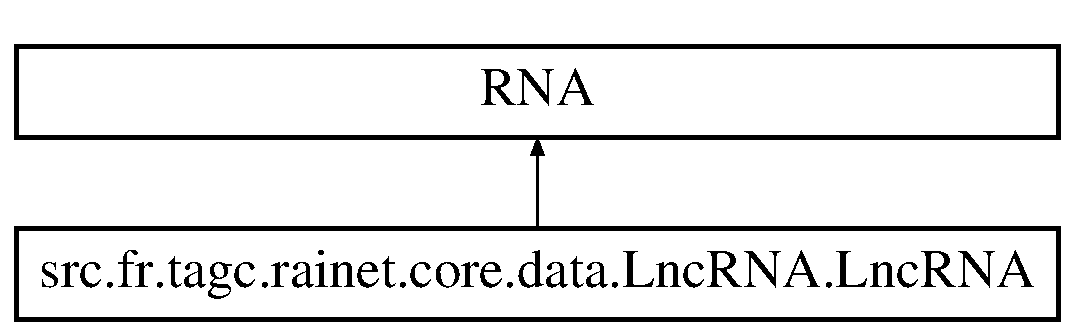
\includegraphics[height=2.000000cm]{classsrc_1_1fr_1_1tagc_1_1rainet_1_1core_1_1data_1_1LncRNA_1_1LncRNA}
\end{center}
\end{figure}
\subsection*{Public Member Functions}
\begin{DoxyCompactItemize}
\item 
\hypertarget{classsrc_1_1fr_1_1tagc_1_1rainet_1_1core_1_1data_1_1LncRNA_1_1LncRNA_a762274c557cd1facea9a63effe300ff1}{def {\bfseries \-\_\-\-\_\-init\-\_\-\-\_\-}}\label{classsrc_1_1fr_1_1tagc_1_1rainet_1_1core_1_1data_1_1LncRNA_1_1LncRNA_a762274c557cd1facea9a63effe300ff1}

\end{DoxyCompactItemize}
\subsection*{Static Public Attributes}
\begin{DoxyCompactItemize}
\item 
\hypertarget{classsrc_1_1fr_1_1tagc_1_1rainet_1_1core_1_1data_1_1LncRNA_1_1LncRNA_a2d3142d3b113878939c9edaf4cc92f94}{tuple {\bfseries transcript\-I\-D} = Column( String, Foreign\-Key('R\-N\-A.\-transcript\-I\-D'), primary\-\_\-key=True)}\label{classsrc_1_1fr_1_1tagc_1_1rainet_1_1core_1_1data_1_1LncRNA_1_1LncRNA_a2d3142d3b113878939c9edaf4cc92f94}

\end{DoxyCompactItemize}


The documentation for this class was generated from the following file\-:\begin{DoxyCompactItemize}
\item 
src/fr/tagc/rainet/core/data/Lnc\-R\-N\-A.\-py\end{DoxyCompactItemize}

\hypertarget{classsrc_1_1fr_1_1tagc_1_1rainet_1_1core_1_1execution_1_1analysis_1_1EnrichmentAnalysis_1_1LncRNe08e6e334d3ac6c2229a1d8a0df9192a}{\section{src.\-fr.\-tagc.\-rainet.\-core.\-execution.\-analysis.\-Enrichment\-Analysis.\-Lnc\-R\-N\-A\-Group\-Analysis.\-Lnc\-R\-N\-A\-Group\-Analysis Class Reference}
\label{classsrc_1_1fr_1_1tagc_1_1rainet_1_1core_1_1execution_1_1analysis_1_1EnrichmentAnalysis_1_1LncRNe08e6e334d3ac6c2229a1d8a0df9192a}\index{src.\-fr.\-tagc.\-rainet.\-core.\-execution.\-analysis.\-Enrichment\-Analysis.\-Lnc\-R\-N\-A\-Group\-Analysis.\-Lnc\-R\-N\-A\-Group\-Analysis@{src.\-fr.\-tagc.\-rainet.\-core.\-execution.\-analysis.\-Enrichment\-Analysis.\-Lnc\-R\-N\-A\-Group\-Analysis.\-Lnc\-R\-N\-A\-Group\-Analysis}}
}
Inheritance diagram for src.\-fr.\-tagc.\-rainet.\-core.\-execution.\-analysis.\-Enrichment\-Analysis.\-Lnc\-R\-N\-A\-Group\-Analysis.\-Lnc\-R\-N\-A\-Group\-Analysis\-:\begin{figure}[H]
\begin{center}
\leavevmode
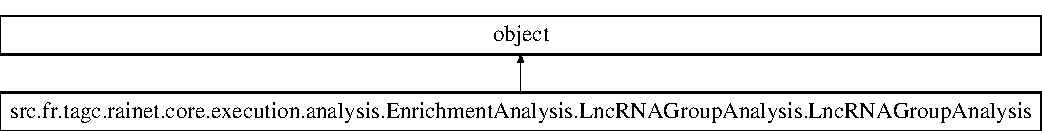
\includegraphics[height=1.761006cm]{classsrc_1_1fr_1_1tagc_1_1rainet_1_1core_1_1execution_1_1analysis_1_1EnrichmentAnalysis_1_1LncRNe08e6e334d3ac6c2229a1d8a0df9192a}
\end{center}
\end{figure}
\subsection*{Public Member Functions}
\begin{DoxyCompactItemize}
\item 
\hypertarget{classsrc_1_1fr_1_1tagc_1_1rainet_1_1core_1_1execution_1_1analysis_1_1EnrichmentAnalysis_1_1LncRNe08e6e334d3ac6c2229a1d8a0df9192a_ab1e25e4a5dc27a924d17848b8e813dc8}{def {\bfseries \-\_\-\-\_\-init\-\_\-\-\_\-}}\label{classsrc_1_1fr_1_1tagc_1_1rainet_1_1core_1_1execution_1_1analysis_1_1EnrichmentAnalysis_1_1LncRNe08e6e334d3ac6c2229a1d8a0df9192a_ab1e25e4a5dc27a924d17848b8e813dc8}

\item 
\hypertarget{classsrc_1_1fr_1_1tagc_1_1rainet_1_1core_1_1execution_1_1analysis_1_1EnrichmentAnalysis_1_1LncRNe08e6e334d3ac6c2229a1d8a0df9192a_a4beb02fd43dedd26b4f9d19f76e76315}{def {\bfseries read\-\_\-annotation\-\_\-file}}\label{classsrc_1_1fr_1_1tagc_1_1rainet_1_1core_1_1execution_1_1analysis_1_1EnrichmentAnalysis_1_1LncRNe08e6e334d3ac6c2229a1d8a0df9192a_a4beb02fd43dedd26b4f9d19f76e76315}

\item 
\hypertarget{classsrc_1_1fr_1_1tagc_1_1rainet_1_1core_1_1execution_1_1analysis_1_1EnrichmentAnalysis_1_1LncRNe08e6e334d3ac6c2229a1d8a0df9192a_a5a3770892d6e0c64f2df5add4452fb45}{def {\bfseries read\-\_\-data\-\_\-file}}\label{classsrc_1_1fr_1_1tagc_1_1rainet_1_1core_1_1execution_1_1analysis_1_1EnrichmentAnalysis_1_1LncRNe08e6e334d3ac6c2229a1d8a0df9192a_a5a3770892d6e0c64f2df5add4452fb45}

\end{DoxyCompactItemize}
\subsection*{Public Attributes}
\begin{DoxyCompactItemize}
\item 
\hypertarget{classsrc_1_1fr_1_1tagc_1_1rainet_1_1core_1_1execution_1_1analysis_1_1EnrichmentAnalysis_1_1LncRNe08e6e334d3ac6c2229a1d8a0df9192a_a749c9df56c18e3bf15a30c8a33b7e6ec}{{\bfseries annotation\-File}}\label{classsrc_1_1fr_1_1tagc_1_1rainet_1_1core_1_1execution_1_1analysis_1_1EnrichmentAnalysis_1_1LncRNe08e6e334d3ac6c2229a1d8a0df9192a_a749c9df56c18e3bf15a30c8a33b7e6ec}

\item 
\hypertarget{classsrc_1_1fr_1_1tagc_1_1rainet_1_1core_1_1execution_1_1analysis_1_1EnrichmentAnalysis_1_1LncRNe08e6e334d3ac6c2229a1d8a0df9192a_a2a469e21e82ae2e763c04c210ac76b08}{{\bfseries data\-File}}\label{classsrc_1_1fr_1_1tagc_1_1rainet_1_1core_1_1execution_1_1analysis_1_1EnrichmentAnalysis_1_1LncRNe08e6e334d3ac6c2229a1d8a0df9192a_a2a469e21e82ae2e763c04c210ac76b08}

\item 
\hypertarget{classsrc_1_1fr_1_1tagc_1_1rainet_1_1core_1_1execution_1_1analysis_1_1EnrichmentAnalysis_1_1LncRNe08e6e334d3ac6c2229a1d8a0df9192a_a9f77b66248006117f5ba99dfa0d802e9}{{\bfseries output\-Folder}}\label{classsrc_1_1fr_1_1tagc_1_1rainet_1_1core_1_1execution_1_1analysis_1_1EnrichmentAnalysis_1_1LncRNe08e6e334d3ac6c2229a1d8a0df9192a_a9f77b66248006117f5ba99dfa0d802e9}

\item 
\hypertarget{classsrc_1_1fr_1_1tagc_1_1rainet_1_1core_1_1execution_1_1analysis_1_1EnrichmentAnalysis_1_1LncRNe08e6e334d3ac6c2229a1d8a0df9192a_a1f8a92781b266327a8119ce6865a46dd}{{\bfseries data\-Columns}}\label{classsrc_1_1fr_1_1tagc_1_1rainet_1_1core_1_1execution_1_1analysis_1_1EnrichmentAnalysis_1_1LncRNe08e6e334d3ac6c2229a1d8a0df9192a_a1f8a92781b266327a8119ce6865a46dd}

\item 
\hypertarget{classsrc_1_1fr_1_1tagc_1_1rainet_1_1core_1_1execution_1_1analysis_1_1EnrichmentAnalysis_1_1LncRNe08e6e334d3ac6c2229a1d8a0df9192a_a6940c10363bb68d2db9d834bc9862551}{{\bfseries use\-M\-R\-N\-A}}\label{classsrc_1_1fr_1_1tagc_1_1rainet_1_1core_1_1execution_1_1analysis_1_1EnrichmentAnalysis_1_1LncRNe08e6e334d3ac6c2229a1d8a0df9192a_a6940c10363bb68d2db9d834bc9862551}

\item 
\hypertarget{classsrc_1_1fr_1_1tagc_1_1rainet_1_1core_1_1execution_1_1analysis_1_1EnrichmentAnalysis_1_1LncRNe08e6e334d3ac6c2229a1d8a0df9192a_a8ee45b9f02da9783d3e3f9be79d9d3c8}{{\bfseries data\-Annotation\-Column}}\label{classsrc_1_1fr_1_1tagc_1_1rainet_1_1core_1_1execution_1_1analysis_1_1EnrichmentAnalysis_1_1LncRNe08e6e334d3ac6c2229a1d8a0df9192a_a8ee45b9f02da9783d3e3f9be79d9d3c8}

\item 
\hypertarget{classsrc_1_1fr_1_1tagc_1_1rainet_1_1core_1_1execution_1_1analysis_1_1EnrichmentAnalysis_1_1LncRNe08e6e334d3ac6c2229a1d8a0df9192a_afee0e8806c7c9579f3488be7050a5527}{{\bfseries transcript\-Annotation}}\label{classsrc_1_1fr_1_1tagc_1_1rainet_1_1core_1_1execution_1_1analysis_1_1EnrichmentAnalysis_1_1LncRNe08e6e334d3ac6c2229a1d8a0df9192a_afee0e8806c7c9579f3488be7050a5527}

\item 
\hypertarget{classsrc_1_1fr_1_1tagc_1_1rainet_1_1core_1_1execution_1_1analysis_1_1EnrichmentAnalysis_1_1LncRNe08e6e334d3ac6c2229a1d8a0df9192a_a314c4ad9a24c92de895851e3e0ea0a7a}{{\bfseries group\-Transcripts}}\label{classsrc_1_1fr_1_1tagc_1_1rainet_1_1core_1_1execution_1_1analysis_1_1EnrichmentAnalysis_1_1LncRNe08e6e334d3ac6c2229a1d8a0df9192a_a314c4ad9a24c92de895851e3e0ea0a7a}

\end{DoxyCompactItemize}
\subsection*{Static Public Attributes}
\begin{DoxyCompactItemize}
\item 
\hypertarget{classsrc_1_1fr_1_1tagc_1_1rainet_1_1core_1_1execution_1_1analysis_1_1EnrichmentAnalysis_1_1LncRNe08e6e334d3ac6c2229a1d8a0df9192a_a0614196c88c7677a9ca9e5a1c434ca4e}{int {\bfseries A\-N\-N\-O\-T\-A\-T\-I\-O\-N\-\_\-\-F\-I\-L\-E\-\_\-\-I\-D\-\_\-\-C\-O\-L\-U\-M\-N} = 0}\label{classsrc_1_1fr_1_1tagc_1_1rainet_1_1core_1_1execution_1_1analysis_1_1EnrichmentAnalysis_1_1LncRNe08e6e334d3ac6c2229a1d8a0df9192a_a0614196c88c7677a9ca9e5a1c434ca4e}

\item 
\hypertarget{classsrc_1_1fr_1_1tagc_1_1rainet_1_1core_1_1execution_1_1analysis_1_1EnrichmentAnalysis_1_1LncRNe08e6e334d3ac6c2229a1d8a0df9192a_a5e9d70b3a059e40f16320074486c3866}{int {\bfseries A\-N\-N\-O\-T\-A\-T\-I\-O\-N\-\_\-\-F\-I\-L\-E\-\_\-\-A\-N\-N\-O\-T\-A\-T\-I\-O\-N\-\_\-\-C\-O\-L\-U\-M\-N} = 1}\label{classsrc_1_1fr_1_1tagc_1_1rainet_1_1core_1_1execution_1_1analysis_1_1EnrichmentAnalysis_1_1LncRNe08e6e334d3ac6c2229a1d8a0df9192a_a5e9d70b3a059e40f16320074486c3866}

\item 
\hypertarget{classsrc_1_1fr_1_1tagc_1_1rainet_1_1core_1_1execution_1_1analysis_1_1EnrichmentAnalysis_1_1LncRNe08e6e334d3ac6c2229a1d8a0df9192a_a1f5dc0a3c7f4bf57e5eb08b4132879c2}{int {\bfseries D\-A\-T\-A\-\_\-\-F\-I\-L\-E\-\_\-\-I\-D\-\_\-\-C\-O\-L\-U\-M\-N} = 0}\label{classsrc_1_1fr_1_1tagc_1_1rainet_1_1core_1_1execution_1_1analysis_1_1EnrichmentAnalysis_1_1LncRNe08e6e334d3ac6c2229a1d8a0df9192a_a1f5dc0a3c7f4bf57e5eb08b4132879c2}

\item 
\hypertarget{classsrc_1_1fr_1_1tagc_1_1rainet_1_1core_1_1execution_1_1analysis_1_1EnrichmentAnalysis_1_1LncRNe08e6e334d3ac6c2229a1d8a0df9192a_a801c6e17cbb46c071de306feff373cdd}{string {\bfseries O\-U\-T\-P\-U\-T\-\_\-\-F\-I\-L\-E} = \char`\"{}lnc\-R\-N\-A\-\_\-group\-\_\-analysis.\-tsv\char`\"{}}\label{classsrc_1_1fr_1_1tagc_1_1rainet_1_1core_1_1execution_1_1analysis_1_1EnrichmentAnalysis_1_1LncRNe08e6e334d3ac6c2229a1d8a0df9192a_a801c6e17cbb46c071de306feff373cdd}

\item 
\hypertarget{classsrc_1_1fr_1_1tagc_1_1rainet_1_1core_1_1execution_1_1analysis_1_1EnrichmentAnalysis_1_1LncRNe08e6e334d3ac6c2229a1d8a0df9192a_a9f3664b3d82ddcb50715b21f2bc38f1a}{string {\bfseries A\-L\-L\-\_\-\-M\-R\-N\-A\-\_\-\-A\-N\-N\-O\-T\-A\-T\-I\-O\-N} = \char`\"{}0-\/All\-\_\-m\-R\-N\-As\char`\"{}}\label{classsrc_1_1fr_1_1tagc_1_1rainet_1_1core_1_1execution_1_1analysis_1_1EnrichmentAnalysis_1_1LncRNe08e6e334d3ac6c2229a1d8a0df9192a_a9f3664b3d82ddcb50715b21f2bc38f1a}

\item 
\hypertarget{classsrc_1_1fr_1_1tagc_1_1rainet_1_1core_1_1execution_1_1analysis_1_1EnrichmentAnalysis_1_1LncRNe08e6e334d3ac6c2229a1d8a0df9192a_afe24783e86d82659fa9c32b20e60c950}{string {\bfseries A\-L\-L\-\_\-\-L\-N\-C\-R\-N\-A\-\_\-\-A\-N\-N\-O\-T\-A\-T\-I\-O\-N} = \char`\"{}1-\/All\-\_\-lnc\-R\-N\-As\char`\"{}}\label{classsrc_1_1fr_1_1tagc_1_1rainet_1_1core_1_1execution_1_1analysis_1_1EnrichmentAnalysis_1_1LncRNe08e6e334d3ac6c2229a1d8a0df9192a_afe24783e86d82659fa9c32b20e60c950}

\end{DoxyCompactItemize}


The documentation for this class was generated from the following file\-:\begin{DoxyCompactItemize}
\item 
src/fr/tagc/rainet/core/execution/analysis/\-Enrichment\-Analysis/Lnc\-R\-N\-A\-Group\-Analysis.\-py\end{DoxyCompactItemize}

\hypertarget{classsrc_1_1fr_1_1tagc_1_1rainet_1_1core_1_1execution_1_1analysis_1_1EnrichmentAnalysis_1_1LncRN93e4a312e019c4b142d886126e1373f6}{\section{src.\-fr.\-tagc.\-rainet.\-core.\-execution.\-analysis.\-Enrichment\-Analysis.\-Lnc\-R\-N\-A\-Group\-Odds\-Ratio.\-Lnc\-R\-N\-A\-Group\-Odds\-Ratio Class Reference}
\label{classsrc_1_1fr_1_1tagc_1_1rainet_1_1core_1_1execution_1_1analysis_1_1EnrichmentAnalysis_1_1LncRN93e4a312e019c4b142d886126e1373f6}\index{src.\-fr.\-tagc.\-rainet.\-core.\-execution.\-analysis.\-Enrichment\-Analysis.\-Lnc\-R\-N\-A\-Group\-Odds\-Ratio.\-Lnc\-R\-N\-A\-Group\-Odds\-Ratio@{src.\-fr.\-tagc.\-rainet.\-core.\-execution.\-analysis.\-Enrichment\-Analysis.\-Lnc\-R\-N\-A\-Group\-Odds\-Ratio.\-Lnc\-R\-N\-A\-Group\-Odds\-Ratio}}
}
Inheritance diagram for src.\-fr.\-tagc.\-rainet.\-core.\-execution.\-analysis.\-Enrichment\-Analysis.\-Lnc\-R\-N\-A\-Group\-Odds\-Ratio.\-Lnc\-R\-N\-A\-Group\-Odds\-Ratio\-:\begin{figure}[H]
\begin{center}
\leavevmode
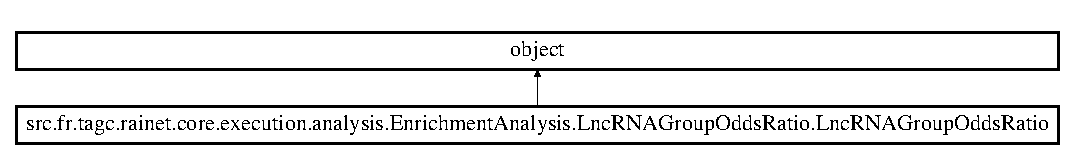
\includegraphics[height=1.707317cm]{classsrc_1_1fr_1_1tagc_1_1rainet_1_1core_1_1execution_1_1analysis_1_1EnrichmentAnalysis_1_1LncRN93e4a312e019c4b142d886126e1373f6}
\end{center}
\end{figure}
\subsection*{Public Member Functions}
\begin{DoxyCompactItemize}
\item 
\hypertarget{classsrc_1_1fr_1_1tagc_1_1rainet_1_1core_1_1execution_1_1analysis_1_1EnrichmentAnalysis_1_1LncRN93e4a312e019c4b142d886126e1373f6_ae9b56f4f382c355a22f41e7390bc09f2}{def {\bfseries \-\_\-\-\_\-init\-\_\-\-\_\-}}\label{classsrc_1_1fr_1_1tagc_1_1rainet_1_1core_1_1execution_1_1analysis_1_1EnrichmentAnalysis_1_1LncRN93e4a312e019c4b142d886126e1373f6_ae9b56f4f382c355a22f41e7390bc09f2}

\item 
\hypertarget{classsrc_1_1fr_1_1tagc_1_1rainet_1_1core_1_1execution_1_1analysis_1_1EnrichmentAnalysis_1_1LncRN93e4a312e019c4b142d886126e1373f6_a30b7d4626408d524334b1454e9e1fa2f}{def {\bfseries read\-\_\-rainet\-\_\-db}}\label{classsrc_1_1fr_1_1tagc_1_1rainet_1_1core_1_1execution_1_1analysis_1_1EnrichmentAnalysis_1_1LncRN93e4a312e019c4b142d886126e1373f6_a30b7d4626408d524334b1454e9e1fa2f}

\item 
\hypertarget{classsrc_1_1fr_1_1tagc_1_1rainet_1_1core_1_1execution_1_1analysis_1_1EnrichmentAnalysis_1_1LncRN93e4a312e019c4b142d886126e1373f6_a7b9e1a0b8dcada36d3cbc463d56fc7fe}{def {\bfseries read\-\_\-annotation\-\_\-file}}\label{classsrc_1_1fr_1_1tagc_1_1rainet_1_1core_1_1execution_1_1analysis_1_1EnrichmentAnalysis_1_1LncRN93e4a312e019c4b142d886126e1373f6_a7b9e1a0b8dcada36d3cbc463d56fc7fe}

\item 
\hypertarget{classsrc_1_1fr_1_1tagc_1_1rainet_1_1core_1_1execution_1_1analysis_1_1EnrichmentAnalysis_1_1LncRN93e4a312e019c4b142d886126e1373f6_a8388019ee172d879203a9a7e7ed18ecb}{def {\bfseries read\-\_\-external\-\_\-files}}\label{classsrc_1_1fr_1_1tagc_1_1rainet_1_1core_1_1execution_1_1analysis_1_1EnrichmentAnalysis_1_1LncRN93e4a312e019c4b142d886126e1373f6_a8388019ee172d879203a9a7e7ed18ecb}

\item 
\hypertarget{classsrc_1_1fr_1_1tagc_1_1rainet_1_1core_1_1execution_1_1analysis_1_1EnrichmentAnalysis_1_1LncRN93e4a312e019c4b142d886126e1373f6_ac88b8504b3229b834ab33c655992a0a7}{def {\bfseries read\-\_\-background\-\_\-list}}\label{classsrc_1_1fr_1_1tagc_1_1rainet_1_1core_1_1execution_1_1analysis_1_1EnrichmentAnalysis_1_1LncRN93e4a312e019c4b142d886126e1373f6_ac88b8504b3229b834ab33c655992a0a7}

\item 
\hypertarget{classsrc_1_1fr_1_1tagc_1_1rainet_1_1core_1_1execution_1_1analysis_1_1EnrichmentAnalysis_1_1LncRN93e4a312e019c4b142d886126e1373f6_a7bee91348a4237ff4dc22dfd182ad9e3}{def {\bfseries calculate\-\_\-odds\-\_\-ratio}}\label{classsrc_1_1fr_1_1tagc_1_1rainet_1_1core_1_1execution_1_1analysis_1_1EnrichmentAnalysis_1_1LncRN93e4a312e019c4b142d886126e1373f6_a7bee91348a4237ff4dc22dfd182ad9e3}

\item 
\hypertarget{classsrc_1_1fr_1_1tagc_1_1rainet_1_1core_1_1execution_1_1analysis_1_1EnrichmentAnalysis_1_1LncRN93e4a312e019c4b142d886126e1373f6_a84b4fa7ee1a8268702f24d8b0f9cca3d}{def {\bfseries run}}\label{classsrc_1_1fr_1_1tagc_1_1rainet_1_1core_1_1execution_1_1analysis_1_1EnrichmentAnalysis_1_1LncRN93e4a312e019c4b142d886126e1373f6_a84b4fa7ee1a8268702f24d8b0f9cca3d}

\end{DoxyCompactItemize}
\subsection*{Static Public Member Functions}
\begin{DoxyCompactItemize}
\item 
\hypertarget{classsrc_1_1fr_1_1tagc_1_1rainet_1_1core_1_1execution_1_1analysis_1_1EnrichmentAnalysis_1_1LncRN93e4a312e019c4b142d886126e1373f6_a196a1a693c49c4b8eff3a731e5395979}{def {\bfseries fisher\-\_\-exact\-\_\-test}}\label{classsrc_1_1fr_1_1tagc_1_1rainet_1_1core_1_1execution_1_1analysis_1_1EnrichmentAnalysis_1_1LncRN93e4a312e019c4b142d886126e1373f6_a196a1a693c49c4b8eff3a731e5395979}

\end{DoxyCompactItemize}
\subsection*{Public Attributes}
\begin{DoxyCompactItemize}
\item 
\hypertarget{classsrc_1_1fr_1_1tagc_1_1rainet_1_1core_1_1execution_1_1analysis_1_1EnrichmentAnalysis_1_1LncRN93e4a312e019c4b142d886126e1373f6_ad0087462fd17d275bdf105381886ec92}{{\bfseries annotation\-File}}\label{classsrc_1_1fr_1_1tagc_1_1rainet_1_1core_1_1execution_1_1analysis_1_1EnrichmentAnalysis_1_1LncRN93e4a312e019c4b142d886126e1373f6_ad0087462fd17d275bdf105381886ec92}

\item 
\hypertarget{classsrc_1_1fr_1_1tagc_1_1rainet_1_1core_1_1execution_1_1analysis_1_1EnrichmentAnalysis_1_1LncRN93e4a312e019c4b142d886126e1373f6_a2eaadb8ee526d554e8b8708566fa1fa7}{{\bfseries external\-Files}}\label{classsrc_1_1fr_1_1tagc_1_1rainet_1_1core_1_1execution_1_1analysis_1_1EnrichmentAnalysis_1_1LncRN93e4a312e019c4b142d886126e1373f6_a2eaadb8ee526d554e8b8708566fa1fa7}

\item 
\hypertarget{classsrc_1_1fr_1_1tagc_1_1rainet_1_1core_1_1execution_1_1analysis_1_1EnrichmentAnalysis_1_1LncRN93e4a312e019c4b142d886126e1373f6_aadca07e864cc85ea05afe17aae2d251f}{{\bfseries background\-List}}\label{classsrc_1_1fr_1_1tagc_1_1rainet_1_1core_1_1execution_1_1analysis_1_1EnrichmentAnalysis_1_1LncRN93e4a312e019c4b142d886126e1373f6_aadca07e864cc85ea05afe17aae2d251f}

\item 
\hypertarget{classsrc_1_1fr_1_1tagc_1_1rainet_1_1core_1_1execution_1_1analysis_1_1EnrichmentAnalysis_1_1LncRN93e4a312e019c4b142d886126e1373f6_a830460d7f9fd1c4fc29897b51a554842}{{\bfseries output\-File}}\label{classsrc_1_1fr_1_1tagc_1_1rainet_1_1core_1_1execution_1_1analysis_1_1EnrichmentAnalysis_1_1LncRN93e4a312e019c4b142d886126e1373f6_a830460d7f9fd1c4fc29897b51a554842}

\item 
\hypertarget{classsrc_1_1fr_1_1tagc_1_1rainet_1_1core_1_1execution_1_1analysis_1_1EnrichmentAnalysis_1_1LncRN93e4a312e019c4b142d886126e1373f6_a9a62a546166ed7ef6773b880c3eb28e5}{{\bfseries use\-Genes}}\label{classsrc_1_1fr_1_1tagc_1_1rainet_1_1core_1_1execution_1_1analysis_1_1EnrichmentAnalysis_1_1LncRN93e4a312e019c4b142d886126e1373f6_a9a62a546166ed7ef6773b880c3eb28e5}

\item 
\hypertarget{classsrc_1_1fr_1_1tagc_1_1rainet_1_1core_1_1execution_1_1analysis_1_1EnrichmentAnalysis_1_1LncRN93e4a312e019c4b142d886126e1373f6_a7c5269170ef0d588b6ff320a7b827579}{{\bfseries rainet\-D\-B}}\label{classsrc_1_1fr_1_1tagc_1_1rainet_1_1core_1_1execution_1_1analysis_1_1EnrichmentAnalysis_1_1LncRN93e4a312e019c4b142d886126e1373f6_a7c5269170ef0d588b6ff320a7b827579}

\item 
\hypertarget{classsrc_1_1fr_1_1tagc_1_1rainet_1_1core_1_1execution_1_1analysis_1_1EnrichmentAnalysis_1_1LncRN93e4a312e019c4b142d886126e1373f6_a0b5b8db1b4df6bf935261bc56441cd4c}{{\bfseries sql\-\_\-session}}\label{classsrc_1_1fr_1_1tagc_1_1rainet_1_1core_1_1execution_1_1analysis_1_1EnrichmentAnalysis_1_1LncRN93e4a312e019c4b142d886126e1373f6_a0b5b8db1b4df6bf935261bc56441cd4c}

\item 
\hypertarget{classsrc_1_1fr_1_1tagc_1_1rainet_1_1core_1_1execution_1_1analysis_1_1EnrichmentAnalysis_1_1LncRN93e4a312e019c4b142d886126e1373f6_ac0f510b690ae48627243f73b21ad40e3}{{\bfseries rna\-Cross\-Reference}}\label{classsrc_1_1fr_1_1tagc_1_1rainet_1_1core_1_1execution_1_1analysis_1_1EnrichmentAnalysis_1_1LncRN93e4a312e019c4b142d886126e1373f6_ac0f510b690ae48627243f73b21ad40e3}

\item 
\hypertarget{classsrc_1_1fr_1_1tagc_1_1rainet_1_1core_1_1execution_1_1analysis_1_1EnrichmentAnalysis_1_1LncRN93e4a312e019c4b142d886126e1373f6_acd23227834ba80e895df9ca2f2bf0f5f}{{\bfseries transcript\-Annotation}}\label{classsrc_1_1fr_1_1tagc_1_1rainet_1_1core_1_1execution_1_1analysis_1_1EnrichmentAnalysis_1_1LncRN93e4a312e019c4b142d886126e1373f6_acd23227834ba80e895df9ca2f2bf0f5f}

\item 
\hypertarget{classsrc_1_1fr_1_1tagc_1_1rainet_1_1core_1_1execution_1_1analysis_1_1EnrichmentAnalysis_1_1LncRN93e4a312e019c4b142d886126e1373f6_ae976ccbe76091b6c45e9f09fba9c0689}{{\bfseries group\-Transcripts}}\label{classsrc_1_1fr_1_1tagc_1_1rainet_1_1core_1_1execution_1_1analysis_1_1EnrichmentAnalysis_1_1LncRN93e4a312e019c4b142d886126e1373f6_ae976ccbe76091b6c45e9f09fba9c0689}

\item 
\hypertarget{classsrc_1_1fr_1_1tagc_1_1rainet_1_1core_1_1execution_1_1analysis_1_1EnrichmentAnalysis_1_1LncRN93e4a312e019c4b142d886126e1373f6_abc6d566edf10ac9ac5fb4335a506d25e}{{\bfseries external\-Lists}}\label{classsrc_1_1fr_1_1tagc_1_1rainet_1_1core_1_1execution_1_1analysis_1_1EnrichmentAnalysis_1_1LncRN93e4a312e019c4b142d886126e1373f6_abc6d566edf10ac9ac5fb4335a506d25e}

\item 
\hyperlink{classsrc_1_1fr_1_1tagc_1_1rainet_1_1core_1_1execution_1_1analysis_1_1EnrichmentAnalysis_1_1LncRN93e4a312e019c4b142d886126e1373f6_a2e1af37469e9a8f2edd6287852d15571}{background\-Transcripts}
\begin{DoxyCompactList}\small\item\em annotation transcripts \end{DoxyCompactList}\item 
\hypertarget{classsrc_1_1fr_1_1tagc_1_1rainet_1_1core_1_1execution_1_1analysis_1_1EnrichmentAnalysis_1_1LncRN93e4a312e019c4b142d886126e1373f6_ab80c70500941c8d147ffe1729e9fcb82}{{\bfseries filtered\-External\-Lists}}\label{classsrc_1_1fr_1_1tagc_1_1rainet_1_1core_1_1execution_1_1analysis_1_1EnrichmentAnalysis_1_1LncRN93e4a312e019c4b142d886126e1373f6_ab80c70500941c8d147ffe1729e9fcb82}

\item 
\hypertarget{classsrc_1_1fr_1_1tagc_1_1rainet_1_1core_1_1execution_1_1analysis_1_1EnrichmentAnalysis_1_1LncRN93e4a312e019c4b142d886126e1373f6_a2ab8cf438c402f7febff345eeb201937}{{\bfseries filtered\-Annotation\-Transcripts}}\label{classsrc_1_1fr_1_1tagc_1_1rainet_1_1core_1_1execution_1_1analysis_1_1EnrichmentAnalysis_1_1LncRN93e4a312e019c4b142d886126e1373f6_a2ab8cf438c402f7febff345eeb201937}

\item 
\hypertarget{classsrc_1_1fr_1_1tagc_1_1rainet_1_1core_1_1execution_1_1analysis_1_1EnrichmentAnalysis_1_1LncRN93e4a312e019c4b142d886126e1373f6_a7d7880760f7ad008daf616d3c7e14130}{{\bfseries data\-Store}}\label{classsrc_1_1fr_1_1tagc_1_1rainet_1_1core_1_1execution_1_1analysis_1_1EnrichmentAnalysis_1_1LncRN93e4a312e019c4b142d886126e1373f6_a7d7880760f7ad008daf616d3c7e14130}

\end{DoxyCompactItemize}
\subsection*{Static Public Attributes}
\begin{DoxyCompactItemize}
\item 
\hypertarget{classsrc_1_1fr_1_1tagc_1_1rainet_1_1core_1_1execution_1_1analysis_1_1EnrichmentAnalysis_1_1LncRN93e4a312e019c4b142d886126e1373f6_a6cd496a9f9e41de6016d46cf009f4764}{string {\bfseries A\-R\-G\-U\-M\-E\-N\-T\-\_\-\-R\-A\-I\-N\-E\-T\-\_\-\-D\-B\-\_\-\-D\-E\-F\-A\-U\-L\-T} = \char`\"{}\char`\"{}}\label{classsrc_1_1fr_1_1tagc_1_1rainet_1_1core_1_1execution_1_1analysis_1_1EnrichmentAnalysis_1_1LncRN93e4a312e019c4b142d886126e1373f6_a6cd496a9f9e41de6016d46cf009f4764}

\item 
\hypertarget{classsrc_1_1fr_1_1tagc_1_1rainet_1_1core_1_1execution_1_1analysis_1_1EnrichmentAnalysis_1_1LncRN93e4a312e019c4b142d886126e1373f6_a188ab546b7c1b61c2980acd6c221cefd}{int {\bfseries A\-N\-N\-O\-T\-A\-T\-I\-O\-N\-\_\-\-F\-I\-L\-E\-\_\-\-I\-D\-\_\-\-C\-O\-L\-U\-M\-N} = 0}\label{classsrc_1_1fr_1_1tagc_1_1rainet_1_1core_1_1execution_1_1analysis_1_1EnrichmentAnalysis_1_1LncRN93e4a312e019c4b142d886126e1373f6_a188ab546b7c1b61c2980acd6c221cefd}

\item 
\hypertarget{classsrc_1_1fr_1_1tagc_1_1rainet_1_1core_1_1execution_1_1analysis_1_1EnrichmentAnalysis_1_1LncRN93e4a312e019c4b142d886126e1373f6_a73470ee201046db4b0041f6ecfde0a15}{int {\bfseries A\-N\-N\-O\-T\-A\-T\-I\-O\-N\-\_\-\-F\-I\-L\-E\-\_\-\-A\-N\-N\-O\-T\-A\-T\-I\-O\-N\-\_\-\-C\-O\-L\-U\-M\-N} = 1}\label{classsrc_1_1fr_1_1tagc_1_1rainet_1_1core_1_1execution_1_1analysis_1_1EnrichmentAnalysis_1_1LncRN93e4a312e019c4b142d886126e1373f6_a73470ee201046db4b0041f6ecfde0a15}

\end{DoxyCompactItemize}


\subsection{Member Data Documentation}
\hypertarget{classsrc_1_1fr_1_1tagc_1_1rainet_1_1core_1_1execution_1_1analysis_1_1EnrichmentAnalysis_1_1LncRN93e4a312e019c4b142d886126e1373f6_a2e1af37469e9a8f2edd6287852d15571}{\index{src\-::fr\-::tagc\-::rainet\-::core\-::execution\-::analysis\-::\-Enrichment\-Analysis\-::\-Lnc\-R\-N\-A\-Group\-Odds\-Ratio\-::\-Lnc\-R\-N\-A\-Group\-Odds\-Ratio@{src\-::fr\-::tagc\-::rainet\-::core\-::execution\-::analysis\-::\-Enrichment\-Analysis\-::\-Lnc\-R\-N\-A\-Group\-Odds\-Ratio\-::\-Lnc\-R\-N\-A\-Group\-Odds\-Ratio}!background\-Transcripts@{background\-Transcripts}}
\index{background\-Transcripts@{background\-Transcripts}!src::fr::tagc::rainet::core::execution::analysis::EnrichmentAnalysis::LncRNAGroupOddsRatio::LncRNAGroupOddsRatio@{src\-::fr\-::tagc\-::rainet\-::core\-::execution\-::analysis\-::\-Enrichment\-Analysis\-::\-Lnc\-R\-N\-A\-Group\-Odds\-Ratio\-::\-Lnc\-R\-N\-A\-Group\-Odds\-Ratio}}
\subsubsection[{background\-Transcripts}]{\setlength{\rightskip}{0pt plus 5cm}src.\-fr.\-tagc.\-rainet.\-core.\-execution.\-analysis.\-Enrichment\-Analysis.\-Lnc\-R\-N\-A\-Group\-Odds\-Ratio.\-Lnc\-R\-N\-A\-Group\-Odds\-Ratio.\-background\-Transcripts}}\label{classsrc_1_1fr_1_1tagc_1_1rainet_1_1core_1_1execution_1_1analysis_1_1EnrichmentAnalysis_1_1LncRN93e4a312e019c4b142d886126e1373f6_a2e1af37469e9a8f2edd6287852d15571}


annotation transcripts 

External transcript lists 

The documentation for this class was generated from the following file\-:\begin{DoxyCompactItemize}
\item 
src/fr/tagc/rainet/core/execution/analysis/\-Enrichment\-Analysis/Lnc\-R\-N\-A\-Group\-Odds\-Ratio.\-py\end{DoxyCompactItemize}

\hypertarget{classLncRNAGroupOddsRatioUnittest_1_1LncRNAGroupOddsRatioUnittest}{\section{Lnc\-R\-N\-A\-Group\-Odds\-Ratio\-Unittest.\-Lnc\-R\-N\-A\-Group\-Odds\-Ratio\-Unittest Class Reference}
\label{classLncRNAGroupOddsRatioUnittest_1_1LncRNAGroupOddsRatioUnittest}\index{Lnc\-R\-N\-A\-Group\-Odds\-Ratio\-Unittest.\-Lnc\-R\-N\-A\-Group\-Odds\-Ratio\-Unittest@{Lnc\-R\-N\-A\-Group\-Odds\-Ratio\-Unittest.\-Lnc\-R\-N\-A\-Group\-Odds\-Ratio\-Unittest}}
}
Inheritance diagram for Lnc\-R\-N\-A\-Group\-Odds\-Ratio\-Unittest.\-Lnc\-R\-N\-A\-Group\-Odds\-Ratio\-Unittest\-:\begin{figure}[H]
\begin{center}
\leavevmode
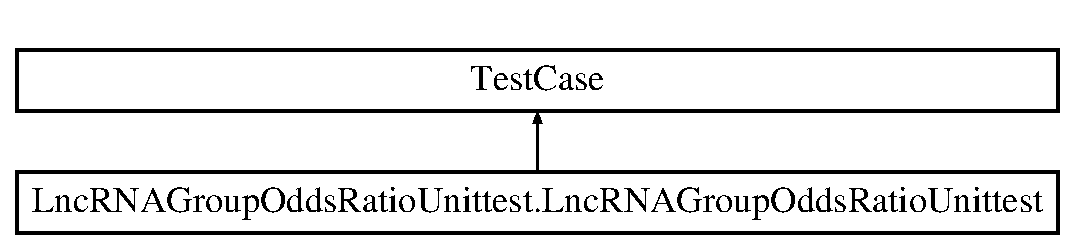
\includegraphics[height=2.000000cm]{classLncRNAGroupOddsRatioUnittest_1_1LncRNAGroupOddsRatioUnittest}
\end{center}
\end{figure}
\subsection*{Public Member Functions}
\begin{DoxyCompactItemize}
\item 
\hypertarget{classLncRNAGroupOddsRatioUnittest_1_1LncRNAGroupOddsRatioUnittest_a14e3e7534ec9e1dad1526a54ad95f1b8}{def {\bfseries set\-Up}}\label{classLncRNAGroupOddsRatioUnittest_1_1LncRNAGroupOddsRatioUnittest_a14e3e7534ec9e1dad1526a54ad95f1b8}

\item 
\hypertarget{classLncRNAGroupOddsRatioUnittest_1_1LncRNAGroupOddsRatioUnittest_a16110ec0f31079f6f2d9175d62d686ca}{def {\bfseries test\-\_\-read\-\_\-rainet\-\_\-db}}\label{classLncRNAGroupOddsRatioUnittest_1_1LncRNAGroupOddsRatioUnittest_a16110ec0f31079f6f2d9175d62d686ca}

\item 
\hypertarget{classLncRNAGroupOddsRatioUnittest_1_1LncRNAGroupOddsRatioUnittest_a8300c0f2055246ea45673eae6af7a07c}{def {\bfseries test\-\_\-read\-\_\-annotation\-\_\-file}}\label{classLncRNAGroupOddsRatioUnittest_1_1LncRNAGroupOddsRatioUnittest_a8300c0f2055246ea45673eae6af7a07c}

\item 
\hypertarget{classLncRNAGroupOddsRatioUnittest_1_1LncRNAGroupOddsRatioUnittest_a3580befe4eb1b341be4cebfed5fffb26}{def {\bfseries test\-\_\-read\-\_\-annotation\-\_\-file\-\_\-transcript\-\_\-id}}\label{classLncRNAGroupOddsRatioUnittest_1_1LncRNAGroupOddsRatioUnittest_a3580befe4eb1b341be4cebfed5fffb26}

\item 
\hypertarget{classLncRNAGroupOddsRatioUnittest_1_1LncRNAGroupOddsRatioUnittest_ac539311cc6d96d3eba690bdac96f0e06}{def {\bfseries test\-\_\-read\-\_\-external\-\_\-files}}\label{classLncRNAGroupOddsRatioUnittest_1_1LncRNAGroupOddsRatioUnittest_ac539311cc6d96d3eba690bdac96f0e06}

\item 
\hypertarget{classLncRNAGroupOddsRatioUnittest_1_1LncRNAGroupOddsRatioUnittest_a44db6f884806e4c185f38d7232de0ab7}{def {\bfseries test\-\_\-read\-\_\-background\-\_\-list}}\label{classLncRNAGroupOddsRatioUnittest_1_1LncRNAGroupOddsRatioUnittest_a44db6f884806e4c185f38d7232de0ab7}

\item 
\hypertarget{classLncRNAGroupOddsRatioUnittest_1_1LncRNAGroupOddsRatioUnittest_a8df3c3545bba4b9d426675307168dd47}{def {\bfseries test\-\_\-calculate\-\_\-odds\-\_\-ratio}}\label{classLncRNAGroupOddsRatioUnittest_1_1LncRNAGroupOddsRatioUnittest_a8df3c3545bba4b9d426675307168dd47}

\item 
\hypertarget{classLncRNAGroupOddsRatioUnittest_1_1LncRNAGroupOddsRatioUnittest_ae504e72cfe477f78d1295ead92acdd2c}{def {\bfseries test\-\_\-fisher\-\_\-exact\-\_\-test}}\label{classLncRNAGroupOddsRatioUnittest_1_1LncRNAGroupOddsRatioUnittest_ae504e72cfe477f78d1295ead92acdd2c}

\end{DoxyCompactItemize}
\subsection*{Public Attributes}
\begin{DoxyCompactItemize}
\item 
\hypertarget{classLncRNAGroupOddsRatioUnittest_1_1LncRNAGroupOddsRatioUnittest_a4d4062f5ebe19a27a13b6677911b7f2e}{{\bfseries annotation\-File}}\label{classLncRNAGroupOddsRatioUnittest_1_1LncRNAGroupOddsRatioUnittest_a4d4062f5ebe19a27a13b6677911b7f2e}

\item 
\hypertarget{classLncRNAGroupOddsRatioUnittest_1_1LncRNAGroupOddsRatioUnittest_ad508e3350bcac8fc78c281978468948a}{{\bfseries external\-Files}}\label{classLncRNAGroupOddsRatioUnittest_1_1LncRNAGroupOddsRatioUnittest_ad508e3350bcac8fc78c281978468948a}

\item 
\hypertarget{classLncRNAGroupOddsRatioUnittest_1_1LncRNAGroupOddsRatioUnittest_a40eef52a7113871a5339b94d65d1ae7f}{{\bfseries background\-List}}\label{classLncRNAGroupOddsRatioUnittest_1_1LncRNAGroupOddsRatioUnittest_a40eef52a7113871a5339b94d65d1ae7f}

\item 
\hypertarget{classLncRNAGroupOddsRatioUnittest_1_1LncRNAGroupOddsRatioUnittest_afe06014218a8078d31d70f870e4faefb}{{\bfseries output\-Folder}}\label{classLncRNAGroupOddsRatioUnittest_1_1LncRNAGroupOddsRatioUnittest_afe06014218a8078d31d70f870e4faefb}

\item 
\hypertarget{classLncRNAGroupOddsRatioUnittest_1_1LncRNAGroupOddsRatioUnittest_a255025df34632596174c0776273e0a02}{{\bfseries use\-Genes}}\label{classLncRNAGroupOddsRatioUnittest_1_1LncRNAGroupOddsRatioUnittest_a255025df34632596174c0776273e0a02}

\item 
\hypertarget{classLncRNAGroupOddsRatioUnittest_1_1LncRNAGroupOddsRatioUnittest_a26a647f97985e4c20009e838cbad0a96}{{\bfseries rainet\-D\-B}}\label{classLncRNAGroupOddsRatioUnittest_1_1LncRNAGroupOddsRatioUnittest_a26a647f97985e4c20009e838cbad0a96}

\item 
\hypertarget{classLncRNAGroupOddsRatioUnittest_1_1LncRNAGroupOddsRatioUnittest_a24b2ff6eb8055b4aff81f0067681e74c}{{\bfseries run}}\label{classLncRNAGroupOddsRatioUnittest_1_1LncRNAGroupOddsRatioUnittest_a24b2ff6eb8055b4aff81f0067681e74c}

\end{DoxyCompactItemize}


The documentation for this class was generated from the following file\-:\begin{DoxyCompactItemize}
\item 
test/fr/tagc/rainet/core/execution/analysis/\-Enrichment\-Analysis/Lnc\-R\-N\-A\-Group\-Odds\-Ratio\-Unittest.\-py\end{DoxyCompactItemize}

\hypertarget{classLncRNAScore_1_1LncRNAScore}{\section{Lnc\-R\-N\-A\-Score.\-Lnc\-R\-N\-A\-Score Class Reference}
\label{classLncRNAScore_1_1LncRNAScore}\index{Lnc\-R\-N\-A\-Score.\-Lnc\-R\-N\-A\-Score@{Lnc\-R\-N\-A\-Score.\-Lnc\-R\-N\-A\-Score}}
}
Inheritance diagram for Lnc\-R\-N\-A\-Score.\-Lnc\-R\-N\-A\-Score\-:\begin{figure}[H]
\begin{center}
\leavevmode
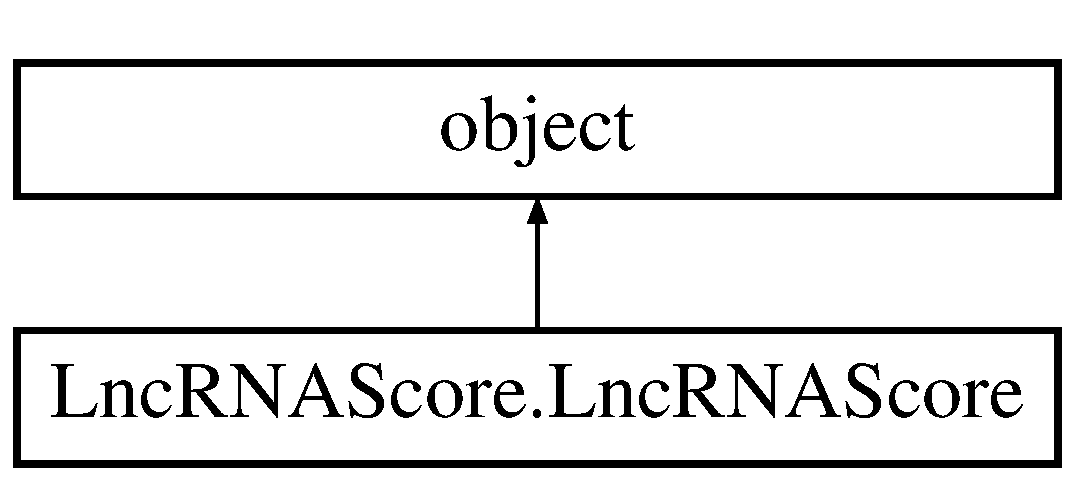
\includegraphics[height=2.000000cm]{classLncRNAScore_1_1LncRNAScore}
\end{center}
\end{figure}
\subsection*{Public Member Functions}
\begin{DoxyCompactItemize}
\item 
\hypertarget{classLncRNAScore_1_1LncRNAScore_a18cc7ab3e946f047a3646d8e23f1c61e}{def {\bfseries \-\_\-\-\_\-init\-\_\-\-\_\-}}\label{classLncRNAScore_1_1LncRNAScore_a18cc7ab3e946f047a3646d8e23f1c61e}

\item 
\hypertarget{classLncRNAScore_1_1LncRNAScore_aae9bee080459aee4bbd149f52612b4bb}{def {\bfseries rna\-\_\-cross\-\_\-references}}\label{classLncRNAScore_1_1LncRNAScore_aae9bee080459aee4bbd149f52612b4bb}

\item 
\hypertarget{classLncRNAScore_1_1LncRNAScore_a244e3672ae4c7333a27508086158ac82}{def {\bfseries read\-\_\-annotation\-\_\-file}}\label{classLncRNAScore_1_1LncRNAScore_a244e3672ae4c7333a27508086158ac82}

\item 
\hypertarget{classLncRNAScore_1_1LncRNAScore_a99bebe98d4bf1ac2b23ff0edcaaaf7e4}{def {\bfseries read\-\_\-interaction\-\_\-file}}\label{classLncRNAScore_1_1LncRNAScore_a99bebe98d4bf1ac2b23ff0edcaaaf7e4}

\end{DoxyCompactItemize}
\subsection*{Public Attributes}
\begin{DoxyCompactItemize}
\item 
\hypertarget{classLncRNAScore_1_1LncRNAScore_a2e04bc66f1a509b8f3310ff48e0f1dfb}{{\bfseries annotation\-File}}\label{classLncRNAScore_1_1LncRNAScore_a2e04bc66f1a509b8f3310ff48e0f1dfb}

\item 
\hypertarget{classLncRNAScore_1_1LncRNAScore_a5dc0b2a4e8479ad7ff5beefbb0afe7b6}{{\bfseries interaction\-File}}\label{classLncRNAScore_1_1LncRNAScore_a5dc0b2a4e8479ad7ff5beefbb0afe7b6}

\item 
\hypertarget{classLncRNAScore_1_1LncRNAScore_a36d347551fe48ad374f9192e1d7728f9}{{\bfseries rainet\-D\-B}}\label{classLncRNAScore_1_1LncRNAScore_a36d347551fe48ad374f9192e1d7728f9}

\item 
\hypertarget{classLncRNAScore_1_1LncRNAScore_af5b1c272c2a4a55e6ddb008ecd4c50eb}{{\bfseries output\-Folder}}\label{classLncRNAScore_1_1LncRNAScore_af5b1c272c2a4a55e6ddb008ecd4c50eb}

\item 
\hypertarget{classLncRNAScore_1_1LncRNAScore_ae8b4e05a046641abe060d76e8e9a6826}{{\bfseries mask\-Multiple}}\label{classLncRNAScore_1_1LncRNAScore_ae8b4e05a046641abe060d76e8e9a6826}

\item 
\hypertarget{classLncRNAScore_1_1LncRNAScore_a2a33d881b5b855a744c1797185b100f7}{{\bfseries annotation\-Column}}\label{classLncRNAScore_1_1LncRNAScore_a2a33d881b5b855a744c1797185b100f7}

\item 
\hypertarget{classLncRNAScore_1_1LncRNAScore_a678a5c34d0b3bba3d335794e2184b3c1}{{\bfseries id\-Column}}\label{classLncRNAScore_1_1LncRNAScore_a678a5c34d0b3bba3d335794e2184b3c1}

\item 
\hypertarget{classLncRNAScore_1_1LncRNAScore_a09d6f19803dfb51fa7a63aa9db53a48b}{{\bfseries no\-Annotation\-Tag}}\label{classLncRNAScore_1_1LncRNAScore_a09d6f19803dfb51fa7a63aa9db53a48b}

\item 
\hypertarget{classLncRNAScore_1_1LncRNAScore_a7d954a064a1b3df96cf50b9e66206eba}{{\bfseries cross\-Reference}}\label{classLncRNAScore_1_1LncRNAScore_a7d954a064a1b3df96cf50b9e66206eba}

\item 
\hypertarget{classLncRNAScore_1_1LncRNAScore_a393fd5d272848838a5bfc74c6f6a294d}{{\bfseries sql\-\_\-session}}\label{classLncRNAScore_1_1LncRNAScore_a393fd5d272848838a5bfc74c6f6a294d}

\item 
\hypertarget{classLncRNAScore_1_1LncRNAScore_ad0993c829e21d97af9a2eaca3101b1ac}{{\bfseries rna\-Gene\-Reference}}\label{classLncRNAScore_1_1LncRNAScore_ad0993c829e21d97af9a2eaca3101b1ac}

\end{DoxyCompactItemize}
\subsection*{Static Public Attributes}
\begin{DoxyCompactItemize}
\item 
\hypertarget{classLncRNAScore_1_1LncRNAScore_aa7bc87b3f5b74d5808bbecb9eb0c4788}{string {\bfseries I\-D\-\_\-\-M\-A\-P\-P\-I\-N\-G\-\_\-\-O\-U\-T\-P\-U\-T\-\_\-\-F\-I\-L\-E} = \char`\"{}/transcripts\-\_\-ensembl\-\_\-id.\-tsv\char`\"{}}\label{classLncRNAScore_1_1LncRNAScore_aa7bc87b3f5b74d5808bbecb9eb0c4788}

\item 
\hypertarget{classLncRNAScore_1_1LncRNAScore_abfe8e46ab578a5172c4f675a9240dd32}{string {\bfseries A\-N\-N\-O\-T\-A\-T\-I\-O\-N\-\_\-\-O\-U\-T\-P\-U\-T\-\_\-\-F\-I\-L\-E} = \char`\"{}/annotated\-\_\-interactions.\-tsv\char`\"{}}\label{classLncRNAScore_1_1LncRNAScore_abfe8e46ab578a5172c4f675a9240dd32}

\item 
\hypertarget{classLncRNAScore_1_1LncRNAScore_a76bd5d7ff4b1c1bb59fb1f79f547982f}{string {\bfseries S\-E\-V\-E\-R\-A\-L\-\_\-\-A\-N\-N\-O\-T\-A\-T\-I\-O\-N\-\_\-\-T\-A\-G} = \char`\"{}Overlapping\-\_\-annotations\char`\"{}}\label{classLncRNAScore_1_1LncRNAScore_a76bd5d7ff4b1c1bb59fb1f79f547982f}

\end{DoxyCompactItemize}


The documentation for this class was generated from the following file\-:\begin{DoxyCompactItemize}
\item 
src/fr/tagc/rainet/core/execution/analysis/lnc\-R\-N\-A\-\_\-analysis/Lnc\-R\-N\-A\-Score.\-py\end{DoxyCompactItemize}

\hypertarget{classsrc_1_1core_1_1util_1_1log_1_1Logger_1_1Logger}{\section{src.\-core.\-util.\-log.\-Logger.\-Logger Class Reference}
\label{classsrc_1_1core_1_1util_1_1log_1_1Logger_1_1Logger}\index{src.\-core.\-util.\-log.\-Logger.\-Logger@{src.\-core.\-util.\-log.\-Logger.\-Logger}}
}


This class is a singleton used to manage logging It contains several method to add log at different level and manage both output to file and standard output.  


Inheritance diagram for src.\-core.\-util.\-log.\-Logger.\-Logger\-:\begin{figure}[H]
\begin{center}
\leavevmode
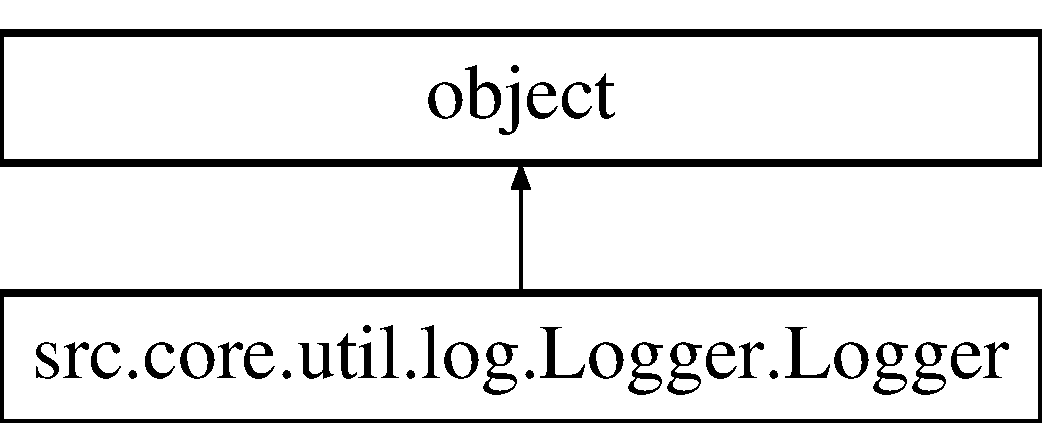
\includegraphics[height=2.000000cm]{classsrc_1_1core_1_1util_1_1log_1_1Logger_1_1Logger}
\end{center}
\end{figure}
\subsection*{Public Member Functions}
\begin{DoxyCompactItemize}
\item 
\hypertarget{classsrc_1_1core_1_1util_1_1log_1_1Logger_1_1Logger_a6bef702bcc63f86a2f56cc71c23f879e}{def {\bfseries \-\_\-\-\_\-init\-\_\-\-\_\-}}\label{classsrc_1_1core_1_1util_1_1log_1_1Logger_1_1Logger_a6bef702bcc63f86a2f56cc71c23f879e}

\item 
\hypertarget{classsrc_1_1core_1_1util_1_1log_1_1Logger_1_1Logger_a63dae9b40528be2bfeac4ddf03242616}{def {\bfseries set\-Logger}}\label{classsrc_1_1core_1_1util_1_1log_1_1Logger_1_1Logger_a63dae9b40528be2bfeac4ddf03242616}

\item 
def \hyperlink{classsrc_1_1core_1_1util_1_1log_1_1Logger_1_1Logger_ac90ece7c1404d072a0a9b78a2b7cec2c}{set\-\_\-level}
\begin{DoxyCompactList}\small\item\em Set the level of verbosity to the given level. \end{DoxyCompactList}\item 
\hypertarget{classsrc_1_1core_1_1util_1_1log_1_1Logger_1_1Logger_ab5484593e2fa5987516e8fa52d237e29}{def {\bfseries debug}}\label{classsrc_1_1core_1_1util_1_1log_1_1Logger_1_1Logger_ab5484593e2fa5987516e8fa52d237e29}

\item 
\hypertarget{classsrc_1_1core_1_1util_1_1log_1_1Logger_1_1Logger_a516504b83a8435772584ece6eafb152c}{def {\bfseries info}}\label{classsrc_1_1core_1_1util_1_1log_1_1Logger_1_1Logger_a516504b83a8435772584ece6eafb152c}

\item 
\hypertarget{classsrc_1_1core_1_1util_1_1log_1_1Logger_1_1Logger_a33638f7efac3983c4500574d46c40383}{def {\bfseries warning}}\label{classsrc_1_1core_1_1util_1_1log_1_1Logger_1_1Logger_a33638f7efac3983c4500574d46c40383}

\item 
\hypertarget{classsrc_1_1core_1_1util_1_1log_1_1Logger_1_1Logger_a922968c5070f425422bd089493b507b0}{def {\bfseries error}}\label{classsrc_1_1core_1_1util_1_1log_1_1Logger_1_1Logger_a922968c5070f425422bd089493b507b0}

\item 
\hypertarget{classsrc_1_1core_1_1util_1_1log_1_1Logger_1_1Logger_a7de8ea2746a8beea5dbadd5f0d629f8f}{def {\bfseries critical}}\label{classsrc_1_1core_1_1util_1_1log_1_1Logger_1_1Logger_a7de8ea2746a8beea5dbadd5f0d629f8f}

\end{DoxyCompactItemize}
\subsection*{Static Public Member Functions}
\begin{DoxyCompactItemize}
\item 
\hypertarget{classsrc_1_1core_1_1util_1_1log_1_1Logger_1_1Logger_ada4abcd33038a24673dab983551410e9}{def {\bfseries get\-\_\-instance}}\label{classsrc_1_1core_1_1util_1_1log_1_1Logger_1_1Logger_ada4abcd33038a24673dab983551410e9}

\end{DoxyCompactItemize}
\subsection*{Public Attributes}
\begin{DoxyCompactItemize}
\item 
\hypertarget{classsrc_1_1core_1_1util_1_1log_1_1Logger_1_1Logger_a9d9e84ff94372c1e5df22ad924cd7538}{{\bfseries logg}}\label{classsrc_1_1core_1_1util_1_1log_1_1Logger_1_1Logger_a9d9e84ff94372c1e5df22ad924cd7538}

\item 
\hypertarget{classsrc_1_1core_1_1util_1_1log_1_1Logger_1_1Logger_a7df0c0e686b7013df71564196209b627}{{\bfseries file\-Handler}}\label{classsrc_1_1core_1_1util_1_1log_1_1Logger_1_1Logger_a7df0c0e686b7013df71564196209b627}

\item 
\hypertarget{classsrc_1_1core_1_1util_1_1log_1_1Logger_1_1Logger_a0ca2b895b72e12f474f13e36fe774a85}{{\bfseries stream\-Handler}}\label{classsrc_1_1core_1_1util_1_1log_1_1Logger_1_1Logger_a0ca2b895b72e12f474f13e36fe774a85}

\end{DoxyCompactItemize}


\subsection{Detailed Description}
This class is a singleton used to manage logging It contains several method to add log at different level and manage both output to file and standard output. 

\subsection{Member Function Documentation}
\hypertarget{classsrc_1_1core_1_1util_1_1log_1_1Logger_1_1Logger_ac90ece7c1404d072a0a9b78a2b7cec2c}{\index{src\-::core\-::util\-::log\-::\-Logger\-::\-Logger@{src\-::core\-::util\-::log\-::\-Logger\-::\-Logger}!set\-\_\-level@{set\-\_\-level}}
\index{set\-\_\-level@{set\-\_\-level}!src::core::util::log::Logger::Logger@{src\-::core\-::util\-::log\-::\-Logger\-::\-Logger}}
\subsubsection[{set\-\_\-level}]{\setlength{\rightskip}{0pt plus 5cm}def src.\-core.\-util.\-log.\-Logger.\-Logger.\-set\-\_\-level (
\begin{DoxyParamCaption}
\item[{}]{self, }
\item[{}]{level}
\end{DoxyParamCaption}
)}}\label{classsrc_1_1core_1_1util_1_1log_1_1Logger_1_1Logger_ac90ece7c1404d072a0a9b78a2b7cec2c}


Set the level of verbosity to the given level. 


\begin{DoxyParams}{Parameters}
{\em level} & \-: string -\/ The level of verbosity \\
\hline
\end{DoxyParams}


The documentation for this class was generated from the following file\-:\begin{DoxyCompactItemize}
\item 
rbp-\/motif/src/core/util/log/Logger.\-py\end{DoxyCompactItemize}

\hypertarget{classsrc_1_1fr_1_1tagc_1_1rainet_1_1core_1_1util_1_1log_1_1Logger_1_1Logger}{\section{src.\-fr.\-tagc.\-rainet.\-core.\-util.\-log.\-Logger.\-Logger Class Reference}
\label{classsrc_1_1fr_1_1tagc_1_1rainet_1_1core_1_1util_1_1log_1_1Logger_1_1Logger}\index{src.\-fr.\-tagc.\-rainet.\-core.\-util.\-log.\-Logger.\-Logger@{src.\-fr.\-tagc.\-rainet.\-core.\-util.\-log.\-Logger.\-Logger}}
}


This class is a singleton used to manage logging It contains several method to add log at different level and manage both output to file and standard output.  


Inheritance diagram for src.\-fr.\-tagc.\-rainet.\-core.\-util.\-log.\-Logger.\-Logger\-:\begin{figure}[H]
\begin{center}
\leavevmode
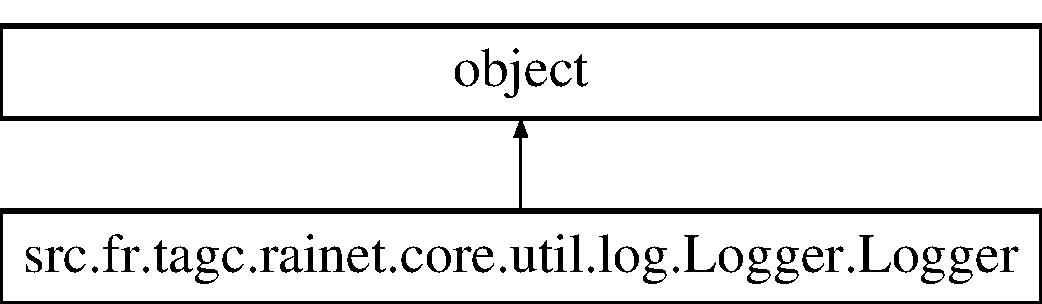
\includegraphics[height=2.000000cm]{classsrc_1_1fr_1_1tagc_1_1rainet_1_1core_1_1util_1_1log_1_1Logger_1_1Logger}
\end{center}
\end{figure}
\subsection*{Public Member Functions}
\begin{DoxyCompactItemize}
\item 
\hypertarget{classsrc_1_1fr_1_1tagc_1_1rainet_1_1core_1_1util_1_1log_1_1Logger_1_1Logger_a65ab4e39e4df0703d277410e73e9efad}{def {\bfseries \-\_\-\-\_\-init\-\_\-\-\_\-}}\label{classsrc_1_1fr_1_1tagc_1_1rainet_1_1core_1_1util_1_1log_1_1Logger_1_1Logger_a65ab4e39e4df0703d277410e73e9efad}

\item 
\hypertarget{classsrc_1_1fr_1_1tagc_1_1rainet_1_1core_1_1util_1_1log_1_1Logger_1_1Logger_ae6c91ee012f5d791a167783d9dad20b8}{def {\bfseries set\-Logger}}\label{classsrc_1_1fr_1_1tagc_1_1rainet_1_1core_1_1util_1_1log_1_1Logger_1_1Logger_ae6c91ee012f5d791a167783d9dad20b8}

\item 
def \hyperlink{classsrc_1_1fr_1_1tagc_1_1rainet_1_1core_1_1util_1_1log_1_1Logger_1_1Logger_a665817e85adba09155cc41ab51b2126e}{set\-\_\-level}
\begin{DoxyCompactList}\small\item\em Set the level of verbosity to the given level. \end{DoxyCompactList}\item 
\hypertarget{classsrc_1_1fr_1_1tagc_1_1rainet_1_1core_1_1util_1_1log_1_1Logger_1_1Logger_a9dd8f1ccdb2a57921439bc7e24cefbc0}{def {\bfseries debug}}\label{classsrc_1_1fr_1_1tagc_1_1rainet_1_1core_1_1util_1_1log_1_1Logger_1_1Logger_a9dd8f1ccdb2a57921439bc7e24cefbc0}

\item 
\hypertarget{classsrc_1_1fr_1_1tagc_1_1rainet_1_1core_1_1util_1_1log_1_1Logger_1_1Logger_a37ddf8f1b8792e56d41b632d7a638fe7}{def {\bfseries info}}\label{classsrc_1_1fr_1_1tagc_1_1rainet_1_1core_1_1util_1_1log_1_1Logger_1_1Logger_a37ddf8f1b8792e56d41b632d7a638fe7}

\item 
\hypertarget{classsrc_1_1fr_1_1tagc_1_1rainet_1_1core_1_1util_1_1log_1_1Logger_1_1Logger_af6797cc05924aef6ea4b55aec61f7172}{def {\bfseries warning}}\label{classsrc_1_1fr_1_1tagc_1_1rainet_1_1core_1_1util_1_1log_1_1Logger_1_1Logger_af6797cc05924aef6ea4b55aec61f7172}

\item 
\hypertarget{classsrc_1_1fr_1_1tagc_1_1rainet_1_1core_1_1util_1_1log_1_1Logger_1_1Logger_a34139260c7bad8c831590715de2f304a}{def {\bfseries error}}\label{classsrc_1_1fr_1_1tagc_1_1rainet_1_1core_1_1util_1_1log_1_1Logger_1_1Logger_a34139260c7bad8c831590715de2f304a}

\item 
\hypertarget{classsrc_1_1fr_1_1tagc_1_1rainet_1_1core_1_1util_1_1log_1_1Logger_1_1Logger_a76d05fc1a93bf272dda497179dbd5f79}{def {\bfseries critical}}\label{classsrc_1_1fr_1_1tagc_1_1rainet_1_1core_1_1util_1_1log_1_1Logger_1_1Logger_a76d05fc1a93bf272dda497179dbd5f79}

\end{DoxyCompactItemize}
\subsection*{Static Public Member Functions}
\begin{DoxyCompactItemize}
\item 
\hypertarget{classsrc_1_1fr_1_1tagc_1_1rainet_1_1core_1_1util_1_1log_1_1Logger_1_1Logger_a3f0abad51db7adca1c39eaa1be8c9fe7}{def {\bfseries get\-\_\-instance}}\label{classsrc_1_1fr_1_1tagc_1_1rainet_1_1core_1_1util_1_1log_1_1Logger_1_1Logger_a3f0abad51db7adca1c39eaa1be8c9fe7}

\end{DoxyCompactItemize}
\subsection*{Public Attributes}
\begin{DoxyCompactItemize}
\item 
\hypertarget{classsrc_1_1fr_1_1tagc_1_1rainet_1_1core_1_1util_1_1log_1_1Logger_1_1Logger_a4602026d1e48039f2ba504e357c095aa}{{\bfseries logg}}\label{classsrc_1_1fr_1_1tagc_1_1rainet_1_1core_1_1util_1_1log_1_1Logger_1_1Logger_a4602026d1e48039f2ba504e357c095aa}

\item 
\hypertarget{classsrc_1_1fr_1_1tagc_1_1rainet_1_1core_1_1util_1_1log_1_1Logger_1_1Logger_ab0f58209e1de80c1f104cacfd1ae54b9}{{\bfseries file\-Handler}}\label{classsrc_1_1fr_1_1tagc_1_1rainet_1_1core_1_1util_1_1log_1_1Logger_1_1Logger_ab0f58209e1de80c1f104cacfd1ae54b9}

\item 
\hypertarget{classsrc_1_1fr_1_1tagc_1_1rainet_1_1core_1_1util_1_1log_1_1Logger_1_1Logger_a4d3ced58e204871da24a3b570edb9c53}{{\bfseries stream\-Handler}}\label{classsrc_1_1fr_1_1tagc_1_1rainet_1_1core_1_1util_1_1log_1_1Logger_1_1Logger_a4d3ced58e204871da24a3b570edb9c53}

\end{DoxyCompactItemize}


\subsection{Detailed Description}
This class is a singleton used to manage logging It contains several method to add log at different level and manage both output to file and standard output. 

\subsection{Member Function Documentation}
\hypertarget{classsrc_1_1fr_1_1tagc_1_1rainet_1_1core_1_1util_1_1log_1_1Logger_1_1Logger_a665817e85adba09155cc41ab51b2126e}{\index{src\-::fr\-::tagc\-::rainet\-::core\-::util\-::log\-::\-Logger\-::\-Logger@{src\-::fr\-::tagc\-::rainet\-::core\-::util\-::log\-::\-Logger\-::\-Logger}!set\-\_\-level@{set\-\_\-level}}
\index{set\-\_\-level@{set\-\_\-level}!src::fr::tagc::rainet::core::util::log::Logger::Logger@{src\-::fr\-::tagc\-::rainet\-::core\-::util\-::log\-::\-Logger\-::\-Logger}}
\subsubsection[{set\-\_\-level}]{\setlength{\rightskip}{0pt plus 5cm}def src.\-fr.\-tagc.\-rainet.\-core.\-util.\-log.\-Logger.\-Logger.\-set\-\_\-level (
\begin{DoxyParamCaption}
\item[{}]{self, }
\item[{}]{level}
\end{DoxyParamCaption}
)}}\label{classsrc_1_1fr_1_1tagc_1_1rainet_1_1core_1_1util_1_1log_1_1Logger_1_1Logger_a665817e85adba09155cc41ab51b2126e}


Set the level of verbosity to the given level. 


\begin{DoxyParams}{Parameters}
{\em level} & \-: string -\/ The level of verbosity \\
\hline
\end{DoxyParams}


The documentation for this class was generated from the following file\-:\begin{DoxyCompactItemize}
\item 
src/fr/tagc/rainet/core/util/log/Logger.\-py\end{DoxyCompactItemize}

\hypertarget{classsrc_1_1core_1_1execution_1_1MakeDatasetRbp_1_1MakeDatasetRbp}{\section{src.\-core.\-execution.\-Make\-Dataset\-Rbp.\-Make\-Dataset\-Rbp Class Reference}
\label{classsrc_1_1core_1_1execution_1_1MakeDatasetRbp_1_1MakeDatasetRbp}\index{src.\-core.\-execution.\-Make\-Dataset\-Rbp.\-Make\-Dataset\-Rbp@{src.\-core.\-execution.\-Make\-Dataset\-Rbp.\-Make\-Dataset\-Rbp}}
}
\subsection*{Public Member Functions}
\begin{DoxyCompactItemize}
\item 
\hypertarget{classsrc_1_1core_1_1execution_1_1MakeDatasetRbp_1_1MakeDatasetRbp_a41fccbe107fd4affee8d04b7c4476dae}{def {\bfseries comparison\-\_\-dataset}}\label{classsrc_1_1core_1_1execution_1_1MakeDatasetRbp_1_1MakeDatasetRbp_a41fccbe107fd4affee8d04b7c4476dae}

\item 
\hypertarget{classsrc_1_1core_1_1execution_1_1MakeDatasetRbp_1_1MakeDatasetRbp_a4f0dae78969501e102ff7d141dd0e4a2}{def {\bfseries creation\-\_\-list}}\label{classsrc_1_1core_1_1execution_1_1MakeDatasetRbp_1_1MakeDatasetRbp_a4f0dae78969501e102ff7d141dd0e4a2}

\item 
\hypertarget{classsrc_1_1core_1_1execution_1_1MakeDatasetRbp_1_1MakeDatasetRbp_ac0de547a0ac56c8dfa4a30df453b7c1f}{def {\bfseries connection\-\_\-to\-\_\-ensembl}}\label{classsrc_1_1core_1_1execution_1_1MakeDatasetRbp_1_1MakeDatasetRbp_ac0de547a0ac56c8dfa4a30df453b7c1f}

\item 
\hypertarget{classsrc_1_1core_1_1execution_1_1MakeDatasetRbp_1_1MakeDatasetRbp_a1b8e836be9cb0ee2ddc598a4ffda57cc}{def {\bfseries dictionary\-\_\-identifier}}\label{classsrc_1_1core_1_1execution_1_1MakeDatasetRbp_1_1MakeDatasetRbp_a1b8e836be9cb0ee2ddc598a4ffda57cc}

\item 
\hypertarget{classsrc_1_1core_1_1execution_1_1MakeDatasetRbp_1_1MakeDatasetRbp_aa33e4ce52dd1f1c29b129f07fa0f06d5}{def {\bfseries longest\-\_\-sequence}}\label{classsrc_1_1core_1_1execution_1_1MakeDatasetRbp_1_1MakeDatasetRbp_aa33e4ce52dd1f1c29b129f07fa0f06d5}

\item 
\hypertarget{classsrc_1_1core_1_1execution_1_1MakeDatasetRbp_1_1MakeDatasetRbp_a0525c07bb38cb39454a123caff306c4c}{def {\bfseries isoform\-\_\-sequences}}\label{classsrc_1_1core_1_1execution_1_1MakeDatasetRbp_1_1MakeDatasetRbp_a0525c07bb38cb39454a123caff306c4c}

\item 
\hypertarget{classsrc_1_1core_1_1execution_1_1MakeDatasetRbp_1_1MakeDatasetRbp_a92489d16d6f9352b52730b26b146a5b8}{def {\bfseries merger\-\_\-sequences}}\label{classsrc_1_1core_1_1execution_1_1MakeDatasetRbp_1_1MakeDatasetRbp_a92489d16d6f9352b52730b26b146a5b8}

\item 
\hypertarget{classsrc_1_1core_1_1execution_1_1MakeDatasetRbp_1_1MakeDatasetRbp_a039e12a82cd9269ad18e25d267f1c0a9}{def {\bfseries delet\-\_\-append\-\_\-file}}\label{classsrc_1_1core_1_1execution_1_1MakeDatasetRbp_1_1MakeDatasetRbp_a039e12a82cd9269ad18e25d267f1c0a9}

\end{DoxyCompactItemize}
\subsection*{Static Public Member Functions}
\begin{DoxyCompactItemize}
\item 
\hypertarget{classsrc_1_1core_1_1execution_1_1MakeDatasetRbp_1_1MakeDatasetRbp_a473df3fd137882a894070e933e308230}{def {\bfseries whole\-\_\-procedure}}\label{classsrc_1_1core_1_1execution_1_1MakeDatasetRbp_1_1MakeDatasetRbp_a473df3fd137882a894070e933e308230}

\end{DoxyCompactItemize}
\subsection*{Public Attributes}
\begin{DoxyCompactItemize}
\item 
\hypertarget{classsrc_1_1core_1_1execution_1_1MakeDatasetRbp_1_1MakeDatasetRbp_a193b7107f4a2d7cbe04864b9c2391db6}{{\bfseries dataset\-\_\-input\-\_\-path}}\label{classsrc_1_1core_1_1execution_1_1MakeDatasetRbp_1_1MakeDatasetRbp_a193b7107f4a2d7cbe04864b9c2391db6}

\item 
\hypertarget{classsrc_1_1core_1_1execution_1_1MakeDatasetRbp_1_1MakeDatasetRbp_a020d0251c520c6b074a040613ccce389}{{\bfseries dataset\-\_\-1\-\_\-file}}\label{classsrc_1_1core_1_1execution_1_1MakeDatasetRbp_1_1MakeDatasetRbp_a020d0251c520c6b074a040613ccce389}

\item 
\hypertarget{classsrc_1_1core_1_1execution_1_1MakeDatasetRbp_1_1MakeDatasetRbp_aea25fc9befde71d00305d45590f32cca}{{\bfseries dataset\-\_\-2\-\_\-file}}\label{classsrc_1_1core_1_1execution_1_1MakeDatasetRbp_1_1MakeDatasetRbp_aea25fc9befde71d00305d45590f32cca}

\item 
\hypertarget{classsrc_1_1core_1_1execution_1_1MakeDatasetRbp_1_1MakeDatasetRbp_a171856a89faf4a45d03245840f2415fe}{{\bfseries dataset\-\_\-1\-\_\-index\-\_\-col}}\label{classsrc_1_1core_1_1execution_1_1MakeDatasetRbp_1_1MakeDatasetRbp_a171856a89faf4a45d03245840f2415fe}

\item 
\hypertarget{classsrc_1_1core_1_1execution_1_1MakeDatasetRbp_1_1MakeDatasetRbp_a01fb942288e87904829fcb2a191a01fb}{{\bfseries dataset\-\_\-2\-\_\-index\-\_\-col}}\label{classsrc_1_1core_1_1execution_1_1MakeDatasetRbp_1_1MakeDatasetRbp_a01fb942288e87904829fcb2a191a01fb}

\item 
\hypertarget{classsrc_1_1core_1_1execution_1_1MakeDatasetRbp_1_1MakeDatasetRbp_aeb89d952c2d199061e361d72896fdb25}{{\bfseries dataset\-\_\-output}}\label{classsrc_1_1core_1_1execution_1_1MakeDatasetRbp_1_1MakeDatasetRbp_aeb89d952c2d199061e361d72896fdb25}

\item 
\hypertarget{classsrc_1_1core_1_1execution_1_1MakeDatasetRbp_1_1MakeDatasetRbp_a665358ce47f2f8ed10cb524d238ebcdb}{{\bfseries dataset\-\_\-1\-\_\-length}}\label{classsrc_1_1core_1_1execution_1_1MakeDatasetRbp_1_1MakeDatasetRbp_a665358ce47f2f8ed10cb524d238ebcdb}

\item 
\hypertarget{classsrc_1_1core_1_1execution_1_1MakeDatasetRbp_1_1MakeDatasetRbp_a04aba2c69cd214f1810b358f5fc01bb6}{{\bfseries dataset\-\_\-2\-\_\-length}}\label{classsrc_1_1core_1_1execution_1_1MakeDatasetRbp_1_1MakeDatasetRbp_a04aba2c69cd214f1810b358f5fc01bb6}

\item 
\hypertarget{classsrc_1_1core_1_1execution_1_1MakeDatasetRbp_1_1MakeDatasetRbp_a6e899e477f2cda18cfaa436b9ea29f78}{{\bfseries index\-\_\-col}}\label{classsrc_1_1core_1_1execution_1_1MakeDatasetRbp_1_1MakeDatasetRbp_a6e899e477f2cda18cfaa436b9ea29f78}

\item 
\hypertarget{classsrc_1_1core_1_1execution_1_1MakeDatasetRbp_1_1MakeDatasetRbp_a2c23deb65346a5a9dcb912d5846b8435}{{\bfseries dataset\-\_\-length}}\label{classsrc_1_1core_1_1execution_1_1MakeDatasetRbp_1_1MakeDatasetRbp_a2c23deb65346a5a9dcb912d5846b8435}

\item 
\hypertarget{classsrc_1_1core_1_1execution_1_1MakeDatasetRbp_1_1MakeDatasetRbp_a51ab17198bad0a1521a4e56d97b52e31}{{\bfseries path\-\_\-home}}\label{classsrc_1_1core_1_1execution_1_1MakeDatasetRbp_1_1MakeDatasetRbp_a51ab17198bad0a1521a4e56d97b52e31}

\item 
\hypertarget{classsrc_1_1core_1_1execution_1_1MakeDatasetRbp_1_1MakeDatasetRbp_ac3da1c27a4df2f599bf22b0d0bdf15e5}{{\bfseries file\-\_\-dataset\-\_\-1}}\label{classsrc_1_1core_1_1execution_1_1MakeDatasetRbp_1_1MakeDatasetRbp_ac3da1c27a4df2f599bf22b0d0bdf15e5}

\item 
\hypertarget{classsrc_1_1core_1_1execution_1_1MakeDatasetRbp_1_1MakeDatasetRbp_a954145cefa9d7226452c741ccd214eed}{{\bfseries gene\-\_\-index\-\_\-col}}\label{classsrc_1_1core_1_1execution_1_1MakeDatasetRbp_1_1MakeDatasetRbp_a954145cefa9d7226452c741ccd214eed}

\item 
\hypertarget{classsrc_1_1core_1_1execution_1_1MakeDatasetRbp_1_1MakeDatasetRbp_aedaccb70edf6641c35aca8dfd807865c}{{\bfseries protein\-\_\-index\-\_\-col}}\label{classsrc_1_1core_1_1execution_1_1MakeDatasetRbp_1_1MakeDatasetRbp_aedaccb70edf6641c35aca8dfd807865c}

\item 
\hypertarget{classsrc_1_1core_1_1execution_1_1MakeDatasetRbp_1_1MakeDatasetRbp_a523e3857c0a19d34cebecc1f508137a0}{{\bfseries list\-\_\-gene\-\_\-dataset\-\_\-1}}\label{classsrc_1_1core_1_1execution_1_1MakeDatasetRbp_1_1MakeDatasetRbp_a523e3857c0a19d34cebecc1f508137a0}

\item 
\hypertarget{classsrc_1_1core_1_1execution_1_1MakeDatasetRbp_1_1MakeDatasetRbp_ac4297cb83b5dd3adb2895a8bc6778fad}{{\bfseries list\-\_\-protein\-\_\-dataset\-\_\-1}}\label{classsrc_1_1core_1_1execution_1_1MakeDatasetRbp_1_1MakeDatasetRbp_ac4297cb83b5dd3adb2895a8bc6778fad}

\item 
\hypertarget{classsrc_1_1core_1_1execution_1_1MakeDatasetRbp_1_1MakeDatasetRbp_a70ebd85295682d7a68502c90f95d2794}{{\bfseries path\-\_\-gene\-\_\-dataset\-\_\-1}}\label{classsrc_1_1core_1_1execution_1_1MakeDatasetRbp_1_1MakeDatasetRbp_a70ebd85295682d7a68502c90f95d2794}

\item 
\hypertarget{classsrc_1_1core_1_1execution_1_1MakeDatasetRbp_1_1MakeDatasetRbp_abd36e777d48e1e217b365722b41b3fdb}{{\bfseries path\-\_\-protein\-\_\-dataset\-\_\-1}}\label{classsrc_1_1core_1_1execution_1_1MakeDatasetRbp_1_1MakeDatasetRbp_abd36e777d48e1e217b365722b41b3fdb}

\item 
\hypertarget{classsrc_1_1core_1_1execution_1_1MakeDatasetRbp_1_1MakeDatasetRbp_a2253dd8aaf94ee12c2070c3a91a86b8a}{{\bfseries path\-\_\-dataset\-\_\-1}}\label{classsrc_1_1core_1_1execution_1_1MakeDatasetRbp_1_1MakeDatasetRbp_a2253dd8aaf94ee12c2070c3a91a86b8a}

\item 
\hypertarget{classsrc_1_1core_1_1execution_1_1MakeDatasetRbp_1_1MakeDatasetRbp_ab5c34bfb51dedb19be6c4f27183ef341}{{\bfseries list\-\_\-path}}\label{classsrc_1_1core_1_1execution_1_1MakeDatasetRbp_1_1MakeDatasetRbp_ab5c34bfb51dedb19be6c4f27183ef341}

\item 
\hypertarget{classsrc_1_1core_1_1execution_1_1MakeDatasetRbp_1_1MakeDatasetRbp_ab8e481b52f3d7bf62c81a8cf44ff1b6e}{{\bfseries gene\-\_\-list\-\_\-1}}\label{classsrc_1_1core_1_1execution_1_1MakeDatasetRbp_1_1MakeDatasetRbp_ab8e481b52f3d7bf62c81a8cf44ff1b6e}

\item 
\hypertarget{classsrc_1_1core_1_1execution_1_1MakeDatasetRbp_1_1MakeDatasetRbp_a529c6ce05a03e158645c81313b14d47e}{{\bfseries protein\-\_\-list}}\label{classsrc_1_1core_1_1execution_1_1MakeDatasetRbp_1_1MakeDatasetRbp_a529c6ce05a03e158645c81313b14d47e}

\item 
\hypertarget{classsrc_1_1core_1_1execution_1_1MakeDatasetRbp_1_1MakeDatasetRbp_acfe474f85fd20a668aef5d273f0ec1f2}{{\bfseries ensembl\-\_\-gene\-\_\-list\-\_\-1\-\_\-path}}\label{classsrc_1_1core_1_1execution_1_1MakeDatasetRbp_1_1MakeDatasetRbp_acfe474f85fd20a668aef5d273f0ec1f2}

\item 
\hypertarget{classsrc_1_1core_1_1execution_1_1MakeDatasetRbp_1_1MakeDatasetRbp_a64e2ab32cfcca8ae2077acc5498c8dca}{{\bfseries ensembl\-\_\-protein\-\_\-list\-\_\-1\-\_\-path}}\label{classsrc_1_1core_1_1execution_1_1MakeDatasetRbp_1_1MakeDatasetRbp_a64e2ab32cfcca8ae2077acc5498c8dca}

\item 
\hypertarget{classsrc_1_1core_1_1execution_1_1MakeDatasetRbp_1_1MakeDatasetRbp_a61d313279561855e9cb0a297cabc3d71}{{\bfseries type\-\_\-query1\-\_\-ensembl}}\label{classsrc_1_1core_1_1execution_1_1MakeDatasetRbp_1_1MakeDatasetRbp_a61d313279561855e9cb0a297cabc3d71}

\item 
\hypertarget{classsrc_1_1core_1_1execution_1_1MakeDatasetRbp_1_1MakeDatasetRbp_a7d45cf13f2ce821c7fbe7bacac342d6d}{{\bfseries ensembl\-\_\-path\-\_\-output}}\label{classsrc_1_1core_1_1execution_1_1MakeDatasetRbp_1_1MakeDatasetRbp_a7d45cf13f2ce821c7fbe7bacac342d6d}

\item 
\hypertarget{classsrc_1_1core_1_1execution_1_1MakeDatasetRbp_1_1MakeDatasetRbp_a0b3a115e3b339761bc472562f42b7a8b}{{\bfseries ensembl\-\_\-output\-\_\-dataset1}}\label{classsrc_1_1core_1_1execution_1_1MakeDatasetRbp_1_1MakeDatasetRbp_a0b3a115e3b339761bc472562f42b7a8b}

\item 
\hypertarget{classsrc_1_1core_1_1execution_1_1MakeDatasetRbp_1_1MakeDatasetRbp_a90f873be2cb21796584e60743907e27e}{{\bfseries ensembl\-\_\-input\-\_\-list\-\_\-2}}\label{classsrc_1_1core_1_1execution_1_1MakeDatasetRbp_1_1MakeDatasetRbp_a90f873be2cb21796584e60743907e27e}

\item 
\hypertarget{classsrc_1_1core_1_1execution_1_1MakeDatasetRbp_1_1MakeDatasetRbp_a1a12dbb47bd49fc731f29315741880b1}{{\bfseries gene\-\_\-list\-\_\-2}}\label{classsrc_1_1core_1_1execution_1_1MakeDatasetRbp_1_1MakeDatasetRbp_a1a12dbb47bd49fc731f29315741880b1}

\item 
\hypertarget{classsrc_1_1core_1_1execution_1_1MakeDatasetRbp_1_1MakeDatasetRbp_a47812470682747b31e37e987f7a3f880}{{\bfseries ensembl\-\_\-gene\-\_\-list\-\_\-2\-\_\-path}}\label{classsrc_1_1core_1_1execution_1_1MakeDatasetRbp_1_1MakeDatasetRbp_a47812470682747b31e37e987f7a3f880}

\item 
\hypertarget{classsrc_1_1core_1_1execution_1_1MakeDatasetRbp_1_1MakeDatasetRbp_a5e394764b49f741394cad9a01c65f8aa}{{\bfseries type\-\_\-query2\-\_\-ensembl}}\label{classsrc_1_1core_1_1execution_1_1MakeDatasetRbp_1_1MakeDatasetRbp_a5e394764b49f741394cad9a01c65f8aa}

\item 
\hypertarget{classsrc_1_1core_1_1execution_1_1MakeDatasetRbp_1_1MakeDatasetRbp_a93d0d46d29aef896cd4bec487f7c0512}{{\bfseries ensembl\-\_\-output\-\_\-dataset2}}\label{classsrc_1_1core_1_1execution_1_1MakeDatasetRbp_1_1MakeDatasetRbp_a93d0d46d29aef896cd4bec487f7c0512}

\item 
\hypertarget{classsrc_1_1core_1_1execution_1_1MakeDatasetRbp_1_1MakeDatasetRbp_aa8c582dcb25006acbc2b33a332cbb2ef}{{\bfseries dictionary\-\_\-output}}\label{classsrc_1_1core_1_1execution_1_1MakeDatasetRbp_1_1MakeDatasetRbp_aa8c582dcb25006acbc2b33a332cbb2ef}

\item 
\hypertarget{classsrc_1_1core_1_1execution_1_1MakeDatasetRbp_1_1MakeDatasetRbp_aef2b736393f2662cf437d5ce94debf89}{{\bfseries dictionary\-\_\-namefile}}\label{classsrc_1_1core_1_1execution_1_1MakeDatasetRbp_1_1MakeDatasetRbp_aef2b736393f2662cf437d5ce94debf89}

\item 
\hypertarget{classsrc_1_1core_1_1execution_1_1MakeDatasetRbp_1_1MakeDatasetRbp_a97f85759f35ab7807f129fe383e16bbc}{{\bfseries path\-\_\-sequences}}\label{classsrc_1_1core_1_1execution_1_1MakeDatasetRbp_1_1MakeDatasetRbp_a97f85759f35ab7807f129fe383e16bbc}

\item 
\hypertarget{classsrc_1_1core_1_1execution_1_1MakeDatasetRbp_1_1MakeDatasetRbp_aaa500769371928ec8240e8e97917d45e}{{\bfseries file\-\_\-sequences}}\label{classsrc_1_1core_1_1execution_1_1MakeDatasetRbp_1_1MakeDatasetRbp_aaa500769371928ec8240e8e97917d45e}

\item 
\hypertarget{classsrc_1_1core_1_1execution_1_1MakeDatasetRbp_1_1MakeDatasetRbp_a3a74b95a139bdd45a83ddd3ca3522f33}{{\bfseries path\-\_\-dictionary\-\_\-identifier}}\label{classsrc_1_1core_1_1execution_1_1MakeDatasetRbp_1_1MakeDatasetRbp_a3a74b95a139bdd45a83ddd3ca3522f33}

\item 
\hypertarget{classsrc_1_1core_1_1execution_1_1MakeDatasetRbp_1_1MakeDatasetRbp_a962e1755f1c6763a748c1b23d1fdc875}{{\bfseries file\-\_\-dictionary}}\label{classsrc_1_1core_1_1execution_1_1MakeDatasetRbp_1_1MakeDatasetRbp_a962e1755f1c6763a748c1b23d1fdc875}

\item 
\hypertarget{classsrc_1_1core_1_1execution_1_1MakeDatasetRbp_1_1MakeDatasetRbp_a72c464cf22d2a530e54dacbba5d9c0d8}{{\bfseries path\-\_\-output\-\_\-longest}}\label{classsrc_1_1core_1_1execution_1_1MakeDatasetRbp_1_1MakeDatasetRbp_a72c464cf22d2a530e54dacbba5d9c0d8}

\item 
\hypertarget{classsrc_1_1core_1_1execution_1_1MakeDatasetRbp_1_1MakeDatasetRbp_adaf351378531bdc20602c8945142556f}{{\bfseries path\-\_\-file\-\_\-longest}}\label{classsrc_1_1core_1_1execution_1_1MakeDatasetRbp_1_1MakeDatasetRbp_adaf351378531bdc20602c8945142556f}

\item 
\hypertarget{classsrc_1_1core_1_1execution_1_1MakeDatasetRbp_1_1MakeDatasetRbp_a568e0a515c5c908203b54b0b99db4379}{{\bfseries path\-\_\-file\-\_\-isoform}}\label{classsrc_1_1core_1_1execution_1_1MakeDatasetRbp_1_1MakeDatasetRbp_a568e0a515c5c908203b54b0b99db4379}

\item 
\hypertarget{classsrc_1_1core_1_1execution_1_1MakeDatasetRbp_1_1MakeDatasetRbp_a1e2bf17ac754a95bad674e6bfdf5d95c}{{\bfseries path\-\_\-file\-\_\-selected\-\_\-isoform}}\label{classsrc_1_1core_1_1execution_1_1MakeDatasetRbp_1_1MakeDatasetRbp_a1e2bf17ac754a95bad674e6bfdf5d95c}

\item 
\hypertarget{classsrc_1_1core_1_1execution_1_1MakeDatasetRbp_1_1MakeDatasetRbp_a74cb0ba5eb089ad57e22661d500b10e4}{{\bfseries headers}}\label{classsrc_1_1core_1_1execution_1_1MakeDatasetRbp_1_1MakeDatasetRbp_a74cb0ba5eb089ad57e22661d500b10e4}

\item 
\hypertarget{classsrc_1_1core_1_1execution_1_1MakeDatasetRbp_1_1MakeDatasetRbp_a5629f5ee71866009afc2ac198604a42f}{{\bfseries file\-\_\-random\-\_\-seq}}\label{classsrc_1_1core_1_1execution_1_1MakeDatasetRbp_1_1MakeDatasetRbp_a5629f5ee71866009afc2ac198604a42f}

\item 
\hypertarget{classsrc_1_1core_1_1execution_1_1MakeDatasetRbp_1_1MakeDatasetRbp_a22b9931ea48f3861b079462900f7a885}{{\bfseries path\-\_\-input\-\_\-longest}}\label{classsrc_1_1core_1_1execution_1_1MakeDatasetRbp_1_1MakeDatasetRbp_a22b9931ea48f3861b079462900f7a885}

\item 
\hypertarget{classsrc_1_1core_1_1execution_1_1MakeDatasetRbp_1_1MakeDatasetRbp_ace0025b0eed61ee6ff91c9f949a7c987}{{\bfseries path\-\_\-output\-\_\-seq}}\label{classsrc_1_1core_1_1execution_1_1MakeDatasetRbp_1_1MakeDatasetRbp_ace0025b0eed61ee6ff91c9f949a7c987}

\item 
\hypertarget{classsrc_1_1core_1_1execution_1_1MakeDatasetRbp_1_1MakeDatasetRbp_a1c9ea73fe4c75ea24b10a90afedba019}{{\bfseries path\-\_\-file\-\_\-seq\-\_\-dataset\-\_\-2}}\label{classsrc_1_1core_1_1execution_1_1MakeDatasetRbp_1_1MakeDatasetRbp_a1c9ea73fe4c75ea24b10a90afedba019}

\item 
\hypertarget{classsrc_1_1core_1_1execution_1_1MakeDatasetRbp_1_1MakeDatasetRbp_aab67d98c53f5d84db1cb32f7bebdbab5}{{\bfseries path\-\_\-input\-\_\-seq\-\_\-dataset1}}\label{classsrc_1_1core_1_1execution_1_1MakeDatasetRbp_1_1MakeDatasetRbp_aab67d98c53f5d84db1cb32f7bebdbab5}

\item 
\hypertarget{classsrc_1_1core_1_1execution_1_1MakeDatasetRbp_1_1MakeDatasetRbp_a62f96a3b13f1bd9f94038ba6ee59c300}{{\bfseries path\-\_\-file\-\_\-dataset1}}\label{classsrc_1_1core_1_1execution_1_1MakeDatasetRbp_1_1MakeDatasetRbp_a62f96a3b13f1bd9f94038ba6ee59c300}

\item 
\hypertarget{classsrc_1_1core_1_1execution_1_1MakeDatasetRbp_1_1MakeDatasetRbp_a5f5e48bd6e1693ad5dc279410952d315}{{\bfseries path\-\_\-file\-\_\-dataset12}}\label{classsrc_1_1core_1_1execution_1_1MakeDatasetRbp_1_1MakeDatasetRbp_a5f5e48bd6e1693ad5dc279410952d315}

\item 
\hypertarget{classsrc_1_1core_1_1execution_1_1MakeDatasetRbp_1_1MakeDatasetRbp_a76d407a18d5319a28710ecf4b5fba9de}{{\bfseries path\-\_\-input\-\_\-original\-\_\-file}}\label{classsrc_1_1core_1_1execution_1_1MakeDatasetRbp_1_1MakeDatasetRbp_a76d407a18d5319a28710ecf4b5fba9de}

\item 
\hypertarget{classsrc_1_1core_1_1execution_1_1MakeDatasetRbp_1_1MakeDatasetRbp_a5dcc3c7009a0f746e6315d579b301de1}{{\bfseries original\-\_\-file}}\label{classsrc_1_1core_1_1execution_1_1MakeDatasetRbp_1_1MakeDatasetRbp_a5dcc3c7009a0f746e6315d579b301de1}

\item 
\hypertarget{classsrc_1_1core_1_1execution_1_1MakeDatasetRbp_1_1MakeDatasetRbp_ab04d03704a46e410937cf40e029baccb}{{\bfseries del\-\_\-ensembl\-\_\-input}}\label{classsrc_1_1core_1_1execution_1_1MakeDatasetRbp_1_1MakeDatasetRbp_ab04d03704a46e410937cf40e029baccb}

\item 
\hypertarget{classsrc_1_1core_1_1execution_1_1MakeDatasetRbp_1_1MakeDatasetRbp_a51783928edb8ae964a4ac9d0040b4d31}{{\bfseries del\-\_\-ensembl\-\_\-file1}}\label{classsrc_1_1core_1_1execution_1_1MakeDatasetRbp_1_1MakeDatasetRbp_a51783928edb8ae964a4ac9d0040b4d31}

\item 
\hypertarget{classsrc_1_1core_1_1execution_1_1MakeDatasetRbp_1_1MakeDatasetRbp_a6e43c118e8e76fa076899096d44fe2f9}{{\bfseries del\-\_\-ensembl\-\_\-file2}}\label{classsrc_1_1core_1_1execution_1_1MakeDatasetRbp_1_1MakeDatasetRbp_a6e43c118e8e76fa076899096d44fe2f9}

\item 
\hypertarget{classsrc_1_1core_1_1execution_1_1MakeDatasetRbp_1_1MakeDatasetRbp_af2f813052f61b6fab9eba62cf2b8be35}{{\bfseries del\-\_\-longest\-\_\-input}}\label{classsrc_1_1core_1_1execution_1_1MakeDatasetRbp_1_1MakeDatasetRbp_af2f813052f61b6fab9eba62cf2b8be35}

\item 
\hypertarget{classsrc_1_1core_1_1execution_1_1MakeDatasetRbp_1_1MakeDatasetRbp_a6ffe1c78bcf4e091950887a99899a118}{{\bfseries del\-\_\-longest\-\_\-file}}\label{classsrc_1_1core_1_1execution_1_1MakeDatasetRbp_1_1MakeDatasetRbp_a6ffe1c78bcf4e091950887a99899a118}

\item 
\hypertarget{classsrc_1_1core_1_1execution_1_1MakeDatasetRbp_1_1MakeDatasetRbp_ab30e9f0c34901dbaf19a80744c33a4ed}{{\bfseries del\-\_\-isoform\-\_\-file}}\label{classsrc_1_1core_1_1execution_1_1MakeDatasetRbp_1_1MakeDatasetRbp_ab30e9f0c34901dbaf19a80744c33a4ed}

\item 
\hypertarget{classsrc_1_1core_1_1execution_1_1MakeDatasetRbp_1_1MakeDatasetRbp_a3fd8eb5d78c1b4391a44204cafa1af8c}{{\bfseries del\-\_\-random\-\_\-isoform\-\_\-file}}\label{classsrc_1_1core_1_1execution_1_1MakeDatasetRbp_1_1MakeDatasetRbp_a3fd8eb5d78c1b4391a44204cafa1af8c}

\item 
\hypertarget{classsrc_1_1core_1_1execution_1_1MakeDatasetRbp_1_1MakeDatasetRbp_a8081de774ec5b81c57a7553a08501e94}{{\bfseries del\-\_\-fusion\-\_\-path}}\label{classsrc_1_1core_1_1execution_1_1MakeDatasetRbp_1_1MakeDatasetRbp_a8081de774ec5b81c57a7553a08501e94}

\item 
\hypertarget{classsrc_1_1core_1_1execution_1_1MakeDatasetRbp_1_1MakeDatasetRbp_a3e7c2e937161000ed16e109fa75f5948}{{\bfseries del\-\_\-fusion\-\_\-file\-\_\-longest}}\label{classsrc_1_1core_1_1execution_1_1MakeDatasetRbp_1_1MakeDatasetRbp_a3e7c2e937161000ed16e109fa75f5948}

\item 
\hypertarget{classsrc_1_1core_1_1execution_1_1MakeDatasetRbp_1_1MakeDatasetRbp_a6623920d27f5bf02a65df2fcd348c5ab}{{\bfseries del\-\_\-fusion\-\_\-file\-\_\-dataset12}}\label{classsrc_1_1core_1_1execution_1_1MakeDatasetRbp_1_1MakeDatasetRbp_a6623920d27f5bf02a65df2fcd348c5ab}

\end{DoxyCompactItemize}


The documentation for this class was generated from the following file\-:\begin{DoxyCompactItemize}
\item 
rbp-\/motif/src/core/execution/Make\-Dataset\-Rbp.\-py\end{DoxyCompactItemize}

\hypertarget{classsrc_1_1core_1_1execution_1_1MotifsAnalysis_1_1MotifsAnalysis}{\section{src.\-core.\-execution.\-Motifs\-Analysis.\-Motifs\-Analysis Class Reference}
\label{classsrc_1_1core_1_1execution_1_1MotifsAnalysis_1_1MotifsAnalysis}\index{src.\-core.\-execution.\-Motifs\-Analysis.\-Motifs\-Analysis@{src.\-core.\-execution.\-Motifs\-Analysis.\-Motifs\-Analysis}}
}
\subsection*{Public Member Functions}
\begin{DoxyCompactItemize}
\item 
\hypertarget{classsrc_1_1core_1_1execution_1_1MotifsAnalysis_1_1MotifsAnalysis_a918e4875994c24e1a41534a881148df1}{def {\bfseries \-\_\-\-\_\-init\-\_\-\-\_\-}}\label{classsrc_1_1core_1_1execution_1_1MotifsAnalysis_1_1MotifsAnalysis_a918e4875994c24e1a41534a881148df1}

\item 
\hypertarget{classsrc_1_1core_1_1execution_1_1MotifsAnalysis_1_1MotifsAnalysis_a0bdcb665161e1e606c57464c8b67b702}{def {\bfseries iupred\-\_\-motifs}}\label{classsrc_1_1core_1_1execution_1_1MotifsAnalysis_1_1MotifsAnalysis_a0bdcb665161e1e606c57464c8b67b702}

\item 
\hypertarget{classsrc_1_1core_1_1execution_1_1MotifsAnalysis_1_1MotifsAnalysis_a89365f54ac0fa8e29b4cea3c0889b7ab}{def {\bfseries anchor\-\_\-motifs}}\label{classsrc_1_1core_1_1execution_1_1MotifsAnalysis_1_1MotifsAnalysis_a89365f54ac0fa8e29b4cea3c0889b7ab}

\item 
\hypertarget{classsrc_1_1core_1_1execution_1_1MotifsAnalysis_1_1MotifsAnalysis_aa177d2a61787792fd7e384180bd8feea}{def {\bfseries disordp\-\_\-motifs}}\label{classsrc_1_1core_1_1execution_1_1MotifsAnalysis_1_1MotifsAnalysis_aa177d2a61787792fd7e384180bd8feea}

\end{DoxyCompactItemize}
\subsection*{Static Public Member Functions}
\begin{DoxyCompactItemize}
\item 
\hypertarget{classsrc_1_1core_1_1execution_1_1MotifsAnalysis_1_1MotifsAnalysis_a3ed00e17082faead8831fe7e579699cc}{def {\bfseries whole\-\_\-procedure}}\label{classsrc_1_1core_1_1execution_1_1MotifsAnalysis_1_1MotifsAnalysis_a3ed00e17082faead8831fe7e579699cc}

\end{DoxyCompactItemize}
\subsection*{Public Attributes}
\begin{DoxyCompactItemize}
\item 
\hypertarget{classsrc_1_1core_1_1execution_1_1MotifsAnalysis_1_1MotifsAnalysis_a270ea66ef22270bb8dc3dccddc093393}{{\bfseries path\-\_\-home}}\label{classsrc_1_1core_1_1execution_1_1MotifsAnalysis_1_1MotifsAnalysis_a270ea66ef22270bb8dc3dccddc093393}

\item 
\hypertarget{classsrc_1_1core_1_1execution_1_1MotifsAnalysis_1_1MotifsAnalysis_a6d198d0c2f7d484c0b0a0bdb2e5eaada}{{\bfseries protein\-\_\-list\-\_\-file}}\label{classsrc_1_1core_1_1execution_1_1MotifsAnalysis_1_1MotifsAnalysis_a6d198d0c2f7d484c0b0a0bdb2e5eaada}

\item 
\hypertarget{classsrc_1_1core_1_1execution_1_1MotifsAnalysis_1_1MotifsAnalysis_af405d8b231569b6ad236e21d098af69b}{{\bfseries protein\-\_\-list}}\label{classsrc_1_1core_1_1execution_1_1MotifsAnalysis_1_1MotifsAnalysis_af405d8b231569b6ad236e21d098af69b}

\item 
\hypertarget{classsrc_1_1core_1_1execution_1_1MotifsAnalysis_1_1MotifsAnalysis_aff3aef3cb876455488f148c6d2d60609}{{\bfseries motif\-\_\-folder}}\label{classsrc_1_1core_1_1execution_1_1MotifsAnalysis_1_1MotifsAnalysis_aff3aef3cb876455488f148c6d2d60609}

\item 
\hypertarget{classsrc_1_1core_1_1execution_1_1MotifsAnalysis_1_1MotifsAnalysis_a33e404cfd785978a89623936d4b38562}{{\bfseries domain\-\_\-region\-\_\-file}}\label{classsrc_1_1core_1_1execution_1_1MotifsAnalysis_1_1MotifsAnalysis_a33e404cfd785978a89623936d4b38562}

\item 
\hypertarget{classsrc_1_1core_1_1execution_1_1MotifsAnalysis_1_1MotifsAnalysis_a90ef1fe5970cde451df2392c5699af1b}{{\bfseries iupred\-\_\-folder}}\label{classsrc_1_1core_1_1execution_1_1MotifsAnalysis_1_1MotifsAnalysis_a90ef1fe5970cde451df2392c5699af1b}

\item 
\hypertarget{classsrc_1_1core_1_1execution_1_1MotifsAnalysis_1_1MotifsAnalysis_ac38f987cab4bbf4f6f6ed3d79b3d8759}{{\bfseries threshold\-\_\-1}}\label{classsrc_1_1core_1_1execution_1_1MotifsAnalysis_1_1MotifsAnalysis_ac38f987cab4bbf4f6f6ed3d79b3d8759}

\item 
\hypertarget{classsrc_1_1core_1_1execution_1_1MotifsAnalysis_1_1MotifsAnalysis_abc5cbe67b9845b781f2f9874d979103b}{{\bfseries output\-\_\-folder\-\_\-1}}\label{classsrc_1_1core_1_1execution_1_1MotifsAnalysis_1_1MotifsAnalysis_abc5cbe67b9845b781f2f9874d979103b}

\item 
\hypertarget{classsrc_1_1core_1_1execution_1_1MotifsAnalysis_1_1MotifsAnalysis_a414b5c32c2f94f58b0008d5b721722c5}{{\bfseries threshold\-\_\-2}}\label{classsrc_1_1core_1_1execution_1_1MotifsAnalysis_1_1MotifsAnalysis_a414b5c32c2f94f58b0008d5b721722c5}

\item 
\hypertarget{classsrc_1_1core_1_1execution_1_1MotifsAnalysis_1_1MotifsAnalysis_a0f512cfa4fb37e3df75c0dbacef970e6}{{\bfseries output\-\_\-folder\-\_\-2}}\label{classsrc_1_1core_1_1execution_1_1MotifsAnalysis_1_1MotifsAnalysis_a0f512cfa4fb37e3df75c0dbacef970e6}

\item 
\hypertarget{classsrc_1_1core_1_1execution_1_1MotifsAnalysis_1_1MotifsAnalysis_adc404243a06030af2244276f5d4aedb5}{{\bfseries anchor\-\_\-folder}}\label{classsrc_1_1core_1_1execution_1_1MotifsAnalysis_1_1MotifsAnalysis_adc404243a06030af2244276f5d4aedb5}

\item 
\hypertarget{classsrc_1_1core_1_1execution_1_1MotifsAnalysis_1_1MotifsAnalysis_a32c2512f970ae49ef65f19489ed11562}{{\bfseries anchor\-\_\-output\-\_\-folder}}\label{classsrc_1_1core_1_1execution_1_1MotifsAnalysis_1_1MotifsAnalysis_a32c2512f970ae49ef65f19489ed11562}

\item 
\hypertarget{classsrc_1_1core_1_1execution_1_1MotifsAnalysis_1_1MotifsAnalysis_a0cc33128ee420f0d0d7c0fb86a61e04d}{{\bfseries disordp\-\_\-folder}}\label{classsrc_1_1core_1_1execution_1_1MotifsAnalysis_1_1MotifsAnalysis_a0cc33128ee420f0d0d7c0fb86a61e04d}

\item 
\hypertarget{classsrc_1_1core_1_1execution_1_1MotifsAnalysis_1_1MotifsAnalysis_aaea8e4550bc755a287d6278cb51706c7}{{\bfseries disordp\-\_\-output\-\_\-folder}}\label{classsrc_1_1core_1_1execution_1_1MotifsAnalysis_1_1MotifsAnalysis_aaea8e4550bc755a287d6278cb51706c7}

\item 
\hypertarget{classsrc_1_1core_1_1execution_1_1MotifsAnalysis_1_1MotifsAnalysis_abea642e7c0b38aaab25e4d02794abaf4}{{\bfseries filename}}\label{classsrc_1_1core_1_1execution_1_1MotifsAnalysis_1_1MotifsAnalysis_abea642e7c0b38aaab25e4d02794abaf4}

\end{DoxyCompactItemize}


The documentation for this class was generated from the following file\-:\begin{DoxyCompactItemize}
\item 
rbp-\/motif/src/core/execution/Motifs\-Analysis.\-py\end{DoxyCompactItemize}

\hypertarget{classsrc_1_1fr_1_1tagc_1_1rainet_1_1core_1_1data_1_1MRNA_1_1MRNA}{\section{src.\-fr.\-tagc.\-rainet.\-core.\-data.\-M\-R\-N\-A.\-M\-R\-N\-A Class Reference}
\label{classsrc_1_1fr_1_1tagc_1_1rainet_1_1core_1_1data_1_1MRNA_1_1MRNA}\index{src.\-fr.\-tagc.\-rainet.\-core.\-data.\-M\-R\-N\-A.\-M\-R\-N\-A@{src.\-fr.\-tagc.\-rainet.\-core.\-data.\-M\-R\-N\-A.\-M\-R\-N\-A}}
}
Inheritance diagram for src.\-fr.\-tagc.\-rainet.\-core.\-data.\-M\-R\-N\-A.\-M\-R\-N\-A\-:\begin{figure}[H]
\begin{center}
\leavevmode
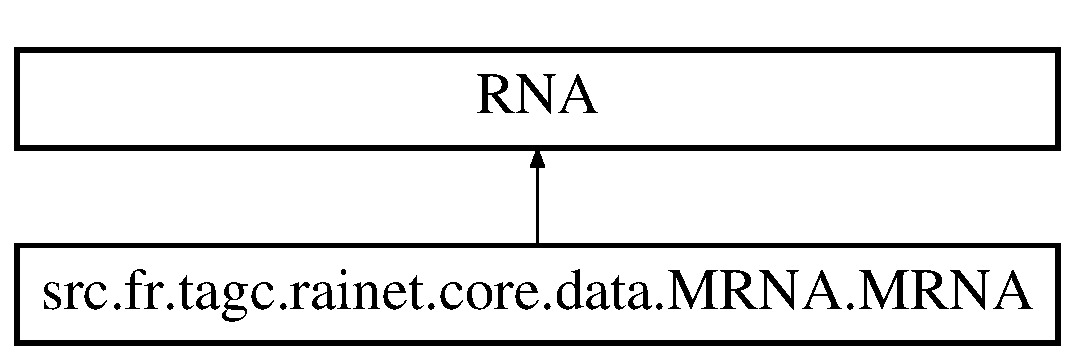
\includegraphics[height=2.000000cm]{classsrc_1_1fr_1_1tagc_1_1rainet_1_1core_1_1data_1_1MRNA_1_1MRNA}
\end{center}
\end{figure}
\subsection*{Public Member Functions}
\begin{DoxyCompactItemize}
\item 
\hypertarget{classsrc_1_1fr_1_1tagc_1_1rainet_1_1core_1_1data_1_1MRNA_1_1MRNA_a374fb3ea9bb548ab697e4e80aa55f93c}{def {\bfseries \-\_\-\-\_\-init\-\_\-\-\_\-}}\label{classsrc_1_1fr_1_1tagc_1_1rainet_1_1core_1_1data_1_1MRNA_1_1MRNA_a374fb3ea9bb548ab697e4e80aa55f93c}

\end{DoxyCompactItemize}
\subsection*{Public Attributes}
\begin{DoxyCompactItemize}
\item 
\hypertarget{classsrc_1_1fr_1_1tagc_1_1rainet_1_1core_1_1data_1_1MRNA_1_1MRNA_aba511061d3d2861e6d08b5d1d42387bf}{{\bfseries protein\-I\-D}}\label{classsrc_1_1fr_1_1tagc_1_1rainet_1_1core_1_1data_1_1MRNA_1_1MRNA_aba511061d3d2861e6d08b5d1d42387bf}

\end{DoxyCompactItemize}
\subsection*{Static Public Attributes}
\begin{DoxyCompactItemize}
\item 
\hypertarget{classsrc_1_1fr_1_1tagc_1_1rainet_1_1core_1_1data_1_1MRNA_1_1MRNA_a68d34a6659a265cc9a3f80134d075d59}{tuple {\bfseries transcript\-I\-D} = Column( String, Foreign\-Key('R\-N\-A.\-transcript\-I\-D'), primary\-\_\-key=True)}\label{classsrc_1_1fr_1_1tagc_1_1rainet_1_1core_1_1data_1_1MRNA_1_1MRNA_a68d34a6659a265cc9a3f80134d075d59}

\item 
\hypertarget{classsrc_1_1fr_1_1tagc_1_1rainet_1_1core_1_1data_1_1MRNA_1_1MRNA_a28db07076ce4e5ec9a4bf7d2d330cc72}{tuple {\bfseries protein\-I\-D} = Column( String, Foreign\-Key( 'Protein.\-uniprot\-A\-C'))}\label{classsrc_1_1fr_1_1tagc_1_1rainet_1_1core_1_1data_1_1MRNA_1_1MRNA_a28db07076ce4e5ec9a4bf7d2d330cc72}

\end{DoxyCompactItemize}


The documentation for this class was generated from the following file\-:\begin{DoxyCompactItemize}
\item 
src/fr/tagc/rainet/core/data/M\-R\-N\-A.\-py\end{DoxyCompactItemize}

\hypertarget{classsrc_1_1fr_1_1tagc_1_1rainet_1_1core_1_1data_1_1NetworkModule_1_1NetworkModule}{\section{src.\-fr.\-tagc.\-rainet.\-core.\-data.\-Network\-Module.\-Network\-Module Class Reference}
\label{classsrc_1_1fr_1_1tagc_1_1rainet_1_1core_1_1data_1_1NetworkModule_1_1NetworkModule}\index{src.\-fr.\-tagc.\-rainet.\-core.\-data.\-Network\-Module.\-Network\-Module@{src.\-fr.\-tagc.\-rainet.\-core.\-data.\-Network\-Module.\-Network\-Module}}
}


This class describes a Network Module (a group of interacting proteins) as produced by a network partition analysis like O\-C\-G.  


Inheritance diagram for src.\-fr.\-tagc.\-rainet.\-core.\-data.\-Network\-Module.\-Network\-Module\-:\begin{figure}[H]
\begin{center}
\leavevmode
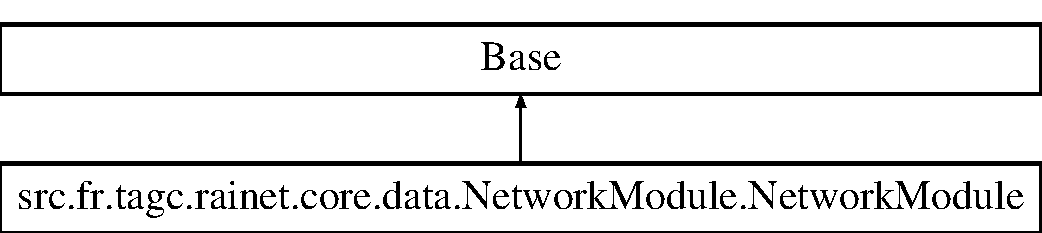
\includegraphics[height=2.000000cm]{classsrc_1_1fr_1_1tagc_1_1rainet_1_1core_1_1data_1_1NetworkModule_1_1NetworkModule}
\end{center}
\end{figure}
\subsection*{Public Member Functions}
\begin{DoxyCompactItemize}
\item 
\hypertarget{classsrc_1_1fr_1_1tagc_1_1rainet_1_1core_1_1data_1_1NetworkModule_1_1NetworkModule_aaba2991b15d8ccd23c7a927eba14eac8}{def \hyperlink{classsrc_1_1fr_1_1tagc_1_1rainet_1_1core_1_1data_1_1NetworkModule_1_1NetworkModule_aaba2991b15d8ccd23c7a927eba14eac8}{\-\_\-\-\_\-init\-\_\-\-\_\-}}\label{classsrc_1_1fr_1_1tagc_1_1rainet_1_1core_1_1data_1_1NetworkModule_1_1NetworkModule_aaba2991b15d8ccd23c7a927eba14eac8}

\begin{DoxyCompactList}\small\item\em The constructor. \end{DoxyCompactList}\item 
\hypertarget{classsrc_1_1fr_1_1tagc_1_1rainet_1_1core_1_1data_1_1NetworkModule_1_1NetworkModule_a4761e5200abaf04c59d4c8af761acb86}{def \hyperlink{classsrc_1_1fr_1_1tagc_1_1rainet_1_1core_1_1data_1_1NetworkModule_1_1NetworkModule_a4761e5200abaf04c59d4c8af761acb86}{add\-\_\-associated\-\_\-protein}}\label{classsrc_1_1fr_1_1tagc_1_1rainet_1_1core_1_1data_1_1NetworkModule_1_1NetworkModule_a4761e5200abaf04c59d4c8af761acb86}

\begin{DoxyCompactList}\small\item\em Add an associated protein to the list. \end{DoxyCompactList}\item 
\hypertarget{classsrc_1_1fr_1_1tagc_1_1rainet_1_1core_1_1data_1_1NetworkModule_1_1NetworkModule_a2b38ec7fc64cec9a13edb72955cfd34f}{def \hyperlink{classsrc_1_1fr_1_1tagc_1_1rainet_1_1core_1_1data_1_1NetworkModule_1_1NetworkModule_a2b38ec7fc64cec9a13edb72955cfd34f}{add\-\_\-associated\-\_\-annotation}}\label{classsrc_1_1fr_1_1tagc_1_1rainet_1_1core_1_1data_1_1NetworkModule_1_1NetworkModule_a2b38ec7fc64cec9a13edb72955cfd34f}

\begin{DoxyCompactList}\small\item\em Add an associated annotation to the list. \end{DoxyCompactList}\end{DoxyCompactItemize}
\subsection*{Public Attributes}
\begin{DoxyCompactItemize}
\item 
\hypertarget{classsrc_1_1fr_1_1tagc_1_1rainet_1_1core_1_1data_1_1NetworkModule_1_1NetworkModule_a0de546c5e35e1ddfc4a05c317de97b48}{{\bfseries module\-I\-D}}\label{classsrc_1_1fr_1_1tagc_1_1rainet_1_1core_1_1data_1_1NetworkModule_1_1NetworkModule_a0de546c5e35e1ddfc4a05c317de97b48}

\end{DoxyCompactItemize}
\subsection*{Static Public Attributes}
\begin{DoxyCompactItemize}
\item 
\hypertarget{classsrc_1_1fr_1_1tagc_1_1rainet_1_1core_1_1data_1_1NetworkModule_1_1NetworkModule_ab06d07b3543741afb05826e3ec611206}{tuple {\bfseries module\-I\-D} = Column( String, primary\-\_\-key = True )}\label{classsrc_1_1fr_1_1tagc_1_1rainet_1_1core_1_1data_1_1NetworkModule_1_1NetworkModule_ab06d07b3543741afb05826e3ec611206}

\item 
\hypertarget{classsrc_1_1fr_1_1tagc_1_1rainet_1_1core_1_1data_1_1NetworkModule_1_1NetworkModule_af105d7d1e7b91a3b779c2bb5ffa8feb6}{tuple {\bfseries partition\-Analysis\-\_\-id} = Column( String, Foreign\-Key('Partition\-Analysis.\-analysis\-Name'))}\label{classsrc_1_1fr_1_1tagc_1_1rainet_1_1core_1_1data_1_1NetworkModule_1_1NetworkModule_af105d7d1e7b91a3b779c2bb5ffa8feb6}

\item 
\hypertarget{classsrc_1_1fr_1_1tagc_1_1rainet_1_1core_1_1data_1_1NetworkModule_1_1NetworkModule_a6a0c59be82d0603a9b7106be205af7ec}{tuple {\bfseries associated\-Proteins} = relationship('Protein', secondary=Protein\-Network\-Module.\-\_\-\-\_\-table\-\_\-\-\_\-, backref=\char`\"{}network\-Modules\char`\"{})}\label{classsrc_1_1fr_1_1tagc_1_1rainet_1_1core_1_1data_1_1NetworkModule_1_1NetworkModule_a6a0c59be82d0603a9b7106be205af7ec}

\item 
\hypertarget{classsrc_1_1fr_1_1tagc_1_1rainet_1_1core_1_1data_1_1NetworkModule_1_1NetworkModule_a956f518c1f903e5625727fb0ac41ace8}{tuple {\bfseries associated\-Annotations} = relationship( 'Network\-Module\-Annotation', backref= \char`\"{}network\-Module\char`\"{})}\label{classsrc_1_1fr_1_1tagc_1_1rainet_1_1core_1_1data_1_1NetworkModule_1_1NetworkModule_a956f518c1f903e5625727fb0ac41ace8}

\end{DoxyCompactItemize}


\subsection{Detailed Description}
This class describes a Network Module (a group of interacting proteins) as produced by a network partition analysis like O\-C\-G. 

The documentation for this class was generated from the following file\-:\begin{DoxyCompactItemize}
\item 
src/fr/tagc/rainet/core/data/Network\-Module.\-py\end{DoxyCompactItemize}

\hypertarget{classsrc_1_1fr_1_1tagc_1_1rainet_1_1core_1_1data_1_1NetworkModuleAnnotation_1_1NetworkModuleAnnotation}{\section{src.\-fr.\-tagc.\-rainet.\-core.\-data.\-Network\-Module\-Annotation.\-Network\-Module\-Annotation Class Reference}
\label{classsrc_1_1fr_1_1tagc_1_1rainet_1_1core_1_1data_1_1NetworkModuleAnnotation_1_1NetworkModuleAnnotation}\index{src.\-fr.\-tagc.\-rainet.\-core.\-data.\-Network\-Module\-Annotation.\-Network\-Module\-Annotation@{src.\-fr.\-tagc.\-rainet.\-core.\-data.\-Network\-Module\-Annotation.\-Network\-Module\-Annotation}}
}


This class describes a Network Module (a group of interacting proteins) as produced by a network partition analysis like O\-C\-G.  


Inheritance diagram for src.\-fr.\-tagc.\-rainet.\-core.\-data.\-Network\-Module\-Annotation.\-Network\-Module\-Annotation\-:\begin{figure}[H]
\begin{center}
\leavevmode
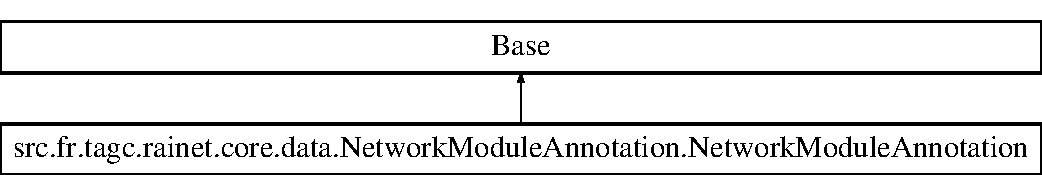
\includegraphics[height=2.000000cm]{classsrc_1_1fr_1_1tagc_1_1rainet_1_1core_1_1data_1_1NetworkModuleAnnotation_1_1NetworkModuleAnnotation}
\end{center}
\end{figure}
\subsection*{Public Member Functions}
\begin{DoxyCompactItemize}
\item 
\hypertarget{classsrc_1_1fr_1_1tagc_1_1rainet_1_1core_1_1data_1_1NetworkModuleAnnotation_1_1NetworkModuleAnnotation_aee2e9099e4e32b5aaac46841ab38a620}{def \hyperlink{classsrc_1_1fr_1_1tagc_1_1rainet_1_1core_1_1data_1_1NetworkModuleAnnotation_1_1NetworkModuleAnnotation_aee2e9099e4e32b5aaac46841ab38a620}{\-\_\-\-\_\-init\-\_\-\-\_\-}}\label{classsrc_1_1fr_1_1tagc_1_1rainet_1_1core_1_1data_1_1NetworkModuleAnnotation_1_1NetworkModuleAnnotation_aee2e9099e4e32b5aaac46841ab38a620}

\begin{DoxyCompactList}\small\item\em The constructor. \end{DoxyCompactList}\end{DoxyCompactItemize}
\subsection*{Public Attributes}
\begin{DoxyCompactItemize}
\item 
\hypertarget{classsrc_1_1fr_1_1tagc_1_1rainet_1_1core_1_1data_1_1NetworkModuleAnnotation_1_1NetworkModuleAnnotation_a8d150b3706e2cbbedfc284ab56ba2537}{{\bfseries annotation\-Name}}\label{classsrc_1_1fr_1_1tagc_1_1rainet_1_1core_1_1data_1_1NetworkModuleAnnotation_1_1NetworkModuleAnnotation_a8d150b3706e2cbbedfc284ab56ba2537}

\item 
\hypertarget{classsrc_1_1fr_1_1tagc_1_1rainet_1_1core_1_1data_1_1NetworkModuleAnnotation_1_1NetworkModuleAnnotation_aadc624c9f9757f8558a7309fc43110bf}{{\bfseries annotation\-I\-D}}\label{classsrc_1_1fr_1_1tagc_1_1rainet_1_1core_1_1data_1_1NetworkModuleAnnotation_1_1NetworkModuleAnnotation_aadc624c9f9757f8558a7309fc43110bf}

\end{DoxyCompactItemize}
\subsection*{Static Public Attributes}
\begin{DoxyCompactItemize}
\item 
\hypertarget{classsrc_1_1fr_1_1tagc_1_1rainet_1_1core_1_1data_1_1NetworkModuleAnnotation_1_1NetworkModuleAnnotation_a64f32f49c6e01cd418b1cf9da76156c6}{tuple {\bfseries network\-Module\-\_\-id} = Column( String, Foreign\-Key('Network\-Module.\-module\-I\-D') )}\label{classsrc_1_1fr_1_1tagc_1_1rainet_1_1core_1_1data_1_1NetworkModuleAnnotation_1_1NetworkModuleAnnotation_a64f32f49c6e01cd418b1cf9da76156c6}

\item 
\hypertarget{classsrc_1_1fr_1_1tagc_1_1rainet_1_1core_1_1data_1_1NetworkModuleAnnotation_1_1NetworkModuleAnnotation_a543791f68dbbfc29b55c96bd60835d4e}{tuple {\bfseries annotation\-I\-D} = Column( String )}\label{classsrc_1_1fr_1_1tagc_1_1rainet_1_1core_1_1data_1_1NetworkModuleAnnotation_1_1NetworkModuleAnnotation_a543791f68dbbfc29b55c96bd60835d4e}

\item 
\hypertarget{classsrc_1_1fr_1_1tagc_1_1rainet_1_1core_1_1data_1_1NetworkModuleAnnotation_1_1NetworkModuleAnnotation_a5112a9a1a65ac621f94db6baf2c4efbd}{tuple {\bfseries annotation\-Term} = Column( String )}\label{classsrc_1_1fr_1_1tagc_1_1rainet_1_1core_1_1data_1_1NetworkModuleAnnotation_1_1NetworkModuleAnnotation_a5112a9a1a65ac621f94db6baf2c4efbd}

\end{DoxyCompactItemize}


\subsection{Detailed Description}
This class describes a Network Module (a group of interacting proteins) as produced by a network partition analysis like O\-C\-G. 

The documentation for this class was generated from the following file\-:\begin{DoxyCompactItemize}
\item 
src/fr/tagc/rainet/core/data/Network\-Module\-Annotation.\-py\end{DoxyCompactItemize}

\hypertarget{classsrc_1_1fr_1_1tagc_1_1rainet_1_1core_1_1util_1_1parser_1_1NetworkModuleAnnotationParser_1_1NetworkModuleAnnotationParser}{\section{src.\-fr.\-tagc.\-rainet.\-core.\-util.\-parser.\-Network\-Module\-Annotation\-Parser.\-Network\-Module\-Annotation\-Parser Class Reference}
\label{classsrc_1_1fr_1_1tagc_1_1rainet_1_1core_1_1util_1_1parser_1_1NetworkModuleAnnotationParser_1_1NetworkModuleAnnotationParser}\index{src.\-fr.\-tagc.\-rainet.\-core.\-util.\-parser.\-Network\-Module\-Annotation\-Parser.\-Network\-Module\-Annotation\-Parser@{src.\-fr.\-tagc.\-rainet.\-core.\-util.\-parser.\-Network\-Module\-Annotation\-Parser.\-Network\-Module\-Annotation\-Parser}}
}


This class is a parser of a graph module (class) annotation file produced by the Brun team tools Each retrieved module get its annotations added The parser have to received as input\-: -\/file\-\_\-path \-: string -\/ The fpath to the file to parse -\/class\-\_\-tag \-: string -\/ The tag indicating the beginning of a class (module) definition -\/class\-\_\-regex \-: string -\/ The regex that provides the location of the class (module) I\-D as a group -\/protein\-\_\-tag \-: string -\/ The tag indicating the list of class (module) proteins -\/annotation\-\_\-tag \-: string -\/ The tag indicating the list of class (module) annotations -\/comment\-\_\-char \-: string -\/ The character used to declare comment lines -\/clean\-\_\-table \-: boolean -\/ The information indicating if the related db table must be cleaned before insertion or not.  


Inheritance diagram for src.\-fr.\-tagc.\-rainet.\-core.\-util.\-parser.\-Network\-Module\-Annotation\-Parser.\-Network\-Module\-Annotation\-Parser\-:\begin{figure}[H]
\begin{center}
\leavevmode
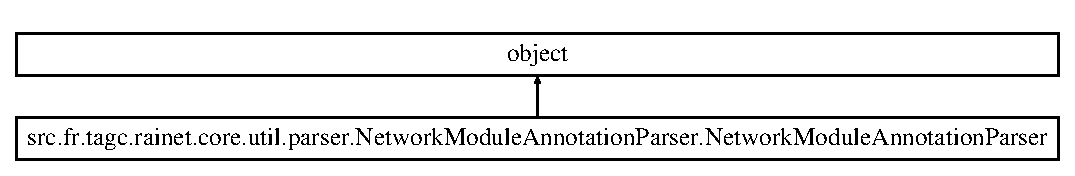
\includegraphics[height=1.911263cm]{classsrc_1_1fr_1_1tagc_1_1rainet_1_1core_1_1util_1_1parser_1_1NetworkModuleAnnotationParser_1_1NetworkModuleAnnotationParser}
\end{center}
\end{figure}
\subsection*{Static Public Member Functions}
\begin{DoxyCompactItemize}
\item 
\hypertarget{classsrc_1_1fr_1_1tagc_1_1rainet_1_1core_1_1util_1_1parser_1_1NetworkModuleAnnotationParser_1_1NetworkModuleAnnotationParser_a0f615babb23b0308ccbe7ee86ee1d3a0}{def {\bfseries parse\-\_\-file}}\label{classsrc_1_1fr_1_1tagc_1_1rainet_1_1core_1_1util_1_1parser_1_1NetworkModuleAnnotationParser_1_1NetworkModuleAnnotationParser_a0f615babb23b0308ccbe7ee86ee1d3a0}

\item 
\hypertarget{classsrc_1_1fr_1_1tagc_1_1rainet_1_1core_1_1util_1_1parser_1_1NetworkModuleAnnotationParser_1_1NetworkModuleAnnotationParser_aca6c2c2d14d6ca166152de814c3d70fc}{def {\bfseries process\-\_\-modules}}\label{classsrc_1_1fr_1_1tagc_1_1rainet_1_1core_1_1util_1_1parser_1_1NetworkModuleAnnotationParser_1_1NetworkModuleAnnotationParser_aca6c2c2d14d6ca166152de814c3d70fc}

\item 
def \hyperlink{classsrc_1_1fr_1_1tagc_1_1rainet_1_1core_1_1util_1_1parser_1_1NetworkModuleAnnotationParser_1_1NetworkModuleAnnotationParser_ae635f6f43b72b7649c779786dd32779b}{check\-\_\-proteins}
\begin{DoxyCompactList}\small\item\em Check if the list of proteins provided in the list correspond to the network module proteins listed in the D\-B. \end{DoxyCompactList}\item 
def \hyperlink{classsrc_1_1fr_1_1tagc_1_1rainet_1_1core_1_1util_1_1parser_1_1NetworkModuleAnnotationParser_1_1NetworkModuleAnnotationParser_a5239cf8f1385df4b488a50c6b468aff2}{associate\-\_\-annotations}
\begin{DoxyCompactList}\small\item\em Parse the provided line to find annotations. \end{DoxyCompactList}\end{DoxyCompactItemize}


\subsection{Detailed Description}
This class is a parser of a graph module (class) annotation file produced by the Brun team tools Each retrieved module get its annotations added The parser have to received as input\-: -\/file\-\_\-path \-: string -\/ The fpath to the file to parse -\/class\-\_\-tag \-: string -\/ The tag indicating the beginning of a class (module) definition -\/class\-\_\-regex \-: string -\/ The regex that provides the location of the class (module) I\-D as a group -\/protein\-\_\-tag \-: string -\/ The tag indicating the list of class (module) proteins -\/annotation\-\_\-tag \-: string -\/ The tag indicating the list of class (module) annotations -\/comment\-\_\-char \-: string -\/ The character used to declare comment lines -\/clean\-\_\-table \-: boolean -\/ The information indicating if the related db table must be cleaned before insertion or not. 

\subsection{Member Function Documentation}
\hypertarget{classsrc_1_1fr_1_1tagc_1_1rainet_1_1core_1_1util_1_1parser_1_1NetworkModuleAnnotationParser_1_1NetworkModuleAnnotationParser_a5239cf8f1385df4b488a50c6b468aff2}{\index{src\-::fr\-::tagc\-::rainet\-::core\-::util\-::parser\-::\-Network\-Module\-Annotation\-Parser\-::\-Network\-Module\-Annotation\-Parser@{src\-::fr\-::tagc\-::rainet\-::core\-::util\-::parser\-::\-Network\-Module\-Annotation\-Parser\-::\-Network\-Module\-Annotation\-Parser}!associate\-\_\-annotations@{associate\-\_\-annotations}}
\index{associate\-\_\-annotations@{associate\-\_\-annotations}!src::fr::tagc::rainet::core::util::parser::NetworkModuleAnnotationParser::NetworkModuleAnnotationParser@{src\-::fr\-::tagc\-::rainet\-::core\-::util\-::parser\-::\-Network\-Module\-Annotation\-Parser\-::\-Network\-Module\-Annotation\-Parser}}
\subsubsection[{associate\-\_\-annotations}]{\setlength{\rightskip}{0pt plus 5cm}def src.\-fr.\-tagc.\-rainet.\-core.\-util.\-parser.\-Network\-Module\-Annotation\-Parser.\-Network\-Module\-Annotation\-Parser.\-associate\-\_\-annotations (
\begin{DoxyParamCaption}
\item[{}]{network\-\_\-module, }
\item[{}]{line, }
\item[{}]{sql\-\_\-session}
\end{DoxyParamCaption}
)\hspace{0.3cm}{\ttfamily [static]}}}\label{classsrc_1_1fr_1_1tagc_1_1rainet_1_1core_1_1util_1_1parser_1_1NetworkModuleAnnotationParser_1_1NetworkModuleAnnotationParser_a5239cf8f1385df4b488a50c6b468aff2}


Parse the provided line to find annotations. 

Create corresponding Network\-Module\-Annotation objects and attach them to the provided network\-\_\-module


\begin{DoxyParams}{Parameters}
{\em network\-\_\-module} & \-: Network\-Module -\/ The annotated network module \\
\hline
{\em line} & \-: string -\/ the line of the file containing the list of annotations \\
\hline
{\em sql\-\_\-session} & the current S\-Q\-L\-Alchemy session\\
\hline
\end{DoxyParams}
\begin{DoxyReturn}{Returns}
None  Rainet\-Exception if an error occurred during parsing 
\end{DoxyReturn}
\hypertarget{classsrc_1_1fr_1_1tagc_1_1rainet_1_1core_1_1util_1_1parser_1_1NetworkModuleAnnotationParser_1_1NetworkModuleAnnotationParser_ae635f6f43b72b7649c779786dd32779b}{\index{src\-::fr\-::tagc\-::rainet\-::core\-::util\-::parser\-::\-Network\-Module\-Annotation\-Parser\-::\-Network\-Module\-Annotation\-Parser@{src\-::fr\-::tagc\-::rainet\-::core\-::util\-::parser\-::\-Network\-Module\-Annotation\-Parser\-::\-Network\-Module\-Annotation\-Parser}!check\-\_\-proteins@{check\-\_\-proteins}}
\index{check\-\_\-proteins@{check\-\_\-proteins}!src::fr::tagc::rainet::core::util::parser::NetworkModuleAnnotationParser::NetworkModuleAnnotationParser@{src\-::fr\-::tagc\-::rainet\-::core\-::util\-::parser\-::\-Network\-Module\-Annotation\-Parser\-::\-Network\-Module\-Annotation\-Parser}}
\subsubsection[{check\-\_\-proteins}]{\setlength{\rightskip}{0pt plus 5cm}def src.\-fr.\-tagc.\-rainet.\-core.\-util.\-parser.\-Network\-Module\-Annotation\-Parser.\-Network\-Module\-Annotation\-Parser.\-check\-\_\-proteins (
\begin{DoxyParamCaption}
\item[{}]{network\-\_\-module, }
\item[{}]{line, }
\item[{}]{sql\-\_\-session}
\end{DoxyParamCaption}
)\hspace{0.3cm}{\ttfamily [static]}}}\label{classsrc_1_1fr_1_1tagc_1_1rainet_1_1core_1_1util_1_1parser_1_1NetworkModuleAnnotationParser_1_1NetworkModuleAnnotationParser_ae635f6f43b72b7649c779786dd32779b}


Check if the list of proteins provided in the list correspond to the network module proteins listed in the D\-B. 


\begin{DoxyParams}{Parameters}
{\em network\-\_\-module} & \-: Network\-Module -\/ The network module the proteins should be part of \\
\hline
{\em line} & \-: string -\/ the line of the file containing the list of proteins \\
\hline
{\em sql\-\_\-session} & the current S\-Q\-L\-Alchemy session\\
\hline
\end{DoxyParams}
\begin{DoxyReturn}{Returns}
None  Rainet\-Exception if an error occurred during parsing 
\end{DoxyReturn}


The documentation for this class was generated from the following file\-:\begin{DoxyCompactItemize}
\item 
src/fr/tagc/rainet/core/util/parser/Network\-Module\-Annotation\-Parser.\-py\end{DoxyCompactItemize}

\hypertarget{classsrc_1_1fr_1_1tagc_1_1rainet_1_1core_1_1execution_1_1analysis_1_1EnrichmentAnalysis_1_1Netwocd24f37753b2377449d55719611022ad}{\section{src.\-fr.\-tagc.\-rainet.\-core.\-execution.\-analysis.\-Enrichment\-Analysis.\-Network\-Module\-G\-O\-Terms.\-Network\-Module\-G\-O\-Terms Class Reference}
\label{classsrc_1_1fr_1_1tagc_1_1rainet_1_1core_1_1execution_1_1analysis_1_1EnrichmentAnalysis_1_1Netwocd24f37753b2377449d55719611022ad}\index{src.\-fr.\-tagc.\-rainet.\-core.\-execution.\-analysis.\-Enrichment\-Analysis.\-Network\-Module\-G\-O\-Terms.\-Network\-Module\-G\-O\-Terms@{src.\-fr.\-tagc.\-rainet.\-core.\-execution.\-analysis.\-Enrichment\-Analysis.\-Network\-Module\-G\-O\-Terms.\-Network\-Module\-G\-O\-Terms}}
}
Inheritance diagram for src.\-fr.\-tagc.\-rainet.\-core.\-execution.\-analysis.\-Enrichment\-Analysis.\-Network\-Module\-G\-O\-Terms.\-Network\-Module\-G\-O\-Terms\-:\begin{figure}[H]
\begin{center}
\leavevmode
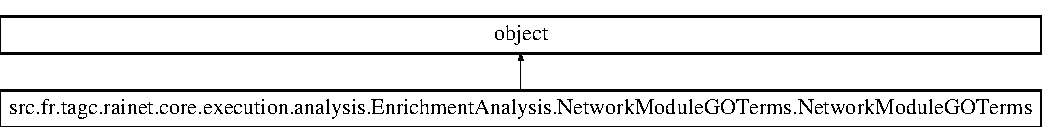
\includegraphics[height=1.702128cm]{classsrc_1_1fr_1_1tagc_1_1rainet_1_1core_1_1execution_1_1analysis_1_1EnrichmentAnalysis_1_1Netwocd24f37753b2377449d55719611022ad}
\end{center}
\end{figure}
\subsection*{Public Member Functions}
\begin{DoxyCompactItemize}
\item 
\hypertarget{classsrc_1_1fr_1_1tagc_1_1rainet_1_1core_1_1execution_1_1analysis_1_1EnrichmentAnalysis_1_1Netwocd24f37753b2377449d55719611022ad_aaa6d11be9d27f31c5ad22798f0b3c3c4}{def {\bfseries \-\_\-\-\_\-init\-\_\-\-\_\-}}\label{classsrc_1_1fr_1_1tagc_1_1rainet_1_1core_1_1execution_1_1analysis_1_1EnrichmentAnalysis_1_1Netwocd24f37753b2377449d55719611022ad_aaa6d11be9d27f31c5ad22798f0b3c3c4}

\item 
\hypertarget{classsrc_1_1fr_1_1tagc_1_1rainet_1_1core_1_1execution_1_1analysis_1_1EnrichmentAnalysis_1_1Netwocd24f37753b2377449d55719611022ad_ad698c6e018b2cd9580ab19f316f9b4bc}{def {\bfseries read\-\_\-rainet\-\_\-db}}\label{classsrc_1_1fr_1_1tagc_1_1rainet_1_1core_1_1execution_1_1analysis_1_1EnrichmentAnalysis_1_1Netwocd24f37753b2377449d55719611022ad_ad698c6e018b2cd9580ab19f316f9b4bc}

\item 
\hypertarget{classsrc_1_1fr_1_1tagc_1_1rainet_1_1core_1_1execution_1_1analysis_1_1EnrichmentAnalysis_1_1Netwocd24f37753b2377449d55719611022ad_aa7de88037fafd1c1eca1b3e10f5b7bed}{def {\bfseries read\-\_\-enrichment\-\_\-file}}\label{classsrc_1_1fr_1_1tagc_1_1rainet_1_1core_1_1execution_1_1analysis_1_1EnrichmentAnalysis_1_1Netwocd24f37753b2377449d55719611022ad_aa7de88037fafd1c1eca1b3e10f5b7bed}

\item 
\hypertarget{classsrc_1_1fr_1_1tagc_1_1rainet_1_1core_1_1execution_1_1analysis_1_1EnrichmentAnalysis_1_1Netwocd24f37753b2377449d55719611022ad_abc193f41717940429053bfc8d8f05706}{def {\bfseries run}}\label{classsrc_1_1fr_1_1tagc_1_1rainet_1_1core_1_1execution_1_1analysis_1_1EnrichmentAnalysis_1_1Netwocd24f37753b2377449d55719611022ad_abc193f41717940429053bfc8d8f05706}

\end{DoxyCompactItemize}
\subsection*{Public Attributes}
\begin{DoxyCompactItemize}
\item 
\hypertarget{classsrc_1_1fr_1_1tagc_1_1rainet_1_1core_1_1execution_1_1analysis_1_1EnrichmentAnalysis_1_1Netwocd24f37753b2377449d55719611022ad_a198714ef7b14e2d6372eb8093f07e774}{{\bfseries enrichment\-File}}\label{classsrc_1_1fr_1_1tagc_1_1rainet_1_1core_1_1execution_1_1analysis_1_1EnrichmentAnalysis_1_1Netwocd24f37753b2377449d55719611022ad_a198714ef7b14e2d6372eb8093f07e774}

\item 
\hypertarget{classsrc_1_1fr_1_1tagc_1_1rainet_1_1core_1_1execution_1_1analysis_1_1EnrichmentAnalysis_1_1Netwocd24f37753b2377449d55719611022ad_a765f9f4dad7152d10703b417c59072cc}{{\bfseries rainet\-D\-B}}\label{classsrc_1_1fr_1_1tagc_1_1rainet_1_1core_1_1execution_1_1analysis_1_1EnrichmentAnalysis_1_1Netwocd24f37753b2377449d55719611022ad_a765f9f4dad7152d10703b417c59072cc}

\item 
\hypertarget{classsrc_1_1fr_1_1tagc_1_1rainet_1_1core_1_1execution_1_1analysis_1_1EnrichmentAnalysis_1_1Netwocd24f37753b2377449d55719611022ad_a9fbf39aa40ddee00177701a92fce76ad}{{\bfseries output\-Folder}}\label{classsrc_1_1fr_1_1tagc_1_1rainet_1_1core_1_1execution_1_1analysis_1_1EnrichmentAnalysis_1_1Netwocd24f37753b2377449d55719611022ad_a9fbf39aa40ddee00177701a92fce76ad}

\item 
\hypertarget{classsrc_1_1fr_1_1tagc_1_1rainet_1_1core_1_1execution_1_1analysis_1_1EnrichmentAnalysis_1_1Netwocd24f37753b2377449d55719611022ad_abd969e3c90a0d9d1304d82394bd753d9}{{\bfseries sql\-\_\-session}}\label{classsrc_1_1fr_1_1tagc_1_1rainet_1_1core_1_1execution_1_1analysis_1_1EnrichmentAnalysis_1_1Netwocd24f37753b2377449d55719611022ad_abd969e3c90a0d9d1304d82394bd753d9}

\item 
\hypertarget{classsrc_1_1fr_1_1tagc_1_1rainet_1_1core_1_1execution_1_1analysis_1_1EnrichmentAnalysis_1_1Netwocd24f37753b2377449d55719611022ad_aabf48db6e38c87c869ab68f20655f9e6}{{\bfseries module\-G\-O\-Terms}}\label{classsrc_1_1fr_1_1tagc_1_1rainet_1_1core_1_1execution_1_1analysis_1_1EnrichmentAnalysis_1_1Netwocd24f37753b2377449d55719611022ad_aabf48db6e38c87c869ab68f20655f9e6}

\item 
\hypertarget{classsrc_1_1fr_1_1tagc_1_1rainet_1_1core_1_1execution_1_1analysis_1_1EnrichmentAnalysis_1_1Netwocd24f37753b2377449d55719611022ad_a6131178ad62562ebbca8319235c6de40}{{\bfseries go\-Term\-Frequency}}\label{classsrc_1_1fr_1_1tagc_1_1rainet_1_1core_1_1execution_1_1analysis_1_1EnrichmentAnalysis_1_1Netwocd24f37753b2377449d55719611022ad_a6131178ad62562ebbca8319235c6de40}

\item 
\hypertarget{classsrc_1_1fr_1_1tagc_1_1rainet_1_1core_1_1execution_1_1analysis_1_1EnrichmentAnalysis_1_1Netwocd24f37753b2377449d55719611022ad_ac96a935c2a4c9d1a7b11eca75beac3e3}{{\bfseries term\-Descriptions}}\label{classsrc_1_1fr_1_1tagc_1_1rainet_1_1core_1_1execution_1_1analysis_1_1EnrichmentAnalysis_1_1Netwocd24f37753b2377449d55719611022ad_ac96a935c2a4c9d1a7b11eca75beac3e3}

\end{DoxyCompactItemize}


The documentation for this class was generated from the following file\-:\begin{DoxyCompactItemize}
\item 
src/fr/tagc/rainet/core/execution/analysis/\-Enrichment\-Analysis/Network\-Module\-G\-O\-Terms.\-py\end{DoxyCompactItemize}

\hypertarget{classsrc_1_1fr_1_1tagc_1_1rainet_1_1core_1_1util_1_1parser_1_1NetworkModuleParser_1_1NetworkModuleParser}{\section{src.\-fr.\-tagc.\-rainet.\-core.\-util.\-parser.\-Network\-Module\-Parser.\-Network\-Module\-Parser Class Reference}
\label{classsrc_1_1fr_1_1tagc_1_1rainet_1_1core_1_1util_1_1parser_1_1NetworkModuleParser_1_1NetworkModuleParser}\index{src.\-fr.\-tagc.\-rainet.\-core.\-util.\-parser.\-Network\-Module\-Parser.\-Network\-Module\-Parser@{src.\-fr.\-tagc.\-rainet.\-core.\-util.\-parser.\-Network\-Module\-Parser.\-Network\-Module\-Parser}}
}


This class is a parser of a graph module (class) file produced by the Brun team tools Each retrieved module produces a Network\-Module and geta ssociated to the Protein that are part of it The parser have to received as input\-:  


Inheritance diagram for src.\-fr.\-tagc.\-rainet.\-core.\-util.\-parser.\-Network\-Module\-Parser.\-Network\-Module\-Parser\-:\begin{figure}[H]
\begin{center}
\leavevmode
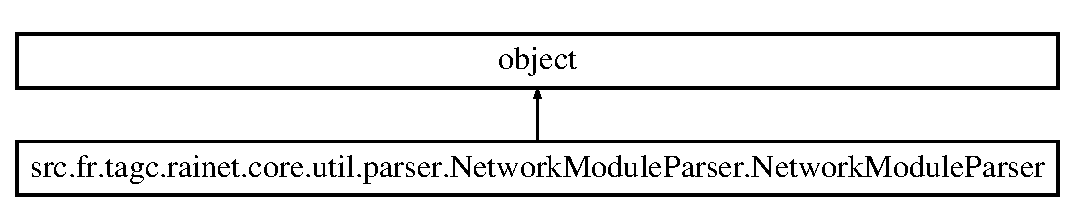
\includegraphics[height=2.000000cm]{classsrc_1_1fr_1_1tagc_1_1rainet_1_1core_1_1util_1_1parser_1_1NetworkModuleParser_1_1NetworkModuleParser}
\end{center}
\end{figure}
\subsection*{Static Public Member Functions}
\begin{DoxyCompactItemize}
\item 
\hypertarget{classsrc_1_1fr_1_1tagc_1_1rainet_1_1core_1_1util_1_1parser_1_1NetworkModuleParser_1_1NetworkModuleParser_a5621046e5c53b4a62832a5b9d9882ae8}{def {\bfseries parse\-\_\-file}}\label{classsrc_1_1fr_1_1tagc_1_1rainet_1_1core_1_1util_1_1parser_1_1NetworkModuleParser_1_1NetworkModuleParser_a5621046e5c53b4a62832a5b9d9882ae8}

\item 
\hypertarget{classsrc_1_1fr_1_1tagc_1_1rainet_1_1core_1_1util_1_1parser_1_1NetworkModuleParser_1_1NetworkModuleParser_a1fa9241a137a38fe50ed095e6a6ddcf7}{def {\bfseries process\-\_\-modules}}\label{classsrc_1_1fr_1_1tagc_1_1rainet_1_1core_1_1util_1_1parser_1_1NetworkModuleParser_1_1NetworkModuleParser_a1fa9241a137a38fe50ed095e6a6ddcf7}

\item 
def \hyperlink{classsrc_1_1fr_1_1tagc_1_1rainet_1_1core_1_1util_1_1parser_1_1NetworkModuleParser_1_1NetworkModuleParser_a3e0f2f9aa4e9b800e02676eb720765e2}{associate\-\_\-proteins}
\begin{DoxyCompactList}\small\item\em Parse the provided line to find protein names. \end{DoxyCompactList}\end{DoxyCompactItemize}


\subsection{Detailed Description}
This class is a parser of a graph module (class) file produced by the Brun team tools Each retrieved module produces a Network\-Module and geta ssociated to the Protein that are part of it The parser have to received as input\-: 


\begin{DoxyItemize}
\item file\-\_\-path \-: string -\/ The fpath to the file to parse
\item class\-\_\-tag \-: string -\/ The tag indicating the beginning of a class (module) definition
\item comment\-\_\-char \-: string -\/ The character used to declare comment lines
\item clean\-\_\-table \-: boolean -\/ The information indicating if the related db table must be cleaned before insertion or not 
\end{DoxyItemize}

\subsection{Member Function Documentation}
\hypertarget{classsrc_1_1fr_1_1tagc_1_1rainet_1_1core_1_1util_1_1parser_1_1NetworkModuleParser_1_1NetworkModuleParser_a3e0f2f9aa4e9b800e02676eb720765e2}{\index{src\-::fr\-::tagc\-::rainet\-::core\-::util\-::parser\-::\-Network\-Module\-Parser\-::\-Network\-Module\-Parser@{src\-::fr\-::tagc\-::rainet\-::core\-::util\-::parser\-::\-Network\-Module\-Parser\-::\-Network\-Module\-Parser}!associate\-\_\-proteins@{associate\-\_\-proteins}}
\index{associate\-\_\-proteins@{associate\-\_\-proteins}!src::fr::tagc::rainet::core::util::parser::NetworkModuleParser::NetworkModuleParser@{src\-::fr\-::tagc\-::rainet\-::core\-::util\-::parser\-::\-Network\-Module\-Parser\-::\-Network\-Module\-Parser}}
\subsubsection[{associate\-\_\-proteins}]{\setlength{\rightskip}{0pt plus 5cm}def src.\-fr.\-tagc.\-rainet.\-core.\-util.\-parser.\-Network\-Module\-Parser.\-Network\-Module\-Parser.\-associate\-\_\-proteins (
\begin{DoxyParamCaption}
\item[{}]{module, }
\item[{}]{line}
\end{DoxyParamCaption}
)\hspace{0.3cm}{\ttfamily [static]}}}\label{classsrc_1_1fr_1_1tagc_1_1rainet_1_1core_1_1util_1_1parser_1_1NetworkModuleParser_1_1NetworkModuleParser_a3e0f2f9aa4e9b800e02676eb720765e2}


Parse the provided line to find protein names. 

Create corresponding association between the proteins and the module


\begin{DoxyParams}{Parameters}
{\em module} & \-: Network\-Module -\/ The network module the proteins must be associated to \\
\hline
{\em line} & \-: string -\/ the line of the file containing the list of protein names\\
\hline
\end{DoxyParams}
\begin{DoxyReturn}{Returns}
None  Rainet\-Exception if an error occurred during parsing 
\end{DoxyReturn}


The documentation for this class was generated from the following file\-:\begin{DoxyCompactItemize}
\item 
src/fr/tagc/rainet/core/util/parser/Network\-Module\-Parser.\-py\end{DoxyCompactItemize}

\hypertarget{classsrc_1_1fr_1_1tagc_1_1rainet_1_1core_1_1execution_1_1analysis_1_1NetworkScoreAnalysis_1_1Netb8ffb1b7ba97f5d739cfb51f5ce47153}{\section{src.\-fr.\-tagc.\-rainet.\-core.\-execution.\-analysis.\-Network\-Score\-Analysis.\-Network\-Score\-Analysis.\-Network\-Score\-Analysis Class Reference}
\label{classsrc_1_1fr_1_1tagc_1_1rainet_1_1core_1_1execution_1_1analysis_1_1NetworkScoreAnalysis_1_1Netb8ffb1b7ba97f5d739cfb51f5ce47153}\index{src.\-fr.\-tagc.\-rainet.\-core.\-execution.\-analysis.\-Network\-Score\-Analysis.\-Network\-Score\-Analysis.\-Network\-Score\-Analysis@{src.\-fr.\-tagc.\-rainet.\-core.\-execution.\-analysis.\-Network\-Score\-Analysis.\-Network\-Score\-Analysis.\-Network\-Score\-Analysis}}
}
Inheritance diagram for src.\-fr.\-tagc.\-rainet.\-core.\-execution.\-analysis.\-Network\-Score\-Analysis.\-Network\-Score\-Analysis.\-Network\-Score\-Analysis\-:\begin{figure}[H]
\begin{center}
\leavevmode
\includegraphics[height=1.725732cm]{classsrc_1_1fr_1_1tagc_1_1rainet_1_1core_1_1execution_1_1analysis_1_1NetworkScoreAnalysis_1_1Netb8ffb1b7ba97f5d739cfb51f5ce47153}
\end{center}
\end{figure}
\subsection*{Public Member Functions}
\begin{DoxyCompactItemize}
\item 
\hypertarget{classsrc_1_1fr_1_1tagc_1_1rainet_1_1core_1_1execution_1_1analysis_1_1NetworkScoreAnalysis_1_1Netb8ffb1b7ba97f5d739cfb51f5ce47153_af75c3279fd46a02f78e7047f6a7a4816}{def {\bfseries \-\_\-\-\_\-init\-\_\-\-\_\-}}\label{classsrc_1_1fr_1_1tagc_1_1rainet_1_1core_1_1execution_1_1analysis_1_1NetworkScoreAnalysis_1_1Netb8ffb1b7ba97f5d739cfb51f5ce47153_af75c3279fd46a02f78e7047f6a7a4816}

\item 
\hypertarget{classsrc_1_1fr_1_1tagc_1_1rainet_1_1core_1_1execution_1_1analysis_1_1NetworkScoreAnalysis_1_1Netb8ffb1b7ba97f5d739cfb51f5ce47153_aea1a900bef5c839f6f082c46bed3acc1}{def {\bfseries read\-\_\-network\-\_\-file}}\label{classsrc_1_1fr_1_1tagc_1_1rainet_1_1core_1_1execution_1_1analysis_1_1NetworkScoreAnalysis_1_1Netb8ffb1b7ba97f5d739cfb51f5ce47153_aea1a900bef5c839f6f082c46bed3acc1}

\item 
\hypertarget{classsrc_1_1fr_1_1tagc_1_1rainet_1_1core_1_1execution_1_1analysis_1_1NetworkScoreAnalysis_1_1Netb8ffb1b7ba97f5d739cfb51f5ce47153_a03648d32643fcd6d712e1c34c9636212}{def {\bfseries calculate\-\_\-protein\-\_\-degree}}\label{classsrc_1_1fr_1_1tagc_1_1rainet_1_1core_1_1execution_1_1analysis_1_1NetworkScoreAnalysis_1_1Netb8ffb1b7ba97f5d739cfb51f5ce47153_a03648d32643fcd6d712e1c34c9636212}

\item 
\hypertarget{classsrc_1_1fr_1_1tagc_1_1rainet_1_1core_1_1execution_1_1analysis_1_1NetworkScoreAnalysis_1_1Netb8ffb1b7ba97f5d739cfb51f5ce47153_a65b5d8c647eca2acecc5fc714894caa2}{def {\bfseries read\-\_\-catrapid\-\_\-file}}\label{classsrc_1_1fr_1_1tagc_1_1rainet_1_1core_1_1execution_1_1analysis_1_1NetworkScoreAnalysis_1_1Netb8ffb1b7ba97f5d739cfb51f5ce47153_a65b5d8c647eca2acecc5fc714894caa2}

\item 
\hypertarget{classsrc_1_1fr_1_1tagc_1_1rainet_1_1core_1_1execution_1_1analysis_1_1NetworkScoreAnalysis_1_1Netb8ffb1b7ba97f5d739cfb51f5ce47153_af4eacb81439f8e0509fedb3978b99830}{def {\bfseries pick\-\_\-top\-\_\-proteins}}\label{classsrc_1_1fr_1_1tagc_1_1rainet_1_1core_1_1execution_1_1analysis_1_1NetworkScoreAnalysis_1_1Netb8ffb1b7ba97f5d739cfb51f5ce47153_af4eacb81439f8e0509fedb3978b99830}

\item 
\hypertarget{classsrc_1_1fr_1_1tagc_1_1rainet_1_1core_1_1execution_1_1analysis_1_1NetworkScoreAnalysis_1_1Netb8ffb1b7ba97f5d739cfb51f5ce47153_a75922fae959caff93b94c1c162b0f205}{def {\bfseries calculate\-\_\-metrics}}\label{classsrc_1_1fr_1_1tagc_1_1rainet_1_1core_1_1execution_1_1analysis_1_1NetworkScoreAnalysis_1_1Netb8ffb1b7ba97f5d739cfb51f5ce47153_a75922fae959caff93b94c1c162b0f205}

\item 
\hypertarget{classsrc_1_1fr_1_1tagc_1_1rainet_1_1core_1_1execution_1_1analysis_1_1NetworkScoreAnalysis_1_1Netb8ffb1b7ba97f5d739cfb51f5ce47153_aa38cd1f70057cfcccc9a70b33cd78051}{def {\bfseries run}}\label{classsrc_1_1fr_1_1tagc_1_1rainet_1_1core_1_1execution_1_1analysis_1_1NetworkScoreAnalysis_1_1Netb8ffb1b7ba97f5d739cfb51f5ce47153_aa38cd1f70057cfcccc9a70b33cd78051}

\end{DoxyCompactItemize}
\subsection*{Public Attributes}
\begin{DoxyCompactItemize}
\item 
\hypertarget{classsrc_1_1fr_1_1tagc_1_1rainet_1_1core_1_1execution_1_1analysis_1_1NetworkScoreAnalysis_1_1Netb8ffb1b7ba97f5d739cfb51f5ce47153_a61be67c0c8021f3d04c3f0dc95f8ff1c}{{\bfseries network\-File}}\label{classsrc_1_1fr_1_1tagc_1_1rainet_1_1core_1_1execution_1_1analysis_1_1NetworkScoreAnalysis_1_1Netb8ffb1b7ba97f5d739cfb51f5ce47153_a61be67c0c8021f3d04c3f0dc95f8ff1c}

\item 
\hypertarget{classsrc_1_1fr_1_1tagc_1_1rainet_1_1core_1_1execution_1_1analysis_1_1NetworkScoreAnalysis_1_1Netb8ffb1b7ba97f5d739cfb51f5ce47153_a636351d3af7157bae2b392b85aff9d40}{{\bfseries catrapid\-File}}\label{classsrc_1_1fr_1_1tagc_1_1rainet_1_1core_1_1execution_1_1analysis_1_1NetworkScoreAnalysis_1_1Netb8ffb1b7ba97f5d739cfb51f5ce47153_a636351d3af7157bae2b392b85aff9d40}

\item 
\hypertarget{classsrc_1_1fr_1_1tagc_1_1rainet_1_1core_1_1execution_1_1analysis_1_1NetworkScoreAnalysis_1_1Netb8ffb1b7ba97f5d739cfb51f5ce47153_a5b17ebba9149a99f03fea22eeb2ec612}{{\bfseries top\-Partners}}\label{classsrc_1_1fr_1_1tagc_1_1rainet_1_1core_1_1execution_1_1analysis_1_1NetworkScoreAnalysis_1_1Netb8ffb1b7ba97f5d739cfb51f5ce47153_a5b17ebba9149a99f03fea22eeb2ec612}

\item 
\hypertarget{classsrc_1_1fr_1_1tagc_1_1rainet_1_1core_1_1execution_1_1analysis_1_1NetworkScoreAnalysis_1_1Netb8ffb1b7ba97f5d739cfb51f5ce47153_aca491976f53097655ab169be7f739973}{{\bfseries output\-Folder}}\label{classsrc_1_1fr_1_1tagc_1_1rainet_1_1core_1_1execution_1_1analysis_1_1NetworkScoreAnalysis_1_1Netb8ffb1b7ba97f5d739cfb51f5ce47153_aca491976f53097655ab169be7f739973}

\item 
\hypertarget{classsrc_1_1fr_1_1tagc_1_1rainet_1_1core_1_1execution_1_1analysis_1_1NetworkScoreAnalysis_1_1Netb8ffb1b7ba97f5d739cfb51f5ce47153_a76a16cf589506cf73acd4438007f22fc}{{\bfseries number\-Randomizations}}\label{classsrc_1_1fr_1_1tagc_1_1rainet_1_1core_1_1execution_1_1analysis_1_1NetworkScoreAnalysis_1_1Netb8ffb1b7ba97f5d739cfb51f5ce47153_a76a16cf589506cf73acd4438007f22fc}

\item 
\hypertarget{classsrc_1_1fr_1_1tagc_1_1rainet_1_1core_1_1execution_1_1analysis_1_1NetworkScoreAnalysis_1_1Netb8ffb1b7ba97f5d739cfb51f5ce47153_ad5caa35c261f773c315234a08294fb9c}{{\bfseries calculated\-Shortest\-Paths}}\label{classsrc_1_1fr_1_1tagc_1_1rainet_1_1core_1_1execution_1_1analysis_1_1NetworkScoreAnalysis_1_1Netb8ffb1b7ba97f5d739cfb51f5ce47153_ad5caa35c261f773c315234a08294fb9c}

\item 
\hypertarget{classsrc_1_1fr_1_1tagc_1_1rainet_1_1core_1_1execution_1_1analysis_1_1NetworkScoreAnalysis_1_1Netb8ffb1b7ba97f5d739cfb51f5ce47153_a6bb2e2a7eafcfe03d74aebc74b1f27f9}{{\bfseries graph}}\label{classsrc_1_1fr_1_1tagc_1_1rainet_1_1core_1_1execution_1_1analysis_1_1NetworkScoreAnalysis_1_1Netb8ffb1b7ba97f5d739cfb51f5ce47153_a6bb2e2a7eafcfe03d74aebc74b1f27f9}

\item 
\hypertarget{classsrc_1_1fr_1_1tagc_1_1rainet_1_1core_1_1execution_1_1analysis_1_1NetworkScoreAnalysis_1_1Netb8ffb1b7ba97f5d739cfb51f5ce47153_a2bd45acfd15db9319f2aee6fc17aad9d}{{\bfseries protein\-Graph\-I\-D\-Dict}}\label{classsrc_1_1fr_1_1tagc_1_1rainet_1_1core_1_1execution_1_1analysis_1_1NetworkScoreAnalysis_1_1Netb8ffb1b7ba97f5d739cfb51f5ce47153_a2bd45acfd15db9319f2aee6fc17aad9d}

\item 
\hypertarget{classsrc_1_1fr_1_1tagc_1_1rainet_1_1core_1_1execution_1_1analysis_1_1NetworkScoreAnalysis_1_1Netb8ffb1b7ba97f5d739cfb51f5ce47153_a87fdce9d482885e50338f379b7990088}{{\bfseries dict\-Names}}\label{classsrc_1_1fr_1_1tagc_1_1rainet_1_1core_1_1execution_1_1analysis_1_1NetworkScoreAnalysis_1_1Netb8ffb1b7ba97f5d739cfb51f5ce47153_a87fdce9d482885e50338f379b7990088}

\item 
\hypertarget{classsrc_1_1fr_1_1tagc_1_1rainet_1_1core_1_1execution_1_1analysis_1_1NetworkScoreAnalysis_1_1Netb8ffb1b7ba97f5d739cfb51f5ce47153_a43f68169269bc897a0fcdecc1e169002}{\hyperlink{classsrc_1_1fr_1_1tagc_1_1rainet_1_1core_1_1execution_1_1analysis_1_1NetworkScoreAnalysis_1_1Netb8ffb1b7ba97f5d739cfb51f5ce47153_a43f68169269bc897a0fcdecc1e169002}{degree\-Dict}}\label{classsrc_1_1fr_1_1tagc_1_1rainet_1_1core_1_1execution_1_1analysis_1_1NetworkScoreAnalysis_1_1Netb8ffb1b7ba97f5d739cfb51f5ce47153_a43f68169269bc897a0fcdecc1e169002}

\begin{DoxyCompactList}\small\item\em list of degrees available, so that closest degree to the degree of interest can be probed sorted\-Degrees = sorted( proteins\-Per\-Degree\-Dict.\-keys()) \end{DoxyCompactList}\item 
\hypertarget{classsrc_1_1fr_1_1tagc_1_1rainet_1_1core_1_1execution_1_1analysis_1_1NetworkScoreAnalysis_1_1Netb8ffb1b7ba97f5d739cfb51f5ce47153_a6cff73af45334d208933ce5412bf42d6}{{\bfseries proteins\-Per\-Degree\-Dict}}\label{classsrc_1_1fr_1_1tagc_1_1rainet_1_1core_1_1execution_1_1analysis_1_1NetworkScoreAnalysis_1_1Netb8ffb1b7ba97f5d739cfb51f5ce47153_a6cff73af45334d208933ce5412bf42d6}

\item 
\hypertarget{classsrc_1_1fr_1_1tagc_1_1rainet_1_1core_1_1execution_1_1analysis_1_1NetworkScoreAnalysis_1_1Netb8ffb1b7ba97f5d739cfb51f5ce47153_a1bff6b67d1460ec94d5b0505b87cd5bc}{\hyperlink{classsrc_1_1fr_1_1tagc_1_1rainet_1_1core_1_1execution_1_1analysis_1_1NetworkScoreAnalysis_1_1Netb8ffb1b7ba97f5d739cfb51f5ce47153_a1bff6b67d1460ec94d5b0505b87cd5bc}{rna\-Targets}}\label{classsrc_1_1fr_1_1tagc_1_1rainet_1_1core_1_1execution_1_1analysis_1_1NetworkScoreAnalysis_1_1Netb8ffb1b7ba97f5d739cfb51f5ce47153_a1bff6b67d1460ec94d5b0505b87cd5bc}

\begin{DoxyCompactList}\small\item\em R\-N\-A side. \end{DoxyCompactList}\item 
\hypertarget{classsrc_1_1fr_1_1tagc_1_1rainet_1_1core_1_1execution_1_1analysis_1_1NetworkScoreAnalysis_1_1Netb8ffb1b7ba97f5d739cfb51f5ce47153_ad0e16c559af066a93a370ab1c4177669}{{\bfseries all\-Prot\-Set}}\label{classsrc_1_1fr_1_1tagc_1_1rainet_1_1core_1_1execution_1_1analysis_1_1NetworkScoreAnalysis_1_1Netb8ffb1b7ba97f5d739cfb51f5ce47153_ad0e16c559af066a93a370ab1c4177669}

\item 
\hypertarget{classsrc_1_1fr_1_1tagc_1_1rainet_1_1core_1_1execution_1_1analysis_1_1NetworkScoreAnalysis_1_1Netb8ffb1b7ba97f5d739cfb51f5ce47153_a24be30ca7519eec1f694f6e57693536e}{{\bfseries all\-R\-N\-A\-Set}}\label{classsrc_1_1fr_1_1tagc_1_1rainet_1_1core_1_1execution_1_1analysis_1_1NetworkScoreAnalysis_1_1Netb8ffb1b7ba97f5d739cfb51f5ce47153_a24be30ca7519eec1f694f6e57693536e}

\item 
\hypertarget{classsrc_1_1fr_1_1tagc_1_1rainet_1_1core_1_1execution_1_1analysis_1_1NetworkScoreAnalysis_1_1Netb8ffb1b7ba97f5d739cfb51f5ce47153_a5059eb56ada25aef8364e3e484409570}{{\bfseries rna\-Tops}}\label{classsrc_1_1fr_1_1tagc_1_1rainet_1_1core_1_1execution_1_1analysis_1_1NetworkScoreAnalysis_1_1Netb8ffb1b7ba97f5d739cfb51f5ce47153_a5059eb56ada25aef8364e3e484409570}

\end{DoxyCompactItemize}
\subsection*{Static Public Attributes}
\begin{DoxyCompactItemize}
\item 
dictionary {\bfseries D\-I\-S\-T\-A\-N\-C\-E\-\_\-\-S\-C\-O\-R\-E}
\item 
\hypertarget{classsrc_1_1fr_1_1tagc_1_1rainet_1_1core_1_1execution_1_1analysis_1_1NetworkScoreAnalysis_1_1Netb8ffb1b7ba97f5d739cfb51f5ce47153_a4b05a89b10881db1984f91e06f3aef30}{float {\bfseries D\-I\-S\-T\-A\-N\-C\-E\-\_\-\-A\-B\-O\-V\-E\-\_\-\-L\-I\-M\-I\-T\-\_\-\-S\-C\-O\-R\-E} = -\/0.\-1}\label{classsrc_1_1fr_1_1tagc_1_1rainet_1_1core_1_1execution_1_1analysis_1_1NetworkScoreAnalysis_1_1Netb8ffb1b7ba97f5d739cfb51f5ce47153_a4b05a89b10881db1984f91e06f3aef30}

\item 
\hypertarget{classsrc_1_1fr_1_1tagc_1_1rainet_1_1core_1_1execution_1_1analysis_1_1NetworkScoreAnalysis_1_1Netb8ffb1b7ba97f5d739cfb51f5ce47153_af2265e84739b1cee9330b098efc2a636}{int {\bfseries M\-A\-X\-I\-M\-U\-M\-\_\-\-N\-U\-M\-B\-E\-R\-\_\-\-V\-I\-A\-B\-L\-E\-\_\-\-I\-N\-T\-E\-R\-A\-C\-T\-I\-O\-N\-S} = 100000000}\label{classsrc_1_1fr_1_1tagc_1_1rainet_1_1core_1_1execution_1_1analysis_1_1NetworkScoreAnalysis_1_1Netb8ffb1b7ba97f5d739cfb51f5ce47153_af2265e84739b1cee9330b098efc2a636}

\item 
\hypertarget{classsrc_1_1fr_1_1tagc_1_1rainet_1_1core_1_1execution_1_1analysis_1_1NetworkScoreAnalysis_1_1Netb8ffb1b7ba97f5d739cfb51f5ce47153_ab353f8bde016f7379bd6ebb74e675b9e}{string {\bfseries P\-A\-R\-A\-M\-E\-T\-E\-R\-S\-\_\-\-L\-O\-G} = \char`\"{}parameters.\-log\char`\"{}}\label{classsrc_1_1fr_1_1tagc_1_1rainet_1_1core_1_1execution_1_1analysis_1_1NetworkScoreAnalysis_1_1Netb8ffb1b7ba97f5d739cfb51f5ce47153_ab353f8bde016f7379bd6ebb74e675b9e}

\item 
\hypertarget{classsrc_1_1fr_1_1tagc_1_1rainet_1_1core_1_1execution_1_1analysis_1_1NetworkScoreAnalysis_1_1Netb8ffb1b7ba97f5d739cfb51f5ce47153_ad9974ddef7280dcd9d0900560a31600d}{string {\bfseries R\-E\-P\-O\-R\-T\-\_\-\-M\-E\-T\-R\-I\-C\-S\-\_\-\-O\-U\-T\-P\-U\-T} = \char`\"{}metrics\-\_\-per\-\_\-rna.\-tsv\char`\"{}}\label{classsrc_1_1fr_1_1tagc_1_1rainet_1_1core_1_1execution_1_1analysis_1_1NetworkScoreAnalysis_1_1Netb8ffb1b7ba97f5d739cfb51f5ce47153_ad9974ddef7280dcd9d0900560a31600d}

\end{DoxyCompactItemize}


\subsection{Member Data Documentation}
\hypertarget{classsrc_1_1fr_1_1tagc_1_1rainet_1_1core_1_1execution_1_1analysis_1_1NetworkScoreAnalysis_1_1Netb8ffb1b7ba97f5d739cfb51f5ce47153_a13d4d3bff64e807f9a8427f0d437ddd2}{\index{src\-::fr\-::tagc\-::rainet\-::core\-::execution\-::analysis\-::\-Network\-Score\-Analysis\-::\-Network\-Score\-Analysis\-::\-Network\-Score\-Analysis@{src\-::fr\-::tagc\-::rainet\-::core\-::execution\-::analysis\-::\-Network\-Score\-Analysis\-::\-Network\-Score\-Analysis\-::\-Network\-Score\-Analysis}!D\-I\-S\-T\-A\-N\-C\-E\-\_\-\-S\-C\-O\-R\-E@{D\-I\-S\-T\-A\-N\-C\-E\-\_\-\-S\-C\-O\-R\-E}}
\index{D\-I\-S\-T\-A\-N\-C\-E\-\_\-\-S\-C\-O\-R\-E@{D\-I\-S\-T\-A\-N\-C\-E\-\_\-\-S\-C\-O\-R\-E}!src::fr::tagc::rainet::core::execution::analysis::NetworkScoreAnalysis::NetworkScoreAnalysis::NetworkScoreAnalysis@{src\-::fr\-::tagc\-::rainet\-::core\-::execution\-::analysis\-::\-Network\-Score\-Analysis\-::\-Network\-Score\-Analysis\-::\-Network\-Score\-Analysis}}
\subsubsection[{D\-I\-S\-T\-A\-N\-C\-E\-\_\-\-S\-C\-O\-R\-E}]{\setlength{\rightskip}{0pt plus 5cm}dictionary src.\-fr.\-tagc.\-rainet.\-core.\-execution.\-analysis.\-Network\-Score\-Analysis.\-Network\-Score\-Analysis.\-Network\-Score\-Analysis.\-D\-I\-S\-T\-A\-N\-C\-E\-\_\-\-S\-C\-O\-R\-E\hspace{0.3cm}{\ttfamily [static]}}}\label{classsrc_1_1fr_1_1tagc_1_1rainet_1_1core_1_1execution_1_1analysis_1_1NetworkScoreAnalysis_1_1Netb8ffb1b7ba97f5d739cfb51f5ce47153_a13d4d3bff64e807f9a8427f0d437ddd2}
{\bfseries Initial value\-:}
\begin{DoxyCode}
1 = \{
2                       1 : 1,
3                       2 : 0.5,
4                       3 : 0.25 \}
\end{DoxyCode}


The documentation for this class was generated from the following file\-:\begin{DoxyCompactItemize}
\item 
src/fr/tagc/rainet/core/execution/analysis/\-Network\-Score\-Analysis/Network\-Score\-Analysis.\-py\end{DoxyCompactItemize}

\hypertarget{classanalysis_1_1NetworkScoreAnalysisUnittest_1_1NetworkScoreAnalysisUnittest}{\section{analysis.\-Network\-Score\-Analysis\-Unittest.\-Network\-Score\-Analysis\-Unittest Class Reference}
\label{classanalysis_1_1NetworkScoreAnalysisUnittest_1_1NetworkScoreAnalysisUnittest}\index{analysis.\-Network\-Score\-Analysis\-Unittest.\-Network\-Score\-Analysis\-Unittest@{analysis.\-Network\-Score\-Analysis\-Unittest.\-Network\-Score\-Analysis\-Unittest}}
}
Inheritance diagram for analysis.\-Network\-Score\-Analysis\-Unittest.\-Network\-Score\-Analysis\-Unittest\-:\begin{figure}[H]
\begin{center}
\leavevmode
\includegraphics[height=2.000000cm]{classanalysis_1_1NetworkScoreAnalysisUnittest_1_1NetworkScoreAnalysisUnittest}
\end{center}
\end{figure}
\subsection*{Public Member Functions}
\begin{DoxyCompactItemize}
\item 
\hypertarget{classanalysis_1_1NetworkScoreAnalysisUnittest_1_1NetworkScoreAnalysisUnittest_ad4f81210a9065bb123f1d7d70637011f}{def {\bfseries set\-Up}}\label{classanalysis_1_1NetworkScoreAnalysisUnittest_1_1NetworkScoreAnalysisUnittest_ad4f81210a9065bb123f1d7d70637011f}

\item 
\hypertarget{classanalysis_1_1NetworkScoreAnalysisUnittest_1_1NetworkScoreAnalysisUnittest_aaab7fbe23c99902c865af37d34bd96ef}{def {\bfseries test\-\_\-read\-\_\-network\-\_\-file}}\label{classanalysis_1_1NetworkScoreAnalysisUnittest_1_1NetworkScoreAnalysisUnittest_aaab7fbe23c99902c865af37d34bd96ef}

\item 
\hypertarget{classanalysis_1_1NetworkScoreAnalysisUnittest_1_1NetworkScoreAnalysisUnittest_a90068eae66d2451db91565dcc46770e3}{def {\bfseries test\-\_\-calculate\-\_\-protein\-\_\-degree}}\label{classanalysis_1_1NetworkScoreAnalysisUnittest_1_1NetworkScoreAnalysisUnittest_a90068eae66d2451db91565dcc46770e3}

\item 
\hypertarget{classanalysis_1_1NetworkScoreAnalysisUnittest_1_1NetworkScoreAnalysisUnittest_aacc13a44c0841a0f7e34b72db9f107ae}{def {\bfseries test\-\_\-read\-\_\-catrapid\-\_\-file}}\label{classanalysis_1_1NetworkScoreAnalysisUnittest_1_1NetworkScoreAnalysisUnittest_aacc13a44c0841a0f7e34b72db9f107ae}

\item 
\hypertarget{classanalysis_1_1NetworkScoreAnalysisUnittest_1_1NetworkScoreAnalysisUnittest_aa1f7503b01eb3b195941d1566ebfb9b6}{def {\bfseries test\-\_\-pick\-\_\-top\-\_\-proteins}}\label{classanalysis_1_1NetworkScoreAnalysisUnittest_1_1NetworkScoreAnalysisUnittest_aa1f7503b01eb3b195941d1566ebfb9b6}

\item 
\hypertarget{classanalysis_1_1NetworkScoreAnalysisUnittest_1_1NetworkScoreAnalysisUnittest_a8d865bcc5a3bc7789e09ac06cda51969}{def {\bfseries test\-\_\-calculate\-\_\-metric\-\_\-for\-\_\-rna}}\label{classanalysis_1_1NetworkScoreAnalysisUnittest_1_1NetworkScoreAnalysisUnittest_a8d865bcc5a3bc7789e09ac06cda51969}

\item 
\hypertarget{classanalysis_1_1NetworkScoreAnalysisUnittest_1_1NetworkScoreAnalysisUnittest_a4f2d057cc92115132759023cc3bb573a}{def {\bfseries test\-\_\-get\-\_\-sample\-\_\-protein\-\_\-degree}}\label{classanalysis_1_1NetworkScoreAnalysisUnittest_1_1NetworkScoreAnalysisUnittest_a4f2d057cc92115132759023cc3bb573a}

\item 
\hypertarget{classanalysis_1_1NetworkScoreAnalysisUnittest_1_1NetworkScoreAnalysisUnittest_aa6f291544a77dc684a5f33043775af69}{def {\bfseries test\-\_\-get\-\_\-new\-\_\-degree}}\label{classanalysis_1_1NetworkScoreAnalysisUnittest_1_1NetworkScoreAnalysisUnittest_aa6f291544a77dc684a5f33043775af69}

\item 
\hypertarget{classanalysis_1_1NetworkScoreAnalysisUnittest_1_1NetworkScoreAnalysisUnittest_a75575ab5836afae23867bda5d359c13d}{def {\bfseries test\-\_\-calculate\-\_\-metrics}}\label{classanalysis_1_1NetworkScoreAnalysisUnittest_1_1NetworkScoreAnalysisUnittest_a75575ab5836afae23867bda5d359c13d}

\item 
\hypertarget{classanalysis_1_1NetworkScoreAnalysisUnittest_1_1NetworkScoreAnalysisUnittest_ab3e14bed9f754f5a2cd3bcfe7e1c0197}{def {\bfseries test\-\_\-multi\-\_\-top\-Partners}}\label{classanalysis_1_1NetworkScoreAnalysisUnittest_1_1NetworkScoreAnalysisUnittest_ab3e14bed9f754f5a2cd3bcfe7e1c0197}

\item 
\hypertarget{classanalysis_1_1NetworkScoreAnalysisUnittest_1_1NetworkScoreAnalysisUnittest_ac391f04a8f33c5919ab2fe0c2ce1b74a}{def {\bfseries test\-\_\-run}}\label{classanalysis_1_1NetworkScoreAnalysisUnittest_1_1NetworkScoreAnalysisUnittest_ac391f04a8f33c5919ab2fe0c2ce1b74a}

\end{DoxyCompactItemize}
\subsection*{Public Attributes}
\begin{DoxyCompactItemize}
\item 
\hypertarget{classanalysis_1_1NetworkScoreAnalysisUnittest_1_1NetworkScoreAnalysisUnittest_a8111ea541c81dcae8bb42ea72c919295}{{\bfseries network\-File}}\label{classanalysis_1_1NetworkScoreAnalysisUnittest_1_1NetworkScoreAnalysisUnittest_a8111ea541c81dcae8bb42ea72c919295}

\item 
\hypertarget{classanalysis_1_1NetworkScoreAnalysisUnittest_1_1NetworkScoreAnalysisUnittest_ab2e6c213b613cc016afec08c17fbea0d}{{\bfseries catrapid\-File}}\label{classanalysis_1_1NetworkScoreAnalysisUnittest_1_1NetworkScoreAnalysisUnittest_ab2e6c213b613cc016afec08c17fbea0d}

\item 
\hypertarget{classanalysis_1_1NetworkScoreAnalysisUnittest_1_1NetworkScoreAnalysisUnittest_ab8d569d584a81fc0c4d48d9e46ec7b44}{{\bfseries top\-Partners}}\label{classanalysis_1_1NetworkScoreAnalysisUnittest_1_1NetworkScoreAnalysisUnittest_ab8d569d584a81fc0c4d48d9e46ec7b44}

\item 
\hypertarget{classanalysis_1_1NetworkScoreAnalysisUnittest_1_1NetworkScoreAnalysisUnittest_a4bb6bd8d96cb484b455205e6e0f76505}{{\bfseries top\-Partners\-Single}}\label{classanalysis_1_1NetworkScoreAnalysisUnittest_1_1NetworkScoreAnalysisUnittest_a4bb6bd8d96cb484b455205e6e0f76505}

\item 
\hypertarget{classanalysis_1_1NetworkScoreAnalysisUnittest_1_1NetworkScoreAnalysisUnittest_ad476bce89cad474995ec14a5f5aadfb6}{{\bfseries output\-Folder}}\label{classanalysis_1_1NetworkScoreAnalysisUnittest_1_1NetworkScoreAnalysisUnittest_ad476bce89cad474995ec14a5f5aadfb6}

\item 
\hypertarget{classanalysis_1_1NetworkScoreAnalysisUnittest_1_1NetworkScoreAnalysisUnittest_a36086c4c86183a73880d9757653775af}{{\bfseries number\-Randomizations}}\label{classanalysis_1_1NetworkScoreAnalysisUnittest_1_1NetworkScoreAnalysisUnittest_a36086c4c86183a73880d9757653775af}

\item 
\hypertarget{classanalysis_1_1NetworkScoreAnalysisUnittest_1_1NetworkScoreAnalysisUnittest_acba47618f5fb8b38a4f7e499d8b0fffa}{{\bfseries run}}\label{classanalysis_1_1NetworkScoreAnalysisUnittest_1_1NetworkScoreAnalysisUnittest_acba47618f5fb8b38a4f7e499d8b0fffa}

\end{DoxyCompactItemize}


The documentation for this class was generated from the following file\-:\begin{DoxyCompactItemize}
\item 
test/fr/tagc/rainet/core/execution/analysis/Network\-Score\-Analysis\-Unittest.\-py\end{DoxyCompactItemize}

\hypertarget{classsrc_1_1fr_1_1tagc_1_1rainet_1_1core_1_1util_1_1exception_1_1NotRequiredInstantiationExceptif1c629be8ad6f3196537937ab51f20ef}{\section{src.\-fr.\-tagc.\-rainet.\-core.\-util.\-exception.\-Not\-Required\-Instantiation\-Exception.\-Not\-Required\-Instantiation\-Exception Class Reference}
\label{classsrc_1_1fr_1_1tagc_1_1rainet_1_1core_1_1util_1_1exception_1_1NotRequiredInstantiationExceptif1c629be8ad6f3196537937ab51f20ef}\index{src.\-fr.\-tagc.\-rainet.\-core.\-util.\-exception.\-Not\-Required\-Instantiation\-Exception.\-Not\-Required\-Instantiation\-Exception@{src.\-fr.\-tagc.\-rainet.\-core.\-util.\-exception.\-Not\-Required\-Instantiation\-Exception.\-Not\-Required\-Instantiation\-Exception}}
}


This Exception is used when automatic instantiation is used through Factory and the class instantiation is not required since a similar object already exist (in D\-B for instance)  


Inheritance diagram for src.\-fr.\-tagc.\-rainet.\-core.\-util.\-exception.\-Not\-Required\-Instantiation\-Exception.\-Not\-Required\-Instantiation\-Exception\-:\begin{figure}[H]
\begin{center}
\leavevmode
\includegraphics[height=1.833061cm]{classsrc_1_1fr_1_1tagc_1_1rainet_1_1core_1_1util_1_1exception_1_1NotRequiredInstantiationExceptif1c629be8ad6f3196537937ab51f20ef}
\end{center}
\end{figure}
\subsection*{Public Member Functions}
\begin{DoxyCompactItemize}
\item 
\hypertarget{classsrc_1_1fr_1_1tagc_1_1rainet_1_1core_1_1util_1_1exception_1_1NotRequiredInstantiationExceptif1c629be8ad6f3196537937ab51f20ef_a84ba16b50af74c8f9cf46b1e8ff1fbc4}{def \hyperlink{classsrc_1_1fr_1_1tagc_1_1rainet_1_1core_1_1util_1_1exception_1_1NotRequiredInstantiationExceptif1c629be8ad6f3196537937ab51f20ef_a84ba16b50af74c8f9cf46b1e8ff1fbc4}{to\-\_\-string}}\label{classsrc_1_1fr_1_1tagc_1_1rainet_1_1core_1_1util_1_1exception_1_1NotRequiredInstantiationExceptif1c629be8ad6f3196537937ab51f20ef_a84ba16b50af74c8f9cf46b1e8ff1fbc4}

\begin{DoxyCompactList}\small\item\em Display the exception message and stack trace. \end{DoxyCompactList}\end{DoxyCompactItemize}


\subsection{Detailed Description}
This Exception is used when automatic instantiation is used through Factory and the class instantiation is not required since a similar object already exist (in D\-B for instance) 

The documentation for this class was generated from the following file\-:\begin{DoxyCompactItemize}
\item 
src/fr/tagc/rainet/core/util/exception/Not\-Required\-Instantiation\-Exception.\-py\end{DoxyCompactItemize}

\hypertarget{classNPInterPredictionValidation_1_1NPInterPredictionValidation}{\section{N\-P\-Inter\-Prediction\-Validation.\-N\-P\-Inter\-Prediction\-Validation Class Reference}
\label{classNPInterPredictionValidation_1_1NPInterPredictionValidation}\index{N\-P\-Inter\-Prediction\-Validation.\-N\-P\-Inter\-Prediction\-Validation@{N\-P\-Inter\-Prediction\-Validation.\-N\-P\-Inter\-Prediction\-Validation}}
}
Inheritance diagram for N\-P\-Inter\-Prediction\-Validation.\-N\-P\-Inter\-Prediction\-Validation\-:\begin{figure}[H]
\begin{center}
\leavevmode
\includegraphics[height=2.000000cm]{classNPInterPredictionValidation_1_1NPInterPredictionValidation}
\end{center}
\end{figure}
\subsection*{Public Member Functions}
\begin{DoxyCompactItemize}
\item 
\hypertarget{classNPInterPredictionValidation_1_1NPInterPredictionValidation_abdc4f5f41ebe3afc4e54bfe529a5f1df}{def {\bfseries \-\_\-\-\_\-init\-\_\-\-\_\-}}\label{classNPInterPredictionValidation_1_1NPInterPredictionValidation_abdc4f5f41ebe3afc4e54bfe529a5f1df}

\item 
\hypertarget{classNPInterPredictionValidation_1_1NPInterPredictionValidation_aa9a47d7585667373db10448b20f5aa56}{def {\bfseries proteins\-\_\-in\-\_\-rainet}}\label{classNPInterPredictionValidation_1_1NPInterPredictionValidation_aa9a47d7585667373db10448b20f5aa56}

\item 
\hypertarget{classNPInterPredictionValidation_1_1NPInterPredictionValidation_af37f25bf0c2ef1a6e733130e0e251b10}{def {\bfseries rna\-\_\-cross\-\_\-references}}\label{classNPInterPredictionValidation_1_1NPInterPredictionValidation_af37f25bf0c2ef1a6e733130e0e251b10}

\item 
\hypertarget{classNPInterPredictionValidation_1_1NPInterPredictionValidation_a32bd433cea86f0f186d8f0fa1b9c3798}{def {\bfseries read\-\_\-noncode\-\_\-conversion\-\_\-file}}\label{classNPInterPredictionValidation_1_1NPInterPredictionValidation_a32bd433cea86f0f186d8f0fa1b9c3798}

\item 
\hypertarget{classNPInterPredictionValidation_1_1NPInterPredictionValidation_a3505fdcdd05ad46b48237ab1505fb7d8}{def {\bfseries read\-\_\-\-N\-P\-Inter\-\_\-file}}\label{classNPInterPredictionValidation_1_1NPInterPredictionValidation_a3505fdcdd05ad46b48237ab1505fb7d8}

\item 
\hypertarget{classNPInterPredictionValidation_1_1NPInterPredictionValidation_a188641706e5e25962af1d6b00f22fbd3}{def {\bfseries read\-\_\-catrapid\-\_\-file}}\label{classNPInterPredictionValidation_1_1NPInterPredictionValidation_a188641706e5e25962af1d6b00f22fbd3}

\item 
\hypertarget{classNPInterPredictionValidation_1_1NPInterPredictionValidation_a5af0c0f0ffdb3a971ec0cdc65ec22778}{def {\bfseries read\-\_\-catrapid\-\_\-file\-\_\-new}}\label{classNPInterPredictionValidation_1_1NPInterPredictionValidation_a5af0c0f0ffdb3a971ec0cdc65ec22778}

\item 
\hypertarget{classNPInterPredictionValidation_1_1NPInterPredictionValidation_ae6d44876b9272cf01679c4433c17170d}{def {\bfseries read\-\_\-expression\-\_\-file}}\label{classNPInterPredictionValidation_1_1NPInterPredictionValidation_ae6d44876b9272cf01679c4433c17170d}

\end{DoxyCompactItemize}
\subsection*{Public Attributes}
\begin{DoxyCompactItemize}
\item 
\hypertarget{classNPInterPredictionValidation_1_1NPInterPredictionValidation_ac6e798155bfc489cf70957dd1e5796b8}{{\bfseries catrapid\-File}}\label{classNPInterPredictionValidation_1_1NPInterPredictionValidation_ac6e798155bfc489cf70957dd1e5796b8}

\item 
\hypertarget{classNPInterPredictionValidation_1_1NPInterPredictionValidation_aada3d7c02ed3328907ad22dcdb94b602}{{\bfseries npinter\-File}}\label{classNPInterPredictionValidation_1_1NPInterPredictionValidation_aada3d7c02ed3328907ad22dcdb94b602}

\item 
\hypertarget{classNPInterPredictionValidation_1_1NPInterPredictionValidation_a1e3eab2206d449835833ed86b63e22af}{{\bfseries noncode\-Tx2noncode\-Gene}}\label{classNPInterPredictionValidation_1_1NPInterPredictionValidation_a1e3eab2206d449835833ed86b63e22af}

\item 
\hypertarget{classNPInterPredictionValidation_1_1NPInterPredictionValidation_acab3cee7745f9c763325a0d7460496e1}{{\bfseries noncode2\-Ensembl}}\label{classNPInterPredictionValidation_1_1NPInterPredictionValidation_acab3cee7745f9c763325a0d7460496e1}

\item 
\hypertarget{classNPInterPredictionValidation_1_1NPInterPredictionValidation_aec06d81b65f801e532a7d6cb3e945320}{{\bfseries rainet\-D\-B}}\label{classNPInterPredictionValidation_1_1NPInterPredictionValidation_aec06d81b65f801e532a7d6cb3e945320}

\item 
\hypertarget{classNPInterPredictionValidation_1_1NPInterPredictionValidation_a761d84622155d69a05a2e1700c8e29fd}{{\bfseries output\-Folder}}\label{classNPInterPredictionValidation_1_1NPInterPredictionValidation_a761d84622155d69a05a2e1700c8e29fd}

\item 
\hypertarget{classNPInterPredictionValidation_1_1NPInterPredictionValidation_aee635dd2092f9c40c2cc1a05ae7ef709}{{\bfseries sql\-\_\-session}}\label{classNPInterPredictionValidation_1_1NPInterPredictionValidation_aee635dd2092f9c40c2cc1a05ae7ef709}

\item 
\hyperlink{classNPInterPredictionValidation_1_1NPInterPredictionValidation_aacd479a71f1a21704b6f7ff636a20885}{conversion\-Dict}
\begin{DoxyCompactList}\small\item\em 1) Read N\-O\-N\-C\-O\-D\-E transcript to N\-O\-N\-C\-O\-D\-E Gene I\-D e.\-g. \end{DoxyCompactList}\item 
\hypertarget{classNPInterPredictionValidation_1_1NPInterPredictionValidation_a2243689b917c2f82402a4c122d885c6b}{{\bfseries npinter\-Pairs}}\label{classNPInterPredictionValidation_1_1NPInterPredictionValidation_a2243689b917c2f82402a4c122d885c6b}

\end{DoxyCompactItemize}
\subsection*{Static Public Attributes}
\begin{DoxyCompactItemize}
\item 
\hypertarget{classNPInterPredictionValidation_1_1NPInterPredictionValidation_a82c33fcd8060dca24186301456fed0b4}{string {\bfseries S\-P\-E\-C\-I\-E\-S} = \char`\"{}Homo sapiens\char`\"{}}\label{classNPInterPredictionValidation_1_1NPInterPredictionValidation_a82c33fcd8060dca24186301456fed0b4}

\item 
\hypertarget{classNPInterPredictionValidation_1_1NPInterPredictionValidation_a1c1d89a3c24de55afb59c256002cf837}{string {\bfseries T\-A\-G} = \char`\"{}nc\-R\-N\-A-\/protein binding\char`\"{}}\label{classNPInterPredictionValidation_1_1NPInterPredictionValidation_a1c1d89a3c24de55afb59c256002cf837}

\item 
\hypertarget{classNPInterPredictionValidation_1_1NPInterPredictionValidation_a303956a866c498dede129a9023d9ee2b}{string {\bfseries I\-N\-T\-E\-R\-A\-C\-T\-I\-O\-N\-\_\-\-L\-E\-V\-E\-L} = \char`\"{}R\-N\-A-\/Protein\char`\"{}}\label{classNPInterPredictionValidation_1_1NPInterPredictionValidation_a303956a866c498dede129a9023d9ee2b}

\item 
\hypertarget{classNPInterPredictionValidation_1_1NPInterPredictionValidation_a652f7fc9d8d84a08b76b83850cde11e1}{string {\bfseries M\-O\-L\-E\-C\-U\-L\-E\-A\-D\-A\-T\-A\-B\-A\-S\-E} = \char`\"{}N\-O\-N\-C\-O\-D\-E\char`\"{}}\label{classNPInterPredictionValidation_1_1NPInterPredictionValidation_a652f7fc9d8d84a08b76b83850cde11e1}

\item 
\hypertarget{classNPInterPredictionValidation_1_1NPInterPredictionValidation_adefdbbad85aed10014220645774c33f3}{string {\bfseries D\-I\-S\-T\-R\-I\-B\-U\-T\-I\-O\-N\-\_\-\-S\-C\-R\-I\-P\-T} = \char`\"{}/home/diogo/workspace/tagc-\/rainet-\/R\-N\-A/src/fr/tagc/rainet/core/execution/processing/known\-Scaffold\-Examples/N\-P\-Inter\-\_\-stats.\-R\char`\"{}}\label{classNPInterPredictionValidation_1_1NPInterPredictionValidation_adefdbbad85aed10014220645774c33f3}

\end{DoxyCompactItemize}


\subsection{Member Data Documentation}
\hypertarget{classNPInterPredictionValidation_1_1NPInterPredictionValidation_aacd479a71f1a21704b6f7ff636a20885}{\index{N\-P\-Inter\-Prediction\-Validation\-::\-N\-P\-Inter\-Prediction\-Validation@{N\-P\-Inter\-Prediction\-Validation\-::\-N\-P\-Inter\-Prediction\-Validation}!conversion\-Dict@{conversion\-Dict}}
\index{conversion\-Dict@{conversion\-Dict}!NPInterPredictionValidation::NPInterPredictionValidation@{N\-P\-Inter\-Prediction\-Validation\-::\-N\-P\-Inter\-Prediction\-Validation}}
\subsubsection[{conversion\-Dict}]{\setlength{\rightskip}{0pt plus 5cm}N\-P\-Inter\-Prediction\-Validation.\-N\-P\-Inter\-Prediction\-Validation.\-conversion\-Dict}}\label{classNPInterPredictionValidation_1_1NPInterPredictionValidation_aacd479a71f1a21704b6f7ff636a20885}


1) Read N\-O\-N\-C\-O\-D\-E transcript to N\-O\-N\-C\-O\-D\-E Gene I\-D e.\-g. 

\subsection*{N\-O\-N\-H\-S\-A\-T000019.\-2 N\-O\-N\-H\-S\-A\-G000008.\-2 }

2) Read N\-O\-N\-C\-O\-D\-E transcript I\-D to Ensembl transcript I\-D \subsection*{e.\-g. N\-O\-N\-H\-S\-A\-T000012.\-1 ensembl E\-N\-S\-T00000469289 }

The documentation for this class was generated from the following file\-:\begin{DoxyCompactItemize}
\item 
src/fr/tagc/rainet/core/execution/processing/known\-Scaffold\-Examples/N\-P\-Inter\-Prediction\-Validation.\-py\end{DoxyCompactItemize}

\hypertarget{classNPInterPredictionValidation__variant_1_1NPInterPredictionValidation}{\section{N\-P\-Inter\-Prediction\-Validation\-\_\-variant.\-N\-P\-Inter\-Prediction\-Validation Class Reference}
\label{classNPInterPredictionValidation__variant_1_1NPInterPredictionValidation}\index{N\-P\-Inter\-Prediction\-Validation\-\_\-variant.\-N\-P\-Inter\-Prediction\-Validation@{N\-P\-Inter\-Prediction\-Validation\-\_\-variant.\-N\-P\-Inter\-Prediction\-Validation}}
}
Inheritance diagram for N\-P\-Inter\-Prediction\-Validation\-\_\-variant.\-N\-P\-Inter\-Prediction\-Validation\-:\begin{figure}[H]
\begin{center}
\leavevmode
\includegraphics[height=2.000000cm]{classNPInterPredictionValidation__variant_1_1NPInterPredictionValidation}
\end{center}
\end{figure}
\subsection*{Public Member Functions}
\begin{DoxyCompactItemize}
\item 
\hypertarget{classNPInterPredictionValidation__variant_1_1NPInterPredictionValidation_a8bedf4262d76bbd7353bc3764168b454}{def {\bfseries \-\_\-\-\_\-init\-\_\-\-\_\-}}\label{classNPInterPredictionValidation__variant_1_1NPInterPredictionValidation_a8bedf4262d76bbd7353bc3764168b454}

\item 
\hypertarget{classNPInterPredictionValidation__variant_1_1NPInterPredictionValidation_a65fd67e5f7c5899c9e71f2fa93a9ce93}{def {\bfseries proteins\-\_\-in\-\_\-rainet}}\label{classNPInterPredictionValidation__variant_1_1NPInterPredictionValidation_a65fd67e5f7c5899c9e71f2fa93a9ce93}

\item 
\hypertarget{classNPInterPredictionValidation__variant_1_1NPInterPredictionValidation_ad1edd611963f0af8d5a5d56c40e0f3e9}{def {\bfseries rna\-\_\-cross\-\_\-references}}\label{classNPInterPredictionValidation__variant_1_1NPInterPredictionValidation_ad1edd611963f0af8d5a5d56c40e0f3e9}

\item 
\hypertarget{classNPInterPredictionValidation__variant_1_1NPInterPredictionValidation_a50ec169eb6606c13d3635644f01793e1}{def {\bfseries read\-\_\-noncode\-\_\-conversion\-\_\-file}}\label{classNPInterPredictionValidation__variant_1_1NPInterPredictionValidation_a50ec169eb6606c13d3635644f01793e1}

\item 
\hypertarget{classNPInterPredictionValidation__variant_1_1NPInterPredictionValidation_a8d795e945fad72c50dcd79e49b7a5888}{def {\bfseries read\-\_\-\-N\-P\-Inter\-\_\-file}}\label{classNPInterPredictionValidation__variant_1_1NPInterPredictionValidation_a8d795e945fad72c50dcd79e49b7a5888}

\item 
\hypertarget{classNPInterPredictionValidation__variant_1_1NPInterPredictionValidation_adaf779d9e7a946e879173c19ccd37fd1}{def {\bfseries read\-\_\-catrapid\-\_\-file}}\label{classNPInterPredictionValidation__variant_1_1NPInterPredictionValidation_adaf779d9e7a946e879173c19ccd37fd1}

\end{DoxyCompactItemize}
\subsection*{Public Attributes}
\begin{DoxyCompactItemize}
\item 
\hypertarget{classNPInterPredictionValidation__variant_1_1NPInterPredictionValidation_a13a903d003933e468791546d78b8a317}{{\bfseries catrapid\-File}}\label{classNPInterPredictionValidation__variant_1_1NPInterPredictionValidation_a13a903d003933e468791546d78b8a317}

\item 
\hypertarget{classNPInterPredictionValidation__variant_1_1NPInterPredictionValidation_ab527c1eeb228a257531b73a502ed7bfa}{{\bfseries npinter\-File}}\label{classNPInterPredictionValidation__variant_1_1NPInterPredictionValidation_ab527c1eeb228a257531b73a502ed7bfa}

\item 
\hypertarget{classNPInterPredictionValidation__variant_1_1NPInterPredictionValidation_a98161dcca065dbd4d9fa64a64a3bf847}{{\bfseries noncode\-Tx2noncode\-Gene}}\label{classNPInterPredictionValidation__variant_1_1NPInterPredictionValidation_a98161dcca065dbd4d9fa64a64a3bf847}

\item 
\hypertarget{classNPInterPredictionValidation__variant_1_1NPInterPredictionValidation_a660e663bb0f13375b3acfe6209ece995}{{\bfseries noncode2\-Ensembl}}\label{classNPInterPredictionValidation__variant_1_1NPInterPredictionValidation_a660e663bb0f13375b3acfe6209ece995}

\item 
\hypertarget{classNPInterPredictionValidation__variant_1_1NPInterPredictionValidation_a4444ed6ac6d7ed0e521f0d5d80b4365c}{{\bfseries rainet\-D\-B}}\label{classNPInterPredictionValidation__variant_1_1NPInterPredictionValidation_a4444ed6ac6d7ed0e521f0d5d80b4365c}

\item 
\hypertarget{classNPInterPredictionValidation__variant_1_1NPInterPredictionValidation_a2a043015da00e4bec7201b849173b506}{{\bfseries output\-Folder}}\label{classNPInterPredictionValidation__variant_1_1NPInterPredictionValidation_a2a043015da00e4bec7201b849173b506}

\item 
\hypertarget{classNPInterPredictionValidation__variant_1_1NPInterPredictionValidation_a98d89ddaa01e7472e402a1088bc8279f}{{\bfseries sql\-\_\-session}}\label{classNPInterPredictionValidation__variant_1_1NPInterPredictionValidation_a98d89ddaa01e7472e402a1088bc8279f}

\item 
\hyperlink{classNPInterPredictionValidation__variant_1_1NPInterPredictionValidation_a3510e05a9821aaac2b60e6cf1cf85657}{conversion\-Dict}
\begin{DoxyCompactList}\small\item\em 1) Read N\-O\-N\-C\-O\-D\-E transcript to N\-O\-N\-C\-O\-D\-E Gene I\-D e.\-g. \end{DoxyCompactList}\end{DoxyCompactItemize}
\subsection*{Static Public Attributes}
\begin{DoxyCompactItemize}
\item 
\hypertarget{classNPInterPredictionValidation__variant_1_1NPInterPredictionValidation_ad1f0fcdd2e841afe8c8d11f2ecea6ac9}{string {\bfseries S\-P\-E\-C\-I\-E\-S} = \char`\"{}Homo sapiens\char`\"{}}\label{classNPInterPredictionValidation__variant_1_1NPInterPredictionValidation_ad1f0fcdd2e841afe8c8d11f2ecea6ac9}

\item 
\hypertarget{classNPInterPredictionValidation__variant_1_1NPInterPredictionValidation_a223139f74fd3ba07a84b4787d0bfb086}{string {\bfseries T\-A\-G} = \char`\"{}nc\-R\-N\-A-\/protein binding\char`\"{}}\label{classNPInterPredictionValidation__variant_1_1NPInterPredictionValidation_a223139f74fd3ba07a84b4787d0bfb086}

\item 
\hypertarget{classNPInterPredictionValidation__variant_1_1NPInterPredictionValidation_a360a502b9aa7504b719100be8f4a7d20}{string {\bfseries I\-N\-T\-E\-R\-A\-C\-T\-I\-O\-N\-\_\-\-L\-E\-V\-E\-L} = \char`\"{}R\-N\-A-\/Protein\char`\"{}}\label{classNPInterPredictionValidation__variant_1_1NPInterPredictionValidation_a360a502b9aa7504b719100be8f4a7d20}

\item 
\hypertarget{classNPInterPredictionValidation__variant_1_1NPInterPredictionValidation_ad5818aacc18d381a82e5a0b85a049ed8}{string {\bfseries M\-O\-L\-E\-C\-U\-L\-E\-A\-D\-A\-T\-A\-B\-A\-S\-E} = \char`\"{}N\-O\-N\-C\-O\-D\-E\char`\"{}}\label{classNPInterPredictionValidation__variant_1_1NPInterPredictionValidation_ad5818aacc18d381a82e5a0b85a049ed8}

\item 
\hypertarget{classNPInterPredictionValidation__variant_1_1NPInterPredictionValidation_a837c1e42ea1aa154fadcd79c3529c9f2}{string {\bfseries D\-I\-S\-T\-R\-I\-B\-U\-T\-I\-O\-N\-\_\-\-S\-C\-R\-I\-P\-T} = \char`\"{}/home/diogo/workspace/tagc-\/rainet-\/R\-N\-A/src/fr/tagc/rainet/core/execution/processing/known\-Scaffold\-Examples/N\-P\-Inter\-\_\-stats.\-R\char`\"{}}\label{classNPInterPredictionValidation__variant_1_1NPInterPredictionValidation_a837c1e42ea1aa154fadcd79c3529c9f2}

\end{DoxyCompactItemize}


\subsection{Member Data Documentation}
\hypertarget{classNPInterPredictionValidation__variant_1_1NPInterPredictionValidation_a3510e05a9821aaac2b60e6cf1cf85657}{\index{N\-P\-Inter\-Prediction\-Validation\-\_\-variant\-::\-N\-P\-Inter\-Prediction\-Validation@{N\-P\-Inter\-Prediction\-Validation\-\_\-variant\-::\-N\-P\-Inter\-Prediction\-Validation}!conversion\-Dict@{conversion\-Dict}}
\index{conversion\-Dict@{conversion\-Dict}!NPInterPredictionValidation_variant::NPInterPredictionValidation@{N\-P\-Inter\-Prediction\-Validation\-\_\-variant\-::\-N\-P\-Inter\-Prediction\-Validation}}
\subsubsection[{conversion\-Dict}]{\setlength{\rightskip}{0pt plus 5cm}N\-P\-Inter\-Prediction\-Validation\-\_\-variant.\-N\-P\-Inter\-Prediction\-Validation.\-conversion\-Dict}}\label{classNPInterPredictionValidation__variant_1_1NPInterPredictionValidation_a3510e05a9821aaac2b60e6cf1cf85657}


1) Read N\-O\-N\-C\-O\-D\-E transcript to N\-O\-N\-C\-O\-D\-E Gene I\-D e.\-g. 

\subsection*{N\-O\-N\-H\-S\-A\-T000019.\-2 N\-O\-N\-H\-S\-A\-G000008.\-2 }

2) Read N\-O\-N\-C\-O\-D\-E transcript I\-D to Ensembl transcript I\-D \subsection*{e.\-g. N\-O\-N\-H\-S\-A\-T000012.\-1 ensembl E\-N\-S\-T00000469289 }

The documentation for this class was generated from the following file\-:\begin{DoxyCompactItemize}
\item 
src/fr/tagc/rainet/core/execution/processing/known\-Scaffold\-Examples/N\-P\-Inter\-Prediction\-Validation\-\_\-variant.\-py\end{DoxyCompactItemize}

\hypertarget{classsrc_1_1fr_1_1tagc_1_1rainet_1_1core_1_1util_1_1parser_1_1OboParser_1_1OboParser}{\section{src.\-fr.\-tagc.\-rainet.\-core.\-util.\-parser.\-Obo\-Parser.\-Obo\-Parser Class Reference}
\label{classsrc_1_1fr_1_1tagc_1_1rainet_1_1core_1_1util_1_1parser_1_1OboParser_1_1OboParser}\index{src.\-fr.\-tagc.\-rainet.\-core.\-util.\-parser.\-Obo\-Parser.\-Obo\-Parser@{src.\-fr.\-tagc.\-rainet.\-core.\-util.\-parser.\-Obo\-Parser.\-Obo\-Parser}}
}


This class is a parser of the Gene Ontology definition file.  


Inheritance diagram for src.\-fr.\-tagc.\-rainet.\-core.\-util.\-parser.\-Obo\-Parser.\-Obo\-Parser\-:\begin{figure}[H]
\begin{center}
\leavevmode
\includegraphics[height=2.000000cm]{classsrc_1_1fr_1_1tagc_1_1rainet_1_1core_1_1util_1_1parser_1_1OboParser_1_1OboParser}
\end{center}
\end{figure}
\subsection*{Static Public Member Functions}
\begin{DoxyCompactItemize}
\item 
def \hyperlink{classsrc_1_1fr_1_1tagc_1_1rainet_1_1core_1_1util_1_1parser_1_1OboParser_1_1OboParser_afb086409368d83624cf8cf8e373649f1}{parse\-\_\-file}
\begin{DoxyCompactList}\small\item\em Parse the obo file and build the Gene\-Ontology objects. \end{DoxyCompactList}\item 
def \hyperlink{classsrc_1_1fr_1_1tagc_1_1rainet_1_1core_1_1util_1_1parser_1_1OboParser_1_1OboParser_abe87625326bc86eaadeb42ba20508b25}{process\-G\-O\-Term}
\begin{DoxyCompactList}\small\item\em In an object representing a G\-O term, replace single-\/element lists with their only member. \end{DoxyCompactList}\item 
def \hyperlink{classsrc_1_1fr_1_1tagc_1_1rainet_1_1core_1_1util_1_1parser_1_1OboParser_1_1OboParser_a7a8b017be1f9d2c735de4be149efc712}{process\-G\-O\-O\-B\-O}
\begin{DoxyCompactList}\small\item\em Parses a Gene Ontology dump in O\-B\-O v1.\-2 format. \end{DoxyCompactList}\end{DoxyCompactItemize}


\subsection{Detailed Description}
This class is a parser of the Gene Ontology definition file. 

Each retrieved G\-O Term produces a Gene\-Ontology object The parser have to received as input\-:
\begin{DoxyItemize}
\item file\-\_\-path \-: string -\/ The fpath to the file to parse
\item go\-\_\-id\-\_\-tag \-: string -\/ The tag declaring the G\-O term I\-D
\item co\-\_\-name\-\_\-tag \-: string -\/ The tag declaring the G\-O term name
\item go\-\_\-namespace\-\_\-tag \-: string -\/ The tag declaring the G\-O term namespace
\item clean\-\_\-table \-: boolean -\/ The information indicating if the related db table must be cleaned before insertion or not 
\end{DoxyItemize}

\subsection{Member Function Documentation}
\hypertarget{classsrc_1_1fr_1_1tagc_1_1rainet_1_1core_1_1util_1_1parser_1_1OboParser_1_1OboParser_afb086409368d83624cf8cf8e373649f1}{\index{src\-::fr\-::tagc\-::rainet\-::core\-::util\-::parser\-::\-Obo\-Parser\-::\-Obo\-Parser@{src\-::fr\-::tagc\-::rainet\-::core\-::util\-::parser\-::\-Obo\-Parser\-::\-Obo\-Parser}!parse\-\_\-file@{parse\-\_\-file}}
\index{parse\-\_\-file@{parse\-\_\-file}!src::fr::tagc::rainet::core::util::parser::OboParser::OboParser@{src\-::fr\-::tagc\-::rainet\-::core\-::util\-::parser\-::\-Obo\-Parser\-::\-Obo\-Parser}}
\subsubsection[{parse\-\_\-file}]{\setlength{\rightskip}{0pt plus 5cm}def src.\-fr.\-tagc.\-rainet.\-core.\-util.\-parser.\-Obo\-Parser.\-Obo\-Parser.\-parse\-\_\-file (
\begin{DoxyParamCaption}
\item[{}]{file\-\_\-path, }
\item[{}]{go\-\_\-id\-\_\-tag, }
\item[{}]{go\-\_\-name\-\_\-tag, }
\item[{}]{go\-\_\-namespace\-\_\-tag, }
\item[{}]{clean\-\_\-table = {\ttfamily True}}
\end{DoxyParamCaption}
)\hspace{0.3cm}{\ttfamily [static]}}}\label{classsrc_1_1fr_1_1tagc_1_1rainet_1_1core_1_1util_1_1parser_1_1OboParser_1_1OboParser_afb086409368d83624cf8cf8e373649f1}


Parse the obo file and build the Gene\-Ontology objects. 


\begin{DoxyParams}{Parameters}
{\em file\-\_\-path} & \-: string -\/ The path of the file to parse \\
\hline
{\em go\-\_\-id\-\_\-tag} & \-: string -\/ The tag declaring the G\-O term I\-D \\
\hline
{\em co\-\_\-name\-\_\-tag} & \-: string -\/ The tag declaring the G\-O term name \\
\hline
{\em go\-\_\-namespace\-\_\-tag} & \-: string -\/ The tag declaring the G\-O term namespace \\
\hline
{\em clean\-\_\-table} & \-: boolean -\/ The information indicating if the related db table must be cleaned before insertion or not \\
\hline
\end{DoxyParams}
\hypertarget{classsrc_1_1fr_1_1tagc_1_1rainet_1_1core_1_1util_1_1parser_1_1OboParser_1_1OboParser_a7a8b017be1f9d2c735de4be149efc712}{\index{src\-::fr\-::tagc\-::rainet\-::core\-::util\-::parser\-::\-Obo\-Parser\-::\-Obo\-Parser@{src\-::fr\-::tagc\-::rainet\-::core\-::util\-::parser\-::\-Obo\-Parser\-::\-Obo\-Parser}!process\-G\-O\-O\-B\-O@{process\-G\-O\-O\-B\-O}}
\index{process\-G\-O\-O\-B\-O@{process\-G\-O\-O\-B\-O}!src::fr::tagc::rainet::core::util::parser::OboParser::OboParser@{src\-::fr\-::tagc\-::rainet\-::core\-::util\-::parser\-::\-Obo\-Parser\-::\-Obo\-Parser}}
\subsubsection[{process\-G\-O\-O\-B\-O}]{\setlength{\rightskip}{0pt plus 5cm}def src.\-fr.\-tagc.\-rainet.\-core.\-util.\-parser.\-Obo\-Parser.\-Obo\-Parser.\-process\-G\-O\-O\-B\-O (
\begin{DoxyParamCaption}
\item[{}]{input\-\_\-file}
\end{DoxyParamCaption}
)\hspace{0.3cm}{\ttfamily [static]}}}\label{classsrc_1_1fr_1_1tagc_1_1rainet_1_1core_1_1util_1_1parser_1_1OboParser_1_1OboParser_a7a8b017be1f9d2c735de4be149efc712}


Parses a Gene Ontology dump in O\-B\-O v1.\-2 format. 

Yields each


\begin{DoxyParams}{Parameters}
{\em input\-\_\-file} & string -\/ The filename to read \\
\hline
\end{DoxyParams}
\hypertarget{classsrc_1_1fr_1_1tagc_1_1rainet_1_1core_1_1util_1_1parser_1_1OboParser_1_1OboParser_abe87625326bc86eaadeb42ba20508b25}{\index{src\-::fr\-::tagc\-::rainet\-::core\-::util\-::parser\-::\-Obo\-Parser\-::\-Obo\-Parser@{src\-::fr\-::tagc\-::rainet\-::core\-::util\-::parser\-::\-Obo\-Parser\-::\-Obo\-Parser}!process\-G\-O\-Term@{process\-G\-O\-Term}}
\index{process\-G\-O\-Term@{process\-G\-O\-Term}!src::fr::tagc::rainet::core::util::parser::OboParser::OboParser@{src\-::fr\-::tagc\-::rainet\-::core\-::util\-::parser\-::\-Obo\-Parser\-::\-Obo\-Parser}}
\subsubsection[{process\-G\-O\-Term}]{\setlength{\rightskip}{0pt plus 5cm}def src.\-fr.\-tagc.\-rainet.\-core.\-util.\-parser.\-Obo\-Parser.\-Obo\-Parser.\-process\-G\-O\-Term (
\begin{DoxyParamCaption}
\item[{}]{go\-Term}
\end{DoxyParamCaption}
)\hspace{0.3cm}{\ttfamily [static]}}}\label{classsrc_1_1fr_1_1tagc_1_1rainet_1_1core_1_1util_1_1parser_1_1OboParser_1_1OboParser_abe87625326bc86eaadeb42ba20508b25}


In an object representing a G\-O term, replace single-\/element lists with their only member. 


\begin{DoxyParams}{Parameters}
{\em go\-Term} & \-: string -\/ The G\-O Term \\
\hline
\end{DoxyParams}
\begin{DoxyReturn}{Returns}
The modified object as a dictionary 
\end{DoxyReturn}


The documentation for this class was generated from the following file\-:\begin{DoxyCompactItemize}
\item 
src/fr/tagc/rainet/core/util/parser/Obo\-Parser.\-py\end{DoxyCompactItemize}

\hypertarget{classsrc_1_1fr_1_1tagc_1_1rainet_1_1core_1_1data_1_1OCGPartitionAnalysis_1_1OCGPartitionAnalysis}{\section{src.\-fr.\-tagc.\-rainet.\-core.\-data.\-O\-C\-G\-Partition\-Analysis.\-O\-C\-G\-Partition\-Analysis Class Reference}
\label{classsrc_1_1fr_1_1tagc_1_1rainet_1_1core_1_1data_1_1OCGPartitionAnalysis_1_1OCGPartitionAnalysis}\index{src.\-fr.\-tagc.\-rainet.\-core.\-data.\-O\-C\-G\-Partition\-Analysis.\-O\-C\-G\-Partition\-Analysis@{src.\-fr.\-tagc.\-rainet.\-core.\-data.\-O\-C\-G\-Partition\-Analysis.\-O\-C\-G\-Partition\-Analysis}}
}
Inheritance diagram for src.\-fr.\-tagc.\-rainet.\-core.\-data.\-O\-C\-G\-Partition\-Analysis.\-O\-C\-G\-Partition\-Analysis\-:\begin{figure}[H]
\begin{center}
\leavevmode
\includegraphics[height=2.000000cm]{classsrc_1_1fr_1_1tagc_1_1rainet_1_1core_1_1data_1_1OCGPartitionAnalysis_1_1OCGPartitionAnalysis}
\end{center}
\end{figure}
\subsection*{Public Member Functions}
\begin{DoxyCompactItemize}
\item 
\hypertarget{classsrc_1_1fr_1_1tagc_1_1rainet_1_1core_1_1data_1_1OCGPartitionAnalysis_1_1OCGPartitionAnalysis_ad3fb3133f08a930b2e1f8b2e0b4562bf}{def {\bfseries \-\_\-\-\_\-init\-\_\-\-\_\-}}\label{classsrc_1_1fr_1_1tagc_1_1rainet_1_1core_1_1data_1_1OCGPartitionAnalysis_1_1OCGPartitionAnalysis_ad3fb3133f08a930b2e1f8b2e0b4562bf}

\item 
\hypertarget{classsrc_1_1fr_1_1tagc_1_1rainet_1_1core_1_1data_1_1OCGPartitionAnalysis_1_1OCGPartitionAnalysis_aa2389447f606a981fd4a5b41596e4bc9}{def {\bfseries add\-\_\-network\-\_\-module}}\label{classsrc_1_1fr_1_1tagc_1_1rainet_1_1core_1_1data_1_1OCGPartitionAnalysis_1_1OCGPartitionAnalysis_aa2389447f606a981fd4a5b41596e4bc9}

\end{DoxyCompactItemize}
\subsection*{Public Attributes}
\begin{DoxyCompactItemize}
\item 
\hypertarget{classsrc_1_1fr_1_1tagc_1_1rainet_1_1core_1_1data_1_1OCGPartitionAnalysis_1_1OCGPartitionAnalysis_a40ffdc33f4e5175977b4f69e70c0b5cb}{{\bfseries analysis\-Name}}\label{classsrc_1_1fr_1_1tagc_1_1rainet_1_1core_1_1data_1_1OCGPartitionAnalysis_1_1OCGPartitionAnalysis_a40ffdc33f4e5175977b4f69e70c0b5cb}

\item 
\hypertarget{classsrc_1_1fr_1_1tagc_1_1rainet_1_1core_1_1data_1_1OCGPartitionAnalysis_1_1OCGPartitionAnalysis_a600e9157b516243ff2f10e4672a77827}{{\bfseries analysis\-Details}}\label{classsrc_1_1fr_1_1tagc_1_1rainet_1_1core_1_1data_1_1OCGPartitionAnalysis_1_1OCGPartitionAnalysis_a600e9157b516243ff2f10e4672a77827}

\end{DoxyCompactItemize}
\subsection*{Static Public Attributes}
\begin{DoxyCompactItemize}
\item 
\hypertarget{classsrc_1_1fr_1_1tagc_1_1rainet_1_1core_1_1data_1_1OCGPartitionAnalysis_1_1OCGPartitionAnalysis_ab73b5f87c9ad7234db108ce0f90237a5}{tuple {\bfseries analysis\-Name} = Column( String, Foreign\-Key('Partition\-Analysis.\-analysis\-Name'), primary\-\_\-key=True)}\label{classsrc_1_1fr_1_1tagc_1_1rainet_1_1core_1_1data_1_1OCGPartitionAnalysis_1_1OCGPartitionAnalysis_ab73b5f87c9ad7234db108ce0f90237a5}

\end{DoxyCompactItemize}


The documentation for this class was generated from the following file\-:\begin{DoxyCompactItemize}
\item 
src/fr/tagc/rainet/core/data/O\-C\-G\-Partition\-Analysis.\-py\end{DoxyCompactItemize}

\hypertarget{classsrc_1_1fr_1_1tagc_1_1rainet_1_1core_1_1execution_1_1analysis_1_1EnrichmentAnalysis_1_1OMIMP2fcd6305da6926c1482af46987449000}{\section{src.\-fr.\-tagc.\-rainet.\-core.\-execution.\-analysis.\-Enrichment\-Analysis.\-O\-M\-I\-M\-Protein\-Disease.\-O\-M\-I\-M\-Protein\-Disease Class Reference}
\label{classsrc_1_1fr_1_1tagc_1_1rainet_1_1core_1_1execution_1_1analysis_1_1EnrichmentAnalysis_1_1OMIMP2fcd6305da6926c1482af46987449000}\index{src.\-fr.\-tagc.\-rainet.\-core.\-execution.\-analysis.\-Enrichment\-Analysis.\-O\-M\-I\-M\-Protein\-Disease.\-O\-M\-I\-M\-Protein\-Disease@{src.\-fr.\-tagc.\-rainet.\-core.\-execution.\-analysis.\-Enrichment\-Analysis.\-O\-M\-I\-M\-Protein\-Disease.\-O\-M\-I\-M\-Protein\-Disease}}
}
Inheritance diagram for src.\-fr.\-tagc.\-rainet.\-core.\-execution.\-analysis.\-Enrichment\-Analysis.\-O\-M\-I\-M\-Protein\-Disease.\-O\-M\-I\-M\-Protein\-Disease\-:\begin{figure}[H]
\begin{center}
\leavevmode
\includegraphics[height=1.818182cm]{classsrc_1_1fr_1_1tagc_1_1rainet_1_1core_1_1execution_1_1analysis_1_1EnrichmentAnalysis_1_1OMIMP2fcd6305da6926c1482af46987449000}
\end{center}
\end{figure}
\subsection*{Public Member Functions}
\begin{DoxyCompactItemize}
\item 
\hypertarget{classsrc_1_1fr_1_1tagc_1_1rainet_1_1core_1_1execution_1_1analysis_1_1EnrichmentAnalysis_1_1OMIMP2fcd6305da6926c1482af46987449000_a43f9a9196bb24382f42ee0cb198caece}{def {\bfseries \-\_\-\-\_\-init\-\_\-\-\_\-}}\label{classsrc_1_1fr_1_1tagc_1_1rainet_1_1core_1_1execution_1_1analysis_1_1EnrichmentAnalysis_1_1OMIMP2fcd6305da6926c1482af46987449000_a43f9a9196bb24382f42ee0cb198caece}

\item 
\hypertarget{classsrc_1_1fr_1_1tagc_1_1rainet_1_1core_1_1execution_1_1analysis_1_1EnrichmentAnalysis_1_1OMIMP2fcd6305da6926c1482af46987449000_a2ee3ed753c24e6bcef21cd4e9e7322b1}{def {\bfseries run\-\_\-biomart\-\_\-rscript}}\label{classsrc_1_1fr_1_1tagc_1_1rainet_1_1core_1_1execution_1_1analysis_1_1EnrichmentAnalysis_1_1OMIMP2fcd6305da6926c1482af46987449000_a2ee3ed753c24e6bcef21cd4e9e7322b1}

\item 
\hypertarget{classsrc_1_1fr_1_1tagc_1_1rainet_1_1core_1_1execution_1_1analysis_1_1EnrichmentAnalysis_1_1OMIMP2fcd6305da6926c1482af46987449000_a3e1c2cc5d8069db026eecf9ac7d0d431}{def {\bfseries read\-\_\-biomart\-\_\-data}}\label{classsrc_1_1fr_1_1tagc_1_1rainet_1_1core_1_1execution_1_1analysis_1_1EnrichmentAnalysis_1_1OMIMP2fcd6305da6926c1482af46987449000_a3e1c2cc5d8069db026eecf9ac7d0d431}

\item 
\hypertarget{classsrc_1_1fr_1_1tagc_1_1rainet_1_1core_1_1execution_1_1analysis_1_1EnrichmentAnalysis_1_1OMIMP2fcd6305da6926c1482af46987449000_ae9ea561a9758093b51de355b21de7777}{def {\bfseries read\-\_\-mim\-\_\-titles\-\_\-file}}\label{classsrc_1_1fr_1_1tagc_1_1rainet_1_1core_1_1execution_1_1analysis_1_1EnrichmentAnalysis_1_1OMIMP2fcd6305da6926c1482af46987449000_ae9ea561a9758093b51de355b21de7777}

\item 
\hypertarget{classsrc_1_1fr_1_1tagc_1_1rainet_1_1core_1_1execution_1_1analysis_1_1EnrichmentAnalysis_1_1OMIMP2fcd6305da6926c1482af46987449000_aa167e572069d719e0e06d90a2493d23e}{def {\bfseries write\-\_\-output}}\label{classsrc_1_1fr_1_1tagc_1_1rainet_1_1core_1_1execution_1_1analysis_1_1EnrichmentAnalysis_1_1OMIMP2fcd6305da6926c1482af46987449000_aa167e572069d719e0e06d90a2493d23e}

\end{DoxyCompactItemize}
\subsection*{Public Attributes}
\begin{DoxyCompactItemize}
\item 
\hypertarget{classsrc_1_1fr_1_1tagc_1_1rainet_1_1core_1_1execution_1_1analysis_1_1EnrichmentAnalysis_1_1OMIMP2fcd6305da6926c1482af46987449000_aac93079998c037a7f2ce2c1d9331d9e2}{{\bfseries mim\-Titles\-File}}\label{classsrc_1_1fr_1_1tagc_1_1rainet_1_1core_1_1execution_1_1analysis_1_1EnrichmentAnalysis_1_1OMIMP2fcd6305da6926c1482af46987449000_aac93079998c037a7f2ce2c1d9331d9e2}

\item 
\hypertarget{classsrc_1_1fr_1_1tagc_1_1rainet_1_1core_1_1execution_1_1analysis_1_1EnrichmentAnalysis_1_1OMIMP2fcd6305da6926c1482af46987449000_ad633d6d539b7b62c6fa5739cf69c658f}{{\bfseries output\-Folder}}\label{classsrc_1_1fr_1_1tagc_1_1rainet_1_1core_1_1execution_1_1analysis_1_1EnrichmentAnalysis_1_1OMIMP2fcd6305da6926c1482af46987449000_ad633d6d539b7b62c6fa5739cf69c658f}

\item 
\hypertarget{classsrc_1_1fr_1_1tagc_1_1rainet_1_1core_1_1execution_1_1analysis_1_1EnrichmentAnalysis_1_1OMIMP2fcd6305da6926c1482af46987449000_a5bd117469eb2a373e1f7bed4fe20ce4b}{{\bfseries rscript\-Path}}\label{classsrc_1_1fr_1_1tagc_1_1rainet_1_1core_1_1execution_1_1analysis_1_1EnrichmentAnalysis_1_1OMIMP2fcd6305da6926c1482af46987449000_a5bd117469eb2a373e1f7bed4fe20ce4b}

\item 
\hypertarget{classsrc_1_1fr_1_1tagc_1_1rainet_1_1core_1_1execution_1_1analysis_1_1EnrichmentAnalysis_1_1OMIMP2fcd6305da6926c1482af46987449000_ad41be3d56471a469f4103646d17e5dad}{{\bfseries rscript\-Output\-File}}\label{classsrc_1_1fr_1_1tagc_1_1rainet_1_1core_1_1execution_1_1analysis_1_1EnrichmentAnalysis_1_1OMIMP2fcd6305da6926c1482af46987449000_ad41be3d56471a469f4103646d17e5dad}

\item 
\hypertarget{classsrc_1_1fr_1_1tagc_1_1rainet_1_1core_1_1execution_1_1analysis_1_1EnrichmentAnalysis_1_1OMIMP2fcd6305da6926c1482af46987449000_a6c9902559f7b1bcec18ce0fc22562a1e}{\hyperlink{classsrc_1_1fr_1_1tagc_1_1rainet_1_1core_1_1execution_1_1analysis_1_1EnrichmentAnalysis_1_1OMIMP2fcd6305da6926c1482af46987449000_a6c9902559f7b1bcec18ce0fc22562a1e}{protein\-O\-M\-I\-M\-Dict}}\label{classsrc_1_1fr_1_1tagc_1_1rainet_1_1core_1_1execution_1_1analysis_1_1EnrichmentAnalysis_1_1OMIMP2fcd6305da6926c1482af46987449000_a6c9902559f7b1bcec18ce0fc22562a1e}

\begin{DoxyCompactList}\small\item\em Greedy approach regardless of uniprot\-A\-C, make H\-G\-N\-C-\/disease correspondence, and add it as uniprot\-A\-C-\/disease by hgnc-\/uniprotac correspondence a posteriori we realised that this approach only brought one extra uniprotac-\/disease association. \end{DoxyCompactList}\item 
\hypertarget{classsrc_1_1fr_1_1tagc_1_1rainet_1_1core_1_1execution_1_1analysis_1_1EnrichmentAnalysis_1_1OMIMP2fcd6305da6926c1482af46987449000_abf2cdb5566bf149564e59f322a117417}{{\bfseries min\-Titles\-Dict}}\label{classsrc_1_1fr_1_1tagc_1_1rainet_1_1core_1_1execution_1_1analysis_1_1EnrichmentAnalysis_1_1OMIMP2fcd6305da6926c1482af46987449000_abf2cdb5566bf149564e59f322a117417}

\end{DoxyCompactItemize}
\subsection*{Static Public Attributes}
\begin{DoxyCompactItemize}
\item 
\hypertarget{classsrc_1_1fr_1_1tagc_1_1rainet_1_1core_1_1execution_1_1analysis_1_1EnrichmentAnalysis_1_1OMIMP2fcd6305da6926c1482af46987449000_a74b030805d67566bee8e5e1bc66ee463}{string {\bfseries R\-\_\-\-S\-C\-R\-I\-P\-T\-\_\-\-O\-U\-T\-P\-U\-T\-\_\-\-F\-I\-L\-E\-\_\-\-N\-A\-M\-E} = \char`\"{}/O\-M\-I\-M\-\_\-biomart.\-txt\char`\"{}}\label{classsrc_1_1fr_1_1tagc_1_1rainet_1_1core_1_1execution_1_1analysis_1_1EnrichmentAnalysis_1_1OMIMP2fcd6305da6926c1482af46987449000_a74b030805d67566bee8e5e1bc66ee463}

\item 
\hypertarget{classsrc_1_1fr_1_1tagc_1_1rainet_1_1core_1_1execution_1_1analysis_1_1EnrichmentAnalysis_1_1OMIMP2fcd6305da6926c1482af46987449000_acb5cd15cc2470f9641727a79ccf39497}{string {\bfseries O\-U\-T\-P\-U\-T\-\_\-\-F\-I\-L\-E} = \char`\"{}/protein\-\_\-disease\-\_\-description.\-txt\char`\"{}}\label{classsrc_1_1fr_1_1tagc_1_1rainet_1_1core_1_1execution_1_1analysis_1_1EnrichmentAnalysis_1_1OMIMP2fcd6305da6926c1482af46987449000_acb5cd15cc2470f9641727a79ccf39497}

\end{DoxyCompactItemize}


The documentation for this class was generated from the following file\-:\begin{DoxyCompactItemize}
\item 
src/fr/tagc/rainet/core/execution/analysis/\-Enrichment\-Analysis/O\-M\-I\-M\-Protein\-Disease.\-py\end{DoxyCompactItemize}

\hypertarget{classsrc_1_1core_1_1util_1_1option_1_1OptionManager_1_1OptionManager}{\section{src.\-core.\-util.\-option.\-Option\-Manager.\-Option\-Manager Class Reference}
\label{classsrc_1_1core_1_1util_1_1option_1_1OptionManager_1_1OptionManager}\index{src.\-core.\-util.\-option.\-Option\-Manager.\-Option\-Manager@{src.\-core.\-util.\-option.\-Option\-Manager.\-Option\-Manager}}
}
Inheritance diagram for src.\-core.\-util.\-option.\-Option\-Manager.\-Option\-Manager\-:\begin{figure}[H]
\begin{center}
\leavevmode
\includegraphics[height=2.000000cm]{classsrc_1_1core_1_1util_1_1option_1_1OptionManager_1_1OptionManager}
\end{center}
\end{figure}
\subsection*{Public Member Functions}
\begin{DoxyCompactItemize}
\item 
\hypertarget{classsrc_1_1core_1_1util_1_1option_1_1OptionManager_1_1OptionManager_ac2e9af25807a8fae0ce826d89f6102f3}{def {\bfseries \-\_\-\-\_\-init\-\_\-\-\_\-}}\label{classsrc_1_1core_1_1util_1_1option_1_1OptionManager_1_1OptionManager_ac2e9af25807a8fae0ce826d89f6102f3}

\item 
\hypertarget{classsrc_1_1core_1_1util_1_1option_1_1OptionManager_1_1OptionManager_aff51349ba99ce25c687dc9132730a6e9}{def {\bfseries initialize}}\label{classsrc_1_1core_1_1util_1_1option_1_1OptionManager_1_1OptionManager_aff51349ba99ce25c687dc9132730a6e9}

\item 
\hypertarget{classsrc_1_1core_1_1util_1_1option_1_1OptionManager_1_1OptionManager_a391500bba7b463361f751d0911a6eb2c}{def \hyperlink{classsrc_1_1core_1_1util_1_1option_1_1OptionManager_1_1OptionManager_a391500bba7b463361f751d0911a6eb2c}{get\-\_\-strategy}}\label{classsrc_1_1core_1_1util_1_1option_1_1OptionManager_1_1OptionManager_a391500bba7b463361f751d0911a6eb2c}

\begin{DoxyCompactList}\small\item\em Returns the value of. \end{DoxyCompactList}\item 
\hypertarget{classsrc_1_1core_1_1util_1_1option_1_1OptionManager_1_1OptionManager_a5f4094ae4988cf90298890172cc4e85d}{def {\bfseries get\-\_\-option}}\label{classsrc_1_1core_1_1util_1_1option_1_1OptionManager_1_1OptionManager_a5f4094ae4988cf90298890172cc4e85d}

\end{DoxyCompactItemize}
\subsection*{Static Public Member Functions}
\begin{DoxyCompactItemize}
\item 
\hypertarget{classsrc_1_1core_1_1util_1_1option_1_1OptionManager_1_1OptionManager_a583ac242007654ceeefd34c0dfa6e456}{def {\bfseries get\-\_\-instance}}\label{classsrc_1_1core_1_1util_1_1option_1_1OptionManager_1_1OptionManager_a583ac242007654ceeefd34c0dfa6e456}

\end{DoxyCompactItemize}
\subsection*{Public Attributes}
\begin{DoxyCompactItemize}
\item 
\hypertarget{classsrc_1_1core_1_1util_1_1option_1_1OptionManager_1_1OptionManager_a41b9222b8b55921e5a7b20635304a43b}{{\bfseries option\-Parser}}\label{classsrc_1_1core_1_1util_1_1option_1_1OptionManager_1_1OptionManager_a41b9222b8b55921e5a7b20635304a43b}

\item 
\hypertarget{classsrc_1_1core_1_1util_1_1option_1_1OptionManager_1_1OptionManager_a1e5e8bf5f9e1ccb3a60af497d6c48f4c}{{\bfseries args}}\label{classsrc_1_1core_1_1util_1_1option_1_1OptionManager_1_1OptionManager_a1e5e8bf5f9e1ccb3a60af497d6c48f4c}

\item 
\hypertarget{classsrc_1_1core_1_1util_1_1option_1_1OptionManager_1_1OptionManager_a79ef2291fe97ccf1515234eb257873a0}{{\bfseries option\-Dict}}\label{classsrc_1_1core_1_1util_1_1option_1_1OptionManager_1_1OptionManager_a79ef2291fe97ccf1515234eb257873a0}

\end{DoxyCompactItemize}


The documentation for this class was generated from the following file\-:\begin{DoxyCompactItemize}
\item 
rbp-\/motif/src/core/util/option/Option\-Manager.\-py\end{DoxyCompactItemize}

\hypertarget{classsrc_1_1fr_1_1tagc_1_1rainet_1_1core_1_1util_1_1option_1_1OptionManager_1_1OptionManager}{\section{src.\-fr.\-tagc.\-rainet.\-core.\-util.\-option.\-Option\-Manager.\-Option\-Manager Class Reference}
\label{classsrc_1_1fr_1_1tagc_1_1rainet_1_1core_1_1util_1_1option_1_1OptionManager_1_1OptionManager}\index{src.\-fr.\-tagc.\-rainet.\-core.\-util.\-option.\-Option\-Manager.\-Option\-Manager@{src.\-fr.\-tagc.\-rainet.\-core.\-util.\-option.\-Option\-Manager.\-Option\-Manager}}
}
Inheritance diagram for src.\-fr.\-tagc.\-rainet.\-core.\-util.\-option.\-Option\-Manager.\-Option\-Manager\-:\begin{figure}[H]
\begin{center}
\leavevmode
\includegraphics[height=2.000000cm]{classsrc_1_1fr_1_1tagc_1_1rainet_1_1core_1_1util_1_1option_1_1OptionManager_1_1OptionManager}
\end{center}
\end{figure}
\subsection*{Public Member Functions}
\begin{DoxyCompactItemize}
\item 
\hypertarget{classsrc_1_1fr_1_1tagc_1_1rainet_1_1core_1_1util_1_1option_1_1OptionManager_1_1OptionManager_a413458b299aab66b238f362542017aea}{def {\bfseries \-\_\-\-\_\-init\-\_\-\-\_\-}}\label{classsrc_1_1fr_1_1tagc_1_1rainet_1_1core_1_1util_1_1option_1_1OptionManager_1_1OptionManager_a413458b299aab66b238f362542017aea}

\item 
\hypertarget{classsrc_1_1fr_1_1tagc_1_1rainet_1_1core_1_1util_1_1option_1_1OptionManager_1_1OptionManager_a11424fa8da9969126bdb41210d39112a}{def {\bfseries initialize}}\label{classsrc_1_1fr_1_1tagc_1_1rainet_1_1core_1_1util_1_1option_1_1OptionManager_1_1OptionManager_a11424fa8da9969126bdb41210d39112a}

\item 
\hypertarget{classsrc_1_1fr_1_1tagc_1_1rainet_1_1core_1_1util_1_1option_1_1OptionManager_1_1OptionManager_a60168cb544eabc95dc68115474c87d70}{def \hyperlink{classsrc_1_1fr_1_1tagc_1_1rainet_1_1core_1_1util_1_1option_1_1OptionManager_1_1OptionManager_a60168cb544eabc95dc68115474c87d70}{get\-\_\-strategy}}\label{classsrc_1_1fr_1_1tagc_1_1rainet_1_1core_1_1util_1_1option_1_1OptionManager_1_1OptionManager_a60168cb544eabc95dc68115474c87d70}

\begin{DoxyCompactList}\small\item\em Returns the value of. \end{DoxyCompactList}\item 
\hypertarget{classsrc_1_1fr_1_1tagc_1_1rainet_1_1core_1_1util_1_1option_1_1OptionManager_1_1OptionManager_a376c89b0a775e1ebd1803c40caa7d9c0}{def {\bfseries get\-\_\-option}}\label{classsrc_1_1fr_1_1tagc_1_1rainet_1_1core_1_1util_1_1option_1_1OptionManager_1_1OptionManager_a376c89b0a775e1ebd1803c40caa7d9c0}

\item 
\hypertarget{classsrc_1_1fr_1_1tagc_1_1rainet_1_1core_1_1util_1_1option_1_1OptionManager_1_1OptionManager_a5ee1c3e4b49e8f4f87e46ec570b8b53b}{def {\bfseries set\-\_\-option}}\label{classsrc_1_1fr_1_1tagc_1_1rainet_1_1core_1_1util_1_1option_1_1OptionManager_1_1OptionManager_a5ee1c3e4b49e8f4f87e46ec570b8b53b}

\end{DoxyCompactItemize}
\subsection*{Static Public Member Functions}
\begin{DoxyCompactItemize}
\item 
\hypertarget{classsrc_1_1fr_1_1tagc_1_1rainet_1_1core_1_1util_1_1option_1_1OptionManager_1_1OptionManager_ab91a5e9153bb003d21ad2f213e73bbc1}{def {\bfseries get\-\_\-instance}}\label{classsrc_1_1fr_1_1tagc_1_1rainet_1_1core_1_1util_1_1option_1_1OptionManager_1_1OptionManager_ab91a5e9153bb003d21ad2f213e73bbc1}

\end{DoxyCompactItemize}
\subsection*{Public Attributes}
\begin{DoxyCompactItemize}
\item 
\hypertarget{classsrc_1_1fr_1_1tagc_1_1rainet_1_1core_1_1util_1_1option_1_1OptionManager_1_1OptionManager_a1e68a676c587da9c7533a7f83b55ae6a}{{\bfseries option\-Parser}}\label{classsrc_1_1fr_1_1tagc_1_1rainet_1_1core_1_1util_1_1option_1_1OptionManager_1_1OptionManager_a1e68a676c587da9c7533a7f83b55ae6a}

\item 
\hypertarget{classsrc_1_1fr_1_1tagc_1_1rainet_1_1core_1_1util_1_1option_1_1OptionManager_1_1OptionManager_acad91217f064449ec5c4b73682968117}{{\bfseries args}}\label{classsrc_1_1fr_1_1tagc_1_1rainet_1_1core_1_1util_1_1option_1_1OptionManager_1_1OptionManager_acad91217f064449ec5c4b73682968117}

\item 
\hypertarget{classsrc_1_1fr_1_1tagc_1_1rainet_1_1core_1_1util_1_1option_1_1OptionManager_1_1OptionManager_a1c059b3e42150cfcf45234cd2cd97292}{{\bfseries option\-Dict}}\label{classsrc_1_1fr_1_1tagc_1_1rainet_1_1core_1_1util_1_1option_1_1OptionManager_1_1OptionManager_a1c059b3e42150cfcf45234cd2cd97292}

\item 
\hypertarget{classsrc_1_1fr_1_1tagc_1_1rainet_1_1core_1_1util_1_1option_1_1OptionManager_1_1OptionManager_a0cc455a590b33fe81687b2d0b0d8f5f3}{{\bfseries strategy}}\label{classsrc_1_1fr_1_1tagc_1_1rainet_1_1core_1_1util_1_1option_1_1OptionManager_1_1OptionManager_a0cc455a590b33fe81687b2d0b0d8f5f3}

\end{DoxyCompactItemize}


The documentation for this class was generated from the following file\-:\begin{DoxyCompactItemize}
\item 
src/fr/tagc/rainet/core/util/option/Option\-Manager.\-py\end{DoxyCompactItemize}

\hypertarget{classsrc_1_1fr_1_1tagc_1_1rainet_1_1core_1_1data_1_1OtherRNA_1_1OtherRNA}{\section{src.\-fr.\-tagc.\-rainet.\-core.\-data.\-Other\-R\-N\-A.\-Other\-R\-N\-A Class Reference}
\label{classsrc_1_1fr_1_1tagc_1_1rainet_1_1core_1_1data_1_1OtherRNA_1_1OtherRNA}\index{src.\-fr.\-tagc.\-rainet.\-core.\-data.\-Other\-R\-N\-A.\-Other\-R\-N\-A@{src.\-fr.\-tagc.\-rainet.\-core.\-data.\-Other\-R\-N\-A.\-Other\-R\-N\-A}}
}
Inheritance diagram for src.\-fr.\-tagc.\-rainet.\-core.\-data.\-Other\-R\-N\-A.\-Other\-R\-N\-A\-:\begin{figure}[H]
\begin{center}
\leavevmode
\includegraphics[height=2.000000cm]{classsrc_1_1fr_1_1tagc_1_1rainet_1_1core_1_1data_1_1OtherRNA_1_1OtherRNA}
\end{center}
\end{figure}
\subsection*{Public Member Functions}
\begin{DoxyCompactItemize}
\item 
\hypertarget{classsrc_1_1fr_1_1tagc_1_1rainet_1_1core_1_1data_1_1OtherRNA_1_1OtherRNA_a112e0c178c2a8c9db820083db204cde9}{def {\bfseries \-\_\-\-\_\-init\-\_\-\-\_\-}}\label{classsrc_1_1fr_1_1tagc_1_1rainet_1_1core_1_1data_1_1OtherRNA_1_1OtherRNA_a112e0c178c2a8c9db820083db204cde9}

\end{DoxyCompactItemize}
\subsection*{Static Public Attributes}
\begin{DoxyCompactItemize}
\item 
\hypertarget{classsrc_1_1fr_1_1tagc_1_1rainet_1_1core_1_1data_1_1OtherRNA_1_1OtherRNA_a46996fd0826c790be10d44e5ccf81c9c}{tuple {\bfseries transcript\-I\-D} = Column( String, Foreign\-Key('R\-N\-A.\-transcript\-I\-D'), primary\-\_\-key=True)}\label{classsrc_1_1fr_1_1tagc_1_1rainet_1_1core_1_1data_1_1OtherRNA_1_1OtherRNA_a46996fd0826c790be10d44e5ccf81c9c}

\end{DoxyCompactItemize}


The documentation for this class was generated from the following file\-:\begin{DoxyCompactItemize}
\item 
src/fr/tagc/rainet/core/data/Other\-R\-N\-A.\-py\end{DoxyCompactItemize}

\hypertarget{classsrc_1_1core_1_1util_1_1tools_1_1OverlapMotifsRegions_1_1OverlapMotifsRegions}{\section{src.\-core.\-util.\-tools.\-Overlap\-Motifs\-Regions.\-Overlap\-Motifs\-Regions Class Reference}
\label{classsrc_1_1core_1_1util_1_1tools_1_1OverlapMotifsRegions_1_1OverlapMotifsRegions}\index{src.\-core.\-util.\-tools.\-Overlap\-Motifs\-Regions.\-Overlap\-Motifs\-Regions@{src.\-core.\-util.\-tools.\-Overlap\-Motifs\-Regions.\-Overlap\-Motifs\-Regions}}
}
\subsection*{Static Public Member Functions}
\begin{DoxyCompactItemize}
\item 
\hypertarget{classsrc_1_1core_1_1util_1_1tools_1_1OverlapMotifsRegions_1_1OverlapMotifsRegions_a29a40ac0aa4ac1c90a13525207171a10}{def {\bfseries elm\-\_\-region}}\label{classsrc_1_1core_1_1util_1_1tools_1_1OverlapMotifsRegions_1_1OverlapMotifsRegions_a29a40ac0aa4ac1c90a13525207171a10}

\item 
\hypertarget{classsrc_1_1core_1_1util_1_1tools_1_1OverlapMotifsRegions_1_1OverlapMotifsRegions_a5a5715e2bf90c1cc228292f156b013ab}{def {\bfseries iupred\-\_\-region}}\label{classsrc_1_1core_1_1util_1_1tools_1_1OverlapMotifsRegions_1_1OverlapMotifsRegions_a5a5715e2bf90c1cc228292f156b013ab}

\item 
\hypertarget{classsrc_1_1core_1_1util_1_1tools_1_1OverlapMotifsRegions_1_1OverlapMotifsRegions_ab412b93a6177217a3705a24af1a05a8c}{def {\bfseries anchor\-\_\-region}}\label{classsrc_1_1core_1_1util_1_1tools_1_1OverlapMotifsRegions_1_1OverlapMotifsRegions_ab412b93a6177217a3705a24af1a05a8c}

\item 
\hypertarget{classsrc_1_1core_1_1util_1_1tools_1_1OverlapMotifsRegions_1_1OverlapMotifsRegions_a2eb5f872994d4f1e5642c895dbe17b3f}{def {\bfseries disordp\-\_\-region}}\label{classsrc_1_1core_1_1util_1_1tools_1_1OverlapMotifsRegions_1_1OverlapMotifsRegions_a2eb5f872994d4f1e5642c895dbe17b3f}

\item 
\hypertarget{classsrc_1_1core_1_1util_1_1tools_1_1OverlapMotifsRegions_1_1OverlapMotifsRegions_a6d23c4fce17ca8a81eae2f7940678a7f}{def {\bfseries overlap\-\_\-analysis}}\label{classsrc_1_1core_1_1util_1_1tools_1_1OverlapMotifsRegions_1_1OverlapMotifsRegions_a6d23c4fce17ca8a81eae2f7940678a7f}

\end{DoxyCompactItemize}


The documentation for this class was generated from the following file\-:\begin{DoxyCompactItemize}
\item 
rbp-\/motif/src/core/util/tools/Overlap\-Motifs\-Regions.\-py\end{DoxyCompactItemize}

\hypertarget{classsrc_1_1core_1_1util_1_1tools_1_1OverlapSlimDomain_1_1OverlapSlimDomain}{\section{src.\-core.\-util.\-tools.\-Overlap\-Slim\-Domain.\-Overlap\-Slim\-Domain Class Reference}
\label{classsrc_1_1core_1_1util_1_1tools_1_1OverlapSlimDomain_1_1OverlapSlimDomain}\index{src.\-core.\-util.\-tools.\-Overlap\-Slim\-Domain.\-Overlap\-Slim\-Domain@{src.\-core.\-util.\-tools.\-Overlap\-Slim\-Domain.\-Overlap\-Slim\-Domain}}
}
\subsection*{Static Public Member Functions}
\begin{DoxyCompactItemize}
\item 
\hypertarget{classsrc_1_1core_1_1util_1_1tools_1_1OverlapSlimDomain_1_1OverlapSlimDomain_a35e8d3b7e4ba564c9db6f340cb02a3b6}{def {\bfseries domain\-\_\-all\-\_\-protein}}\label{classsrc_1_1core_1_1util_1_1tools_1_1OverlapSlimDomain_1_1OverlapSlimDomain_a35e8d3b7e4ba564c9db6f340cb02a3b6}

\item 
\hypertarget{classsrc_1_1core_1_1util_1_1tools_1_1OverlapSlimDomain_1_1OverlapSlimDomain_a3568e47fd6f59752775c297396d126e4}{def {\bfseries domain\-\_\-one\-\_\-protein}}\label{classsrc_1_1core_1_1util_1_1tools_1_1OverlapSlimDomain_1_1OverlapSlimDomain_a3568e47fd6f59752775c297396d126e4}

\item 
\hypertarget{classsrc_1_1core_1_1util_1_1tools_1_1OverlapSlimDomain_1_1OverlapSlimDomain_a3bc8f1020a24c11df401847eb61e467e}{def {\bfseries overlap\-\_\-motif\-\_\-domain}}\label{classsrc_1_1core_1_1util_1_1tools_1_1OverlapSlimDomain_1_1OverlapSlimDomain_a3bc8f1020a24c11df401847eb61e467e}

\end{DoxyCompactItemize}


The documentation for this class was generated from the following file\-:\begin{DoxyCompactItemize}
\item 
rbp-\/motif/src/core/util/tools/Overlap\-Slim\-Domain.\-py\end{DoxyCompactItemize}

\hypertarget{classsrc_1_1core_1_1util_1_1tools_1_1OverlapTwoRegion_1_1OverlapTwoRegion}{\section{src.\-core.\-util.\-tools.\-Overlap\-Two\-Region.\-Overlap\-Two\-Region Class Reference}
\label{classsrc_1_1core_1_1util_1_1tools_1_1OverlapTwoRegion_1_1OverlapTwoRegion}\index{src.\-core.\-util.\-tools.\-Overlap\-Two\-Region.\-Overlap\-Two\-Region@{src.\-core.\-util.\-tools.\-Overlap\-Two\-Region.\-Overlap\-Two\-Region}}
}
\subsection*{Static Public Member Functions}
\begin{DoxyCompactItemize}
\item 
\hypertarget{classsrc_1_1core_1_1util_1_1tools_1_1OverlapTwoRegion_1_1OverlapTwoRegion_aa7c987eff2f28d49930db85b5c14fd7e}{def {\bfseries region\-\_\-overlap}}\label{classsrc_1_1core_1_1util_1_1tools_1_1OverlapTwoRegion_1_1OverlapTwoRegion_aa7c987eff2f28d49930db85b5c14fd7e}

\end{DoxyCompactItemize}


The documentation for this class was generated from the following file\-:\begin{DoxyCompactItemize}
\item 
rbp-\/motif/src/core/util/tools/Overlap\-Two\-Region.\-py\end{DoxyCompactItemize}

\hypertarget{classsrc_1_1fr_1_1tagc_1_1rainet_1_1core_1_1execution_1_1analysis_1_1EnrichmentAnalysis_1_1Parsee13b9e804847e1d3b2331cd039942e35}{\section{src.\-fr.\-tagc.\-rainet.\-core.\-execution.\-analysis.\-Enrichment\-Analysis.\-Parse\-Liu\-C\-R\-I\-S\-P\-Ri\-Lnc\-R\-N\-As.\-Parse\-Liu\-C\-R\-I\-S\-P\-R\-Ii\-Lnc\-R\-N\-As Class Reference}
\label{classsrc_1_1fr_1_1tagc_1_1rainet_1_1core_1_1execution_1_1analysis_1_1EnrichmentAnalysis_1_1Parsee13b9e804847e1d3b2331cd039942e35}\index{src.\-fr.\-tagc.\-rainet.\-core.\-execution.\-analysis.\-Enrichment\-Analysis.\-Parse\-Liu\-C\-R\-I\-S\-P\-Ri\-Lnc\-R\-N\-As.\-Parse\-Liu\-C\-R\-I\-S\-P\-R\-Ii\-Lnc\-R\-N\-As@{src.\-fr.\-tagc.\-rainet.\-core.\-execution.\-analysis.\-Enrichment\-Analysis.\-Parse\-Liu\-C\-R\-I\-S\-P\-Ri\-Lnc\-R\-N\-As.\-Parse\-Liu\-C\-R\-I\-S\-P\-R\-Ii\-Lnc\-R\-N\-As}}
}
Inheritance diagram for src.\-fr.\-tagc.\-rainet.\-core.\-execution.\-analysis.\-Enrichment\-Analysis.\-Parse\-Liu\-C\-R\-I\-S\-P\-Ri\-Lnc\-R\-N\-As.\-Parse\-Liu\-C\-R\-I\-S\-P\-R\-Ii\-Lnc\-R\-N\-As\-:\begin{figure}[H]
\begin{center}
\leavevmode
\includegraphics[height=1.649485cm]{classsrc_1_1fr_1_1tagc_1_1rainet_1_1core_1_1execution_1_1analysis_1_1EnrichmentAnalysis_1_1Parsee13b9e804847e1d3b2331cd039942e35}
\end{center}
\end{figure}
\subsection*{Public Member Functions}
\begin{DoxyCompactItemize}
\item 
\hypertarget{classsrc_1_1fr_1_1tagc_1_1rainet_1_1core_1_1execution_1_1analysis_1_1EnrichmentAnalysis_1_1Parsee13b9e804847e1d3b2331cd039942e35_ab625af3a028c9a6253be9c315e78811f}{def {\bfseries \-\_\-\-\_\-init\-\_\-\-\_\-}}\label{classsrc_1_1fr_1_1tagc_1_1rainet_1_1core_1_1execution_1_1analysis_1_1EnrichmentAnalysis_1_1Parsee13b9e804847e1d3b2331cd039942e35_ab625af3a028c9a6253be9c315e78811f}

\item 
\hypertarget{classsrc_1_1fr_1_1tagc_1_1rainet_1_1core_1_1execution_1_1analysis_1_1EnrichmentAnalysis_1_1Parsee13b9e804847e1d3b2331cd039942e35_afa53f5bcf42a6f1f3a3ca1bdec5bb35e}{def {\bfseries read\-\_\-rainet\-\_\-db}}\label{classsrc_1_1fr_1_1tagc_1_1rainet_1_1core_1_1execution_1_1analysis_1_1EnrichmentAnalysis_1_1Parsee13b9e804847e1d3b2331cd039942e35_afa53f5bcf42a6f1f3a3ca1bdec5bb35e}

\item 
\hypertarget{classsrc_1_1fr_1_1tagc_1_1rainet_1_1core_1_1execution_1_1analysis_1_1EnrichmentAnalysis_1_1Parsee13b9e804847e1d3b2331cd039942e35_a7b81349c8082612c63b3715eba6fdc99}{def {\bfseries read\-\_\-table\-S1}}\label{classsrc_1_1fr_1_1tagc_1_1rainet_1_1core_1_1execution_1_1analysis_1_1EnrichmentAnalysis_1_1Parsee13b9e804847e1d3b2331cd039942e35_a7b81349c8082612c63b3715eba6fdc99}

\item 
\hypertarget{classsrc_1_1fr_1_1tagc_1_1rainet_1_1core_1_1execution_1_1analysis_1_1EnrichmentAnalysis_1_1Parsee13b9e804847e1d3b2331cd039942e35_a0ad23f34ed88ca050be2409b06d40fef}{def {\bfseries read\-\_\-table\-S10}}\label{classsrc_1_1fr_1_1tagc_1_1rainet_1_1core_1_1execution_1_1analysis_1_1EnrichmentAnalysis_1_1Parsee13b9e804847e1d3b2331cd039942e35_a0ad23f34ed88ca050be2409b06d40fef}

\end{DoxyCompactItemize}
\subsection*{Public Attributes}
\begin{DoxyCompactItemize}
\item 
\hypertarget{classsrc_1_1fr_1_1tagc_1_1rainet_1_1core_1_1execution_1_1analysis_1_1EnrichmentAnalysis_1_1Parsee13b9e804847e1d3b2331cd039942e35_a11a77895e3ee502dc71c287cc25d4c10}{{\bfseries rainet\-D\-B}}\label{classsrc_1_1fr_1_1tagc_1_1rainet_1_1core_1_1execution_1_1analysis_1_1EnrichmentAnalysis_1_1Parsee13b9e804847e1d3b2331cd039942e35_a11a77895e3ee502dc71c287cc25d4c10}

\item 
\hypertarget{classsrc_1_1fr_1_1tagc_1_1rainet_1_1core_1_1execution_1_1analysis_1_1EnrichmentAnalysis_1_1Parsee13b9e804847e1d3b2331cd039942e35_a16898f04a8acfd55d039a9011bbaa1ab}{{\bfseries table\-S1}}\label{classsrc_1_1fr_1_1tagc_1_1rainet_1_1core_1_1execution_1_1analysis_1_1EnrichmentAnalysis_1_1Parsee13b9e804847e1d3b2331cd039942e35_a16898f04a8acfd55d039a9011bbaa1ab}

\item 
\hypertarget{classsrc_1_1fr_1_1tagc_1_1rainet_1_1core_1_1execution_1_1analysis_1_1EnrichmentAnalysis_1_1Parsee13b9e804847e1d3b2331cd039942e35_a92b0791e043c411439f3f37ca7394035}{{\bfseries table\-S10}}\label{classsrc_1_1fr_1_1tagc_1_1rainet_1_1core_1_1execution_1_1analysis_1_1EnrichmentAnalysis_1_1Parsee13b9e804847e1d3b2331cd039942e35_a92b0791e043c411439f3f37ca7394035}

\item 
\hypertarget{classsrc_1_1fr_1_1tagc_1_1rainet_1_1core_1_1execution_1_1analysis_1_1EnrichmentAnalysis_1_1Parsee13b9e804847e1d3b2331cd039942e35_a448bfca2e06d20dcfc01145fb88d92d7}{{\bfseries output\-Folder}}\label{classsrc_1_1fr_1_1tagc_1_1rainet_1_1core_1_1execution_1_1analysis_1_1EnrichmentAnalysis_1_1Parsee13b9e804847e1d3b2331cd039942e35_a448bfca2e06d20dcfc01145fb88d92d7}

\item 
\hypertarget{classsrc_1_1fr_1_1tagc_1_1rainet_1_1core_1_1execution_1_1analysis_1_1EnrichmentAnalysis_1_1Parsee13b9e804847e1d3b2331cd039942e35_ab4fecc5e74ff7a64a880fc5ca8bd22fe}{{\bfseries sql\-\_\-session}}\label{classsrc_1_1fr_1_1tagc_1_1rainet_1_1core_1_1execution_1_1analysis_1_1EnrichmentAnalysis_1_1Parsee13b9e804847e1d3b2331cd039942e35_ab4fecc5e74ff7a64a880fc5ca8bd22fe}

\item 
\hypertarget{classsrc_1_1fr_1_1tagc_1_1rainet_1_1core_1_1execution_1_1analysis_1_1EnrichmentAnalysis_1_1Parsee13b9e804847e1d3b2331cd039942e35_a7ec12df0571f7567cf1606f734210f05}{{\bfseries rna\-Cross\-Reference}}\label{classsrc_1_1fr_1_1tagc_1_1rainet_1_1core_1_1execution_1_1analysis_1_1EnrichmentAnalysis_1_1Parsee13b9e804847e1d3b2331cd039942e35_a7ec12df0571f7567cf1606f734210f05}

\item 
\hyperlink{classsrc_1_1fr_1_1tagc_1_1rainet_1_1core_1_1execution_1_1analysis_1_1EnrichmentAnalysis_1_1Parsee13b9e804847e1d3b2331cd039942e35_a77702ac784a00934adc3beff93714f3e}{transcript\-Dict}
\begin{DoxyCompactList}\small\item\em Approach 1\-: direct transcript E\-N\-S\-T correspondence. \end{DoxyCompactList}\item 
\hypertarget{classsrc_1_1fr_1_1tagc_1_1rainet_1_1core_1_1execution_1_1analysis_1_1EnrichmentAnalysis_1_1Parsee13b9e804847e1d3b2331cd039942e35_a7c0ed6df23e9e405840b0f97bcee6147}{{\bfseries gene\-Dict}}\label{classsrc_1_1fr_1_1tagc_1_1rainet_1_1core_1_1execution_1_1analysis_1_1EnrichmentAnalysis_1_1Parsee13b9e804847e1d3b2331cd039942e35_a7c0ed6df23e9e405840b0f97bcee6147}

\end{DoxyCompactItemize}
\subsection*{Static Public Attributes}
\begin{DoxyCompactItemize}
\item 
\hypertarget{classsrc_1_1fr_1_1tagc_1_1rainet_1_1core_1_1execution_1_1analysis_1_1EnrichmentAnalysis_1_1Parsee13b9e804847e1d3b2331cd039942e35_a5cf3a88b31fda65b9415ae4b5aabea99}{string {\bfseries O\-U\-T\-P\-U\-T\-\_\-\-F\-I\-L\-E\-\_\-\-T\-R\-A\-N\-S\-C\-R\-I\-P\-T\-S} = \char`\"{}/Liu2016\-\_\-growth\-\_\-affecting\-\_\-lnc\-R\-N\-As\-\_\-transcript\-I\-D.\-txt\char`\"{}}\label{classsrc_1_1fr_1_1tagc_1_1rainet_1_1core_1_1execution_1_1analysis_1_1EnrichmentAnalysis_1_1Parsee13b9e804847e1d3b2331cd039942e35_a5cf3a88b31fda65b9415ae4b5aabea99}

\item 
\hypertarget{classsrc_1_1fr_1_1tagc_1_1rainet_1_1core_1_1execution_1_1analysis_1_1EnrichmentAnalysis_1_1Parsee13b9e804847e1d3b2331cd039942e35_ae35e5a225577dd97cf793247bbcf79f5}{string {\bfseries O\-U\-T\-P\-U\-T\-\_\-\-F\-I\-L\-E\-\_\-\-G\-E\-N\-E\-S} = \char`\"{}/Liu2016\-\_\-growth\-\_\-affecting\-\_\-lnc\-R\-N\-As\-\_\-gene\-I\-D.\-txt\char`\"{}}\label{classsrc_1_1fr_1_1tagc_1_1rainet_1_1core_1_1execution_1_1analysis_1_1EnrichmentAnalysis_1_1Parsee13b9e804847e1d3b2331cd039942e35_ae35e5a225577dd97cf793247bbcf79f5}

\end{DoxyCompactItemize}


\subsection{Member Data Documentation}
\hypertarget{classsrc_1_1fr_1_1tagc_1_1rainet_1_1core_1_1execution_1_1analysis_1_1EnrichmentAnalysis_1_1Parsee13b9e804847e1d3b2331cd039942e35_a77702ac784a00934adc3beff93714f3e}{\index{src\-::fr\-::tagc\-::rainet\-::core\-::execution\-::analysis\-::\-Enrichment\-Analysis\-::\-Parse\-Liu\-C\-R\-I\-S\-P\-Ri\-Lnc\-R\-N\-As\-::\-Parse\-Liu\-C\-R\-I\-S\-P\-R\-Ii\-Lnc\-R\-N\-As@{src\-::fr\-::tagc\-::rainet\-::core\-::execution\-::analysis\-::\-Enrichment\-Analysis\-::\-Parse\-Liu\-C\-R\-I\-S\-P\-Ri\-Lnc\-R\-N\-As\-::\-Parse\-Liu\-C\-R\-I\-S\-P\-R\-Ii\-Lnc\-R\-N\-As}!transcript\-Dict@{transcript\-Dict}}
\index{transcript\-Dict@{transcript\-Dict}!src::fr::tagc::rainet::core::execution::analysis::EnrichmentAnalysis::ParseLiuCRISPRiLncRNAs::ParseLiuCRISPRIiLncRNAs@{src\-::fr\-::tagc\-::rainet\-::core\-::execution\-::analysis\-::\-Enrichment\-Analysis\-::\-Parse\-Liu\-C\-R\-I\-S\-P\-Ri\-Lnc\-R\-N\-As\-::\-Parse\-Liu\-C\-R\-I\-S\-P\-R\-Ii\-Lnc\-R\-N\-As}}
\subsubsection[{transcript\-Dict}]{\setlength{\rightskip}{0pt plus 5cm}src.\-fr.\-tagc.\-rainet.\-core.\-execution.\-analysis.\-Enrichment\-Analysis.\-Parse\-Liu\-C\-R\-I\-S\-P\-Ri\-Lnc\-R\-N\-As.\-Parse\-Liu\-C\-R\-I\-S\-P\-R\-Ii\-Lnc\-R\-N\-As.\-transcript\-Dict}}\label{classsrc_1_1fr_1_1tagc_1_1rainet_1_1core_1_1execution_1_1analysis_1_1EnrichmentAnalysis_1_1Parsee13b9e804847e1d3b2331cd039942e35_a77702ac784a00934adc3beff93714f3e}


Approach 1\-: direct transcript E\-N\-S\-T correspondence. 

Approach 2\-: mapping gene name to E\-N\-S\-G 

The documentation for this class was generated from the following file\-:\begin{DoxyCompactItemize}
\item 
src/fr/tagc/rainet/core/execution/analysis/\-Enrichment\-Analysis/Parse\-Liu\-C\-R\-I\-S\-P\-Ri\-Lnc\-R\-N\-As.\-py\end{DoxyCompactItemize}

\hypertarget{classsrc_1_1fr_1_1tagc_1_1rainet_1_1core_1_1execution_1_1analysis_1_1EnrichmentAnalysis_1_1ParseLnc2cancer_1_1ParseLnc2cancer}{\section{src.\-fr.\-tagc.\-rainet.\-core.\-execution.\-analysis.\-Enrichment\-Analysis.\-Parse\-Lnc2cancer.\-Parse\-Lnc2cancer Class Reference}
\label{classsrc_1_1fr_1_1tagc_1_1rainet_1_1core_1_1execution_1_1analysis_1_1EnrichmentAnalysis_1_1ParseLnc2cancer_1_1ParseLnc2cancer}\index{src.\-fr.\-tagc.\-rainet.\-core.\-execution.\-analysis.\-Enrichment\-Analysis.\-Parse\-Lnc2cancer.\-Parse\-Lnc2cancer@{src.\-fr.\-tagc.\-rainet.\-core.\-execution.\-analysis.\-Enrichment\-Analysis.\-Parse\-Lnc2cancer.\-Parse\-Lnc2cancer}}
}
Inheritance diagram for src.\-fr.\-tagc.\-rainet.\-core.\-execution.\-analysis.\-Enrichment\-Analysis.\-Parse\-Lnc2cancer.\-Parse\-Lnc2cancer\-:\begin{figure}[H]
\begin{center}
\leavevmode
\includegraphics[height=1.937716cm]{classsrc_1_1fr_1_1tagc_1_1rainet_1_1core_1_1execution_1_1analysis_1_1EnrichmentAnalysis_1_1ParseLnc2cancer_1_1ParseLnc2cancer}
\end{center}
\end{figure}
\subsection*{Public Member Functions}
\begin{DoxyCompactItemize}
\item 
\hypertarget{classsrc_1_1fr_1_1tagc_1_1rainet_1_1core_1_1execution_1_1analysis_1_1EnrichmentAnalysis_1_1ParseLnc2cancer_1_1ParseLnc2cancer_ada377e3c09c9a99cfbc0c5599f79bbae}{def {\bfseries \-\_\-\-\_\-init\-\_\-\-\_\-}}\label{classsrc_1_1fr_1_1tagc_1_1rainet_1_1core_1_1execution_1_1analysis_1_1EnrichmentAnalysis_1_1ParseLnc2cancer_1_1ParseLnc2cancer_ada377e3c09c9a99cfbc0c5599f79bbae}

\item 
\hypertarget{classsrc_1_1fr_1_1tagc_1_1rainet_1_1core_1_1execution_1_1analysis_1_1EnrichmentAnalysis_1_1ParseLnc2cancer_1_1ParseLnc2cancer_abc695a96329351a61cb2e74bf01800b6}{def {\bfseries read\-\_\-rainet\-\_\-db}}\label{classsrc_1_1fr_1_1tagc_1_1rainet_1_1core_1_1execution_1_1analysis_1_1EnrichmentAnalysis_1_1ParseLnc2cancer_1_1ParseLnc2cancer_abc695a96329351a61cb2e74bf01800b6}

\item 
\hypertarget{classsrc_1_1fr_1_1tagc_1_1rainet_1_1core_1_1execution_1_1analysis_1_1EnrichmentAnalysis_1_1ParseLnc2cancer_1_1ParseLnc2cancer_aa2c5b4f9208896668a762caf67ddf6c0}{def {\bfseries read\-\_\-lnc2cancer}}\label{classsrc_1_1fr_1_1tagc_1_1rainet_1_1core_1_1execution_1_1analysis_1_1EnrichmentAnalysis_1_1ParseLnc2cancer_1_1ParseLnc2cancer_aa2c5b4f9208896668a762caf67ddf6c0}

\end{DoxyCompactItemize}
\subsection*{Public Attributes}
\begin{DoxyCompactItemize}
\item 
\hypertarget{classsrc_1_1fr_1_1tagc_1_1rainet_1_1core_1_1execution_1_1analysis_1_1EnrichmentAnalysis_1_1ParseLnc2cancer_1_1ParseLnc2cancer_ac4c4a5dacd24759bbe10c5a6541fc026}{{\bfseries rainet\-D\-B}}\label{classsrc_1_1fr_1_1tagc_1_1rainet_1_1core_1_1execution_1_1analysis_1_1EnrichmentAnalysis_1_1ParseLnc2cancer_1_1ParseLnc2cancer_ac4c4a5dacd24759bbe10c5a6541fc026}

\item 
\hypertarget{classsrc_1_1fr_1_1tagc_1_1rainet_1_1core_1_1execution_1_1analysis_1_1EnrichmentAnalysis_1_1ParseLnc2cancer_1_1ParseLnc2cancer_ae07b6a65d4c5d9b864e28abf05e3d6cb}{{\bfseries lnc2cancer\-Data}}\label{classsrc_1_1fr_1_1tagc_1_1rainet_1_1core_1_1execution_1_1analysis_1_1EnrichmentAnalysis_1_1ParseLnc2cancer_1_1ParseLnc2cancer_ae07b6a65d4c5d9b864e28abf05e3d6cb}

\item 
\hypertarget{classsrc_1_1fr_1_1tagc_1_1rainet_1_1core_1_1execution_1_1analysis_1_1EnrichmentAnalysis_1_1ParseLnc2cancer_1_1ParseLnc2cancer_af3d3012d2c0e45acc654bd42890fc89b}{{\bfseries output\-Folder}}\label{classsrc_1_1fr_1_1tagc_1_1rainet_1_1core_1_1execution_1_1analysis_1_1EnrichmentAnalysis_1_1ParseLnc2cancer_1_1ParseLnc2cancer_af3d3012d2c0e45acc654bd42890fc89b}

\item 
\hypertarget{classsrc_1_1fr_1_1tagc_1_1rainet_1_1core_1_1execution_1_1analysis_1_1EnrichmentAnalysis_1_1ParseLnc2cancer_1_1ParseLnc2cancer_a17cb8e5d38d4204397bc2adb4d241a86}{{\bfseries sql\-\_\-session}}\label{classsrc_1_1fr_1_1tagc_1_1rainet_1_1core_1_1execution_1_1analysis_1_1EnrichmentAnalysis_1_1ParseLnc2cancer_1_1ParseLnc2cancer_a17cb8e5d38d4204397bc2adb4d241a86}

\item 
\hypertarget{classsrc_1_1fr_1_1tagc_1_1rainet_1_1core_1_1execution_1_1analysis_1_1EnrichmentAnalysis_1_1ParseLnc2cancer_1_1ParseLnc2cancer_aa2c589e16d8e48e438697f232664dd80}{{\bfseries rna\-Cross\-Reference}}\label{classsrc_1_1fr_1_1tagc_1_1rainet_1_1core_1_1execution_1_1analysis_1_1EnrichmentAnalysis_1_1ParseLnc2cancer_1_1ParseLnc2cancer_aa2c589e16d8e48e438697f232664dd80}

\end{DoxyCompactItemize}
\subsection*{Static Public Attributes}
\begin{DoxyCompactItemize}
\item 
\hypertarget{classsrc_1_1fr_1_1tagc_1_1rainet_1_1core_1_1execution_1_1analysis_1_1EnrichmentAnalysis_1_1ParseLnc2cancer_1_1ParseLnc2cancer_a7d18d13d9b36b55b7d99941fe7eaee3a}{string {\bfseries O\-U\-T\-P\-U\-T\-\_\-\-F\-I\-L\-E} = \char`\"{}/lnc\-R\-N\-A\-\_\-cancer\-\_\-association\-\_\-ensembl\-I\-D.\-txt\char`\"{}}\label{classsrc_1_1fr_1_1tagc_1_1rainet_1_1core_1_1execution_1_1analysis_1_1EnrichmentAnalysis_1_1ParseLnc2cancer_1_1ParseLnc2cancer_a7d18d13d9b36b55b7d99941fe7eaee3a}

\end{DoxyCompactItemize}


The documentation for this class was generated from the following file\-:\begin{DoxyCompactItemize}
\item 
src/fr/tagc/rainet/core/execution/analysis/\-Enrichment\-Analysis/Parse\-Lnc2cancer.\-py\end{DoxyCompactItemize}

\hypertarget{classsrc_1_1fr_1_1tagc_1_1rainet_1_1core_1_1execution_1_1analysis_1_1EnrichmentAnalysis_1_1Parsecb1def1c78d4bf507f73f324ea473dbb}{\section{src.\-fr.\-tagc.\-rainet.\-core.\-execution.\-analysis.\-Enrichment\-Analysis.\-Parse\-Lncrnadisease.\-Parse\-Lncrnadisease Class Reference}
\label{classsrc_1_1fr_1_1tagc_1_1rainet_1_1core_1_1execution_1_1analysis_1_1EnrichmentAnalysis_1_1Parsecb1def1c78d4bf507f73f324ea473dbb}\index{src.\-fr.\-tagc.\-rainet.\-core.\-execution.\-analysis.\-Enrichment\-Analysis.\-Parse\-Lncrnadisease.\-Parse\-Lncrnadisease@{src.\-fr.\-tagc.\-rainet.\-core.\-execution.\-analysis.\-Enrichment\-Analysis.\-Parse\-Lncrnadisease.\-Parse\-Lncrnadisease}}
}
Inheritance diagram for src.\-fr.\-tagc.\-rainet.\-core.\-execution.\-analysis.\-Enrichment\-Analysis.\-Parse\-Lncrnadisease.\-Parse\-Lncrnadisease\-:\begin{figure}[H]
\begin{center}
\leavevmode
\includegraphics[height=1.842105cm]{classsrc_1_1fr_1_1tagc_1_1rainet_1_1core_1_1execution_1_1analysis_1_1EnrichmentAnalysis_1_1Parsecb1def1c78d4bf507f73f324ea473dbb}
\end{center}
\end{figure}
\subsection*{Public Member Functions}
\begin{DoxyCompactItemize}
\item 
\hypertarget{classsrc_1_1fr_1_1tagc_1_1rainet_1_1core_1_1execution_1_1analysis_1_1EnrichmentAnalysis_1_1Parsecb1def1c78d4bf507f73f324ea473dbb_a6cb8d97e0a02ea204c9cd3ebebcb6219}{def {\bfseries \-\_\-\-\_\-init\-\_\-\-\_\-}}\label{classsrc_1_1fr_1_1tagc_1_1rainet_1_1core_1_1execution_1_1analysis_1_1EnrichmentAnalysis_1_1Parsecb1def1c78d4bf507f73f324ea473dbb_a6cb8d97e0a02ea204c9cd3ebebcb6219}

\item 
\hypertarget{classsrc_1_1fr_1_1tagc_1_1rainet_1_1core_1_1execution_1_1analysis_1_1EnrichmentAnalysis_1_1Parsecb1def1c78d4bf507f73f324ea473dbb_a447c9388a42d95713edbd79b7ef3c6fb}{def {\bfseries read\-\_\-rainet\-\_\-db}}\label{classsrc_1_1fr_1_1tagc_1_1rainet_1_1core_1_1execution_1_1analysis_1_1EnrichmentAnalysis_1_1Parsecb1def1c78d4bf507f73f324ea473dbb_a447c9388a42d95713edbd79b7ef3c6fb}

\item 
\hypertarget{classsrc_1_1fr_1_1tagc_1_1rainet_1_1core_1_1execution_1_1analysis_1_1EnrichmentAnalysis_1_1Parsecb1def1c78d4bf507f73f324ea473dbb_a8b33d52077852d34a4bb96537adb1279}{def {\bfseries read\-\_\-lncrnadisease}}\label{classsrc_1_1fr_1_1tagc_1_1rainet_1_1core_1_1execution_1_1analysis_1_1EnrichmentAnalysis_1_1Parsecb1def1c78d4bf507f73f324ea473dbb_a8b33d52077852d34a4bb96537adb1279}

\end{DoxyCompactItemize}
\subsection*{Public Attributes}
\begin{DoxyCompactItemize}
\item 
\hypertarget{classsrc_1_1fr_1_1tagc_1_1rainet_1_1core_1_1execution_1_1analysis_1_1EnrichmentAnalysis_1_1Parsecb1def1c78d4bf507f73f324ea473dbb_abff64f13e96120e9c54f849da1f0c475}{{\bfseries rainet\-D\-B}}\label{classsrc_1_1fr_1_1tagc_1_1rainet_1_1core_1_1execution_1_1analysis_1_1EnrichmentAnalysis_1_1Parsecb1def1c78d4bf507f73f324ea473dbb_abff64f13e96120e9c54f849da1f0c475}

\item 
\hypertarget{classsrc_1_1fr_1_1tagc_1_1rainet_1_1core_1_1execution_1_1analysis_1_1EnrichmentAnalysis_1_1Parsecb1def1c78d4bf507f73f324ea473dbb_a230dc198e53e776c0cc746ece617c9ef}{{\bfseries lncrnadisease\-Data}}\label{classsrc_1_1fr_1_1tagc_1_1rainet_1_1core_1_1execution_1_1analysis_1_1EnrichmentAnalysis_1_1Parsecb1def1c78d4bf507f73f324ea473dbb_a230dc198e53e776c0cc746ece617c9ef}

\item 
\hypertarget{classsrc_1_1fr_1_1tagc_1_1rainet_1_1core_1_1execution_1_1analysis_1_1EnrichmentAnalysis_1_1Parsecb1def1c78d4bf507f73f324ea473dbb_a8541692124584190684de8c222dd7e62}{{\bfseries output\-Folder}}\label{classsrc_1_1fr_1_1tagc_1_1rainet_1_1core_1_1execution_1_1analysis_1_1EnrichmentAnalysis_1_1Parsecb1def1c78d4bf507f73f324ea473dbb_a8541692124584190684de8c222dd7e62}

\item 
\hypertarget{classsrc_1_1fr_1_1tagc_1_1rainet_1_1core_1_1execution_1_1analysis_1_1EnrichmentAnalysis_1_1Parsecb1def1c78d4bf507f73f324ea473dbb_a2b4c58ec5cdf5c9bd948a82c38b6a92d}{{\bfseries sql\-\_\-session}}\label{classsrc_1_1fr_1_1tagc_1_1rainet_1_1core_1_1execution_1_1analysis_1_1EnrichmentAnalysis_1_1Parsecb1def1c78d4bf507f73f324ea473dbb_a2b4c58ec5cdf5c9bd948a82c38b6a92d}

\item 
\hypertarget{classsrc_1_1fr_1_1tagc_1_1rainet_1_1core_1_1execution_1_1analysis_1_1EnrichmentAnalysis_1_1Parsecb1def1c78d4bf507f73f324ea473dbb_a8a226c61046dfe1ef97c420d391ae8ad}{{\bfseries rna\-Cross\-Reference}}\label{classsrc_1_1fr_1_1tagc_1_1rainet_1_1core_1_1execution_1_1analysis_1_1EnrichmentAnalysis_1_1Parsecb1def1c78d4bf507f73f324ea473dbb_a8a226c61046dfe1ef97c420d391ae8ad}

\end{DoxyCompactItemize}
\subsection*{Static Public Attributes}
\begin{DoxyCompactItemize}
\item 
\hypertarget{classsrc_1_1fr_1_1tagc_1_1rainet_1_1core_1_1execution_1_1analysis_1_1EnrichmentAnalysis_1_1Parsecb1def1c78d4bf507f73f324ea473dbb_af9c3933e61982113211b48fe1030176b}{string {\bfseries O\-U\-T\-P\-U\-T\-\_\-\-F\-I\-L\-E} = \char`\"{}/lncrnadisease\-\_\-association\-\_\-ensembl\-I\-D.\-txt\char`\"{}}\label{classsrc_1_1fr_1_1tagc_1_1rainet_1_1core_1_1execution_1_1analysis_1_1EnrichmentAnalysis_1_1Parsecb1def1c78d4bf507f73f324ea473dbb_af9c3933e61982113211b48fe1030176b}

\end{DoxyCompactItemize}


The documentation for this class was generated from the following file\-:\begin{DoxyCompactItemize}
\item 
src/fr/tagc/rainet/core/execution/analysis/\-Enrichment\-Analysis/Parse\-Lncrnadisease.\-py\end{DoxyCompactItemize}

\hypertarget{classsrc_1_1core_1_1util_1_1exception_1_1ParsingFileException_1_1ParsingFileException}{\section{src.\-core.\-util.\-exception.\-Parsing\-File\-Exception.\-Parsing\-File\-Exception Class Reference}
\label{classsrc_1_1core_1_1util_1_1exception_1_1ParsingFileException_1_1ParsingFileException}\index{src.\-core.\-util.\-exception.\-Parsing\-File\-Exception.\-Parsing\-File\-Exception@{src.\-core.\-util.\-exception.\-Parsing\-File\-Exception.\-Parsing\-File\-Exception}}
}


Generic exception used to identify catched and raised exceptions and errors from parsing files.  


Inheritance diagram for src.\-core.\-util.\-exception.\-Parsing\-File\-Exception.\-Parsing\-File\-Exception\-:\begin{figure}[H]
\begin{center}
\leavevmode
\includegraphics[height=2.000000cm]{classsrc_1_1core_1_1util_1_1exception_1_1ParsingFileException_1_1ParsingFileException}
\end{center}
\end{figure}
\subsection*{Public Member Functions}
\begin{DoxyCompactItemize}
\item 
def \hyperlink{classsrc_1_1core_1_1util_1_1exception_1_1ParsingFileException_1_1ParsingFileException_a28fea306f2826166826226b6db68701d}{\-\_\-\-\_\-init\-\_\-\-\_\-}
\begin{DoxyCompactList}\small\item\em Initialize the exception. \end{DoxyCompactList}\item 
\hypertarget{classsrc_1_1core_1_1util_1_1exception_1_1ParsingFileException_1_1ParsingFileException_a6ed5ca60c595504de21b271e0ed3423d}{def \hyperlink{classsrc_1_1core_1_1util_1_1exception_1_1ParsingFileException_1_1ParsingFileException_a6ed5ca60c595504de21b271e0ed3423d}{to\-\_\-string}}\label{classsrc_1_1core_1_1util_1_1exception_1_1ParsingFileException_1_1ParsingFileException_a6ed5ca60c595504de21b271e0ed3423d}

\begin{DoxyCompactList}\small\item\em Display the exception message and stack trace. \end{DoxyCompactList}\end{DoxyCompactItemize}
\subsection*{Public Attributes}
\begin{DoxyCompactItemize}
\item 
\hypertarget{classsrc_1_1core_1_1util_1_1exception_1_1ParsingFileException_1_1ParsingFileException_a78bf1f651508a2613ad7bb924dd75bd4}{{\bfseries exception}}\label{classsrc_1_1core_1_1util_1_1exception_1_1ParsingFileException_1_1ParsingFileException_a78bf1f651508a2613ad7bb924dd75bd4}

\item 
\hypertarget{classsrc_1_1core_1_1util_1_1exception_1_1ParsingFileException_1_1ParsingFileException_ad738e9b100dd4f49f13670c0d771ce36}{{\bfseries message}}\label{classsrc_1_1core_1_1util_1_1exception_1_1ParsingFileException_1_1ParsingFileException_ad738e9b100dd4f49f13670c0d771ce36}

\end{DoxyCompactItemize}


\subsection{Detailed Description}
Generic exception used to identify catched and raised exceptions and errors from parsing files. 

\subsection{Constructor \& Destructor Documentation}
\hypertarget{classsrc_1_1core_1_1util_1_1exception_1_1ParsingFileException_1_1ParsingFileException_a28fea306f2826166826226b6db68701d}{\index{src\-::core\-::util\-::exception\-::\-Parsing\-File\-Exception\-::\-Parsing\-File\-Exception@{src\-::core\-::util\-::exception\-::\-Parsing\-File\-Exception\-::\-Parsing\-File\-Exception}!\-\_\-\-\_\-init\-\_\-\-\_\-@{\-\_\-\-\_\-init\-\_\-\-\_\-}}
\index{\-\_\-\-\_\-init\-\_\-\-\_\-@{\-\_\-\-\_\-init\-\_\-\-\_\-}!src::core::util::exception::ParsingFileException::ParsingFileException@{src\-::core\-::util\-::exception\-::\-Parsing\-File\-Exception\-::\-Parsing\-File\-Exception}}
\subsubsection[{\-\_\-\-\_\-init\-\_\-\-\_\-}]{\setlength{\rightskip}{0pt plus 5cm}def src.\-core.\-util.\-exception.\-Parsing\-File\-Exception.\-Parsing\-File\-Exception.\-\_\-\-\_\-init\-\_\-\-\_\- (
\begin{DoxyParamCaption}
\item[{}]{self, }
\item[{}]{mess, }
\item[{}]{excep = {\ttfamily None}}
\end{DoxyParamCaption}
)}}\label{classsrc_1_1core_1_1util_1_1exception_1_1ParsingFileException_1_1ParsingFileException_a28fea306f2826166826226b6db68701d}


Initialize the exception. 


\begin{DoxyParams}{Parameters}
{\em mess} & \-: string -\/ The message associated to the exception \\
\hline
{\em excep} & \-: Exception -\/ The Exception associated to the exception (optional) \\
\hline
\end{DoxyParams}


The documentation for this class was generated from the following file\-:\begin{DoxyCompactItemize}
\item 
rbp-\/motif/src/core/util/exception/Parsing\-File\-Exception.\-py\end{DoxyCompactItemize}

\hypertarget{classsrc_1_1fr_1_1tagc_1_1rainet_1_1core_1_1data_1_1PartitionAnalysis_1_1PartitionAnalysis}{\section{src.\-fr.\-tagc.\-rainet.\-core.\-data.\-Partition\-Analysis.\-Partition\-Analysis Class Reference}
\label{classsrc_1_1fr_1_1tagc_1_1rainet_1_1core_1_1data_1_1PartitionAnalysis_1_1PartitionAnalysis}\index{src.\-fr.\-tagc.\-rainet.\-core.\-data.\-Partition\-Analysis.\-Partition\-Analysis@{src.\-fr.\-tagc.\-rainet.\-core.\-data.\-Partition\-Analysis.\-Partition\-Analysis}}
}
Inheritance diagram for src.\-fr.\-tagc.\-rainet.\-core.\-data.\-Partition\-Analysis.\-Partition\-Analysis\-:\begin{figure}[H]
\begin{center}
\leavevmode
\includegraphics[height=2.000000cm]{classsrc_1_1fr_1_1tagc_1_1rainet_1_1core_1_1data_1_1PartitionAnalysis_1_1PartitionAnalysis}
\end{center}
\end{figure}
\subsection*{Public Member Functions}
\begin{DoxyCompactItemize}
\item 
\hypertarget{classsrc_1_1fr_1_1tagc_1_1rainet_1_1core_1_1data_1_1PartitionAnalysis_1_1PartitionAnalysis_a3def41c95a9adc9fc5cf31adcb2c0ccd}{def {\bfseries \-\_\-\-\_\-init\-\_\-\-\_\-}}\label{classsrc_1_1fr_1_1tagc_1_1rainet_1_1core_1_1data_1_1PartitionAnalysis_1_1PartitionAnalysis_a3def41c95a9adc9fc5cf31adcb2c0ccd}

\item 
\hypertarget{classsrc_1_1fr_1_1tagc_1_1rainet_1_1core_1_1data_1_1PartitionAnalysis_1_1PartitionAnalysis_a18d01e3f3fc532c1b0761877e4895b3b}{def {\bfseries add\-\_\-network\-\_\-module}}\label{classsrc_1_1fr_1_1tagc_1_1rainet_1_1core_1_1data_1_1PartitionAnalysis_1_1PartitionAnalysis_a18d01e3f3fc532c1b0761877e4895b3b}

\end{DoxyCompactItemize}
\subsection*{Public Attributes}
\begin{DoxyCompactItemize}
\item 
\hypertarget{classsrc_1_1fr_1_1tagc_1_1rainet_1_1core_1_1data_1_1PartitionAnalysis_1_1PartitionAnalysis_aad71833c894e08ee7e519f290bd7c97e}{{\bfseries analysis\-Name}}\label{classsrc_1_1fr_1_1tagc_1_1rainet_1_1core_1_1data_1_1PartitionAnalysis_1_1PartitionAnalysis_aad71833c894e08ee7e519f290bd7c97e}

\item 
\hypertarget{classsrc_1_1fr_1_1tagc_1_1rainet_1_1core_1_1data_1_1PartitionAnalysis_1_1PartitionAnalysis_aff890e564435903e3139e44f08f552e3}{{\bfseries analysis\-Details}}\label{classsrc_1_1fr_1_1tagc_1_1rainet_1_1core_1_1data_1_1PartitionAnalysis_1_1PartitionAnalysis_aff890e564435903e3139e44f08f552e3}

\end{DoxyCompactItemize}
\subsection*{Static Public Attributes}
\begin{DoxyCompactItemize}
\item 
\hypertarget{classsrc_1_1fr_1_1tagc_1_1rainet_1_1core_1_1data_1_1PartitionAnalysis_1_1PartitionAnalysis_a8151a5d4080cf71ca7425bfd0a0b0d81}{tuple {\bfseries analysis\-Name} = Column( String, primary\-\_\-key = True )}\label{classsrc_1_1fr_1_1tagc_1_1rainet_1_1core_1_1data_1_1PartitionAnalysis_1_1PartitionAnalysis_a8151a5d4080cf71ca7425bfd0a0b0d81}

\item 
\hypertarget{classsrc_1_1fr_1_1tagc_1_1rainet_1_1core_1_1data_1_1PartitionAnalysis_1_1PartitionAnalysis_aff8d031a12b0652881869d9e77bbc648}{tuple {\bfseries analysis\-Details} = Column( String )}\label{classsrc_1_1fr_1_1tagc_1_1rainet_1_1core_1_1data_1_1PartitionAnalysis_1_1PartitionAnalysis_aff8d031a12b0652881869d9e77bbc648}

\item 
\hypertarget{classsrc_1_1fr_1_1tagc_1_1rainet_1_1core_1_1data_1_1PartitionAnalysis_1_1PartitionAnalysis_aa0ad9c28fd195f301aa9e1d993ec00f5}{tuple {\bfseries network\-Name} = Column( String, Foreign\-Key('P\-P\-I\-Network.\-name'))}\label{classsrc_1_1fr_1_1tagc_1_1rainet_1_1core_1_1data_1_1PartitionAnalysis_1_1PartitionAnalysis_aa0ad9c28fd195f301aa9e1d993ec00f5}

\item 
\hypertarget{classsrc_1_1fr_1_1tagc_1_1rainet_1_1core_1_1data_1_1PartitionAnalysis_1_1PartitionAnalysis_a21b0d8705c328e9a1b9dea9a701c2a1e}{tuple {\bfseries network\-Modules} = relationship( 'Network\-Module')}\label{classsrc_1_1fr_1_1tagc_1_1rainet_1_1core_1_1data_1_1PartitionAnalysis_1_1PartitionAnalysis_a21b0d8705c328e9a1b9dea9a701c2a1e}

\item 
\hypertarget{classsrc_1_1fr_1_1tagc_1_1rainet_1_1core_1_1data_1_1PartitionAnalysis_1_1PartitionAnalysis_ad5d1461a6fb856a5d989d0d865b07cdf}{tuple {\bfseries type} = Column( String )}\label{classsrc_1_1fr_1_1tagc_1_1rainet_1_1core_1_1data_1_1PartitionAnalysis_1_1PartitionAnalysis_ad5d1461a6fb856a5d989d0d865b07cdf}

\end{DoxyCompactItemize}


The documentation for this class was generated from the following file\-:\begin{DoxyCompactItemize}
\item 
src/fr/tagc/rainet/core/data/Partition\-Analysis.\-py\end{DoxyCompactItemize}

\hypertarget{classsrc_1_1fr_1_1tagc_1_1rainet_1_1core_1_1util_1_1pattern_1_1PatternUtil_1_1PatternUtil}{\section{src.\-fr.\-tagc.\-rainet.\-core.\-util.\-pattern.\-Pattern\-Util.\-Pattern\-Util Class Reference}
\label{classsrc_1_1fr_1_1tagc_1_1rainet_1_1core_1_1util_1_1pattern_1_1PatternUtil_1_1PatternUtil}\index{src.\-fr.\-tagc.\-rainet.\-core.\-util.\-pattern.\-Pattern\-Util.\-Pattern\-Util@{src.\-fr.\-tagc.\-rainet.\-core.\-util.\-pattern.\-Pattern\-Util.\-Pattern\-Util}}
}
Inheritance diagram for src.\-fr.\-tagc.\-rainet.\-core.\-util.\-pattern.\-Pattern\-Util.\-Pattern\-Util\-:\begin{figure}[H]
\begin{center}
\leavevmode
\includegraphics[height=2.000000cm]{classsrc_1_1fr_1_1tagc_1_1rainet_1_1core_1_1util_1_1pattern_1_1PatternUtil_1_1PatternUtil}
\end{center}
\end{figure}
\subsection*{Static Public Member Functions}
\begin{DoxyCompactItemize}
\item 
def \hyperlink{classsrc_1_1fr_1_1tagc_1_1rainet_1_1core_1_1util_1_1pattern_1_1PatternUtil_1_1PatternUtil_a3926c6b34baad7d386aa260b3b69eda3}{find\-\_\-groups\-\_\-in\-\_\-string}
\begin{DoxyCompactList}\small\item\em Match the provided input string with the given compiled pattern to return the group defined in the pattern. \end{DoxyCompactList}\item 
def \hyperlink{classsrc_1_1fr_1_1tagc_1_1rainet_1_1core_1_1util_1_1pattern_1_1PatternUtil_1_1PatternUtil_a55c373b2791c3f4c400a9ff6067ff9f8}{find\-\_\-single\-\_\-group\-\_\-in\-\_\-string}
\begin{DoxyCompactList}\small\item\em Retrieve the group in the query string provided a pattern with group definition. \end{DoxyCompactList}\item 
def \hyperlink{classsrc_1_1fr_1_1tagc_1_1rainet_1_1core_1_1util_1_1pattern_1_1PatternUtil_1_1PatternUtil_a235fb083ef75a2f97f62b790d9b3fe7b}{find\-\_\-groups\-\_\-in\-\_\-list}
\begin{DoxyCompactList}\small\item\em Match the strings of the provided input list with the given compiled pattern to return the groups defined in the pattern. \end{DoxyCompactList}\end{DoxyCompactItemize}


\subsection{Member Function Documentation}
\hypertarget{classsrc_1_1fr_1_1tagc_1_1rainet_1_1core_1_1util_1_1pattern_1_1PatternUtil_1_1PatternUtil_a235fb083ef75a2f97f62b790d9b3fe7b}{\index{src\-::fr\-::tagc\-::rainet\-::core\-::util\-::pattern\-::\-Pattern\-Util\-::\-Pattern\-Util@{src\-::fr\-::tagc\-::rainet\-::core\-::util\-::pattern\-::\-Pattern\-Util\-::\-Pattern\-Util}!find\-\_\-groups\-\_\-in\-\_\-list@{find\-\_\-groups\-\_\-in\-\_\-list}}
\index{find\-\_\-groups\-\_\-in\-\_\-list@{find\-\_\-groups\-\_\-in\-\_\-list}!src::fr::tagc::rainet::core::util::pattern::PatternUtil::PatternUtil@{src\-::fr\-::tagc\-::rainet\-::core\-::util\-::pattern\-::\-Pattern\-Util\-::\-Pattern\-Util}}
\subsubsection[{find\-\_\-groups\-\_\-in\-\_\-list}]{\setlength{\rightskip}{0pt plus 5cm}def src.\-fr.\-tagc.\-rainet.\-core.\-util.\-pattern.\-Pattern\-Util.\-Pattern\-Util.\-find\-\_\-groups\-\_\-in\-\_\-list (
\begin{DoxyParamCaption}
\item[{}]{compiled\-\_\-pattern, }
\item[{}]{input\-\_\-list}
\end{DoxyParamCaption}
)\hspace{0.3cm}{\ttfamily [static]}}}\label{classsrc_1_1fr_1_1tagc_1_1rainet_1_1core_1_1util_1_1pattern_1_1PatternUtil_1_1PatternUtil_a235fb083ef75a2f97f62b790d9b3fe7b}


Match the strings of the provided input list with the given compiled pattern to return the groups defined in the pattern. 


\begin{DoxyParams}{Parameters}
{\em compiled\-\_\-pattern} & \-: Pattern -\/ A pattern compiled with the re.\-compile method. The regular expression used to compile must contain a single group (without name) \\
\hline
{\em input\-\_\-list} & \-: list$<$string$>$ -\/ The list of strings to be matched with the Pattern\\
\hline
\end{DoxyParams}
\begin{DoxyReturn}{Returns}
the list of groups found. May be empty. 
\end{DoxyReturn}

\begin{DoxyExceptions}{Exceptions}
{\em Rainet\-Exception} & If no group is found and an exception was raised during the search \\
\hline
\end{DoxyExceptions}
\hypertarget{classsrc_1_1fr_1_1tagc_1_1rainet_1_1core_1_1util_1_1pattern_1_1PatternUtil_1_1PatternUtil_a3926c6b34baad7d386aa260b3b69eda3}{\index{src\-::fr\-::tagc\-::rainet\-::core\-::util\-::pattern\-::\-Pattern\-Util\-::\-Pattern\-Util@{src\-::fr\-::tagc\-::rainet\-::core\-::util\-::pattern\-::\-Pattern\-Util\-::\-Pattern\-Util}!find\-\_\-groups\-\_\-in\-\_\-string@{find\-\_\-groups\-\_\-in\-\_\-string}}
\index{find\-\_\-groups\-\_\-in\-\_\-string@{find\-\_\-groups\-\_\-in\-\_\-string}!src::fr::tagc::rainet::core::util::pattern::PatternUtil::PatternUtil@{src\-::fr\-::tagc\-::rainet\-::core\-::util\-::pattern\-::\-Pattern\-Util\-::\-Pattern\-Util}}
\subsubsection[{find\-\_\-groups\-\_\-in\-\_\-string}]{\setlength{\rightskip}{0pt plus 5cm}def src.\-fr.\-tagc.\-rainet.\-core.\-util.\-pattern.\-Pattern\-Util.\-Pattern\-Util.\-find\-\_\-groups\-\_\-in\-\_\-string (
\begin{DoxyParamCaption}
\item[{}]{compiled\-\_\-pattern, }
\item[{}]{input\-\_\-string}
\end{DoxyParamCaption}
)\hspace{0.3cm}{\ttfamily [static]}}}\label{classsrc_1_1fr_1_1tagc_1_1rainet_1_1core_1_1util_1_1pattern_1_1PatternUtil_1_1PatternUtil_a3926c6b34baad7d386aa260b3b69eda3}


Match the provided input string with the given compiled pattern to return the group defined in the pattern. 


\begin{DoxyParams}{Parameters}
{\em compiled\-\_\-pattern} & \-: Pattern -\/ A pattern compiled with the re.\-compile method. The regular expression used to compile must contain a single group (without name) \\
\hline
{\em input\-\_\-string} & \-: string -\/ The string to match with the Pattern\\
\hline
\end{DoxyParams}
\begin{DoxyReturn}{Returns}
the matched group if any, None if no match is found 
\end{DoxyReturn}

\begin{DoxyExceptions}{Exceptions}
{\em Rainet\-Exception} & If more than one group is found in the matching \\
\hline
\end{DoxyExceptions}
\hypertarget{classsrc_1_1fr_1_1tagc_1_1rainet_1_1core_1_1util_1_1pattern_1_1PatternUtil_1_1PatternUtil_a55c373b2791c3f4c400a9ff6067ff9f8}{\index{src\-::fr\-::tagc\-::rainet\-::core\-::util\-::pattern\-::\-Pattern\-Util\-::\-Pattern\-Util@{src\-::fr\-::tagc\-::rainet\-::core\-::util\-::pattern\-::\-Pattern\-Util\-::\-Pattern\-Util}!find\-\_\-single\-\_\-group\-\_\-in\-\_\-string@{find\-\_\-single\-\_\-group\-\_\-in\-\_\-string}}
\index{find\-\_\-single\-\_\-group\-\_\-in\-\_\-string@{find\-\_\-single\-\_\-group\-\_\-in\-\_\-string}!src::fr::tagc::rainet::core::util::pattern::PatternUtil::PatternUtil@{src\-::fr\-::tagc\-::rainet\-::core\-::util\-::pattern\-::\-Pattern\-Util\-::\-Pattern\-Util}}
\subsubsection[{find\-\_\-single\-\_\-group\-\_\-in\-\_\-string}]{\setlength{\rightskip}{0pt plus 5cm}def src.\-fr.\-tagc.\-rainet.\-core.\-util.\-pattern.\-Pattern\-Util.\-Pattern\-Util.\-find\-\_\-single\-\_\-group\-\_\-in\-\_\-string (
\begin{DoxyParamCaption}
\item[{}]{pattern, }
\item[{}]{query\-\_\-string, }
\item[{}]{strict = {\ttfamily True}}
\end{DoxyParamCaption}
)\hspace{0.3cm}{\ttfamily [static]}}}\label{classsrc_1_1fr_1_1tagc_1_1rainet_1_1core_1_1util_1_1pattern_1_1PatternUtil_1_1PatternUtil_a55c373b2791c3f4c400a9ff6067ff9f8}


Retrieve the group in the query string provided a pattern with group definition. 


\begin{DoxyParams}{Parameters}
{\em pattern} & \-: string -\/ The pattern to test. It must contain a group definition \\
\hline
{\em query\-\_\-string} & \-: string -\/ The string to match on the pattern\\
\hline
\end{DoxyParams}
\begin{DoxyReturn}{Returns}
string -\/ The group string if found or if not, either None if strict mode is true or the query\-\_\-string if strict mode is false 
\end{DoxyReturn}


The documentation for this class was generated from the following file\-:\begin{DoxyCompactItemize}
\item 
src/fr/tagc/rainet/core/util/pattern/Pattern\-Util.\-py\end{DoxyCompactItemize}

\hypertarget{classsrc_1_1fr_1_1tagc_1_1rainet_1_1core_1_1data_1_1PPINetwork_1_1PPINetwork}{\section{src.\-fr.\-tagc.\-rainet.\-core.\-data.\-P\-P\-I\-Network.\-P\-P\-I\-Network Class Reference}
\label{classsrc_1_1fr_1_1tagc_1_1rainet_1_1core_1_1data_1_1PPINetwork_1_1PPINetwork}\index{src.\-fr.\-tagc.\-rainet.\-core.\-data.\-P\-P\-I\-Network.\-P\-P\-I\-Network@{src.\-fr.\-tagc.\-rainet.\-core.\-data.\-P\-P\-I\-Network.\-P\-P\-I\-Network}}
}
Inheritance diagram for src.\-fr.\-tagc.\-rainet.\-core.\-data.\-P\-P\-I\-Network.\-P\-P\-I\-Network\-:\begin{figure}[H]
\begin{center}
\leavevmode
\includegraphics[height=2.000000cm]{classsrc_1_1fr_1_1tagc_1_1rainet_1_1core_1_1data_1_1PPINetwork_1_1PPINetwork}
\end{center}
\end{figure}
\subsection*{Public Member Functions}
\begin{DoxyCompactItemize}
\item 
\hypertarget{classsrc_1_1fr_1_1tagc_1_1rainet_1_1core_1_1data_1_1PPINetwork_1_1PPINetwork_ad16e66af14274e15cb1096a83fd7d6a4}{def {\bfseries \-\_\-\-\_\-init\-\_\-\-\_\-}}\label{classsrc_1_1fr_1_1tagc_1_1rainet_1_1core_1_1data_1_1PPINetwork_1_1PPINetwork_ad16e66af14274e15cb1096a83fd7d6a4}

\item 
\hypertarget{classsrc_1_1fr_1_1tagc_1_1rainet_1_1core_1_1data_1_1PPINetwork_1_1PPINetwork_a58a2ee66e3183442a570db585e540476}{def {\bfseries add\-\_\-to\-\_\-session}}\label{classsrc_1_1fr_1_1tagc_1_1rainet_1_1core_1_1data_1_1PPINetwork_1_1PPINetwork_a58a2ee66e3183442a570db585e540476}

\item 
\hypertarget{classsrc_1_1fr_1_1tagc_1_1rainet_1_1core_1_1data_1_1PPINetwork_1_1PPINetwork_aecc61d058cf57fab510b65b9f5a04d31}{def {\bfseries add\-\_\-partition\-\_\-analysis}}\label{classsrc_1_1fr_1_1tagc_1_1rainet_1_1core_1_1data_1_1PPINetwork_1_1PPINetwork_aecc61d058cf57fab510b65b9f5a04d31}

\end{DoxyCompactItemize}
\subsection*{Public Attributes}
\begin{DoxyCompactItemize}
\item 
\hypertarget{classsrc_1_1fr_1_1tagc_1_1rainet_1_1core_1_1data_1_1PPINetwork_1_1PPINetwork_a8d6bb23b40cf0f866740b494709a427c}{{\bfseries name}}\label{classsrc_1_1fr_1_1tagc_1_1rainet_1_1core_1_1data_1_1PPINetwork_1_1PPINetwork_a8d6bb23b40cf0f866740b494709a427c}

\end{DoxyCompactItemize}
\subsection*{Static Public Attributes}
\begin{DoxyCompactItemize}
\item 
\hypertarget{classsrc_1_1fr_1_1tagc_1_1rainet_1_1core_1_1data_1_1PPINetwork_1_1PPINetwork_a1c4b476ee23a7a5526164bcd94f2c3c7}{tuple {\bfseries name} = Column( String, primary\-\_\-key = True )}\label{classsrc_1_1fr_1_1tagc_1_1rainet_1_1core_1_1data_1_1PPINetwork_1_1PPINetwork_a1c4b476ee23a7a5526164bcd94f2c3c7}

\item 
\hypertarget{classsrc_1_1fr_1_1tagc_1_1rainet_1_1core_1_1data_1_1PPINetwork_1_1PPINetwork_ab939289fe5aaae7822834877f8fa84b0}{tuple {\bfseries partition\-Analysis} = relationship( 'Partition\-Analysis', backref=\char`\"{}network\char`\"{})}\label{classsrc_1_1fr_1_1tagc_1_1rainet_1_1core_1_1data_1_1PPINetwork_1_1PPINetwork_ab939289fe5aaae7822834877f8fa84b0}

\end{DoxyCompactItemize}


The documentation for this class was generated from the following file\-:\begin{DoxyCompactItemize}
\item 
src/fr/tagc/rainet/core/data/P\-P\-I\-Network.\-py\end{DoxyCompactItemize}

\hypertarget{classsrc_1_1fr_1_1tagc_1_1rainet_1_1core_1_1data_1_1PPINetworkInteraction_1_1PPINetworkInteraction}{\section{src.\-fr.\-tagc.\-rainet.\-core.\-data.\-P\-P\-I\-Network\-Interaction.\-P\-P\-I\-Network\-Interaction Class Reference}
\label{classsrc_1_1fr_1_1tagc_1_1rainet_1_1core_1_1data_1_1PPINetworkInteraction_1_1PPINetworkInteraction}\index{src.\-fr.\-tagc.\-rainet.\-core.\-data.\-P\-P\-I\-Network\-Interaction.\-P\-P\-I\-Network\-Interaction@{src.\-fr.\-tagc.\-rainet.\-core.\-data.\-P\-P\-I\-Network\-Interaction.\-P\-P\-I\-Network\-Interaction}}
}
Inheritance diagram for src.\-fr.\-tagc.\-rainet.\-core.\-data.\-P\-P\-I\-Network\-Interaction.\-P\-P\-I\-Network\-Interaction\-:\begin{figure}[H]
\begin{center}
\leavevmode
\includegraphics[height=2.000000cm]{classsrc_1_1fr_1_1tagc_1_1rainet_1_1core_1_1data_1_1PPINetworkInteraction_1_1PPINetworkInteraction}
\end{center}
\end{figure}
\subsection*{Public Member Functions}
\begin{DoxyCompactItemize}
\item 
\hypertarget{classsrc_1_1fr_1_1tagc_1_1rainet_1_1core_1_1data_1_1PPINetworkInteraction_1_1PPINetworkInteraction_a9f5d74ccbb0f023966b4c0e4e514ba49}{def {\bfseries \-\_\-\-\_\-init\-\_\-\-\_\-}}\label{classsrc_1_1fr_1_1tagc_1_1rainet_1_1core_1_1data_1_1PPINetworkInteraction_1_1PPINetworkInteraction_a9f5d74ccbb0f023966b4c0e4e514ba49}

\item 
\hypertarget{classsrc_1_1fr_1_1tagc_1_1rainet_1_1core_1_1data_1_1PPINetworkInteraction_1_1PPINetworkInteraction_a0cd8cde65c4eac129d9f5846edb2d3da}{def {\bfseries find\-\_\-protein}}\label{classsrc_1_1fr_1_1tagc_1_1rainet_1_1core_1_1data_1_1PPINetworkInteraction_1_1PPINetworkInteraction_a0cd8cde65c4eac129d9f5846edb2d3da}

\item 
def \hyperlink{classsrc_1_1fr_1_1tagc_1_1rainet_1_1core_1_1data_1_1PPINetworkInteraction_1_1PPINetworkInteraction_af220a305321deda17fd40fce9022bf48}{search\-\_\-similar\-\_\-interaction}
\begin{DoxyCompactList}\small\item\em Search for a \hyperlink{classsrc_1_1fr_1_1tagc_1_1rainet_1_1core_1_1data_1_1PPINetworkInteraction_1_1PPINetworkInteraction}{P\-P\-I\-Network\-Interaction} between protein\-\_\-a and protein\-\_\-b equals to those inserted in the current \hyperlink{classsrc_1_1fr_1_1tagc_1_1rainet_1_1core_1_1data_1_1PPINetworkInteraction_1_1PPINetworkInteraction}{P\-P\-I\-Network\-Interaction}. \end{DoxyCompactList}\item 
\hypertarget{classsrc_1_1fr_1_1tagc_1_1rainet_1_1core_1_1data_1_1PPINetworkInteraction_1_1PPINetworkInteraction_ae5bd086943fd14a7fe9bae7a2aaf782d}{def {\bfseries add\-\_\-to\-\_\-session}}\label{classsrc_1_1fr_1_1tagc_1_1rainet_1_1core_1_1data_1_1PPINetworkInteraction_1_1PPINetworkInteraction_ae5bd086943fd14a7fe9bae7a2aaf782d}

\end{DoxyCompactItemize}
\subsection*{Public Attributes}
\begin{DoxyCompactItemize}
\item 
\hypertarget{classsrc_1_1fr_1_1tagc_1_1rainet_1_1core_1_1data_1_1PPINetworkInteraction_1_1PPINetworkInteraction_a2ccd3b7ba23147650cc458261bcbd845}{{\bfseries interactor\-A}}\label{classsrc_1_1fr_1_1tagc_1_1rainet_1_1core_1_1data_1_1PPINetworkInteraction_1_1PPINetworkInteraction_a2ccd3b7ba23147650cc458261bcbd845}

\item 
\hypertarget{classsrc_1_1fr_1_1tagc_1_1rainet_1_1core_1_1data_1_1PPINetworkInteraction_1_1PPINetworkInteraction_a92da31e26282a5ae68deaa721341ded9}{{\bfseries interactor\-B}}\label{classsrc_1_1fr_1_1tagc_1_1rainet_1_1core_1_1data_1_1PPINetworkInteraction_1_1PPINetworkInteraction_a92da31e26282a5ae68deaa721341ded9}

\item 
\hypertarget{classsrc_1_1fr_1_1tagc_1_1rainet_1_1core_1_1data_1_1PPINetworkInteraction_1_1PPINetworkInteraction_a74f49aec9f12a810d29cc12cacf54bbf}{{\bfseries network\-\_\-id}}\label{classsrc_1_1fr_1_1tagc_1_1rainet_1_1core_1_1data_1_1PPINetworkInteraction_1_1PPINetworkInteraction_a74f49aec9f12a810d29cc12cacf54bbf}

\end{DoxyCompactItemize}
\subsection*{Static Public Attributes}
\begin{DoxyCompactItemize}
\item 
\hypertarget{classsrc_1_1fr_1_1tagc_1_1rainet_1_1core_1_1data_1_1PPINetworkInteraction_1_1PPINetworkInteraction_aa0702a5307b235409593e7c649e4b7d8}{tuple {\bfseries interactor\-A\-\_\-id} = Column( String )}\label{classsrc_1_1fr_1_1tagc_1_1rainet_1_1core_1_1data_1_1PPINetworkInteraction_1_1PPINetworkInteraction_aa0702a5307b235409593e7c649e4b7d8}

\item 
\hypertarget{classsrc_1_1fr_1_1tagc_1_1rainet_1_1core_1_1data_1_1PPINetworkInteraction_1_1PPINetworkInteraction_ab3dc4ba5c83840d373a7ffd80a7ddd4c}{tuple {\bfseries interactor\-A} = relationship( 'Protein', foreign\-\_\-keys = interactor\-A\-\_\-id )}\label{classsrc_1_1fr_1_1tagc_1_1rainet_1_1core_1_1data_1_1PPINetworkInteraction_1_1PPINetworkInteraction_ab3dc4ba5c83840d373a7ffd80a7ddd4c}

\item 
\hypertarget{classsrc_1_1fr_1_1tagc_1_1rainet_1_1core_1_1data_1_1PPINetworkInteraction_1_1PPINetworkInteraction_aaa9e8d2772a4368cf3080ddb522c7012}{tuple {\bfseries interactor\-B\-\_\-id} = Column( String )}\label{classsrc_1_1fr_1_1tagc_1_1rainet_1_1core_1_1data_1_1PPINetworkInteraction_1_1PPINetworkInteraction_aaa9e8d2772a4368cf3080ddb522c7012}

\item 
\hypertarget{classsrc_1_1fr_1_1tagc_1_1rainet_1_1core_1_1data_1_1PPINetworkInteraction_1_1PPINetworkInteraction_a0dbd7155ff3d052162b87a8ec491b3c3}{tuple {\bfseries interactor\-B} = relationship( 'Protein', foreign\-\_\-keys = interactor\-B\-\_\-id )}\label{classsrc_1_1fr_1_1tagc_1_1rainet_1_1core_1_1data_1_1PPINetworkInteraction_1_1PPINetworkInteraction_a0dbd7155ff3d052162b87a8ec491b3c3}

\item 
\hypertarget{classsrc_1_1fr_1_1tagc_1_1rainet_1_1core_1_1data_1_1PPINetworkInteraction_1_1PPINetworkInteraction_abaf047ce70012cd5fe9c90ced4a6db2b}{tuple {\bfseries network\-\_\-id} = Column( String)}\label{classsrc_1_1fr_1_1tagc_1_1rainet_1_1core_1_1data_1_1PPINetworkInteraction_1_1PPINetworkInteraction_abaf047ce70012cd5fe9c90ced4a6db2b}

\end{DoxyCompactItemize}


\subsection{Member Function Documentation}
\hypertarget{classsrc_1_1fr_1_1tagc_1_1rainet_1_1core_1_1data_1_1PPINetworkInteraction_1_1PPINetworkInteraction_af220a305321deda17fd40fce9022bf48}{\index{src\-::fr\-::tagc\-::rainet\-::core\-::data\-::\-P\-P\-I\-Network\-Interaction\-::\-P\-P\-I\-Network\-Interaction@{src\-::fr\-::tagc\-::rainet\-::core\-::data\-::\-P\-P\-I\-Network\-Interaction\-::\-P\-P\-I\-Network\-Interaction}!search\-\_\-similar\-\_\-interaction@{search\-\_\-similar\-\_\-interaction}}
\index{search\-\_\-similar\-\_\-interaction@{search\-\_\-similar\-\_\-interaction}!src::fr::tagc::rainet::core::data::PPINetworkInteraction::PPINetworkInteraction@{src\-::fr\-::tagc\-::rainet\-::core\-::data\-::\-P\-P\-I\-Network\-Interaction\-::\-P\-P\-I\-Network\-Interaction}}
\subsubsection[{search\-\_\-similar\-\_\-interaction}]{\setlength{\rightskip}{0pt plus 5cm}def src.\-fr.\-tagc.\-rainet.\-core.\-data.\-P\-P\-I\-Network\-Interaction.\-P\-P\-I\-Network\-Interaction.\-search\-\_\-similar\-\_\-interaction (
\begin{DoxyParamCaption}
\item[{}]{self, }
\item[{}]{protein\-\_\-a, }
\item[{}]{protein\-\_\-b, }
\item[{}]{sql\-\_\-session}
\end{DoxyParamCaption}
)}}\label{classsrc_1_1fr_1_1tagc_1_1rainet_1_1core_1_1data_1_1PPINetworkInteraction_1_1PPINetworkInteraction_af220a305321deda17fd40fce9022bf48}


Search for a \hyperlink{classsrc_1_1fr_1_1tagc_1_1rainet_1_1core_1_1data_1_1PPINetworkInteraction_1_1PPINetworkInteraction}{P\-P\-I\-Network\-Interaction} between protein\-\_\-a and protein\-\_\-b equals to those inserted in the current \hyperlink{classsrc_1_1fr_1_1tagc_1_1rainet_1_1core_1_1data_1_1PPINetworkInteraction_1_1PPINetworkInteraction}{P\-P\-I\-Network\-Interaction}. 

The search is done for protein in both directions.


\begin{DoxyParams}{Parameters}
{\em protein\-\_\-a} & \-: Protein -\/ The first protein \\
\hline
{\em protein\-\_\-b} & \-: Protein -\/ The second protein \\
\hline
{\em sql\-\_\-session} & \-: S\-Q\-L\-Session -\/ The current S\-Q\-L\-Alchemy session \\
\hline
\end{DoxyParams}


The documentation for this class was generated from the following file\-:\begin{DoxyCompactItemize}
\item 
src/fr/tagc/rainet/core/data/P\-P\-I\-Network\-Interaction.\-py\end{DoxyCompactItemize}

\hypertarget{classsrc_1_1fr_1_1tagc_1_1rainet_1_1core_1_1execution_1_1analysis_1_1EnrichmentAnalysis_1_1Prepadc28f54f950771e5293b3cf9082b7c77}{\section{src.\-fr.\-tagc.\-rainet.\-core.\-execution.\-analysis.\-Enrichment\-Analysis.\-Prepare\-Disease\-Network.\-Prepare\-Disease\-Network Class Reference}
\label{classsrc_1_1fr_1_1tagc_1_1rainet_1_1core_1_1execution_1_1analysis_1_1EnrichmentAnalysis_1_1Prepadc28f54f950771e5293b3cf9082b7c77}\index{src.\-fr.\-tagc.\-rainet.\-core.\-execution.\-analysis.\-Enrichment\-Analysis.\-Prepare\-Disease\-Network.\-Prepare\-Disease\-Network@{src.\-fr.\-tagc.\-rainet.\-core.\-execution.\-analysis.\-Enrichment\-Analysis.\-Prepare\-Disease\-Network.\-Prepare\-Disease\-Network}}
}
Inheritance diagram for src.\-fr.\-tagc.\-rainet.\-core.\-execution.\-analysis.\-Enrichment\-Analysis.\-Prepare\-Disease\-Network.\-Prepare\-Disease\-Network\-:\begin{figure}[H]
\begin{center}
\leavevmode
\includegraphics[height=1.723077cm]{classsrc_1_1fr_1_1tagc_1_1rainet_1_1core_1_1execution_1_1analysis_1_1EnrichmentAnalysis_1_1Prepadc28f54f950771e5293b3cf9082b7c77}
\end{center}
\end{figure}
\subsection*{Public Member Functions}
\begin{DoxyCompactItemize}
\item 
\hypertarget{classsrc_1_1fr_1_1tagc_1_1rainet_1_1core_1_1execution_1_1analysis_1_1EnrichmentAnalysis_1_1Prepadc28f54f950771e5293b3cf9082b7c77_aa79031f26237d09c6c0de5defe8a1ccd}{def {\bfseries \-\_\-\-\_\-init\-\_\-\-\_\-}}\label{classsrc_1_1fr_1_1tagc_1_1rainet_1_1core_1_1execution_1_1analysis_1_1EnrichmentAnalysis_1_1Prepadc28f54f950771e5293b3cf9082b7c77_aa79031f26237d09c6c0de5defe8a1ccd}

\item 
\hypertarget{classsrc_1_1fr_1_1tagc_1_1rainet_1_1core_1_1execution_1_1analysis_1_1EnrichmentAnalysis_1_1Prepadc28f54f950771e5293b3cf9082b7c77_a6870c83fc702ebdbcad62e2086ca6707}{def {\bfseries read\-\_\-common\-\_\-disease\-\_\-file}}\label{classsrc_1_1fr_1_1tagc_1_1rainet_1_1core_1_1execution_1_1analysis_1_1EnrichmentAnalysis_1_1Prepadc28f54f950771e5293b3cf9082b7c77_a6870c83fc702ebdbcad62e2086ca6707}

\item 
\hypertarget{classsrc_1_1fr_1_1tagc_1_1rainet_1_1core_1_1execution_1_1analysis_1_1EnrichmentAnalysis_1_1Prepadc28f54f950771e5293b3cf9082b7c77_abed1ee87975327af481f09f0d2d9c160}{def {\bfseries calculate\-\_\-protein\-\_\-share}}\label{classsrc_1_1fr_1_1tagc_1_1rainet_1_1core_1_1execution_1_1analysis_1_1EnrichmentAnalysis_1_1Prepadc28f54f950771e5293b3cf9082b7c77_abed1ee87975327af481f09f0d2d9c160}

\item 
\hypertarget{classsrc_1_1fr_1_1tagc_1_1rainet_1_1core_1_1execution_1_1analysis_1_1EnrichmentAnalysis_1_1Prepadc28f54f950771e5293b3cf9082b7c77_a0bdbc8d4600f4021a65ae8e24e5d942f}{def {\bfseries run}}\label{classsrc_1_1fr_1_1tagc_1_1rainet_1_1core_1_1execution_1_1analysis_1_1EnrichmentAnalysis_1_1Prepadc28f54f950771e5293b3cf9082b7c77_a0bdbc8d4600f4021a65ae8e24e5d942f}

\end{DoxyCompactItemize}
\subsection*{Public Attributes}
\begin{DoxyCompactItemize}
\item 
\hypertarget{classsrc_1_1fr_1_1tagc_1_1rainet_1_1core_1_1execution_1_1analysis_1_1EnrichmentAnalysis_1_1Prepadc28f54f950771e5293b3cf9082b7c77_ae3d7965ad6d3bc38aae3b1b9c00f2622}{{\bfseries rainet\-D\-B}}\label{classsrc_1_1fr_1_1tagc_1_1rainet_1_1core_1_1execution_1_1analysis_1_1EnrichmentAnalysis_1_1Prepadc28f54f950771e5293b3cf9082b7c77_ae3d7965ad6d3bc38aae3b1b9c00f2622}

\item 
\hypertarget{classsrc_1_1fr_1_1tagc_1_1rainet_1_1core_1_1execution_1_1analysis_1_1EnrichmentAnalysis_1_1Prepadc28f54f950771e5293b3cf9082b7c77_a6f84ce979aa3acf4d0395fd95320d7b7}{{\bfseries common\-Disease\-File}}\label{classsrc_1_1fr_1_1tagc_1_1rainet_1_1core_1_1execution_1_1analysis_1_1EnrichmentAnalysis_1_1Prepadc28f54f950771e5293b3cf9082b7c77_a6f84ce979aa3acf4d0395fd95320d7b7}

\item 
\hypertarget{classsrc_1_1fr_1_1tagc_1_1rainet_1_1core_1_1execution_1_1analysis_1_1EnrichmentAnalysis_1_1Prepadc28f54f950771e5293b3cf9082b7c77_a9b6fbd96f81649a0caf5868a7f87a729}{{\bfseries output\-Folder}}\label{classsrc_1_1fr_1_1tagc_1_1rainet_1_1core_1_1execution_1_1analysis_1_1EnrichmentAnalysis_1_1Prepadc28f54f950771e5293b3cf9082b7c77_a9b6fbd96f81649a0caf5868a7f87a729}

\item 
\hypertarget{classsrc_1_1fr_1_1tagc_1_1rainet_1_1core_1_1execution_1_1analysis_1_1EnrichmentAnalysis_1_1Prepadc28f54f950771e5293b3cf9082b7c77_a4e4e592ddf0e3d5dbb10719eb093589c}{{\bfseries protein\-Share}}\label{classsrc_1_1fr_1_1tagc_1_1rainet_1_1core_1_1execution_1_1analysis_1_1EnrichmentAnalysis_1_1Prepadc28f54f950771e5293b3cf9082b7c77_a4e4e592ddf0e3d5dbb10719eb093589c}

\item 
\hypertarget{classsrc_1_1fr_1_1tagc_1_1rainet_1_1core_1_1execution_1_1analysis_1_1EnrichmentAnalysis_1_1Prepadc28f54f950771e5293b3cf9082b7c77_a6adfa8db05df5d38fc4c1188eb8bad6a}{{\bfseries sql\-\_\-session}}\label{classsrc_1_1fr_1_1tagc_1_1rainet_1_1core_1_1execution_1_1analysis_1_1EnrichmentAnalysis_1_1Prepadc28f54f950771e5293b3cf9082b7c77_a6adfa8db05df5d38fc4c1188eb8bad6a}

\item 
\hyperlink{classsrc_1_1fr_1_1tagc_1_1rainet_1_1core_1_1execution_1_1analysis_1_1EnrichmentAnalysis_1_1Prepadc28f54f950771e5293b3cf9082b7c77_a95590609d0ba5814a33ceec5a91ba37e}{network\-Info}
\begin{DoxyCompactList}\small\item\em Add transcript interaction info. \end{DoxyCompactList}\item 
\hypertarget{classsrc_1_1fr_1_1tagc_1_1rainet_1_1core_1_1execution_1_1analysis_1_1EnrichmentAnalysis_1_1Prepadc28f54f950771e5293b3cf9082b7c77_a86fc0ddec1cf3c012d3e40a459c710bc}{{\bfseries complex\-Share}}\label{classsrc_1_1fr_1_1tagc_1_1rainet_1_1core_1_1execution_1_1analysis_1_1EnrichmentAnalysis_1_1Prepadc28f54f950771e5293b3cf9082b7c77_a86fc0ddec1cf3c012d3e40a459c710bc}

\end{DoxyCompactItemize}
\subsection*{Static Public Attributes}
\begin{DoxyCompactItemize}
\item 
\hypertarget{classsrc_1_1fr_1_1tagc_1_1rainet_1_1core_1_1execution_1_1analysis_1_1EnrichmentAnalysis_1_1Prepadc28f54f950771e5293b3cf9082b7c77_a3bf3de1cff0371e53025f7c69becd609}{string {\bfseries N\-E\-T\-W\-O\-R\-K\-\_\-\-O\-U\-T\-P\-U\-T\-\_\-\-F\-I\-L\-E} = \char`\"{}/disease\-\_\-network.\-tsv\char`\"{}}\label{classsrc_1_1fr_1_1tagc_1_1rainet_1_1core_1_1execution_1_1analysis_1_1EnrichmentAnalysis_1_1Prepadc28f54f950771e5293b3cf9082b7c77_a3bf3de1cff0371e53025f7c69becd609}

\item 
\hypertarget{classsrc_1_1fr_1_1tagc_1_1rainet_1_1core_1_1execution_1_1analysis_1_1EnrichmentAnalysis_1_1Prepadc28f54f950771e5293b3cf9082b7c77_a386ca9597eb7c07034f0d5924f8bb6ae}{string {\bfseries N\-O\-D\-E\-\_\-\-I\-N\-F\-O\-\_\-\-O\-U\-T\-P\-U\-T\-\_\-\-F\-I\-L\-E} = \char`\"{}/disease\-\_\-network\-\_\-node\-\_\-info.\-tsv\char`\"{}}\label{classsrc_1_1fr_1_1tagc_1_1rainet_1_1core_1_1execution_1_1analysis_1_1EnrichmentAnalysis_1_1Prepadc28f54f950771e5293b3cf9082b7c77_a386ca9597eb7c07034f0d5924f8bb6ae}

\end{DoxyCompactItemize}


\subsection{Member Data Documentation}
\hypertarget{classsrc_1_1fr_1_1tagc_1_1rainet_1_1core_1_1execution_1_1analysis_1_1EnrichmentAnalysis_1_1Prepadc28f54f950771e5293b3cf9082b7c77_a95590609d0ba5814a33ceec5a91ba37e}{\index{src\-::fr\-::tagc\-::rainet\-::core\-::execution\-::analysis\-::\-Enrichment\-Analysis\-::\-Prepare\-Disease\-Network\-::\-Prepare\-Disease\-Network@{src\-::fr\-::tagc\-::rainet\-::core\-::execution\-::analysis\-::\-Enrichment\-Analysis\-::\-Prepare\-Disease\-Network\-::\-Prepare\-Disease\-Network}!network\-Info@{network\-Info}}
\index{network\-Info@{network\-Info}!src::fr::tagc::rainet::core::execution::analysis::EnrichmentAnalysis::PrepareDiseaseNetwork::PrepareDiseaseNetwork@{src\-::fr\-::tagc\-::rainet\-::core\-::execution\-::analysis\-::\-Enrichment\-Analysis\-::\-Prepare\-Disease\-Network\-::\-Prepare\-Disease\-Network}}
\subsubsection[{network\-Info}]{\setlength{\rightskip}{0pt plus 5cm}src.\-fr.\-tagc.\-rainet.\-core.\-execution.\-analysis.\-Enrichment\-Analysis.\-Prepare\-Disease\-Network.\-Prepare\-Disease\-Network.\-network\-Info}}\label{classsrc_1_1fr_1_1tagc_1_1rainet_1_1core_1_1execution_1_1analysis_1_1EnrichmentAnalysis_1_1Prepadc28f54f950771e5293b3cf9082b7c77_a95590609d0ba5814a33ceec5a91ba37e}


Add transcript interaction info. 

lnc1 $\vert$ complex1 $\vert$ 5 $\vert$ pri Note\-: add a line for each lnc\-R\-N\-A-\/complex interaction Note\-: if there is several diseases being shared, these will be acumulated in the 'disease' column, not in another entry 

The documentation for this class was generated from the following file\-:\begin{DoxyCompactItemize}
\item 
src/fr/tagc/rainet/core/execution/analysis/\-Enrichment\-Analysis/Prepare\-Disease\-Network.\-py\end{DoxyCompactItemize}

\hypertarget{classPrepareDiseaseNetworkUnittest_1_1PrepareDiseaseNetworkUnittest}{\section{Prepare\-Disease\-Network\-Unittest.\-Prepare\-Disease\-Network\-Unittest Class Reference}
\label{classPrepareDiseaseNetworkUnittest_1_1PrepareDiseaseNetworkUnittest}\index{Prepare\-Disease\-Network\-Unittest.\-Prepare\-Disease\-Network\-Unittest@{Prepare\-Disease\-Network\-Unittest.\-Prepare\-Disease\-Network\-Unittest}}
}
Inheritance diagram for Prepare\-Disease\-Network\-Unittest.\-Prepare\-Disease\-Network\-Unittest\-:\begin{figure}[H]
\begin{center}
\leavevmode
\includegraphics[height=2.000000cm]{classPrepareDiseaseNetworkUnittest_1_1PrepareDiseaseNetworkUnittest}
\end{center}
\end{figure}
\subsection*{Public Member Functions}
\begin{DoxyCompactItemize}
\item 
\hypertarget{classPrepareDiseaseNetworkUnittest_1_1PrepareDiseaseNetworkUnittest_a428b91977ae52870a83c1095f5eed4ca}{def {\bfseries set\-Up}}\label{classPrepareDiseaseNetworkUnittest_1_1PrepareDiseaseNetworkUnittest_a428b91977ae52870a83c1095f5eed4ca}

\item 
\hypertarget{classPrepareDiseaseNetworkUnittest_1_1PrepareDiseaseNetworkUnittest_af45630ba02b46f8a299dade8483b43b1}{def {\bfseries test\-\_\-read\-\_\-common\-\_\-disease\-\_\-file}}\label{classPrepareDiseaseNetworkUnittest_1_1PrepareDiseaseNetworkUnittest_af45630ba02b46f8a299dade8483b43b1}

\item 
\hypertarget{classPrepareDiseaseNetworkUnittest_1_1PrepareDiseaseNetworkUnittest_ac511fc48860f2d35235cf91a0c01dfb1}{def {\bfseries test\-\_\-calculate\-\_\-protein\-\_\-share}}\label{classPrepareDiseaseNetworkUnittest_1_1PrepareDiseaseNetworkUnittest_ac511fc48860f2d35235cf91a0c01dfb1}

\item 
\hypertarget{classPrepareDiseaseNetworkUnittest_1_1PrepareDiseaseNetworkUnittest_ae1c7a1845ba5e32300ebd87aa6570490}{def {\bfseries test\-\_\-run}}\label{classPrepareDiseaseNetworkUnittest_1_1PrepareDiseaseNetworkUnittest_ae1c7a1845ba5e32300ebd87aa6570490}

\end{DoxyCompactItemize}
\subsection*{Public Attributes}
\begin{DoxyCompactItemize}
\item 
\hypertarget{classPrepareDiseaseNetworkUnittest_1_1PrepareDiseaseNetworkUnittest_a19e9056f8a1916bfbc73c40b1db01d12}{{\bfseries rainet\-D\-B}}\label{classPrepareDiseaseNetworkUnittest_1_1PrepareDiseaseNetworkUnittest_a19e9056f8a1916bfbc73c40b1db01d12}

\item 
\hypertarget{classPrepareDiseaseNetworkUnittest_1_1PrepareDiseaseNetworkUnittest_a4cd2f3dc08ea157600b1ca016dc180ca}{{\bfseries common\-Disease\-File}}\label{classPrepareDiseaseNetworkUnittest_1_1PrepareDiseaseNetworkUnittest_a4cd2f3dc08ea157600b1ca016dc180ca}

\item 
\hypertarget{classPrepareDiseaseNetworkUnittest_1_1PrepareDiseaseNetworkUnittest_a028d8940c465d5eb8926094e67563f62}{{\bfseries output\-Folder}}\label{classPrepareDiseaseNetworkUnittest_1_1PrepareDiseaseNetworkUnittest_a028d8940c465d5eb8926094e67563f62}

\item 
\hypertarget{classPrepareDiseaseNetworkUnittest_1_1PrepareDiseaseNetworkUnittest_a9ef0d98ecd1dca11584c3099e13eff70}{{\bfseries protein\-Share}}\label{classPrepareDiseaseNetworkUnittest_1_1PrepareDiseaseNetworkUnittest_a9ef0d98ecd1dca11584c3099e13eff70}

\item 
\hypertarget{classPrepareDiseaseNetworkUnittest_1_1PrepareDiseaseNetworkUnittest_aac5898c499329fe409c890084d1ef216}{{\bfseries expected\-Folder}}\label{classPrepareDiseaseNetworkUnittest_1_1PrepareDiseaseNetworkUnittest_aac5898c499329fe409c890084d1ef216}

\item 
\hypertarget{classPrepareDiseaseNetworkUnittest_1_1PrepareDiseaseNetworkUnittest_ab7132da01ed2f8c0a0c0c866ae5592f9}{{\bfseries run}}\label{classPrepareDiseaseNetworkUnittest_1_1PrepareDiseaseNetworkUnittest_ab7132da01ed2f8c0a0c0c866ae5592f9}

\end{DoxyCompactItemize}


The documentation for this class was generated from the following file\-:\begin{DoxyCompactItemize}
\item 
test/fr/tagc/rainet/core/execution/analysis/\-Enrichment\-Analysis/Prepare\-Disease\-Network\-Unittest.\-py\end{DoxyCompactItemize}

\hypertarget{classsrc_1_1fr_1_1tagc_1_1rainet_1_1core_1_1execution_1_1analysis_1_1EnrichmentAnalysis_1_1Prior94c714899de0f856e07a4365752425c2}{\section{src.\-fr.\-tagc.\-rainet.\-core.\-execution.\-analysis.\-Enrichment\-Analysis.\-Prioritize\-Candidates.\-Prioritize\-Candidates Class Reference}
\label{classsrc_1_1fr_1_1tagc_1_1rainet_1_1core_1_1execution_1_1analysis_1_1EnrichmentAnalysis_1_1Prior94c714899de0f856e07a4365752425c2}\index{src.\-fr.\-tagc.\-rainet.\-core.\-execution.\-analysis.\-Enrichment\-Analysis.\-Prioritize\-Candidates.\-Prioritize\-Candidates@{src.\-fr.\-tagc.\-rainet.\-core.\-execution.\-analysis.\-Enrichment\-Analysis.\-Prioritize\-Candidates.\-Prioritize\-Candidates}}
}
Inheritance diagram for src.\-fr.\-tagc.\-rainet.\-core.\-execution.\-analysis.\-Enrichment\-Analysis.\-Prioritize\-Candidates.\-Prioritize\-Candidates\-:\begin{figure}[H]
\begin{center}
\leavevmode
\includegraphics[height=1.860465cm]{classsrc_1_1fr_1_1tagc_1_1rainet_1_1core_1_1execution_1_1analysis_1_1EnrichmentAnalysis_1_1Prior94c714899de0f856e07a4365752425c2}
\end{center}
\end{figure}
\subsection*{Public Member Functions}
\begin{DoxyCompactItemize}
\item 
\hypertarget{classsrc_1_1fr_1_1tagc_1_1rainet_1_1core_1_1execution_1_1analysis_1_1EnrichmentAnalysis_1_1Prior94c714899de0f856e07a4365752425c2_ad4c0c6df9e77d82717db12a30a604d32}{def {\bfseries \-\_\-\-\_\-init\-\_\-\-\_\-}}\label{classsrc_1_1fr_1_1tagc_1_1rainet_1_1core_1_1execution_1_1analysis_1_1EnrichmentAnalysis_1_1Prior94c714899de0f856e07a4365752425c2_ad4c0c6df9e77d82717db12a30a604d32}

\item 
\hypertarget{classsrc_1_1fr_1_1tagc_1_1rainet_1_1core_1_1execution_1_1analysis_1_1EnrichmentAnalysis_1_1Prior94c714899de0f856e07a4365752425c2_a555ceb734e52e653d609f33abe897a78}{def {\bfseries read\-\_\-rainet\-\_\-db}}\label{classsrc_1_1fr_1_1tagc_1_1rainet_1_1core_1_1execution_1_1analysis_1_1EnrichmentAnalysis_1_1Prior94c714899de0f856e07a4365752425c2_a555ceb734e52e653d609f33abe897a78}

\item 
\hypertarget{classsrc_1_1fr_1_1tagc_1_1rainet_1_1core_1_1execution_1_1analysis_1_1EnrichmentAnalysis_1_1Prior94c714899de0f856e07a4365752425c2_ac9fae0c049a9572d795705fb7aa2e13a}{def {\bfseries read\-\_\-tx\-\_\-complex\-\_\-file}}\label{classsrc_1_1fr_1_1tagc_1_1rainet_1_1core_1_1execution_1_1analysis_1_1EnrichmentAnalysis_1_1Prior94c714899de0f856e07a4365752425c2_ac9fae0c049a9572d795705fb7aa2e13a}

\item 
\hypertarget{classsrc_1_1fr_1_1tagc_1_1rainet_1_1core_1_1execution_1_1analysis_1_1EnrichmentAnalysis_1_1Prior94c714899de0f856e07a4365752425c2_afed82d6b5b3d6b116a2471c9e584b843}{def {\bfseries read\-\_\-protein\-\_\-rna\-\_\-interactions\-\_\-file}}\label{classsrc_1_1fr_1_1tagc_1_1rainet_1_1core_1_1execution_1_1analysis_1_1EnrichmentAnalysis_1_1Prior94c714899de0f856e07a4365752425c2_afed82d6b5b3d6b116a2471c9e584b843}

\item 
\hypertarget{classsrc_1_1fr_1_1tagc_1_1rainet_1_1core_1_1execution_1_1analysis_1_1EnrichmentAnalysis_1_1Prior94c714899de0f856e07a4365752425c2_a12ed3bfbc42965f8d4b04a1cbf833281}{def {\bfseries produce\-\_\-output}}\label{classsrc_1_1fr_1_1tagc_1_1rainet_1_1core_1_1execution_1_1analysis_1_1EnrichmentAnalysis_1_1Prior94c714899de0f856e07a4365752425c2_a12ed3bfbc42965f8d4b04a1cbf833281}

\end{DoxyCompactItemize}
\subsection*{Public Attributes}
\begin{DoxyCompactItemize}
\item 
\hypertarget{classsrc_1_1fr_1_1tagc_1_1rainet_1_1core_1_1execution_1_1analysis_1_1EnrichmentAnalysis_1_1Prior94c714899de0f856e07a4365752425c2_a7916631aa60eda2c909fbae4ac8b0ecf}{{\bfseries rainet\-D\-B}}\label{classsrc_1_1fr_1_1tagc_1_1rainet_1_1core_1_1execution_1_1analysis_1_1EnrichmentAnalysis_1_1Prior94c714899de0f856e07a4365752425c2_a7916631aa60eda2c909fbae4ac8b0ecf}

\item 
\hypertarget{classsrc_1_1fr_1_1tagc_1_1rainet_1_1core_1_1execution_1_1analysis_1_1EnrichmentAnalysis_1_1Prior94c714899de0f856e07a4365752425c2_aaffc3132546857f7fa53f6af2df30c98}{{\bfseries complex\-Table}}\label{classsrc_1_1fr_1_1tagc_1_1rainet_1_1core_1_1execution_1_1analysis_1_1EnrichmentAnalysis_1_1Prior94c714899de0f856e07a4365752425c2_aaffc3132546857f7fa53f6af2df30c98}

\item 
\hypertarget{classsrc_1_1fr_1_1tagc_1_1rainet_1_1core_1_1execution_1_1analysis_1_1EnrichmentAnalysis_1_1Prior94c714899de0f856e07a4365752425c2_a4d753a179803c5687ec5dd3ef4c5cd31}{{\bfseries list\-Tx\-Complex\-Pairs}}\label{classsrc_1_1fr_1_1tagc_1_1rainet_1_1core_1_1execution_1_1analysis_1_1EnrichmentAnalysis_1_1Prior94c714899de0f856e07a4365752425c2_a4d753a179803c5687ec5dd3ef4c5cd31}

\item 
\hypertarget{classsrc_1_1fr_1_1tagc_1_1rainet_1_1core_1_1execution_1_1analysis_1_1EnrichmentAnalysis_1_1Prior94c714899de0f856e07a4365752425c2_a9219e7d034df34ce9ad77478189971c9}{{\bfseries list\-Tx\-Protein\-Interactions}}\label{classsrc_1_1fr_1_1tagc_1_1rainet_1_1core_1_1execution_1_1analysis_1_1EnrichmentAnalysis_1_1Prior94c714899de0f856e07a4365752425c2_a9219e7d034df34ce9ad77478189971c9}

\item 
\hypertarget{classsrc_1_1fr_1_1tagc_1_1rainet_1_1core_1_1execution_1_1analysis_1_1EnrichmentAnalysis_1_1Prior94c714899de0f856e07a4365752425c2_ad5bcaa010cfddd68c934048bfe668eda}{{\bfseries top\-Tx\-Complex\-Pairs}}\label{classsrc_1_1fr_1_1tagc_1_1rainet_1_1core_1_1execution_1_1analysis_1_1EnrichmentAnalysis_1_1Prior94c714899de0f856e07a4365752425c2_ad5bcaa010cfddd68c934048bfe668eda}

\item 
\hypertarget{classsrc_1_1fr_1_1tagc_1_1rainet_1_1core_1_1execution_1_1analysis_1_1EnrichmentAnalysis_1_1Prior94c714899de0f856e07a4365752425c2_a914d66b170ca6d91025c102f23bea4cc}{{\bfseries sql\-\_\-session}}\label{classsrc_1_1fr_1_1tagc_1_1rainet_1_1core_1_1execution_1_1analysis_1_1EnrichmentAnalysis_1_1Prior94c714899de0f856e07a4365752425c2_a914d66b170ca6d91025c102f23bea4cc}

\item 
\hypertarget{classsrc_1_1fr_1_1tagc_1_1rainet_1_1core_1_1execution_1_1analysis_1_1EnrichmentAnalysis_1_1Prior94c714899de0f856e07a4365752425c2_a0105e43687436815a126564834ac498f}{{\bfseries complex\-Annot\-Dict}}\label{classsrc_1_1fr_1_1tagc_1_1rainet_1_1core_1_1execution_1_1analysis_1_1EnrichmentAnalysis_1_1Prior94c714899de0f856e07a4365752425c2_a0105e43687436815a126564834ac498f}

\item 
\hypertarget{classsrc_1_1fr_1_1tagc_1_1rainet_1_1core_1_1execution_1_1analysis_1_1EnrichmentAnalysis_1_1Prior94c714899de0f856e07a4365752425c2_aa2067612e723d3c258209ef5f592e888}{{\bfseries transcript\-Complex\-Enrichments}}\label{classsrc_1_1fr_1_1tagc_1_1rainet_1_1core_1_1execution_1_1analysis_1_1EnrichmentAnalysis_1_1Prior94c714899de0f856e07a4365752425c2_aa2067612e723d3c258209ef5f592e888}

\item 
\hypertarget{classsrc_1_1fr_1_1tagc_1_1rainet_1_1core_1_1execution_1_1analysis_1_1EnrichmentAnalysis_1_1Prior94c714899de0f856e07a4365752425c2_a58ab5504b05d5722817a1b5a1488da40}{{\bfseries transcript\-Experimental\-Interactions}}\label{classsrc_1_1fr_1_1tagc_1_1rainet_1_1core_1_1execution_1_1analysis_1_1EnrichmentAnalysis_1_1Prior94c714899de0f856e07a4365752425c2_a58ab5504b05d5722817a1b5a1488da40}

\end{DoxyCompactItemize}
\subsection*{Static Public Attributes}
\begin{DoxyCompactItemize}
\item 
dictionary {\bfseries A\-N\-N\-O\-T\-A\-T\-I\-O\-N\-\_\-\-T\-A\-B\-L\-E\-S\-\_\-\-D\-I\-C\-T}
\item 
\hypertarget{classsrc_1_1fr_1_1tagc_1_1rainet_1_1core_1_1execution_1_1analysis_1_1EnrichmentAnalysis_1_1Prior94c714899de0f856e07a4365752425c2_a904abf6ab19b36aa30bb4e312f38ccde}{string {\bfseries O\-U\-T\-P\-U\-T\-\_\-\-I\-N\-T\-E\-R\-A\-C\-T\-I\-O\-N\-\_\-\-F\-I\-L\-E} = \char`\"{}enrichment\-\_\-with\-\_\-interactions.\-txt\char`\"{}}\label{classsrc_1_1fr_1_1tagc_1_1rainet_1_1core_1_1execution_1_1analysis_1_1EnrichmentAnalysis_1_1Prior94c714899de0f856e07a4365752425c2_a904abf6ab19b36aa30bb4e312f38ccde}

\end{DoxyCompactItemize}


\subsection{Member Data Documentation}
\hypertarget{classsrc_1_1fr_1_1tagc_1_1rainet_1_1core_1_1execution_1_1analysis_1_1EnrichmentAnalysis_1_1Prior94c714899de0f856e07a4365752425c2_a8415ecd33ec1a93a4edfdee553b85f95}{\index{src\-::fr\-::tagc\-::rainet\-::core\-::execution\-::analysis\-::\-Enrichment\-Analysis\-::\-Prioritize\-Candidates\-::\-Prioritize\-Candidates@{src\-::fr\-::tagc\-::rainet\-::core\-::execution\-::analysis\-::\-Enrichment\-Analysis\-::\-Prioritize\-Candidates\-::\-Prioritize\-Candidates}!A\-N\-N\-O\-T\-A\-T\-I\-O\-N\-\_\-\-T\-A\-B\-L\-E\-S\-\_\-\-D\-I\-C\-T@{A\-N\-N\-O\-T\-A\-T\-I\-O\-N\-\_\-\-T\-A\-B\-L\-E\-S\-\_\-\-D\-I\-C\-T}}
\index{A\-N\-N\-O\-T\-A\-T\-I\-O\-N\-\_\-\-T\-A\-B\-L\-E\-S\-\_\-\-D\-I\-C\-T@{A\-N\-N\-O\-T\-A\-T\-I\-O\-N\-\_\-\-T\-A\-B\-L\-E\-S\-\_\-\-D\-I\-C\-T}!src::fr::tagc::rainet::core::execution::analysis::EnrichmentAnalysis::PrioritizeCandidates::PrioritizeCandidates@{src\-::fr\-::tagc\-::rainet\-::core\-::execution\-::analysis\-::\-Enrichment\-Analysis\-::\-Prioritize\-Candidates\-::\-Prioritize\-Candidates}}
\subsubsection[{A\-N\-N\-O\-T\-A\-T\-I\-O\-N\-\_\-\-T\-A\-B\-L\-E\-S\-\_\-\-D\-I\-C\-T}]{\setlength{\rightskip}{0pt plus 5cm}dictionary src.\-fr.\-tagc.\-rainet.\-core.\-execution.\-analysis.\-Enrichment\-Analysis.\-Prioritize\-Candidates.\-Prioritize\-Candidates.\-A\-N\-N\-O\-T\-A\-T\-I\-O\-N\-\_\-\-T\-A\-B\-L\-E\-S\-\_\-\-D\-I\-C\-T\hspace{0.3cm}{\ttfamily [static]}}}\label{classsrc_1_1fr_1_1tagc_1_1rainet_1_1core_1_1execution_1_1analysis_1_1EnrichmentAnalysis_1_1Prior94c714899de0f856e07a4365752425c2_a8415ecd33ec1a93a4edfdee553b85f95}
{\bfseries Initial value\-:}
\begin{DoxyCode}
1 = \{\textcolor{stringliteral}{"NetworkModule"} : \textcolor{stringliteral}{"ProteinNetworkModule"},
2                               \textcolor{stringliteral}{"ReactomePathway"} : \textcolor{stringliteral}{"ProteinReactomeAnnotation"},
3                               \textcolor{stringliteral}{"KEGGPathway"} : \textcolor{stringliteral}{"ProteinKEGGAnnotation"},
4                               \textcolor{stringliteral}{"BioplexCluster"} : \textcolor{stringliteral}{"ProteinBioplexAnnotation"},
5                               \textcolor{stringliteral}{"WanCluster"} : \textcolor{stringliteral}{"ProteinWanAnnotation"},
6                               \textcolor{stringliteral}{"CorumCluster"} : \textcolor{stringliteral}{"ProteinCorumAnnotation"},
7                               \textcolor{stringliteral}{"CustomCluster"} : \textcolor{stringliteral}{"ProteinCustomAnnotation"}\}
\end{DoxyCode}


The documentation for this class was generated from the following file\-:\begin{DoxyCompactItemize}
\item 
src/fr/tagc/rainet/core/execution/analysis/\-Enrichment\-Analysis/Prioritize\-Candidates.\-py\end{DoxyCompactItemize}

\hypertarget{classsrc_1_1fr_1_1tagc_1_1rainet_1_1core_1_1execution_1_1processing_1_1expressionData_1_1ProcessGTExData_1_1ProcessGTExData}{\section{src.\-fr.\-tagc.\-rainet.\-core.\-execution.\-processing.\-expression\-Data.\-Process\-G\-T\-Ex\-Data.\-Process\-G\-T\-Ex\-Data Class Reference}
\label{classsrc_1_1fr_1_1tagc_1_1rainet_1_1core_1_1execution_1_1processing_1_1expressionData_1_1ProcessGTExData_1_1ProcessGTExData}\index{src.\-fr.\-tagc.\-rainet.\-core.\-execution.\-processing.\-expression\-Data.\-Process\-G\-T\-Ex\-Data.\-Process\-G\-T\-Ex\-Data@{src.\-fr.\-tagc.\-rainet.\-core.\-execution.\-processing.\-expression\-Data.\-Process\-G\-T\-Ex\-Data.\-Process\-G\-T\-Ex\-Data}}
}
Inheritance diagram for src.\-fr.\-tagc.\-rainet.\-core.\-execution.\-processing.\-expression\-Data.\-Process\-G\-T\-Ex\-Data.\-Process\-G\-T\-Ex\-Data\-:\begin{figure}[H]
\begin{center}
\leavevmode
\includegraphics[height=1.958042cm]{classsrc_1_1fr_1_1tagc_1_1rainet_1_1core_1_1execution_1_1processing_1_1expressionData_1_1ProcessGTExData_1_1ProcessGTExData}
\end{center}
\end{figure}
\subsection*{Public Member Functions}
\begin{DoxyCompactItemize}
\item 
\hypertarget{classsrc_1_1fr_1_1tagc_1_1rainet_1_1core_1_1execution_1_1processing_1_1expressionData_1_1ProcessGTExData_1_1ProcessGTExData_a5dcac66bce2b3748d27539a08a8a059a}{def {\bfseries \-\_\-\-\_\-init\-\_\-\-\_\-}}\label{classsrc_1_1fr_1_1tagc_1_1rainet_1_1core_1_1execution_1_1processing_1_1expressionData_1_1ProcessGTExData_1_1ProcessGTExData_a5dcac66bce2b3748d27539a08a8a059a}

\item 
\hypertarget{classsrc_1_1fr_1_1tagc_1_1rainet_1_1core_1_1execution_1_1processing_1_1expressionData_1_1ProcessGTExData_1_1ProcessGTExData_a1ab75b15a823ddfd4645f908b27391d4}{def {\bfseries read\-\_\-tissue\-\_\-annotations}}\label{classsrc_1_1fr_1_1tagc_1_1rainet_1_1core_1_1execution_1_1processing_1_1expressionData_1_1ProcessGTExData_1_1ProcessGTExData_a1ab75b15a823ddfd4645f908b27391d4}

\item 
\hypertarget{classsrc_1_1fr_1_1tagc_1_1rainet_1_1core_1_1execution_1_1processing_1_1expressionData_1_1ProcessGTExData_1_1ProcessGTExData_af3851ec30383b092a5d147cd570d875f}{def {\bfseries read\-\_\-transcript\-\_\-expression}}\label{classsrc_1_1fr_1_1tagc_1_1rainet_1_1core_1_1execution_1_1processing_1_1expressionData_1_1ProcessGTExData_1_1ProcessGTExData_af3851ec30383b092a5d147cd570d875f}

\item 
\hypertarget{classsrc_1_1fr_1_1tagc_1_1rainet_1_1core_1_1execution_1_1processing_1_1expressionData_1_1ProcessGTExData_1_1ProcessGTExData_af46fc5d8670ee3d70ec0fcfcca003fbf}{def {\bfseries average\-\_\-sample\-\_\-values}}\label{classsrc_1_1fr_1_1tagc_1_1rainet_1_1core_1_1execution_1_1processing_1_1expressionData_1_1ProcessGTExData_1_1ProcessGTExData_af46fc5d8670ee3d70ec0fcfcca003fbf}

\item 
\hypertarget{classsrc_1_1fr_1_1tagc_1_1rainet_1_1core_1_1execution_1_1processing_1_1expressionData_1_1ProcessGTExData_1_1ProcessGTExData_a14c6173e4fefe831a6406328caff07bb}{def {\bfseries remove\-\_\-outliers}}\label{classsrc_1_1fr_1_1tagc_1_1rainet_1_1core_1_1execution_1_1processing_1_1expressionData_1_1ProcessGTExData_1_1ProcessGTExData_a14c6173e4fefe831a6406328caff07bb}

\item 
\hypertarget{classsrc_1_1fr_1_1tagc_1_1rainet_1_1core_1_1execution_1_1processing_1_1expressionData_1_1ProcessGTExData_1_1ProcessGTExData_abddb5aac789bdded37e4b5039864f7ce}{def {\bfseries run\-\_\-statistics}}\label{classsrc_1_1fr_1_1tagc_1_1rainet_1_1core_1_1execution_1_1processing_1_1expressionData_1_1ProcessGTExData_1_1ProcessGTExData_abddb5aac789bdded37e4b5039864f7ce}

\item 
\hypertarget{classsrc_1_1fr_1_1tagc_1_1rainet_1_1core_1_1execution_1_1processing_1_1expressionData_1_1ProcessGTExData_1_1ProcessGTExData_a461c1bb48179c95ef0804bd0a8395c0a}{def {\bfseries clean\-\_\-files}}\label{classsrc_1_1fr_1_1tagc_1_1rainet_1_1core_1_1execution_1_1processing_1_1expressionData_1_1ProcessGTExData_1_1ProcessGTExData_a461c1bb48179c95ef0804bd0a8395c0a}

\end{DoxyCompactItemize}
\subsection*{Public Attributes}
\begin{DoxyCompactItemize}
\item 
\hypertarget{classsrc_1_1fr_1_1tagc_1_1rainet_1_1core_1_1execution_1_1processing_1_1expressionData_1_1ProcessGTExData_1_1ProcessGTExData_a23b8606a4b9c175b7a83e2c971d463e2}{{\bfseries annotation\-File}}\label{classsrc_1_1fr_1_1tagc_1_1rainet_1_1core_1_1execution_1_1processing_1_1expressionData_1_1ProcessGTExData_1_1ProcessGTExData_a23b8606a4b9c175b7a83e2c971d463e2}

\item 
\hypertarget{classsrc_1_1fr_1_1tagc_1_1rainet_1_1core_1_1execution_1_1processing_1_1expressionData_1_1ProcessGTExData_1_1ProcessGTExData_ac9aa80eb83e3c9b931c5508e28ae4110}{{\bfseries expression\-File}}\label{classsrc_1_1fr_1_1tagc_1_1rainet_1_1core_1_1execution_1_1processing_1_1expressionData_1_1ProcessGTExData_1_1ProcessGTExData_ac9aa80eb83e3c9b931c5508e28ae4110}

\item 
\hypertarget{classsrc_1_1fr_1_1tagc_1_1rainet_1_1core_1_1execution_1_1processing_1_1expressionData_1_1ProcessGTExData_1_1ProcessGTExData_a2e1b537a030b311afcdaf56409ae7080}{{\bfseries tissue\-Level}}\label{classsrc_1_1fr_1_1tagc_1_1rainet_1_1core_1_1execution_1_1processing_1_1expressionData_1_1ProcessGTExData_1_1ProcessGTExData_a2e1b537a030b311afcdaf56409ae7080}

\item 
\hypertarget{classsrc_1_1fr_1_1tagc_1_1rainet_1_1core_1_1execution_1_1processing_1_1expressionData_1_1ProcessGTExData_1_1ProcessGTExData_ae5df9ba427bf16adaf613129764aac1d}{{\bfseries minimum\-Samples}}\label{classsrc_1_1fr_1_1tagc_1_1rainet_1_1core_1_1execution_1_1processing_1_1expressionData_1_1ProcessGTExData_1_1ProcessGTExData_ae5df9ba427bf16adaf613129764aac1d}

\item 
\hypertarget{classsrc_1_1fr_1_1tagc_1_1rainet_1_1core_1_1execution_1_1processing_1_1expressionData_1_1ProcessGTExData_1_1ProcessGTExData_a78a36e77e8be58b8148b01c4ea159d21}{{\bfseries output\-Folder}}\label{classsrc_1_1fr_1_1tagc_1_1rainet_1_1core_1_1execution_1_1processing_1_1expressionData_1_1ProcessGTExData_1_1ProcessGTExData_a78a36e77e8be58b8148b01c4ea159d21}

\item 
\hypertarget{classsrc_1_1fr_1_1tagc_1_1rainet_1_1core_1_1execution_1_1processing_1_1expressionData_1_1ProcessGTExData_1_1ProcessGTExData_aaa2c0b75c9057d3a235920e69fff2b59}{{\bfseries write\-Report}}\label{classsrc_1_1fr_1_1tagc_1_1rainet_1_1core_1_1execution_1_1processing_1_1expressionData_1_1ProcessGTExData_1_1ProcessGTExData_aaa2c0b75c9057d3a235920e69fff2b59}

\end{DoxyCompactItemize}
\subsection*{Static Public Attributes}
\begin{DoxyCompactItemize}
\item 
\hypertarget{classsrc_1_1fr_1_1tagc_1_1rainet_1_1core_1_1execution_1_1processing_1_1expressionData_1_1ProcessGTExData_1_1ProcessGTExData_a7f29ac287c41500d09da6559510b9efd}{string {\bfseries T\-I\-S\-S\-U\-E\-\_\-\-A\-N\-N\-O\-T\-A\-T\-I\-O\-N\-S\-\_\-\-K\-E\-Y} = \char`\"{}S\-A\-M\-P\-I\-D\char`\"{}}\label{classsrc_1_1fr_1_1tagc_1_1rainet_1_1core_1_1execution_1_1processing_1_1expressionData_1_1ProcessGTExData_1_1ProcessGTExData_a7f29ac287c41500d09da6559510b9efd}

\item 
\hypertarget{classsrc_1_1fr_1_1tagc_1_1rainet_1_1core_1_1execution_1_1processing_1_1expressionData_1_1ProcessGTExData_1_1ProcessGTExData_ad87ce3ff6ee4762706677ac72647fccc}{list {\bfseries T\-I\-S\-S\-U\-E\-\_\-\-E\-X\-P\-R\-E\-S\-S\-I\-O\-N\-\_\-\-S\-P\-E\-C\-I\-A\-L\-\_\-\-C\-O\-L\-U\-M\-N\-S} = \mbox{[} \char`\"{}Target\-I\-D\char`\"{}, \char`\"{}Gene\-\_\-\-Symbol\char`\"{}, \char`\"{}Chr\char`\"{}, \char`\"{}Coord\char`\"{}\mbox{]}}\label{classsrc_1_1fr_1_1tagc_1_1rainet_1_1core_1_1execution_1_1processing_1_1expressionData_1_1ProcessGTExData_1_1ProcessGTExData_ad87ce3ff6ee4762706677ac72647fccc}

\item 
\hypertarget{classsrc_1_1fr_1_1tagc_1_1rainet_1_1core_1_1execution_1_1processing_1_1expressionData_1_1ProcessGTExData_1_1ProcessGTExData_a2acba475c05b22886e9909d5a4038456}{string {\bfseries A\-N\-N\-O\-T\-A\-T\-I\-O\-N\-\_\-\-O\-U\-T\-P\-U\-T\-\_\-\-F\-I\-L\-E} = \char`\"{}annotation.\-csv\char`\"{}}\label{classsrc_1_1fr_1_1tagc_1_1rainet_1_1core_1_1execution_1_1processing_1_1expressionData_1_1ProcessGTExData_1_1ProcessGTExData_a2acba475c05b22886e9909d5a4038456}

\item 
\hypertarget{classsrc_1_1fr_1_1tagc_1_1rainet_1_1core_1_1execution_1_1processing_1_1expressionData_1_1ProcessGTExData_1_1ProcessGTExData_a9896c5e0e8feb2d74a35f8b50ecff661}{string {\bfseries E\-X\-P\-R\-E\-S\-S\-I\-O\-N\-\_\-\-O\-U\-T\-P\-U\-T\-\_\-\-F\-I\-L\-E} = \char`\"{}expression.\-csv\char`\"{}}\label{classsrc_1_1fr_1_1tagc_1_1rainet_1_1core_1_1execution_1_1processing_1_1expressionData_1_1ProcessGTExData_1_1ProcessGTExData_a9896c5e0e8feb2d74a35f8b50ecff661}

\item 
\hypertarget{classsrc_1_1fr_1_1tagc_1_1rainet_1_1core_1_1execution_1_1processing_1_1expressionData_1_1ProcessGTExData_1_1ProcessGTExData_afc6ece3187edd63abf85a54a8a737985}{string {\bfseries T\-X\-\_\-\-E\-X\-P\-R\-E\-S\-S\-I\-O\-N\-\_\-\-O\-U\-T\-P\-U\-T\-\_\-\-F\-O\-L\-D\-E\-R} = \char`\"{}transcript\-\_\-expression/\char`\"{}}\label{classsrc_1_1fr_1_1tagc_1_1rainet_1_1core_1_1execution_1_1processing_1_1expressionData_1_1ProcessGTExData_1_1ProcessGTExData_afc6ece3187edd63abf85a54a8a737985}

\item 
\hypertarget{classsrc_1_1fr_1_1tagc_1_1rainet_1_1core_1_1execution_1_1processing_1_1expressionData_1_1ProcessGTExData_1_1ProcessGTExData_ab7cd9a627fedf3fc2971606394dd8263}{string {\bfseries T\-X\-\_\-\-E\-X\-P\-R\-E\-S\-S\-I\-O\-N\-\_\-\-A\-V\-G\-\_\-\-O\-U\-T\-P\-U\-T\-\_\-\-F\-I\-L\-E} = \char`\"{}transcript\-\_\-expression\-\_\-metrics.\-tsv\char`\"{}}\label{classsrc_1_1fr_1_1tagc_1_1rainet_1_1core_1_1execution_1_1processing_1_1expressionData_1_1ProcessGTExData_1_1ProcessGTExData_ab7cd9a627fedf3fc2971606394dd8263}

\item 
\hypertarget{classsrc_1_1fr_1_1tagc_1_1rainet_1_1core_1_1execution_1_1processing_1_1expressionData_1_1ProcessGTExData_1_1ProcessGTExData_a5fd91919913f7079b32f7188b296284e}{string {\bfseries T\-X\-\_\-\-E\-X\-P\-R\-E\-S\-S\-I\-O\-N\-\_\-\-A\-V\-G\-\_\-\-O\-U\-T\-P\-U\-T\-\_\-\-F\-I\-L\-E\-\_\-\-N\-O\-\_\-\-O\-U\-T\-L\-I\-E\-R\-S} = \char`\"{}transcript\-\_\-expression\-\_\-metrics\-\_\-no\-\_\-outliers.\-tsv\char`\"{}}\label{classsrc_1_1fr_1_1tagc_1_1rainet_1_1core_1_1execution_1_1processing_1_1expressionData_1_1ProcessGTExData_1_1ProcessGTExData_a5fd91919913f7079b32f7188b296284e}

\item 
\hypertarget{classsrc_1_1fr_1_1tagc_1_1rainet_1_1core_1_1execution_1_1processing_1_1expressionData_1_1ProcessGTExData_1_1ProcessGTExData_a23d2a36aaed8c7c49ac99c0af4d07351}{string {\bfseries W\-O\-R\-K\-I\-N\-G\-\_\-\-D\-I\-R} = \char`\"{}/home/diogo/workspace/tagc-\/rainet-\/R\-N\-A/src/fr/tagc/rainet/core/execution/processing/expression\-Data/expression\-Statistics\char`\"{}}\label{classsrc_1_1fr_1_1tagc_1_1rainet_1_1core_1_1execution_1_1processing_1_1expressionData_1_1ProcessGTExData_1_1ProcessGTExData_a23d2a36aaed8c7c49ac99c0af4d07351}

\item 
\hypertarget{classsrc_1_1fr_1_1tagc_1_1rainet_1_1core_1_1execution_1_1processing_1_1expressionData_1_1ProcessGTExData_1_1ProcessGTExData_a77882d47c2890b3f41db1be205a72ab4}{string {\bfseries S\-W\-E\-A\-V\-E\-\_\-\-R\-\_\-\-S\-C\-R\-I\-P\-T} = \char`\"{}/home/diogo/workspace/tagc-\/rainet-\/R\-N\-A/src/fr/tagc/rainet/core/execution/processing/expression\-Data/expression\-Statistics/G\-T\-Ex\-\_\-statistics.\-R\char`\"{}}\label{classsrc_1_1fr_1_1tagc_1_1rainet_1_1core_1_1execution_1_1processing_1_1expressionData_1_1ProcessGTExData_1_1ProcessGTExData_a77882d47c2890b3f41db1be205a72ab4}

\item 
\hypertarget{classsrc_1_1fr_1_1tagc_1_1rainet_1_1core_1_1execution_1_1processing_1_1expressionData_1_1ProcessGTExData_1_1ProcessGTExData_ae287b3d67fa7da1438cc1dd83534d00f}{list {\bfseries R\-\_\-\-R\-E\-Q\-U\-I\-R\-E\-D\-\_\-\-F\-I\-L\-E\-S} = \mbox{[}A\-N\-N\-O\-T\-A\-T\-I\-O\-N\-\_\-\-O\-U\-T\-P\-U\-T\-\_\-\-F\-I\-L\-E, E\-X\-P\-R\-E\-S\-S\-I\-O\-N\-\_\-\-O\-U\-T\-P\-U\-T\-\_\-\-F\-I\-L\-E, T\-X\-\_\-\-E\-X\-P\-R\-E\-S\-S\-I\-O\-N\-\_\-\-A\-V\-G\-\_\-\-O\-U\-T\-P\-U\-T\-\_\-\-F\-I\-L\-E, T\-X\-\_\-\-E\-X\-P\-R\-E\-S\-S\-I\-O\-N\-\_\-\-A\-V\-G\-\_\-\-O\-U\-T\-P\-U\-T\-\_\-\-F\-I\-L\-E\-\_\-\-N\-O\-\_\-\-O\-U\-T\-L\-I\-E\-R\-S\mbox{]}}\label{classsrc_1_1fr_1_1tagc_1_1rainet_1_1core_1_1execution_1_1processing_1_1expressionData_1_1ProcessGTExData_1_1ProcessGTExData_ae287b3d67fa7da1438cc1dd83534d00f}

\item 
\hypertarget{classsrc_1_1fr_1_1tagc_1_1rainet_1_1core_1_1execution_1_1processing_1_1expressionData_1_1ProcessGTExData_1_1ProcessGTExData_a547f157d46776cd1cb3572842d7bba8e}{list {\bfseries P\-R\-E\-D\-E\-F\-I\-N\-E\-D\-\_\-\-T\-I\-S\-S\-U\-E\-S} = \mbox{[}\char`\"{}Muscle -\/ Skeletal\char`\"{},\char`\"{}Whole Blood\char`\"{},\char`\"{}Stomach\char`\"{},\char`\"{}Minor Salivary Gland\char`\"{},\char`\"{}Kidney -\/ Cortex\char`\"{}\mbox{]}}\label{classsrc_1_1fr_1_1tagc_1_1rainet_1_1core_1_1execution_1_1processing_1_1expressionData_1_1ProcessGTExData_1_1ProcessGTExData_a547f157d46776cd1cb3572842d7bba8e}

\item 
\hypertarget{classsrc_1_1fr_1_1tagc_1_1rainet_1_1core_1_1execution_1_1processing_1_1expressionData_1_1ProcessGTExData_1_1ProcessGTExData_aecd9fcc85e60f2e5d0a56a4e65384211}{int {\bfseries R\-N\-A\-\_\-\-S\-A\-M\-P\-L\-E\-\_\-\-N\-U\-M\-B\-E\-R} = 50}\label{classsrc_1_1fr_1_1tagc_1_1rainet_1_1core_1_1execution_1_1processing_1_1expressionData_1_1ProcessGTExData_1_1ProcessGTExData_aecd9fcc85e60f2e5d0a56a4e65384211}

\item 
\hypertarget{classsrc_1_1fr_1_1tagc_1_1rainet_1_1core_1_1execution_1_1processing_1_1expressionData_1_1ProcessGTExData_1_1ProcessGTExData_a53d40a3a546daf5fc88f80fd5be3cbea}{string {\bfseries R\-N\-A\-\_\-\-T\-E\-M\-P\-\_\-\-F\-I\-L\-E} = W\-O\-R\-K\-I\-N\-G\-\_\-\-D\-I\-R+\char`\"{}/R\-N\-A\-\_\-\-T\-E\-M\-P\-\_\-\-F\-I\-L\-E\char`\"{}}\label{classsrc_1_1fr_1_1tagc_1_1rainet_1_1core_1_1execution_1_1processing_1_1expressionData_1_1ProcessGTExData_1_1ProcessGTExData_a53d40a3a546daf5fc88f80fd5be3cbea}

\item 
\hypertarget{classsrc_1_1fr_1_1tagc_1_1rainet_1_1core_1_1execution_1_1processing_1_1expressionData_1_1ProcessGTExData_1_1ProcessGTExData_ab6c231c64252f0b264f5dbfa5851f54f}{int {\bfseries R\-N\-A\-\_\-\-S\-A\-M\-P\-L\-E\-\_\-\-N\-U\-M\-B\-E\-R\-\_\-\-P\-E\-R\-\_\-\-T\-X} = 12}\label{classsrc_1_1fr_1_1tagc_1_1rainet_1_1core_1_1execution_1_1processing_1_1expressionData_1_1ProcessGTExData_1_1ProcessGTExData_ab6c231c64252f0b264f5dbfa5851f54f}

\end{DoxyCompactItemize}


The documentation for this class was generated from the following file\-:\begin{DoxyCompactItemize}
\item 
src/fr/tagc/rainet/core/execution/processing/expression\-Data/Process\-G\-T\-Ex\-Data.\-py\end{DoxyCompactItemize}

\hypertarget{classsrc_1_1fr_1_1tagc_1_1rainet_1_1core_1_1execution_1_1processing_1_1expressionData_1_1Processf5d344d00bd46ca2801f8916309b84ab}{\section{src.\-fr.\-tagc.\-rainet.\-core.\-execution.\-processing.\-expression\-Data.\-Process\-G\-T\-Ex\-Data\-Unittest.\-Process\-G\-T\-Ex\-Data\-Unittest Class Reference}
\label{classsrc_1_1fr_1_1tagc_1_1rainet_1_1core_1_1execution_1_1processing_1_1expressionData_1_1Processf5d344d00bd46ca2801f8916309b84ab}\index{src.\-fr.\-tagc.\-rainet.\-core.\-execution.\-processing.\-expression\-Data.\-Process\-G\-T\-Ex\-Data\-Unittest.\-Process\-G\-T\-Ex\-Data\-Unittest@{src.\-fr.\-tagc.\-rainet.\-core.\-execution.\-processing.\-expression\-Data.\-Process\-G\-T\-Ex\-Data\-Unittest.\-Process\-G\-T\-Ex\-Data\-Unittest}}
}
Inheritance diagram for src.\-fr.\-tagc.\-rainet.\-core.\-execution.\-processing.\-expression\-Data.\-Process\-G\-T\-Ex\-Data\-Unittest.\-Process\-G\-T\-Ex\-Data\-Unittest\-:\begin{figure}[H]
\begin{center}
\leavevmode
\includegraphics[height=1.717791cm]{classsrc_1_1fr_1_1tagc_1_1rainet_1_1core_1_1execution_1_1processing_1_1expressionData_1_1Processf5d344d00bd46ca2801f8916309b84ab}
\end{center}
\end{figure}
\subsection*{Public Member Functions}
\begin{DoxyCompactItemize}
\item 
\hypertarget{classsrc_1_1fr_1_1tagc_1_1rainet_1_1core_1_1execution_1_1processing_1_1expressionData_1_1Processf5d344d00bd46ca2801f8916309b84ab_afb8cbcb205a1874fe35e949b9670af41}{def {\bfseries set\-Up}}\label{classsrc_1_1fr_1_1tagc_1_1rainet_1_1core_1_1execution_1_1processing_1_1expressionData_1_1Processf5d344d00bd46ca2801f8916309b84ab_afb8cbcb205a1874fe35e949b9670af41}

\item 
\hypertarget{classsrc_1_1fr_1_1tagc_1_1rainet_1_1core_1_1execution_1_1processing_1_1expressionData_1_1Processf5d344d00bd46ca2801f8916309b84ab_a60fac47c4cab6533d514bd6e8ef54e62}{def {\bfseries test\-\_\-annotation\-\_\-parsing}}\label{classsrc_1_1fr_1_1tagc_1_1rainet_1_1core_1_1execution_1_1processing_1_1expressionData_1_1Processf5d344d00bd46ca2801f8916309b84ab_a60fac47c4cab6533d514bd6e8ef54e62}

\item 
\hypertarget{classsrc_1_1fr_1_1tagc_1_1rainet_1_1core_1_1execution_1_1processing_1_1expressionData_1_1Processf5d344d00bd46ca2801f8916309b84ab_a0dfefb810bd401dcdef4da20ff47f335}{def {\bfseries test\-\_\-expression\-\_\-parsing}}\label{classsrc_1_1fr_1_1tagc_1_1rainet_1_1core_1_1execution_1_1processing_1_1expressionData_1_1Processf5d344d00bd46ca2801f8916309b84ab_a0dfefb810bd401dcdef4da20ff47f335}

\item 
\hypertarget{classsrc_1_1fr_1_1tagc_1_1rainet_1_1core_1_1execution_1_1processing_1_1expressionData_1_1Processf5d344d00bd46ca2801f8916309b84ab_a2f8244968a06aa6872feac475e648d1e}{def {\bfseries test\-\_\-iqr\-\_\-filtering}}\label{classsrc_1_1fr_1_1tagc_1_1rainet_1_1core_1_1execution_1_1processing_1_1expressionData_1_1Processf5d344d00bd46ca2801f8916309b84ab_a2f8244968a06aa6872feac475e648d1e}

\item 
\hypertarget{classsrc_1_1fr_1_1tagc_1_1rainet_1_1core_1_1execution_1_1processing_1_1expressionData_1_1Processf5d344d00bd46ca2801f8916309b84ab_ad821a5c4ef2a459f26a1823c3f1ce43f}{def {\bfseries test\-\_\-average\-\_\-sample\-\_\-values}}\label{classsrc_1_1fr_1_1tagc_1_1rainet_1_1core_1_1execution_1_1processing_1_1expressionData_1_1Processf5d344d00bd46ca2801f8916309b84ab_ad821a5c4ef2a459f26a1823c3f1ce43f}

\item 
\hypertarget{classsrc_1_1fr_1_1tagc_1_1rainet_1_1core_1_1execution_1_1processing_1_1expressionData_1_1Processf5d344d00bd46ca2801f8916309b84ab_a8a1a1abf0c0877997e32e947be09bcd9}{def {\bfseries tear\-Down}}\label{classsrc_1_1fr_1_1tagc_1_1rainet_1_1core_1_1execution_1_1processing_1_1expressionData_1_1Processf5d344d00bd46ca2801f8916309b84ab_a8a1a1abf0c0877997e32e947be09bcd9}

\end{DoxyCompactItemize}
\subsection*{Public Attributes}
\begin{DoxyCompactItemize}
\item 
\hypertarget{classsrc_1_1fr_1_1tagc_1_1rainet_1_1core_1_1execution_1_1processing_1_1expressionData_1_1Processf5d344d00bd46ca2801f8916309b84ab_ae547ee24bb620ccf29a1dbaa0c3ced60}{{\bfseries run}}\label{classsrc_1_1fr_1_1tagc_1_1rainet_1_1core_1_1execution_1_1processing_1_1expressionData_1_1Processf5d344d00bd46ca2801f8916309b84ab_ae547ee24bb620ccf29a1dbaa0c3ced60}

\end{DoxyCompactItemize}


The documentation for this class was generated from the following file\-:\begin{DoxyCompactItemize}
\item 
src/fr/tagc/rainet/core/execution/processing/expression\-Data/Process\-G\-T\-Ex\-Data\-Unittest.\-py\end{DoxyCompactItemize}

\hypertarget{classsrc_1_1fr_1_1tagc_1_1rainet_1_1core_1_1util_1_1property_1_1PropertyManager_1_1PropertyManager}{\section{src.\-fr.\-tagc.\-rainet.\-core.\-util.\-property.\-Property\-Manager.\-Property\-Manager Class Reference}
\label{classsrc_1_1fr_1_1tagc_1_1rainet_1_1core_1_1util_1_1property_1_1PropertyManager_1_1PropertyManager}\index{src.\-fr.\-tagc.\-rainet.\-core.\-util.\-property.\-Property\-Manager.\-Property\-Manager@{src.\-fr.\-tagc.\-rainet.\-core.\-util.\-property.\-Property\-Manager.\-Property\-Manager}}
}
Inheritance diagram for src.\-fr.\-tagc.\-rainet.\-core.\-util.\-property.\-Property\-Manager.\-Property\-Manager\-:\begin{figure}[H]
\begin{center}
\leavevmode
\includegraphics[height=2.000000cm]{classsrc_1_1fr_1_1tagc_1_1rainet_1_1core_1_1util_1_1property_1_1PropertyManager_1_1PropertyManager}
\end{center}
\end{figure}
\subsection*{Public Member Functions}
\begin{DoxyCompactItemize}
\item 
\hypertarget{classsrc_1_1fr_1_1tagc_1_1rainet_1_1core_1_1util_1_1property_1_1PropertyManager_1_1PropertyManager_af5a3d731e35400542c9585d6ea0cfb85}{def {\bfseries \-\_\-\-\_\-init\-\_\-\-\_\-}}\label{classsrc_1_1fr_1_1tagc_1_1rainet_1_1core_1_1util_1_1property_1_1PropertyManager_1_1PropertyManager_af5a3d731e35400542c9585d6ea0cfb85}

\item 
def \hyperlink{classsrc_1_1fr_1_1tagc_1_1rainet_1_1core_1_1util_1_1property_1_1PropertyManager_1_1PropertyManager_a6e7479851532f2a29dbaedefc97a0c54}{read\-\_\-properties}
\begin{DoxyCompactList}\small\item\em Read the properties of a file and store them into a dictionary, removing the section information. \end{DoxyCompactList}\item 
\hypertarget{classsrc_1_1fr_1_1tagc_1_1rainet_1_1core_1_1util_1_1property_1_1PropertyManager_1_1PropertyManager_a2026c83fac527198a1ba0fb19bbda74d}{def {\bfseries get\-\_\-property}}\label{classsrc_1_1fr_1_1tagc_1_1rainet_1_1core_1_1util_1_1property_1_1PropertyManager_1_1PropertyManager_a2026c83fac527198a1ba0fb19bbda74d}

\end{DoxyCompactItemize}
\subsection*{Static Public Member Functions}
\begin{DoxyCompactItemize}
\item 
\hypertarget{classsrc_1_1fr_1_1tagc_1_1rainet_1_1core_1_1util_1_1property_1_1PropertyManager_1_1PropertyManager_a5c3d540178b0e32e4ede3d75e90abe6a}{def {\bfseries get\-\_\-instance}}\label{classsrc_1_1fr_1_1tagc_1_1rainet_1_1core_1_1util_1_1property_1_1PropertyManager_1_1PropertyManager_a5c3d540178b0e32e4ede3d75e90abe6a}

\end{DoxyCompactItemize}
\subsection*{Public Attributes}
\begin{DoxyCompactItemize}
\item 
\hypertarget{classsrc_1_1fr_1_1tagc_1_1rainet_1_1core_1_1util_1_1property_1_1PropertyManager_1_1PropertyManager_a7568664b17edc8d21e455e5dbb1aa5ac}{{\bfseries properties\-Dict}}\label{classsrc_1_1fr_1_1tagc_1_1rainet_1_1core_1_1util_1_1property_1_1PropertyManager_1_1PropertyManager_a7568664b17edc8d21e455e5dbb1aa5ac}

\end{DoxyCompactItemize}


\subsection{Member Function Documentation}
\hypertarget{classsrc_1_1fr_1_1tagc_1_1rainet_1_1core_1_1util_1_1property_1_1PropertyManager_1_1PropertyManager_a6e7479851532f2a29dbaedefc97a0c54}{\index{src\-::fr\-::tagc\-::rainet\-::core\-::util\-::property\-::\-Property\-Manager\-::\-Property\-Manager@{src\-::fr\-::tagc\-::rainet\-::core\-::util\-::property\-::\-Property\-Manager\-::\-Property\-Manager}!read\-\_\-properties@{read\-\_\-properties}}
\index{read\-\_\-properties@{read\-\_\-properties}!src::fr::tagc::rainet::core::util::property::PropertyManager::PropertyManager@{src\-::fr\-::tagc\-::rainet\-::core\-::util\-::property\-::\-Property\-Manager\-::\-Property\-Manager}}
\subsubsection[{read\-\_\-properties}]{\setlength{\rightskip}{0pt plus 5cm}def src.\-fr.\-tagc.\-rainet.\-core.\-util.\-property.\-Property\-Manager.\-Property\-Manager.\-read\-\_\-properties (
\begin{DoxyParamCaption}
\item[{}]{self, }
\item[{}]{file\-\_\-path}
\end{DoxyParamCaption}
)}}\label{classsrc_1_1fr_1_1tagc_1_1rainet_1_1core_1_1util_1_1property_1_1PropertyManager_1_1PropertyManager_a6e7479851532f2a29dbaedefc97a0c54}


Read the properties of a file and store them into a dictionary, removing the section information. 


\begin{DoxyParams}{Parameters}
{\em file\-\_\-path} & \-: string -\/ The path to the properties file \\
\hline
\end{DoxyParams}


The documentation for this class was generated from the following file\-:\begin{DoxyCompactItemize}
\item 
src/fr/tagc/rainet/core/util/property/Property\-Manager.\-py\end{DoxyCompactItemize}

\hypertarget{classsrc_1_1core_1_1util_1_1property_1_1PropertyManager_1_1PropertyManager}{\section{src.\-core.\-util.\-property.\-Property\-Manager.\-Property\-Manager Class Reference}
\label{classsrc_1_1core_1_1util_1_1property_1_1PropertyManager_1_1PropertyManager}\index{src.\-core.\-util.\-property.\-Property\-Manager.\-Property\-Manager@{src.\-core.\-util.\-property.\-Property\-Manager.\-Property\-Manager}}
}
Inheritance diagram for src.\-core.\-util.\-property.\-Property\-Manager.\-Property\-Manager\-:\begin{figure}[H]
\begin{center}
\leavevmode
\includegraphics[height=2.000000cm]{classsrc_1_1core_1_1util_1_1property_1_1PropertyManager_1_1PropertyManager}
\end{center}
\end{figure}
\subsection*{Public Member Functions}
\begin{DoxyCompactItemize}
\item 
\hypertarget{classsrc_1_1core_1_1util_1_1property_1_1PropertyManager_1_1PropertyManager_a129d32da4be72bc35ecb436276470755}{def {\bfseries \-\_\-\-\_\-init\-\_\-\-\_\-}}\label{classsrc_1_1core_1_1util_1_1property_1_1PropertyManager_1_1PropertyManager_a129d32da4be72bc35ecb436276470755}

\item 
def \hyperlink{classsrc_1_1core_1_1util_1_1property_1_1PropertyManager_1_1PropertyManager_a38b2e5dedf6195a946823090523dbe7c}{read\-\_\-properties}
\begin{DoxyCompactList}\small\item\em Read the properties of a file and store them into a dictionary, removing the section information. \end{DoxyCompactList}\item 
\hypertarget{classsrc_1_1core_1_1util_1_1property_1_1PropertyManager_1_1PropertyManager_a6db0bc4785a5115e859b1709002f5816}{def {\bfseries get\-\_\-property}}\label{classsrc_1_1core_1_1util_1_1property_1_1PropertyManager_1_1PropertyManager_a6db0bc4785a5115e859b1709002f5816}

\end{DoxyCompactItemize}
\subsection*{Static Public Member Functions}
\begin{DoxyCompactItemize}
\item 
\hypertarget{classsrc_1_1core_1_1util_1_1property_1_1PropertyManager_1_1PropertyManager_a87dcd9ec6a352a18fe8b4ac07c103aa2}{def {\bfseries get\-\_\-instance}}\label{classsrc_1_1core_1_1util_1_1property_1_1PropertyManager_1_1PropertyManager_a87dcd9ec6a352a18fe8b4ac07c103aa2}

\end{DoxyCompactItemize}
\subsection*{Public Attributes}
\begin{DoxyCompactItemize}
\item 
\hypertarget{classsrc_1_1core_1_1util_1_1property_1_1PropertyManager_1_1PropertyManager_ae3d140d94f0fe0d59f3d85c3bb35866d}{{\bfseries properties\-Dict}}\label{classsrc_1_1core_1_1util_1_1property_1_1PropertyManager_1_1PropertyManager_ae3d140d94f0fe0d59f3d85c3bb35866d}

\end{DoxyCompactItemize}


\subsection{Member Function Documentation}
\hypertarget{classsrc_1_1core_1_1util_1_1property_1_1PropertyManager_1_1PropertyManager_a38b2e5dedf6195a946823090523dbe7c}{\index{src\-::core\-::util\-::property\-::\-Property\-Manager\-::\-Property\-Manager@{src\-::core\-::util\-::property\-::\-Property\-Manager\-::\-Property\-Manager}!read\-\_\-properties@{read\-\_\-properties}}
\index{read\-\_\-properties@{read\-\_\-properties}!src::core::util::property::PropertyManager::PropertyManager@{src\-::core\-::util\-::property\-::\-Property\-Manager\-::\-Property\-Manager}}
\subsubsection[{read\-\_\-properties}]{\setlength{\rightskip}{0pt plus 5cm}def src.\-core.\-util.\-property.\-Property\-Manager.\-Property\-Manager.\-read\-\_\-properties (
\begin{DoxyParamCaption}
\item[{}]{self, }
\item[{}]{file\-\_\-path}
\end{DoxyParamCaption}
)}}\label{classsrc_1_1core_1_1util_1_1property_1_1PropertyManager_1_1PropertyManager_a38b2e5dedf6195a946823090523dbe7c}


Read the properties of a file and store them into a dictionary, removing the section information. 


\begin{DoxyParams}{Parameters}
{\em file\-\_\-path} & \-: string -\/ The path to the properties file \\
\hline
\end{DoxyParams}


The documentation for this class was generated from the following file\-:\begin{DoxyCompactItemize}
\item 
rbp-\/motif/src/core/util/property/Property\-Manager.\-py\end{DoxyCompactItemize}

\hypertarget{classsrc_1_1fr_1_1tagc_1_1rainet_1_1core_1_1data_1_1Protein_1_1Protein}{\section{src.\-fr.\-tagc.\-rainet.\-core.\-data.\-Protein.\-Protein Class Reference}
\label{classsrc_1_1fr_1_1tagc_1_1rainet_1_1core_1_1data_1_1Protein_1_1Protein}\index{src.\-fr.\-tagc.\-rainet.\-core.\-data.\-Protein.\-Protein@{src.\-fr.\-tagc.\-rainet.\-core.\-data.\-Protein.\-Protein}}
}
Inheritance diagram for src.\-fr.\-tagc.\-rainet.\-core.\-data.\-Protein.\-Protein\-:\begin{figure}[H]
\begin{center}
\leavevmode
\includegraphics[height=2.000000cm]{classsrc_1_1fr_1_1tagc_1_1rainet_1_1core_1_1data_1_1Protein_1_1Protein}
\end{center}
\end{figure}
\subsection*{Public Member Functions}
\begin{DoxyCompactItemize}
\item 
\hypertarget{classsrc_1_1fr_1_1tagc_1_1rainet_1_1core_1_1data_1_1Protein_1_1Protein_aa1dc7bd3671f70ad188086e245fc292f}{def {\bfseries \-\_\-\-\_\-init\-\_\-\-\_\-}}\label{classsrc_1_1fr_1_1tagc_1_1rainet_1_1core_1_1data_1_1Protein_1_1Protein_aa1dc7bd3671f70ad188086e245fc292f}

\item 
\hypertarget{classsrc_1_1fr_1_1tagc_1_1rainet_1_1core_1_1data_1_1Protein_1_1Protein_aac12555c11188d70d614b0a3733838ad}{def {\bfseries add\-\_\-to\-\_\-session}}\label{classsrc_1_1fr_1_1tagc_1_1rainet_1_1core_1_1data_1_1Protein_1_1Protein_aac12555c11188d70d614b0a3733838ad}

\item 
\hypertarget{classsrc_1_1fr_1_1tagc_1_1rainet_1_1core_1_1data_1_1Protein_1_1Protein_a910c6d244a7b6e172f07356d42a9c0cb}{def {\bfseries add\-\_\-cross\-\_\-reference}}\label{classsrc_1_1fr_1_1tagc_1_1rainet_1_1core_1_1data_1_1Protein_1_1Protein_a910c6d244a7b6e172f07356d42a9c0cb}

\item 
\hypertarget{classsrc_1_1fr_1_1tagc_1_1rainet_1_1core_1_1data_1_1Protein_1_1Protein_af31e3b09c970bdb02da317dbba4bb32d}{def {\bfseries add\-\_\-isoform}}\label{classsrc_1_1fr_1_1tagc_1_1rainet_1_1core_1_1data_1_1Protein_1_1Protein_af31e3b09c970bdb02da317dbba4bb32d}

\end{DoxyCompactItemize}
\subsection*{Public Attributes}
\begin{DoxyCompactItemize}
\item 
\hypertarget{classsrc_1_1fr_1_1tagc_1_1rainet_1_1core_1_1data_1_1Protein_1_1Protein_a60ff9506c688577c0ddd8bcdb7a9466f}{{\bfseries uniprot\-A\-C}}\label{classsrc_1_1fr_1_1tagc_1_1rainet_1_1core_1_1data_1_1Protein_1_1Protein_a60ff9506c688577c0ddd8bcdb7a9466f}

\item 
\hypertarget{classsrc_1_1fr_1_1tagc_1_1rainet_1_1core_1_1data_1_1Protein_1_1Protein_a3bdaf8cefac00e143a6257a66c29ef17}{{\bfseries uniprot\-I\-D}}\label{classsrc_1_1fr_1_1tagc_1_1rainet_1_1core_1_1data_1_1Protein_1_1Protein_a3bdaf8cefac00e143a6257a66c29ef17}

\item 
\hypertarget{classsrc_1_1fr_1_1tagc_1_1rainet_1_1core_1_1data_1_1Protein_1_1Protein_a0054b41ccd6ec6039a1404ef21d066b6}{{\bfseries uniprot\-Name}}\label{classsrc_1_1fr_1_1tagc_1_1rainet_1_1core_1_1data_1_1Protein_1_1Protein_a0054b41ccd6ec6039a1404ef21d066b6}

\item 
\hypertarget{classsrc_1_1fr_1_1tagc_1_1rainet_1_1core_1_1data_1_1Protein_1_1Protein_a3c122b230551a29d5f2f0a1d55953589}{{\bfseries organism}}\label{classsrc_1_1fr_1_1tagc_1_1rainet_1_1core_1_1data_1_1Protein_1_1Protein_a3c122b230551a29d5f2f0a1d55953589}

\item 
\hypertarget{classsrc_1_1fr_1_1tagc_1_1rainet_1_1core_1_1data_1_1Protein_1_1Protein_aef44a8df4a1fdc4f12addd6955644866}{{\bfseries protein\-Length}}\label{classsrc_1_1fr_1_1tagc_1_1rainet_1_1core_1_1data_1_1Protein_1_1Protein_aef44a8df4a1fdc4f12addd6955644866}

\item 
\hypertarget{classsrc_1_1fr_1_1tagc_1_1rainet_1_1core_1_1data_1_1Protein_1_1Protein_a39165a3c9fa3f829cfa1c1f87fb178c3}{{\bfseries id\-Fragment}}\label{classsrc_1_1fr_1_1tagc_1_1rainet_1_1core_1_1data_1_1Protein_1_1Protein_a39165a3c9fa3f829cfa1c1f87fb178c3}

\item 
\hypertarget{classsrc_1_1fr_1_1tagc_1_1rainet_1_1core_1_1data_1_1Protein_1_1Protein_a8b494161da12550fa1c4fbfe1e2c9104}{{\bfseries uniprot\-Gene\-Symbols}}\label{classsrc_1_1fr_1_1tagc_1_1rainet_1_1core_1_1data_1_1Protein_1_1Protein_a8b494161da12550fa1c4fbfe1e2c9104}

\end{DoxyCompactItemize}
\subsection*{Static Public Attributes}
\begin{DoxyCompactItemize}
\item 
\hypertarget{classsrc_1_1fr_1_1tagc_1_1rainet_1_1core_1_1data_1_1Protein_1_1Protein_a2798db19d4f935c15a4effa12decd9ef}{tuple {\bfseries uniprot\-A\-C} = Column( String, primary\-\_\-key = True )}\label{classsrc_1_1fr_1_1tagc_1_1rainet_1_1core_1_1data_1_1Protein_1_1Protein_a2798db19d4f935c15a4effa12decd9ef}

\item 
\hypertarget{classsrc_1_1fr_1_1tagc_1_1rainet_1_1core_1_1data_1_1Protein_1_1Protein_a6857fd877f8bc86e5785a7a401938377}{tuple {\bfseries uniprot\-I\-D} = Column( String )}\label{classsrc_1_1fr_1_1tagc_1_1rainet_1_1core_1_1data_1_1Protein_1_1Protein_a6857fd877f8bc86e5785a7a401938377}

\item 
\hypertarget{classsrc_1_1fr_1_1tagc_1_1rainet_1_1core_1_1data_1_1Protein_1_1Protein_a61c9e7352642849c9a3af1b462758bea}{tuple {\bfseries uniprot\-Name} = Column( String )}\label{classsrc_1_1fr_1_1tagc_1_1rainet_1_1core_1_1data_1_1Protein_1_1Protein_a61c9e7352642849c9a3af1b462758bea}

\item 
\hypertarget{classsrc_1_1fr_1_1tagc_1_1rainet_1_1core_1_1data_1_1Protein_1_1Protein_a1fc531019a865d0542a703f7451f7ce9}{tuple {\bfseries organism} = Column( String )}\label{classsrc_1_1fr_1_1tagc_1_1rainet_1_1core_1_1data_1_1Protein_1_1Protein_a1fc531019a865d0542a703f7451f7ce9}

\item 
\hypertarget{classsrc_1_1fr_1_1tagc_1_1rainet_1_1core_1_1data_1_1Protein_1_1Protein_afb1a9297547302bb073f3d13c41dd335}{tuple {\bfseries protein\-Length} = Column( Integer )}\label{classsrc_1_1fr_1_1tagc_1_1rainet_1_1core_1_1data_1_1Protein_1_1Protein_afb1a9297547302bb073f3d13c41dd335}

\item 
\hypertarget{classsrc_1_1fr_1_1tagc_1_1rainet_1_1core_1_1data_1_1Protein_1_1Protein_ae59a8d90168f71b0b3cc00132bca8fe2}{tuple {\bfseries id\-Fragment} = Column( Boolean )}\label{classsrc_1_1fr_1_1tagc_1_1rainet_1_1core_1_1data_1_1Protein_1_1Protein_ae59a8d90168f71b0b3cc00132bca8fe2}

\item 
\hypertarget{classsrc_1_1fr_1_1tagc_1_1rainet_1_1core_1_1data_1_1Protein_1_1Protein_a52584ceabe68dba4a0716ae256fb1f65}{tuple {\bfseries uniprot\-Gene\-Symbols} = relationship( 'Gene\-Symbol', backref = 'protein' )}\label{classsrc_1_1fr_1_1tagc_1_1rainet_1_1core_1_1data_1_1Protein_1_1Protein_a52584ceabe68dba4a0716ae256fb1f65}

\item 
\hypertarget{classsrc_1_1fr_1_1tagc_1_1rainet_1_1core_1_1data_1_1Protein_1_1Protein_a86b300e21a26b488d9c4e33ec3580aca}{tuple {\bfseries domains} = relationship( 'Protein\-Domain', backref = 'protein' )}\label{classsrc_1_1fr_1_1tagc_1_1rainet_1_1core_1_1data_1_1Protein_1_1Protein_a86b300e21a26b488d9c4e33ec3580aca}

\item 
\hypertarget{classsrc_1_1fr_1_1tagc_1_1rainet_1_1core_1_1data_1_1Protein_1_1Protein_a2f9a54115763a66222f105ef2530d48f}{tuple {\bfseries cross\-References} = relationship( 'Protein\-Cross\-Reference', backref = 'protein' )}\label{classsrc_1_1fr_1_1tagc_1_1rainet_1_1core_1_1data_1_1Protein_1_1Protein_a2f9a54115763a66222f105ef2530d48f}

\item 
\hypertarget{classsrc_1_1fr_1_1tagc_1_1rainet_1_1core_1_1data_1_1Protein_1_1Protein_afc14f27ac7c23f53256373608f8f1e24}{tuple {\bfseries uniprot\-Isoforms} = relationship( 'Protein\-Isoform', backref = 'protein' )}\label{classsrc_1_1fr_1_1tagc_1_1rainet_1_1core_1_1data_1_1Protein_1_1Protein_afc14f27ac7c23f53256373608f8f1e24}

\item 
\hypertarget{classsrc_1_1fr_1_1tagc_1_1rainet_1_1core_1_1data_1_1Protein_1_1Protein_a6c96a45d677b57f17b522ae362c329e5}{tuple {\bfseries protein\-Interactions} = relationship( 'Protein\-Interaction')}\label{classsrc_1_1fr_1_1tagc_1_1rainet_1_1core_1_1data_1_1Protein_1_1Protein_a6c96a45d677b57f17b522ae362c329e5}

\end{DoxyCompactItemize}


The documentation for this class was generated from the following file\-:\begin{DoxyCompactItemize}
\item 
src/fr/tagc/rainet/core/data/Protein.\-py\end{DoxyCompactItemize}

\hypertarget{classsrc_1_1fr_1_1tagc_1_1rainet_1_1core_1_1data_1_1ProteinBioplexAnnotation_1_1ProteinBioplexAnnotation}{\section{src.\-fr.\-tagc.\-rainet.\-core.\-data.\-Protein\-Bioplex\-Annotation.\-Protein\-Bioplex\-Annotation Class Reference}
\label{classsrc_1_1fr_1_1tagc_1_1rainet_1_1core_1_1data_1_1ProteinBioplexAnnotation_1_1ProteinBioplexAnnotation}\index{src.\-fr.\-tagc.\-rainet.\-core.\-data.\-Protein\-Bioplex\-Annotation.\-Protein\-Bioplex\-Annotation@{src.\-fr.\-tagc.\-rainet.\-core.\-data.\-Protein\-Bioplex\-Annotation.\-Protein\-Bioplex\-Annotation}}
}
Inheritance diagram for src.\-fr.\-tagc.\-rainet.\-core.\-data.\-Protein\-Bioplex\-Annotation.\-Protein\-Bioplex\-Annotation\-:\begin{figure}[H]
\begin{center}
\leavevmode
\includegraphics[height=2.000000cm]{classsrc_1_1fr_1_1tagc_1_1rainet_1_1core_1_1data_1_1ProteinBioplexAnnotation_1_1ProteinBioplexAnnotation}
\end{center}
\end{figure}
\subsection*{Public Member Functions}
\begin{DoxyCompactItemize}
\item 
\hypertarget{classsrc_1_1fr_1_1tagc_1_1rainet_1_1core_1_1data_1_1ProteinBioplexAnnotation_1_1ProteinBioplexAnnotation_abb77373de7dfea06f4e0a64cfb428677}{def {\bfseries \-\_\-\-\_\-init\-\_\-\-\_\-}}\label{classsrc_1_1fr_1_1tagc_1_1rainet_1_1core_1_1data_1_1ProteinBioplexAnnotation_1_1ProteinBioplexAnnotation_abb77373de7dfea06f4e0a64cfb428677}

\item 
\hypertarget{classsrc_1_1fr_1_1tagc_1_1rainet_1_1core_1_1data_1_1ProteinBioplexAnnotation_1_1ProteinBioplexAnnotation_abb3a45942a65f0e37ddee515a8cb0c6d}{def \hyperlink{classsrc_1_1fr_1_1tagc_1_1rainet_1_1core_1_1data_1_1ProteinBioplexAnnotation_1_1ProteinBioplexAnnotation_abb3a45942a65f0e37ddee515a8cb0c6d}{add\-\_\-to\-\_\-session}}\label{classsrc_1_1fr_1_1tagc_1_1rainet_1_1core_1_1data_1_1ProteinBioplexAnnotation_1_1ProteinBioplexAnnotation_abb3a45942a65f0e37ddee515a8cb0c6d}

\begin{DoxyCompactList}\small\item\em Add the object to S\-Q\-L\-Alchemy session if it is linked to a protein. \end{DoxyCompactList}\end{DoxyCompactItemize}
\subsection*{Static Public Attributes}
\begin{DoxyCompactItemize}
\item 
\hypertarget{classsrc_1_1fr_1_1tagc_1_1rainet_1_1core_1_1data_1_1ProteinBioplexAnnotation_1_1ProteinBioplexAnnotation_a537e28305e47ff58c285479b77524cef}{tuple {\bfseries bioplex\-\_\-cluster\-\_\-id} = Column( String, Foreign\-Key( 'Bioplex\-Cluster.\-bioplex\-I\-D', onupdate=\char`\"{}C\-A\-S\-C\-A\-D\-E\char`\"{}, ondelete=\char`\"{}C\-A\-S\-C\-A\-D\-E\char`\"{}), primary\-\_\-key=True)}\label{classsrc_1_1fr_1_1tagc_1_1rainet_1_1core_1_1data_1_1ProteinBioplexAnnotation_1_1ProteinBioplexAnnotation_a537e28305e47ff58c285479b77524cef}

\item 
\hypertarget{classsrc_1_1fr_1_1tagc_1_1rainet_1_1core_1_1data_1_1ProteinBioplexAnnotation_1_1ProteinBioplexAnnotation_a767bb4aff47f63ebf9fe1dd12e98a36a}{tuple {\bfseries protein\-\_\-id} = Column( String, Foreign\-Key( 'Protein.\-uniprot\-A\-C', onupdate=\char`\"{}C\-A\-S\-C\-A\-D\-E\char`\"{}, ondelete=\char`\"{}C\-A\-S\-C\-A\-D\-E\char`\"{}), primary\-\_\-key=True)}\label{classsrc_1_1fr_1_1tagc_1_1rainet_1_1core_1_1data_1_1ProteinBioplexAnnotation_1_1ProteinBioplexAnnotation_a767bb4aff47f63ebf9fe1dd12e98a36a}

\end{DoxyCompactItemize}


The documentation for this class was generated from the following file\-:\begin{DoxyCompactItemize}
\item 
src/fr/tagc/rainet/core/data/Protein\-Bioplex\-Annotation.\-py\end{DoxyCompactItemize}

\hypertarget{classsrc_1_1fr_1_1tagc_1_1rainet_1_1core_1_1data_1_1ProteinCorumAnnotation_1_1ProteinCorumAnnotation}{\section{src.\-fr.\-tagc.\-rainet.\-core.\-data.\-Protein\-Corum\-Annotation.\-Protein\-Corum\-Annotation Class Reference}
\label{classsrc_1_1fr_1_1tagc_1_1rainet_1_1core_1_1data_1_1ProteinCorumAnnotation_1_1ProteinCorumAnnotation}\index{src.\-fr.\-tagc.\-rainet.\-core.\-data.\-Protein\-Corum\-Annotation.\-Protein\-Corum\-Annotation@{src.\-fr.\-tagc.\-rainet.\-core.\-data.\-Protein\-Corum\-Annotation.\-Protein\-Corum\-Annotation}}
}
Inheritance diagram for src.\-fr.\-tagc.\-rainet.\-core.\-data.\-Protein\-Corum\-Annotation.\-Protein\-Corum\-Annotation\-:\begin{figure}[H]
\begin{center}
\leavevmode
\includegraphics[height=2.000000cm]{classsrc_1_1fr_1_1tagc_1_1rainet_1_1core_1_1data_1_1ProteinCorumAnnotation_1_1ProteinCorumAnnotation}
\end{center}
\end{figure}
\subsection*{Public Member Functions}
\begin{DoxyCompactItemize}
\item 
\hypertarget{classsrc_1_1fr_1_1tagc_1_1rainet_1_1core_1_1data_1_1ProteinCorumAnnotation_1_1ProteinCorumAnnotation_ad589ffb4498767116ad9cd3749e3c8eb}{def {\bfseries \-\_\-\-\_\-init\-\_\-\-\_\-}}\label{classsrc_1_1fr_1_1tagc_1_1rainet_1_1core_1_1data_1_1ProteinCorumAnnotation_1_1ProteinCorumAnnotation_ad589ffb4498767116ad9cd3749e3c8eb}

\item 
\hypertarget{classsrc_1_1fr_1_1tagc_1_1rainet_1_1core_1_1data_1_1ProteinCorumAnnotation_1_1ProteinCorumAnnotation_ab5463b2939793b02655ac07c920f6833}{def \hyperlink{classsrc_1_1fr_1_1tagc_1_1rainet_1_1core_1_1data_1_1ProteinCorumAnnotation_1_1ProteinCorumAnnotation_ab5463b2939793b02655ac07c920f6833}{add\-\_\-to\-\_\-session}}\label{classsrc_1_1fr_1_1tagc_1_1rainet_1_1core_1_1data_1_1ProteinCorumAnnotation_1_1ProteinCorumAnnotation_ab5463b2939793b02655ac07c920f6833}

\begin{DoxyCompactList}\small\item\em Add the object to S\-Q\-L\-Alchemy session if it is linked to a protein. \end{DoxyCompactList}\end{DoxyCompactItemize}
\subsection*{Static Public Attributes}
\begin{DoxyCompactItemize}
\item 
\hypertarget{classsrc_1_1fr_1_1tagc_1_1rainet_1_1core_1_1data_1_1ProteinCorumAnnotation_1_1ProteinCorumAnnotation_a9306efea729dc7d9aad3f154858333bf}{tuple {\bfseries Corum\-\_\-cluster\-\_\-id} = Column( String, Foreign\-Key( 'Corum\-Cluster.\-cluster\-I\-D', onupdate=\char`\"{}C\-A\-S\-C\-A\-D\-E\char`\"{}, ondelete=\char`\"{}C\-A\-S\-C\-A\-D\-E\char`\"{}), primary\-\_\-key=True)}\label{classsrc_1_1fr_1_1tagc_1_1rainet_1_1core_1_1data_1_1ProteinCorumAnnotation_1_1ProteinCorumAnnotation_a9306efea729dc7d9aad3f154858333bf}

\item 
\hypertarget{classsrc_1_1fr_1_1tagc_1_1rainet_1_1core_1_1data_1_1ProteinCorumAnnotation_1_1ProteinCorumAnnotation_a84512b0e74c6870ddb4e49dae997296b}{tuple {\bfseries protein\-\_\-id} = Column( String, Foreign\-Key( 'Protein.\-uniprot\-A\-C', onupdate=\char`\"{}C\-A\-S\-C\-A\-D\-E\char`\"{}, ondelete=\char`\"{}C\-A\-S\-C\-A\-D\-E\char`\"{}), primary\-\_\-key=True)}\label{classsrc_1_1fr_1_1tagc_1_1rainet_1_1core_1_1data_1_1ProteinCorumAnnotation_1_1ProteinCorumAnnotation_a84512b0e74c6870ddb4e49dae997296b}

\end{DoxyCompactItemize}


The documentation for this class was generated from the following file\-:\begin{DoxyCompactItemize}
\item 
src/fr/tagc/rainet/core/data/Protein\-Corum\-Annotation.\-py\end{DoxyCompactItemize}

\hypertarget{classsrc_1_1fr_1_1tagc_1_1rainet_1_1core_1_1data_1_1ProteinCrossReference_1_1ProteinCrossReference}{\section{src.\-fr.\-tagc.\-rainet.\-core.\-data.\-Protein\-Cross\-Reference.\-Protein\-Cross\-Reference Class Reference}
\label{classsrc_1_1fr_1_1tagc_1_1rainet_1_1core_1_1data_1_1ProteinCrossReference_1_1ProteinCrossReference}\index{src.\-fr.\-tagc.\-rainet.\-core.\-data.\-Protein\-Cross\-Reference.\-Protein\-Cross\-Reference@{src.\-fr.\-tagc.\-rainet.\-core.\-data.\-Protein\-Cross\-Reference.\-Protein\-Cross\-Reference}}
}
Inheritance diagram for src.\-fr.\-tagc.\-rainet.\-core.\-data.\-Protein\-Cross\-Reference.\-Protein\-Cross\-Reference\-:\begin{figure}[H]
\begin{center}
\leavevmode
\includegraphics[height=2.000000cm]{classsrc_1_1fr_1_1tagc_1_1rainet_1_1core_1_1data_1_1ProteinCrossReference_1_1ProteinCrossReference}
\end{center}
\end{figure}
\subsection*{Public Member Functions}
\begin{DoxyCompactItemize}
\item 
\hypertarget{classsrc_1_1fr_1_1tagc_1_1rainet_1_1core_1_1data_1_1ProteinCrossReference_1_1ProteinCrossReference_a12fdf9070f67540cb6824d36519d6c77}{def {\bfseries \-\_\-\-\_\-init\-\_\-\-\_\-}}\label{classsrc_1_1fr_1_1tagc_1_1rainet_1_1core_1_1data_1_1ProteinCrossReference_1_1ProteinCrossReference_a12fdf9070f67540cb6824d36519d6c77}

\item 
\hypertarget{classsrc_1_1fr_1_1tagc_1_1rainet_1_1core_1_1data_1_1ProteinCrossReference_1_1ProteinCrossReference_a87761c82840261a383c27ae468727c56}{def \hyperlink{classsrc_1_1fr_1_1tagc_1_1rainet_1_1core_1_1data_1_1ProteinCrossReference_1_1ProteinCrossReference_a87761c82840261a383c27ae468727c56}{add\-\_\-to\-\_\-session}}\label{classsrc_1_1fr_1_1tagc_1_1rainet_1_1core_1_1data_1_1ProteinCrossReference_1_1ProteinCrossReference_a87761c82840261a383c27ae468727c56}

\begin{DoxyCompactList}\small\item\em Add the object to S\-Q\-L\-Alchemy session if it is linked to a protein. \end{DoxyCompactList}\end{DoxyCompactItemize}
\subsection*{Public Attributes}
\begin{DoxyCompactItemize}
\item 
\hypertarget{classsrc_1_1fr_1_1tagc_1_1rainet_1_1core_1_1data_1_1ProteinCrossReference_1_1ProteinCrossReference_a9827e063306640d7275a97293a396cac}{{\bfseries source\-D\-B}}\label{classsrc_1_1fr_1_1tagc_1_1rainet_1_1core_1_1data_1_1ProteinCrossReference_1_1ProteinCrossReference_a9827e063306640d7275a97293a396cac}

\item 
\hypertarget{classsrc_1_1fr_1_1tagc_1_1rainet_1_1core_1_1data_1_1ProteinCrossReference_1_1ProteinCrossReference_a66bdc929971b09eecb22b57ea1b3d612}{{\bfseries cross\-Reference\-I\-D}}\label{classsrc_1_1fr_1_1tagc_1_1rainet_1_1core_1_1data_1_1ProteinCrossReference_1_1ProteinCrossReference_a66bdc929971b09eecb22b57ea1b3d612}

\end{DoxyCompactItemize}
\subsection*{Static Public Attributes}
\begin{DoxyCompactItemize}
\item 
\hypertarget{classsrc_1_1fr_1_1tagc_1_1rainet_1_1core_1_1data_1_1ProteinCrossReference_1_1ProteinCrossReference_a189095621d2e6a5d10284e91d1c0876f}{tuple {\bfseries protein\-\_\-id} = Column( String, Foreign\-Key( 'Protein.\-uniprot\-A\-C' ) )}\label{classsrc_1_1fr_1_1tagc_1_1rainet_1_1core_1_1data_1_1ProteinCrossReference_1_1ProteinCrossReference_a189095621d2e6a5d10284e91d1c0876f}

\item 
\hypertarget{classsrc_1_1fr_1_1tagc_1_1rainet_1_1core_1_1data_1_1ProteinCrossReference_1_1ProteinCrossReference_ac8577baa6eefa4f3323e5b108be56849}{tuple {\bfseries source\-D\-B} = Column( String )}\label{classsrc_1_1fr_1_1tagc_1_1rainet_1_1core_1_1data_1_1ProteinCrossReference_1_1ProteinCrossReference_ac8577baa6eefa4f3323e5b108be56849}

\item 
\hypertarget{classsrc_1_1fr_1_1tagc_1_1rainet_1_1core_1_1data_1_1ProteinCrossReference_1_1ProteinCrossReference_abf3cbe7b01d4ddc3e18c80df05eaac1d}{tuple {\bfseries cross\-Reference\-I\-D} = Column( String )}\label{classsrc_1_1fr_1_1tagc_1_1rainet_1_1core_1_1data_1_1ProteinCrossReference_1_1ProteinCrossReference_abf3cbe7b01d4ddc3e18c80df05eaac1d}

\end{DoxyCompactItemize}


The documentation for this class was generated from the following file\-:\begin{DoxyCompactItemize}
\item 
src/fr/tagc/rainet/core/data/Protein\-Cross\-Reference.\-py\end{DoxyCompactItemize}

\hypertarget{classsrc_1_1fr_1_1tagc_1_1rainet_1_1core_1_1data_1_1ProteinCustomAnnotation_1_1ProteinCustomAnnotation}{\section{src.\-fr.\-tagc.\-rainet.\-core.\-data.\-Protein\-Custom\-Annotation.\-Protein\-Custom\-Annotation Class Reference}
\label{classsrc_1_1fr_1_1tagc_1_1rainet_1_1core_1_1data_1_1ProteinCustomAnnotation_1_1ProteinCustomAnnotation}\index{src.\-fr.\-tagc.\-rainet.\-core.\-data.\-Protein\-Custom\-Annotation.\-Protein\-Custom\-Annotation@{src.\-fr.\-tagc.\-rainet.\-core.\-data.\-Protein\-Custom\-Annotation.\-Protein\-Custom\-Annotation}}
}
Inheritance diagram for src.\-fr.\-tagc.\-rainet.\-core.\-data.\-Protein\-Custom\-Annotation.\-Protein\-Custom\-Annotation\-:\begin{figure}[H]
\begin{center}
\leavevmode
\includegraphics[height=2.000000cm]{classsrc_1_1fr_1_1tagc_1_1rainet_1_1core_1_1data_1_1ProteinCustomAnnotation_1_1ProteinCustomAnnotation}
\end{center}
\end{figure}
\subsection*{Public Member Functions}
\begin{DoxyCompactItemize}
\item 
\hypertarget{classsrc_1_1fr_1_1tagc_1_1rainet_1_1core_1_1data_1_1ProteinCustomAnnotation_1_1ProteinCustomAnnotation_a9a4c3835094311f53df695a45ed03dc4}{def {\bfseries \-\_\-\-\_\-init\-\_\-\-\_\-}}\label{classsrc_1_1fr_1_1tagc_1_1rainet_1_1core_1_1data_1_1ProteinCustomAnnotation_1_1ProteinCustomAnnotation_a9a4c3835094311f53df695a45ed03dc4}

\item 
\hypertarget{classsrc_1_1fr_1_1tagc_1_1rainet_1_1core_1_1data_1_1ProteinCustomAnnotation_1_1ProteinCustomAnnotation_a6ea05421320cc0a18e16034b15693664}{def \hyperlink{classsrc_1_1fr_1_1tagc_1_1rainet_1_1core_1_1data_1_1ProteinCustomAnnotation_1_1ProteinCustomAnnotation_a6ea05421320cc0a18e16034b15693664}{add\-\_\-to\-\_\-session}}\label{classsrc_1_1fr_1_1tagc_1_1rainet_1_1core_1_1data_1_1ProteinCustomAnnotation_1_1ProteinCustomAnnotation_a6ea05421320cc0a18e16034b15693664}

\begin{DoxyCompactList}\small\item\em Add the object to S\-Q\-L\-Alchemy session if it is linked to a protein. \end{DoxyCompactList}\end{DoxyCompactItemize}
\subsection*{Static Public Attributes}
\begin{DoxyCompactItemize}
\item 
\hypertarget{classsrc_1_1fr_1_1tagc_1_1rainet_1_1core_1_1data_1_1ProteinCustomAnnotation_1_1ProteinCustomAnnotation_a37331152fc3097a58296704122be27a7}{tuple {\bfseries Custom\-\_\-cluster\-\_\-id} = Column( String, Foreign\-Key( 'Custom\-Cluster.\-cluster\-I\-D', onupdate=\char`\"{}C\-A\-S\-C\-A\-D\-E\char`\"{}, ondelete=\char`\"{}C\-A\-S\-C\-A\-D\-E\char`\"{}), primary\-\_\-key=True)}\label{classsrc_1_1fr_1_1tagc_1_1rainet_1_1core_1_1data_1_1ProteinCustomAnnotation_1_1ProteinCustomAnnotation_a37331152fc3097a58296704122be27a7}

\item 
\hypertarget{classsrc_1_1fr_1_1tagc_1_1rainet_1_1core_1_1data_1_1ProteinCustomAnnotation_1_1ProteinCustomAnnotation_aed45f13a9cb760e3e4c087f235054a80}{tuple {\bfseries protein\-\_\-id} = Column( String, Foreign\-Key( 'Protein.\-uniprot\-A\-C', onupdate=\char`\"{}C\-A\-S\-C\-A\-D\-E\char`\"{}, ondelete=\char`\"{}C\-A\-S\-C\-A\-D\-E\char`\"{}), primary\-\_\-key=True)}\label{classsrc_1_1fr_1_1tagc_1_1rainet_1_1core_1_1data_1_1ProteinCustomAnnotation_1_1ProteinCustomAnnotation_aed45f13a9cb760e3e4c087f235054a80}

\end{DoxyCompactItemize}


The documentation for this class was generated from the following file\-:\begin{DoxyCompactItemize}
\item 
src/fr/tagc/rainet/core/data/Protein\-Custom\-Annotation.\-py\end{DoxyCompactItemize}

\hypertarget{classsrc_1_1fr_1_1tagc_1_1rainet_1_1core_1_1data_1_1ProteinDomain_1_1ProteinDomain}{\section{src.\-fr.\-tagc.\-rainet.\-core.\-data.\-Protein\-Domain.\-Protein\-Domain Class Reference}
\label{classsrc_1_1fr_1_1tagc_1_1rainet_1_1core_1_1data_1_1ProteinDomain_1_1ProteinDomain}\index{src.\-fr.\-tagc.\-rainet.\-core.\-data.\-Protein\-Domain.\-Protein\-Domain@{src.\-fr.\-tagc.\-rainet.\-core.\-data.\-Protein\-Domain.\-Protein\-Domain}}
}
Inheritance diagram for src.\-fr.\-tagc.\-rainet.\-core.\-data.\-Protein\-Domain.\-Protein\-Domain\-:\begin{figure}[H]
\begin{center}
\leavevmode
\includegraphics[height=2.000000cm]{classsrc_1_1fr_1_1tagc_1_1rainet_1_1core_1_1data_1_1ProteinDomain_1_1ProteinDomain}
\end{center}
\end{figure}
\subsection*{Public Member Functions}
\begin{DoxyCompactItemize}
\item 
\hypertarget{classsrc_1_1fr_1_1tagc_1_1rainet_1_1core_1_1data_1_1ProteinDomain_1_1ProteinDomain_a0900d4e2130e0687c954f4740cb86e0d}{def {\bfseries \-\_\-\-\_\-init\-\_\-\-\_\-}}\label{classsrc_1_1fr_1_1tagc_1_1rainet_1_1core_1_1data_1_1ProteinDomain_1_1ProteinDomain_a0900d4e2130e0687c954f4740cb86e0d}

\item 
\hypertarget{classsrc_1_1fr_1_1tagc_1_1rainet_1_1core_1_1data_1_1ProteinDomain_1_1ProteinDomain_a24c57d56b40aa6fd6762d2008d32262b}{def \hyperlink{classsrc_1_1fr_1_1tagc_1_1rainet_1_1core_1_1data_1_1ProteinDomain_1_1ProteinDomain_a24c57d56b40aa6fd6762d2008d32262b}{add\-\_\-to\-\_\-session}}\label{classsrc_1_1fr_1_1tagc_1_1rainet_1_1core_1_1data_1_1ProteinDomain_1_1ProteinDomain_a24c57d56b40aa6fd6762d2008d32262b}

\begin{DoxyCompactList}\small\item\em Add the object to S\-Q\-L\-Alchemy session if it is linked to a protein. \end{DoxyCompactList}\end{DoxyCompactItemize}
\subsection*{Public Attributes}
\begin{DoxyCompactItemize}
\item 
\hypertarget{classsrc_1_1fr_1_1tagc_1_1rainet_1_1core_1_1data_1_1ProteinDomain_1_1ProteinDomain_a01d0168abaed439594b4128cf4026d2c}{{\bfseries domain\-I\-D}}\label{classsrc_1_1fr_1_1tagc_1_1rainet_1_1core_1_1data_1_1ProteinDomain_1_1ProteinDomain_a01d0168abaed439594b4128cf4026d2c}

\item 
\hypertarget{classsrc_1_1fr_1_1tagc_1_1rainet_1_1core_1_1data_1_1ProteinDomain_1_1ProteinDomain_a8f8ebdbea04849b6979cdb4162f6faa9}{{\bfseries domain\-Name}}\label{classsrc_1_1fr_1_1tagc_1_1rainet_1_1core_1_1data_1_1ProteinDomain_1_1ProteinDomain_a8f8ebdbea04849b6979cdb4162f6faa9}

\item 
\hypertarget{classsrc_1_1fr_1_1tagc_1_1rainet_1_1core_1_1data_1_1ProteinDomain_1_1ProteinDomain_af849826bdf57ea9fa488e1494509610b}{{\bfseries source\-D\-B}}\label{classsrc_1_1fr_1_1tagc_1_1rainet_1_1core_1_1data_1_1ProteinDomain_1_1ProteinDomain_af849826bdf57ea9fa488e1494509610b}

\end{DoxyCompactItemize}
\subsection*{Static Public Attributes}
\begin{DoxyCompactItemize}
\item 
\hypertarget{classsrc_1_1fr_1_1tagc_1_1rainet_1_1core_1_1data_1_1ProteinDomain_1_1ProteinDomain_a948742735bf7249f914dce36ffebc19b}{tuple {\bfseries protein\-\_\-id} = Column( String, Foreign\-Key( 'Protein.\-uniprot\-A\-C' ) )}\label{classsrc_1_1fr_1_1tagc_1_1rainet_1_1core_1_1data_1_1ProteinDomain_1_1ProteinDomain_a948742735bf7249f914dce36ffebc19b}

\item 
\hypertarget{classsrc_1_1fr_1_1tagc_1_1rainet_1_1core_1_1data_1_1ProteinDomain_1_1ProteinDomain_a6cf5c6f05f152f3de54ceca5ada1676d}{tuple {\bfseries domain\-I\-D} = Column( String )}\label{classsrc_1_1fr_1_1tagc_1_1rainet_1_1core_1_1data_1_1ProteinDomain_1_1ProteinDomain_a6cf5c6f05f152f3de54ceca5ada1676d}

\item 
\hypertarget{classsrc_1_1fr_1_1tagc_1_1rainet_1_1core_1_1data_1_1ProteinDomain_1_1ProteinDomain_a3485fa86df595e8f3aaa14352fe45e21}{tuple {\bfseries source\-D\-B} = Column( String )}\label{classsrc_1_1fr_1_1tagc_1_1rainet_1_1core_1_1data_1_1ProteinDomain_1_1ProteinDomain_a3485fa86df595e8f3aaa14352fe45e21}

\item 
\hypertarget{classsrc_1_1fr_1_1tagc_1_1rainet_1_1core_1_1data_1_1ProteinDomain_1_1ProteinDomain_ad5b09730ef6de986e37651221da55f4e}{tuple {\bfseries domain\-Name} = Column( String )}\label{classsrc_1_1fr_1_1tagc_1_1rainet_1_1core_1_1data_1_1ProteinDomain_1_1ProteinDomain_ad5b09730ef6de986e37651221da55f4e}

\end{DoxyCompactItemize}


The documentation for this class was generated from the following file\-:\begin{DoxyCompactItemize}
\item 
src/fr/tagc/rainet/core/data/Protein\-Domain.\-py\end{DoxyCompactItemize}

\hypertarget{classsrc_1_1fr_1_1tagc_1_1rainet_1_1core_1_1data_1_1ProteinGOAnnotation_1_1ProteinGOAnnotation}{\section{src.\-fr.\-tagc.\-rainet.\-core.\-data.\-Protein\-G\-O\-Annotation.\-Protein\-G\-O\-Annotation Class Reference}
\label{classsrc_1_1fr_1_1tagc_1_1rainet_1_1core_1_1data_1_1ProteinGOAnnotation_1_1ProteinGOAnnotation}\index{src.\-fr.\-tagc.\-rainet.\-core.\-data.\-Protein\-G\-O\-Annotation.\-Protein\-G\-O\-Annotation@{src.\-fr.\-tagc.\-rainet.\-core.\-data.\-Protein\-G\-O\-Annotation.\-Protein\-G\-O\-Annotation}}
}
Inheritance diagram for src.\-fr.\-tagc.\-rainet.\-core.\-data.\-Protein\-G\-O\-Annotation.\-Protein\-G\-O\-Annotation\-:\begin{figure}[H]
\begin{center}
\leavevmode
\includegraphics[height=2.000000cm]{classsrc_1_1fr_1_1tagc_1_1rainet_1_1core_1_1data_1_1ProteinGOAnnotation_1_1ProteinGOAnnotation}
\end{center}
\end{figure}
\subsection*{Public Member Functions}
\begin{DoxyCompactItemize}
\item 
def \hyperlink{classsrc_1_1fr_1_1tagc_1_1rainet_1_1core_1_1data_1_1ProteinGOAnnotation_1_1ProteinGOAnnotation_a2b232442863245169b32d69c8c73b2b0}{\-\_\-\-\_\-init\-\_\-\-\_\-}
\begin{DoxyCompactList}\small\item\em The constructor of the class. \end{DoxyCompactList}\item 
\hypertarget{classsrc_1_1fr_1_1tagc_1_1rainet_1_1core_1_1data_1_1ProteinGOAnnotation_1_1ProteinGOAnnotation_ac8dacfe3f5edd04ffaeee823dcc4370f}{def \hyperlink{classsrc_1_1fr_1_1tagc_1_1rainet_1_1core_1_1data_1_1ProteinGOAnnotation_1_1ProteinGOAnnotation_ac8dacfe3f5edd04ffaeee823dcc4370f}{add\-\_\-to\-\_\-session}}\label{classsrc_1_1fr_1_1tagc_1_1rainet_1_1core_1_1data_1_1ProteinGOAnnotation_1_1ProteinGOAnnotation_ac8dacfe3f5edd04ffaeee823dcc4370f}

\begin{DoxyCompactList}\small\item\em Add the object to S\-Q\-L\-Alchemy session if it is linked to a protein. \end{DoxyCompactList}\end{DoxyCompactItemize}
\subsection*{Static Public Attributes}
\begin{DoxyCompactItemize}
\item 
\hypertarget{classsrc_1_1fr_1_1tagc_1_1rainet_1_1core_1_1data_1_1ProteinGOAnnotation_1_1ProteinGOAnnotation_a506efa89d4c9a21710ff107d6eef8830}{tuple {\bfseries gene\-Ontology\-\_\-id} = Column( String, Foreign\-Key( 'Gene\-Ontology.\-go\-I\-D', onupdate=\char`\"{}C\-A\-S\-C\-A\-D\-E\char`\"{}, ondelete=\char`\"{}C\-A\-S\-C\-A\-D\-E\char`\"{}), primary\-\_\-key=True)}\label{classsrc_1_1fr_1_1tagc_1_1rainet_1_1core_1_1data_1_1ProteinGOAnnotation_1_1ProteinGOAnnotation_a506efa89d4c9a21710ff107d6eef8830}

\item 
\hypertarget{classsrc_1_1fr_1_1tagc_1_1rainet_1_1core_1_1data_1_1ProteinGOAnnotation_1_1ProteinGOAnnotation_a87112845c42760193d1c760c66cacf87}{tuple {\bfseries protein\-\_\-id} = Column( String, Foreign\-Key( 'Protein.\-uniprot\-A\-C', onupdate=\char`\"{}C\-A\-S\-C\-A\-D\-E\char`\"{}, ondelete=\char`\"{}C\-A\-S\-C\-A\-D\-E\char`\"{}), primary\-\_\-key=True)}\label{classsrc_1_1fr_1_1tagc_1_1rainet_1_1core_1_1data_1_1ProteinGOAnnotation_1_1ProteinGOAnnotation_a87112845c42760193d1c760c66cacf87}

\item 
\hypertarget{classsrc_1_1fr_1_1tagc_1_1rainet_1_1core_1_1data_1_1ProteinGOAnnotation_1_1ProteinGOAnnotation_af4d6f3f214221d1858a896cd49daeeea}{tuple {\bfseries evidence\-Code} = Column( String)}\label{classsrc_1_1fr_1_1tagc_1_1rainet_1_1core_1_1data_1_1ProteinGOAnnotation_1_1ProteinGOAnnotation_af4d6f3f214221d1858a896cd49daeeea}

\end{DoxyCompactItemize}


\subsection{Constructor \& Destructor Documentation}
\hypertarget{classsrc_1_1fr_1_1tagc_1_1rainet_1_1core_1_1data_1_1ProteinGOAnnotation_1_1ProteinGOAnnotation_a2b232442863245169b32d69c8c73b2b0}{\index{src\-::fr\-::tagc\-::rainet\-::core\-::data\-::\-Protein\-G\-O\-Annotation\-::\-Protein\-G\-O\-Annotation@{src\-::fr\-::tagc\-::rainet\-::core\-::data\-::\-Protein\-G\-O\-Annotation\-::\-Protein\-G\-O\-Annotation}!\-\_\-\-\_\-init\-\_\-\-\_\-@{\-\_\-\-\_\-init\-\_\-\-\_\-}}
\index{\-\_\-\-\_\-init\-\_\-\-\_\-@{\-\_\-\-\_\-init\-\_\-\-\_\-}!src::fr::tagc::rainet::core::data::ProteinGOAnnotation::ProteinGOAnnotation@{src\-::fr\-::tagc\-::rainet\-::core\-::data\-::\-Protein\-G\-O\-Annotation\-::\-Protein\-G\-O\-Annotation}}
\subsubsection[{\-\_\-\-\_\-init\-\_\-\-\_\-}]{\setlength{\rightskip}{0pt plus 5cm}def src.\-fr.\-tagc.\-rainet.\-core.\-data.\-Protein\-G\-O\-Annotation.\-Protein\-G\-O\-Annotation.\-\_\-\-\_\-init\-\_\-\-\_\- (
\begin{DoxyParamCaption}
\item[{}]{self, }
\item[{}]{source\-\_\-sb, }
\item[{}]{protein\-\_\-id, }
\item[{}]{gene\-\_\-ontology\-\_\-id, }
\item[{}]{evidence\-\_\-code}
\end{DoxyParamCaption}
)}}\label{classsrc_1_1fr_1_1tagc_1_1rainet_1_1core_1_1data_1_1ProteinGOAnnotation_1_1ProteinGOAnnotation_a2b232442863245169b32d69c8c73b2b0}


The constructor of the class. 


\begin{DoxyParams}{Parameters}
{\em uniprot\-\_\-ac} & \-: string -\/ The I\-D of the protein in uniprot \\
\hline
{\em gene\-\_\-ontology\-\_\-id} & \-: string -\/ The I\-D of the Gene\-Ontology associated to the protein \\
\hline
\end{DoxyParams}


The documentation for this class was generated from the following file\-:\begin{DoxyCompactItemize}
\item 
src/fr/tagc/rainet/core/data/Protein\-G\-O\-Annotation.\-py\end{DoxyCompactItemize}

\hypertarget{classsrc_1_1fr_1_1tagc_1_1rainet_1_1core_1_1data_1_1ProteinInteraction_1_1ProteinInteraction}{\section{src.\-fr.\-tagc.\-rainet.\-core.\-data.\-Protein\-Interaction.\-Protein\-Interaction Class Reference}
\label{classsrc_1_1fr_1_1tagc_1_1rainet_1_1core_1_1data_1_1ProteinInteraction_1_1ProteinInteraction}\index{src.\-fr.\-tagc.\-rainet.\-core.\-data.\-Protein\-Interaction.\-Protein\-Interaction@{src.\-fr.\-tagc.\-rainet.\-core.\-data.\-Protein\-Interaction.\-Protein\-Interaction}}
}
Inheritance diagram for src.\-fr.\-tagc.\-rainet.\-core.\-data.\-Protein\-Interaction.\-Protein\-Interaction\-:\begin{figure}[H]
\begin{center}
\leavevmode
\includegraphics[height=2.000000cm]{classsrc_1_1fr_1_1tagc_1_1rainet_1_1core_1_1data_1_1ProteinInteraction_1_1ProteinInteraction}
\end{center}
\end{figure}
\subsection*{Public Member Functions}
\begin{DoxyCompactItemize}
\item 
\hypertarget{classsrc_1_1fr_1_1tagc_1_1rainet_1_1core_1_1data_1_1ProteinInteraction_1_1ProteinInteraction_a2c9a4695d3a6e5ee98ec1fa621c550ab}{def {\bfseries \-\_\-\-\_\-init\-\_\-\-\_\-}}\label{classsrc_1_1fr_1_1tagc_1_1rainet_1_1core_1_1data_1_1ProteinInteraction_1_1ProteinInteraction_a2c9a4695d3a6e5ee98ec1fa621c550ab}

\item 
\hypertarget{classsrc_1_1fr_1_1tagc_1_1rainet_1_1core_1_1data_1_1ProteinInteraction_1_1ProteinInteraction_a0259ddff793989345d38527f481473db}{def {\bfseries find\-\_\-protein}}\label{classsrc_1_1fr_1_1tagc_1_1rainet_1_1core_1_1data_1_1ProteinInteraction_1_1ProteinInteraction_a0259ddff793989345d38527f481473db}

\item 
\hypertarget{classsrc_1_1fr_1_1tagc_1_1rainet_1_1core_1_1data_1_1ProteinInteraction_1_1ProteinInteraction_abe58b38d79ca113057af0b3f61a9fd48}{def {\bfseries get\-\_\-score}}\label{classsrc_1_1fr_1_1tagc_1_1rainet_1_1core_1_1data_1_1ProteinInteraction_1_1ProteinInteraction_abe58b38d79ca113057af0b3f61a9fd48}

\item 
def \hyperlink{classsrc_1_1fr_1_1tagc_1_1rainet_1_1core_1_1data_1_1ProteinInteraction_1_1ProteinInteraction_ad0940b6d04bd1be37b2f4f9e0e8d2dd1}{search\-\_\-similar\-\_\-interaction}
\begin{DoxyCompactList}\small\item\em Search for a \hyperlink{classsrc_1_1fr_1_1tagc_1_1rainet_1_1core_1_1data_1_1ProteinInteraction_1_1ProteinInteraction}{Protein\-Interaction} between protein\-\_\-a and protein\-\_\-b with detection\-Method and Pubmed\-I\-D equals to those inserted in the current \hyperlink{classsrc_1_1fr_1_1tagc_1_1rainet_1_1core_1_1data_1_1ProteinInteraction_1_1ProteinInteraction}{Protein\-Interaction}. \end{DoxyCompactList}\item 
\hypertarget{classsrc_1_1fr_1_1tagc_1_1rainet_1_1core_1_1data_1_1ProteinInteraction_1_1ProteinInteraction_afd1f787a30516b0bc94f31462f77b803}{def {\bfseries add\-\_\-to\-\_\-session}}\label{classsrc_1_1fr_1_1tagc_1_1rainet_1_1core_1_1data_1_1ProteinInteraction_1_1ProteinInteraction_afd1f787a30516b0bc94f31462f77b803}

\end{DoxyCompactItemize}
\subsection*{Public Attributes}
\begin{DoxyCompactItemize}
\item 
\hypertarget{classsrc_1_1fr_1_1tagc_1_1rainet_1_1core_1_1data_1_1ProteinInteraction_1_1ProteinInteraction_afa1aca679cd9dcbc6c64908a5a37e725}{{\bfseries pubmed\-I\-D}}\label{classsrc_1_1fr_1_1tagc_1_1rainet_1_1core_1_1data_1_1ProteinInteraction_1_1ProteinInteraction_afa1aca679cd9dcbc6c64908a5a37e725}

\item 
\hypertarget{classsrc_1_1fr_1_1tagc_1_1rainet_1_1core_1_1data_1_1ProteinInteraction_1_1ProteinInteraction_ac7f91a8a7a6fad205f0a068e6dd8f6f7}{{\bfseries detection\-Method}}\label{classsrc_1_1fr_1_1tagc_1_1rainet_1_1core_1_1data_1_1ProteinInteraction_1_1ProteinInteraction_ac7f91a8a7a6fad205f0a068e6dd8f6f7}

\item 
\hypertarget{classsrc_1_1fr_1_1tagc_1_1rainet_1_1core_1_1data_1_1ProteinInteraction_1_1ProteinInteraction_a72b665c44f7db48ad7a4a0a431de824c}{{\bfseries interaction\-Type}}\label{classsrc_1_1fr_1_1tagc_1_1rainet_1_1core_1_1data_1_1ProteinInteraction_1_1ProteinInteraction_a72b665c44f7db48ad7a4a0a431de824c}

\item 
\hypertarget{classsrc_1_1fr_1_1tagc_1_1rainet_1_1core_1_1data_1_1ProteinInteraction_1_1ProteinInteraction_a609f59af8709937c57d5ba227379209d}{{\bfseries source\-D\-B}}\label{classsrc_1_1fr_1_1tagc_1_1rainet_1_1core_1_1data_1_1ProteinInteraction_1_1ProteinInteraction_a609f59af8709937c57d5ba227379209d}

\item 
\hypertarget{classsrc_1_1fr_1_1tagc_1_1rainet_1_1core_1_1data_1_1ProteinInteraction_1_1ProteinInteraction_a8e0238dac5a1e99d637e5cded058d4e5}{{\bfseries confidence\-Score}}\label{classsrc_1_1fr_1_1tagc_1_1rainet_1_1core_1_1data_1_1ProteinInteraction_1_1ProteinInteraction_a8e0238dac5a1e99d637e5cded058d4e5}

\item 
\hypertarget{classsrc_1_1fr_1_1tagc_1_1rainet_1_1core_1_1data_1_1ProteinInteraction_1_1ProteinInteraction_a37414d8e8dca0c6a0233bd51de114275}{{\bfseries interactor\-A}}\label{classsrc_1_1fr_1_1tagc_1_1rainet_1_1core_1_1data_1_1ProteinInteraction_1_1ProteinInteraction_a37414d8e8dca0c6a0233bd51de114275}

\item 
\hypertarget{classsrc_1_1fr_1_1tagc_1_1rainet_1_1core_1_1data_1_1ProteinInteraction_1_1ProteinInteraction_af88c47e2efcaf43725b7e4b8287f6377}{{\bfseries interactor\-B}}\label{classsrc_1_1fr_1_1tagc_1_1rainet_1_1core_1_1data_1_1ProteinInteraction_1_1ProteinInteraction_af88c47e2efcaf43725b7e4b8287f6377}

\end{DoxyCompactItemize}
\subsection*{Static Public Attributes}
\begin{DoxyCompactItemize}
\item 
\hypertarget{classsrc_1_1fr_1_1tagc_1_1rainet_1_1core_1_1data_1_1ProteinInteraction_1_1ProteinInteraction_ad64502b4b96b9ba28258919eceb3ced6}{tuple {\bfseries interactor\-A\-\_\-id} = Column( String )}\label{classsrc_1_1fr_1_1tagc_1_1rainet_1_1core_1_1data_1_1ProteinInteraction_1_1ProteinInteraction_ad64502b4b96b9ba28258919eceb3ced6}

\item 
\hypertarget{classsrc_1_1fr_1_1tagc_1_1rainet_1_1core_1_1data_1_1ProteinInteraction_1_1ProteinInteraction_a6d9066b2c4d2c3ce9871c9581dfda6e5}{tuple {\bfseries interactor\-A} = relationship( 'Protein', foreign\-\_\-keys = interactor\-A\-\_\-id )}\label{classsrc_1_1fr_1_1tagc_1_1rainet_1_1core_1_1data_1_1ProteinInteraction_1_1ProteinInteraction_a6d9066b2c4d2c3ce9871c9581dfda6e5}

\item 
\hypertarget{classsrc_1_1fr_1_1tagc_1_1rainet_1_1core_1_1data_1_1ProteinInteraction_1_1ProteinInteraction_a2fa1e65fc4f39412c078088a62a8e258}{tuple {\bfseries interactor\-B\-\_\-id} = Column( String )}\label{classsrc_1_1fr_1_1tagc_1_1rainet_1_1core_1_1data_1_1ProteinInteraction_1_1ProteinInteraction_a2fa1e65fc4f39412c078088a62a8e258}

\item 
\hypertarget{classsrc_1_1fr_1_1tagc_1_1rainet_1_1core_1_1data_1_1ProteinInteraction_1_1ProteinInteraction_a6d8175af77751971c0a19fb2ac04317d}{tuple {\bfseries interactor\-B} = relationship( 'Protein', foreign\-\_\-keys = interactor\-B\-\_\-id )}\label{classsrc_1_1fr_1_1tagc_1_1rainet_1_1core_1_1data_1_1ProteinInteraction_1_1ProteinInteraction_a6d8175af77751971c0a19fb2ac04317d}

\item 
\hypertarget{classsrc_1_1fr_1_1tagc_1_1rainet_1_1core_1_1data_1_1ProteinInteraction_1_1ProteinInteraction_a6c8d682b6d0957d0d49fa7c37747d6ab}{tuple {\bfseries detection\-Method} = Column( String )}\label{classsrc_1_1fr_1_1tagc_1_1rainet_1_1core_1_1data_1_1ProteinInteraction_1_1ProteinInteraction_a6c8d682b6d0957d0d49fa7c37747d6ab}

\item 
\hypertarget{classsrc_1_1fr_1_1tagc_1_1rainet_1_1core_1_1data_1_1ProteinInteraction_1_1ProteinInteraction_a9bf48dd5c0454325f006bf9c2627de62}{tuple {\bfseries pubmed\-I\-D} = Column( String )}\label{classsrc_1_1fr_1_1tagc_1_1rainet_1_1core_1_1data_1_1ProteinInteraction_1_1ProteinInteraction_a9bf48dd5c0454325f006bf9c2627de62}

\item 
\hypertarget{classsrc_1_1fr_1_1tagc_1_1rainet_1_1core_1_1data_1_1ProteinInteraction_1_1ProteinInteraction_ad2e59162c1b74ee623261b58aad381e8}{tuple {\bfseries interaction\-Type} = Column( String )}\label{classsrc_1_1fr_1_1tagc_1_1rainet_1_1core_1_1data_1_1ProteinInteraction_1_1ProteinInteraction_ad2e59162c1b74ee623261b58aad381e8}

\item 
\hypertarget{classsrc_1_1fr_1_1tagc_1_1rainet_1_1core_1_1data_1_1ProteinInteraction_1_1ProteinInteraction_a272f18297cffe5d4ba4ae012964ba2dc}{tuple {\bfseries source\-D\-B} = Column( String )}\label{classsrc_1_1fr_1_1tagc_1_1rainet_1_1core_1_1data_1_1ProteinInteraction_1_1ProteinInteraction_a272f18297cffe5d4ba4ae012964ba2dc}

\item 
\hypertarget{classsrc_1_1fr_1_1tagc_1_1rainet_1_1core_1_1data_1_1ProteinInteraction_1_1ProteinInteraction_add1e43e0d52d392b6e3bc0770918eaa9}{tuple {\bfseries confidence\-Score} = Column( Float )}\label{classsrc_1_1fr_1_1tagc_1_1rainet_1_1core_1_1data_1_1ProteinInteraction_1_1ProteinInteraction_add1e43e0d52d392b6e3bc0770918eaa9}

\end{DoxyCompactItemize}


\subsection{Member Function Documentation}
\hypertarget{classsrc_1_1fr_1_1tagc_1_1rainet_1_1core_1_1data_1_1ProteinInteraction_1_1ProteinInteraction_ad0940b6d04bd1be37b2f4f9e0e8d2dd1}{\index{src\-::fr\-::tagc\-::rainet\-::core\-::data\-::\-Protein\-Interaction\-::\-Protein\-Interaction@{src\-::fr\-::tagc\-::rainet\-::core\-::data\-::\-Protein\-Interaction\-::\-Protein\-Interaction}!search\-\_\-similar\-\_\-interaction@{search\-\_\-similar\-\_\-interaction}}
\index{search\-\_\-similar\-\_\-interaction@{search\-\_\-similar\-\_\-interaction}!src::fr::tagc::rainet::core::data::ProteinInteraction::ProteinInteraction@{src\-::fr\-::tagc\-::rainet\-::core\-::data\-::\-Protein\-Interaction\-::\-Protein\-Interaction}}
\subsubsection[{search\-\_\-similar\-\_\-interaction}]{\setlength{\rightskip}{0pt plus 5cm}def src.\-fr.\-tagc.\-rainet.\-core.\-data.\-Protein\-Interaction.\-Protein\-Interaction.\-search\-\_\-similar\-\_\-interaction (
\begin{DoxyParamCaption}
\item[{}]{self, }
\item[{}]{protein\-\_\-a, }
\item[{}]{protein\-\_\-b, }
\item[{}]{sql\-\_\-session}
\end{DoxyParamCaption}
)}}\label{classsrc_1_1fr_1_1tagc_1_1rainet_1_1core_1_1data_1_1ProteinInteraction_1_1ProteinInteraction_ad0940b6d04bd1be37b2f4f9e0e8d2dd1}


Search for a \hyperlink{classsrc_1_1fr_1_1tagc_1_1rainet_1_1core_1_1data_1_1ProteinInteraction_1_1ProteinInteraction}{Protein\-Interaction} between protein\-\_\-a and protein\-\_\-b with detection\-Method and Pubmed\-I\-D equals to those inserted in the current \hyperlink{classsrc_1_1fr_1_1tagc_1_1rainet_1_1core_1_1data_1_1ProteinInteraction_1_1ProteinInteraction}{Protein\-Interaction}. 

The search is done for protein in both directions.


\begin{DoxyParams}{Parameters}
{\em protein\-\_\-a} & \-: Protein -\/ The first protein \\
\hline
{\em protein\-\_\-b} & \-: Protein -\/ The second protein \\
\hline
{\em sql\-\_\-session} & \-: S\-Q\-L\-Session -\/ The current S\-Q\-L\-Alchemy session \\
\hline
\end{DoxyParams}


The documentation for this class was generated from the following file\-:\begin{DoxyCompactItemize}
\item 
src/fr/tagc/rainet/core/data/Protein\-Interaction.\-py\end{DoxyCompactItemize}

\hypertarget{classsrc_1_1fr_1_1tagc_1_1rainet_1_1core_1_1data_1_1ProteinIsoform_1_1ProteinIsoform}{\section{src.\-fr.\-tagc.\-rainet.\-core.\-data.\-Protein\-Isoform.\-Protein\-Isoform Class Reference}
\label{classsrc_1_1fr_1_1tagc_1_1rainet_1_1core_1_1data_1_1ProteinIsoform_1_1ProteinIsoform}\index{src.\-fr.\-tagc.\-rainet.\-core.\-data.\-Protein\-Isoform.\-Protein\-Isoform@{src.\-fr.\-tagc.\-rainet.\-core.\-data.\-Protein\-Isoform.\-Protein\-Isoform}}
}


This class describe an isoform associated to a protein this class has a many-\/to-\/one relationship with the class Protein.  


Inheritance diagram for src.\-fr.\-tagc.\-rainet.\-core.\-data.\-Protein\-Isoform.\-Protein\-Isoform\-:\begin{figure}[H]
\begin{center}
\leavevmode
\includegraphics[height=2.000000cm]{classsrc_1_1fr_1_1tagc_1_1rainet_1_1core_1_1data_1_1ProteinIsoform_1_1ProteinIsoform}
\end{center}
\end{figure}
\subsection*{Public Member Functions}
\begin{DoxyCompactItemize}
\item 
def \hyperlink{classsrc_1_1fr_1_1tagc_1_1rainet_1_1core_1_1data_1_1ProteinIsoform_1_1ProteinIsoform_aabb7839488a241a874eb46f0de2693be}{\-\_\-\-\_\-init\-\_\-\-\_\-}
\begin{DoxyCompactList}\small\item\em The constructor of the class. \end{DoxyCompactList}\item 
\hypertarget{classsrc_1_1fr_1_1tagc_1_1rainet_1_1core_1_1data_1_1ProteinIsoform_1_1ProteinIsoform_a3e4c3116e753fc3d2cb363e77b88138c}{def {\bfseries add\-\_\-to\-\_\-session}}\label{classsrc_1_1fr_1_1tagc_1_1rainet_1_1core_1_1data_1_1ProteinIsoform_1_1ProteinIsoform_a3e4c3116e753fc3d2cb363e77b88138c}

\end{DoxyCompactItemize}
\subsection*{Public Attributes}
\begin{DoxyCompactItemize}
\item 
\hypertarget{classsrc_1_1fr_1_1tagc_1_1rainet_1_1core_1_1data_1_1ProteinIsoform_1_1ProteinIsoform_a27c797d513d0437fa83901b3e9735a10}{{\bfseries isoform\-Uniprot\-A\-C}}\label{classsrc_1_1fr_1_1tagc_1_1rainet_1_1core_1_1data_1_1ProteinIsoform_1_1ProteinIsoform_a27c797d513d0437fa83901b3e9735a10}

\item 
\hypertarget{classsrc_1_1fr_1_1tagc_1_1rainet_1_1core_1_1data_1_1ProteinIsoform_1_1ProteinIsoform_a574151ee0c90211556c354da6a3a4981}{{\bfseries is\-Alternative}}\label{classsrc_1_1fr_1_1tagc_1_1rainet_1_1core_1_1data_1_1ProteinIsoform_1_1ProteinIsoform_a574151ee0c90211556c354da6a3a4981}

\end{DoxyCompactItemize}
\subsection*{Static Public Attributes}
\begin{DoxyCompactItemize}
\item 
\hypertarget{classsrc_1_1fr_1_1tagc_1_1rainet_1_1core_1_1data_1_1ProteinIsoform_1_1ProteinIsoform_a3c5c385bf84087280faacfb003e9839a}{tuple {\bfseries protein\-\_\-id} = Column( String, Foreign\-Key('Protein.\-uniprot\-A\-C'))}\label{classsrc_1_1fr_1_1tagc_1_1rainet_1_1core_1_1data_1_1ProteinIsoform_1_1ProteinIsoform_a3c5c385bf84087280faacfb003e9839a}

\item 
\hypertarget{classsrc_1_1fr_1_1tagc_1_1rainet_1_1core_1_1data_1_1ProteinIsoform_1_1ProteinIsoform_a92cde86052887950dbe05a47c8eb0873}{tuple {\bfseries isoform\-Uniprot\-A\-C} = Column( String)}\label{classsrc_1_1fr_1_1tagc_1_1rainet_1_1core_1_1data_1_1ProteinIsoform_1_1ProteinIsoform_a92cde86052887950dbe05a47c8eb0873}

\item 
\hypertarget{classsrc_1_1fr_1_1tagc_1_1rainet_1_1core_1_1data_1_1ProteinIsoform_1_1ProteinIsoform_aa263aff6a9779da2aba36e227ee0ccdd}{tuple {\bfseries is\-Alternative} = Column( Boolean)}\label{classsrc_1_1fr_1_1tagc_1_1rainet_1_1core_1_1data_1_1ProteinIsoform_1_1ProteinIsoform_aa263aff6a9779da2aba36e227ee0ccdd}

\end{DoxyCompactItemize}


\subsection{Detailed Description}
This class describe an isoform associated to a protein this class has a many-\/to-\/one relationship with the class Protein. 

\subsection{Constructor \& Destructor Documentation}
\hypertarget{classsrc_1_1fr_1_1tagc_1_1rainet_1_1core_1_1data_1_1ProteinIsoform_1_1ProteinIsoform_aabb7839488a241a874eb46f0de2693be}{\index{src\-::fr\-::tagc\-::rainet\-::core\-::data\-::\-Protein\-Isoform\-::\-Protein\-Isoform@{src\-::fr\-::tagc\-::rainet\-::core\-::data\-::\-Protein\-Isoform\-::\-Protein\-Isoform}!\-\_\-\-\_\-init\-\_\-\-\_\-@{\-\_\-\-\_\-init\-\_\-\-\_\-}}
\index{\-\_\-\-\_\-init\-\_\-\-\_\-@{\-\_\-\-\_\-init\-\_\-\-\_\-}!src::fr::tagc::rainet::core::data::ProteinIsoform::ProteinIsoform@{src\-::fr\-::tagc\-::rainet\-::core\-::data\-::\-Protein\-Isoform\-::\-Protein\-Isoform}}
\subsubsection[{\-\_\-\-\_\-init\-\_\-\-\_\-}]{\setlength{\rightskip}{0pt plus 5cm}def src.\-fr.\-tagc.\-rainet.\-core.\-data.\-Protein\-Isoform.\-Protein\-Isoform.\-\_\-\-\_\-init\-\_\-\-\_\- (
\begin{DoxyParamCaption}
\item[{}]{self, }
\item[{}]{iso\-\_\-ac, }
\item[{}]{protein\-\_\-ac, }
\item[{}]{is\-\_\-alternative}
\end{DoxyParamCaption}
)}}\label{classsrc_1_1fr_1_1tagc_1_1rainet_1_1core_1_1data_1_1ProteinIsoform_1_1ProteinIsoform_aabb7839488a241a874eb46f0de2693be}


The constructor of the class. 


\begin{DoxyParams}{Parameters}
{\em iso\-\_\-ac} & \-: string -\/ the isoform Uniprot\-A\-C (for instance P26510-\/2) \\
\hline
{\em is\-\_\-alternative} & \-: boolean -\/ False if the isoform is a canonical form, True if not \\
\hline
\end{DoxyParams}


The documentation for this class was generated from the following file\-:\begin{DoxyCompactItemize}
\item 
src/fr/tagc/rainet/core/data/Protein\-Isoform.\-py\end{DoxyCompactItemize}

\hypertarget{classsrc_1_1fr_1_1tagc_1_1rainet_1_1core_1_1data_1_1ProteinKEGGAnnotation_1_1ProteinKEGGAnnotation}{\section{src.\-fr.\-tagc.\-rainet.\-core.\-data.\-Protein\-K\-E\-G\-G\-Annotation.\-Protein\-K\-E\-G\-G\-Annotation Class Reference}
\label{classsrc_1_1fr_1_1tagc_1_1rainet_1_1core_1_1data_1_1ProteinKEGGAnnotation_1_1ProteinKEGGAnnotation}\index{src.\-fr.\-tagc.\-rainet.\-core.\-data.\-Protein\-K\-E\-G\-G\-Annotation.\-Protein\-K\-E\-G\-G\-Annotation@{src.\-fr.\-tagc.\-rainet.\-core.\-data.\-Protein\-K\-E\-G\-G\-Annotation.\-Protein\-K\-E\-G\-G\-Annotation}}
}
Inheritance diagram for src.\-fr.\-tagc.\-rainet.\-core.\-data.\-Protein\-K\-E\-G\-G\-Annotation.\-Protein\-K\-E\-G\-G\-Annotation\-:\begin{figure}[H]
\begin{center}
\leavevmode
\includegraphics[height=2.000000cm]{classsrc_1_1fr_1_1tagc_1_1rainet_1_1core_1_1data_1_1ProteinKEGGAnnotation_1_1ProteinKEGGAnnotation}
\end{center}
\end{figure}
\subsection*{Public Member Functions}
\begin{DoxyCompactItemize}
\item 
\hypertarget{classsrc_1_1fr_1_1tagc_1_1rainet_1_1core_1_1data_1_1ProteinKEGGAnnotation_1_1ProteinKEGGAnnotation_a7bcc230cfa30f03d7b46ade2f0222c2f}{def {\bfseries \-\_\-\-\_\-init\-\_\-\-\_\-}}\label{classsrc_1_1fr_1_1tagc_1_1rainet_1_1core_1_1data_1_1ProteinKEGGAnnotation_1_1ProteinKEGGAnnotation_a7bcc230cfa30f03d7b46ade2f0222c2f}

\item 
\hypertarget{classsrc_1_1fr_1_1tagc_1_1rainet_1_1core_1_1data_1_1ProteinKEGGAnnotation_1_1ProteinKEGGAnnotation_a7071ef266766e48816fbb8bbdab4d366}{def \hyperlink{classsrc_1_1fr_1_1tagc_1_1rainet_1_1core_1_1data_1_1ProteinKEGGAnnotation_1_1ProteinKEGGAnnotation_a7071ef266766e48816fbb8bbdab4d366}{add\-\_\-to\-\_\-session}}\label{classsrc_1_1fr_1_1tagc_1_1rainet_1_1core_1_1data_1_1ProteinKEGGAnnotation_1_1ProteinKEGGAnnotation_a7071ef266766e48816fbb8bbdab4d366}

\begin{DoxyCompactList}\small\item\em Add the object to S\-Q\-L\-Alchemy session if it is linked to a protein. \end{DoxyCompactList}\end{DoxyCompactItemize}
\subsection*{Public Attributes}
\begin{DoxyCompactItemize}
\item 
\hypertarget{classsrc_1_1fr_1_1tagc_1_1rainet_1_1core_1_1data_1_1ProteinKEGGAnnotation_1_1ProteinKEGGAnnotation_ab00686801e452dc2fd400b2cefb87ac9}{{\bfseries cross\-Reference\-I\-D}}\label{classsrc_1_1fr_1_1tagc_1_1rainet_1_1core_1_1data_1_1ProteinKEGGAnnotation_1_1ProteinKEGGAnnotation_ab00686801e452dc2fd400b2cefb87ac9}

\end{DoxyCompactItemize}
\subsection*{Static Public Attributes}
\begin{DoxyCompactItemize}
\item 
\hypertarget{classsrc_1_1fr_1_1tagc_1_1rainet_1_1core_1_1data_1_1ProteinKEGGAnnotation_1_1ProteinKEGGAnnotation_a639c7b547b2732d8553ad6c45ec5fc57}{tuple {\bfseries kegg\-Pathway\-\_\-id} = Column( String, Foreign\-Key( 'K\-E\-G\-G\-Pathway.\-kegg\-I\-D', onupdate=\char`\"{}C\-A\-S\-C\-A\-D\-E\char`\"{}, ondelete=\char`\"{}C\-A\-S\-C\-A\-D\-E\char`\"{}), primary\-\_\-key=True)}\label{classsrc_1_1fr_1_1tagc_1_1rainet_1_1core_1_1data_1_1ProteinKEGGAnnotation_1_1ProteinKEGGAnnotation_a639c7b547b2732d8553ad6c45ec5fc57}

\item 
\hypertarget{classsrc_1_1fr_1_1tagc_1_1rainet_1_1core_1_1data_1_1ProteinKEGGAnnotation_1_1ProteinKEGGAnnotation_ade5481a917c07491f26762bb8b65c7c5}{tuple {\bfseries protein\-\_\-id} = Column( String, Foreign\-Key( 'Protein.\-uniprot\-A\-C', onupdate=\char`\"{}C\-A\-S\-C\-A\-D\-E\char`\"{}, ondelete=\char`\"{}C\-A\-S\-C\-A\-D\-E\char`\"{}), primary\-\_\-key=True)}\label{classsrc_1_1fr_1_1tagc_1_1rainet_1_1core_1_1data_1_1ProteinKEGGAnnotation_1_1ProteinKEGGAnnotation_ade5481a917c07491f26762bb8b65c7c5}

\item 
\hypertarget{classsrc_1_1fr_1_1tagc_1_1rainet_1_1core_1_1data_1_1ProteinKEGGAnnotation_1_1ProteinKEGGAnnotation_a44697f3cf69e964fd804a8796727c7b1}{tuple {\bfseries cross\-Reference\-I\-D} = Column( String )}\label{classsrc_1_1fr_1_1tagc_1_1rainet_1_1core_1_1data_1_1ProteinKEGGAnnotation_1_1ProteinKEGGAnnotation_a44697f3cf69e964fd804a8796727c7b1}

\end{DoxyCompactItemize}


The documentation for this class was generated from the following file\-:\begin{DoxyCompactItemize}
\item 
src/fr/tagc/rainet/core/data/Protein\-K\-E\-G\-G\-Annotation.\-py\end{DoxyCompactItemize}

\hypertarget{classsrc_1_1fr_1_1tagc_1_1rainet_1_1core_1_1data_1_1ProteinNetworkModule_1_1ProteinNetworkModule}{\section{src.\-fr.\-tagc.\-rainet.\-core.\-data.\-Protein\-Network\-Module.\-Protein\-Network\-Module Class Reference}
\label{classsrc_1_1fr_1_1tagc_1_1rainet_1_1core_1_1data_1_1ProteinNetworkModule_1_1ProteinNetworkModule}\index{src.\-fr.\-tagc.\-rainet.\-core.\-data.\-Protein\-Network\-Module.\-Protein\-Network\-Module@{src.\-fr.\-tagc.\-rainet.\-core.\-data.\-Protein\-Network\-Module.\-Protein\-Network\-Module}}
}
Inheritance diagram for src.\-fr.\-tagc.\-rainet.\-core.\-data.\-Protein\-Network\-Module.\-Protein\-Network\-Module\-:\begin{figure}[H]
\begin{center}
\leavevmode
\includegraphics[height=2.000000cm]{classsrc_1_1fr_1_1tagc_1_1rainet_1_1core_1_1data_1_1ProteinNetworkModule_1_1ProteinNetworkModule}
\end{center}
\end{figure}
\subsection*{Static Public Attributes}
\begin{DoxyCompactItemize}
\item 
\hypertarget{classsrc_1_1fr_1_1tagc_1_1rainet_1_1core_1_1data_1_1ProteinNetworkModule_1_1ProteinNetworkModule_a325bbb58d3d51f9d6bde8b826160b921}{tuple {\bfseries network\-Module\-\_\-id} = Column( String, Foreign\-Key( 'Network\-Module.\-module\-I\-D', onupdate=\char`\"{}C\-A\-S\-C\-A\-D\-E\char`\"{}, ondelete=\char`\"{}C\-A\-S\-C\-A\-D\-E\char`\"{}), primary\-\_\-key=True)}\label{classsrc_1_1fr_1_1tagc_1_1rainet_1_1core_1_1data_1_1ProteinNetworkModule_1_1ProteinNetworkModule_a325bbb58d3d51f9d6bde8b826160b921}

\item 
\hypertarget{classsrc_1_1fr_1_1tagc_1_1rainet_1_1core_1_1data_1_1ProteinNetworkModule_1_1ProteinNetworkModule_abd6f37d8c0c31d0fa179eb84a27bb45a}{tuple {\bfseries protein\-\_\-id} = Column( String, Foreign\-Key( 'Protein.\-uniprot\-A\-C', onupdate=\char`\"{}C\-A\-S\-C\-A\-D\-E\char`\"{}, ondelete=\char`\"{}C\-A\-S\-C\-A\-D\-E\char`\"{}), primary\-\_\-key=True)}\label{classsrc_1_1fr_1_1tagc_1_1rainet_1_1core_1_1data_1_1ProteinNetworkModule_1_1ProteinNetworkModule_abd6f37d8c0c31d0fa179eb84a27bb45a}

\end{DoxyCompactItemize}


The documentation for this class was generated from the following file\-:\begin{DoxyCompactItemize}
\item 
src/fr/tagc/rainet/core/data/Protein\-Network\-Module.\-py\end{DoxyCompactItemize}

\hypertarget{classsrc_1_1fr_1_1tagc_1_1rainet_1_1core_1_1data_1_1ProteinReactomeAnnotation_1_1ProteinReactomeAnnotation}{\section{src.\-fr.\-tagc.\-rainet.\-core.\-data.\-Protein\-Reactome\-Annotation.\-Protein\-Reactome\-Annotation Class Reference}
\label{classsrc_1_1fr_1_1tagc_1_1rainet_1_1core_1_1data_1_1ProteinReactomeAnnotation_1_1ProteinReactomeAnnotation}\index{src.\-fr.\-tagc.\-rainet.\-core.\-data.\-Protein\-Reactome\-Annotation.\-Protein\-Reactome\-Annotation@{src.\-fr.\-tagc.\-rainet.\-core.\-data.\-Protein\-Reactome\-Annotation.\-Protein\-Reactome\-Annotation}}
}
Inheritance diagram for src.\-fr.\-tagc.\-rainet.\-core.\-data.\-Protein\-Reactome\-Annotation.\-Protein\-Reactome\-Annotation\-:\begin{figure}[H]
\begin{center}
\leavevmode
\includegraphics[height=2.000000cm]{classsrc_1_1fr_1_1tagc_1_1rainet_1_1core_1_1data_1_1ProteinReactomeAnnotation_1_1ProteinReactomeAnnotation}
\end{center}
\end{figure}
\subsection*{Public Member Functions}
\begin{DoxyCompactItemize}
\item 
def \hyperlink{classsrc_1_1fr_1_1tagc_1_1rainet_1_1core_1_1data_1_1ProteinReactomeAnnotation_1_1ProteinReactomeAnnotation_a822e466a59e7081ca4bb48dd321b575e}{\-\_\-\-\_\-init\-\_\-\-\_\-}
\begin{DoxyCompactList}\small\item\em The constructor of the class. \end{DoxyCompactList}\item 
\hypertarget{classsrc_1_1fr_1_1tagc_1_1rainet_1_1core_1_1data_1_1ProteinReactomeAnnotation_1_1ProteinReactomeAnnotation_a12b360a326225685f5636e2c7968d297}{def \hyperlink{classsrc_1_1fr_1_1tagc_1_1rainet_1_1core_1_1data_1_1ProteinReactomeAnnotation_1_1ProteinReactomeAnnotation_a12b360a326225685f5636e2c7968d297}{add\-\_\-to\-\_\-session}}\label{classsrc_1_1fr_1_1tagc_1_1rainet_1_1core_1_1data_1_1ProteinReactomeAnnotation_1_1ProteinReactomeAnnotation_a12b360a326225685f5636e2c7968d297}

\begin{DoxyCompactList}\small\item\em Add the object to S\-Q\-L\-Alchemy session if it is linked to a protein. \end{DoxyCompactList}\end{DoxyCompactItemize}
\subsection*{Static Public Attributes}
\begin{DoxyCompactItemize}
\item 
\hypertarget{classsrc_1_1fr_1_1tagc_1_1rainet_1_1core_1_1data_1_1ProteinReactomeAnnotation_1_1ProteinReactomeAnnotation_adf61fb3dd30fc5839bde907a0a2345d9}{tuple {\bfseries reatome\-Pathway\-\_\-id} = Column( String, Foreign\-Key( 'Reactome\-Pathway.\-reactome\-I\-D', onupdate=\char`\"{}C\-A\-S\-C\-A\-D\-E\char`\"{}, ondelete=\char`\"{}C\-A\-S\-C\-A\-D\-E\char`\"{}), primary\-\_\-key=True)}\label{classsrc_1_1fr_1_1tagc_1_1rainet_1_1core_1_1data_1_1ProteinReactomeAnnotation_1_1ProteinReactomeAnnotation_adf61fb3dd30fc5839bde907a0a2345d9}

\item 
\hypertarget{classsrc_1_1fr_1_1tagc_1_1rainet_1_1core_1_1data_1_1ProteinReactomeAnnotation_1_1ProteinReactomeAnnotation_a6e9b4ec5163b74c0507eed31d28fa2a7}{tuple {\bfseries protein\-\_\-id} = Column( String, Foreign\-Key( 'Protein.\-uniprot\-A\-C', onupdate=\char`\"{}C\-A\-S\-C\-A\-D\-E\char`\"{}, ondelete=\char`\"{}C\-A\-S\-C\-A\-D\-E\char`\"{}), primary\-\_\-key=True)}\label{classsrc_1_1fr_1_1tagc_1_1rainet_1_1core_1_1data_1_1ProteinReactomeAnnotation_1_1ProteinReactomeAnnotation_a6e9b4ec5163b74c0507eed31d28fa2a7}

\end{DoxyCompactItemize}


\subsection{Constructor \& Destructor Documentation}
\hypertarget{classsrc_1_1fr_1_1tagc_1_1rainet_1_1core_1_1data_1_1ProteinReactomeAnnotation_1_1ProteinReactomeAnnotation_a822e466a59e7081ca4bb48dd321b575e}{\index{src\-::fr\-::tagc\-::rainet\-::core\-::data\-::\-Protein\-Reactome\-Annotation\-::\-Protein\-Reactome\-Annotation@{src\-::fr\-::tagc\-::rainet\-::core\-::data\-::\-Protein\-Reactome\-Annotation\-::\-Protein\-Reactome\-Annotation}!\-\_\-\-\_\-init\-\_\-\-\_\-@{\-\_\-\-\_\-init\-\_\-\-\_\-}}
\index{\-\_\-\-\_\-init\-\_\-\-\_\-@{\-\_\-\-\_\-init\-\_\-\-\_\-}!src::fr::tagc::rainet::core::data::ProteinReactomeAnnotation::ProteinReactomeAnnotation@{src\-::fr\-::tagc\-::rainet\-::core\-::data\-::\-Protein\-Reactome\-Annotation\-::\-Protein\-Reactome\-Annotation}}
\subsubsection[{\-\_\-\-\_\-init\-\_\-\-\_\-}]{\setlength{\rightskip}{0pt plus 5cm}def src.\-fr.\-tagc.\-rainet.\-core.\-data.\-Protein\-Reactome\-Annotation.\-Protein\-Reactome\-Annotation.\-\_\-\-\_\-init\-\_\-\-\_\- (
\begin{DoxyParamCaption}
\item[{}]{self, }
\item[{}]{protein\-\_\-id, }
\item[{}]{reactome\-\_\-pathway\-\_\-id}
\end{DoxyParamCaption}
)}}\label{classsrc_1_1fr_1_1tagc_1_1rainet_1_1core_1_1data_1_1ProteinReactomeAnnotation_1_1ProteinReactomeAnnotation_a822e466a59e7081ca4bb48dd321b575e}


The constructor of the class. 


\begin{DoxyParams}{Parameters}
{\em uniprot\-\_\-ac} & \-: string -\/ The I\-D of the protein in uniprot \\
\hline
{\em reactome\-\_\-pathway\-\_\-id} & \-: string -\/ The I\-D of the reactome pathway associated to the protein \\
\hline
\end{DoxyParams}


The documentation for this class was generated from the following file\-:\begin{DoxyCompactItemize}
\item 
src/fr/tagc/rainet/core/data/Protein\-Reactome\-Annotation.\-py\end{DoxyCompactItemize}

\hypertarget{classsrc_1_1fr_1_1tagc_1_1rainet_1_1core_1_1data_1_1ProteinRNAInteractionCatRAPID_1_1ProteinRNAInteractionCatRAPID}{\section{src.\-fr.\-tagc.\-rainet.\-core.\-data.\-Protein\-R\-N\-A\-Interaction\-Cat\-R\-A\-P\-I\-D.\-Protein\-R\-N\-A\-Interaction\-Cat\-R\-A\-P\-I\-D Class Reference}
\label{classsrc_1_1fr_1_1tagc_1_1rainet_1_1core_1_1data_1_1ProteinRNAInteractionCatRAPID_1_1ProteinRNAInteractionCatRAPID}\index{src.\-fr.\-tagc.\-rainet.\-core.\-data.\-Protein\-R\-N\-A\-Interaction\-Cat\-R\-A\-P\-I\-D.\-Protein\-R\-N\-A\-Interaction\-Cat\-R\-A\-P\-I\-D@{src.\-fr.\-tagc.\-rainet.\-core.\-data.\-Protein\-R\-N\-A\-Interaction\-Cat\-R\-A\-P\-I\-D.\-Protein\-R\-N\-A\-Interaction\-Cat\-R\-A\-P\-I\-D}}
}
Inheritance diagram for src.\-fr.\-tagc.\-rainet.\-core.\-data.\-Protein\-R\-N\-A\-Interaction\-Cat\-R\-A\-P\-I\-D.\-Protein\-R\-N\-A\-Interaction\-Cat\-R\-A\-P\-I\-D\-:\begin{figure}[H]
\begin{center}
\leavevmode
\includegraphics[height=2.000000cm]{classsrc_1_1fr_1_1tagc_1_1rainet_1_1core_1_1data_1_1ProteinRNAInteractionCatRAPID_1_1ProteinRNAInteractionCatRAPID}
\end{center}
\end{figure}
\subsection*{Public Member Functions}
\begin{DoxyCompactItemize}
\item 
\hypertarget{classsrc_1_1fr_1_1tagc_1_1rainet_1_1core_1_1data_1_1ProteinRNAInteractionCatRAPID_1_1ProteinRNAInteractionCatRAPID_a754fa5913b46de160af5d93b50100b8e}{def {\bfseries \-\_\-\-\_\-init\-\_\-\-\_\-}}\label{classsrc_1_1fr_1_1tagc_1_1rainet_1_1core_1_1data_1_1ProteinRNAInteractionCatRAPID_1_1ProteinRNAInteractionCatRAPID_a754fa5913b46de160af5d93b50100b8e}

\item 
\hypertarget{classsrc_1_1fr_1_1tagc_1_1rainet_1_1core_1_1data_1_1ProteinRNAInteractionCatRAPID_1_1ProteinRNAInteractionCatRAPID_a5b13ea2b4014ec2a7cbd1e75301bcb98}{def \hyperlink{classsrc_1_1fr_1_1tagc_1_1rainet_1_1core_1_1data_1_1ProteinRNAInteractionCatRAPID_1_1ProteinRNAInteractionCatRAPID_a5b13ea2b4014ec2a7cbd1e75301bcb98}{add\-\_\-to\-\_\-session}}\label{classsrc_1_1fr_1_1tagc_1_1rainet_1_1core_1_1data_1_1ProteinRNAInteractionCatRAPID_1_1ProteinRNAInteractionCatRAPID_a5b13ea2b4014ec2a7cbd1e75301bcb98}

\begin{DoxyCompactList}\small\item\em Add the object to S\-Q\-L\-Alchemy session if it is linked to a protein and R\-N\-A. \end{DoxyCompactList}\end{DoxyCompactItemize}
\subsection*{Public Attributes}
\begin{DoxyCompactItemize}
\item 
\hypertarget{classsrc_1_1fr_1_1tagc_1_1rainet_1_1core_1_1data_1_1ProteinRNAInteractionCatRAPID_1_1ProteinRNAInteractionCatRAPID_ae1a2a08b134abf1913f517101a98e924}{{\bfseries interaction\-Score}}\label{classsrc_1_1fr_1_1tagc_1_1rainet_1_1core_1_1data_1_1ProteinRNAInteractionCatRAPID_1_1ProteinRNAInteractionCatRAPID_ae1a2a08b134abf1913f517101a98e924}

\item 
\hypertarget{classsrc_1_1fr_1_1tagc_1_1rainet_1_1core_1_1data_1_1ProteinRNAInteractionCatRAPID_1_1ProteinRNAInteractionCatRAPID_a4ba7f2eb8537efbc0924f5eb6c576a0d}{{\bfseries protein\-I\-D}}\label{classsrc_1_1fr_1_1tagc_1_1rainet_1_1core_1_1data_1_1ProteinRNAInteractionCatRAPID_1_1ProteinRNAInteractionCatRAPID_a4ba7f2eb8537efbc0924f5eb6c576a0d}

\item 
\hypertarget{classsrc_1_1fr_1_1tagc_1_1rainet_1_1core_1_1data_1_1ProteinRNAInteractionCatRAPID_1_1ProteinRNAInteractionCatRAPID_aafdaaa4273043c2ef52e2390413753e0}{{\bfseries transcript\-I\-D}}\label{classsrc_1_1fr_1_1tagc_1_1rainet_1_1core_1_1data_1_1ProteinRNAInteractionCatRAPID_1_1ProteinRNAInteractionCatRAPID_aafdaaa4273043c2ef52e2390413753e0}

\end{DoxyCompactItemize}
\subsection*{Static Public Attributes}
\begin{DoxyCompactItemize}
\item 
\hypertarget{classsrc_1_1fr_1_1tagc_1_1rainet_1_1core_1_1data_1_1ProteinRNAInteractionCatRAPID_1_1ProteinRNAInteractionCatRAPID_a77b5c288ada86d622c96ce803ef5a4a5}{tuple {\bfseries transcript\-I\-D} = Column( String, Foreign\-Key( 'R\-N\-A.\-transcript\-I\-D'), primary\-\_\-key=True)}\label{classsrc_1_1fr_1_1tagc_1_1rainet_1_1core_1_1data_1_1ProteinRNAInteractionCatRAPID_1_1ProteinRNAInteractionCatRAPID_a77b5c288ada86d622c96ce803ef5a4a5}

\item 
\hypertarget{classsrc_1_1fr_1_1tagc_1_1rainet_1_1core_1_1data_1_1ProteinRNAInteractionCatRAPID_1_1ProteinRNAInteractionCatRAPID_a2149aedbb08557743b279c9a9f775ce5}{tuple {\bfseries protein\-I\-D} = Column( String, Foreign\-Key( 'Protein.\-uniprot\-A\-C'), primary\-\_\-key=True)}\label{classsrc_1_1fr_1_1tagc_1_1rainet_1_1core_1_1data_1_1ProteinRNAInteractionCatRAPID_1_1ProteinRNAInteractionCatRAPID_a2149aedbb08557743b279c9a9f775ce5}

\item 
\hypertarget{classsrc_1_1fr_1_1tagc_1_1rainet_1_1core_1_1data_1_1ProteinRNAInteractionCatRAPID_1_1ProteinRNAInteractionCatRAPID_aacb4a3db881b681d85247765f422bc9f}{tuple {\bfseries interaction\-Score} = Column( Float )}\label{classsrc_1_1fr_1_1tagc_1_1rainet_1_1core_1_1data_1_1ProteinRNAInteractionCatRAPID_1_1ProteinRNAInteractionCatRAPID_aacb4a3db881b681d85247765f422bc9f}

\item 
\hypertarget{classsrc_1_1fr_1_1tagc_1_1rainet_1_1core_1_1data_1_1ProteinRNAInteractionCatRAPID_1_1ProteinRNAInteractionCatRAPID_ae7b32d61ba0f640c6d059c4fb78f6fbc}{tuple {\bfseries proteins} = relationship( \char`\"{}Protein\char`\"{} )}\label{classsrc_1_1fr_1_1tagc_1_1rainet_1_1core_1_1data_1_1ProteinRNAInteractionCatRAPID_1_1ProteinRNAInteractionCatRAPID_ae7b32d61ba0f640c6d059c4fb78f6fbc}

\end{DoxyCompactItemize}


The documentation for this class was generated from the following file\-:\begin{DoxyCompactItemize}
\item 
src/fr/tagc/rainet/core/data/Protein\-R\-N\-A\-Interaction\-Cat\-R\-A\-P\-I\-D.\-py\end{DoxyCompactItemize}

\hypertarget{classsrc_1_1fr_1_1tagc_1_1rainet_1_1core_1_1execution_1_1analysis_1_1lncRNA__vs__mRNA_1_1Proteina176ab8e17ed9f2c0909191b1bb30397}{\section{src.\-fr.\-tagc.\-rainet.\-core.\-execution.\-analysis.\-lnc\-R\-N\-A\-\_\-vs\-\_\-m\-R\-N\-A.\-Protein\-Target\-Ratio.\-Protein\-Target\-Ratio Class Reference}
\label{classsrc_1_1fr_1_1tagc_1_1rainet_1_1core_1_1execution_1_1analysis_1_1lncRNA__vs__mRNA_1_1Proteina176ab8e17ed9f2c0909191b1bb30397}\index{src.\-fr.\-tagc.\-rainet.\-core.\-execution.\-analysis.\-lnc\-R\-N\-A\-\_\-vs\-\_\-m\-R\-N\-A.\-Protein\-Target\-Ratio.\-Protein\-Target\-Ratio@{src.\-fr.\-tagc.\-rainet.\-core.\-execution.\-analysis.\-lnc\-R\-N\-A\-\_\-vs\-\_\-m\-R\-N\-A.\-Protein\-Target\-Ratio.\-Protein\-Target\-Ratio}}
}
Inheritance diagram for src.\-fr.\-tagc.\-rainet.\-core.\-execution.\-analysis.\-lnc\-R\-N\-A\-\_\-vs\-\_\-m\-R\-N\-A.\-Protein\-Target\-Ratio.\-Protein\-Target\-Ratio\-:\begin{figure}[H]
\begin{center}
\leavevmode
\includegraphics[height=1.937716cm]{classsrc_1_1fr_1_1tagc_1_1rainet_1_1core_1_1execution_1_1analysis_1_1lncRNA__vs__mRNA_1_1Proteina176ab8e17ed9f2c0909191b1bb30397}
\end{center}
\end{figure}
\subsection*{Public Member Functions}
\begin{DoxyCompactItemize}
\item 
\hypertarget{classsrc_1_1fr_1_1tagc_1_1rainet_1_1core_1_1execution_1_1analysis_1_1lncRNA__vs__mRNA_1_1Proteina176ab8e17ed9f2c0909191b1bb30397_a7a483a9b8e905a461b100a0627317ef8}{def {\bfseries \-\_\-\-\_\-init\-\_\-\-\_\-}}\label{classsrc_1_1fr_1_1tagc_1_1rainet_1_1core_1_1execution_1_1analysis_1_1lncRNA__vs__mRNA_1_1Proteina176ab8e17ed9f2c0909191b1bb30397_a7a483a9b8e905a461b100a0627317ef8}

\item 
\hypertarget{classsrc_1_1fr_1_1tagc_1_1rainet_1_1core_1_1execution_1_1analysis_1_1lncRNA__vs__mRNA_1_1Proteina176ab8e17ed9f2c0909191b1bb30397_ae793878ba57fe65737862b15c8ecaca0}{def {\bfseries read\-\_\-transcript\-\_\-types}}\label{classsrc_1_1fr_1_1tagc_1_1rainet_1_1core_1_1execution_1_1analysis_1_1lncRNA__vs__mRNA_1_1Proteina176ab8e17ed9f2c0909191b1bb30397_ae793878ba57fe65737862b15c8ecaca0}

\item 
\hypertarget{classsrc_1_1fr_1_1tagc_1_1rainet_1_1core_1_1execution_1_1analysis_1_1lncRNA__vs__mRNA_1_1Proteina176ab8e17ed9f2c0909191b1bb30397_a18857ccc2760405271e09b396f83b43f}{def {\bfseries read\-\_\-interaction\-\_\-file}}\label{classsrc_1_1fr_1_1tagc_1_1rainet_1_1core_1_1execution_1_1analysis_1_1lncRNA__vs__mRNA_1_1Proteina176ab8e17ed9f2c0909191b1bb30397_a18857ccc2760405271e09b396f83b43f}

\item 
\hypertarget{classsrc_1_1fr_1_1tagc_1_1rainet_1_1core_1_1execution_1_1analysis_1_1lncRNA__vs__mRNA_1_1Proteina176ab8e17ed9f2c0909191b1bb30397_a806bc8356e0daa28b0f91174f23fdd57}{def {\bfseries read\-\_\-sorted\-\_\-interaction\-\_\-file}}\label{classsrc_1_1fr_1_1tagc_1_1rainet_1_1core_1_1execution_1_1analysis_1_1lncRNA__vs__mRNA_1_1Proteina176ab8e17ed9f2c0909191b1bb30397_a806bc8356e0daa28b0f91174f23fdd57}

\item 
\hypertarget{classsrc_1_1fr_1_1tagc_1_1rainet_1_1core_1_1execution_1_1analysis_1_1lncRNA__vs__mRNA_1_1Proteina176ab8e17ed9f2c0909191b1bb30397_a37c050528905fd28aec359f14bd487ee}{def {\bfseries correct\-\_\-pvalues}}\label{classsrc_1_1fr_1_1tagc_1_1rainet_1_1core_1_1execution_1_1analysis_1_1lncRNA__vs__mRNA_1_1Proteina176ab8e17ed9f2c0909191b1bb30397_a37c050528905fd28aec359f14bd487ee}

\item 
\hypertarget{classsrc_1_1fr_1_1tagc_1_1rainet_1_1core_1_1execution_1_1analysis_1_1lncRNA__vs__mRNA_1_1Proteina176ab8e17ed9f2c0909191b1bb30397_a3320f96890fe2a66eabb4f08625c58f9}{def {\bfseries fisher\-\_\-exact\-\_\-test}}\label{classsrc_1_1fr_1_1tagc_1_1rainet_1_1core_1_1execution_1_1analysis_1_1lncRNA__vs__mRNA_1_1Proteina176ab8e17ed9f2c0909191b1bb30397_a3320f96890fe2a66eabb4f08625c58f9}

\item 
\hypertarget{classsrc_1_1fr_1_1tagc_1_1rainet_1_1core_1_1execution_1_1analysis_1_1lncRNA__vs__mRNA_1_1Proteina176ab8e17ed9f2c0909191b1bb30397_afa05742577d0fa1f72ce8f7f1e0ffbac}{def {\bfseries prepare\-\_\-t\-\_\-test}}\label{classsrc_1_1fr_1_1tagc_1_1rainet_1_1core_1_1execution_1_1analysis_1_1lncRNA__vs__mRNA_1_1Proteina176ab8e17ed9f2c0909191b1bb30397_afa05742577d0fa1f72ce8f7f1e0ffbac}

\item 
\hypertarget{classsrc_1_1fr_1_1tagc_1_1rainet_1_1core_1_1execution_1_1analysis_1_1lncRNA__vs__mRNA_1_1Proteina176ab8e17ed9f2c0909191b1bb30397_a186db13c2cb8dc79314ed3feae060608}{def {\bfseries t\-\_\-test}}\label{classsrc_1_1fr_1_1tagc_1_1rainet_1_1core_1_1execution_1_1analysis_1_1lncRNA__vs__mRNA_1_1Proteina176ab8e17ed9f2c0909191b1bb30397_a186db13c2cb8dc79314ed3feae060608}

\item 
\hypertarget{classsrc_1_1fr_1_1tagc_1_1rainet_1_1core_1_1execution_1_1analysis_1_1lncRNA__vs__mRNA_1_1Proteina176ab8e17ed9f2c0909191b1bb30397_a29c4baf5b55b5038d550bbc993298c2c}{def {\bfseries multiple\-\_\-test\-\_\-correction}}\label{classsrc_1_1fr_1_1tagc_1_1rainet_1_1core_1_1execution_1_1analysis_1_1lncRNA__vs__mRNA_1_1Proteina176ab8e17ed9f2c0909191b1bb30397_a29c4baf5b55b5038d550bbc993298c2c}

\end{DoxyCompactItemize}
\subsection*{Public Attributes}
\begin{DoxyCompactItemize}
\item 
\hypertarget{classsrc_1_1fr_1_1tagc_1_1rainet_1_1core_1_1execution_1_1analysis_1_1lncRNA__vs__mRNA_1_1Proteina176ab8e17ed9f2c0909191b1bb30397_aa9949ea9133614cfadcedc16b99a2a6b}{{\bfseries interaction\-File}}\label{classsrc_1_1fr_1_1tagc_1_1rainet_1_1core_1_1execution_1_1analysis_1_1lncRNA__vs__mRNA_1_1Proteina176ab8e17ed9f2c0909191b1bb30397_aa9949ea9133614cfadcedc16b99a2a6b}

\item 
\hypertarget{classsrc_1_1fr_1_1tagc_1_1rainet_1_1core_1_1execution_1_1analysis_1_1lncRNA__vs__mRNA_1_1Proteina176ab8e17ed9f2c0909191b1bb30397_ac646154714ba9cef234e8e92fabdd2c1}{{\bfseries transcript\-Types\-File}}\label{classsrc_1_1fr_1_1tagc_1_1rainet_1_1core_1_1execution_1_1analysis_1_1lncRNA__vs__mRNA_1_1Proteina176ab8e17ed9f2c0909191b1bb30397_ac646154714ba9cef234e8e92fabdd2c1}

\item 
\hypertarget{classsrc_1_1fr_1_1tagc_1_1rainet_1_1core_1_1execution_1_1analysis_1_1lncRNA__vs__mRNA_1_1Proteina176ab8e17ed9f2c0909191b1bb30397_a8c0597aab40fc13358b84bd3f67dc25f}{{\bfseries output\-File}}\label{classsrc_1_1fr_1_1tagc_1_1rainet_1_1core_1_1execution_1_1analysis_1_1lncRNA__vs__mRNA_1_1Proteina176ab8e17ed9f2c0909191b1bb30397_a8c0597aab40fc13358b84bd3f67dc25f}

\item 
\hypertarget{classsrc_1_1fr_1_1tagc_1_1rainet_1_1core_1_1execution_1_1analysis_1_1lncRNA__vs__mRNA_1_1Proteina176ab8e17ed9f2c0909191b1bb30397_a56b6880ce73afa324b0d3ccdb990447d}{{\bfseries transcript\-Type}}\label{classsrc_1_1fr_1_1tagc_1_1rainet_1_1core_1_1execution_1_1analysis_1_1lncRNA__vs__mRNA_1_1Proteina176ab8e17ed9f2c0909191b1bb30397_a56b6880ce73afa324b0d3ccdb990447d}

\end{DoxyCompactItemize}
\subsection*{Static Public Attributes}
\begin{DoxyCompactItemize}
\item 
\hypertarget{classsrc_1_1fr_1_1tagc_1_1rainet_1_1core_1_1execution_1_1analysis_1_1lncRNA__vs__mRNA_1_1Proteina176ab8e17ed9f2c0909191b1bb30397_a4114073d7f6e2fb9742fd5484d8ec5d1}{float \hyperlink{classsrc_1_1fr_1_1tagc_1_1rainet_1_1core_1_1execution_1_1analysis_1_1lncRNA__vs__mRNA_1_1Proteina176ab8e17ed9f2c0909191b1bb30397_a4114073d7f6e2fb9742fd5484d8ec5d1}{S\-I\-G\-N\-\_\-\-V\-A\-L\-U\-E\-\_\-\-T\-E\-S\-T} = 0.\-05}\label{classsrc_1_1fr_1_1tagc_1_1rainet_1_1core_1_1execution_1_1analysis_1_1lncRNA__vs__mRNA_1_1Proteina176ab8e17ed9f2c0909191b1bb30397_a4114073d7f6e2fb9742fd5484d8ec5d1}

\begin{DoxyCompactList}\small\item\em Constants. \end{DoxyCompactList}\end{DoxyCompactItemize}


The documentation for this class was generated from the following file\-:\begin{DoxyCompactItemize}
\item 
src/fr/tagc/rainet/core/execution/analysis/lnc\-R\-N\-A\-\_\-vs\-\_\-m\-R\-N\-A/Protein\-Target\-Ratio.\-py\end{DoxyCompactItemize}

\hypertarget{classanalysis_1_1ProteinTargetRatioUnittest_1_1ProteinTargetRatioUnittest}{\section{analysis.\-Protein\-Target\-Ratio\-Unittest.\-Protein\-Target\-Ratio\-Unittest Class Reference}
\label{classanalysis_1_1ProteinTargetRatioUnittest_1_1ProteinTargetRatioUnittest}\index{analysis.\-Protein\-Target\-Ratio\-Unittest.\-Protein\-Target\-Ratio\-Unittest@{analysis.\-Protein\-Target\-Ratio\-Unittest.\-Protein\-Target\-Ratio\-Unittest}}
}
Inheritance diagram for analysis.\-Protein\-Target\-Ratio\-Unittest.\-Protein\-Target\-Ratio\-Unittest\-:\begin{figure}[H]
\begin{center}
\leavevmode
\includegraphics[height=2.000000cm]{classanalysis_1_1ProteinTargetRatioUnittest_1_1ProteinTargetRatioUnittest}
\end{center}
\end{figure}
\subsection*{Public Member Functions}
\begin{DoxyCompactItemize}
\item 
\hypertarget{classanalysis_1_1ProteinTargetRatioUnittest_1_1ProteinTargetRatioUnittest_aa63305adaa951b0221d2589d65813bb5}{def {\bfseries set\-Up}}\label{classanalysis_1_1ProteinTargetRatioUnittest_1_1ProteinTargetRatioUnittest_aa63305adaa951b0221d2589d65813bb5}

\item 
\hypertarget{classanalysis_1_1ProteinTargetRatioUnittest_1_1ProteinTargetRatioUnittest_a39801173cabcc09e735b32e3e026e098}{def {\bfseries test\-\_\-read\-\_\-transcript\-\_\-types}}\label{classanalysis_1_1ProteinTargetRatioUnittest_1_1ProteinTargetRatioUnittest_a39801173cabcc09e735b32e3e026e098}

\item 
\hypertarget{classanalysis_1_1ProteinTargetRatioUnittest_1_1ProteinTargetRatioUnittest_ac1e286df94fe2a5557c1a19a35c2458b}{def {\bfseries test\-\_\-read\-\_\-interaction\-\_\-file}}\label{classanalysis_1_1ProteinTargetRatioUnittest_1_1ProteinTargetRatioUnittest_ac1e286df94fe2a5557c1a19a35c2458b}

\item 
\hypertarget{classanalysis_1_1ProteinTargetRatioUnittest_1_1ProteinTargetRatioUnittest_abf9d6ab35c7c9c6d7311b2759b00447f}{def {\bfseries test\-\_\-read\-\_\-sorted\-\_\-interaction\-\_\-file}}\label{classanalysis_1_1ProteinTargetRatioUnittest_1_1ProteinTargetRatioUnittest_abf9d6ab35c7c9c6d7311b2759b00447f}

\item 
\hypertarget{classanalysis_1_1ProteinTargetRatioUnittest_1_1ProteinTargetRatioUnittest_a24072e65d4743372d16e97293eb94d89}{def {\bfseries test\-\_\-fisher\-\_\-exact\-\_\-test}}\label{classanalysis_1_1ProteinTargetRatioUnittest_1_1ProteinTargetRatioUnittest_a24072e65d4743372d16e97293eb94d89}

\item 
\hypertarget{classanalysis_1_1ProteinTargetRatioUnittest_1_1ProteinTargetRatioUnittest_afd5ba74bfe498762d640dff29f081009}{def {\bfseries test\-\_\-t\-\_\-test}}\label{classanalysis_1_1ProteinTargetRatioUnittest_1_1ProteinTargetRatioUnittest_afd5ba74bfe498762d640dff29f081009}

\item 
\hypertarget{classanalysis_1_1ProteinTargetRatioUnittest_1_1ProteinTargetRatioUnittest_a4333e9522ee5b44b3fb251b0551dfb8c}{def {\bfseries test\-\_\-correct\-\_\-pvalues}}\label{classanalysis_1_1ProteinTargetRatioUnittest_1_1ProteinTargetRatioUnittest_a4333e9522ee5b44b3fb251b0551dfb8c}

\end{DoxyCompactItemize}
\subsection*{Public Attributes}
\begin{DoxyCompactItemize}
\item 
\hypertarget{classanalysis_1_1ProteinTargetRatioUnittest_1_1ProteinTargetRatioUnittest_a2d46aa468d1f90ee6b23bbfe16fb03b9}{{\bfseries interactions\-File}}\label{classanalysis_1_1ProteinTargetRatioUnittest_1_1ProteinTargetRatioUnittest_a2d46aa468d1f90ee6b23bbfe16fb03b9}

\item 
\hypertarget{classanalysis_1_1ProteinTargetRatioUnittest_1_1ProteinTargetRatioUnittest_a0e2e4dff47d4ec9067ccb026488d3bbb}{{\bfseries transcript\-Types\-File}}\label{classanalysis_1_1ProteinTargetRatioUnittest_1_1ProteinTargetRatioUnittest_a0e2e4dff47d4ec9067ccb026488d3bbb}

\item 
\hypertarget{classanalysis_1_1ProteinTargetRatioUnittest_1_1ProteinTargetRatioUnittest_ae7e13c3241d5a46c4ca867ed69b2eadc}{{\bfseries output\-File}}\label{classanalysis_1_1ProteinTargetRatioUnittest_1_1ProteinTargetRatioUnittest_ae7e13c3241d5a46c4ca867ed69b2eadc}

\item 
\hypertarget{classanalysis_1_1ProteinTargetRatioUnittest_1_1ProteinTargetRatioUnittest_ad42a9e02da774e9bf993d6c234d79462}{{\bfseries run}}\label{classanalysis_1_1ProteinTargetRatioUnittest_1_1ProteinTargetRatioUnittest_ad42a9e02da774e9bf993d6c234d79462}

\end{DoxyCompactItemize}


The documentation for this class was generated from the following file\-:\begin{DoxyCompactItemize}
\item 
test/fr/tagc/rainet/core/execution/analysis/Protein\-Target\-Ratio\-Unittest.\-py\end{DoxyCompactItemize}

\hypertarget{classsrc_1_1fr_1_1tagc_1_1rainet_1_1core_1_1data_1_1ProteinWanAnnotation_1_1ProteinWanAnnotation}{\section{src.\-fr.\-tagc.\-rainet.\-core.\-data.\-Protein\-Wan\-Annotation.\-Protein\-Wan\-Annotation Class Reference}
\label{classsrc_1_1fr_1_1tagc_1_1rainet_1_1core_1_1data_1_1ProteinWanAnnotation_1_1ProteinWanAnnotation}\index{src.\-fr.\-tagc.\-rainet.\-core.\-data.\-Protein\-Wan\-Annotation.\-Protein\-Wan\-Annotation@{src.\-fr.\-tagc.\-rainet.\-core.\-data.\-Protein\-Wan\-Annotation.\-Protein\-Wan\-Annotation}}
}
Inheritance diagram for src.\-fr.\-tagc.\-rainet.\-core.\-data.\-Protein\-Wan\-Annotation.\-Protein\-Wan\-Annotation\-:\begin{figure}[H]
\begin{center}
\leavevmode
\includegraphics[height=2.000000cm]{classsrc_1_1fr_1_1tagc_1_1rainet_1_1core_1_1data_1_1ProteinWanAnnotation_1_1ProteinWanAnnotation}
\end{center}
\end{figure}
\subsection*{Public Member Functions}
\begin{DoxyCompactItemize}
\item 
\hypertarget{classsrc_1_1fr_1_1tagc_1_1rainet_1_1core_1_1data_1_1ProteinWanAnnotation_1_1ProteinWanAnnotation_a455af53258c76d7e88b862ac5253c5c5}{def {\bfseries \-\_\-\-\_\-init\-\_\-\-\_\-}}\label{classsrc_1_1fr_1_1tagc_1_1rainet_1_1core_1_1data_1_1ProteinWanAnnotation_1_1ProteinWanAnnotation_a455af53258c76d7e88b862ac5253c5c5}

\item 
\hypertarget{classsrc_1_1fr_1_1tagc_1_1rainet_1_1core_1_1data_1_1ProteinWanAnnotation_1_1ProteinWanAnnotation_a149ed14ede4cffce7969e64bea9ab632}{def \hyperlink{classsrc_1_1fr_1_1tagc_1_1rainet_1_1core_1_1data_1_1ProteinWanAnnotation_1_1ProteinWanAnnotation_a149ed14ede4cffce7969e64bea9ab632}{add\-\_\-to\-\_\-session}}\label{classsrc_1_1fr_1_1tagc_1_1rainet_1_1core_1_1data_1_1ProteinWanAnnotation_1_1ProteinWanAnnotation_a149ed14ede4cffce7969e64bea9ab632}

\begin{DoxyCompactList}\small\item\em Add the object to S\-Q\-L\-Alchemy session if it is linked to a protein. \end{DoxyCompactList}\end{DoxyCompactItemize}
\subsection*{Static Public Attributes}
\begin{DoxyCompactItemize}
\item 
\hypertarget{classsrc_1_1fr_1_1tagc_1_1rainet_1_1core_1_1data_1_1ProteinWanAnnotation_1_1ProteinWanAnnotation_a39872930ae51d3ab5cc7338e63ca50cc}{tuple {\bfseries wan\-\_\-cluster\-\_\-id} = Column( String, Foreign\-Key( 'Wan\-Cluster.\-cluster\-I\-D', onupdate=\char`\"{}C\-A\-S\-C\-A\-D\-E\char`\"{}, ondelete=\char`\"{}C\-A\-S\-C\-A\-D\-E\char`\"{}), primary\-\_\-key=True)}\label{classsrc_1_1fr_1_1tagc_1_1rainet_1_1core_1_1data_1_1ProteinWanAnnotation_1_1ProteinWanAnnotation_a39872930ae51d3ab5cc7338e63ca50cc}

\item 
\hypertarget{classsrc_1_1fr_1_1tagc_1_1rainet_1_1core_1_1data_1_1ProteinWanAnnotation_1_1ProteinWanAnnotation_ae06e25f10b08cc3f0bd3576fe51387b8}{tuple {\bfseries protein\-\_\-id} = Column( String, Foreign\-Key( 'Protein.\-uniprot\-A\-C', onupdate=\char`\"{}C\-A\-S\-C\-A\-D\-E\char`\"{}, ondelete=\char`\"{}C\-A\-S\-C\-A\-D\-E\char`\"{}), primary\-\_\-key=True)}\label{classsrc_1_1fr_1_1tagc_1_1rainet_1_1core_1_1data_1_1ProteinWanAnnotation_1_1ProteinWanAnnotation_ae06e25f10b08cc3f0bd3576fe51387b8}

\end{DoxyCompactItemize}


The documentation for this class was generated from the following file\-:\begin{DoxyCompactItemize}
\item 
src/fr/tagc/rainet/core/data/Protein\-Wan\-Annotation.\-py\end{DoxyCompactItemize}

\hypertarget{classsrc_1_1fr_1_1tagc_1_1rainet_1_1core_1_1Rainet_1_1Rainet}{\section{src.\-fr.\-tagc.\-rainet.\-core.\-Rainet.\-Rainet Class Reference}
\label{classsrc_1_1fr_1_1tagc_1_1rainet_1_1core_1_1Rainet_1_1Rainet}\index{src.\-fr.\-tagc.\-rainet.\-core.\-Rainet.\-Rainet@{src.\-fr.\-tagc.\-rainet.\-core.\-Rainet.\-Rainet}}
}


This is the main class of the \hyperlink{classsrc_1_1fr_1_1tagc_1_1rainet_1_1core_1_1Rainet_1_1Rainet}{Rainet} project.  


Inheritance diagram for src.\-fr.\-tagc.\-rainet.\-core.\-Rainet.\-Rainet\-:\begin{figure}[H]
\begin{center}
\leavevmode
\includegraphics[height=2.000000cm]{classsrc_1_1fr_1_1tagc_1_1rainet_1_1core_1_1Rainet_1_1Rainet}
\end{center}
\end{figure}
\subsection*{Public Member Functions}
\begin{DoxyCompactItemize}
\item 
\hypertarget{classsrc_1_1fr_1_1tagc_1_1rainet_1_1core_1_1Rainet_1_1Rainet_a1d45ba2dfbd0445bdd113d67ac039336}{def \hyperlink{classsrc_1_1fr_1_1tagc_1_1rainet_1_1core_1_1Rainet_1_1Rainet_a1d45ba2dfbd0445bdd113d67ac039336}{execute}}\label{classsrc_1_1fr_1_1tagc_1_1rainet_1_1core_1_1Rainet_1_1Rainet_a1d45ba2dfbd0445bdd113d67ac039336}

\begin{DoxyCompactList}\small\item\em Execute the right strategy according the user command line. \end{DoxyCompactList}\end{DoxyCompactItemize}


\subsection{Detailed Description}
This is the main class of the \hyperlink{classsrc_1_1fr_1_1tagc_1_1rainet_1_1core_1_1Rainet_1_1Rainet}{Rainet} project. 

It contains methods used to insert data to the database and make several type of analysis 

The documentation for this class was generated from the following file\-:\begin{DoxyCompactItemize}
\item 
src/fr/tagc/rainet/core/Rainet.\-py\end{DoxyCompactItemize}

\hypertarget{classsrc_1_1fr_1_1tagc_1_1rainet_1_1core_1_1util_1_1exception_1_1RainetException_1_1RainetException}{\section{src.\-fr.\-tagc.\-rainet.\-core.\-util.\-exception.\-Rainet\-Exception.\-Rainet\-Exception Class Reference}
\label{classsrc_1_1fr_1_1tagc_1_1rainet_1_1core_1_1util_1_1exception_1_1RainetException_1_1RainetException}\index{src.\-fr.\-tagc.\-rainet.\-core.\-util.\-exception.\-Rainet\-Exception.\-Rainet\-Exception@{src.\-fr.\-tagc.\-rainet.\-core.\-util.\-exception.\-Rainet\-Exception.\-Rainet\-Exception}}
}


Generic exception used to identify catched and raised exceptions and errors from Rainet code.  


Inheritance diagram for src.\-fr.\-tagc.\-rainet.\-core.\-util.\-exception.\-Rainet\-Exception.\-Rainet\-Exception\-:\begin{figure}[H]
\begin{center}
\leavevmode
\includegraphics[height=2.000000cm]{classsrc_1_1fr_1_1tagc_1_1rainet_1_1core_1_1util_1_1exception_1_1RainetException_1_1RainetException}
\end{center}
\end{figure}
\subsection*{Public Member Functions}
\begin{DoxyCompactItemize}
\item 
def \hyperlink{classsrc_1_1fr_1_1tagc_1_1rainet_1_1core_1_1util_1_1exception_1_1RainetException_1_1RainetException_aacef80ab04c0067ea376b4dc436c3ba7}{\-\_\-\-\_\-init\-\_\-\-\_\-}
\begin{DoxyCompactList}\small\item\em Initialize the exception. \end{DoxyCompactList}\item 
\hypertarget{classsrc_1_1fr_1_1tagc_1_1rainet_1_1core_1_1util_1_1exception_1_1RainetException_1_1RainetException_a920040054fd47002261f5e25ee954763}{def \hyperlink{classsrc_1_1fr_1_1tagc_1_1rainet_1_1core_1_1util_1_1exception_1_1RainetException_1_1RainetException_a920040054fd47002261f5e25ee954763}{to\-\_\-string}}\label{classsrc_1_1fr_1_1tagc_1_1rainet_1_1core_1_1util_1_1exception_1_1RainetException_1_1RainetException_a920040054fd47002261f5e25ee954763}

\begin{DoxyCompactList}\small\item\em Display the exception message and stack trace. \end{DoxyCompactList}\end{DoxyCompactItemize}
\subsection*{Public Attributes}
\begin{DoxyCompactItemize}
\item 
\hypertarget{classsrc_1_1fr_1_1tagc_1_1rainet_1_1core_1_1util_1_1exception_1_1RainetException_1_1RainetException_aa81e62532f4f9814b3ce1c6f9aca028f}{{\bfseries exception}}\label{classsrc_1_1fr_1_1tagc_1_1rainet_1_1core_1_1util_1_1exception_1_1RainetException_1_1RainetException_aa81e62532f4f9814b3ce1c6f9aca028f}

\item 
\hypertarget{classsrc_1_1fr_1_1tagc_1_1rainet_1_1core_1_1util_1_1exception_1_1RainetException_1_1RainetException_a31c58d9d925221fd6499dfc8fe0e2609}{{\bfseries message}}\label{classsrc_1_1fr_1_1tagc_1_1rainet_1_1core_1_1util_1_1exception_1_1RainetException_1_1RainetException_a31c58d9d925221fd6499dfc8fe0e2609}

\end{DoxyCompactItemize}


\subsection{Detailed Description}
Generic exception used to identify catched and raised exceptions and errors from Rainet code. 

\subsection{Constructor \& Destructor Documentation}
\hypertarget{classsrc_1_1fr_1_1tagc_1_1rainet_1_1core_1_1util_1_1exception_1_1RainetException_1_1RainetException_aacef80ab04c0067ea376b4dc436c3ba7}{\index{src\-::fr\-::tagc\-::rainet\-::core\-::util\-::exception\-::\-Rainet\-Exception\-::\-Rainet\-Exception@{src\-::fr\-::tagc\-::rainet\-::core\-::util\-::exception\-::\-Rainet\-Exception\-::\-Rainet\-Exception}!\-\_\-\-\_\-init\-\_\-\-\_\-@{\-\_\-\-\_\-init\-\_\-\-\_\-}}
\index{\-\_\-\-\_\-init\-\_\-\-\_\-@{\-\_\-\-\_\-init\-\_\-\-\_\-}!src::fr::tagc::rainet::core::util::exception::RainetException::RainetException@{src\-::fr\-::tagc\-::rainet\-::core\-::util\-::exception\-::\-Rainet\-Exception\-::\-Rainet\-Exception}}
\subsubsection[{\-\_\-\-\_\-init\-\_\-\-\_\-}]{\setlength{\rightskip}{0pt plus 5cm}def src.\-fr.\-tagc.\-rainet.\-core.\-util.\-exception.\-Rainet\-Exception.\-Rainet\-Exception.\-\_\-\-\_\-init\-\_\-\-\_\- (
\begin{DoxyParamCaption}
\item[{}]{self, }
\item[{}]{mess, }
\item[{}]{excep = {\ttfamily None}}
\end{DoxyParamCaption}
)}}\label{classsrc_1_1fr_1_1tagc_1_1rainet_1_1core_1_1util_1_1exception_1_1RainetException_1_1RainetException_aacef80ab04c0067ea376b4dc436c3ba7}


Initialize the exception. 


\begin{DoxyParams}{Parameters}
{\em mess} & \-: string -\/ The message associated to the exception \\
\hline
{\em excep} & \-: Exception -\/ The Exception associated to the exception (optional) \\
\hline
\end{DoxyParams}


The documentation for this class was generated from the following file\-:\begin{DoxyCompactItemize}
\item 
src/fr/tagc/rainet/core/util/exception/Rainet\-Exception.\-py\end{DoxyCompactItemize}

\hypertarget{classRBPDomainScore_1_1RBPDomainScore}{\section{R\-B\-P\-Domain\-Score.\-R\-B\-P\-Domain\-Score Class Reference}
\label{classRBPDomainScore_1_1RBPDomainScore}\index{R\-B\-P\-Domain\-Score.\-R\-B\-P\-Domain\-Score@{R\-B\-P\-Domain\-Score.\-R\-B\-P\-Domain\-Score}}
}
Inheritance diagram for R\-B\-P\-Domain\-Score.\-R\-B\-P\-Domain\-Score\-:\begin{figure}[H]
\begin{center}
\leavevmode
\includegraphics[height=2.000000cm]{classRBPDomainScore_1_1RBPDomainScore}
\end{center}
\end{figure}
\subsection*{Public Member Functions}
\begin{DoxyCompactItemize}
\item 
\hypertarget{classRBPDomainScore_1_1RBPDomainScore_a2183bb946ceaf3e3b940fed4b8a6b76e}{def {\bfseries \-\_\-\-\_\-init\-\_\-\-\_\-}}\label{classRBPDomainScore_1_1RBPDomainScore_a2183bb946ceaf3e3b940fed4b8a6b76e}

\item 
\hypertarget{classRBPDomainScore_1_1RBPDomainScore_ab2cc0358515ffaa41653aebb077f88fd}{def {\bfseries protein\-\_\-cross\-\_\-references}}\label{classRBPDomainScore_1_1RBPDomainScore_ab2cc0358515ffaa41653aebb077f88fd}

\item 
\hypertarget{classRBPDomainScore_1_1RBPDomainScore_a504d1ef8391ed33eef9770a1cf3fa9ee}{def {\bfseries read\-\_\-domain\-\_\-annotation\-\_\-file}}\label{classRBPDomainScore_1_1RBPDomainScore_a504d1ef8391ed33eef9770a1cf3fa9ee}

\item 
\hypertarget{classRBPDomainScore_1_1RBPDomainScore_a8b979071424e812a53c51ab2a9eb8658}{def {\bfseries read\-\_\-extra\-\_\-annotation\-\_\-file}}\label{classRBPDomainScore_1_1RBPDomainScore_a8b979071424e812a53c51ab2a9eb8658}

\item 
\hypertarget{classRBPDomainScore_1_1RBPDomainScore_ac7cad29a1d1de2c70bbcdf0ccb740a7d}{def {\bfseries read\-\_\-catrapid\-\_\-file}}\label{classRBPDomainScore_1_1RBPDomainScore_ac7cad29a1d1de2c70bbcdf0ccb740a7d}

\end{DoxyCompactItemize}
\subsection*{Public Attributes}
\begin{DoxyCompactItemize}
\item 
\hypertarget{classRBPDomainScore_1_1RBPDomainScore_a37c9b85b516fe2bd799a8967323ba776}{{\bfseries annotation\-File}}\label{classRBPDomainScore_1_1RBPDomainScore_a37c9b85b516fe2bd799a8967323ba776}

\item 
\hypertarget{classRBPDomainScore_1_1RBPDomainScore_ade91d3d698d8629fdd604c938731e74e}{{\bfseries cat\-R\-A\-P\-I\-D\-File}}\label{classRBPDomainScore_1_1RBPDomainScore_ade91d3d698d8629fdd604c938731e74e}

\item 
\hypertarget{classRBPDomainScore_1_1RBPDomainScore_a5e6c12f4b5d51fd2a6a334ffdadf4fed}{{\bfseries rainet\-D\-B}}\label{classRBPDomainScore_1_1RBPDomainScore_a5e6c12f4b5d51fd2a6a334ffdadf4fed}

\item 
\hypertarget{classRBPDomainScore_1_1RBPDomainScore_ac8a7ded4d0a67980fb11d452e96a2dd0}{{\bfseries output\-Folder}}\label{classRBPDomainScore_1_1RBPDomainScore_ac8a7ded4d0a67980fb11d452e96a2dd0}

\item 
\hypertarget{classRBPDomainScore_1_1RBPDomainScore_a9da4f018d6db14e3a953394dbda07fe7}{{\bfseries mask\-Multiple}}\label{classRBPDomainScore_1_1RBPDomainScore_a9da4f018d6db14e3a953394dbda07fe7}

\item 
\hypertarget{classRBPDomainScore_1_1RBPDomainScore_a505833fd3632dbccd2e3508124f0e667}{{\bfseries annotation\-Column}}\label{classRBPDomainScore_1_1RBPDomainScore_a505833fd3632dbccd2e3508124f0e667}

\item 
\hypertarget{classRBPDomainScore_1_1RBPDomainScore_a76168a19a3f33dcdaf52ba332ce39b0b}{{\bfseries id\-Column}}\label{classRBPDomainScore_1_1RBPDomainScore_a76168a19a3f33dcdaf52ba332ce39b0b}

\item 
\hypertarget{classRBPDomainScore_1_1RBPDomainScore_ae1aee1684dcf31904c0bb3350faa2709}{{\bfseries extra\-Annotation}}\label{classRBPDomainScore_1_1RBPDomainScore_ae1aee1684dcf31904c0bb3350faa2709}

\item 
\hypertarget{classRBPDomainScore_1_1RBPDomainScore_a5e4412b6925b35388071d801670183cd}{{\bfseries no\-Annotation\-Tag}}\label{classRBPDomainScore_1_1RBPDomainScore_a5e4412b6925b35388071d801670183cd}

\item 
\hypertarget{classRBPDomainScore_1_1RBPDomainScore_a3c0843db66a66a681364021c54a37e20}{{\bfseries sql\-\_\-session}}\label{classRBPDomainScore_1_1RBPDomainScore_a3c0843db66a66a681364021c54a37e20}

\end{DoxyCompactItemize}
\subsection*{Static Public Attributes}
\begin{DoxyCompactItemize}
\item 
\hypertarget{classRBPDomainScore_1_1RBPDomainScore_a1ed6fe694de7ca6aad86037bbbd42ce0}{string {\bfseries X\-R\-E\-F\-\_\-\-S\-O\-U\-R\-C\-E\-\_\-\-D\-B} = \char`\"{}Ensembl\-\_\-\-P\-R\-O\char`\"{}}\label{classRBPDomainScore_1_1RBPDomainScore_a1ed6fe694de7ca6aad86037bbbd42ce0}

\item 
\hypertarget{classRBPDomainScore_1_1RBPDomainScore_ab4ef85596fd496dbd0d6e8686adc2cb5}{string {\bfseries U\-N\-I\-P\-R\-O\-T\-\_\-\-O\-U\-T\-P\-U\-T\-\_\-\-F\-I\-L\-E} = \char`\"{}/proteins\-\_\-uniprotac.\-tsv\char`\"{}}\label{classRBPDomainScore_1_1RBPDomainScore_ab4ef85596fd496dbd0d6e8686adc2cb5}

\item 
\hypertarget{classRBPDomainScore_1_1RBPDomainScore_a83bdd6cc6cea37e2e852991d37bf4747}{string {\bfseries A\-N\-N\-O\-T\-A\-T\-I\-O\-N\-\_\-\-O\-U\-T\-P\-U\-T\-\_\-\-F\-I\-L\-E} = \char`\"{}/annotated\-\_\-interactions.\-tsv\char`\"{}}\label{classRBPDomainScore_1_1RBPDomainScore_a83bdd6cc6cea37e2e852991d37bf4747}

\item 
\hypertarget{classRBPDomainScore_1_1RBPDomainScore_a3253b88f9c001967a672206cf1b39126}{string {\bfseries S\-E\-V\-E\-R\-A\-L\-\_\-\-A\-N\-N\-O\-T\-A\-T\-I\-O\-N\-\_\-\-T\-A\-G} = \char`\"{}Overlapping\-\_\-annotations\char`\"{}}\label{classRBPDomainScore_1_1RBPDomainScore_a3253b88f9c001967a672206cf1b39126}

\end{DoxyCompactItemize}


The documentation for this class was generated from the following file\-:\begin{DoxyCompactItemize}
\item 
src/fr/tagc/rainet/core/execution/analysis/\-R\-B\-P\-Domain/R\-B\-P\-Domain\-Score.\-py\end{DoxyCompactItemize}

\hypertarget{classsrc_1_1core_1_1util_1_1exception_1_1RbpmotifException_1_1RbpmotifException}{\section{src.\-core.\-util.\-exception.\-Rbpmotif\-Exception.\-Rbpmotif\-Exception Class Reference}
\label{classsrc_1_1core_1_1util_1_1exception_1_1RbpmotifException_1_1RbpmotifException}\index{src.\-core.\-util.\-exception.\-Rbpmotif\-Exception.\-Rbpmotif\-Exception@{src.\-core.\-util.\-exception.\-Rbpmotif\-Exception.\-Rbpmotif\-Exception}}
}


Generic exception used to identify catched and raised exceptions and errors from Rbpmotif code.  


Inheritance diagram for src.\-core.\-util.\-exception.\-Rbpmotif\-Exception.\-Rbpmotif\-Exception\-:\begin{figure}[H]
\begin{center}
\leavevmode
\includegraphics[height=2.000000cm]{classsrc_1_1core_1_1util_1_1exception_1_1RbpmotifException_1_1RbpmotifException}
\end{center}
\end{figure}
\subsection*{Public Member Functions}
\begin{DoxyCompactItemize}
\item 
def \hyperlink{classsrc_1_1core_1_1util_1_1exception_1_1RbpmotifException_1_1RbpmotifException_a3b797e59ed7109a05ceb508119589713}{\-\_\-\-\_\-init\-\_\-\-\_\-}
\begin{DoxyCompactList}\small\item\em Initialize the exception. \end{DoxyCompactList}\item 
\hypertarget{classsrc_1_1core_1_1util_1_1exception_1_1RbpmotifException_1_1RbpmotifException_a443dea9337995b4587c7f9989948c9b1}{def \hyperlink{classsrc_1_1core_1_1util_1_1exception_1_1RbpmotifException_1_1RbpmotifException_a443dea9337995b4587c7f9989948c9b1}{to\-\_\-string}}\label{classsrc_1_1core_1_1util_1_1exception_1_1RbpmotifException_1_1RbpmotifException_a443dea9337995b4587c7f9989948c9b1}

\begin{DoxyCompactList}\small\item\em Display the exception message and stack trace. \end{DoxyCompactList}\end{DoxyCompactItemize}
\subsection*{Public Attributes}
\begin{DoxyCompactItemize}
\item 
\hypertarget{classsrc_1_1core_1_1util_1_1exception_1_1RbpmotifException_1_1RbpmotifException_ab38f5035eb1fe53fd86c67cabe1bfb2c}{{\bfseries exception}}\label{classsrc_1_1core_1_1util_1_1exception_1_1RbpmotifException_1_1RbpmotifException_ab38f5035eb1fe53fd86c67cabe1bfb2c}

\item 
\hypertarget{classsrc_1_1core_1_1util_1_1exception_1_1RbpmotifException_1_1RbpmotifException_a0ce40d5f79fa86afcc60eb3a5e5a8661}{{\bfseries message}}\label{classsrc_1_1core_1_1util_1_1exception_1_1RbpmotifException_1_1RbpmotifException_a0ce40d5f79fa86afcc60eb3a5e5a8661}

\end{DoxyCompactItemize}


\subsection{Detailed Description}
Generic exception used to identify catched and raised exceptions and errors from Rbpmotif code. 

\subsection{Constructor \& Destructor Documentation}
\hypertarget{classsrc_1_1core_1_1util_1_1exception_1_1RbpmotifException_1_1RbpmotifException_a3b797e59ed7109a05ceb508119589713}{\index{src\-::core\-::util\-::exception\-::\-Rbpmotif\-Exception\-::\-Rbpmotif\-Exception@{src\-::core\-::util\-::exception\-::\-Rbpmotif\-Exception\-::\-Rbpmotif\-Exception}!\-\_\-\-\_\-init\-\_\-\-\_\-@{\-\_\-\-\_\-init\-\_\-\-\_\-}}
\index{\-\_\-\-\_\-init\-\_\-\-\_\-@{\-\_\-\-\_\-init\-\_\-\-\_\-}!src::core::util::exception::RbpmotifException::RbpmotifException@{src\-::core\-::util\-::exception\-::\-Rbpmotif\-Exception\-::\-Rbpmotif\-Exception}}
\subsubsection[{\-\_\-\-\_\-init\-\_\-\-\_\-}]{\setlength{\rightskip}{0pt plus 5cm}def src.\-core.\-util.\-exception.\-Rbpmotif\-Exception.\-Rbpmotif\-Exception.\-\_\-\-\_\-init\-\_\-\-\_\- (
\begin{DoxyParamCaption}
\item[{}]{self, }
\item[{}]{mess, }
\item[{}]{excep = {\ttfamily None}}
\end{DoxyParamCaption}
)}}\label{classsrc_1_1core_1_1util_1_1exception_1_1RbpmotifException_1_1RbpmotifException_a3b797e59ed7109a05ceb508119589713}


Initialize the exception. 


\begin{DoxyParams}{Parameters}
{\em mess} & \-: string -\/ The message associated to the exception \\
\hline
{\em excep} & \-: Exception -\/ The Exception associated to the exception (optional) \\
\hline
\end{DoxyParams}


The documentation for this class was generated from the following file\-:\begin{DoxyCompactItemize}
\item 
rbp-\/motif/src/core/util/exception/Rbpmotif\-Exception.\-py\end{DoxyCompactItemize}

\hypertarget{classsrc_1_1fr_1_1tagc_1_1rainet_1_1core_1_1data_1_1ReactomePathway_1_1ReactomePathway}{\section{src.\-fr.\-tagc.\-rainet.\-core.\-data.\-Reactome\-Pathway.\-Reactome\-Pathway Class Reference}
\label{classsrc_1_1fr_1_1tagc_1_1rainet_1_1core_1_1data_1_1ReactomePathway_1_1ReactomePathway}\index{src.\-fr.\-tagc.\-rainet.\-core.\-data.\-Reactome\-Pathway.\-Reactome\-Pathway@{src.\-fr.\-tagc.\-rainet.\-core.\-data.\-Reactome\-Pathway.\-Reactome\-Pathway}}
}
Inheritance diagram for src.\-fr.\-tagc.\-rainet.\-core.\-data.\-Reactome\-Pathway.\-Reactome\-Pathway\-:\begin{figure}[H]
\begin{center}
\leavevmode
\includegraphics[height=2.000000cm]{classsrc_1_1fr_1_1tagc_1_1rainet_1_1core_1_1data_1_1ReactomePathway_1_1ReactomePathway}
\end{center}
\end{figure}
\subsection*{Public Member Functions}
\begin{DoxyCompactItemize}
\item 
\hypertarget{classsrc_1_1fr_1_1tagc_1_1rainet_1_1core_1_1data_1_1ReactomePathway_1_1ReactomePathway_ab1443eba79a8b3a0f7e847095b3d0efa}{def {\bfseries \-\_\-\-\_\-init\-\_\-\-\_\-}}\label{classsrc_1_1fr_1_1tagc_1_1rainet_1_1core_1_1data_1_1ReactomePathway_1_1ReactomePathway_ab1443eba79a8b3a0f7e847095b3d0efa}

\item 
\hypertarget{classsrc_1_1fr_1_1tagc_1_1rainet_1_1core_1_1data_1_1ReactomePathway_1_1ReactomePathway_a27cc45d5998e3c89d4d0c33460a1053f}{def \hyperlink{classsrc_1_1fr_1_1tagc_1_1rainet_1_1core_1_1data_1_1ReactomePathway_1_1ReactomePathway_a27cc45d5998e3c89d4d0c33460a1053f}{add\-\_\-to\-\_\-session}}\label{classsrc_1_1fr_1_1tagc_1_1rainet_1_1core_1_1data_1_1ReactomePathway_1_1ReactomePathway_a27cc45d5998e3c89d4d0c33460a1053f}

\begin{DoxyCompactList}\small\item\em Add the object to S\-Q\-L\-Alchemy session if it is linked to a protein. \end{DoxyCompactList}\item 
\hypertarget{classsrc_1_1fr_1_1tagc_1_1rainet_1_1core_1_1data_1_1ReactomePathway_1_1ReactomePathway_a058331ca6a9d475abce8cd1316f3b7d4}{def \hyperlink{classsrc_1_1fr_1_1tagc_1_1rainet_1_1core_1_1data_1_1ReactomePathway_1_1ReactomePathway_a058331ca6a9d475abce8cd1316f3b7d4}{add\-\_\-annotated\-\_\-protein}}\label{classsrc_1_1fr_1_1tagc_1_1rainet_1_1core_1_1data_1_1ReactomePathway_1_1ReactomePathway_a058331ca6a9d475abce8cd1316f3b7d4}

\begin{DoxyCompactList}\small\item\em Add an annotated protein to the list. \end{DoxyCompactList}\end{DoxyCompactItemize}
\subsection*{Public Attributes}
\begin{DoxyCompactItemize}
\item 
\hypertarget{classsrc_1_1fr_1_1tagc_1_1rainet_1_1core_1_1data_1_1ReactomePathway_1_1ReactomePathway_a131f7278bbbab83f78570e92842370a5}{{\bfseries reactome\-I\-D}}\label{classsrc_1_1fr_1_1tagc_1_1rainet_1_1core_1_1data_1_1ReactomePathway_1_1ReactomePathway_a131f7278bbbab83f78570e92842370a5}

\item 
\hypertarget{classsrc_1_1fr_1_1tagc_1_1rainet_1_1core_1_1data_1_1ReactomePathway_1_1ReactomePathway_a7c750adf5f1b03344c5bdb0d1aaf3d79}{{\bfseries reactome\-Name}}\label{classsrc_1_1fr_1_1tagc_1_1rainet_1_1core_1_1data_1_1ReactomePathway_1_1ReactomePathway_a7c750adf5f1b03344c5bdb0d1aaf3d79}

\end{DoxyCompactItemize}
\subsection*{Static Public Attributes}
\begin{DoxyCompactItemize}
\item 
\hypertarget{classsrc_1_1fr_1_1tagc_1_1rainet_1_1core_1_1data_1_1ReactomePathway_1_1ReactomePathway_aa1f884d9e04f46943c55ac63c002c1fd}{tuple {\bfseries reactome\-I\-D} = Column( String, primary\-\_\-key = True )}\label{classsrc_1_1fr_1_1tagc_1_1rainet_1_1core_1_1data_1_1ReactomePathway_1_1ReactomePathway_aa1f884d9e04f46943c55ac63c002c1fd}

\item 
\hypertarget{classsrc_1_1fr_1_1tagc_1_1rainet_1_1core_1_1data_1_1ReactomePathway_1_1ReactomePathway_a083bd306eb66a0493726b4ea5be2ce73}{tuple {\bfseries reactome\-Name} = Column( String )}\label{classsrc_1_1fr_1_1tagc_1_1rainet_1_1core_1_1data_1_1ReactomePathway_1_1ReactomePathway_a083bd306eb66a0493726b4ea5be2ce73}

\item 
\hypertarget{classsrc_1_1fr_1_1tagc_1_1rainet_1_1core_1_1data_1_1ReactomePathway_1_1ReactomePathway_a6216af4aa04b006bcebf2e2003558352}{tuple {\bfseries annotated\-Proteins} = relationship('Protein', secondary=Protein\-Reactome\-Annotation.\-\_\-\-\_\-table\-\_\-\-\_\-, backref=\char`\"{}reactome\-Annotations\char`\"{})}\label{classsrc_1_1fr_1_1tagc_1_1rainet_1_1core_1_1data_1_1ReactomePathway_1_1ReactomePathway_a6216af4aa04b006bcebf2e2003558352}

\end{DoxyCompactItemize}


The documentation for this class was generated from the following file\-:\begin{DoxyCompactItemize}
\item 
src/fr/tagc/rainet/core/data/Reactome\-Pathway.\-py\end{DoxyCompactItemize}

\hypertarget{classsrc_1_1fr_1_1tagc_1_1rainet_1_1core_1_1execution_1_1processing_1_1catrapid_1_1ReadCatrapid_1_1ReadCatrapid}{\section{src.\-fr.\-tagc.\-rainet.\-core.\-execution.\-processing.\-catrapid.\-Read\-Catrapid.\-Read\-Catrapid Class Reference}
\label{classsrc_1_1fr_1_1tagc_1_1rainet_1_1core_1_1execution_1_1processing_1_1catrapid_1_1ReadCatrapid_1_1ReadCatrapid}\index{src.\-fr.\-tagc.\-rainet.\-core.\-execution.\-processing.\-catrapid.\-Read\-Catrapid.\-Read\-Catrapid@{src.\-fr.\-tagc.\-rainet.\-core.\-execution.\-processing.\-catrapid.\-Read\-Catrapid.\-Read\-Catrapid}}
}
Inheritance diagram for src.\-fr.\-tagc.\-rainet.\-core.\-execution.\-processing.\-catrapid.\-Read\-Catrapid.\-Read\-Catrapid\-:\begin{figure}[H]
\begin{center}
\leavevmode
\includegraphics[height=2.000000cm]{classsrc_1_1fr_1_1tagc_1_1rainet_1_1core_1_1execution_1_1processing_1_1catrapid_1_1ReadCatrapid_1_1ReadCatrapid}
\end{center}
\end{figure}
\subsection*{Public Member Functions}
\begin{DoxyCompactItemize}
\item 
\hypertarget{classsrc_1_1fr_1_1tagc_1_1rainet_1_1core_1_1execution_1_1processing_1_1catrapid_1_1ReadCatrapid_1_1ReadCatrapid_a0cc5094222378bd56ba0b5acab8ad18f}{def {\bfseries \-\_\-\-\_\-init\-\_\-\-\_\-}}\label{classsrc_1_1fr_1_1tagc_1_1rainet_1_1core_1_1execution_1_1processing_1_1catrapid_1_1ReadCatrapid_1_1ReadCatrapid_a0cc5094222378bd56ba0b5acab8ad18f}

\item 
\hypertarget{classsrc_1_1fr_1_1tagc_1_1rainet_1_1core_1_1execution_1_1processing_1_1catrapid_1_1ReadCatrapid_1_1ReadCatrapid_a0257d8eb7a8df3eec6a1f79156b51b1f}{def {\bfseries read\-\_\-interaction\-\_\-filter\-\_\-file}}\label{classsrc_1_1fr_1_1tagc_1_1rainet_1_1core_1_1execution_1_1processing_1_1catrapid_1_1ReadCatrapid_1_1ReadCatrapid_a0257d8eb7a8df3eec6a1f79156b51b1f}

\item 
\hypertarget{classsrc_1_1fr_1_1tagc_1_1rainet_1_1core_1_1execution_1_1processing_1_1catrapid_1_1ReadCatrapid_1_1ReadCatrapid_aee61697531323f99ba201f46995fdc7b}{def {\bfseries read\-\_\-rna\-\_\-filter\-\_\-file}}\label{classsrc_1_1fr_1_1tagc_1_1rainet_1_1core_1_1execution_1_1processing_1_1catrapid_1_1ReadCatrapid_1_1ReadCatrapid_aee61697531323f99ba201f46995fdc7b}

\item 
\hypertarget{classsrc_1_1fr_1_1tagc_1_1rainet_1_1core_1_1execution_1_1processing_1_1catrapid_1_1ReadCatrapid_1_1ReadCatrapid_adbc5637b5fd8e138674af40faf891c4f}{def {\bfseries read\-\_\-protein\-\_\-filter\-\_\-file}}\label{classsrc_1_1fr_1_1tagc_1_1rainet_1_1core_1_1execution_1_1processing_1_1catrapid_1_1ReadCatrapid_1_1ReadCatrapid_adbc5637b5fd8e138674af40faf891c4f}

\item 
\hypertarget{classsrc_1_1fr_1_1tagc_1_1rainet_1_1core_1_1execution_1_1processing_1_1catrapid_1_1ReadCatrapid_1_1ReadCatrapid_a750a941ccf05a44ae2306841ec0bc39e}{def {\bfseries read\-\_\-catrapid\-\_\-file}}\label{classsrc_1_1fr_1_1tagc_1_1rainet_1_1core_1_1execution_1_1processing_1_1catrapid_1_1ReadCatrapid_1_1ReadCatrapid_a750a941ccf05a44ae2306841ec0bc39e}

\item 
\hypertarget{classsrc_1_1fr_1_1tagc_1_1rainet_1_1core_1_1execution_1_1processing_1_1catrapid_1_1ReadCatrapid_1_1ReadCatrapid_a76f588ddde1b76d6587643f29ba49f74}{def {\bfseries write\-\_\-normalised\-\_\-interactions}}\label{classsrc_1_1fr_1_1tagc_1_1rainet_1_1core_1_1execution_1_1processing_1_1catrapid_1_1ReadCatrapid_1_1ReadCatrapid_a76f588ddde1b76d6587643f29ba49f74}

\item 
\hypertarget{classsrc_1_1fr_1_1tagc_1_1rainet_1_1core_1_1execution_1_1processing_1_1catrapid_1_1ReadCatrapid_1_1ReadCatrapid_ae76ce002bc40799674656d8e985702d4}{def {\bfseries write\-\_\-matrix\-\_\-output}}\label{classsrc_1_1fr_1_1tagc_1_1rainet_1_1core_1_1execution_1_1processing_1_1catrapid_1_1ReadCatrapid_1_1ReadCatrapid_ae76ce002bc40799674656d8e985702d4}

\item 
\hypertarget{classsrc_1_1fr_1_1tagc_1_1rainet_1_1core_1_1execution_1_1processing_1_1catrapid_1_1ReadCatrapid_1_1ReadCatrapid_ad7b958694b02005522f11243b56c38f7}{def {\bfseries run}}\label{classsrc_1_1fr_1_1tagc_1_1rainet_1_1core_1_1execution_1_1processing_1_1catrapid_1_1ReadCatrapid_1_1ReadCatrapid_ad7b958694b02005522f11243b56c38f7}

\end{DoxyCompactItemize}
\subsection*{Public Attributes}
\begin{DoxyCompactItemize}
\item 
\hypertarget{classsrc_1_1fr_1_1tagc_1_1rainet_1_1core_1_1execution_1_1processing_1_1catrapid_1_1ReadCatrapid_1_1ReadCatrapid_a211c83e5209100464786a03aa21701c1}{{\bfseries cat\-R\-A\-P\-I\-D\-File}}\label{classsrc_1_1fr_1_1tagc_1_1rainet_1_1core_1_1execution_1_1processing_1_1catrapid_1_1ReadCatrapid_1_1ReadCatrapid_a211c83e5209100464786a03aa21701c1}

\item 
\hypertarget{classsrc_1_1fr_1_1tagc_1_1rainet_1_1core_1_1execution_1_1processing_1_1catrapid_1_1ReadCatrapid_1_1ReadCatrapid_a4f07f15de20c6ee33ea0bc974754c715}{{\bfseries output\-Folder}}\label{classsrc_1_1fr_1_1tagc_1_1rainet_1_1core_1_1execution_1_1processing_1_1catrapid_1_1ReadCatrapid_1_1ReadCatrapid_a4f07f15de20c6ee33ea0bc974754c715}

\item 
\hypertarget{classsrc_1_1fr_1_1tagc_1_1rainet_1_1core_1_1execution_1_1processing_1_1catrapid_1_1ReadCatrapid_1_1ReadCatrapid_ab0bef3e90fdcf838f76a317d9f1f19f9}{{\bfseries interaction\-Cutoff}}\label{classsrc_1_1fr_1_1tagc_1_1rainet_1_1core_1_1execution_1_1processing_1_1catrapid_1_1ReadCatrapid_1_1ReadCatrapid_ab0bef3e90fdcf838f76a317d9f1f19f9}

\item 
\hypertarget{classsrc_1_1fr_1_1tagc_1_1rainet_1_1core_1_1execution_1_1processing_1_1catrapid_1_1ReadCatrapid_1_1ReadCatrapid_a6b4e22085da519d8a6d63885cbc14ce9}{{\bfseries interaction\-Filter\-File}}\label{classsrc_1_1fr_1_1tagc_1_1rainet_1_1core_1_1execution_1_1processing_1_1catrapid_1_1ReadCatrapid_1_1ReadCatrapid_a6b4e22085da519d8a6d63885cbc14ce9}

\item 
\hypertarget{classsrc_1_1fr_1_1tagc_1_1rainet_1_1core_1_1execution_1_1processing_1_1catrapid_1_1ReadCatrapid_1_1ReadCatrapid_afbded626a5554e3d5a5441808c1e14a9}{{\bfseries rna\-Filter\-File}}\label{classsrc_1_1fr_1_1tagc_1_1rainet_1_1core_1_1execution_1_1processing_1_1catrapid_1_1ReadCatrapid_1_1ReadCatrapid_afbded626a5554e3d5a5441808c1e14a9}

\item 
\hypertarget{classsrc_1_1fr_1_1tagc_1_1rainet_1_1core_1_1execution_1_1processing_1_1catrapid_1_1ReadCatrapid_1_1ReadCatrapid_a09f8ef46df9a598e243d1211c0ba160c}{{\bfseries protein\-Filter\-File}}\label{classsrc_1_1fr_1_1tagc_1_1rainet_1_1core_1_1execution_1_1processing_1_1catrapid_1_1ReadCatrapid_1_1ReadCatrapid_a09f8ef46df9a598e243d1211c0ba160c}

\item 
\hypertarget{classsrc_1_1fr_1_1tagc_1_1rainet_1_1core_1_1execution_1_1processing_1_1catrapid_1_1ReadCatrapid_1_1ReadCatrapid_a176c3ff28b4f0234386e4867db7b7b9c}{{\bfseries write\-Interactions}}\label{classsrc_1_1fr_1_1tagc_1_1rainet_1_1core_1_1execution_1_1processing_1_1catrapid_1_1ReadCatrapid_1_1ReadCatrapid_a176c3ff28b4f0234386e4867db7b7b9c}

\item 
\hyperlink{classsrc_1_1fr_1_1tagc_1_1rainet_1_1core_1_1execution_1_1processing_1_1catrapid_1_1ReadCatrapid_1_1ReadCatrapid_a48c099718d913970419455c3f1dd6353}{batch\-Size}
\begin{DoxyCompactList}\small\item\em Protein containers \#\#\#\#. \end{DoxyCompactList}\item 
\hypertarget{classsrc_1_1fr_1_1tagc_1_1rainet_1_1core_1_1execution_1_1processing_1_1catrapid_1_1ReadCatrapid_1_1ReadCatrapid_afdf2c990aadc7312af2884e81837759f}{{\bfseries write\-Normalised\-Interactions}}\label{classsrc_1_1fr_1_1tagc_1_1rainet_1_1core_1_1execution_1_1processing_1_1catrapid_1_1ReadCatrapid_1_1ReadCatrapid_afdf2c990aadc7312af2884e81837759f}

\item 
\hypertarget{classsrc_1_1fr_1_1tagc_1_1rainet_1_1core_1_1execution_1_1processing_1_1catrapid_1_1ReadCatrapid_1_1ReadCatrapid_a121d7f2f65a26f1a9441613dd7027237}{{\bfseries write\-Interaction\-Matrix}}\label{classsrc_1_1fr_1_1tagc_1_1rainet_1_1core_1_1execution_1_1processing_1_1catrapid_1_1ReadCatrapid_1_1ReadCatrapid_a121d7f2f65a26f1a9441613dd7027237}

\item 
\hypertarget{classsrc_1_1fr_1_1tagc_1_1rainet_1_1core_1_1execution_1_1processing_1_1catrapid_1_1ReadCatrapid_1_1ReadCatrapid_a98664002648c5da48f63708b71098109}{{\bfseries boolean\-Interaction}}\label{classsrc_1_1fr_1_1tagc_1_1rainet_1_1core_1_1execution_1_1processing_1_1catrapid_1_1ReadCatrapid_1_1ReadCatrapid_a98664002648c5da48f63708b71098109}

\item 
\hypertarget{classsrc_1_1fr_1_1tagc_1_1rainet_1_1core_1_1execution_1_1processing_1_1catrapid_1_1ReadCatrapid_1_1ReadCatrapid_af378dcb60bfcbf14e1fb55b20fb0dad0}{{\bfseries sample\-Interactions}}\label{classsrc_1_1fr_1_1tagc_1_1rainet_1_1core_1_1execution_1_1processing_1_1catrapid_1_1ReadCatrapid_1_1ReadCatrapid_af378dcb60bfcbf14e1fb55b20fb0dad0}

\item 
\hyperlink{classsrc_1_1fr_1_1tagc_1_1rainet_1_1core_1_1execution_1_1processing_1_1catrapid_1_1ReadCatrapid_1_1ReadCatrapid_a76bc9a4f154f800618cf4dd27643b207}{item\-Count}
\begin{DoxyCompactList}\small\item\em Apply filterings \#\#\#\# filter by score. \end{DoxyCompactList}\item 
\hypertarget{classsrc_1_1fr_1_1tagc_1_1rainet_1_1core_1_1execution_1_1processing_1_1catrapid_1_1ReadCatrapid_1_1ReadCatrapid_aa89e15328586707b4f0c53c820a4eab4}{{\bfseries interaction\-Sample}}\label{classsrc_1_1fr_1_1tagc_1_1rainet_1_1core_1_1execution_1_1processing_1_1catrapid_1_1ReadCatrapid_1_1ReadCatrapid_aa89e15328586707b4f0c53c820a4eab4}

\end{DoxyCompactItemize}
\subsection*{Static Public Attributes}
\begin{DoxyCompactItemize}
\item 
\hypertarget{classsrc_1_1fr_1_1tagc_1_1rainet_1_1core_1_1execution_1_1processing_1_1catrapid_1_1ReadCatrapid_1_1ReadCatrapid_ac537b9cddb385368605c6beef013184d}{string {\bfseries T\-E\-M\-P\-\_\-\-S\-T\-O\-R\-E\-D\-\_\-\-I\-N\-T\-E\-R\-A\-C\-T\-I\-O\-N\-S\-\_\-\-F\-I\-L\-E\-N\-A\-M\-E} = \char`\"{}/temp\-\_\-stored\-Interactions\-\_\-\char`\"{}}\label{classsrc_1_1fr_1_1tagc_1_1rainet_1_1core_1_1execution_1_1processing_1_1catrapid_1_1ReadCatrapid_1_1ReadCatrapid_ac537b9cddb385368605c6beef013184d}

\item 
\hypertarget{classsrc_1_1fr_1_1tagc_1_1rainet_1_1core_1_1execution_1_1processing_1_1catrapid_1_1ReadCatrapid_1_1ReadCatrapid_a1eddf27dbc8890fdd70da5f2b5a98777}{string {\bfseries S\-T\-O\-R\-E\-D\-\_\-\-I\-N\-T\-E\-R\-A\-C\-T\-I\-O\-N\-S\-\_\-\-F\-I\-L\-E\-N\-A\-M\-E} = \char`\"{}/stored\-Interactions.\-tsv\char`\"{}}\label{classsrc_1_1fr_1_1tagc_1_1rainet_1_1core_1_1execution_1_1processing_1_1catrapid_1_1ReadCatrapid_1_1ReadCatrapid_a1eddf27dbc8890fdd70da5f2b5a98777}

\item 
\hypertarget{classsrc_1_1fr_1_1tagc_1_1rainet_1_1core_1_1execution_1_1processing_1_1catrapid_1_1ReadCatrapid_1_1ReadCatrapid_a1a65d2fca492b62806643165a4a73580}{string {\bfseries S\-A\-M\-P\-L\-E\-\_\-\-I\-N\-T\-E\-R\-A\-C\-T\-I\-O\-N\-S\-\_\-\-F\-I\-L\-E\-N\-A\-M\-E} = \char`\"{}/sample\-Interactions.\-tsv\char`\"{}}\label{classsrc_1_1fr_1_1tagc_1_1rainet_1_1core_1_1execution_1_1processing_1_1catrapid_1_1ReadCatrapid_1_1ReadCatrapid_a1a65d2fca492b62806643165a4a73580}

\item 
\hypertarget{classsrc_1_1fr_1_1tagc_1_1rainet_1_1core_1_1execution_1_1processing_1_1catrapid_1_1ReadCatrapid_1_1ReadCatrapid_ac3f4b545524ccc8919380cf2a6ffdc16}{string {\bfseries P\-R\-O\-T\-E\-I\-N\-\_\-\-I\-N\-T\-E\-R\-A\-C\-T\-I\-O\-N\-S\-\_\-\-F\-I\-L\-E\-N\-A\-M\-E} = \char`\"{}/protein\-Interactions.\-tsv\char`\"{}}\label{classsrc_1_1fr_1_1tagc_1_1rainet_1_1core_1_1execution_1_1processing_1_1catrapid_1_1ReadCatrapid_1_1ReadCatrapid_ac3f4b545524ccc8919380cf2a6ffdc16}

\item 
\hypertarget{classsrc_1_1fr_1_1tagc_1_1rainet_1_1core_1_1execution_1_1processing_1_1catrapid_1_1ReadCatrapid_1_1ReadCatrapid_ac10ebee364725ebe9f7c05a2bc4d78c4}{string {\bfseries R\-N\-A\-\_\-\-I\-N\-T\-E\-R\-A\-C\-T\-I\-O\-N\-S\-\_\-\-F\-I\-L\-E\-N\-A\-M\-E} = \char`\"{}/rna\-Interactions.\-tsv\char`\"{}}\label{classsrc_1_1fr_1_1tagc_1_1rainet_1_1core_1_1execution_1_1processing_1_1catrapid_1_1ReadCatrapid_1_1ReadCatrapid_ac10ebee364725ebe9f7c05a2bc4d78c4}

\item 
\hypertarget{classsrc_1_1fr_1_1tagc_1_1rainet_1_1core_1_1execution_1_1processing_1_1catrapid_1_1ReadCatrapid_1_1ReadCatrapid_afd43cdfde882f531a62db67e73577e82}{string {\bfseries A\-L\-L\-\_\-\-I\-N\-T\-E\-R\-A\-C\-T\-I\-O\-N\-S\-\_\-\-F\-I\-L\-T\-E\-R\-E\-D\-\_\-\-T\-A\-G} = \char`\"{}N\-A\char`\"{}}\label{classsrc_1_1fr_1_1tagc_1_1rainet_1_1core_1_1execution_1_1processing_1_1catrapid_1_1ReadCatrapid_1_1ReadCatrapid_afd43cdfde882f531a62db67e73577e82}

\item 
\hypertarget{classsrc_1_1fr_1_1tagc_1_1rainet_1_1core_1_1execution_1_1processing_1_1catrapid_1_1ReadCatrapid_1_1ReadCatrapid_a47475773ded396347cc03b0d3cbc6f5e}{string {\bfseries N\-O\-R\-M\-A\-L\-I\-S\-E\-D\-\_\-\-S\-T\-O\-R\-E\-D\-\_\-\-I\-N\-T\-E\-R\-A\-C\-T\-I\-O\-N\-S\-\_\-\-F\-I\-L\-E\-N\-A\-M\-E} = \char`\"{}/stored\-Interactions\-Normalised.\-tsv\char`\"{}}\label{classsrc_1_1fr_1_1tagc_1_1rainet_1_1core_1_1execution_1_1processing_1_1catrapid_1_1ReadCatrapid_1_1ReadCatrapid_a47475773ded396347cc03b0d3cbc6f5e}

\item 
\hypertarget{classsrc_1_1fr_1_1tagc_1_1rainet_1_1core_1_1execution_1_1processing_1_1catrapid_1_1ReadCatrapid_1_1ReadCatrapid_a34ad8d7f929222ea256d904c07dac49c}{string {\bfseries I\-N\-T\-E\-R\-A\-C\-T\-I\-O\-N\-S\-\_\-\-S\-C\-O\-R\-E\-\_\-\-M\-A\-T\-R\-I\-X} = \char`\"{}/interaction\-\_\-score\-\_\-matrix.\-tsv\char`\"{}}\label{classsrc_1_1fr_1_1tagc_1_1rainet_1_1core_1_1execution_1_1processing_1_1catrapid_1_1ReadCatrapid_1_1ReadCatrapid_a34ad8d7f929222ea256d904c07dac49c}

\item 
\hypertarget{classsrc_1_1fr_1_1tagc_1_1rainet_1_1core_1_1execution_1_1processing_1_1catrapid_1_1ReadCatrapid_1_1ReadCatrapid_ac91324a01b07c1cc23926cab9f22c54d}{int {\bfseries M\-A\-X\-I\-M\-U\-M\-\_\-\-N\-U\-M\-B\-E\-R\-\_\-\-V\-I\-A\-B\-L\-E\-\_\-\-I\-N\-T\-E\-R\-A\-C\-T\-I\-O\-N\-S} = 170000000}\label{classsrc_1_1fr_1_1tagc_1_1rainet_1_1core_1_1execution_1_1processing_1_1catrapid_1_1ReadCatrapid_1_1ReadCatrapid_ac91324a01b07c1cc23926cab9f22c54d}

\end{DoxyCompactItemize}


\subsection{Member Data Documentation}
\hypertarget{classsrc_1_1fr_1_1tagc_1_1rainet_1_1core_1_1execution_1_1processing_1_1catrapid_1_1ReadCatrapid_1_1ReadCatrapid_a48c099718d913970419455c3f1dd6353}{\index{src\-::fr\-::tagc\-::rainet\-::core\-::execution\-::processing\-::catrapid\-::\-Read\-Catrapid\-::\-Read\-Catrapid@{src\-::fr\-::tagc\-::rainet\-::core\-::execution\-::processing\-::catrapid\-::\-Read\-Catrapid\-::\-Read\-Catrapid}!batch\-Size@{batch\-Size}}
\index{batch\-Size@{batch\-Size}!src::fr::tagc::rainet::core::execution::processing::catrapid::ReadCatrapid::ReadCatrapid@{src\-::fr\-::tagc\-::rainet\-::core\-::execution\-::processing\-::catrapid\-::\-Read\-Catrapid\-::\-Read\-Catrapid}}
\subsubsection[{batch\-Size}]{\setlength{\rightskip}{0pt plus 5cm}src.\-fr.\-tagc.\-rainet.\-core.\-execution.\-processing.\-catrapid.\-Read\-Catrapid.\-Read\-Catrapid.\-batch\-Size}}\label{classsrc_1_1fr_1_1tagc_1_1rainet_1_1core_1_1execution_1_1processing_1_1catrapid_1_1ReadCatrapid_1_1ReadCatrapid_a48c099718d913970419455c3f1dd6353}


Protein containers \#\#\#\#. 

R\-N\-A containers \#\#\#\# approach\-: initialise R\-N\-A, create a dictionary for each R\-N\-A which contains the frequencies of each score instead of list of scores, in order to save memory \hypertarget{classsrc_1_1fr_1_1tagc_1_1rainet_1_1core_1_1execution_1_1processing_1_1catrapid_1_1ReadCatrapid_1_1ReadCatrapid_a76bc9a4f154f800618cf4dd27643b207}{\index{src\-::fr\-::tagc\-::rainet\-::core\-::execution\-::processing\-::catrapid\-::\-Read\-Catrapid\-::\-Read\-Catrapid@{src\-::fr\-::tagc\-::rainet\-::core\-::execution\-::processing\-::catrapid\-::\-Read\-Catrapid\-::\-Read\-Catrapid}!item\-Count@{item\-Count}}
\index{item\-Count@{item\-Count}!src::fr::tagc::rainet::core::execution::processing::catrapid::ReadCatrapid::ReadCatrapid@{src\-::fr\-::tagc\-::rainet\-::core\-::execution\-::processing\-::catrapid\-::\-Read\-Catrapid\-::\-Read\-Catrapid}}
\subsubsection[{item\-Count}]{\setlength{\rightskip}{0pt plus 5cm}src.\-fr.\-tagc.\-rainet.\-core.\-execution.\-processing.\-catrapid.\-Read\-Catrapid.\-Read\-Catrapid.\-item\-Count}}\label{classsrc_1_1fr_1_1tagc_1_1rainet_1_1core_1_1execution_1_1processing_1_1catrapid_1_1ReadCatrapid_1_1ReadCatrapid_a76bc9a4f154f800618cf4dd27643b207}


Apply filterings \#\#\#\# filter by score. 

Store interaction \#\#\#\# interaction\-Text += \char`\"{}\%s\textbackslash{}t\%s\textbackslash{}n\char`\"{} \% (pair, score) Protein side \subsection*{for calculating average score per protein}

R\-N\-A side R\-N\-A file \#\#\# Protein file \#\#\# 

The documentation for this class was generated from the following file\-:\begin{DoxyCompactItemize}
\item 
src/fr/tagc/rainet/core/execution/processing/catrapid/Read\-Catrapid.\-py\end{DoxyCompactItemize}

\hypertarget{classReadCatrapidUnittest_1_1ReadCatrapidUnittest}{\section{Read\-Catrapid\-Unittest.\-Read\-Catrapid\-Unittest Class Reference}
\label{classReadCatrapidUnittest_1_1ReadCatrapidUnittest}\index{Read\-Catrapid\-Unittest.\-Read\-Catrapid\-Unittest@{Read\-Catrapid\-Unittest.\-Read\-Catrapid\-Unittest}}
}
Inheritance diagram for Read\-Catrapid\-Unittest.\-Read\-Catrapid\-Unittest\-:\begin{figure}[H]
\begin{center}
\leavevmode
\includegraphics[height=2.000000cm]{classReadCatrapidUnittest_1_1ReadCatrapidUnittest}
\end{center}
\end{figure}
\subsection*{Public Member Functions}
\begin{DoxyCompactItemize}
\item 
\hypertarget{classReadCatrapidUnittest_1_1ReadCatrapidUnittest_a321a8907825a9e09ab10501bb9bcc118}{def {\bfseries set\-Up}}\label{classReadCatrapidUnittest_1_1ReadCatrapidUnittest_a321a8907825a9e09ab10501bb9bcc118}

\item 
\hypertarget{classReadCatrapidUnittest_1_1ReadCatrapidUnittest_a45e7ab383c73a543aaeaf05043390883}{def {\bfseries test\-\_\-default\-\_\-params}}\label{classReadCatrapidUnittest_1_1ReadCatrapidUnittest_a45e7ab383c73a543aaeaf05043390883}

\item 
\hypertarget{classReadCatrapidUnittest_1_1ReadCatrapidUnittest_a958ada3e3cc94100876ef5e331de77ae}{def {\bfseries test\-\_\-params\-\_\-one}}\label{classReadCatrapidUnittest_1_1ReadCatrapidUnittest_a958ada3e3cc94100876ef5e331de77ae}

\item 
\hypertarget{classReadCatrapidUnittest_1_1ReadCatrapidUnittest_a6cdeda96e6bcc645e56bc358735be39d}{def {\bfseries test\-\_\-params\-\_\-two}}\label{classReadCatrapidUnittest_1_1ReadCatrapidUnittest_a6cdeda96e6bcc645e56bc358735be39d}

\item 
\hypertarget{classReadCatrapidUnittest_1_1ReadCatrapidUnittest_a4131b06352518d210b3626a6e782cca0}{def {\bfseries test\-\_\-read\-\_\-interaction\-\_\-filter\-\_\-file}}\label{classReadCatrapidUnittest_1_1ReadCatrapidUnittest_a4131b06352518d210b3626a6e782cca0}

\item 
\hypertarget{classReadCatrapidUnittest_1_1ReadCatrapidUnittest_a09fa45e3d15ef59c355d7ffce756ac6e}{def {\bfseries test\-\_\-apply\-\_\-filter\-\_\-file}}\label{classReadCatrapidUnittest_1_1ReadCatrapidUnittest_a09fa45e3d15ef59c355d7ffce756ac6e}

\item 
\hypertarget{classReadCatrapidUnittest_1_1ReadCatrapidUnittest_aa7b2b8b29a2c5072cc503072c0bd18ce}{def {\bfseries test\-\_\-extra\-\_\-metrics}}\label{classReadCatrapidUnittest_1_1ReadCatrapidUnittest_aa7b2b8b29a2c5072cc503072c0bd18ce}

\item 
\hypertarget{classReadCatrapidUnittest_1_1ReadCatrapidUnittest_ac8af4eed6a5e1f5d2aed2a8297822f6f}{def {\bfseries test\-\_\-write\-\_\-normalised\-\_\-interactions}}\label{classReadCatrapidUnittest_1_1ReadCatrapidUnittest_ac8af4eed6a5e1f5d2aed2a8297822f6f}

\item 
\hypertarget{classReadCatrapidUnittest_1_1ReadCatrapidUnittest_a3ed2c1e583945253ba502c6d3d17610e}{def {\bfseries test\-\_\-min\-\_\-max\-\_\-normalisation}}\label{classReadCatrapidUnittest_1_1ReadCatrapidUnittest_a3ed2c1e583945253ba502c6d3d17610e}

\item 
\hypertarget{classReadCatrapidUnittest_1_1ReadCatrapidUnittest_ac1dab1e128885622276371707ee09182}{def {\bfseries test\-\_\-write\-\_\-matrix\-\_\-output}}\label{classReadCatrapidUnittest_1_1ReadCatrapidUnittest_ac1dab1e128885622276371707ee09182}

\item 
\hypertarget{classReadCatrapidUnittest_1_1ReadCatrapidUnittest_a8dad186fe86883c1d2e5659c1e7ee65a}{def {\bfseries test\-\_\-write\-\_\-matrix\-\_\-output\-\_\-two}}\label{classReadCatrapidUnittest_1_1ReadCatrapidUnittest_a8dad186fe86883c1d2e5659c1e7ee65a}

\item 
\hypertarget{classReadCatrapidUnittest_1_1ReadCatrapidUnittest_a38d11f5f581f6dd60267e881561dd78d}{def {\bfseries test\-\_\-params\-\_\-three}}\label{classReadCatrapidUnittest_1_1ReadCatrapidUnittest_a38d11f5f581f6dd60267e881561dd78d}

\item 
\hypertarget{classReadCatrapidUnittest_1_1ReadCatrapidUnittest_a2962af449cda074b698180cf8a3485c1}{def {\bfseries tear\-Down}}\label{classReadCatrapidUnittest_1_1ReadCatrapidUnittest_a2962af449cda074b698180cf8a3485c1}

\end{DoxyCompactItemize}
\subsection*{Public Attributes}
\begin{DoxyCompactItemize}
\item 
\hypertarget{classReadCatrapidUnittest_1_1ReadCatrapidUnittest_a3185281df16461088d8fbdd0252b0018}{{\bfseries cat\-R\-A\-P\-I\-D\-File}}\label{classReadCatrapidUnittest_1_1ReadCatrapidUnittest_a3185281df16461088d8fbdd0252b0018}

\item 
\hypertarget{classReadCatrapidUnittest_1_1ReadCatrapidUnittest_ab5a3873d2504b8f8bbbe2f4246a5254d}{{\bfseries output\-Folder}}\label{classReadCatrapidUnittest_1_1ReadCatrapidUnittest_ab5a3873d2504b8f8bbbe2f4246a5254d}

\item 
\hypertarget{classReadCatrapidUnittest_1_1ReadCatrapidUnittest_a7e0a7da7e1d0ba752af82efdac1fcb5e}{{\bfseries interaction\-Cutoff}}\label{classReadCatrapidUnittest_1_1ReadCatrapidUnittest_a7e0a7da7e1d0ba752af82efdac1fcb5e}

\item 
\hypertarget{classReadCatrapidUnittest_1_1ReadCatrapidUnittest_ada95625c8c493384615db1434070c42b}{{\bfseries interaction\-Filter\-File}}\label{classReadCatrapidUnittest_1_1ReadCatrapidUnittest_ada95625c8c493384615db1434070c42b}

\item 
\hypertarget{classReadCatrapidUnittest_1_1ReadCatrapidUnittest_a4d1ab6a9e6dff1ddf7a63d376e2c4c75}{{\bfseries rna\-Filter\-File}}\label{classReadCatrapidUnittest_1_1ReadCatrapidUnittest_a4d1ab6a9e6dff1ddf7a63d376e2c4c75}

\item 
\hypertarget{classReadCatrapidUnittest_1_1ReadCatrapidUnittest_aa3b6f0b9a4e440ade2579646870c4681}{{\bfseries protein\-Filter\-File}}\label{classReadCatrapidUnittest_1_1ReadCatrapidUnittest_aa3b6f0b9a4e440ade2579646870c4681}

\item 
\hypertarget{classReadCatrapidUnittest_1_1ReadCatrapidUnittest_af3c4878f5a31b4dfb373492ee503eec1}{{\bfseries write\-Interactions}}\label{classReadCatrapidUnittest_1_1ReadCatrapidUnittest_af3c4878f5a31b4dfb373492ee503eec1}

\item 
\hypertarget{classReadCatrapidUnittest_1_1ReadCatrapidUnittest_ade06b1810ea8dc34018d457ab77abf8b}{{\bfseries batch\-Size}}\label{classReadCatrapidUnittest_1_1ReadCatrapidUnittest_ade06b1810ea8dc34018d457ab77abf8b}

\item 
\hypertarget{classReadCatrapidUnittest_1_1ReadCatrapidUnittest_ac3b578d4c07493f50642163536f38d85}{{\bfseries write\-Normalised\-Interactions}}\label{classReadCatrapidUnittest_1_1ReadCatrapidUnittest_ac3b578d4c07493f50642163536f38d85}

\item 
\hypertarget{classReadCatrapidUnittest_1_1ReadCatrapidUnittest_a57635292f47a323db723e97f92abcb70}{{\bfseries write\-Interaction\-Matrix}}\label{classReadCatrapidUnittest_1_1ReadCatrapidUnittest_a57635292f47a323db723e97f92abcb70}

\item 
\hypertarget{classReadCatrapidUnittest_1_1ReadCatrapidUnittest_a400fbc023fccc2cf58c7269432b284ac}{{\bfseries boolean\-Interaction}}\label{classReadCatrapidUnittest_1_1ReadCatrapidUnittest_a400fbc023fccc2cf58c7269432b284ac}

\item 
\hypertarget{classReadCatrapidUnittest_1_1ReadCatrapidUnittest_ab6629d2e6bbd89b6a6aea05d1335c994}{{\bfseries sample\-Interactions}}\label{classReadCatrapidUnittest_1_1ReadCatrapidUnittest_ab6629d2e6bbd89b6a6aea05d1335c994}

\item 
\hypertarget{classReadCatrapidUnittest_1_1ReadCatrapidUnittest_a6ab6c71e76f8cd057c61ba13c0b9c5e0}{{\bfseries expected\-Folder}}\label{classReadCatrapidUnittest_1_1ReadCatrapidUnittest_a6ab6c71e76f8cd057c61ba13c0b9c5e0}

\item 
\hypertarget{classReadCatrapidUnittest_1_1ReadCatrapidUnittest_ac25767144dacdb7b451d1ae816484e78}{{\bfseries run}}\label{classReadCatrapidUnittest_1_1ReadCatrapidUnittest_ac25767144dacdb7b451d1ae816484e78}

\end{DoxyCompactItemize}


The documentation for this class was generated from the following file\-:\begin{DoxyCompactItemize}
\item 
test/fr/tagc/rainet/core/execution/processing/catrapid/Read\-Catrapid\-Unittest.\-py\end{DoxyCompactItemize}

\hypertarget{classsrc_1_1core_1_1util_1_1file_1_1RemoveFile_1_1RemoveFile}{\section{src.\-core.\-util.\-file.\-Remove\-File.\-Remove\-File Class Reference}
\label{classsrc_1_1core_1_1util_1_1file_1_1RemoveFile_1_1RemoveFile}\index{src.\-core.\-util.\-file.\-Remove\-File.\-Remove\-File@{src.\-core.\-util.\-file.\-Remove\-File.\-Remove\-File}}
}
\subsection*{Static Public Member Functions}
\begin{DoxyCompactItemize}
\item 
\hypertarget{classsrc_1_1core_1_1util_1_1file_1_1RemoveFile_1_1RemoveFile_afb631c4bc25656b29a2cf94d7dfc98a7}{def {\bfseries delete\-\_\-file}}\label{classsrc_1_1core_1_1util_1_1file_1_1RemoveFile_1_1RemoveFile_afb631c4bc25656b29a2cf94d7dfc98a7}

\end{DoxyCompactItemize}


The documentation for this class was generated from the following file\-:\begin{DoxyCompactItemize}
\item 
rbp-\/motif/src/core/util/file/Remove\-File.\-py\end{DoxyCompactItemize}

\hypertarget{classsrc_1_1fr_1_1tagc_1_1rainet_1_1core_1_1data_1_1RNA_1_1RNA}{\section{src.\-fr.\-tagc.\-rainet.\-core.\-data.\-R\-N\-A.\-R\-N\-A Class Reference}
\label{classsrc_1_1fr_1_1tagc_1_1rainet_1_1core_1_1data_1_1RNA_1_1RNA}\index{src.\-fr.\-tagc.\-rainet.\-core.\-data.\-R\-N\-A.\-R\-N\-A@{src.\-fr.\-tagc.\-rainet.\-core.\-data.\-R\-N\-A.\-R\-N\-A}}
}
Inheritance diagram for src.\-fr.\-tagc.\-rainet.\-core.\-data.\-R\-N\-A.\-R\-N\-A\-:\begin{figure}[H]
\begin{center}
\leavevmode
\includegraphics[height=2.000000cm]{classsrc_1_1fr_1_1tagc_1_1rainet_1_1core_1_1data_1_1RNA_1_1RNA}
\end{center}
\end{figure}
\subsection*{Public Member Functions}
\begin{DoxyCompactItemize}
\item 
\hypertarget{classsrc_1_1fr_1_1tagc_1_1rainet_1_1core_1_1data_1_1RNA_1_1RNA_ad891561409a389b7c0d3f05016abccd6}{def {\bfseries \-\_\-\-\_\-init\-\_\-\-\_\-}}\label{classsrc_1_1fr_1_1tagc_1_1rainet_1_1core_1_1data_1_1RNA_1_1RNA_ad891561409a389b7c0d3f05016abccd6}

\item 
\hypertarget{classsrc_1_1fr_1_1tagc_1_1rainet_1_1core_1_1data_1_1RNA_1_1RNA_a6e47222a70b4564f62bc4c31e3ad6410}{def {\bfseries add\-\_\-cross\-\_\-reference}}\label{classsrc_1_1fr_1_1tagc_1_1rainet_1_1core_1_1data_1_1RNA_1_1RNA_a6e47222a70b4564f62bc4c31e3ad6410}

\end{DoxyCompactItemize}
\subsection*{Static Public Attributes}
\begin{DoxyCompactItemize}
\item 
\hypertarget{classsrc_1_1fr_1_1tagc_1_1rainet_1_1core_1_1data_1_1RNA_1_1RNA_a984ae0249264aeff9234c1253793c56b}{tuple {\bfseries transcript\-I\-D} = Column( String, primary\-\_\-key = True )}\label{classsrc_1_1fr_1_1tagc_1_1rainet_1_1core_1_1data_1_1RNA_1_1RNA_a984ae0249264aeff9234c1253793c56b}

\item 
\hypertarget{classsrc_1_1fr_1_1tagc_1_1rainet_1_1core_1_1data_1_1RNA_1_1RNA_a0de8db39f1a97345d725f25efc09e41a}{tuple {\bfseries gene\-I\-D} = Column( String, Foreign\-Key(\char`\"{}Gene.\-gene\-I\-D\char`\"{}) )}\label{classsrc_1_1fr_1_1tagc_1_1rainet_1_1core_1_1data_1_1RNA_1_1RNA_a0de8db39f1a97345d725f25efc09e41a}

\item 
\hypertarget{classsrc_1_1fr_1_1tagc_1_1rainet_1_1core_1_1data_1_1RNA_1_1RNA_a9b86d64c233ad4448bd9ad8d1e5f9cf9}{tuple {\bfseries peptide\-I\-D} = Column( String )}\label{classsrc_1_1fr_1_1tagc_1_1rainet_1_1core_1_1data_1_1RNA_1_1RNA_a9b86d64c233ad4448bd9ad8d1e5f9cf9}

\item 
\hypertarget{classsrc_1_1fr_1_1tagc_1_1rainet_1_1core_1_1data_1_1RNA_1_1RNA_aa432077878cf0f199a78a0acb248a8c3}{tuple {\bfseries transcript\-Biotype} = Column( String )}\label{classsrc_1_1fr_1_1tagc_1_1rainet_1_1core_1_1data_1_1RNA_1_1RNA_aa432077878cf0f199a78a0acb248a8c3}

\item 
\hypertarget{classsrc_1_1fr_1_1tagc_1_1rainet_1_1core_1_1data_1_1RNA_1_1RNA_add3f15141d2c6f1fbf522a7b37201b65}{tuple {\bfseries transcript\-Length} = Column( Integer )}\label{classsrc_1_1fr_1_1tagc_1_1rainet_1_1core_1_1data_1_1RNA_1_1RNA_add3f15141d2c6f1fbf522a7b37201b65}

\item 
\hypertarget{classsrc_1_1fr_1_1tagc_1_1rainet_1_1core_1_1data_1_1RNA_1_1RNA_aa9d24d0f49759a6d1c9b0905f33dbaf3}{tuple {\bfseries transcript\-Source} = Column( String )}\label{classsrc_1_1fr_1_1tagc_1_1rainet_1_1core_1_1data_1_1RNA_1_1RNA_aa9d24d0f49759a6d1c9b0905f33dbaf3}

\item 
\hypertarget{classsrc_1_1fr_1_1tagc_1_1rainet_1_1core_1_1data_1_1RNA_1_1RNA_ae509a57fdcaf2d1b582496ae95426208}{tuple {\bfseries transcript\-Status} = Column( String )}\label{classsrc_1_1fr_1_1tagc_1_1rainet_1_1core_1_1data_1_1RNA_1_1RNA_ae509a57fdcaf2d1b582496ae95426208}

\item 
\hypertarget{classsrc_1_1fr_1_1tagc_1_1rainet_1_1core_1_1data_1_1RNA_1_1RNA_a030d26ebd62476a3dcc40cffd698ab73}{tuple {\bfseries transcript\-Tsl} = Column( String )}\label{classsrc_1_1fr_1_1tagc_1_1rainet_1_1core_1_1data_1_1RNA_1_1RNA_a030d26ebd62476a3dcc40cffd698ab73}

\item 
\hypertarget{classsrc_1_1fr_1_1tagc_1_1rainet_1_1core_1_1data_1_1RNA_1_1RNA_a4dcb97ea626b5bc4c15004ab6f2e8e4d}{tuple {\bfseries transcript\-Gencode\-Basic} = Column( Boolean )}\label{classsrc_1_1fr_1_1tagc_1_1rainet_1_1core_1_1data_1_1RNA_1_1RNA_a4dcb97ea626b5bc4c15004ab6f2e8e4d}

\item 
\hypertarget{classsrc_1_1fr_1_1tagc_1_1rainet_1_1core_1_1data_1_1RNA_1_1RNA_a081175e79091cdea8b8f2f2ed461cd79}{tuple {\bfseries transcript\-Start} = Column( Integer )}\label{classsrc_1_1fr_1_1tagc_1_1rainet_1_1core_1_1data_1_1RNA_1_1RNA_a081175e79091cdea8b8f2f2ed461cd79}

\item 
\hypertarget{classsrc_1_1fr_1_1tagc_1_1rainet_1_1core_1_1data_1_1RNA_1_1RNA_a74588a9e7388271eb212c87d1ad711b0}{tuple {\bfseries transcript\-End} = Column( Integer )}\label{classsrc_1_1fr_1_1tagc_1_1rainet_1_1core_1_1data_1_1RNA_1_1RNA_a74588a9e7388271eb212c87d1ad711b0}

\item 
\hypertarget{classsrc_1_1fr_1_1tagc_1_1rainet_1_1core_1_1data_1_1RNA_1_1RNA_a2299f9e140ef59eb27c3728112e1f7f7}{tuple {\bfseries transcript\-Strand} = Column( Integer )}\label{classsrc_1_1fr_1_1tagc_1_1rainet_1_1core_1_1data_1_1RNA_1_1RNA_a2299f9e140ef59eb27c3728112e1f7f7}

\item 
\hypertarget{classsrc_1_1fr_1_1tagc_1_1rainet_1_1core_1_1data_1_1RNA_1_1RNA_a77d4e5be79fa9701a904e6a274453a30}{tuple {\bfseries chromosome\-Name} = Column( String )}\label{classsrc_1_1fr_1_1tagc_1_1rainet_1_1core_1_1data_1_1RNA_1_1RNA_a77d4e5be79fa9701a904e6a274453a30}

\item 
\hypertarget{classsrc_1_1fr_1_1tagc_1_1rainet_1_1core_1_1data_1_1RNA_1_1RNA_a82e66654d611c0ecb834a37e545f3b97}{tuple {\bfseries percentage\-G\-C\-Content} = Column( Float )}\label{classsrc_1_1fr_1_1tagc_1_1rainet_1_1core_1_1data_1_1RNA_1_1RNA_a82e66654d611c0ecb834a37e545f3b97}

\item 
\hypertarget{classsrc_1_1fr_1_1tagc_1_1rainet_1_1core_1_1data_1_1RNA_1_1RNA_af907055145f9f4657f7a0f23ca27adf1}{tuple {\bfseries description} = Column( String )}\label{classsrc_1_1fr_1_1tagc_1_1rainet_1_1core_1_1data_1_1RNA_1_1RNA_af907055145f9f4657f7a0f23ca27adf1}

\item 
\hypertarget{classsrc_1_1fr_1_1tagc_1_1rainet_1_1core_1_1data_1_1RNA_1_1RNA_a08b165f5e2d785c9f2870b3c03e39008}{tuple {\bfseries external\-Gene\-Name} = Column( String )}\label{classsrc_1_1fr_1_1tagc_1_1rainet_1_1core_1_1data_1_1RNA_1_1RNA_a08b165f5e2d785c9f2870b3c03e39008}

\item 
\hypertarget{classsrc_1_1fr_1_1tagc_1_1rainet_1_1core_1_1data_1_1RNA_1_1RNA_a8595a5f51bcdfa1fa057d8dec60dd8a3}{tuple {\bfseries external\-Gene\-Source} = Column( String )}\label{classsrc_1_1fr_1_1tagc_1_1rainet_1_1core_1_1data_1_1RNA_1_1RNA_a8595a5f51bcdfa1fa057d8dec60dd8a3}

\item 
\hypertarget{classsrc_1_1fr_1_1tagc_1_1rainet_1_1core_1_1data_1_1RNA_1_1RNA_add316590455658fd8a94732e6013a684}{tuple {\bfseries external\-Transcript\-Name} = Column( String )}\label{classsrc_1_1fr_1_1tagc_1_1rainet_1_1core_1_1data_1_1RNA_1_1RNA_add316590455658fd8a94732e6013a684}

\item 
\hypertarget{classsrc_1_1fr_1_1tagc_1_1rainet_1_1core_1_1data_1_1RNA_1_1RNA_a5803db19379819a6e94125ce3f192387}{tuple {\bfseries external\-Transcript\-Source\-Name} = Column( String )}\label{classsrc_1_1fr_1_1tagc_1_1rainet_1_1core_1_1data_1_1RNA_1_1RNA_a5803db19379819a6e94125ce3f192387}

\item 
\hypertarget{classsrc_1_1fr_1_1tagc_1_1rainet_1_1core_1_1data_1_1RNA_1_1RNA_ad924870c46c8dd96f9d66fc5629d03eb}{tuple {\bfseries cross\-References} = relationship( 'R\-N\-A\-Cross\-Reference', backref = '\hyperlink{classsrc_1_1fr_1_1tagc_1_1rainet_1_1core_1_1data_1_1RNA_1_1RNA}{R\-N\-A}' )}\label{classsrc_1_1fr_1_1tagc_1_1rainet_1_1core_1_1data_1_1RNA_1_1RNA_ad924870c46c8dd96f9d66fc5629d03eb}

\item 
\hypertarget{classsrc_1_1fr_1_1tagc_1_1rainet_1_1core_1_1data_1_1RNA_1_1RNA_a539e941506c2bd8495c0f55c7a5075cf}{tuple {\bfseries pri} = relationship(\char`\"{}Protein\-R\-N\-A\-Interaction\-Cat\-R\-A\-P\-I\-D\char`\"{})}\label{classsrc_1_1fr_1_1tagc_1_1rainet_1_1core_1_1data_1_1RNA_1_1RNA_a539e941506c2bd8495c0f55c7a5075cf}

\item 
\hypertarget{classsrc_1_1fr_1_1tagc_1_1rainet_1_1core_1_1data_1_1RNA_1_1RNA_a0df1e7e68b3c72fe8e633385d3347add}{tuple {\bfseries expression} = relationship(\char`\"{}R\-N\-A\-Tissue\-Expression\char`\"{})}\label{classsrc_1_1fr_1_1tagc_1_1rainet_1_1core_1_1data_1_1RNA_1_1RNA_a0df1e7e68b3c72fe8e633385d3347add}

\item 
\hypertarget{classsrc_1_1fr_1_1tagc_1_1rainet_1_1core_1_1data_1_1RNA_1_1RNA_af9b48ee3df548cde04eddf7e0402a203}{tuple {\bfseries type} = Column( String )}\label{classsrc_1_1fr_1_1tagc_1_1rainet_1_1core_1_1data_1_1RNA_1_1RNA_af9b48ee3df548cde04eddf7e0402a203}

\end{DoxyCompactItemize}


The documentation for this class was generated from the following file\-:\begin{DoxyCompactItemize}
\item 
src/fr/tagc/rainet/core/data/R\-N\-A.\-py\end{DoxyCompactItemize}

\hypertarget{classsrc_1_1fr_1_1tagc_1_1rainet_1_1core_1_1data_1_1RNACrossReference_1_1RNACrossReference}{\section{src.\-fr.\-tagc.\-rainet.\-core.\-data.\-R\-N\-A\-Cross\-Reference.\-R\-N\-A\-Cross\-Reference Class Reference}
\label{classsrc_1_1fr_1_1tagc_1_1rainet_1_1core_1_1data_1_1RNACrossReference_1_1RNACrossReference}\index{src.\-fr.\-tagc.\-rainet.\-core.\-data.\-R\-N\-A\-Cross\-Reference.\-R\-N\-A\-Cross\-Reference@{src.\-fr.\-tagc.\-rainet.\-core.\-data.\-R\-N\-A\-Cross\-Reference.\-R\-N\-A\-Cross\-Reference}}
}
Inheritance diagram for src.\-fr.\-tagc.\-rainet.\-core.\-data.\-R\-N\-A\-Cross\-Reference.\-R\-N\-A\-Cross\-Reference\-:\begin{figure}[H]
\begin{center}
\leavevmode
\includegraphics[height=2.000000cm]{classsrc_1_1fr_1_1tagc_1_1rainet_1_1core_1_1data_1_1RNACrossReference_1_1RNACrossReference}
\end{center}
\end{figure}
\subsection*{Public Member Functions}
\begin{DoxyCompactItemize}
\item 
\hypertarget{classsrc_1_1fr_1_1tagc_1_1rainet_1_1core_1_1data_1_1RNACrossReference_1_1RNACrossReference_a9d39b4567703dea24dd16b6ae55a6a77}{def {\bfseries \-\_\-\-\_\-init\-\_\-\-\_\-}}\label{classsrc_1_1fr_1_1tagc_1_1rainet_1_1core_1_1data_1_1RNACrossReference_1_1RNACrossReference_a9d39b4567703dea24dd16b6ae55a6a77}

\item 
\hypertarget{classsrc_1_1fr_1_1tagc_1_1rainet_1_1core_1_1data_1_1RNACrossReference_1_1RNACrossReference_af9e05fa8a3edac7175677789196b768e}{def \hyperlink{classsrc_1_1fr_1_1tagc_1_1rainet_1_1core_1_1data_1_1RNACrossReference_1_1RNACrossReference_af9e05fa8a3edac7175677789196b768e}{add\-\_\-to\-\_\-session}}\label{classsrc_1_1fr_1_1tagc_1_1rainet_1_1core_1_1data_1_1RNACrossReference_1_1RNACrossReference_af9e05fa8a3edac7175677789196b768e}

\begin{DoxyCompactList}\small\item\em Add the object to S\-Q\-L\-Alchemy session if it is linked to a R\-N\-A. \end{DoxyCompactList}\end{DoxyCompactItemize}
\subsection*{Public Attributes}
\begin{DoxyCompactItemize}
\item 
\hypertarget{classsrc_1_1fr_1_1tagc_1_1rainet_1_1core_1_1data_1_1RNACrossReference_1_1RNACrossReference_ab806d4d65cb81490522a2ab331629609}{{\bfseries source\-D\-B}}\label{classsrc_1_1fr_1_1tagc_1_1rainet_1_1core_1_1data_1_1RNACrossReference_1_1RNACrossReference_ab806d4d65cb81490522a2ab331629609}

\item 
\hypertarget{classsrc_1_1fr_1_1tagc_1_1rainet_1_1core_1_1data_1_1RNACrossReference_1_1RNACrossReference_a4ff103455ed840702afd55ac3d4ae983}{{\bfseries cross\-Reference\-I\-D}}\label{classsrc_1_1fr_1_1tagc_1_1rainet_1_1core_1_1data_1_1RNACrossReference_1_1RNACrossReference_a4ff103455ed840702afd55ac3d4ae983}

\end{DoxyCompactItemize}
\subsection*{Static Public Attributes}
\begin{DoxyCompactItemize}
\item 
\hypertarget{classsrc_1_1fr_1_1tagc_1_1rainet_1_1core_1_1data_1_1RNACrossReference_1_1RNACrossReference_ad5c8f9cca739f13f1b7104a26165855a}{tuple {\bfseries transcript\-I\-D} = Column( String , Foreign\-Key( 'R\-N\-A.\-transcript\-I\-D' ) )}\label{classsrc_1_1fr_1_1tagc_1_1rainet_1_1core_1_1data_1_1RNACrossReference_1_1RNACrossReference_ad5c8f9cca739f13f1b7104a26165855a}

\item 
\hypertarget{classsrc_1_1fr_1_1tagc_1_1rainet_1_1core_1_1data_1_1RNACrossReference_1_1RNACrossReference_a35c440b21224cc56f8db210836ba7896}{tuple {\bfseries source\-D\-B} = Column( String )}\label{classsrc_1_1fr_1_1tagc_1_1rainet_1_1core_1_1data_1_1RNACrossReference_1_1RNACrossReference_a35c440b21224cc56f8db210836ba7896}

\item 
\hypertarget{classsrc_1_1fr_1_1tagc_1_1rainet_1_1core_1_1data_1_1RNACrossReference_1_1RNACrossReference_afbb90d0092ba54b3ab21ba6a493543eb}{tuple {\bfseries cross\-Reference\-I\-D} = Column( String )}\label{classsrc_1_1fr_1_1tagc_1_1rainet_1_1core_1_1data_1_1RNACrossReference_1_1RNACrossReference_afbb90d0092ba54b3ab21ba6a493543eb}

\end{DoxyCompactItemize}


The documentation for this class was generated from the following file\-:\begin{DoxyCompactItemize}
\item 
src/fr/tagc/rainet/core/data/R\-N\-A\-Cross\-Reference.\-py\end{DoxyCompactItemize}

\hypertarget{classsrc_1_1fr_1_1tagc_1_1rainet_1_1core_1_1data_1_1RNATissueExpression_1_1RNATissueExpression}{\section{src.\-fr.\-tagc.\-rainet.\-core.\-data.\-R\-N\-A\-Tissue\-Expression.\-R\-N\-A\-Tissue\-Expression Class Reference}
\label{classsrc_1_1fr_1_1tagc_1_1rainet_1_1core_1_1data_1_1RNATissueExpression_1_1RNATissueExpression}\index{src.\-fr.\-tagc.\-rainet.\-core.\-data.\-R\-N\-A\-Tissue\-Expression.\-R\-N\-A\-Tissue\-Expression@{src.\-fr.\-tagc.\-rainet.\-core.\-data.\-R\-N\-A\-Tissue\-Expression.\-R\-N\-A\-Tissue\-Expression}}
}
Inheritance diagram for src.\-fr.\-tagc.\-rainet.\-core.\-data.\-R\-N\-A\-Tissue\-Expression.\-R\-N\-A\-Tissue\-Expression\-:\begin{figure}[H]
\begin{center}
\leavevmode
\includegraphics[height=2.000000cm]{classsrc_1_1fr_1_1tagc_1_1rainet_1_1core_1_1data_1_1RNATissueExpression_1_1RNATissueExpression}
\end{center}
\end{figure}
\subsection*{Public Member Functions}
\begin{DoxyCompactItemize}
\item 
\hypertarget{classsrc_1_1fr_1_1tagc_1_1rainet_1_1core_1_1data_1_1RNATissueExpression_1_1RNATissueExpression_a99f312f2e9e6b0c885e9f549aa6c4349}{def {\bfseries \-\_\-\-\_\-init\-\_\-\-\_\-}}\label{classsrc_1_1fr_1_1tagc_1_1rainet_1_1core_1_1data_1_1RNATissueExpression_1_1RNATissueExpression_a99f312f2e9e6b0c885e9f549aa6c4349}

\item 
\hypertarget{classsrc_1_1fr_1_1tagc_1_1rainet_1_1core_1_1data_1_1RNATissueExpression_1_1RNATissueExpression_a11e26b476691df59e8f0939c9cc3dddf}{def \hyperlink{classsrc_1_1fr_1_1tagc_1_1rainet_1_1core_1_1data_1_1RNATissueExpression_1_1RNATissueExpression_a11e26b476691df59e8f0939c9cc3dddf}{add\-\_\-to\-\_\-session}}\label{classsrc_1_1fr_1_1tagc_1_1rainet_1_1core_1_1data_1_1RNATissueExpression_1_1RNATissueExpression_a11e26b476691df59e8f0939c9cc3dddf}

\begin{DoxyCompactList}\small\item\em Add the object to S\-Q\-L\-Alchemy session if it is linked to a protein. \end{DoxyCompactList}\end{DoxyCompactItemize}
\subsection*{Public Attributes}
\begin{DoxyCompactItemize}
\item 
\hypertarget{classsrc_1_1fr_1_1tagc_1_1rainet_1_1core_1_1data_1_1RNATissueExpression_1_1RNATissueExpression_a7f7f30643f2935d467b1b9686ed53fab}{{\bfseries transcript\-I\-D}}\label{classsrc_1_1fr_1_1tagc_1_1rainet_1_1core_1_1data_1_1RNATissueExpression_1_1RNATissueExpression_a7f7f30643f2935d467b1b9686ed53fab}

\item 
\hypertarget{classsrc_1_1fr_1_1tagc_1_1rainet_1_1core_1_1data_1_1RNATissueExpression_1_1RNATissueExpression_a4aac27c54bc2f53644c05a4e05b64abe}{{\bfseries tissue\-Name}}\label{classsrc_1_1fr_1_1tagc_1_1rainet_1_1core_1_1data_1_1RNATissueExpression_1_1RNATissueExpression_a4aac27c54bc2f53644c05a4e05b64abe}

\item 
\hypertarget{classsrc_1_1fr_1_1tagc_1_1rainet_1_1core_1_1data_1_1RNATissueExpression_1_1RNATissueExpression_aaaeb6baff39913022456386d4438c9bd}{{\bfseries expression\-Value}}\label{classsrc_1_1fr_1_1tagc_1_1rainet_1_1core_1_1data_1_1RNATissueExpression_1_1RNATissueExpression_aaaeb6baff39913022456386d4438c9bd}

\end{DoxyCompactItemize}
\subsection*{Static Public Attributes}
\begin{DoxyCompactItemize}
\item 
\hypertarget{classsrc_1_1fr_1_1tagc_1_1rainet_1_1core_1_1data_1_1RNATissueExpression_1_1RNATissueExpression_a0ffa69f082a63b619d3fe387e8200648}{tuple {\bfseries transcript\-I\-D} = Column( String, Foreign\-Key( 'R\-N\-A.\-transcript\-I\-D'), primary\-\_\-key=True)}\label{classsrc_1_1fr_1_1tagc_1_1rainet_1_1core_1_1data_1_1RNATissueExpression_1_1RNATissueExpression_a0ffa69f082a63b619d3fe387e8200648}

\item 
\hypertarget{classsrc_1_1fr_1_1tagc_1_1rainet_1_1core_1_1data_1_1RNATissueExpression_1_1RNATissueExpression_a7d49d9237f41ab529b3350b64a50d6e3}{tuple {\bfseries tissue\-Name} = Column( String, Foreign\-Key( 'Tissue.\-tissue\-Name'), primary\-\_\-key=True)}\label{classsrc_1_1fr_1_1tagc_1_1rainet_1_1core_1_1data_1_1RNATissueExpression_1_1RNATissueExpression_a7d49d9237f41ab529b3350b64a50d6e3}

\item 
\hypertarget{classsrc_1_1fr_1_1tagc_1_1rainet_1_1core_1_1data_1_1RNATissueExpression_1_1RNATissueExpression_a026128f4851afabab5e6fa0807e1da99}{tuple {\bfseries expression\-Value} = Column( Float )}\label{classsrc_1_1fr_1_1tagc_1_1rainet_1_1core_1_1data_1_1RNATissueExpression_1_1RNATissueExpression_a026128f4851afabab5e6fa0807e1da99}

\end{DoxyCompactItemize}


The documentation for this class was generated from the following file\-:\begin{DoxyCompactItemize}
\item 
src/fr/tagc/rainet/core/data/R\-N\-A\-Tissue\-Expression.\-py\end{DoxyCompactItemize}

\hypertarget{classsrc_1_1core_1_1util_1_1format_1_1SeqToFasta_1_1SeqToFasta}{\section{src.\-core.\-util.\-format.\-Seq\-To\-Fasta.\-Seq\-To\-Fasta Class Reference}
\label{classsrc_1_1core_1_1util_1_1format_1_1SeqToFasta_1_1SeqToFasta}\index{src.\-core.\-util.\-format.\-Seq\-To\-Fasta.\-Seq\-To\-Fasta@{src.\-core.\-util.\-format.\-Seq\-To\-Fasta.\-Seq\-To\-Fasta}}
}
\subsection*{Static Public Member Functions}
\begin{DoxyCompactItemize}
\item 
\hypertarget{classsrc_1_1core_1_1util_1_1format_1_1SeqToFasta_1_1SeqToFasta_a37b9736991ebeb3e19e301c2618afe59}{def {\bfseries give\-\_\-fasta}}\label{classsrc_1_1core_1_1util_1_1format_1_1SeqToFasta_1_1SeqToFasta_a37b9736991ebeb3e19e301c2618afe59}

\end{DoxyCompactItemize}


The documentation for this class was generated from the following file\-:\begin{DoxyCompactItemize}
\item 
rbp-\/motif/src/core/util/format/Seq\-To\-Fasta.\-py\end{DoxyCompactItemize}

\hypertarget{classsrc_1_1core_1_1util_1_1format_1_1SplitSeq_1_1SplitSeq}{\section{src.\-core.\-util.\-format.\-Split\-Seq.\-Split\-Seq Class Reference}
\label{classsrc_1_1core_1_1util_1_1format_1_1SplitSeq_1_1SplitSeq}\index{src.\-core.\-util.\-format.\-Split\-Seq.\-Split\-Seq@{src.\-core.\-util.\-format.\-Split\-Seq.\-Split\-Seq}}
}
\subsection*{Static Public Member Functions}
\begin{DoxyCompactItemize}
\item 
\hypertarget{classsrc_1_1core_1_1util_1_1format_1_1SplitSeq_1_1SplitSeq_aae80668bac655071e14c23712cd26cf5}{def {\bfseries split\-\_\-seq}}\label{classsrc_1_1core_1_1util_1_1format_1_1SplitSeq_1_1SplitSeq_aae80668bac655071e14c23712cd26cf5}

\end{DoxyCompactItemize}


The documentation for this class was generated from the following file\-:\begin{DoxyCompactItemize}
\item 
rbp-\/motif/src/core/util/format/Split\-Seq.\-py\end{DoxyCompactItemize}

\hypertarget{classsrc_1_1fr_1_1tagc_1_1rainet_1_1core_1_1util_1_1sql_1_1SQLAlchemyUtil_1_1SQLAlchemyUtil}{\section{src.\-fr.\-tagc.\-rainet.\-core.\-util.\-sql.\-S\-Q\-L\-Alchemy\-Util.\-S\-Q\-L\-Alchemy\-Util Class Reference}
\label{classsrc_1_1fr_1_1tagc_1_1rainet_1_1core_1_1util_1_1sql_1_1SQLAlchemyUtil_1_1SQLAlchemyUtil}\index{src.\-fr.\-tagc.\-rainet.\-core.\-util.\-sql.\-S\-Q\-L\-Alchemy\-Util.\-S\-Q\-L\-Alchemy\-Util@{src.\-fr.\-tagc.\-rainet.\-core.\-util.\-sql.\-S\-Q\-L\-Alchemy\-Util.\-S\-Q\-L\-Alchemy\-Util}}
}


this class contains static methods aiming to simplify the usage of S\-Q\-Lalchemy results of query  


Inheritance diagram for src.\-fr.\-tagc.\-rainet.\-core.\-util.\-sql.\-S\-Q\-L\-Alchemy\-Util.\-S\-Q\-L\-Alchemy\-Util\-:\begin{figure}[H]
\begin{center}
\leavevmode
\includegraphics[height=2.000000cm]{classsrc_1_1fr_1_1tagc_1_1rainet_1_1core_1_1util_1_1sql_1_1SQLAlchemyUtil_1_1SQLAlchemyUtil}
\end{center}
\end{figure}
\subsection*{Static Public Member Functions}
\begin{DoxyCompactItemize}
\item 
\hypertarget{classsrc_1_1fr_1_1tagc_1_1rainet_1_1core_1_1util_1_1sql_1_1SQLAlchemyUtil_1_1SQLAlchemyUtil_af97f3bd048b3d3e0d5c964d47e4eaf24}{def {\bfseries format\-\_\-list\-\_\-column}}\label{classsrc_1_1fr_1_1tagc_1_1rainet_1_1core_1_1util_1_1sql_1_1SQLAlchemyUtil_1_1SQLAlchemyUtil_af97f3bd048b3d3e0d5c964d47e4eaf24}

\item 
\hypertarget{classsrc_1_1fr_1_1tagc_1_1rainet_1_1core_1_1util_1_1sql_1_1SQLAlchemyUtil_1_1SQLAlchemyUtil_adf07939aa587c04a1d243256cd918272}{def {\bfseries format\-\_\-list\-\_\-object}}\label{classsrc_1_1fr_1_1tagc_1_1rainet_1_1core_1_1util_1_1sql_1_1SQLAlchemyUtil_1_1SQLAlchemyUtil_adf07939aa587c04a1d243256cd918272}

\end{DoxyCompactItemize}


\subsection{Detailed Description}
this class contains static methods aiming to simplify the usage of S\-Q\-Lalchemy results of query 

The documentation for this class was generated from the following file\-:\begin{DoxyCompactItemize}
\item 
src/fr/tagc/rainet/core/util/sql/S\-Q\-L\-Alchemy\-Util.\-py\end{DoxyCompactItemize}

\hypertarget{classsrc_1_1fr_1_1tagc_1_1rainet_1_1core_1_1util_1_1sql_1_1SQLManager_1_1SQLManager}{\section{src.\-fr.\-tagc.\-rainet.\-core.\-util.\-sql.\-S\-Q\-L\-Manager.\-S\-Q\-L\-Manager Class Reference}
\label{classsrc_1_1fr_1_1tagc_1_1rainet_1_1core_1_1util_1_1sql_1_1SQLManager_1_1SQLManager}\index{src.\-fr.\-tagc.\-rainet.\-core.\-util.\-sql.\-S\-Q\-L\-Manager.\-S\-Q\-L\-Manager@{src.\-fr.\-tagc.\-rainet.\-core.\-util.\-sql.\-S\-Q\-L\-Manager.\-S\-Q\-L\-Manager}}
}
Inheritance diagram for src.\-fr.\-tagc.\-rainet.\-core.\-util.\-sql.\-S\-Q\-L\-Manager.\-S\-Q\-L\-Manager\-:\begin{figure}[H]
\begin{center}
\leavevmode
\includegraphics[height=2.000000cm]{classsrc_1_1fr_1_1tagc_1_1rainet_1_1core_1_1util_1_1sql_1_1SQLManager_1_1SQLManager}
\end{center}
\end{figure}
\subsection*{Public Member Functions}
\begin{DoxyCompactItemize}
\item 
\hypertarget{classsrc_1_1fr_1_1tagc_1_1rainet_1_1core_1_1util_1_1sql_1_1SQLManager_1_1SQLManager_abe02e26f63bb818037da2a5d312b06a8}{def {\bfseries \-\_\-\-\_\-init\-\_\-\-\_\-}}\label{classsrc_1_1fr_1_1tagc_1_1rainet_1_1core_1_1util_1_1sql_1_1SQLManager_1_1SQLManager_abe02e26f63bb818037da2a5d312b06a8}

\item 
\hypertarget{classsrc_1_1fr_1_1tagc_1_1rainet_1_1core_1_1util_1_1sql_1_1SQLManager_1_1SQLManager_ad72e618c886b69c441ad3b73391cce49}{def {\bfseries get\-\_\-session}}\label{classsrc_1_1fr_1_1tagc_1_1rainet_1_1core_1_1util_1_1sql_1_1SQLManager_1_1SQLManager_ad72e618c886b69c441ad3b73391cce49}

\item 
\hypertarget{classsrc_1_1fr_1_1tagc_1_1rainet_1_1core_1_1util_1_1sql_1_1SQLManager_1_1SQLManager_a75c76d5217954db86218cc0ad095c0c7}{def {\bfseries close\-\_\-session}}\label{classsrc_1_1fr_1_1tagc_1_1rainet_1_1core_1_1util_1_1sql_1_1SQLManager_1_1SQLManager_a75c76d5217954db86218cc0ad095c0c7}

\item 
\hypertarget{classsrc_1_1fr_1_1tagc_1_1rainet_1_1core_1_1util_1_1sql_1_1SQLManager_1_1SQLManager_a7f3818bdf1e30ba9495ca98b0ddd3dad}{def {\bfseries commit}}\label{classsrc_1_1fr_1_1tagc_1_1rainet_1_1core_1_1util_1_1sql_1_1SQLManager_1_1SQLManager_a7f3818bdf1e30ba9495ca98b0ddd3dad}

\item 
\hypertarget{classsrc_1_1fr_1_1tagc_1_1rainet_1_1core_1_1util_1_1sql_1_1SQLManager_1_1SQLManager_aecbfef87408628a69defa20ad97d84b4}{def {\bfseries rollback\-\_\-session}}\label{classsrc_1_1fr_1_1tagc_1_1rainet_1_1core_1_1util_1_1sql_1_1SQLManager_1_1SQLManager_aecbfef87408628a69defa20ad97d84b4}

\item 
\hypertarget{classsrc_1_1fr_1_1tagc_1_1rainet_1_1core_1_1util_1_1sql_1_1SQLManager_1_1SQLManager_af0dbc41d17b8ccdbd4fdd2fb1325915b}{def {\bfseries set\-\_\-\-D\-Bpath}}\label{classsrc_1_1fr_1_1tagc_1_1rainet_1_1core_1_1util_1_1sql_1_1SQLManager_1_1SQLManager_af0dbc41d17b8ccdbd4fdd2fb1325915b}

\item 
\hypertarget{classsrc_1_1fr_1_1tagc_1_1rainet_1_1core_1_1util_1_1sql_1_1SQLManager_1_1SQLManager_a17e62583cfe5392326810dccca0cd044}{def {\bfseries remove\-\_\-database\-\_\-file}}\label{classsrc_1_1fr_1_1tagc_1_1rainet_1_1core_1_1util_1_1sql_1_1SQLManager_1_1SQLManager_a17e62583cfe5392326810dccca0cd044}

\item 
\hypertarget{classsrc_1_1fr_1_1tagc_1_1rainet_1_1core_1_1util_1_1sql_1_1SQLManager_1_1SQLManager_a0778f7a8aa8e6c2220b21a3ddc61b847}{def {\bfseries build\-\_\-database}}\label{classsrc_1_1fr_1_1tagc_1_1rainet_1_1core_1_1util_1_1sql_1_1SQLManager_1_1SQLManager_a0778f7a8aa8e6c2220b21a3ddc61b847}

\item 
\hypertarget{classsrc_1_1fr_1_1tagc_1_1rainet_1_1core_1_1util_1_1sql_1_1SQLManager_1_1SQLManager_a7200c10691d37a2a255f34c6b791d6fb}{def {\bfseries get\-\_\-engine}}\label{classsrc_1_1fr_1_1tagc_1_1rainet_1_1core_1_1util_1_1sql_1_1SQLManager_1_1SQLManager_a7200c10691d37a2a255f34c6b791d6fb}

\item 
\hypertarget{classsrc_1_1fr_1_1tagc_1_1rainet_1_1core_1_1util_1_1sql_1_1SQLManager_1_1SQLManager_ace0b7489d2e90a7ee85bd4926451b1ee}{def {\bfseries create\-\_\-engine}}\label{classsrc_1_1fr_1_1tagc_1_1rainet_1_1core_1_1util_1_1sql_1_1SQLManager_1_1SQLManager_ace0b7489d2e90a7ee85bd4926451b1ee}

\end{DoxyCompactItemize}
\subsection*{Static Public Member Functions}
\begin{DoxyCompactItemize}
\item 
\hypertarget{classsrc_1_1fr_1_1tagc_1_1rainet_1_1core_1_1util_1_1sql_1_1SQLManager_1_1SQLManager_ad5acd22c74fe89a20b34baaa128c4281}{def {\bfseries check\-\_\-species}}\label{classsrc_1_1fr_1_1tagc_1_1rainet_1_1core_1_1util_1_1sql_1_1SQLManager_1_1SQLManager_ad5acd22c74fe89a20b34baaa128c4281}

\item 
\hypertarget{classsrc_1_1fr_1_1tagc_1_1rainet_1_1core_1_1util_1_1sql_1_1SQLManager_1_1SQLManager_a6b7923a9204ca6164da7c6ebe89a9944}{def {\bfseries get\-\_\-instance}}\label{classsrc_1_1fr_1_1tagc_1_1rainet_1_1core_1_1util_1_1sql_1_1SQLManager_1_1SQLManager_a6b7923a9204ca6164da7c6ebe89a9944}

\end{DoxyCompactItemize}
\subsection*{Public Attributes}
\begin{DoxyCompactItemize}
\item 
\hypertarget{classsrc_1_1fr_1_1tagc_1_1rainet_1_1core_1_1util_1_1sql_1_1SQLManager_1_1SQLManager_af568a3ea5d8f2d3e78caedb78f988730}{{\bfseries D\-B\-Path}}\label{classsrc_1_1fr_1_1tagc_1_1rainet_1_1core_1_1util_1_1sql_1_1SQLManager_1_1SQLManager_af568a3ea5d8f2d3e78caedb78f988730}

\item 
\hypertarget{classsrc_1_1fr_1_1tagc_1_1rainet_1_1core_1_1util_1_1sql_1_1SQLManager_1_1SQLManager_ab6927658c071939b1df8c83865237443}{{\bfseries session}}\label{classsrc_1_1fr_1_1tagc_1_1rainet_1_1core_1_1util_1_1sql_1_1SQLManager_1_1SQLManager_ab6927658c071939b1df8c83865237443}

\end{DoxyCompactItemize}


The documentation for this class was generated from the following file\-:\begin{DoxyCompactItemize}
\item 
src/fr/tagc/rainet/core/util/sql/S\-Q\-L\-Manager.\-py\end{DoxyCompactItemize}

\hypertarget{classsrc_1_1fr_1_1tagc_1_1rainet_1_1core_1_1util_1_1sql_1_1SQLUtil_1_1SQLUtil}{\section{src.\-fr.\-tagc.\-rainet.\-core.\-util.\-sql.\-S\-Q\-L\-Util.\-S\-Q\-L\-Util Class Reference}
\label{classsrc_1_1fr_1_1tagc_1_1rainet_1_1core_1_1util_1_1sql_1_1SQLUtil_1_1SQLUtil}\index{src.\-fr.\-tagc.\-rainet.\-core.\-util.\-sql.\-S\-Q\-L\-Util.\-S\-Q\-L\-Util@{src.\-fr.\-tagc.\-rainet.\-core.\-util.\-sql.\-S\-Q\-L\-Util.\-S\-Q\-L\-Util}}
}


A class containing util methods for database query.  


Inheritance diagram for src.\-fr.\-tagc.\-rainet.\-core.\-util.\-sql.\-S\-Q\-L\-Util.\-S\-Q\-L\-Util\-:\begin{figure}[H]
\begin{center}
\leavevmode
\includegraphics[height=2.000000cm]{classsrc_1_1fr_1_1tagc_1_1rainet_1_1core_1_1util_1_1sql_1_1SQLUtil_1_1SQLUtil}
\end{center}
\end{figure}
\subsection*{Static Public Member Functions}
\begin{DoxyCompactItemize}
\item 
\hypertarget{classsrc_1_1fr_1_1tagc_1_1rainet_1_1core_1_1util_1_1sql_1_1SQLUtil_1_1SQLUtil_a8550a7405093fe1086e2c9ec24e06224}{def {\bfseries find\-\_\-unique\-\_\-protein\-\_\-from\-\_\-uniprot\-A\-C\-\_\-list}}\label{classsrc_1_1fr_1_1tagc_1_1rainet_1_1core_1_1util_1_1sql_1_1SQLUtil_1_1SQLUtil_a8550a7405093fe1086e2c9ec24e06224}

\item 
\hypertarget{classsrc_1_1fr_1_1tagc_1_1rainet_1_1core_1_1util_1_1sql_1_1SQLUtil_1_1SQLUtil_a69b47b4ecd8f5da57db50aa1bf25829c}{def {\bfseries find\-\_\-unique\-\_\-protein\-\_\-from\-\_\-uniprot\-A\-C}}\label{classsrc_1_1fr_1_1tagc_1_1rainet_1_1core_1_1util_1_1sql_1_1SQLUtil_1_1SQLUtil_a69b47b4ecd8f5da57db50aa1bf25829c}

\item 
\hypertarget{classsrc_1_1fr_1_1tagc_1_1rainet_1_1core_1_1util_1_1sql_1_1SQLUtil_1_1SQLUtil_a8237ec5950a8c95414be2faaaf294d45}{def {\bfseries data\-\_\-already\-\_\-inserted}}\label{classsrc_1_1fr_1_1tagc_1_1rainet_1_1core_1_1util_1_1sql_1_1SQLUtil_1_1SQLUtil_a8237ec5950a8c95414be2faaaf294d45}

\item 
\hypertarget{classsrc_1_1fr_1_1tagc_1_1rainet_1_1core_1_1util_1_1sql_1_1SQLUtil_1_1SQLUtil_a56af2ea8d34079a2510a2618538e073e}{def {\bfseries insert\-\_\-data\-\_\-required}}\label{classsrc_1_1fr_1_1tagc_1_1rainet_1_1core_1_1util_1_1sql_1_1SQLUtil_1_1SQLUtil_a56af2ea8d34079a2510a2618538e073e}

\end{DoxyCompactItemize}


\subsection{Detailed Description}
A class containing util methods for database query. 

The documentation for this class was generated from the following file\-:\begin{DoxyCompactItemize}
\item 
src/fr/tagc/rainet/core/util/sql/S\-Q\-L\-Util.\-py\end{DoxyCompactItemize}

\hypertarget{classStarBasePredictionValidation_1_1StarBasePredictionValidation}{\section{Star\-Base\-Prediction\-Validation.\-Star\-Base\-Prediction\-Validation Class Reference}
\label{classStarBasePredictionValidation_1_1StarBasePredictionValidation}\index{Star\-Base\-Prediction\-Validation.\-Star\-Base\-Prediction\-Validation@{Star\-Base\-Prediction\-Validation.\-Star\-Base\-Prediction\-Validation}}
}
Inheritance diagram for Star\-Base\-Prediction\-Validation.\-Star\-Base\-Prediction\-Validation\-:\begin{figure}[H]
\begin{center}
\leavevmode
\includegraphics[height=2.000000cm]{classStarBasePredictionValidation_1_1StarBasePredictionValidation}
\end{center}
\end{figure}
\subsection*{Public Member Functions}
\begin{DoxyCompactItemize}
\item 
\hypertarget{classStarBasePredictionValidation_1_1StarBasePredictionValidation_a9583d9d74c58a8e91da20ab6888d6301}{def {\bfseries \-\_\-\-\_\-init\-\_\-\-\_\-}}\label{classStarBasePredictionValidation_1_1StarBasePredictionValidation_a9583d9d74c58a8e91da20ab6888d6301}

\item 
\hypertarget{classStarBasePredictionValidation_1_1StarBasePredictionValidation_abdd252a7450fc6168695262894b222e6}{def {\bfseries protein\-\_\-cross\-\_\-references}}\label{classStarBasePredictionValidation_1_1StarBasePredictionValidation_abdd252a7450fc6168695262894b222e6}

\item 
\hypertarget{classStarBasePredictionValidation_1_1StarBasePredictionValidation_a3ff72378a8cab6487a5332c53a373590}{def {\bfseries rna\-\_\-cross\-\_\-references}}\label{classStarBasePredictionValidation_1_1StarBasePredictionValidation_a3ff72378a8cab6487a5332c53a373590}

\item 
\hypertarget{classStarBasePredictionValidation_1_1StarBasePredictionValidation_af7c4eb75ba9db34125b77bfa6327269d}{def {\bfseries read\-\_\-starbase\-\_\-protein\-\_\-conversion\-\_\-file}}\label{classStarBasePredictionValidation_1_1StarBasePredictionValidation_af7c4eb75ba9db34125b77bfa6327269d}

\item 
\hypertarget{classStarBasePredictionValidation_1_1StarBasePredictionValidation_ab6b7e9c335ac1e08c485930960a7f246}{def {\bfseries read\-\_\-starbase\-\_\-file}}\label{classStarBasePredictionValidation_1_1StarBasePredictionValidation_ab6b7e9c335ac1e08c485930960a7f246}

\item 
\hypertarget{classStarBasePredictionValidation_1_1StarBasePredictionValidation_a514f157a1029f2112399efa548df5124}{def {\bfseries read\-\_\-catrapid\-\_\-file}}\label{classStarBasePredictionValidation_1_1StarBasePredictionValidation_a514f157a1029f2112399efa548df5124}

\item 
\hypertarget{classStarBasePredictionValidation_1_1StarBasePredictionValidation_ae003964ca178c4d219109e25b4f095d2}{def {\bfseries read\-\_\-catrapid\-\_\-file\-\_\-m\-R\-N\-A}}\label{classStarBasePredictionValidation_1_1StarBasePredictionValidation_ae003964ca178c4d219109e25b4f095d2}

\item 
\hypertarget{classStarBasePredictionValidation_1_1StarBasePredictionValidation_ad79b65b845610b8006d2a05389d84f2b}{def {\bfseries read\-\_\-catrapid\-\_\-file\-\_\-new}}\label{classStarBasePredictionValidation_1_1StarBasePredictionValidation_ad79b65b845610b8006d2a05389d84f2b}

\item 
\hypertarget{classStarBasePredictionValidation_1_1StarBasePredictionValidation_ab9375d3551c7b8474c19a22ad0e2e720}{def {\bfseries read\-\_\-expression\-\_\-file}}\label{classStarBasePredictionValidation_1_1StarBasePredictionValidation_ab9375d3551c7b8474c19a22ad0e2e720}

\end{DoxyCompactItemize}
\subsection*{Public Attributes}
\begin{DoxyCompactItemize}
\item 
\hypertarget{classStarBasePredictionValidation_1_1StarBasePredictionValidation_ae2d1bb04435c6e08a48136ad725e2a65}{{\bfseries catrapid\-File}}\label{classStarBasePredictionValidation_1_1StarBasePredictionValidation_ae2d1bb04435c6e08a48136ad725e2a65}

\item 
\hypertarget{classStarBasePredictionValidation_1_1StarBasePredictionValidation_afeb3b86d14c97a8db77a1de4fda82730}{{\bfseries starbase\-File}}\label{classStarBasePredictionValidation_1_1StarBasePredictionValidation_afeb3b86d14c97a8db77a1de4fda82730}

\item 
\hypertarget{classStarBasePredictionValidation_1_1StarBasePredictionValidation_a30149819cdfe615ec411439d28800b42}{{\bfseries starbase\-Conversion\-File}}\label{classStarBasePredictionValidation_1_1StarBasePredictionValidation_a30149819cdfe615ec411439d28800b42}

\item 
\hypertarget{classStarBasePredictionValidation_1_1StarBasePredictionValidation_a42067b78d7d2e7ec0e4a082e553c0947}{{\bfseries rainet\-D\-B}}\label{classStarBasePredictionValidation_1_1StarBasePredictionValidation_a42067b78d7d2e7ec0e4a082e553c0947}

\item 
\hypertarget{classStarBasePredictionValidation_1_1StarBasePredictionValidation_a539a88c8a297ce395eae1f141a5a0bb7}{{\bfseries output\-Folder}}\label{classStarBasePredictionValidation_1_1StarBasePredictionValidation_a539a88c8a297ce395eae1f141a5a0bb7}

\item 
\hypertarget{classStarBasePredictionValidation_1_1StarBasePredictionValidation_ad273385ed43e9a763423603198078466}{{\bfseries minimum\-Bio\-Complex}}\label{classStarBasePredictionValidation_1_1StarBasePredictionValidation_ad273385ed43e9a763423603198078466}

\item 
\hypertarget{classStarBasePredictionValidation_1_1StarBasePredictionValidation_a5ea178ffdadfe06bda33a7720bc32576}{{\bfseries minimum\-Clip\-Read\-Number}}\label{classStarBasePredictionValidation_1_1StarBasePredictionValidation_a5ea178ffdadfe06bda33a7720bc32576}

\item 
\hypertarget{classStarBasePredictionValidation_1_1StarBasePredictionValidation_aaec76d1720c8e0b6d2ee06bd5f2a4a86}{{\bfseries sql\-\_\-session}}\label{classStarBasePredictionValidation_1_1StarBasePredictionValidation_aaec76d1720c8e0b6d2ee06bd5f2a4a86}

\item 
\hypertarget{classStarBasePredictionValidation_1_1StarBasePredictionValidation_a0ca31e72db6e2983a8f100cd52c00e7e}{{\bfseries starbase\-Pairs}}\label{classStarBasePredictionValidation_1_1StarBasePredictionValidation_a0ca31e72db6e2983a8f100cd52c00e7e}

\end{DoxyCompactItemize}
\subsection*{Static Public Attributes}
\begin{DoxyCompactItemize}
\item 
\hypertarget{classStarBasePredictionValidation_1_1StarBasePredictionValidation_ac4c4250b5353e6d6a50341b773977784}{string {\bfseries D\-I\-S\-T\-R\-I\-B\-U\-T\-I\-O\-N\-\_\-\-S\-C\-R\-I\-P\-T} = \char`\"{}/home/diogo/workspace/tagc-\/rainet-\/R\-N\-A/src/fr/tagc/rainet/core/execution/processing/known\-Scaffold\-Examples/Star\-Base\-\_\-stats.\-R\char`\"{}}\label{classStarBasePredictionValidation_1_1StarBasePredictionValidation_ac4c4250b5353e6d6a50341b773977784}

\end{DoxyCompactItemize}


The documentation for this class was generated from the following file\-:\begin{DoxyCompactItemize}
\item 
src/fr/tagc/rainet/core/execution/processing/known\-Scaffold\-Examples/Star\-Base\-Prediction\-Validation.\-py\end{DoxyCompactItemize}

\hypertarget{classsrc_1_1fr_1_1tagc_1_1rainet_1_1core_1_1util_1_1subprocess_1_1SubprocessUtil_1_1SubprocessUtil}{\section{src.\-fr.\-tagc.\-rainet.\-core.\-util.\-subprocess.\-Subprocess\-Util.\-Subprocess\-Util Class Reference}
\label{classsrc_1_1fr_1_1tagc_1_1rainet_1_1core_1_1util_1_1subprocess_1_1SubprocessUtil_1_1SubprocessUtil}\index{src.\-fr.\-tagc.\-rainet.\-core.\-util.\-subprocess.\-Subprocess\-Util.\-Subprocess\-Util@{src.\-fr.\-tagc.\-rainet.\-core.\-util.\-subprocess.\-Subprocess\-Util.\-Subprocess\-Util}}
}
Inheritance diagram for src.\-fr.\-tagc.\-rainet.\-core.\-util.\-subprocess.\-Subprocess\-Util.\-Subprocess\-Util\-:\begin{figure}[H]
\begin{center}
\leavevmode
\includegraphics[height=2.000000cm]{classsrc_1_1fr_1_1tagc_1_1rainet_1_1core_1_1util_1_1subprocess_1_1SubprocessUtil_1_1SubprocessUtil}
\end{center}
\end{figure}
\subsection*{Public Member Functions}
\begin{DoxyCompactItemize}
\item 
\hypertarget{classsrc_1_1fr_1_1tagc_1_1rainet_1_1core_1_1util_1_1subprocess_1_1SubprocessUtil_1_1SubprocessUtil_abbeb00a3268bdd99e50f0de2209e0fae}{def {\bfseries run\-\_\-command}}\label{classsrc_1_1fr_1_1tagc_1_1rainet_1_1core_1_1util_1_1subprocess_1_1SubprocessUtil_1_1SubprocessUtil_abbeb00a3268bdd99e50f0de2209e0fae}

\end{DoxyCompactItemize}


The documentation for this class was generated from the following file\-:\begin{DoxyCompactItemize}
\item 
src/fr/tagc/rainet/core/util/subprocess/Subprocess\-Util.\-py\end{DoxyCompactItemize}

\hypertarget{classsrc_1_1fr_1_1tagc_1_1rainet_1_1core_1_1execution_1_1analysis_1_1lncRNA__vs__mRNA_1_1SubsetS533a3a1e4aeb7ed6941cfae512e8909f}{\section{src.\-fr.\-tagc.\-rainet.\-core.\-execution.\-analysis.\-lnc\-R\-N\-A\-\_\-vs\-\_\-m\-R\-N\-A.\-Subset\-Similar\-Length.\-Subset\-Similar\-Length Class Reference}
\label{classsrc_1_1fr_1_1tagc_1_1rainet_1_1core_1_1execution_1_1analysis_1_1lncRNA__vs__mRNA_1_1SubsetS533a3a1e4aeb7ed6941cfae512e8909f}\index{src.\-fr.\-tagc.\-rainet.\-core.\-execution.\-analysis.\-lnc\-R\-N\-A\-\_\-vs\-\_\-m\-R\-N\-A.\-Subset\-Similar\-Length.\-Subset\-Similar\-Length@{src.\-fr.\-tagc.\-rainet.\-core.\-execution.\-analysis.\-lnc\-R\-N\-A\-\_\-vs\-\_\-m\-R\-N\-A.\-Subset\-Similar\-Length.\-Subset\-Similar\-Length}}
}
Inheritance diagram for src.\-fr.\-tagc.\-rainet.\-core.\-execution.\-analysis.\-lnc\-R\-N\-A\-\_\-vs\-\_\-m\-R\-N\-A.\-Subset\-Similar\-Length.\-Subset\-Similar\-Length\-:\begin{figure}[H]
\begin{center}
\leavevmode
\includegraphics[height=1.872910cm]{classsrc_1_1fr_1_1tagc_1_1rainet_1_1core_1_1execution_1_1analysis_1_1lncRNA__vs__mRNA_1_1SubsetS533a3a1e4aeb7ed6941cfae512e8909f}
\end{center}
\end{figure}
\subsection*{Public Member Functions}
\begin{DoxyCompactItemize}
\item 
\hypertarget{classsrc_1_1fr_1_1tagc_1_1rainet_1_1core_1_1execution_1_1analysis_1_1lncRNA__vs__mRNA_1_1SubsetS533a3a1e4aeb7ed6941cfae512e8909f_a463d46ff8cee21d120e899ff806d7369}{def {\bfseries \-\_\-\-\_\-init\-\_\-\-\_\-}}\label{classsrc_1_1fr_1_1tagc_1_1rainet_1_1core_1_1execution_1_1analysis_1_1lncRNA__vs__mRNA_1_1SubsetS533a3a1e4aeb7ed6941cfae512e8909f_a463d46ff8cee21d120e899ff806d7369}

\item 
\hypertarget{classsrc_1_1fr_1_1tagc_1_1rainet_1_1core_1_1execution_1_1analysis_1_1lncRNA__vs__mRNA_1_1SubsetS533a3a1e4aeb7ed6941cfae512e8909f_a4c52d17c5dcdab4e669405fa9feed275}{def {\bfseries read\-\_\-fastalength}}\label{classsrc_1_1fr_1_1tagc_1_1rainet_1_1core_1_1execution_1_1analysis_1_1lncRNA__vs__mRNA_1_1SubsetS533a3a1e4aeb7ed6941cfae512e8909f_a4c52d17c5dcdab4e669405fa9feed275}

\item 
\hypertarget{classsrc_1_1fr_1_1tagc_1_1rainet_1_1core_1_1execution_1_1analysis_1_1lncRNA__vs__mRNA_1_1SubsetS533a3a1e4aeb7ed6941cfae512e8909f_a989b978215208d115b93522d44371e64}{def {\bfseries match\-\_\-distributions}}\label{classsrc_1_1fr_1_1tagc_1_1rainet_1_1core_1_1execution_1_1analysis_1_1lncRNA__vs__mRNA_1_1SubsetS533a3a1e4aeb7ed6941cfae512e8909f_a989b978215208d115b93522d44371e64}

\end{DoxyCompactItemize}
\subsection*{Public Attributes}
\begin{DoxyCompactItemize}
\item 
\hypertarget{classsrc_1_1fr_1_1tagc_1_1rainet_1_1core_1_1execution_1_1analysis_1_1lncRNA__vs__mRNA_1_1SubsetS533a3a1e4aeb7ed6941cfae512e8909f_aaa25bd7fa8c06ba83f3933523ad8b2c4}{{\bfseries lnc\-R\-N\-Alengths}}\label{classsrc_1_1fr_1_1tagc_1_1rainet_1_1core_1_1execution_1_1analysis_1_1lncRNA__vs__mRNA_1_1SubsetS533a3a1e4aeb7ed6941cfae512e8909f_aaa25bd7fa8c06ba83f3933523ad8b2c4}

\item 
\hypertarget{classsrc_1_1fr_1_1tagc_1_1rainet_1_1core_1_1execution_1_1analysis_1_1lncRNA__vs__mRNA_1_1SubsetS533a3a1e4aeb7ed6941cfae512e8909f_a58352caf60c9fd0b46b60d339c48793c}{{\bfseries m\-R\-N\-Alengths}}\label{classsrc_1_1fr_1_1tagc_1_1rainet_1_1core_1_1execution_1_1analysis_1_1lncRNA__vs__mRNA_1_1SubsetS533a3a1e4aeb7ed6941cfae512e8909f_a58352caf60c9fd0b46b60d339c48793c}

\item 
\hypertarget{classsrc_1_1fr_1_1tagc_1_1rainet_1_1core_1_1execution_1_1analysis_1_1lncRNA__vs__mRNA_1_1SubsetS533a3a1e4aeb7ed6941cfae512e8909f_a4b219b12a4c90643e2bab76e36f73c5d}{{\bfseries output\-Folder}}\label{classsrc_1_1fr_1_1tagc_1_1rainet_1_1core_1_1execution_1_1analysis_1_1lncRNA__vs__mRNA_1_1SubsetS533a3a1e4aeb7ed6941cfae512e8909f_a4b219b12a4c90643e2bab76e36f73c5d}

\item 
\hypertarget{classsrc_1_1fr_1_1tagc_1_1rainet_1_1core_1_1execution_1_1analysis_1_1lncRNA__vs__mRNA_1_1SubsetS533a3a1e4aeb7ed6941cfae512e8909f_aee34f98f907c1967df871c088a599da7}{{\bfseries bin\-Size}}\label{classsrc_1_1fr_1_1tagc_1_1rainet_1_1core_1_1execution_1_1analysis_1_1lncRNA__vs__mRNA_1_1SubsetS533a3a1e4aeb7ed6941cfae512e8909f_aee34f98f907c1967df871c088a599da7}

\item 
\hypertarget{classsrc_1_1fr_1_1tagc_1_1rainet_1_1core_1_1execution_1_1analysis_1_1lncRNA__vs__mRNA_1_1SubsetS533a3a1e4aeb7ed6941cfae512e8909f_af5c5e5ef91f5e5dceb53b17199eec3fb}{{\bfseries length\-Max}}\label{classsrc_1_1fr_1_1tagc_1_1rainet_1_1core_1_1execution_1_1analysis_1_1lncRNA__vs__mRNA_1_1SubsetS533a3a1e4aeb7ed6941cfae512e8909f_af5c5e5ef91f5e5dceb53b17199eec3fb}

\end{DoxyCompactItemize}
\subsection*{Static Public Attributes}
\begin{DoxyCompactItemize}
\item 
\hypertarget{classsrc_1_1fr_1_1tagc_1_1rainet_1_1core_1_1execution_1_1analysis_1_1lncRNA__vs__mRNA_1_1SubsetS533a3a1e4aeb7ed6941cfae512e8909f_a765316e011e651f78ec1f28c990461c5}{int {\bfseries M\-I\-N\-I\-M\-U\-M\-\_\-\-L\-E\-N\-G\-T\-H} = 50}\label{classsrc_1_1fr_1_1tagc_1_1rainet_1_1core_1_1execution_1_1analysis_1_1lncRNA__vs__mRNA_1_1SubsetS533a3a1e4aeb7ed6941cfae512e8909f_a765316e011e651f78ec1f28c990461c5}

\end{DoxyCompactItemize}


The documentation for this class was generated from the following file\-:\begin{DoxyCompactItemize}
\item 
src/fr/tagc/rainet/core/execution/analysis/lnc\-R\-N\-A\-\_\-vs\-\_\-m\-R\-N\-A/Subset\-Similar\-Length.\-py\end{DoxyCompactItemize}

\hypertarget{classsrc_1_1fr_1_1tagc_1_1rainet_1_1core_1_1data_1_1SynonymGeneSymbol_1_1SynonymGeneSymbol}{\section{src.\-fr.\-tagc.\-rainet.\-core.\-data.\-Synonym\-Gene\-Symbol.\-Synonym\-Gene\-Symbol Class Reference}
\label{classsrc_1_1fr_1_1tagc_1_1rainet_1_1core_1_1data_1_1SynonymGeneSymbol_1_1SynonymGeneSymbol}\index{src.\-fr.\-tagc.\-rainet.\-core.\-data.\-Synonym\-Gene\-Symbol.\-Synonym\-Gene\-Symbol@{src.\-fr.\-tagc.\-rainet.\-core.\-data.\-Synonym\-Gene\-Symbol.\-Synonym\-Gene\-Symbol}}
}


This class describe a gene symbol that is a synonym of a main gene symbol of a protein this class has a many-\/to-\/one relationship with the class Protein.  


Inheritance diagram for src.\-fr.\-tagc.\-rainet.\-core.\-data.\-Synonym\-Gene\-Symbol.\-Synonym\-Gene\-Symbol\-:\begin{figure}[H]
\begin{center}
\leavevmode
\includegraphics[height=2.000000cm]{classsrc_1_1fr_1_1tagc_1_1rainet_1_1core_1_1data_1_1SynonymGeneSymbol_1_1SynonymGeneSymbol}
\end{center}
\end{figure}
\subsection*{Static Public Attributes}
\begin{DoxyCompactItemize}
\item 
\hypertarget{classsrc_1_1fr_1_1tagc_1_1rainet_1_1core_1_1data_1_1SynonymGeneSymbol_1_1SynonymGeneSymbol_a60b0caa4ff16ab1c362f6dffdfdf2f14}{tuple {\bfseries protein\-\_\-id} = Column( String)}\label{classsrc_1_1fr_1_1tagc_1_1rainet_1_1core_1_1data_1_1SynonymGeneSymbol_1_1SynonymGeneSymbol_a60b0caa4ff16ab1c362f6dffdfdf2f14}

\item 
\hypertarget{classsrc_1_1fr_1_1tagc_1_1rainet_1_1core_1_1data_1_1SynonymGeneSymbol_1_1SynonymGeneSymbol_af9b371f12a6e073fdbeed3ddade8e9af}{tuple {\bfseries uniprot\-Gene\-Symbol\-\_\-id} = Column( String)}\label{classsrc_1_1fr_1_1tagc_1_1rainet_1_1core_1_1data_1_1SynonymGeneSymbol_1_1SynonymGeneSymbol_af9b371f12a6e073fdbeed3ddade8e9af}

\item 
\hypertarget{classsrc_1_1fr_1_1tagc_1_1rainet_1_1core_1_1data_1_1SynonymGeneSymbol_1_1SynonymGeneSymbol_af2f88f4734ccf6bb487a9eb414d12691}{tuple {\bfseries uniprot\-Synonym\-Gene\-Symbol} = Column( String)}\label{classsrc_1_1fr_1_1tagc_1_1rainet_1_1core_1_1data_1_1SynonymGeneSymbol_1_1SynonymGeneSymbol_af2f88f4734ccf6bb487a9eb414d12691}

\end{DoxyCompactItemize}


\subsection{Detailed Description}
This class describe a gene symbol that is a synonym of a main gene symbol of a protein this class has a many-\/to-\/one relationship with the class Protein. 

The documentation for this class was generated from the following file\-:\begin{DoxyCompactItemize}
\item 
src/fr/tagc/rainet/core/data/Synonym\-Gene\-Symbol.\-py\end{DoxyCompactItemize}

\hypertarget{classsrc_1_1fr_1_1tagc_1_1rainet_1_1core_1_1data_1_1TableStatus_1_1TableStatus}{\section{src.\-fr.\-tagc.\-rainet.\-core.\-data.\-Table\-Status.\-Table\-Status Class Reference}
\label{classsrc_1_1fr_1_1tagc_1_1rainet_1_1core_1_1data_1_1TableStatus_1_1TableStatus}\index{src.\-fr.\-tagc.\-rainet.\-core.\-data.\-Table\-Status.\-Table\-Status@{src.\-fr.\-tagc.\-rainet.\-core.\-data.\-Table\-Status.\-Table\-Status}}
}
Inheritance diagram for src.\-fr.\-tagc.\-rainet.\-core.\-data.\-Table\-Status.\-Table\-Status\-:\begin{figure}[H]
\begin{center}
\leavevmode
\includegraphics[height=2.000000cm]{classsrc_1_1fr_1_1tagc_1_1rainet_1_1core_1_1data_1_1TableStatus_1_1TableStatus}
\end{center}
\end{figure}
\subsection*{Public Member Functions}
\begin{DoxyCompactItemize}
\item 
\hypertarget{classsrc_1_1fr_1_1tagc_1_1rainet_1_1core_1_1data_1_1TableStatus_1_1TableStatus_abf59f174816d6ec2108d0500df7c00c7}{def {\bfseries \-\_\-\-\_\-init\-\_\-\-\_\-}}\label{classsrc_1_1fr_1_1tagc_1_1rainet_1_1core_1_1data_1_1TableStatus_1_1TableStatus_abf59f174816d6ec2108d0500df7c00c7}

\end{DoxyCompactItemize}
\subsection*{Public Attributes}
\begin{DoxyCompactItemize}
\item 
\hypertarget{classsrc_1_1fr_1_1tagc_1_1rainet_1_1core_1_1data_1_1TableStatus_1_1TableStatus_a60e551210636cc84237c31c921fb56a0}{{\bfseries table\-Name}}\label{classsrc_1_1fr_1_1tagc_1_1rainet_1_1core_1_1data_1_1TableStatus_1_1TableStatus_a60e551210636cc84237c31c921fb56a0}

\item 
\hypertarget{classsrc_1_1fr_1_1tagc_1_1rainet_1_1core_1_1data_1_1TableStatus_1_1TableStatus_afe3e023b1c62b671c0cb12c1de79af88}{{\bfseries table\-Status}}\label{classsrc_1_1fr_1_1tagc_1_1rainet_1_1core_1_1data_1_1TableStatus_1_1TableStatus_afe3e023b1c62b671c0cb12c1de79af88}

\item 
\hypertarget{classsrc_1_1fr_1_1tagc_1_1rainet_1_1core_1_1data_1_1TableStatus_1_1TableStatus_af4d1a92dece0d55e73d1c63b43594eb8}{{\bfseries table\-Source}}\label{classsrc_1_1fr_1_1tagc_1_1rainet_1_1core_1_1data_1_1TableStatus_1_1TableStatus_af4d1a92dece0d55e73d1c63b43594eb8}

\end{DoxyCompactItemize}
\subsection*{Static Public Attributes}
\begin{DoxyCompactItemize}
\item 
\hypertarget{classsrc_1_1fr_1_1tagc_1_1rainet_1_1core_1_1data_1_1TableStatus_1_1TableStatus_ae4c577ad62aed67ec9a7220e1c49286c}{tuple {\bfseries table\-Name} = Column( String, primary\-\_\-key = True )}\label{classsrc_1_1fr_1_1tagc_1_1rainet_1_1core_1_1data_1_1TableStatus_1_1TableStatus_ae4c577ad62aed67ec9a7220e1c49286c}

\item 
\hypertarget{classsrc_1_1fr_1_1tagc_1_1rainet_1_1core_1_1data_1_1TableStatus_1_1TableStatus_aa25200094efe92b503c0725f2c5d80c8}{tuple {\bfseries table\-Status} = Column( String )}\label{classsrc_1_1fr_1_1tagc_1_1rainet_1_1core_1_1data_1_1TableStatus_1_1TableStatus_aa25200094efe92b503c0725f2c5d80c8}

\item 
\hypertarget{classsrc_1_1fr_1_1tagc_1_1rainet_1_1core_1_1data_1_1TableStatus_1_1TableStatus_a542c5e354e358eed5727182d3ff91678}{tuple {\bfseries table\-Source} = Column( String )}\label{classsrc_1_1fr_1_1tagc_1_1rainet_1_1core_1_1data_1_1TableStatus_1_1TableStatus_a542c5e354e358eed5727182d3ff91678}

\end{DoxyCompactItemize}


The documentation for this class was generated from the following file\-:\begin{DoxyCompactItemize}
\item 
src/fr/tagc/rainet/core/data/Table\-Status.\-py\end{DoxyCompactItemize}

\hypertarget{classsrc_1_1core_1_1util_1_1parsing_1_1TableWrapper_1_1TableWrapper}{\section{src.\-core.\-util.\-parsing.\-Table\-Wrapper.\-Table\-Wrapper Class Reference}
\label{classsrc_1_1core_1_1util_1_1parsing_1_1TableWrapper_1_1TableWrapper}\index{src.\-core.\-util.\-parsing.\-Table\-Wrapper.\-Table\-Wrapper@{src.\-core.\-util.\-parsing.\-Table\-Wrapper.\-Table\-Wrapper}}
}
\subsection*{Static Public Member Functions}
\begin{DoxyCompactItemize}
\item 
\hypertarget{classsrc_1_1core_1_1util_1_1parsing_1_1TableWrapper_1_1TableWrapper_a7f206df02bfb33174a05cf00f90e7e0c}{def {\bfseries get\-\_\-column}}\label{classsrc_1_1core_1_1util_1_1parsing_1_1TableWrapper_1_1TableWrapper_a7f206df02bfb33174a05cf00f90e7e0c}

\item 
\hypertarget{classsrc_1_1core_1_1util_1_1parsing_1_1TableWrapper_1_1TableWrapper_a90a82424d399e381751d95a63bdc688e}{def {\bfseries del\-\_\-column}}\label{classsrc_1_1core_1_1util_1_1parsing_1_1TableWrapper_1_1TableWrapper_a90a82424d399e381751d95a63bdc688e}

\item 
\hypertarget{classsrc_1_1core_1_1util_1_1parsing_1_1TableWrapper_1_1TableWrapper_a65dc1be0d53997410dd7830504febc8b}{def {\bfseries inv\-\_\-column}}\label{classsrc_1_1core_1_1util_1_1parsing_1_1TableWrapper_1_1TableWrapper_a65dc1be0d53997410dd7830504febc8b}

\item 
\hypertarget{classsrc_1_1core_1_1util_1_1parsing_1_1TableWrapper_1_1TableWrapper_a195ce8621713fda1c21f886616d9bc93}{def {\bfseries add\-\_\-column}}\label{classsrc_1_1core_1_1util_1_1parsing_1_1TableWrapper_1_1TableWrapper_a195ce8621713fda1c21f886616d9bc93}

\item 
\hypertarget{classsrc_1_1core_1_1util_1_1parsing_1_1TableWrapper_1_1TableWrapper_ac2fe7c6327aa467b31de4e46b2709d40}{def {\bfseries add\-\_\-end\-\_\-column}}\label{classsrc_1_1core_1_1util_1_1parsing_1_1TableWrapper_1_1TableWrapper_ac2fe7c6327aa467b31de4e46b2709d40}

\item 
\hypertarget{classsrc_1_1core_1_1util_1_1parsing_1_1TableWrapper_1_1TableWrapper_a57c2f693f74d91792cecc0740539acfa}{def {\bfseries make\-\_\-dictionary}}\label{classsrc_1_1core_1_1util_1_1parsing_1_1TableWrapper_1_1TableWrapper_a57c2f693f74d91792cecc0740539acfa}

\item 
\hypertarget{classsrc_1_1core_1_1util_1_1parsing_1_1TableWrapper_1_1TableWrapper_acc33beb49bf093f6e5f963a7b800a43e}{def {\bfseries sort\-\_\-table}}\label{classsrc_1_1core_1_1util_1_1parsing_1_1TableWrapper_1_1TableWrapper_acc33beb49bf093f6e5f963a7b800a43e}

\end{DoxyCompactItemize}


The documentation for this class was generated from the following file\-:\begin{DoxyCompactItemize}
\item 
rbp-\/motif/src/core/util/parsing/Table\-Wrapper.\-py\end{DoxyCompactItemize}

\hypertarget{classsrc_1_1fr_1_1tagc_1_1rainet_1_1core_1_1templates_1_1TemplateScriptWithClass_1_1TemplateScriptWithClass}{\section{src.\-fr.\-tagc.\-rainet.\-core.\-templates.\-Template\-Script\-With\-Class.\-Template\-Script\-With\-Class Class Reference}
\label{classsrc_1_1fr_1_1tagc_1_1rainet_1_1core_1_1templates_1_1TemplateScriptWithClass_1_1TemplateScriptWithClass}\index{src.\-fr.\-tagc.\-rainet.\-core.\-templates.\-Template\-Script\-With\-Class.\-Template\-Script\-With\-Class@{src.\-fr.\-tagc.\-rainet.\-core.\-templates.\-Template\-Script\-With\-Class.\-Template\-Script\-With\-Class}}
}
Inheritance diagram for src.\-fr.\-tagc.\-rainet.\-core.\-templates.\-Template\-Script\-With\-Class.\-Template\-Script\-With\-Class\-:\begin{figure}[H]
\begin{center}
\leavevmode
\includegraphics[height=2.000000cm]{classsrc_1_1fr_1_1tagc_1_1rainet_1_1core_1_1templates_1_1TemplateScriptWithClass_1_1TemplateScriptWithClass}
\end{center}
\end{figure}
\subsection*{Public Member Functions}
\begin{DoxyCompactItemize}
\item 
\hypertarget{classsrc_1_1fr_1_1tagc_1_1rainet_1_1core_1_1templates_1_1TemplateScriptWithClass_1_1TemplateScriptWithClass_a851e3e81e58e05f111eb1194103e8ad4}{def {\bfseries \-\_\-\-\_\-init\-\_\-\-\_\-}}\label{classsrc_1_1fr_1_1tagc_1_1rainet_1_1core_1_1templates_1_1TemplateScriptWithClass_1_1TemplateScriptWithClass_a851e3e81e58e05f111eb1194103e8ad4}

\item 
\hypertarget{classsrc_1_1fr_1_1tagc_1_1rainet_1_1core_1_1templates_1_1TemplateScriptWithClass_1_1TemplateScriptWithClass_a1af24cb1bb5733bb651975aaad8b3d83}{def {\bfseries function\-\_\-one}}\label{classsrc_1_1fr_1_1tagc_1_1rainet_1_1core_1_1templates_1_1TemplateScriptWithClass_1_1TemplateScriptWithClass_a1af24cb1bb5733bb651975aaad8b3d83}

\item 
\hypertarget{classsrc_1_1fr_1_1tagc_1_1rainet_1_1core_1_1templates_1_1TemplateScriptWithClass_1_1TemplateScriptWithClass_a209b343c7414cf2c2e4cb0b022050d73}{def {\bfseries run}}\label{classsrc_1_1fr_1_1tagc_1_1rainet_1_1core_1_1templates_1_1TemplateScriptWithClass_1_1TemplateScriptWithClass_a209b343c7414cf2c2e4cb0b022050d73}

\end{DoxyCompactItemize}
\subsection*{Public Attributes}
\begin{DoxyCompactItemize}
\item 
\hypertarget{classsrc_1_1fr_1_1tagc_1_1rainet_1_1core_1_1templates_1_1TemplateScriptWithClass_1_1TemplateScriptWithClass_a378153a38cc96c8db063be977ecb389e}{{\bfseries arg\-One}}\label{classsrc_1_1fr_1_1tagc_1_1rainet_1_1core_1_1templates_1_1TemplateScriptWithClass_1_1TemplateScriptWithClass_a378153a38cc96c8db063be977ecb389e}

\item 
\hypertarget{classsrc_1_1fr_1_1tagc_1_1rainet_1_1core_1_1templates_1_1TemplateScriptWithClass_1_1TemplateScriptWithClass_aa40180e441fb24b0d5596881271f18a9}{{\bfseries arg\-Two}}\label{classsrc_1_1fr_1_1tagc_1_1rainet_1_1core_1_1templates_1_1TemplateScriptWithClass_1_1TemplateScriptWithClass_aa40180e441fb24b0d5596881271f18a9}

\end{DoxyCompactItemize}
\subsection*{Static Public Attributes}
\begin{DoxyCompactItemize}
\item 
\hypertarget{classsrc_1_1fr_1_1tagc_1_1rainet_1_1core_1_1templates_1_1TemplateScriptWithClass_1_1TemplateScriptWithClass_ad787e8c47a6c3b2f72ac62f3623849db}{float {\bfseries S\-I\-G\-N\-\_\-\-V\-A\-L\-U\-E} = 0.\-05}\label{classsrc_1_1fr_1_1tagc_1_1rainet_1_1core_1_1templates_1_1TemplateScriptWithClass_1_1TemplateScriptWithClass_ad787e8c47a6c3b2f72ac62f3623849db}

\item 
\hypertarget{classsrc_1_1fr_1_1tagc_1_1rainet_1_1core_1_1templates_1_1TemplateScriptWithClass_1_1TemplateScriptWithClass_a257446e6fe77eb6450f90b8d301efbe9}{string {\bfseries P\-R\-I\-\_\-\-P\-R\-O\-T\-\_\-\-K\-W} = \char`\"{}interacting\-Proteins\char`\"{}}\label{classsrc_1_1fr_1_1tagc_1_1rainet_1_1core_1_1templates_1_1TemplateScriptWithClass_1_1TemplateScriptWithClass_a257446e6fe77eb6450f90b8d301efbe9}

\item 
\hypertarget{classsrc_1_1fr_1_1tagc_1_1rainet_1_1core_1_1templates_1_1TemplateScriptWithClass_1_1TemplateScriptWithClass_a21ee38d45a2e92fab09c860a7cdf495f}{string {\bfseries P\-R\-I\-\_\-\-R\-N\-A\-\_\-\-K\-W} = \char`\"{}interacting\-R\-N\-As\char`\"{}}\label{classsrc_1_1fr_1_1tagc_1_1rainet_1_1core_1_1templates_1_1TemplateScriptWithClass_1_1TemplateScriptWithClass_a21ee38d45a2e92fab09c860a7cdf495f}

\item 
\hypertarget{classsrc_1_1fr_1_1tagc_1_1rainet_1_1core_1_1templates_1_1TemplateScriptWithClass_1_1TemplateScriptWithClass_a1092d4f6cd612ccd6ba7f8a8a6eaabb7}{string {\bfseries P\-A\-R\-A\-M\-E\-T\-E\-R\-S\-\_\-\-L\-O\-G} = \char`\"{}parameters.\-log\char`\"{}}\label{classsrc_1_1fr_1_1tagc_1_1rainet_1_1core_1_1templates_1_1TemplateScriptWithClass_1_1TemplateScriptWithClass_a1092d4f6cd612ccd6ba7f8a8a6eaabb7}

\item 
\hypertarget{classsrc_1_1fr_1_1tagc_1_1rainet_1_1core_1_1templates_1_1TemplateScriptWithClass_1_1TemplateScriptWithClass_a50a601406f8f217f9064b64d68a219a9}{string {\bfseries R\-E\-P\-O\-R\-T\-\_\-\-P\-R\-O\-T\-\_\-\-P\-E\-R\-\_\-\-A\-N\-N\-O\-T\-A\-T\-I\-O\-N} = \char`\"{}prot\-\_\-per\-\_\-annotation.\-tsv\char`\"{}}\label{classsrc_1_1fr_1_1tagc_1_1rainet_1_1core_1_1templates_1_1TemplateScriptWithClass_1_1TemplateScriptWithClass_a50a601406f8f217f9064b64d68a219a9}

\end{DoxyCompactItemize}


The documentation for this class was generated from the following file\-:\begin{DoxyCompactItemize}
\item 
src/fr/tagc/rainet/core/templates/Template\-Script\-With\-Class.\-py\end{DoxyCompactItemize}

\hypertarget{classsrc_1_1fr_1_1tagc_1_1rainet_1_1core_1_1templates_1_1TemplateUnittest_1_1TemplateUnittest}{\section{src.\-fr.\-tagc.\-rainet.\-core.\-templates.\-Template\-Unittest.\-Template\-Unittest Class Reference}
\label{classsrc_1_1fr_1_1tagc_1_1rainet_1_1core_1_1templates_1_1TemplateUnittest_1_1TemplateUnittest}\index{src.\-fr.\-tagc.\-rainet.\-core.\-templates.\-Template\-Unittest.\-Template\-Unittest@{src.\-fr.\-tagc.\-rainet.\-core.\-templates.\-Template\-Unittest.\-Template\-Unittest}}
}
Inheritance diagram for src.\-fr.\-tagc.\-rainet.\-core.\-templates.\-Template\-Unittest.\-Template\-Unittest\-:\begin{figure}[H]
\begin{center}
\leavevmode
\includegraphics[height=2.000000cm]{classsrc_1_1fr_1_1tagc_1_1rainet_1_1core_1_1templates_1_1TemplateUnittest_1_1TemplateUnittest}
\end{center}
\end{figure}
\subsection*{Public Member Functions}
\begin{DoxyCompactItemize}
\item 
\hypertarget{classsrc_1_1fr_1_1tagc_1_1rainet_1_1core_1_1templates_1_1TemplateUnittest_1_1TemplateUnittest_a9285a2887ba2319cd1e01f3fc6c2fbb1}{def {\bfseries set\-Up}}\label{classsrc_1_1fr_1_1tagc_1_1rainet_1_1core_1_1templates_1_1TemplateUnittest_1_1TemplateUnittest_a9285a2887ba2319cd1e01f3fc6c2fbb1}

\item 
\hypertarget{classsrc_1_1fr_1_1tagc_1_1rainet_1_1core_1_1templates_1_1TemplateUnittest_1_1TemplateUnittest_aa650a6deddbfb5eac252cbee0f0363ff}{def {\bfseries test\-\_\-default\-\_\-params}}\label{classsrc_1_1fr_1_1tagc_1_1rainet_1_1core_1_1templates_1_1TemplateUnittest_1_1TemplateUnittest_aa650a6deddbfb5eac252cbee0f0363ff}

\item 
\hypertarget{classsrc_1_1fr_1_1tagc_1_1rainet_1_1core_1_1templates_1_1TemplateUnittest_1_1TemplateUnittest_a564e0e47e48f549a8086f84a8ac7e553}{def {\bfseries test\-\_\-params\-\_\-one}}\label{classsrc_1_1fr_1_1tagc_1_1rainet_1_1core_1_1templates_1_1TemplateUnittest_1_1TemplateUnittest_a564e0e47e48f549a8086f84a8ac7e553}

\item 
\hypertarget{classsrc_1_1fr_1_1tagc_1_1rainet_1_1core_1_1templates_1_1TemplateUnittest_1_1TemplateUnittest_a2bb8be8ecfe062cfc097612b9c88edd3}{def {\bfseries test\-\_\-report\-\_\-two}}\label{classsrc_1_1fr_1_1tagc_1_1rainet_1_1core_1_1templates_1_1TemplateUnittest_1_1TemplateUnittest_a2bb8be8ecfe062cfc097612b9c88edd3}

\item 
\hypertarget{classsrc_1_1fr_1_1tagc_1_1rainet_1_1core_1_1templates_1_1TemplateUnittest_1_1TemplateUnittest_a9b26785125e759845c9cbf2ee98430e5}{def {\bfseries test\-\_\-hypergeometric\-\_\-test}}\label{classsrc_1_1fr_1_1tagc_1_1rainet_1_1core_1_1templates_1_1TemplateUnittest_1_1TemplateUnittest_a9b26785125e759845c9cbf2ee98430e5}

\item 
\hypertarget{classsrc_1_1fr_1_1tagc_1_1rainet_1_1core_1_1templates_1_1TemplateUnittest_1_1TemplateUnittest_a8cd7ce3ec8f8cc3870cee1ef6e287bd1}{def {\bfseries tear\-Down}}\label{classsrc_1_1fr_1_1tagc_1_1rainet_1_1core_1_1templates_1_1TemplateUnittest_1_1TemplateUnittest_a8cd7ce3ec8f8cc3870cee1ef6e287bd1}

\end{DoxyCompactItemize}


The documentation for this class was generated from the following file\-:\begin{DoxyCompactItemize}
\item 
src/fr/tagc/rainet/core/templates/Template\-Unittest.\-py\end{DoxyCompactItemize}

\hypertarget{classsrc_1_1fr_1_1tagc_1_1rainet_1_1core_1_1util_1_1time_1_1Timer_1_1Timer}{\section{src.\-fr.\-tagc.\-rainet.\-core.\-util.\-time.\-Timer.\-Timer Class Reference}
\label{classsrc_1_1fr_1_1tagc_1_1rainet_1_1core_1_1util_1_1time_1_1Timer_1_1Timer}\index{src.\-fr.\-tagc.\-rainet.\-core.\-util.\-time.\-Timer.\-Timer@{src.\-fr.\-tagc.\-rainet.\-core.\-util.\-time.\-Timer.\-Timer}}
}


This class permits to easy mark the various durations of workflow step.  


Inheritance diagram for src.\-fr.\-tagc.\-rainet.\-core.\-util.\-time.\-Timer.\-Timer\-:\begin{figure}[H]
\begin{center}
\leavevmode
\includegraphics[height=2.000000cm]{classsrc_1_1fr_1_1tagc_1_1rainet_1_1core_1_1util_1_1time_1_1Timer_1_1Timer}
\end{center}
\end{figure}
\subsection*{Public Member Functions}
\begin{DoxyCompactItemize}
\item 
\hypertarget{classsrc_1_1fr_1_1tagc_1_1rainet_1_1core_1_1util_1_1time_1_1Timer_1_1Timer_a9ce4615485b15c5c4628c9eadb4362bf}{def \hyperlink{classsrc_1_1fr_1_1tagc_1_1rainet_1_1core_1_1util_1_1time_1_1Timer_1_1Timer_a9ce4615485b15c5c4628c9eadb4362bf}{\-\_\-\-\_\-init\-\_\-\-\_\-}}\label{classsrc_1_1fr_1_1tagc_1_1rainet_1_1core_1_1util_1_1time_1_1Timer_1_1Timer_a9ce4615485b15c5c4628c9eadb4362bf}

\begin{DoxyCompactList}\small\item\em The constructor. \end{DoxyCompactList}\item 
def \hyperlink{classsrc_1_1fr_1_1tagc_1_1rainet_1_1core_1_1util_1_1time_1_1Timer_1_1Timer_a516494bf5e8f6a43aa61aff0407fa888}{start\-\_\-chrono}
\begin{DoxyCompactList}\small\item\em This method permits to initialize the chrono, displaying th provided message. \end{DoxyCompactList}\item 
\hypertarget{classsrc_1_1fr_1_1tagc_1_1rainet_1_1core_1_1util_1_1time_1_1Timer_1_1Timer_a9600fba0b069850af1b0fd8d61a0c7e6}{def \hyperlink{classsrc_1_1fr_1_1tagc_1_1rainet_1_1core_1_1util_1_1time_1_1Timer_1_1Timer_a9600fba0b069850af1b0fd8d61a0c7e6}{time\-\_\-point}}\label{classsrc_1_1fr_1_1tagc_1_1rainet_1_1core_1_1util_1_1time_1_1Timer_1_1Timer_a9600fba0b069850af1b0fd8d61a0c7e6}

\begin{DoxyCompactList}\small\item\em This method permits to get the current duration from the last chrono start without reinitializing the chrono. \end{DoxyCompactList}\item 
def \hyperlink{classsrc_1_1fr_1_1tagc_1_1rainet_1_1core_1_1util_1_1time_1_1Timer_1_1Timer_aff134db7750ccbbe81b01d3b4a0c0144}{stop\-\_\-chrono}
\begin{DoxyCompactList}\small\item\em This method permits to get the stop the chrono, reinitializing it and displaying the provided message. \end{DoxyCompactList}\item 
def \hyperlink{classsrc_1_1fr_1_1tagc_1_1rainet_1_1core_1_1util_1_1time_1_1Timer_1_1Timer_a59cf9454490076d163c13a472507f434}{step}
\begin{DoxyCompactList}\small\item\em This methods permit to indicate the duration from the last chrono start and to start a new chrono at the same time with the provided message. \end{DoxyCompactList}\end{DoxyCompactItemize}
\subsection*{Static Public Member Functions}
\begin{DoxyCompactItemize}
\item 
\hypertarget{classsrc_1_1fr_1_1tagc_1_1rainet_1_1core_1_1util_1_1time_1_1Timer_1_1Timer_ac52dc337b386800cda99d09908bf99db}{def \hyperlink{classsrc_1_1fr_1_1tagc_1_1rainet_1_1core_1_1util_1_1time_1_1Timer_1_1Timer_ac52dc337b386800cda99d09908bf99db}{get\-\_\-instance}}\label{classsrc_1_1fr_1_1tagc_1_1rainet_1_1core_1_1util_1_1time_1_1Timer_1_1Timer_ac52dc337b386800cda99d09908bf99db}

\begin{DoxyCompactList}\small\item\em The singleton provider. \end{DoxyCompactList}\item 
\hypertarget{classsrc_1_1fr_1_1tagc_1_1rainet_1_1core_1_1util_1_1time_1_1Timer_1_1Timer_a5606e594ce51207814adcf37824e936b}{def \hyperlink{classsrc_1_1fr_1_1tagc_1_1rainet_1_1core_1_1util_1_1time_1_1Timer_1_1Timer_a5606e594ce51207814adcf37824e936b}{format\-\_\-duration}}\label{classsrc_1_1fr_1_1tagc_1_1rainet_1_1core_1_1util_1_1time_1_1Timer_1_1Timer_a5606e594ce51207814adcf37824e936b}

\begin{DoxyCompactList}\small\item\em This method provide a human readable version of the duration. \end{DoxyCompactList}\end{DoxyCompactItemize}
\subsection*{Public Attributes}
\begin{DoxyCompactItemize}
\item 
\hypertarget{classsrc_1_1fr_1_1tagc_1_1rainet_1_1core_1_1util_1_1time_1_1Timer_1_1Timer_ac57098235f5dc49279099693e9dd1ac6}{{\bfseries start\-Time}}\label{classsrc_1_1fr_1_1tagc_1_1rainet_1_1core_1_1util_1_1time_1_1Timer_1_1Timer_ac57098235f5dc49279099693e9dd1ac6}

\item 
\hypertarget{classsrc_1_1fr_1_1tagc_1_1rainet_1_1core_1_1util_1_1time_1_1Timer_1_1Timer_a99584942b75dc20471519c486a26a0d1}{{\bfseries last\-Time}}\label{classsrc_1_1fr_1_1tagc_1_1rainet_1_1core_1_1util_1_1time_1_1Timer_1_1Timer_a99584942b75dc20471519c486a26a0d1}

\item 
\hypertarget{classsrc_1_1fr_1_1tagc_1_1rainet_1_1core_1_1util_1_1time_1_1Timer_1_1Timer_a97692d980b76dcbdf835e879d7ae3a40}{{\bfseries current\-Step}}\label{classsrc_1_1fr_1_1tagc_1_1rainet_1_1core_1_1util_1_1time_1_1Timer_1_1Timer_a97692d980b76dcbdf835e879d7ae3a40}

\item 
\hypertarget{classsrc_1_1fr_1_1tagc_1_1rainet_1_1core_1_1util_1_1time_1_1Timer_1_1Timer_af1edacee7ba7ecc12d45a60f64eca7fc}{{\bfseries start\-\_\-time}}\label{classsrc_1_1fr_1_1tagc_1_1rainet_1_1core_1_1util_1_1time_1_1Timer_1_1Timer_af1edacee7ba7ecc12d45a60f64eca7fc}

\end{DoxyCompactItemize}


\subsection{Detailed Description}
This class permits to easy mark the various durations of workflow step. 

\subsection{Member Function Documentation}
\hypertarget{classsrc_1_1fr_1_1tagc_1_1rainet_1_1core_1_1util_1_1time_1_1Timer_1_1Timer_a516494bf5e8f6a43aa61aff0407fa888}{\index{src\-::fr\-::tagc\-::rainet\-::core\-::util\-::time\-::\-Timer\-::\-Timer@{src\-::fr\-::tagc\-::rainet\-::core\-::util\-::time\-::\-Timer\-::\-Timer}!start\-\_\-chrono@{start\-\_\-chrono}}
\index{start\-\_\-chrono@{start\-\_\-chrono}!src::fr::tagc::rainet::core::util::time::Timer::Timer@{src\-::fr\-::tagc\-::rainet\-::core\-::util\-::time\-::\-Timer\-::\-Timer}}
\subsubsection[{start\-\_\-chrono}]{\setlength{\rightskip}{0pt plus 5cm}def src.\-fr.\-tagc.\-rainet.\-core.\-util.\-time.\-Timer.\-Timer.\-start\-\_\-chrono (
\begin{DoxyParamCaption}
\item[{}]{self}
\end{DoxyParamCaption}
)}}\label{classsrc_1_1fr_1_1tagc_1_1rainet_1_1core_1_1util_1_1time_1_1Timer_1_1Timer_a516494bf5e8f6a43aa61aff0407fa888}


This method permits to initialize the chrono, displaying th provided message. 


\begin{DoxyParams}{Parameters}
{\em message} & \-: string -\/ The message to display \\
\hline
\end{DoxyParams}
\hypertarget{classsrc_1_1fr_1_1tagc_1_1rainet_1_1core_1_1util_1_1time_1_1Timer_1_1Timer_a59cf9454490076d163c13a472507f434}{\index{src\-::fr\-::tagc\-::rainet\-::core\-::util\-::time\-::\-Timer\-::\-Timer@{src\-::fr\-::tagc\-::rainet\-::core\-::util\-::time\-::\-Timer\-::\-Timer}!step@{step}}
\index{step@{step}!src::fr::tagc::rainet::core::util::time::Timer::Timer@{src\-::fr\-::tagc\-::rainet\-::core\-::util\-::time\-::\-Timer\-::\-Timer}}
\subsubsection[{step}]{\setlength{\rightskip}{0pt plus 5cm}def src.\-fr.\-tagc.\-rainet.\-core.\-util.\-time.\-Timer.\-Timer.\-step (
\begin{DoxyParamCaption}
\item[{}]{self, }
\item[{}]{message}
\end{DoxyParamCaption}
)}}\label{classsrc_1_1fr_1_1tagc_1_1rainet_1_1core_1_1util_1_1time_1_1Timer_1_1Timer_a59cf9454490076d163c13a472507f434}


This methods permit to indicate the duration from the last chrono start and to start a new chrono at the same time with the provided message. 


\begin{DoxyParams}{Parameters}
{\em message} & \-: string -\/ The message to display \\
\hline
\end{DoxyParams}
\hypertarget{classsrc_1_1fr_1_1tagc_1_1rainet_1_1core_1_1util_1_1time_1_1Timer_1_1Timer_aff134db7750ccbbe81b01d3b4a0c0144}{\index{src\-::fr\-::tagc\-::rainet\-::core\-::util\-::time\-::\-Timer\-::\-Timer@{src\-::fr\-::tagc\-::rainet\-::core\-::util\-::time\-::\-Timer\-::\-Timer}!stop\-\_\-chrono@{stop\-\_\-chrono}}
\index{stop\-\_\-chrono@{stop\-\_\-chrono}!src::fr::tagc::rainet::core::util::time::Timer::Timer@{src\-::fr\-::tagc\-::rainet\-::core\-::util\-::time\-::\-Timer\-::\-Timer}}
\subsubsection[{stop\-\_\-chrono}]{\setlength{\rightskip}{0pt plus 5cm}def src.\-fr.\-tagc.\-rainet.\-core.\-util.\-time.\-Timer.\-Timer.\-stop\-\_\-chrono (
\begin{DoxyParamCaption}
\item[{}]{self, }
\item[{}]{message}
\end{DoxyParamCaption}
)}}\label{classsrc_1_1fr_1_1tagc_1_1rainet_1_1core_1_1util_1_1time_1_1Timer_1_1Timer_aff134db7750ccbbe81b01d3b4a0c0144}


This method permits to get the stop the chrono, reinitializing it and displaying the provided message. 


\begin{DoxyParams}{Parameters}
{\em message} & \-: string -\/ The message to display \\
\hline
\end{DoxyParams}


The documentation for this class was generated from the following file\-:\begin{DoxyCompactItemize}
\item 
src/fr/tagc/rainet/core/util/time/Timer.\-py\end{DoxyCompactItemize}

\hypertarget{classsrc_1_1core_1_1util_1_1time_1_1Timer_1_1Timer}{\section{src.\-core.\-util.\-time.\-Timer.\-Timer Class Reference}
\label{classsrc_1_1core_1_1util_1_1time_1_1Timer_1_1Timer}\index{src.\-core.\-util.\-time.\-Timer.\-Timer@{src.\-core.\-util.\-time.\-Timer.\-Timer}}
}


This class permits to easy mark the various durations of workflow step.  


Inheritance diagram for src.\-core.\-util.\-time.\-Timer.\-Timer\-:\begin{figure}[H]
\begin{center}
\leavevmode
\includegraphics[height=2.000000cm]{classsrc_1_1core_1_1util_1_1time_1_1Timer_1_1Timer}
\end{center}
\end{figure}
\subsection*{Public Member Functions}
\begin{DoxyCompactItemize}
\item 
\hypertarget{classsrc_1_1core_1_1util_1_1time_1_1Timer_1_1Timer_ae35590f78d4e96d11516946bab60e93e}{def \hyperlink{classsrc_1_1core_1_1util_1_1time_1_1Timer_1_1Timer_ae35590f78d4e96d11516946bab60e93e}{\-\_\-\-\_\-init\-\_\-\-\_\-}}\label{classsrc_1_1core_1_1util_1_1time_1_1Timer_1_1Timer_ae35590f78d4e96d11516946bab60e93e}

\begin{DoxyCompactList}\small\item\em The constructor. \end{DoxyCompactList}\item 
def \hyperlink{classsrc_1_1core_1_1util_1_1time_1_1Timer_1_1Timer_a76388d0aedb0f14c3f00e83e25b60113}{start\-\_\-chrono}
\begin{DoxyCompactList}\small\item\em This method permits to initialize the chrono, displaying th provided message. \end{DoxyCompactList}\item 
\hypertarget{classsrc_1_1core_1_1util_1_1time_1_1Timer_1_1Timer_a2f7caa405d211209d56328384676739d}{def \hyperlink{classsrc_1_1core_1_1util_1_1time_1_1Timer_1_1Timer_a2f7caa405d211209d56328384676739d}{time\-\_\-point}}\label{classsrc_1_1core_1_1util_1_1time_1_1Timer_1_1Timer_a2f7caa405d211209d56328384676739d}

\begin{DoxyCompactList}\small\item\em This method permits to get the current duration from the last chrono start without reinitializing the chrono. \end{DoxyCompactList}\item 
def \hyperlink{classsrc_1_1core_1_1util_1_1time_1_1Timer_1_1Timer_aa90849538b0dbe6a2a4763912bc7b532}{stop\-\_\-chrono}
\begin{DoxyCompactList}\small\item\em This method permits to get the stop the chrono, reinitializing it and displaying the provided message. \end{DoxyCompactList}\item 
def \hyperlink{classsrc_1_1core_1_1util_1_1time_1_1Timer_1_1Timer_a0d55b8d5ed3f6f72f3d26e91b715caa5}{step}
\begin{DoxyCompactList}\small\item\em This methods permit to indicate the duration from the last chrono start and to start a new chrono at the same time with the provided message. \end{DoxyCompactList}\end{DoxyCompactItemize}
\subsection*{Static Public Member Functions}
\begin{DoxyCompactItemize}
\item 
\hypertarget{classsrc_1_1core_1_1util_1_1time_1_1Timer_1_1Timer_a24e0933ea73cd3f0a90cec33f8e3ca22}{def \hyperlink{classsrc_1_1core_1_1util_1_1time_1_1Timer_1_1Timer_a24e0933ea73cd3f0a90cec33f8e3ca22}{get\-\_\-instance}}\label{classsrc_1_1core_1_1util_1_1time_1_1Timer_1_1Timer_a24e0933ea73cd3f0a90cec33f8e3ca22}

\begin{DoxyCompactList}\small\item\em The singleton provider. \end{DoxyCompactList}\item 
\hypertarget{classsrc_1_1core_1_1util_1_1time_1_1Timer_1_1Timer_a5a36e0a9aa09c15dcb5c9f774289ec76}{def \hyperlink{classsrc_1_1core_1_1util_1_1time_1_1Timer_1_1Timer_a5a36e0a9aa09c15dcb5c9f774289ec76}{format\-\_\-duration}}\label{classsrc_1_1core_1_1util_1_1time_1_1Timer_1_1Timer_a5a36e0a9aa09c15dcb5c9f774289ec76}

\begin{DoxyCompactList}\small\item\em This method provide a human readable version of the duration. \end{DoxyCompactList}\end{DoxyCompactItemize}
\subsection*{Public Attributes}
\begin{DoxyCompactItemize}
\item 
\hypertarget{classsrc_1_1core_1_1util_1_1time_1_1Timer_1_1Timer_a9a7f81a94ee60e8a690e91b980cc3b08}{{\bfseries start\-Time}}\label{classsrc_1_1core_1_1util_1_1time_1_1Timer_1_1Timer_a9a7f81a94ee60e8a690e91b980cc3b08}

\item 
\hypertarget{classsrc_1_1core_1_1util_1_1time_1_1Timer_1_1Timer_a2359a12c7e04b1b5fb870ebf85a86128}{{\bfseries last\-Time}}\label{classsrc_1_1core_1_1util_1_1time_1_1Timer_1_1Timer_a2359a12c7e04b1b5fb870ebf85a86128}

\item 
\hypertarget{classsrc_1_1core_1_1util_1_1time_1_1Timer_1_1Timer_a752ecbfb08ab0c6b3ec6757e88d3eb2e}{{\bfseries current\-Step}}\label{classsrc_1_1core_1_1util_1_1time_1_1Timer_1_1Timer_a752ecbfb08ab0c6b3ec6757e88d3eb2e}

\item 
\hypertarget{classsrc_1_1core_1_1util_1_1time_1_1Timer_1_1Timer_ac59a1b0e8ced20e2e847364932b84b26}{{\bfseries start\-\_\-time}}\label{classsrc_1_1core_1_1util_1_1time_1_1Timer_1_1Timer_ac59a1b0e8ced20e2e847364932b84b26}

\end{DoxyCompactItemize}


\subsection{Detailed Description}
This class permits to easy mark the various durations of workflow step. 

\subsection{Member Function Documentation}
\hypertarget{classsrc_1_1core_1_1util_1_1time_1_1Timer_1_1Timer_a76388d0aedb0f14c3f00e83e25b60113}{\index{src\-::core\-::util\-::time\-::\-Timer\-::\-Timer@{src\-::core\-::util\-::time\-::\-Timer\-::\-Timer}!start\-\_\-chrono@{start\-\_\-chrono}}
\index{start\-\_\-chrono@{start\-\_\-chrono}!src::core::util::time::Timer::Timer@{src\-::core\-::util\-::time\-::\-Timer\-::\-Timer}}
\subsubsection[{start\-\_\-chrono}]{\setlength{\rightskip}{0pt plus 5cm}def src.\-core.\-util.\-time.\-Timer.\-Timer.\-start\-\_\-chrono (
\begin{DoxyParamCaption}
\item[{}]{self}
\end{DoxyParamCaption}
)}}\label{classsrc_1_1core_1_1util_1_1time_1_1Timer_1_1Timer_a76388d0aedb0f14c3f00e83e25b60113}


This method permits to initialize the chrono, displaying th provided message. 


\begin{DoxyParams}{Parameters}
{\em message} & \-: string -\/ The message to display \\
\hline
\end{DoxyParams}
\hypertarget{classsrc_1_1core_1_1util_1_1time_1_1Timer_1_1Timer_a0d55b8d5ed3f6f72f3d26e91b715caa5}{\index{src\-::core\-::util\-::time\-::\-Timer\-::\-Timer@{src\-::core\-::util\-::time\-::\-Timer\-::\-Timer}!step@{step}}
\index{step@{step}!src::core::util::time::Timer::Timer@{src\-::core\-::util\-::time\-::\-Timer\-::\-Timer}}
\subsubsection[{step}]{\setlength{\rightskip}{0pt plus 5cm}def src.\-core.\-util.\-time.\-Timer.\-Timer.\-step (
\begin{DoxyParamCaption}
\item[{}]{self, }
\item[{}]{message}
\end{DoxyParamCaption}
)}}\label{classsrc_1_1core_1_1util_1_1time_1_1Timer_1_1Timer_a0d55b8d5ed3f6f72f3d26e91b715caa5}


This methods permit to indicate the duration from the last chrono start and to start a new chrono at the same time with the provided message. 


\begin{DoxyParams}{Parameters}
{\em message} & \-: string -\/ The message to display \\
\hline
\end{DoxyParams}
\hypertarget{classsrc_1_1core_1_1util_1_1time_1_1Timer_1_1Timer_aa90849538b0dbe6a2a4763912bc7b532}{\index{src\-::core\-::util\-::time\-::\-Timer\-::\-Timer@{src\-::core\-::util\-::time\-::\-Timer\-::\-Timer}!stop\-\_\-chrono@{stop\-\_\-chrono}}
\index{stop\-\_\-chrono@{stop\-\_\-chrono}!src::core::util::time::Timer::Timer@{src\-::core\-::util\-::time\-::\-Timer\-::\-Timer}}
\subsubsection[{stop\-\_\-chrono}]{\setlength{\rightskip}{0pt plus 5cm}def src.\-core.\-util.\-time.\-Timer.\-Timer.\-stop\-\_\-chrono (
\begin{DoxyParamCaption}
\item[{}]{self, }
\item[{}]{message}
\end{DoxyParamCaption}
)}}\label{classsrc_1_1core_1_1util_1_1time_1_1Timer_1_1Timer_aa90849538b0dbe6a2a4763912bc7b532}


This method permits to get the stop the chrono, reinitializing it and displaying the provided message. 


\begin{DoxyParams}{Parameters}
{\em message} & \-: string -\/ The message to display \\
\hline
\end{DoxyParams}


The documentation for this class was generated from the following file\-:\begin{DoxyCompactItemize}
\item 
rbp-\/motif/src/core/util/time/Timer.\-py\end{DoxyCompactItemize}

\hypertarget{classsrc_1_1fr_1_1tagc_1_1rainet_1_1core_1_1data_1_1Tissue_1_1Tissue}{\section{src.\-fr.\-tagc.\-rainet.\-core.\-data.\-Tissue.\-Tissue Class Reference}
\label{classsrc_1_1fr_1_1tagc_1_1rainet_1_1core_1_1data_1_1Tissue_1_1Tissue}\index{src.\-fr.\-tagc.\-rainet.\-core.\-data.\-Tissue.\-Tissue@{src.\-fr.\-tagc.\-rainet.\-core.\-data.\-Tissue.\-Tissue}}
}
Inheritance diagram for src.\-fr.\-tagc.\-rainet.\-core.\-data.\-Tissue.\-Tissue\-:\begin{figure}[H]
\begin{center}
\leavevmode
\includegraphics[height=2.000000cm]{classsrc_1_1fr_1_1tagc_1_1rainet_1_1core_1_1data_1_1Tissue_1_1Tissue}
\end{center}
\end{figure}
\subsection*{Public Member Functions}
\begin{DoxyCompactItemize}
\item 
\hypertarget{classsrc_1_1fr_1_1tagc_1_1rainet_1_1core_1_1data_1_1Tissue_1_1Tissue_a04b6640e0bb3ef44c848a9488dc8a375}{def {\bfseries \-\_\-\-\_\-init\-\_\-\-\_\-}}\label{classsrc_1_1fr_1_1tagc_1_1rainet_1_1core_1_1data_1_1Tissue_1_1Tissue_a04b6640e0bb3ef44c848a9488dc8a375}

\end{DoxyCompactItemize}
\subsection*{Public Attributes}
\begin{DoxyCompactItemize}
\item 
\hypertarget{classsrc_1_1fr_1_1tagc_1_1rainet_1_1core_1_1data_1_1Tissue_1_1Tissue_adb9ff76a348101bebc22fe2627372606}{{\bfseries tissue\-Name}}\label{classsrc_1_1fr_1_1tagc_1_1rainet_1_1core_1_1data_1_1Tissue_1_1Tissue_adb9ff76a348101bebc22fe2627372606}

\item 
\hypertarget{classsrc_1_1fr_1_1tagc_1_1rainet_1_1core_1_1data_1_1Tissue_1_1Tissue_adb76d0e0c790c2394157bd3a69a8807a}{{\bfseries source\-D\-B}}\label{classsrc_1_1fr_1_1tagc_1_1rainet_1_1core_1_1data_1_1Tissue_1_1Tissue_adb76d0e0c790c2394157bd3a69a8807a}

\end{DoxyCompactItemize}
\subsection*{Static Public Attributes}
\begin{DoxyCompactItemize}
\item 
\hypertarget{classsrc_1_1fr_1_1tagc_1_1rainet_1_1core_1_1data_1_1Tissue_1_1Tissue_a6c2e29faa3b297e72cca11fe1fbf9106}{tuple {\bfseries tissue\-Name} = Column( String, primary\-\_\-key = True )}\label{classsrc_1_1fr_1_1tagc_1_1rainet_1_1core_1_1data_1_1Tissue_1_1Tissue_a6c2e29faa3b297e72cca11fe1fbf9106}

\item 
\hypertarget{classsrc_1_1fr_1_1tagc_1_1rainet_1_1core_1_1data_1_1Tissue_1_1Tissue_ae2528ef11fd0d3e7ca61c17c570a30b4}{tuple {\bfseries source\-D\-B} = Column( String, primary\-\_\-key = True )}\label{classsrc_1_1fr_1_1tagc_1_1rainet_1_1core_1_1data_1_1Tissue_1_1Tissue_ae2528ef11fd0d3e7ca61c17c570a30b4}

\end{DoxyCompactItemize}


The documentation for this class was generated from the following file\-:\begin{DoxyCompactItemize}
\item 
src/fr/tagc/rainet/core/data/Tissue.\-py\end{DoxyCompactItemize}

\hypertarget{classsrc_1_1fr_1_1tagc_1_1rainet_1_1core_1_1util_1_1parser_1_1TSVParser_1_1TSVParser}{\section{src.\-fr.\-tagc.\-rainet.\-core.\-util.\-parser.\-T\-S\-V\-Parser.\-T\-S\-V\-Parser Class Reference}
\label{classsrc_1_1fr_1_1tagc_1_1rainet_1_1core_1_1util_1_1parser_1_1TSVParser_1_1TSVParser}\index{src.\-fr.\-tagc.\-rainet.\-core.\-util.\-parser.\-T\-S\-V\-Parser.\-T\-S\-V\-Parser@{src.\-fr.\-tagc.\-rainet.\-core.\-util.\-parser.\-T\-S\-V\-Parser.\-T\-S\-V\-Parser}}
}


This class is a parser of tab separated text file.  


Inheritance diagram for src.\-fr.\-tagc.\-rainet.\-core.\-util.\-parser.\-T\-S\-V\-Parser.\-T\-S\-V\-Parser\-:\begin{figure}[H]
\begin{center}
\leavevmode
\includegraphics[height=2.000000cm]{classsrc_1_1fr_1_1tagc_1_1rainet_1_1core_1_1util_1_1parser_1_1TSVParser_1_1TSVParser}
\end{center}
\end{figure}
\subsection*{Static Public Member Functions}
\begin{DoxyCompactItemize}
\item 
def \hyperlink{classsrc_1_1fr_1_1tagc_1_1rainet_1_1core_1_1util_1_1parser_1_1TSVParser_1_1TSVParser_adeb6909f980f72ccaf9a8d38a5f7e576}{parse\-\_\-file}
\begin{DoxyCompactList}\small\item\em This method parses the provided T\-S\-V file, looking for headers if required and creating one Object of the requested Class per line. \end{DoxyCompactList}\end{DoxyCompactItemize}


\subsection{Detailed Description}
This class is a parser of tab separated text file. 

The class contains methods allowing to parse any T\-S\-V file by creating a specific type of Object for each line found The parser have to received as input\-:
\begin{DoxyItemize}
\item The path to the file to parse
\item The information on the presence or not of column headers in the file
\item The ordered list of column headers (if headers are not present or if user want to overwrite file header values)
\item The name of the Class corresponding to Object to be created for each file line
\item The ordered list of header names to use to call the Class constructor
\item The ordered list of optional values to use to call the Class constructor
\item The comment symbol
\item clean\-\_\-table \-: boolean -\/ The information indicating if the related db table must be cleaned before insertion or not 
\end{DoxyItemize}

\subsection{Member Function Documentation}
\hypertarget{classsrc_1_1fr_1_1tagc_1_1rainet_1_1core_1_1util_1_1parser_1_1TSVParser_1_1TSVParser_adeb6909f980f72ccaf9a8d38a5f7e576}{\index{src\-::fr\-::tagc\-::rainet\-::core\-::util\-::parser\-::\-T\-S\-V\-Parser\-::\-T\-S\-V\-Parser@{src\-::fr\-::tagc\-::rainet\-::core\-::util\-::parser\-::\-T\-S\-V\-Parser\-::\-T\-S\-V\-Parser}!parse\-\_\-file@{parse\-\_\-file}}
\index{parse\-\_\-file@{parse\-\_\-file}!src::fr::tagc::rainet::core::util::parser::TSVParser::TSVParser@{src\-::fr\-::tagc\-::rainet\-::core\-::util\-::parser\-::\-T\-S\-V\-Parser\-::\-T\-S\-V\-Parser}}
\subsubsection[{parse\-\_\-file}]{\setlength{\rightskip}{0pt plus 5cm}def src.\-fr.\-tagc.\-rainet.\-core.\-util.\-parser.\-T\-S\-V\-Parser.\-T\-S\-V\-Parser.\-parse\-\_\-file (
\begin{DoxyParamCaption}
\item[{}]{file\-\_\-path, }
\item[{}]{has\-\_\-headers, }
\item[{}]{group\-\_\-list, }
\item[{}]{class\-\_\-name, }
\item[{}]{parameter\-\_\-name\-\_\-list, }
\item[{}]{parameter\-\_\-value\-\_\-list, }
\item[{}]{comment\-\_\-symbol, }
\item[{}]{clean\-\_\-table = {\ttfamily False}}
\end{DoxyParamCaption}
)\hspace{0.3cm}{\ttfamily [static]}}}\label{classsrc_1_1fr_1_1tagc_1_1rainet_1_1core_1_1util_1_1parser_1_1TSVParser_1_1TSVParser_adeb6909f980f72ccaf9a8d38a5f7e576}


This method parses the provided T\-S\-V file, looking for headers if required and creating one Object of the requested Class per line. 


\begin{DoxyParams}{Parameters}
{\em file\-\_\-path} & \-: string -\/ The path to the T\-S\-V file to parse \\
\hline
{\em has\-\_\-header} & \-: boolean -\/ Indicates if the file to parse has a header line \\
\hline
{\em header\-\_\-list} & \-: list$<$string$>$ -\/ Ordered list of headers name (could be None) \\
\hline
{\em class\-\_\-name} & \-: string -\/ name of the class to instantiate \\
\hline
{\em parameter\-\_\-name\-\_\-list} & \-: list$<$string$>$ -\/ Ordered list of parameters used to instantiate the Class \\
\hline
{\em parameter\-\_\-value\-\_\-list} & \-: list$<$string$>$ -\/ Ordered list of optional parameter values used to instantiate the Class \\
\hline
{\em comment\-\_\-symbol} & \-: string -\/ Symbol used to comment lines in the file to parse \\
\hline
{\em clean\-\_\-table} & \-: boolean -\/ The information indicating if the related db table must be cleaned before insertion or not\\
\hline
\end{DoxyParams}
\begin{DoxyReturn}{Returns}
None 
\end{DoxyReturn}


The documentation for this class was generated from the following file\-:\begin{DoxyCompactItemize}
\item 
src/fr/tagc/rainet/core/util/parser/T\-S\-V\-Parser.\-py\end{DoxyCompactItemize}

\hypertarget{classsrc_1_1core_1_1util_1_1databases_1_1Uniprot_1_1Uniprot}{\section{src.\-core.\-util.\-databases.\-Uniprot.\-Uniprot Class Reference}
\label{classsrc_1_1core_1_1util_1_1databases_1_1Uniprot_1_1Uniprot}\index{src.\-core.\-util.\-databases.\-Uniprot.\-Uniprot@{src.\-core.\-util.\-databases.\-Uniprot.\-Uniprot}}
}
\subsection*{Public Member Functions}
\begin{DoxyCompactItemize}
\item 
\hypertarget{classsrc_1_1core_1_1util_1_1databases_1_1Uniprot_1_1Uniprot_a77fd8e43529ac54ba6a7ff86cf0b0783}{def {\bfseries \-\_\-\-\_\-init\-\_\-\-\_\-}}\label{classsrc_1_1core_1_1util_1_1databases_1_1Uniprot_1_1Uniprot_a77fd8e43529ac54ba6a7ff86cf0b0783}

\item 
\hypertarget{classsrc_1_1core_1_1util_1_1databases_1_1Uniprot_1_1Uniprot_a82b2e4d34870c519f7185c4f986684f6}{def {\bfseries connection}}\label{classsrc_1_1core_1_1util_1_1databases_1_1Uniprot_1_1Uniprot_a82b2e4d34870c519f7185c4f986684f6}

\end{DoxyCompactItemize}
\subsection*{Static Public Member Functions}
\begin{DoxyCompactItemize}
\item 
\hypertarget{classsrc_1_1core_1_1util_1_1databases_1_1Uniprot_1_1Uniprot_ac7d83000275bfbba6f739b9525dd9dfa}{def {\bfseries get\-\_\-sequence}}\label{classsrc_1_1core_1_1util_1_1databases_1_1Uniprot_1_1Uniprot_ac7d83000275bfbba6f739b9525dd9dfa}

\item 
\hypertarget{classsrc_1_1core_1_1util_1_1databases_1_1Uniprot_1_1Uniprot_a0299cea0c35124dcfd5adb54be364809}{def {\bfseries get\-\_\-info}}\label{classsrc_1_1core_1_1util_1_1databases_1_1Uniprot_1_1Uniprot_a0299cea0c35124dcfd5adb54be364809}

\item 
\hypertarget{classsrc_1_1core_1_1util_1_1databases_1_1Uniprot_1_1Uniprot_ab69e8eeae2320c7ef5d71bf2adeef910}{def {\bfseries get\-\_\-list\-\_\-seq}}\label{classsrc_1_1core_1_1util_1_1databases_1_1Uniprot_1_1Uniprot_ab69e8eeae2320c7ef5d71bf2adeef910}

\end{DoxyCompactItemize}
\subsection*{Public Attributes}
\begin{DoxyCompactItemize}
\item 
\hypertarget{classsrc_1_1core_1_1util_1_1databases_1_1Uniprot_1_1Uniprot_a5a58033d38c71549ba313e4fedd51e51}{{\bfseries server}}\label{classsrc_1_1core_1_1util_1_1databases_1_1Uniprot_1_1Uniprot_a5a58033d38c71549ba313e4fedd51e51}

\item 
\hypertarget{classsrc_1_1core_1_1util_1_1databases_1_1Uniprot_1_1Uniprot_a2d38aa8160da150cbeb22c46f2c99af6}{{\bfseries end}}\label{classsrc_1_1core_1_1util_1_1databases_1_1Uniprot_1_1Uniprot_a2d38aa8160da150cbeb22c46f2c99af6}

\end{DoxyCompactItemize}


The documentation for this class was generated from the following file\-:\begin{DoxyCompactItemize}
\item 
rbp-\/motif/src/core/util/databases/Uniprot.\-py\end{DoxyCompactItemize}

\hypertarget{classsrc_1_1fr_1_1tagc_1_1rainet_1_1core_1_1data_1_1WanCluster_1_1WanCluster}{\section{src.\-fr.\-tagc.\-rainet.\-core.\-data.\-Wan\-Cluster.\-Wan\-Cluster Class Reference}
\label{classsrc_1_1fr_1_1tagc_1_1rainet_1_1core_1_1data_1_1WanCluster_1_1WanCluster}\index{src.\-fr.\-tagc.\-rainet.\-core.\-data.\-Wan\-Cluster.\-Wan\-Cluster@{src.\-fr.\-tagc.\-rainet.\-core.\-data.\-Wan\-Cluster.\-Wan\-Cluster}}
}
Inheritance diagram for src.\-fr.\-tagc.\-rainet.\-core.\-data.\-Wan\-Cluster.\-Wan\-Cluster\-:\begin{figure}[H]
\begin{center}
\leavevmode
\includegraphics[height=2.000000cm]{classsrc_1_1fr_1_1tagc_1_1rainet_1_1core_1_1data_1_1WanCluster_1_1WanCluster}
\end{center}
\end{figure}
\subsection*{Public Member Functions}
\begin{DoxyCompactItemize}
\item 
\hypertarget{classsrc_1_1fr_1_1tagc_1_1rainet_1_1core_1_1data_1_1WanCluster_1_1WanCluster_a8ba56375c6f5332852dfba002a5118dc}{def {\bfseries \-\_\-\-\_\-init\-\_\-\-\_\-}}\label{classsrc_1_1fr_1_1tagc_1_1rainet_1_1core_1_1data_1_1WanCluster_1_1WanCluster_a8ba56375c6f5332852dfba002a5118dc}

\item 
\hypertarget{classsrc_1_1fr_1_1tagc_1_1rainet_1_1core_1_1data_1_1WanCluster_1_1WanCluster_a72225f12caaefff0da8fd096f2b9f53e}{def \hyperlink{classsrc_1_1fr_1_1tagc_1_1rainet_1_1core_1_1data_1_1WanCluster_1_1WanCluster_a72225f12caaefff0da8fd096f2b9f53e}{add\-\_\-to\-\_\-session}}\label{classsrc_1_1fr_1_1tagc_1_1rainet_1_1core_1_1data_1_1WanCluster_1_1WanCluster_a72225f12caaefff0da8fd096f2b9f53e}

\begin{DoxyCompactList}\small\item\em Add the object to S\-Q\-L\-Alchemy session if it is linked to a protein. \end{DoxyCompactList}\item 
\hypertarget{classsrc_1_1fr_1_1tagc_1_1rainet_1_1core_1_1data_1_1WanCluster_1_1WanCluster_a6938dd4c150caa98f7d241558755fcb3}{def \hyperlink{classsrc_1_1fr_1_1tagc_1_1rainet_1_1core_1_1data_1_1WanCluster_1_1WanCluster_a6938dd4c150caa98f7d241558755fcb3}{add\-\_\-annotated\-\_\-protein}}\label{classsrc_1_1fr_1_1tagc_1_1rainet_1_1core_1_1data_1_1WanCluster_1_1WanCluster_a6938dd4c150caa98f7d241558755fcb3}

\begin{DoxyCompactList}\small\item\em Add an annotated protein to the list. \end{DoxyCompactList}\end{DoxyCompactItemize}
\subsection*{Public Attributes}
\begin{DoxyCompactItemize}
\item 
\hypertarget{classsrc_1_1fr_1_1tagc_1_1rainet_1_1core_1_1data_1_1WanCluster_1_1WanCluster_a3a03db07c78bfc92c7f38de1718e2bb5}{{\bfseries cluster\-I\-D}}\label{classsrc_1_1fr_1_1tagc_1_1rainet_1_1core_1_1data_1_1WanCluster_1_1WanCluster_a3a03db07c78bfc92c7f38de1718e2bb5}

\end{DoxyCompactItemize}
\subsection*{Static Public Attributes}
\begin{DoxyCompactItemize}
\item 
\hypertarget{classsrc_1_1fr_1_1tagc_1_1rainet_1_1core_1_1data_1_1WanCluster_1_1WanCluster_a9dd266bd6a1fc3083ff9d28ac89381dd}{tuple {\bfseries cluster\-I\-D} = Column( String, primary\-\_\-key = True )}\label{classsrc_1_1fr_1_1tagc_1_1rainet_1_1core_1_1data_1_1WanCluster_1_1WanCluster_a9dd266bd6a1fc3083ff9d28ac89381dd}

\item 
\hypertarget{classsrc_1_1fr_1_1tagc_1_1rainet_1_1core_1_1data_1_1WanCluster_1_1WanCluster_a2c6da17c011b958319be365c87043ee1}{tuple {\bfseries annotated\-Proteins} = relationship('Protein', secondary=Protein\-Wan\-Annotation.\-\_\-\-\_\-table\-\_\-\-\_\-, backref=\char`\"{}wan\-Annotations\char`\"{})}\label{classsrc_1_1fr_1_1tagc_1_1rainet_1_1core_1_1data_1_1WanCluster_1_1WanCluster_a2c6da17c011b958319be365c87043ee1}

\end{DoxyCompactItemize}


The documentation for this class was generated from the following file\-:\begin{DoxyCompactItemize}
\item 
src/fr/tagc/rainet/core/data/Wan\-Cluster.\-py\end{DoxyCompactItemize}

\hypertarget{classsrc_1_1core_1_1util_1_1web_1_1Web_1_1Web}{\section{src.\-core.\-util.\-web.\-Web.\-Web Class Reference}
\label{classsrc_1_1core_1_1util_1_1web_1_1Web_1_1Web}\index{src.\-core.\-util.\-web.\-Web.\-Web@{src.\-core.\-util.\-web.\-Web.\-Web}}
}
\subsection*{Static Public Member Functions}
\begin{DoxyCompactItemize}
\item 
\hypertarget{classsrc_1_1core_1_1util_1_1web_1_1Web_1_1Web_ab4c0abe64d2237dd126f4020f46bb560}{def {\bfseries openurl}}\label{classsrc_1_1core_1_1util_1_1web_1_1Web_1_1Web_ab4c0abe64d2237dd126f4020f46bb560}

\end{DoxyCompactItemize}


The documentation for this class was generated from the following file\-:\begin{DoxyCompactItemize}
\item 
rbp-\/motif/src/core/util/web/Web.\-py\end{DoxyCompactItemize}

\hypertarget{classsrc_1_1core_1_1util_1_1exception_1_1WebConnectionException_1_1WebConnectionException}{\section{src.\-core.\-util.\-exception.\-Web\-Connection\-Exception.\-Web\-Connection\-Exception Class Reference}
\label{classsrc_1_1core_1_1util_1_1exception_1_1WebConnectionException_1_1WebConnectionException}\index{src.\-core.\-util.\-exception.\-Web\-Connection\-Exception.\-Web\-Connection\-Exception@{src.\-core.\-util.\-exception.\-Web\-Connection\-Exception.\-Web\-Connection\-Exception}}
}


Generic exception used to identify catched and raised exceptions and errors from Web code.  


Inheritance diagram for src.\-core.\-util.\-exception.\-Web\-Connection\-Exception.\-Web\-Connection\-Exception\-:\begin{figure}[H]
\begin{center}
\leavevmode
\includegraphics[height=2.000000cm]{classsrc_1_1core_1_1util_1_1exception_1_1WebConnectionException_1_1WebConnectionException}
\end{center}
\end{figure}
\subsection*{Public Member Functions}
\begin{DoxyCompactItemize}
\item 
def \hyperlink{classsrc_1_1core_1_1util_1_1exception_1_1WebConnectionException_1_1WebConnectionException_a9b04dd4831fc016848e7c74f8e570d40}{\-\_\-\-\_\-init\-\_\-\-\_\-}
\begin{DoxyCompactList}\small\item\em Initialize the exception. \end{DoxyCompactList}\item 
\hypertarget{classsrc_1_1core_1_1util_1_1exception_1_1WebConnectionException_1_1WebConnectionException_aed505c87356f9b4b47efb0b75a884dce}{def \hyperlink{classsrc_1_1core_1_1util_1_1exception_1_1WebConnectionException_1_1WebConnectionException_aed505c87356f9b4b47efb0b75a884dce}{to\-\_\-string}}\label{classsrc_1_1core_1_1util_1_1exception_1_1WebConnectionException_1_1WebConnectionException_aed505c87356f9b4b47efb0b75a884dce}

\begin{DoxyCompactList}\small\item\em Display the exception message and stack trace. \end{DoxyCompactList}\end{DoxyCompactItemize}
\subsection*{Public Attributes}
\begin{DoxyCompactItemize}
\item 
\hypertarget{classsrc_1_1core_1_1util_1_1exception_1_1WebConnectionException_1_1WebConnectionException_a59cb994253e6e93e6909c9f38cacc24f}{{\bfseries exception}}\label{classsrc_1_1core_1_1util_1_1exception_1_1WebConnectionException_1_1WebConnectionException_a59cb994253e6e93e6909c9f38cacc24f}

\item 
\hypertarget{classsrc_1_1core_1_1util_1_1exception_1_1WebConnectionException_1_1WebConnectionException_a4907a36162ca9511f9e4dfee18b8cbb2}{{\bfseries message}}\label{classsrc_1_1core_1_1util_1_1exception_1_1WebConnectionException_1_1WebConnectionException_a4907a36162ca9511f9e4dfee18b8cbb2}

\end{DoxyCompactItemize}


\subsection{Detailed Description}
Generic exception used to identify catched and raised exceptions and errors from Web code. 

\subsection{Constructor \& Destructor Documentation}
\hypertarget{classsrc_1_1core_1_1util_1_1exception_1_1WebConnectionException_1_1WebConnectionException_a9b04dd4831fc016848e7c74f8e570d40}{\index{src\-::core\-::util\-::exception\-::\-Web\-Connection\-Exception\-::\-Web\-Connection\-Exception@{src\-::core\-::util\-::exception\-::\-Web\-Connection\-Exception\-::\-Web\-Connection\-Exception}!\-\_\-\-\_\-init\-\_\-\-\_\-@{\-\_\-\-\_\-init\-\_\-\-\_\-}}
\index{\-\_\-\-\_\-init\-\_\-\-\_\-@{\-\_\-\-\_\-init\-\_\-\-\_\-}!src::core::util::exception::WebConnectionException::WebConnectionException@{src\-::core\-::util\-::exception\-::\-Web\-Connection\-Exception\-::\-Web\-Connection\-Exception}}
\subsubsection[{\-\_\-\-\_\-init\-\_\-\-\_\-}]{\setlength{\rightskip}{0pt plus 5cm}def src.\-core.\-util.\-exception.\-Web\-Connection\-Exception.\-Web\-Connection\-Exception.\-\_\-\-\_\-init\-\_\-\-\_\- (
\begin{DoxyParamCaption}
\item[{}]{self, }
\item[{}]{mess, }
\item[{}]{excep = {\ttfamily None}}
\end{DoxyParamCaption}
)}}\label{classsrc_1_1core_1_1util_1_1exception_1_1WebConnectionException_1_1WebConnectionException_a9b04dd4831fc016848e7c74f8e570d40}


Initialize the exception. 


\begin{DoxyParams}{Parameters}
{\em mess} & \-: string -\/ The message associated to the exception \\
\hline
{\em excep} & \-: Exception -\/ The Exception associated to the exception (optional) \\
\hline
\end{DoxyParams}


The documentation for this class was generated from the following file\-:\begin{DoxyCompactItemize}
\item 
rbp-\/motif/src/core/util/exception/Web\-Connection\-Exception.\-py\end{DoxyCompactItemize}

%--- End generated contents ---

% Index
\newpage
\phantomsection
\addcontentsline{toc}{chapter}{Index}
\printindex

\end{document}
